%!TEX program = xelatex
% Encoding: UTF8
% SEIKA 2015

%\documentclass[a4paper,11pt,twoside]{book}
\documentclass[a4paper,11pt,twoside]{ctexbook}

\usepackage{geometry}
\geometry{left=3.5cm, right=3cm, top=3cm, bottom=3cm}
%控制页眉页脚页码
\pagestyle{headings}
%罗马字符页码
%\pagenumbering{roman}

% \usepackage{ctex}
% \usepackage{xeCJK}

% \CJKsetecglue{} % 禁用汉字与其他内容之间空格(空隙)

% 支持西文字体
\usepackage{fourier}
\usepackage{courier}
% \usepackage{fontspec}

% \newfontfamily\CodeFont{Ubuntu Mono}
% \newfontfamily\CodeFont{Consolas}
\newfontfamily\CodeFont{Menlo}
% \newfontfamily\CodeFont{Lucida Console}
% \setmonofont{Lucida Console}

\usepackage{graphicx}
% 支持插入eps图形文件
% \usepackage{epsfig}

% 支持超链接
\usepackage[colorlinks]{hyperref}

% 支持代码框插入
\usepackage{xcolor}
\definecolor{mygreen}{rgb}{0,0.6,0}
\definecolor{mygray}{rgb}{0.5,0.5,0.5}
\definecolor{mymauve}{rgb}{0.58,0,0.82}
\definecolor{myback}{rgb}{0.95,0.92,0.93}
\definecolor{etb}{rgb}{0.4,0.15,0.28}

\usepackage{amsmath}

\usepackage{listings}
\lstset{ %
  backgroundcolor=\color{myback},    % choose the background color; you must add \usepackage{color} or \usepackage{xcolor}
  basicstyle=\linespread{0.95}\footnotesize\CodeFont,   % the size of the fonts that are used for the code
  breakatwhitespace=false,           % sets if automatic breaks should only happen at whitespace
  breaklines=true,                   % sets automatic line breaking
  captionpos=bl,                     % sets the caption-position to bottom
  commentstyle=\color{mygreen},      % comment style
  deletekeywords={...},              % if you want to delete keywords from the given language
  escapeinside={\%*}{*)},            % if you want to add LaTeX within your code
  extendedchars=true,                % lets you use non-ASCII characters; for 8-bits encodings only, does not work with UTF-8
  frame=single,                      % adds a frame around the code
  frameround=tttt,
  keepspaces=true,                   % keeps spaces in text, useful for keeping indentation of code (possibly needs columns=flexible)
  keywordstyle=\color{blue},         % keyword style
  language=Python,                   % the language of the code
  morekeywords={*,...},              % if you want to add more keywords to the set
  numbers=left,                      % where to put the line-numbers; possible values are (none, left, right)
  numbersep=4pt,                     % how far the line-numbers are from the code
  numberstyle=\tiny\CodeFont\color{mygray},   % the style that is used for the line-numbers
  rulecolor=\color{mygray},          % if not set, the frame-color may be changed on line-breaks within not-black text (e.g. comments (green here))
  showspaces=false,                  % show spaces everywhere adding particular underscores; it overrides 'showstringspaces'
  showstringspaces=true,             % underline spaces within strings only
  showtabs=true,                     % show tabs within strings adding particular underscores
  stepnumber=1,                      % the step between two line-numbers. If it's 1, each line will be numbered
  stringstyle=\color{orange},        % string literal style
  tabsize=2,                         % sets default tabsize to 2 spaces
  %title=myPython.py                 % show the filename of files included with \lstinputlisting; also try caption instead of title
  xleftmargin = 2em,
  xrightmargin = 2em,
  aboveskip = 0.5 em
}

% \setCJKmainfont[BoldFont={SimSun},ItalicFont={KaiTi}] %{SimSun}

%%%%%%%%%%%%
\title{TensorFlow 指南}
\author{}
\date{\today}
% \thanks{}

\begin{document}

\maketitle
\tableofcontents

%%%% 第一章
\newpage
\chapter{起步}
% \section{Introduction}
%!TEX program = xelatex
% Encoding: UTF8
% SEIKA 2016 | seika@live.ca 

% Chapter 1 
% Section 1.1 Introduction

\section{Introduction  ||  简介}

Ⓔ \textcolor{etc}{Let's get you up and running with TensorFlow!}

Ⓒ 本章的目的是让你了解和运行 TensorFlow!

Ⓔ \textcolor{etc}{But before we even get started, let's peek at what TensorFlow code looks like in the Python API, so you have a sense of where we're headed.}

Ⓒ 在开始之前, 让我们先看一段使用 Python API 撰写的 TensorFlow 示例代码,
让你对将要学习的内容有初步的印象.

Ⓔ \textcolor{etc}{Here's a little Python program that makes up some data in two dimensions, and then fits a line to it.}

Ⓒ 下面这段短小的Python程序将把一些数据放入二维空间,再用一条线来拟合这些数据。

\begin{lstlisting}
import tensorflow as tf
import numpy as np

# Create 100 phony x, y data points in NumPy, y = x * 0.1 + 0.3
x_data = np.random.rand(100).astype("float32")
y_data = x_data * 0.1 + 0.3

# Try to find values for W and b that compute y_data = W * x_data + b
# (We know that W should be 0.1 and b 0.3, but Tensorflow will
# figure that out for us.)
W = tf.Variable(tf.random_uniform([1], -1.0, 1.0))
b = tf.Variable(tf.zeros([1]))
y = W * x_data + b

# Minimize the mean squared errors.
loss = tf.reduce_mean(tf.square(y - y_data))
optimizer = tf.train.GradientDescentOptimizer(0.5)
train = optimizer.minimize(loss)

# Before starting, initialize the variables. We will 'run' this first.
init = tf.initialize_all_variables()

# Launch the graph.
sess = tf.Session()
sess.run(init)

# Fit the line.
for step in xrange(201):
  sess.run(train)
  if step % 20 == 0:
    print(step, sess.run(W), sess.run(b))

# Learns best fit is W: [0.1], b: [0.3]
\end{lstlisting}

Ⓔ \textcolor{etc}{The first part of this code builds the data flow graph. TensorFlow does not actually run any computation until the session is created and the run function is called.}

Ⓒ 以上代码的第一部分构建了数据的流向图(flow graph)。在一个session被建立并且\lstinline{run()}函数被运行前,TensorFlow不会进行任何实质的计算。

Ⓔ \textcolor{etc}{To whet your appetite further, we suggest you check out what a classical machine learning problem looks like in TensorFlow. In the land of neural networks the most "classic" classical problem is the MNIST handwritten digit classification. We offer two introductions here, one for machine learning newbies, and one for pros. If you've already trained dozens of MNIST models in other software packages, please take the red pill. If you've never even heard of MNIST, definitely take the blue pill. If you're somewhere in between, we suggest skimming blue, then red.}

Ⓒ 为了进一步激发你的学习欲望,我们想让你先看一下TensorFlow是如何解决一个经典的机器学习问题的。在神经网络领域,最为经典的问题莫过于MNIST手写数字分类。为此,我们准备了两篇不同的教程,分别面向初学者和专家。如果你已经使用其它软件训练过许多MNIST模型, 请参阅\hyperref[MINIST_pros]{高级教程(红色药丸)}。如果你以前从未听说过 MNIST, 请先阅读\hyperref[MINIST_beginner]{初级教程(蓝色药丸)}。如果你的水平介于这两类人之间,我们建议你先快速浏览\hyperref[MINIST_beginner]{初级教程}, 然后再阅读\hyperref[MINIST_pros]{高级教程}。

% Add pics and links here.

Ⓔ \textcolor{etc}{If you're already sure you want to learn and install TensorFlow you can skip these and charge ahead. Don't worry, you'll still get to see MNIST -- we'll also use MNIST as an example in our technical tutorial where we elaborate on TensorFlow features.}

\begin{center}
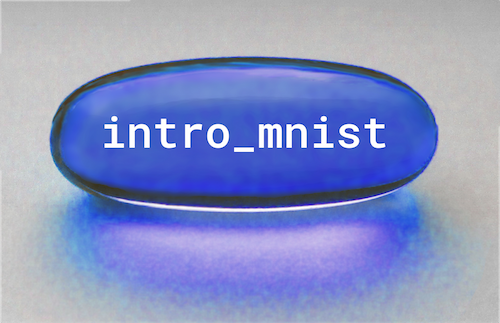
\includegraphics[width=.45\textwidth]{../SOURCE/images/blue_pill.png}

\includegraphics[width=.45\textwidth]{../SOURCE/images/red_pill.png}
\end{center}

Ⓒ 如果你已下定决心准备学习和安装TensorFlow,你可以略过这些文字,直接阅读
后面的章节\footnote{\textbf{推荐随后阅读内容}:\hyperref[download_install]{1 下载与安装}, \hyperref[basic_usage]{2 基本使用}, \hyperref[tf_mech101]{3 TensorFlow 101}.}。不用担心,你仍然会看到MNIST---在阐述TensorFlow的特性时,
我们还会使用MNIST作为一个样例。


%!TEX program = xelatex
% Encoding: UTF8
% SEIKA 2016 | seika@live.ca

% Chapter 1
% Section 1.2 OS_Setup


\section {Download and Setup   ||   下载与安装} \label{download_install}

Ⓔ \textcolor{etc}{You can install TensorFlow either from our provided binary packages or from the github source.}

Ⓒ 您可以使用我们提供的二进制包,或者源代码,安装 TensorFlow.

%
%%
\subsection {Requirements  |  安装需求}

Ⓔ \textcolor{etc}{The TensorFlow Python API currently supports Python 2.7 and Python 3.3+ from source.}

Ⓒ TensorFlow Python API 目前支持 Python 2.7 和 python 3.3以上版本.

Ⓔ \textcolor{etc}{The GPU version (Linux only) currently requires the Cuda Toolkit 7.0 and CUDNN 6.5 V2. Please see \hyperref[install_cuda]{Cuda installation}.}

Ⓒ 支持 GPU 运算的版本 (仅限Linux) 需要 Cuda Toolkit 7.0 和 CUDNN 6.5 V2. 具体请参考\hyperref[install_cuda]{Cuda安装}.

%
%%
\subsection {Overview  |  安装总述}

We support different ways to install TensorFlow:

TensorFlow 支持通过以下不同的方式安装:

\begin{itemize}
\item \hyperref[pip_install]{Pip Install}: \textcolor{etc}{Install TensorFlow on your machine, possibly upgrading previously installed Python packages. May impact existing Python programs on your machine.}\\
\item \hyperref[pip_install]{Pip 安装}: 在你的机器上安装TensorFlow,可能会同时更新之前安装的Python包,并且影响到你机器当前可运行的Python程序.\\
\item \hyperref[virtualenv_install]{Virtualenv Install}: \textcolor{etc}{Install TensorFlow in its own directory, not impacting any existing Python programs on your machine.}\\
\item \hyperref[virtualenv_install]{Virtualenv 安装}: 在一个独立的路径下安装TensorFlow,不会影响到你机器当前运行的Python程序.\\
\item \hyperref[docker_install]{Docker Install}: \textcolor{etc}{Run TensorFlow in a Docker container isolated from all other programs on your machine.}\\
\item \hyperref[docker_install]{Docker 安装}: 在一个独立的Docker容器中安装TensorFlow,并且不会影响到你机器上的任何其他程序.
\end{itemize}

Ⓔ \textcolor{etc}{If you are familiar with Pip, Virtualenv, or Docker, please feel free to adapt the instructions to your particular needs. The names of the pip and Docker images are listed in the corresponding installation sections.}

Ⓒ 如果你已经很熟悉Pip、Virtualenv、Docker这些工具的使用,请利用教程中提供的代码,根据你的需求安装TensorFlow.你会在下文的对应的安装教程中找到Pip或Docker安装所需的镜像.

Ⓔ \textcolor{etc}{If you encounter installation errors, see common problems for some solutions.}

Ⓒ 如果你遇到了安装错误,请参考章节\hyperref[comm_prob]{常见问题}寻找解决方案.

%
%%
\subsection {Pip Installatioin  |  Pip 安装} \label{pip_install}

Ⓔ \textcolor{etc}{\href{https://en.wikipedia.org/wiki/Pip_(package_manager)}{Pip} is a package management system used to install and manage software packages written in Python.}

Ⓒ \href{https://en.wikipedia.org/wiki/Pip_(package_manager)}{Pip} 是一个用于安装和管理Python软件包的管理系统.

Ⓔ \textcolor{etc}{The packages that will be installed or upgraded during the pip install are listed in the \href{https://github.com/tensorflow/tensorflow/blob/master/tensorflow/tools/pip_package/setup.py}{REQUIRED\_PACKAGES section of setup.py}}

Ⓒ 安装依赖包(\href{https://github.com/tensorflow/tensorflow/blob/master/tensorflow/tools/pip_package/setup.py}{REQUIRED\_PACKAGES section of setup.py}) 列出了pip安装时将会被安装或更新的库文件.

Ⓔ \textcolor{etc}{Install pip (or pip3 for python3) if it is not already installed:}

Ⓒ 如果pip尚未被安装,请使用以下代码先安装pip(如果你使用的是Python 3请安装 pip3 ):

\begin{lstlisting}[language = bash]
# Ubuntu/Linux 64-bit
$ sudo apt-get install python-pip python-dev
\end{lstlisting}

\begin{lstlisting}
# Mac OS X
$ sudo easy_install pip
\end{lstlisting}

Ⓔ \textcolor{etc}{Install TensorFlow:}

Ⓒ 安装 TensorFlow:

\begin{lstlisting}
# Ubuntu/Linux 64-bit, CPU only:
$ sudo pip install --upgrade https://storage.googleapis.com/tensorflow/linux/cpu/tensorflow-0.6.0-cp27-none-linux_x86_64.whl
\end{lstlisting}

\begin{lstlisting}
# Ubuntu/Linux 64-bit, GPU enabled:
$ sudo pip install --upgrade https://storage.googleapis.com/tensorflow/linux/gpu/tensorflow-0.6.0-cp27-none-linux_x86_64.whl
\end{lstlisting}

\begin{lstlisting}[language = bash]
# Mac OS X, CPU only:
$ sudo easy_install --upgrade six
$ sudo pip install --upgrade https://storage.googleapis.com/tensorflow/mac/tensorflow-0.6.0-py2-none-any.whl
\end{lstlisting}

Ⓔ \textcolor{etc}{For Python 3:}

Ⓒ 基于 Python 3 的 TensorFlow 安装:

\begin{lstlisting}
# Ubuntu/Linux 64-bit, CPU only:
$ sudo pip3 install --upgrade https://storage.googleapis.com/tensorflow/linux/cpu/tensorflow-0.6.0-cp34-none-linux_x86_64.whl
\end{lstlisting}

\begin{lstlisting}
# Ubuntu/Linux 64-bit, GPU enabled:
$ sudo pip3 install --upgrade https://storage.googleapis.com/tensorflow/linux/gpu/tensorflow-0.6.0-cp34-none-linux_x86_64.whl

\end{lstlisting}

\begin{lstlisting}[language = bash]
# Mac OS X, CPU only:
$ sudo easy_install --upgrade six
$ sudo pip3 install --upgrade https://storage.googleapis.com/tensorflow/mac/tensorflow-0.6.0-py3-none-any.whl
\end{lstlisting}

Ⓔ \textcolor{etc}{You can now test your \hyperref[test_install]{installation}.}

Ⓒ 至此你可以\hyperref[test_install]{测试安装}是否成功.


%
%%
\subsection {Virtualenv installation  |  基于 Virtualenv 安装} \label{virtualenv_install}

Ⓔ \textcolor{etc}{\href{http://docs.python-guide.org/en/latest/dev/virtualenvs/}{Virtualenv} is a tool to keep the dependencies required by different Python projects in separate places. The Virtualenv installation of TensorFlow will not override pre-existing version of the Python packages needed by TensorFlow.}

Ⓒ \href{http://docs.python-guide.org/en/latest/dev/virtualenvs/}{Virtualenv} 是一个管理在不同位置存放和调用 Python 项目所需依赖库的工具. TensorFlow 的 Virtualenv 安装不会覆盖先前已安装的 TensorFlow Python依赖包.

Ⓔ \textcolor{etc}{With \href{https://pypi.python.org/pypi/virtualenv}{Virtualenv} the installation is as follows:}

Ⓒ 基于\href{https://pypi.python.org/pypi/virtualenv}{Virtualenv}的安装分为以下几步:

\begin{itemize}
\item \textcolor{etc}{Install pip and Virtualenv.}
\item \textcolor{etc}{Create a Virtualenv environment.}
\item \textcolor{etc}{Activate the Virtualenv environment and install TensorFlow in it.}
\item \textcolor{etc}{After the install you will activate the Virtualenv environment each time you want to use TensorFlow.}
\item 安装 pip 和 Virtualenv.
\item 建立一个 Virtualenv 环境.
\item 激活这个 Virtualenv 环境,并且在此环境下安装 TensorFlow.
\item 安装完成之后,每次你需要使用TensorFlow之前必须激活这个Virtualenv 环境.
\end{itemize}

Ⓔ \textcolor{etc}{Install pip and Virtualenv:}

Ⓒ 安装 pip 和 Virtualenv:

\begin{lstlisting}
# Ubuntu/Linux 64-bit
$ sudo apt-get install python-pip python-dev python-virtualenv
\end{lstlisting}

\begin{lstlisting}
# Mac OS X
$ sudo easy_install pip
$ sudo pip install --upgrade virtualenv
\end{lstlisting}

Ⓔ \textcolo{etc}{Create a Virtualenv environment in the directory} \lstinline{~/tensorflow}:

Ⓒ 在\lstinline{~/tensorflow}路径下建立一个 Virtualenv 环境:

\begin{lstlisting}
$ virtualenv --system-site-packages ~/tensorflow
\end{lstlisting}

Ⓔ \textcolor{etc}{Activate the environment and use pip to install TensorFlow inside it:}

Ⓒ 激活 Virtualenv 环境并使用pip在该环境下安装TensorFlow:

\begin{lstlisting}
$ source ~/tensorflow/bin/activate  # If using bash
$ source ~/tensorflow/bin/activate.csh  # If using csh
(tensorflow)$  # Your prompt should change

# Ubuntu/Linux 64-bit, CPU only:
(tensorflow)$ pip install --upgrade https://storage.googleapis.com/tensorflow/linux/cpu/tensorflow-0.5.0-cp27-none-linux_x86_64.whl

# Ubuntu/Linux 64-bit, GPU enabled:
(tensorflow)$ pip install --upgrade https://storage.googleapis.com/tensorflow/linux/gpu/tensorflow-0.5.0-cp27-none-linux_x86_64.whl

# Mac OS X, CPU only:
(tensorflow)$ pip install --upgrade https://storage.googleapis.com/tensorflow/mac/tensorflow-0.5.0-py2-none-any.whl
\end{lstlisting}

Ⓔ and again for python3:

\begin{lstlisting}
$ source ~/tensorflow/bin/activate  # If using bash
$ source ~/tensorflow/bin/activate.csh  # If using csh
(tensorflow)$  # Your prompt should change

# Ubuntu/Linux 64-bit, CPU only:
(tensorflow)$ pip install --upgrade https://storage.googleapis.com/tensorflow/linux/cpu/tensorflow-0.6.0-cp34-none-linux_x86_64.whl

# Ubuntu/Linux 64-bit, GPU enabled:
(tensorflow)$ pip install --upgrade https://storage.googleapis.com/tensorflow/linux/gpu/tensorflow-0.6.0-cp34-none-linux_x86_64.whl

# Mac OS X, CPU only:
(tensorflow)$ pip3 install --upgrade https://storage.googleapis.com/tensorflow/mac/tensorflow-0.6.0-py3-none-any.whl
\end{lstlisting}

Ⓔ \textcolor{etc}{With the Virtualenv environment activated, you can now \hyperref[test_install]{test your installation}.}

Ⓒ 在 Virtualenv 环境被激活时,您可以\hyperref[test_install]{测试安装}.

Ⓔ \textcolor{etc}{When you are done using TensorFlow, deactivate the environment.}

Ⓒ 当您无需使用 TensorFlow 时,取消激活该环境.

\begin{lstlisting}
(tensorflow)$ deactivate
$  # Your prompt should change back
\end{lstlisting}

Ⓔ \textcolor{etc}{To use TensorFlow later you will have to activate the Virtualenv environment again:}

Ⓒ 如果需要再次使用 TensorFlow 您需要先再次激活 Virtualenv 环境:

\begin{lstlisting}
$ source ~/tensorflow/bin/activate  # If using bash.
$ source ~/tensorflow/bin/activate.csh  # If using csh.
(tensorflow)$  # Your prompt should change.
# Run Python programs that use TensorFlow.
...
# When you are done using TensorFlow, deactivate the environment.
(tensorflow)$ deactivate
\end{lstlisting}

%%%%%%%%%%%%%%%%
% Done to here %
%%%%%%%%%%%%%%%%

%
%%
\subsection {Docker Installation} \label{docker_install}
\href{http://docker.com/}{Docker} is a system to build self contained versions of a Linux operating system running on your machine. When you install and run TensorFlow via Docker it completely isolates the installation from pre-existing packages on your machine.

We provide 4 Docker images:

\begin{itemize}
\item \lstinline{b.gcr.io/tensorflow/tensorflow}: TensorFlow CPU binary image.
\item \lstinline{b.gcr.io/tensorflow/tensorflow:latest-devel}:CPU Binary image plus source code.
\item \lstinline{b.gcr.io/tensorflow/tensorflow:latest-gpu}:TensorFlow GPU binary image.
\item \lstinline{b.gcr.io/tensorflow/tensorflow:latest-devel-gpu}:GPU Binary image plus source code.
\end{itemize}

We also have tags with latest replaced by a released version (eg \lstinline{0.6.0-gpu}).

With Docker the installation is as follows:

\begin{itemize}
\item Install Docker on your machine.
\item Create a \href{http://docs.docker.com/engine/installation/ubuntulinux/#create-a-docker-group}{Docker group} to allow launching containers without sudo.
\item Launch a Docker container with the TensorFlow image. The image gets downloaded automatically on first launch.
\end{itemize}

See \href{http://docs.docker.com/engine/installation/}{installing Docker} for instructions on installing Docker on your machine.

After Docker is installed, launch a Docker container with the TensorFlow binary image as follows.

\begin{lstlisting}
$ docker run -it b.gcr.io/tensorflow/tensorflow
\end{lstlisting}

If you're using a container with GPU support, some additional flags must be passed to expose the GPU device to the container. For the default config, we include a \href{https://github.com/tensorflow/tensorflow/blob/master/tensorflow/tools/docker/docker_run_gpu.sh}{script} in the repo with these flags, so the command-line would look like:

\begin{lstlisting}
$ path/to/repo/tensorflow/tools/docker/docker_run_gpu.sh b.gcr.io/tensorflow/tensorflow:gpu
\end{lstlisting}

You can now \hyperref[test_install]{test your installation} within the Docker container.


%
%%
%✠% \subsection {Test the TensorFlow Installation} \label{test_install}
\subsection {Test the TensorFlow installation  |  测试 TensorFlow 安装} \label{test_install}

%%%
\subsubsection {(Optional, Linux) Enable GPU Support}

If you installed the GPU version of TensorFlow, you must also install the Cuda Toolkit~7.0 and CUDNN~6.5~V2. Please see \hyperref[install_cuda]{Cuda installation}.

如果您安装了GPU版本的TensorFlow, 您还需要安装 Cuda Toolkit~7.0 和 CUDNN~6.5~V2。请参阅\hyperref[install_cuda]{Cuda 安装}。

You also need to set the \lstinline{LD_LIBRARY_PATH} and \lstinline{CUDA_HOME} environment variables. Consider adding the commands below to your \lstinline{~/.bash_profile}. These assume your CUDA installation is in \lstinline{/usr/local/cuda}:

您需要在先环境变量中设置\lstinline{LD_LIBRARY_PATH} 和 \lstinline{CUDA_HOME}。您可以在\lstinline{~/.bash_profile}中追加一下命令,假设您的CUDA安装位置为\lstinline{/usr/local/cuda}:

\begin{lstlisting}
export LD_LIBRARY_PATH="$LD_LIBRARY_PATH:/usr/local/cuda/lib64"
export CUDA_HOME=/usr/local/cuda
\end{lstlisting}

%%%
\subsubsection {Run TensorFlow from the Command Line  |  从命令行运行TensorFlow}

See \hyperref[comm_prob]{common problems} if an error happens.

如果遇到任何报错,请参考\hyperref[comm_prob]{常见问题}。

Open a terminal and type the following:

打开终端,输入以下指令:

\begin{lstlisting}
$ python
...
>>> import tensorflow as tf
>>> hello = tf.constant('Hello, TensorFlow!')
>>> sess = tf.Session()
>>> print(sess.run(hello))
Hello, TensorFlow!
>>> a = tf.constant(10)
>>> b = tf.constant(32)
>>> print(sess.run(a + b))
42
>>>
\end{lstlisting}

%%%
\subsubsection {Run a TensorFlow demo model  |  运行一个TensorFlow的演示模型}

All TensorFlow packages, including the demo models, are installed in the Python library. The exact location of the Python library depends on your system, but is usually one of:

所有版本的TensorFlow的Python库中包都附带了一些演示模型。 具体位位置取决于您的系统,它们通常会在以下位置出现:

\begin{lstlisting}
/usr/local/lib/python2.7/dist-packages/tensorflow
/usr/local/lib/python2.7/site-packages/tensorflow
\end{lstlisting}

You can find out the directory with the following command:
您可以用以下指令找到它的路径:

\begin{lstlisting}
$ python -c 'import site; print("\n".join(site.getsitepackages()))'
\end{lstlisting}

The simple demo model for classifying handwritten digits from the MNIST dataset is in the sub-directory \lstinline{models/image/mnist/convolutional.py}. You can run it from the command line as follows:

在子目录\lstinline{models/image/mnist/convolutional.py}可以找到一个使用MNIST数据集进行手写数字识别的简单案例。您可以使用以下指令在命令行中直接运行:

\begin{lstlisting}
# Using 'python -m' to find the program in the python search path:
$ python -m tensorflow.models.image.mnist.convolutional
Extracting data/train-images-idx3-ubyte.gz
Extracting data/train-labels-idx1-ubyte.gz
Extracting data/t10k-images-idx3-ubyte.gz
Extracting data/t10k-labels-idx1-ubyte.gz
...etc...

# You can alternatively pass the path to the model program file to the python interpreter.
$ python /usr/local/lib/python2.7/dist-packages/tensorflow/models/image/mnist/convolutional.py
...
\end{lstlisting}


%
%%
\subsection {Installing from source}
When installing from source you will build a pip wheel that you then install using pip. You'll need pip for that, so install it as described \hyperref[pip_install]{above}.

%%%
\subsubsection {Clone the TensorFlow repository}
\begin{lstlisting}
$ git clone --recurse-submodules https://github.com/tensorflow/tensorflow
\end{lstlisting}
\lstinline{--recurse-submodules} is required to fetch the protobuf library that TensorFlow depends on.


%%%
\subsubsection {Installation for Linux}

\paragraph{Install Bazel}

Follow instructions here to install the dependencies for Bazel. Then download bazel version 0.1.1 using the installer for your system and run the installer as mentioned there:

\begin{lstlisting}
$ chmod +x PATH_TO_INSTALL.SH
$ ./PATH_TO_INSTALL.SH --user
\end{lstlisting}

Remember to replace \lstinline{PATH_TO_INSTALL.SH} with the location where you downloaded the installer.

Finally, follow the instructions in that script to place bazel into your binary path.

\paragraph{Install other dependencies}\\

\begin{lstlisting}
$ sudo apt-get install python-numpy swig python-dev
\end{lstlisting}

\paragraph{Configure the installation}

Run the configure script at the root of the tree. The configure script asks you for the path to your python interpreter and allows (optional) configuration of the CUDA libraries (see \hyperref[install_cuda]{below}).

This step is used to locate the python and numpy header files.

\begin{lstlisting}
$ ./configure
Please specify the location of python. [Default is /usr/bin/python]:
\end{lstlisting}

\paragraph{Optional: Install CUDA (GPUs on Linux)} \label{install_cuda}

In order to build or run TensorFlow with GPU support, both Cuda Toolkit 7.0 and CUDNN 6.5 V2 from NVIDIA need to be installed.

TensorFlow GPU support requires having a GPU card with NVidia Compute Capability >= 3.5. Supported cards include but are not limited to:

\begin{itemize}
\item NVidia Titan
\item NVidia Titan X
\item NVidia K20
\item NVidia K40
\end{itemize}

Download and install Cuda Toolkit 7.0

https://developer.nvidia.com/cuda-toolkit-70

Install the toolkit into e.g. /usr/local/cuda

Download and install CUDNN Toolkit 6.5

https://developer.nvidia.com/rdp/cudnn-archive

Uncompress and copy the cudnn files into the toolkit directory. Assuming the toolkit is installed in /usr/local/cuda:

\begin{lstlisting}
tar xvzf cudnn-6.5-linux-x64-v2.tgz
sudo cp cudnn-6.5-linux-x64-v2/cudnn.h /usr/local/cuda/include
sudo cp cudnn-6.5-linux-x64-v2/libcudnn* /usr/local/cuda/lib64
\end{lstlisting}

Configure TensorFlow's canonical view of Cuda libraries

When running the configure script from the root of your source tree, select the option Y when asked to build TensorFlow with GPU support.

\begin{lstlisting}
$ ./configure
Please specify the location of python. [Default is /usr/bin/python]:
Do you wish to build TensorFlow with GPU support? [y/N] y
GPU support will be enabled for TensorFlow

Please specify the location where CUDA 7.0 toolkit is installed. Refer to
README.md for more details. [default is: /usr/local/cuda]: /usr/local/cuda

Please specify the location where CUDNN 6.5 V2 library is installed. Refer to
README.md for more details. [default is: /usr/local/cuda]: /usr/local/cuda

Setting up Cuda include
Setting up Cuda lib64
Setting up Cuda bin
Setting up Cuda nvvm
Configuration finished
\end{lstlisting}

This creates a canonical set of symbolic links to the Cuda libraries on your system. Every time you change the Cuda library paths you need to run this step again before you invoke the bazel build command.

Build your target with GPU support

From the root of your source tree, run:

\begin{lstlisting}
$ bazel build -c opt --config=cuda //tensorflow/cc:tutorials_example_trainer

$ bazel-bin/tensorflow/cc/tutorials_example_trainer --use_gpu
# Lots of output. This tutorial iteratively calculates the major eigenvalue of
# a 2x2 matrix, on GPU. The last few lines look like this.
000009/000005 lambda = 2.000000 x = [0.894427 -0.447214] y = [1.788854 -0.894427]
000006/000001 lambda = 2.000000 x = [0.894427 -0.447214] y = [1.788854 -0.894427]
000009/000009 lambda = 2.000000 x = [0.894427 -0.447214] y = [1.788854 -0.894427]
\end{lstlisting}

Note that "--config=cuda" is needed to enable the GPU support.

Enabling Cuda 3.0

TensorFlow officially supports Cuda devices with 3.5 and 5.2 compute capabilities. In order to enable earlier Cuda devices such as Grid K520, you need to target Cuda 3.0. This can be done through TensorFlow unofficial settings with "configure".

\begin{lstlisting}
$ TF_UNOFFICIAL_SETTING=1 ./configure

# Same as the official settings above

WARNING: You are configuring unofficial settings in TensorFlow. Because some
external libraries are not backward compatible, these settings are largely
untested and unsupported.

Please specify a list of comma-separated Cuda compute capabilities you want to
build with. You can find the compute capability of your device at:
https://developer.nvidia.com/cuda-gpus.
Please note that each additional compute capability significantly increases
your build time and binary size. [Default is: "3.5,5.2"]: 3.0

Setting up Cuda include
Setting up Cuda lib64
Setting up Cuda bin
Setting up Cuda nvvm
Configuration finished
\end{lstlisting}

Known issues

Although it is possible to build both Cuda and non-Cuda configs under the same source tree, we recommend to run \"bazel clean\" when switching between these two configs in the same source tree.

You have to run configure before running bazel build. Otherwise, the build will fail with a clear error message. In the future, we might consider making this more conveninent by including the configure step in our build process, given necessary bazel new feature support.


%%%
\subsubsection {Installation for Mac OS X}

We recommend using \href{http://brew.sh/}{homebrew} to install the bazel and SWIG dependencies, and installing python dependencies using easy_install or pip.

\paragraph{Dependencies}

Follow instructions here to install the dependencies for Bazel. You can then use homebrew to install bazel and SWIG:

\begin{lstlisting}
$ brew install bazel swig
\end{lstlisting}

You can install the python dependencies using easy_install or pip. Using easy_install, run

\begin{lstlisting}
$ sudo easy_install -U six
$ sudo easy_install -U numpy
$ sudo easy_install wheel
\end{lstlisting}

We also recommend the \href{https://ipython.org/}{ipython} enhanced python shell, so best install that too:

\begin{lstlisting}
$ sudo easy_install ipython
\end{lstlisting}

\paragraph{Configure the installation}

Run the \lstinline{configure} script at the root of the tree. The configure script asks you for the path to your python interpreter.

This step is used to locate the python and numpy header files.

\begin{lstlisting}
$ ./configure
Please specify the location of python. [Default is /usr/bin/python]:
Do you wish to build TensorFlow with GPU support? [y/N]
\end{lstlisting}

%%%
\subsubsection {Create the pip package and install}

\begin{lstlisting}
$ bazel build -c opt //tensorflow/tools/pip_package:build_pip_package

# To build with GPU support:
$ bazel build -c opt --config=cuda //tensorflow/tools/pip_package:build_pip_package

$ bazel-bin/tensorflow/tools/pip_package/build_pip_package /tmp/tensorflow_pkg

# The name of the .whl file will depend on your platform.
$ pip install /tmp/tensorflow_pkg/tensorflow-0.5.0-cp27-none-linux_x86_64.whl
\end{lstlisting}

%
%%
\subsection {Train your first TensorFlow neural net model  |  训练第一个TensorFlow模型}

Starting from the root of your source tree, run:

从根目录开始运行一下指令:

\begin{lstlisting}
$ cd tensorflow/models/image/mnist
$ python convolutional.py
Succesfully downloaded train-images-idx3-ubyte.gz 9912422 bytes.
Succesfully downloaded train-labels-idx1-ubyte.gz 28881 bytes.
Succesfully downloaded t10k-images-idx3-ubyte.gz 1648877 bytes.
Succesfully downloaded t10k-labels-idx1-ubyte.gz 4542 bytes.
Extracting data/train-images-idx3-ubyte.gz
Extracting data/train-labels-idx1-ubyte.gz
Extracting data/t10k-images-idx3-ubyte.gz
Extracting data/t10k-labels-idx1-ubyte.gz
Initialized!
Epoch 0.00
Minibatch loss: 12.054, learning rate: 0.010000
Minibatch error: 90.6%
Validation error: 84.6%
Epoch 0.12
Minibatch loss: 3.285, learning rate: 0.010000
Minibatch error: 6.2%
Validation error: 7.0%
...
...
\end{lstlisting}


%
%%

% \subsection {Common Problems} \label{comm_prob}
\subsection {Common Problems  |  常见问题} \label{comm_prob}

%%%
\subsubsection {GPU-related issues  |  GPU有关问题}

If you encounter the following when trying to run a TensorFlow program:

\begin{lstlisting}
ImportError: libcudart.so.7.0: cannot open shared object file: No such file or directory
\end{lstlisting}

Make sure you followed the the GPU installation \hyperref[install_cuda]{instructions}.

%%%
\subsubsection {Pip installation issues  |  Pip安装中的问题}

\paragraph{\lstinline{Can't find setup.py}}

If, during pip install, you encounter an error like:

\begin{lstlisting}
...
IOError: [Errno 2] No such file or directory: '/tmp/pip-o6Tpui-build/setup.py'
\end{lstlisting}

Solution: upgrade your version of pip:

\begin{lstlisting}
pip install --upgrade pip
\end{lstlisting}

This may require sudo, depending on how pip is installed.

\paragraph{\lstinline{SSLError: SSL_VERIFY_FAILED}}

If, during pip install from a URL, you encounter an error like:

\begin{lstlisting}
...
SSLError: [SSL: CERTIFICATE_VERIFY_FAILED] certificate verify failed
\end{lstlisting}

Solution: Download the wheel manually via curl or wget, and pip install locally.

%%%
\subsubsection {Linux issues}

If you encounter:

\begin{lstlisting}
...
 "__add__", "__radd__",
             ^
SyntaxError: invalid syntax
\end{lstlisting}

Solution: make sure you are using Python 2.7.

%%%
\subsubsection {Mac OS X: ImportError: No module named copyreg}

On Mac OS X, you may encounter the following when importing tensorflow.

\begin{lstlisting}
>>> import tensorflow as tf
...
ImportError: No module named copyreg
\end{lstlisting}

Solution: TensorFlow depends on protobuf, which requires the Python package \lstinline{six-1.10.0}. Apple's default Python installation only provides \lstinline{six-1.4.1}.

You can resolve the issue in one of the following ways:
\begin{itemize}
\item pgrade the Python installation with the current version of \lstinline{six}:
\begin{lstlisting}
$ sudo easy_install -U six
\end{lstlisting}

\item Install TensorFlow with a separate Python library:
  \begin{itemize}
  \item Virtualenv
  \item Docker
  \end{itemize}
Install a separate copy of Python via Homebrew or MacPorts and re-install TensorFlow in that copy of Python.
\end{itemize}




%%%
\subsubsection {Mac OS X: TypeError: \lstinline{__init__()} got an unexpected keyword argument 'syntax'}

On Mac OS X, you may encounter the following when importing tensorflow.

\begin{lstlisting}
>>> import tensorflow as tf
Traceback (most recent call last):
  File "<stdin>", line 1, in <module>
  File "/usr/local/lib/python2.7/site-packages/tensorflow/__init__.py", line 4, in <module>
    from tensorflow.python import *
  File "/usr/local/lib/python2.7/site-packages/tensorflow/python/__init__.py", line 13, in <module>
    from tensorflow.core.framework.graph_pb2 import *
...
  File "/usr/local/lib/python2.7/site-packages/tensorflow/core/framework/tensor_shape_pb2.py", line 22, in <module>
    serialized_pb=_b('\n,tensorflow/core/framework/tensor_shape.proto\x12\ntensorflow\"d\n\x10TensorShapeProto\x12-\n\x03\x64im\x18\x02 \x03(\x0b\x32 .tensorflow.TensorShapeProto.Dim\x1a!\n\x03\x44im\x12\x0c\n\x04size\x18\x01 \x01(\x03\x12\x0c\n\x04name\x18\x02 \x01(\tb\x06proto3')
TypeError: __init__() got an unexpected keyword argument 'syntax'
\end{lstlisting}

This is due to a conflict between protobuf versions (we require protobuf 3.0.0). The best current solution is to make sure older versions of protobuf are not installed, such as:

\begin{lstlisting}
$ pip install --upgrade protobuf
\end{lstlisting}



%%%% ## 二进制安装 <a class="md-anchor" id="AUTOGENERATED-binary-installation"></a>

%%%% TensorFlow Python API 依赖 Python 2.7 版本.

%%%% 在 Linux 和 Mac 下最简单的安装方式, 是使用 [pip](https://pypi.python.org/pypi/pip)
%%%% 安装.

%%%% 如果在安装过程中遇到错误, 请查阅 [常见问题](#common_install_problems).
%%%% 为了简化安装步骤, 建议使用 virtualenv, 教程见 [这里](#virtualenv_install).

%%%% ### Ubuntu/Linux <a class="md-anchor" id="AUTOGENERATED-ubuntu-linux"></a>

%%%% ```bash
%%%% # 仅使用 CPU 的版本
%%%% $ pip install https://storage.googleapis.com/tensorflow/linux/cpu/tensorflow-0.5.0-cp27-none-linux_x86_64.whl

%%%% # 开启 GPU 支持的版本 (安装该版本的前提是已经安装了 CUDA sdk)
%%%% $ pip install https://storage.googleapis.com/tensorflow/linux/gpu/tensorflow-0.5.0-cp27-none-linux_x86_64.whl
%%%% ```

%%%% ### Mac OS X <a class="md-anchor" id="AUTOGENERATED-mac-os-x"></a>

%%%% 在 OS X 系统上, 我们推荐先安装 [homebrew](http://brew.sh), 然后执行
%%%% `brew install python`, 以便能够使用 homebrew 中的 Python 安装
%%%% TensorFlow. 另外一种推荐的方式是在 [virtualenv](#virtualenv_install)
%%%% 中安装 TensorFlow.

%%%% ```bash
%%%% # 当前版本只支持 CPU
%%%% $ pip install https://storage.googleapis.com/tensorflow/mac/tensorflow-0.5.0-py2-none-any.whl
%%%% ```

%%%% ## 基于 Docker 的安装 <a class="md-anchor" id="AUTOGENERATED-docker-based-installation"></a>

%%%% 我们也支持通过 [Docker](http://docker.com/) 运行 TensorFlow.
%%%% 该方式的优点是不用操心软件依赖问题.

%%%% 首先, [安装 Docker](http://docs.docker.com/engine/installation/). 一旦 Docker
%%%% 已经启动运行, 可以通过命令启动一个容器:

%%%% ```bash
%%%% $ docker run -it b.gcr.io/tensorflow/tensorflow
%%%% ```

%%%% 该命令将启动一个已经安装好 TensorFlow 及相关依赖的容器.

%%%% ### 其它镜像 <a class="md-anchor" id="AUTOGENERATED-additional-images"></a>

%%%% 默认的 Docker 镜像只包含启动和运行 TensorFlow 所需依赖库的一个最小集. 我们额外提供了
%%%% 下面的容器, 该容器同样可以通过上述 `docker run` 命令安装:

%%%% * `b.gcr.io/tensorflow/tensorflow-full`: 镜像中的 TensorFlow 是从源代码完整安装的,
  %%%% 包含了编译和运行 TensorFlow 所需的全部工具. 在该镜像上, 可以直接使用源代码进行实验,
  %%%% 而不需要再安装上述的任何依赖.
 %%%%
%%%% ## 基于 VirtualEnv 的安装 <a class="md-anchor" id="virtualenv_install"></a>

%%%% 我们推荐使用 [virtualenv](https://pypi.python.org/pypi/virtualenv) 创建一个隔离的容器, 来安装 TensorFlow. 这是可选的, 但是这样做能使排查安装问题变得更容易.

%%%% 首先, 安装所有必备工具:

%%%% ```bash
%%%% # 在 Linux 上:
%%%% $ sudo apt-get install python-pip python-dev python-virtualenv

%%%% # 在 Mac 上:
%%%% $ sudo easy_install pip  # 如果还没有安装 pip
%%%% $ sudo pip install --upgrade virtualenv
%%%% ```

%%%% 接下来, 建立一个全新的 virtualenv 环境. 为了将环境建在 `~/tensorflow`
%%%% 目录下, 执行:

%%%% ```bash
%%%% $ virtualenv --system-site-packages ~/tensorflow
%%%% $ cd ~/tensorflow
%%%% ```

%%%% 然后, 激活 virtualenv:

%%%% ```bash
%%%% $ source bin/activate  # 如果使用 bash
%%%% $ source bin/activate.csh  # 如果使用 csh
%%%% (tensorflow)$  # 终端提示符应该发生变化
%%%% ```

%%%% 在 virtualenv 内, 安装 TensorFlow:

%%%% ```bash
%%%% (tensorflow)$ pip install --upgrade <$url_to_binary.whl>
%%%% ```

%%%% 接下来, 使用类似命令运行 TensorFlow 程序:

%%%% ```bash
%%%% (tensorflow)$ cd tensorflow/models/image/mnist
%%%% (tensorflow)$ python convolutional.py

%%%% # 当使用完 TensorFlow
%%%% (tensorflow)$ deactivate  # 停用 virtualenv

%%%% $  # 你的命令提示符会恢复原样
%%%% ```

%%%% ## 尝试你的第一个 TensorFlow 程序 <a class="md-anchor" id="AUTOGENERATED-try-your-first-tensorflow-program"></a>

%%%% ### (可选) 启用 GPU 支持 <a class="md-anchor" id="AUTOGENERATED--optional--enable-gpu-support"></a>

%%%% 如果你使用 pip 二进制包安装了开启 GPU 支持的 TensorFlow, 你必须确保
%%%% 系统里安装了正确的 CUDA sdk 和 CUDNN 版本. 请参间  [CUDA 安装教程](#install_cuda)

%%%% 你还需要设置 `LD_LIBRARY_PATH` 和 `CUDA_HOME` 环境变量. 可以考虑将下面的命令
%%%% 添加到 `~/.bash_profile` 文件中, 这样每次登陆后自动生效. 注意, 下面的命令
%%%% 假定 CUDA 安装目录为 `/usr/local/cuda`:

%%%% ```bash
%%%% export LD_LIBRARY_PATH="$LD_LIBRARY_PATH:/usr/local/cuda/lib64"
%%%% export CUDA_HOME=/usr/local/cuda
%%%% ```

%%%% ### 运行 TensorFlow <a class="md-anchor" id="AUTOGENERATED-run-tensorflow"></a>

%%%% 打开一个 python 终端:

%%%% ```bash
%%%% $ python

%%%% >>> import tensorflow as tf
%%%% >>> hello = tf.constant('Hello, TensorFlow!')
%%%% >>> sess = tf.Session()
%%%% >>> print sess.run(hello)
%%%% Hello, TensorFlow!
%%%% >>> a = tf.constant(10)
%%%% >>> b = tf.constant(32)
%%%% >>> print sess.run(a+b)
%%%% 42
%%%% >>>

%%%% ```

%%%% ## 从源码安装 <a class="md-anchor" id="source"></a>

%%%% ### 克隆 TensorFlow 仓库 <a class="md-anchor" id="AUTOGENERATED-clone-the-tensorflow-repository"></a>

%%%% ```bash
%%%% $ git clone --recurse-submodules https://github.com/tensorflow/tensorflow
%%%% ```

%%%% `--recurse-submodules` 参数是必须得, 用于获取 TesorFlow 依赖的 protobuf 库.

%%%% ### Linux 安装 <a class="md-anchor" id="AUTOGENERATED-installation-for-linux"></a>

%%%% #### 安装 Bazel <a class="md-anchor" id="AUTOGENERATED-install-bazel"></a>

%%%% 首先依照 [教程](http://bazel.io/docs/install.html) 安装 Bazel 的依赖.
%%%% 然后使用下列命令下载和编译 Bazel 的源码:

%%%% ```bash
%%%% $ git clone https://github.com/bazelbuild/bazel.git
%%%% $ cd bazel
%%%% $ git checkout tags/0.1.0
%%%% $ ./compile.sh
%%%% ```

%%%% 上面命令中拉取的代码标签为 `0.1.0`, 兼容 Tensorflow 目前版本. bazel 的`HEAD` 版本 (即最新版本) 在这里可能不稳定.

%%%% 将执行路径 `output/bazel` 添加到 `$PATH` 环境变量中.

%%%% #### 安装其他依赖 <a class="md-anchor" id="AUTOGENERATED-install-other-dependencies"></a>

%%%% ```bash
%%%% $ sudo apt-get install python-numpy swig python-dev
%%%% ```

%%%% #### 可选: 安装 CUDA (在 Linux 上开启 GPU 支持) <a class="md-anchor" id="install_cuda"></a>

%%%% 为了编译并运行能够使用 GPU 的 TensorFlow, 需要先安装 NVIDIA 提供的 Cuda Toolkit 7.0
%%%% 和 CUDNN 6.5 V2.

%%%% TensorFlow 的 GPU 特性只支持 NVidia Compute Capability >= 3.5 的显卡. 被支持的显卡
%%%% 包括但不限于:

%%%% * NVidia Titan
%%%% * NVidia Titan X
%%%% * NVidia K20
%%%% * NVidia K40

%%%% ##### 下载并安装 Cuda Toolkit 7.0 <a class="md-anchor" id="AUTOGENERATED-download-and-install-cuda-toolkit-7.0"></a>

%%%% [下载地址](https://developer.nvidia.com/cuda-toolkit-70)

%%%% 将工具安装到诸如 `/usr/local/cuda` 之类的路径.

%%%% ##### 下载并安装 CUDNN Toolkit 6.5 <a class="md-anchor" id="AUTOGENERATED-download-and-install-cudnn-toolkit-6.5"></a>

%%%% [下载地址](https://developer.nvidia.com/rdp/cudnn-archive)

%%%% 解压并拷贝 CUDNN 文件到 Cuda Toolkit 7.0 安装路径下. 假设 Cuda Toolkit 7.0 安装
%%%% 在 `/usr/local/cuda`, 执行以下命令:

%%%% ``` bash
%%%% tar xvzf cudnn-6.5-linux-x64-v2.tgz
%%%% sudo cp cudnn-6.5-linux-x64-v2/cudnn.h /usr/local/cuda/include
%%%% sudo cp cudnn-6.5-linux-x64-v2/libcudnn* /usr/local/cuda/lib64
%%%% ```

%%%% ##### 配置 TensorFlow 的 Cuba 选项 <a class="md-anchor" id="AUTOGENERATED-configure-tensorflow-s-canonical-view-of-cuda-libraries"></a>

%%%% 从源码树的根路径执行:

%%%% ``` bash
%%%% $ ./configure
%%%% Do you wish to bulid TensorFlow with GPU support? [y/n] y
%%%% GPU support will be enabled for TensorFlow

%%%% Please specify the location where CUDA 7.0 toolkit is installed. Refer to
%%%% README.md for more details. [default is: /usr/local/cuda]: /usr/local/cuda

%%%% Please specify the location where CUDNN 6.5 V2 library is installed. Refer to
%%%% README.md for more details. [default is: /usr/local/cuda]: /usr/local/cuda

%%%% Setting up Cuda include
%%%% Setting up Cuda lib64
%%%% Setting up Cuda bin
%%%% Setting up Cuda nvvm
%%%% Configuration finished
%%%% ```

%%%% 这些配置将建立到系统 Cuda 库的符号链接. 每当 Cuda 库的路径发生变更时, 必须重新执行上述
%%%% 步骤, 否则无法调用 bazel 编译命令.

%%%% ##### 编译目标程序, 开启 GPU 支持 <a class="md-anchor" id="AUTOGENERATED-build-your-target-with-gpu-support."></a>

%%%% 从源码树的根路径执行:

%%%% ```bash
%%%% $ bazel build -c opt --config=cuda //tensorflow/cc:tutorials_example_trainer

%%%% $ bazel-bin/tensorflow/cc/tutorials_example_trainer --use_gpu
%%%% # 大量的输出信息. 这个例子用 GPU 迭代计算一个 2x2 矩阵的主特征值 (major eigenvalue).
%%%% # 最后几行输出和下面的信息类似.
%%%% 000009/000005 lambda = 2.000000 x = [0.894427 -0.447214] y = [1.788854 -0.894427]
%%%% 000006/000001 lambda = 2.000000 x = [0.894427 -0.447214] y = [1.788854 -0.894427]
%%%% 000009/000009 lambda = 2.000000 x = [0.894427 -0.447214] y = [1.788854 -0.894427]
%%%% ```

%%%% 注意, GPU 支持需通过编译选项 "--config=cuda" 开启.

%%%% ##### 已知问题 <a class="md-anchor" id="AUTOGENERATED-known-issues"></a>

%%%% * 尽管可以在同一个源码树下编译开启 Cuda 支持和禁用 Cuda 支持的版本, 我们还是推荐在
%%%% 在切换这两种不同的编译配置时, 使用 "bazel clean" 清理环境.

%%%% * 在执行 bazel 编译前必须先运行 configure, 否则编译会失败并提示错误信息. 未来,
%%%% 我们可能考虑将 configure 步骤包含在编译过程中, 以简化整个过程, 前提是 bazel 能够提供新的特性支持这样.

%%%% ### Mac OS X 安装 <a class="md-anchor" id="AUTOGENERATED-installation-for-mac-os-x"></a>

%%%% Mac 和 Linux 需要的软件依赖完全一样, 但是安装过程区别很大. 以下链接用于帮助你
%%%% 在 Mac OS X 上安装这些依赖:

%%%% #### Bazel <a class="md-anchor" id="AUTOGENERATED-bazel"></a>

%%%% 参见[本网页](http://bazel.io/docs/install.html)的 Mac OS X 安装指南.

%%%% #### SWIG <a class="md-anchor" id="AUTOGENERATED-swig"></a>

%%%% [Mac OS X 安装教程](http://www.swig.org/Doc3.0/Preface.html#Preface_osx_installation).

%%%% 注意: 你需要安装[PCRE](ftp://ftp.csx.cam.ac.uk/pub/software/programming/pcre/),
%%%% 而*不是* PCRE2.

%%%% #### Numpy <a class="md-anchor" id="AUTOGENERATED-numpy"></a>

%%%% 参见[安装教程](http://docs.scipy.org/doc/numpy/user/install.html).

%%%% ### 创建 pip 包并安装 <a class="md-anchor" id="create-pip"></a>

%%%% ```bash
%%%% $ bazel build -c opt //tensorflow/tools/pip_package:build_pip_package

%%%% $ bazel-bin/tensorflow/tools/pip_package/build_pip_package /tmp/tensorflow_pkg

%%%% # .whl 文件的实际名字与你所使用的平台有关
%%%% $ pip install /tmp/tensorflow_pkg/tensorflow-0.5.0-cp27-none-linux_x86_64.whl
%%%% ```

%%%% ## 训练你的第一个 TensorFlow 神经网络模型 <a class="md-anchor" id="AUTOGENERATED-train-your-first-tensorflow-neural-net-model"></a>

%%%% 从源代码树的根路径执行:

%%%% ```python
%%%% $ cd tensorflow/models/image/mnist
%%%% $ python convolutional.py
%%%% Succesfully downloaded train-images-idx3-ubyte.gz 9912422 bytes.
%%%% Succesfully downloaded train-labels-idx1-ubyte.gz 28881 bytes.
%%%% Succesfully downloaded t10k-images-idx3-ubyte.gz 1648877 bytes.
%%%% Succesfully downloaded t10k-labels-idx1-ubyte.gz 4542 bytes.
%%%% Extracting data/train-images-idx3-ubyte.gz
%%%% Extracting data/train-labels-idx1-ubyte.gz
%%%% Extracting data/t10k-images-idx3-ubyte.gz
%%%% Extracting data/t10k-labels-idx1-ubyte.gz
%%%% Initialized!
%%%% Epoch 0.00
%%%% Minibatch loss: 12.054, learning rate: 0.010000
%%%% Minibatch error: 90.6%
%%%% Validation error: 84.6%
%%%% Epoch 0.12
%%%% Minibatch loss: 3.285, learning rate: 0.010000
%%%% Minibatch error: 6.2%
%%%% Validation error: 7.0%
%%%% ...
%%%% ...
%%%% ```

%%%% ## 常见问题 <a class="md-anchor" id="common_install_problems"></a>

%%%% ### GPU 相关问题 <a class="md-anchor" id="AUTOGENERATED-gpu-related-issues"></a>

%%%% 如果在尝试运行一个 TensorFlow 程序时出现以下错误:

%%%% ```python
%%%% ImportError: libcudart.so.7.0: cannot open shared object file: No such file or directory
%%%% ```

%%%% 请确认你正确安装了 GPU 支持, 参见 [相关章节](#install_cuda).

%%%% ### 在 Linux 上 <a class="md-anchor" id="AUTOGENERATED-on-linux"></a>

%%%% 如果出现错误:

%%%% ```python
%%%% ...
 %%%% "__add__", "__radd__",
             %%%% ^
%%%% SyntaxError: invalid syntax
%%%% ```

%%%% 解决方案: 确认正在使用的 Python 版本为 Python 2.7.

%%%% ### 在 Mac OS X 上 <a class="md-anchor" id="AUTOGENERATED-on-macosx"></a>

%%%% 如果出现错误:

%%%% ```python
%%%% import six.moves.copyreg as copyreg

%%%% ImportError: No module named copyreg
%%%% ```

%%%% 解决方案: TensorFlow 使用的 protobuf 依赖 `six-1.10.0`. 但是, Apple 的默认 python 环境
%%%% 已经安装了 `six-1.4.1`, 该版本可能很难升级. 这里提供几种方法来解决该问题:

%%%% 1. 升级全系统的 `six`:

    %%%% ```bash
    %%%% sudo easy_install -U six
    %%%% ```

%%%% 2. 通过 homebrew 安装一个隔离的 python 副本:

    %%%% ```bash
    %%%% brew install python
    %%%% ```

%%%% 3. 在[`virtualenv`](#virtualenv_install) 内编译或使用 TensorFlow.
%%%%

%%%% 如果出现错误:

%%%% ```
%%%% >>> import tensorflow as tf
%%%% Traceback (most recent call last):
  %%%% File "<stdin>", line 1, in <module>
  %%%% File "/usr/local/lib/python2.7/site-packages/tensorflow/__init__.py", line 4, in <module>
    %%%% from tensorflow.python import *
  %%%% File "/usr/local/lib/python2.7/site-packages/tensorflow/python/__init__.py", line 13, in <module>
    %%%% from tensorflow.core.framework.graph_pb2 import *
%%%% ...
  %%%% File "/usr/local/lib/python2.7/site-packages/tensorflow/core/framework/tensor_shape_pb2.py", line 22, in <module>
    %%%% serialized_pb=_b('\n,tensorflow/core/framework/tensor_shape.proto\x12\ntensorflow\"d\n\x10TensorShapeProto\x12-\n\x03\x64im\x18\x02 \x03(\x0b\x32 .tensorflow.TensorShapeProto.Dim\x1a!\n\x03\x44im\x12\x0c\n\x04size\x18\x01 \x01(\x03\x12\x0c\n\x04name\x18\x02 \x01(\tb\x06proto3')
%%%% TypeError: __init__() got an unexpected keyword argument 'syntax'
%%%% ```

%%%% 这是由于安装了冲突的 protobuf 版本引起的, TensorFlow 需要的是 protobuf 3.0.0. 当前
%%%% 最好的解决方案是确保没有安装旧版本的 protobuf, 可以使用以下命令重新安装 protobuf 来解决
%%%% 冲突:

%%%% ```bash
%%%% brew reinstall --devel protobuf
%%%% ```

%%%% > 原文:[Download and Setup](http://tensorflow.org/get_started/os_setup.md)  翻译:[@doc001](https://github.com/PFZheng)  校对:[@yangtze](https://github.com/sstruct)

%!TEX program = xelatex
% Encoding: UTF8
% SEIKA 2016 | seika@live.ca

% Chapter 1
% Section 1.3 Introduction

\section{Basic Usage   ||   使用基础} \label{basic_usage}

Ⓔ \textcolor{etc}{To use TensorFlow you need to understand how TensorFlow:}

\begin{itemize}
\item \textcolor{etc}{Represents computations as \emph{graphs}.}
\item \textcolor{etc}{Executes graphs in the context of \lstinline{Sessions}.}
\item \textcolor{etc}{Represents data as \emph{tensors}.}
\item \textcolor{etc}{Maintains state with \lstinline{Variables}.}
\item \textcolor{etc}{Uses feeds and fetches to get data into and out of arbitrary operations.}
\end{itemize}

Ⓒ 使用TensorFlow之前你需要了解关于TensorFlow的以下基础知识:

\begin{itemize}
\item 使用\emph{图}(\emph{graphs})来表示计算.\index{graph}
\item 在\emph{会话}(\lstinline{Session})中执行图.\index{session}
\item 使用\emph{张量}(\emph{tensors})来代表数据.\index{tensor}
\item 通过\emph{变量}(\lstinline{Variables})维护状态.\index{variable}
\item 使用\emph{供给}(\lstinline{feeds})和\emph{取回}(\lstinline{fetches})将数据传入或传出任何操作.
\end{itemize}

%
%%
\subsection{Overview  |  总览}

Ⓔ \textcolor{etc}{TensorFlow is a programming system in which you represent computations as graphs. Nodes in the graph are called ops (short for operations). An op takes zero or more \emph{Tensors}, performs some computation, and produces zero or more \emph{Tensors}. A Tensor is a typed multi-dimensional array. For example, you can represent a mini-batch of images as a 4-D array of floating point numbers with dimensions \lstinline{[batch, height, width, channels]}.}

Ⓒ TensorFlow 是一个以\emph{图}(\emph{graphs})来表示计算的编程系统,图中的节点被称之为 op~(operation的缩写). 一个 op 获得零或多个\emph{张量}(\emph{tensors})执行计算,产生零或多个\emph{张量}。\emph{张量} 是一个按类型划分的多维数组。例如, 你可以将一小组图像集表示为一个四维浮点数数组,这四个维度分别是\lstinline{[batch, height, width, channels]}。

Ⓔ \textcolor{etc}{A TensorFlow graph is a description of computations. To compute anything, a graph must be launched in a \lstinline{Session}. A Session places the graph ops onto \lstinline{Devices}, such as CPUs or GPUs, and provides methods to execute them. These methods return tensors produced by ops as \href{http://www.numpy.org/}{numpy} ndarray objects in Python, and as \lstinline{tensorflow::Tensor} instances in C and C++.}

Ⓒ TensorFlow的图是一种对计算的抽象描述。在计算开始前, 图必须在 \emph{会话}(\lstinline{Session()}) 中被启动.\emph{会话}将图的op分发到如 CPU 或 GPU 之类的 \emph{设备}(\lstinline{Devices()}) 上, 同时提供执行 op 的方法。这些方法执行后, 将产生的\emph{张量}(\emph{tensor})返回。在 Python 语言中, 将返回\href{http://www.numpy.org}{numpy}的\lstinline{ndarray} 对象; 在 C 和 C++ 语言中, 将返回\lstinline{tensorflow::Tensor}实例。


%
%%
%✠ \subsection{The computation graph}
\subsection {The computation graph  |  计算图} \label{computation_graph}

Ⓔ \textcolor{etc}{TensorFlow programs are usually structured into a \emph{construction phase}, that assembles a graph, and an \emph{execution phase} that uses a session to execute ops in the graph.}

Ⓒ 通常,TensorFlow编程可按两个阶段组织起来:\emph{构建阶段}和\emph{执行阶段};前者用于组织\emph{计算图},而后者利用session中执行\emph{计算图}中的op操作。

Ⓔ \textcolor{etc}{For example, it is common to create a graph to represent and train a neural network in the construction phase, and then repeatedly execute a set of training ops in the graph in the execution phase.}

Ⓒ 例如,在构建阶段创建一个图来表示和训练神经网络,然后在执行阶段反复执行一组op来实现图中的训练。

Ⓔ \textcolor{etc}{TensorFlow can be used from C, C++, and Python programs. It is presently much easier to use the Python library to assemble graphs, as it provides a large set of helper functions not available in the C and C++ libraries.}

Ⓒ TensorFlow 支持 C、 C++、 Python 编程语言。 目前, TensorFlow 的 Python 库更加易用,它提供了大量的辅助函数来简化构建图的工作, 而这些函数在 C 和 C++ 库中尚不被支持。

Ⓔ \textcolor{etc}{The session libraries have equivalent functionalities for the three languages.}

Ⓒ 这三种语言的会话库 (session libraries) 是一致的.

%%%
% \subsubsection {Building the graph}
\subsubsection {Building the graph  |  构建计算图}

Ⓔ \textcolor{etc}{To build a graph start with ops that do not need any input (source ops), such as Constant, and pass their output to other ops that do computation.}

Ⓒ 刚开始基于op建立图的时候一般不需要任何的输入源(source op),例如输入常量(\lstinline{Constance}),再将它们传递给其它 op 执行运算。

Ⓔ \textcolor{etc}{The ops constructors in the Python library return objects that stand for the output of the constructed ops. You can pass these to other ops constructors to use as inputs.}

Ⓒ Python库中的op构造函数返回代表已被组织好的op作为输出对象,这些对象可以传递给其它
op构造函数作为输入。

Ⓔ \textcolor{etc}{The TensorFlow Python library has a default graph to which ops constructors add nodes. The default graph is sufficient for many applications. See the \hyperref[class-tf.graph]{Graph class} documentation for how to explicitly manage multiple graphs.}

Ⓒ TensorFlow Python 库有一个可被 op构造函数加入计算结点的默认图 (default graph)。 对大多数应用来说,这个默认图已经足够用了。阅读 \hyperref[class-tf.graph]{Graph 类}文档来了解如何明晰的管理多个图.

\begin{lstlisting}
import tensorflow as tf

# Create a Constant op that produces a 1x2 matrix.  The op is
# added as a node to the default graph.
#
# The value returned by the constructor represents the output
# of the Constant op.
matrix1 = tf.constant([[3., 3.]])

# Create another Constant that produces a 2x1 matrix.
matrix2 = tf.constant([[2.],[2.]])

# Create a Matmul op that takes 'matrix1' and 'matrix2' as inputs.
# The returned value, 'product', represents the result of the matrix
# multiplication.
product = tf.matmul(matrix1, matrix2)
\end{lstlisting}

Ⓔ \textcolor{etc}{The default graph now has three nodes: two constant() ops and one matmul() op. To actually multiply the matrices, and get the result of the multiplication, you must launch the graph in a session.}

Ⓒ 默认图现在拥有三个节点,两个\lstinline{constant()} op,一个\lstinline{matmul()} op. 为了真正进行矩阵乘法运算,得到乘法结果, 你必须在一个会话(session)中载入动这个图。


%%%
\subsubsection {Launching the graph in a session  |  在会话中载入图} \label{launching_graph}

Ⓔ \textcolor{etc}{Launching follows construction. To launch a graph, create a Session object. Without arguments the session constructor launches the default graph.}

Ⓔ \textcolor{etc}{See the \hyperref[class-tf.session]{Session class} for the complete session API.}

Ⓒ 构建过程完成后就可运行执行过程。为了载入之前所构建的图,必须先创建一个\emph{会话}对象(\lstinline{Session} object)。会话构建器在未指明参数时会载入默认的图。

Ⓒ 完整的会话API资料,请参见\hyperref[class-tf.session]{\emph{会话类}(Session object)}。

\begin{lstlisting}
# Launch the default graph.
sess = tf.Session()

# To run the matmul op we call the session 'run()' method, passing 'product'
# which represents the output of the matmul op.  This indicates to the call
# that we want to get the output of the matmul op back.
#
# All inputs needed by the op are run automatically by the session.  They
# typically are run in parallel.
#
# The call 'run(product)' thus causes the execution of threes ops in the
# graph: the two constants and matmul.
#
# The output of the op is returned in 'result' as a numpy `ndarray` object.
result = sess.run(product)
print(result)
# ==> [[ 12.]]

# Close the Session when we're done.
sess.close()
\end{lstlisting}

Ⓔ \textcolor{etc}{Sessions should be closed to release resources. You can also enter a Session with a "with" block. The Session closes automatically at the end of the with block.}

Ⓒ 会话在完成后必须关闭以释放资源。你也可以使用\lstinline{"with"}句块开始一个会话,该会话将在\lstinline{"with"}句块结束时自动关闭。

\begin{lstlisting}
with tf.Session() as sess:
  result = sess.run([product])
  print(result)
\end{lstlisting}

Ⓔ \textcolor{etc}{The TensorFlow implementation translates the graph definition into executable operations distributed across available compute resources, such as the CPU or one of your computer's GPU cards. In general you do not have to specify CPUs or GPUs explicitly. TensorFlow uses your first GPU, if you have one, for as many operations as possible.}

Ⓒ TensorFlow 事实上通过一个“翻译”过程,将定义的图转化为不同的可用计算资源间实现分布计算的操作,如CPU或是显卡GPU。通常不需要用户指定具体使用的CPU或GPU,TensorFlow 能自动检测并尽可能的充分利用找到的第一个 GPU 进行运算。

Ⓔ \textcolor{etc}{If you have more than one GPU available on your machine, to use a GPU beyond the first you must assign ops to it explicitly. Use with...Device statements to specify which CPU or GPU to use for operations:}

Ⓒ 如果你的设备上有不止一个GPU,你需要明确指定op操作到不同的运算设备以调用它们。使用\lstinline{with...Device}语句明确指定哪个CPU或GPU将被调用:

\begin{lstlisting}
with tf.Session() as sess:
  with tf.device("/gpu:1"):
    matrix1 = tf.constant([[3., 3.]])
    matrix2 = tf.constant([[2.],[2.]])
    product = tf.matmul(matrix1, matrix2)
    ...
\end{lstlisting}

Ⓔ \textcolor{etc}{Devices are specified with strings. The currently supported devices are:}\\
Ⓔ \textcolor{etc}{\lstinline{"/cpu:0"}: The CPU of your machine.}\\
Ⓔ \textcolor{etc}{\lstinline{"/gpu:0"}: The GPU of your machine, if you have one.}\\
Ⓔ \textcolor{etc}{\lstinline{"/gpu:1"}: The second GPU of your machine, etc.}

Ⓔ \textcolor{etc}{See Using GPUs for more information about GPUs and TensorFlow.}

Ⓒ 使用字符串指定设备,目前支持的设备包括:\\
Ⓒ \lstinline{"/cpu:0"}:计算机的CPU;\\
Ⓒ \lstinline{"/gpu:0"}:计算机的第一个GPU,如果可用;\\
Ⓒ \lstinline{"/gpu:1"}:计算机的第二个GPU,以此类推。

Ⓒ 关于使用GPU的更多信息,请参阅\textbf{GPU使用}。

%
%%
\subsection{Interactive Usage  |  交互式使用}

Ⓔ \textcolor{etc}{The Python examples in the documentation launch the graph with a \hyperref[class-tf.session]{\lstinline{Session}} and use the \hyperref[tf.session.run]{\lstinline{Session.run()}} method to execute operations.}

Ⓔ \textcolor{etc}{For ease of use in interactive Python environments, such as \href{http://ipython.org/}{\lstinline{IPython}} you can instead use the \hyperref[class-tf.interactivesession]{\lstinline{InteractiveSession}} class, and the \hyperref[tf.tensor.eval]{\lstinline{Tensor.eval()}} and \hyperref[tf.operation.run]{\lstinline{Operation.run()}} methods. This avoids having to keep a variable holding the session.}

Ⓒ 文档中的 Python 示例使用一个会话 \hyperref[class-tf.session]{\lstinline{Session}} 来启动图, 并调用 \hyperref[tf.session.run]{\lstinline{Session.run()}} 方法执行操作。

Ⓒ 考虑到如\href{http://ipython.org}{IPython}这样的交互式Python环境的易用, 可以使用\hyperref[class-tf.interactivesession]{\lstinline{InteractiveSession}} 代替\lstinline{Session}类, 使用 \hyperref[tf.tensor.eval]{\lstinline{Tensor.eval()}}和 \hyperref[tf.operation.run]{\lstinline{Operation.run()}} 方法代替 \lstinline{Session.run()}. 这样可以避免使用一个变量来持有会话.

\begin{lstlisting}
# Enter an interactive TensorFlow Session.
import tensorflow as tf
sess = tf.InteractiveSession()

x = tf.Variable([1.0, 2.0])
a = tf.constant([3.0, 3.0])

# Initialize 'x' using the run() method of its initializer op.
x.initializer.run()

# Add an op to subtract 'a' from 'x'.  Run it and print the result
sub = tf.sub(x, a)
print(sub.eval())
# ==> [-2. -1.]

# Close the Session when we're done.
sess.close()
\end{lstlisting}

%
%%

\subsection{Tensors  |  张量}
Ⓔ \textcolor{etc}{TensorFlow programs use a tensor data structure to represent all data -- only tensors are passed between operations in the computation graph. You can think of a TensorFlow tensor as an n-dimensional array or list. A tensor has a static type, a rank, and a shape. To learn more about how TensorFlow handles these concepts, see the \href{https://www.tensorflow.org/versions/master/resources/dims_types.html#tensor-ranks-shapes-and-types}{Rank, Shape, and Type} reference.}

Ⓒ TensorFlow 程序使用 tensor 数据结构来代表所有的数据, 计算图中, 操作间传递的数据都是 tensor. 你可以把 TensorFlow 的张量看作是一个 n 维的数组或列表. 一个 tensor 包含一个静态类型 rank, 和一个 shape. 想了解 TensorFlow 是如何处理这些概念的, 参见 Rank, Shape, 和 Type]。


%
%%
\subsection{Variables  |  变量}

Ⓔ \textcolor{etc}{Variables maintain state across executions of the graph. The following example shows a variable serving as a simple counter. See \hyperref[variables]{Variables} for more details.}

Ⓒ \emph{变量}维持了图执行过程中的状态信息。下面的例子演示了如何使用变量实现一个简单的计数器,更多细节详见\hyperref[variables]{变量}章节。

\begin{lstlisting}
# Create a Variable, that will be initialized to the scalar value 0.
# 建立一个变量,用0初始化它的值
state = tf.Variable(0, name="counter")

# Create an Op to add one to `state`.

one = tf.constant(1)
new_value = tf.add(state, one)
update = tf.assign(state, new_value)

# Variables must be initialized by running an `init` Op after having
# launched the graph.  We first have to add the `init` Op to the graph.
init_op = tf.initialize_all_variables()

# Launch the graph and run the ops.
with tf.Session() as sess:
  # Run the 'init' op
  sess.run(init_op)
  # Print the initial value of 'state'
  print(sess.run(state))
  # Run the op that updates 'state' and print 'state'.
  for _ in range(3):
    sess.run(update)
    print(sess.run(state))

# output:

# 0
# 1
# 2
# 3
\end{lstlisting}

Ⓔ \textcolor{etc}{The \lstinline{assign()} operation in this code is a part of the expression graph just like the \lstinline{add()} operation, so it does not actually perform the assignment until \lstinline{run()} executes the expression.}

Ⓒ 代码中\lstinline{assign()}操作是图所描绘的表达式的一部分, 正如\lstinline {add()}操作一样. 所以在调用\lstinline {run()}执行表达式之前, 它并不会真正执行赋值操作.

Ⓔ \textcolor{etc}{TYou typically represent the parameters of a statistical model as a set of Variables. For example, you would store the weights for a neural network as a tensor in a Variable. During training you update this tensor by running a training graph repeatedly.}

Ⓒ 通常会将一个统计模型中的参数表示为一组变量. 例如, 你可以将一个神经网络的权重作为某个变量存储在一个 tensor 中. 在训练过程中, 通过重复运行训练图, 更新这个 tensor.


%
%%
\subsection{Fetches  |  取回}

Ⓔ \textcolor{etc}{To fetch the outputs of operations, execute the graph with a \lstinline{run()} call on the \lstinline{Session} object and pass in the tensors to retrieve. In the previous example we fetched the single node \lstinline{state}, but you can also fetch multiple tensors:}

Ⓒ 为了取回操作的输出内容, 可以在使用 \lstinline{Session} 对象的 \lstinline{run()} 调用 执行图时, 传入一些 tensor,这些 tensor 会帮助你取回结果. 在之前的例子里, 我们只取回了单个节点\lstinline{state}, 但是你也可以取回多个tensor:

\begin{lstlisting}
input1 = tf.constant(3.0)
input2 = tf.constant(2.0)
input3 = tf.constant(5.0)
intermed = tf.add(input2, input3)
mul = tf.mul(input1, intermed)

with tf.Session() as sess:
  result = sess.run([mul, intermed])
  print(result)

# output:
# [array([ 21.], dtype=float32), array([ 7.], dtype=float32)]
\end{lstlisting}

Ⓔ \textcolor{etc}{All the ops needed to produce the values of the requested tensors are run once (not once per requested tensor).}

Ⓒ 需要获取的多个 tensor 值,在 op 的一次运行中一起获得(而不是逐个去获取 tensor)。

%
%%
\subsection{Feeds  |  供给}

Ⓔ \textcolor{etc}{The examples above introduce tensors into the computation graph by storing them in \lstinline{Constants} and \lstinline{Variables}. TensorFlow also provides a feed mechanism for patching a tensor directly into any operation in the graph.}

Ⓒ 上述示例在计算图中引入了 tensor, 以 \emph{常量} (\lstinline{Constants}) 或 \emph{变量}(\lstinline{Variables}) 的形式存储. TensorFlow 还提 \emph{供给}(\emph{feed}) 机制, 该机制可临时替代图中的任意操作中的 tensor 可以对图中任何操作提交补丁, 直接插入一个 tensor.

Ⓔ \textcolor{etc}{A feed temporarily replaces the output of an operation with a tensor value. You supply feed data as an argument to a \lstinline{run()} call. The feed is only used for the run call to which it is passed. The most common use case involves designating specific operations to be "feed" operations by using \lstinline{tf.placeholder()} to create them:}

Ⓒ feed 使用一个 tensor 值临时替换一个操作的输出结果. 你可以提供 feed 数据作为 \lstinline {run()} 调用的参数.feed 只在调用它的方法内有效, 方法结束, feed 就会消失. 最常见的用例是将某些特殊的操作指定为 "feed" 操作, 标记的方法是使用\lstinline{tf.placeholder()}为这些操作创建占位符.

\begin{lstlisting}
input1 = tf.placeholder(tf.float32)
input2 = tf.placeholder(tf.float32)
output = tf.mul(input1, input2)

with tf.Session() as sess:
  print(sess.run([output], feed_dict={input1:[7.], input2:[2.]}))

# output:
# [array([ 14.], dtype=float32)]
\end{lstlisting}

Ⓔ \textcolor{etc}{A \lstinline{placeholder()} operation generates an error if you do not supply a feed for it. See the \hyperref[minist_tf]{MNIST fully-connected feed tutorial} (\href{https://tensorflow.googlesource.com/tensorflow/+/master/tensorflow/g3doc/tutorials/mnist/fully_connected_feed.py}{source code}) for a larger-scale example of feeds.}

Ⓒ 如果没有正确供给, \lstinline{placeholder()} 操作将会产生一个错误提示.关于feed的规模更大的案例,参见\hyperref[minist_tf]{MNIST 全连通 feed 教程}以及其\href{https://tensorflow.googlesource.com/tensorflow/+/master/tensorflow/g3doc/tutorials/mnist/fully_connected_feed.py}{源代码}。

\href{http://tensorflow.org/get_started/basic_usage.md}{原文:Basic Usage}

%%%% 第二章
\newpage
\chapter{基础教程}
%!TEX program = xelatex
% Encoding: UTF8
% SEIKA 2015


% Chapter 2 TutorialsHow to ...
% Section 2.1

% \section{综述}

\textbf{综述}

\textcolor{etc}{\textbf{MNIST For ML Beginners}}  ||  \textbf{MNIST 机器学习入门}

\textcolor{etc}{If you're new to machine learning, we recommend starting here. You'll learn about a classic problem, handwritten digit classification (MNIST), and get a gentle introduction to multiclass classification.}

如果你是机器学习领域的新手, 我们推荐你从本文开始阅读. 本文通过讲述一个经典的问题, 手写数字识别 (MNIST), 让你对多类分类 (multiclass classification) 问题有直观的了解.

\hyperref[MINIST_beginner]{View Tutorial | 阅读该教程}

\textcolor{etc}{\textbf{Deep MNIST for Experts}}  ||  \textbf{深入MNIST}

\textcolor{etc}{If you're already familiar with other deep learning software packages, and are already familiar with MNIST, this tutorial with give you a very brief primer on TensorFlow.}

如果你已经对其它深度学习软件比较熟悉, 并且也对 MNIST 很熟悉, 这篇教程能够引导你对 TensorFlow 有初步了解.

\hyperref[MINIST_pros]{View Tutorial | 阅读该教程}

\textcolor{etc}{\textbf{TensorFlow Mechanics 101}}  ||  \textbf{}

\textcolor{etc}{This is a technical tutorial, where we walk you through the details of using TensorFlow infrastructure to train models at scale. We use again MNIST as the example.}

这是一篇技术教程, 详细介绍了如何使用 TensorFlow 架构训练大规模模型. 本文继续使用MNIST 作为例子.

\hyperref[tf_mech101]{View Tutorial | 阅读该教程}

\textbf{Convolutional Neural Networks}

An introduction to convolutional neural networks using the CIFAR-10 data set. Convolutional neural nets are particularly tailored to images, since they exploit translation invariance to yield more compact and effective representations of visual content.

这篇文章介绍了如何使用 TensorFlow 在 CIFAR-10 数据集上训练卷积神经网络. 卷积神经网络是为图像识别量身定做的一个模型. 相比其它模型, 该模型利用了平移不变性(translation invariance), 从而能够更更简洁有效地表示视觉内容.

View Tutorial

\textbf{Vector Representations of Words}

This tutorial motivates why it is useful to learn to represent words as vectors (called word embeddings). It introduces the word2vec model as an efficient method for learning embeddings. It also covers the high-level details behind noise-contrastive training methods (the biggest recent advance in training embeddings).

本文让你了解为什么学会使用向量来表示单词, 即单词嵌套 (word embedding), 是一件很有用的事情. 文章中介绍的 word2vec 模型, 是一种高效学习嵌套的方法. 本文还涉及了对比噪声(noise-contrastive) 训练方法的一些高级细节, 该训练方法是训练嵌套领域最近最大的进展.

View Tutorial

\textbf{Recurrent Neural Networks}

An introduction to RNNs, wherein we train an LSTM network to predict the next word in an English sentence. (A task sometimes called language modeling.)

一篇 RNN 的介绍文章, 文章中训练了一个 LSTM 网络来预测一个英文句子的下一个单词(该任务有时候被称作语言建模).

View Tutorial

\textbf{Sequence-to-Sequence Models}

A follow on to the RNN tutorial, where we assemble a sequence-to-sequence model for machine translation. You will learn to build your own English-to-French translator, entirely machine learned, end-to-end.

RNN 教程的后续, 该教程采用序列到序列模型进行机器翻译. 你将学会构建一个完全基于机器学习,端到端的\emph{英语-法语}翻译器.

View Tutorial

\textbf{Mandelbrot Set}

TensorFlow can be used for computation that has nothing to do with machine learning. Here's a naive implementation of Mandelbrot set visualization.

TensorFlow 可以用于与机器学习完全无关的其它计算领域. 这里实现了一个原生的 Mandelbrot 集合的可视化程序.

View Tutorial

\textbf{Partial Differential Equations}

As another example of non-machine learning computation, we offer an example of a naive PDE simulation of raindrops landing on a pond.

这是另外一个非机器学习计算的例子, 我们利用一个原生实现的偏微分方程, 对雨滴落在池塘上的过程进行仿真.

View Tutorial

\textbf{MNIST Data Download}

Details about downloading the MNIST handwritten digits data set. Exciting stuff.

一篇关于下载 MNIST 手写识别数据集的详细教程.

View Tutorial

\textbf{Image Recognition}

How to run object recognition using a convolutional neural network trained on ImageNet Challenge data and label set.

如何利用受过训练的ImageNet挑战数据和标签集卷积神经网络来运行物体识别。

View Tutorial

We will soon be releasing code for training a state-of-the-art Inception model.

Deep Dream Visual Hallucinations

Building on the Inception recognition model, we will release a TensorFlow version of the Deep Dream neural network visual hallucination software.

我们也将公布一个训练高级的Iception模型所用的代码。

COMING SOON
%!TEX program = xelatex
% Encoding: UTF8
% SEIKA 2015


% Chapter 2 TutorialsHow to ...
% Section 2.2

\newpage
\section {MNIST机器学习入门}\label{MINIST_beginner}

Ⓔ \textcolor{etc}{This tutorial is intended for readers who are new to both machine learning and TensorFlow. If you already know what MNIST is, and what softmax (multinomial logistic) regression is, you might prefer this faster paced tutorial. Be sure to install TensorFlow before starting either tutorial.}

Ⓒ 本教程的目标读者是对机器学习和TensorFlow都不太了解的新手.如果你已经了解MNIST和softmax回归(softmax regression)的相关知识,你可以阅读这个快速上手教程.

Ⓔ \textcolor{etc}{When one learns how to program, there's a tradition that the first thing you do is print "Hello World." Just like programming has Hello World, machine learning has MNIST.}

Ⓒ 当我们开始学习编程的时候,第一件事往往是学习打印“Hello World”.就好比编程入门有Hello World,机器学习入门有MNIST.\index{MNIST 数据集}

Ⓔ \textcolor{etc}{MNIST is a simple computer vision dataset. It consists of images of handwritten digits like these:}

Ⓒ MNIST是一个入门级的计算机视觉数据集,它包含各种手写数字图片:

\begin{figure}[htbp]
\centering

\includegraphics[width=.55\textwidth]{../SOURCE/images/MNIST.png}
\caption{}
\end{figure}

Ⓔ \textcolor{etc}{It also includes labels for each image, telling us which digit it is. For example, the labels for the above images are 5, 0, 4, and 1.}

Ⓒ 它也包含每一张图片对应的标签,告诉我们这个是数字几.比如,上面这四张图片的标签分别是5,0,4,1.

Ⓔ \textcolor{etc}{In this tutorial, we're going to train a model to look at images and predict what digits they are. Our goal isn't to train a really elaborate model that achieves state-of-the-art performance -- although we'll give you code to do that later! -- but rather to dip a toe into using TensorFlow. As such, we're going to start with a very simple model, called a Softmax Regression.}

Ⓒ 在此教程中,我们将训练一个机器学习模型用于预测图片里面的数字.我们的目的不是要设计一个世界一流的复杂模型---尽管我们会在之后给你源代码去实现一流的预测模型---而是要介绍下如何使用TensorFlow.所以,我们这里会从一个很简单的数学模型开始,它叫做Softmax Regression.

Ⓔ \textcolor{etc}{The actual code for this tutorial is very short, and all the interesting stuff happens in just three lines. However, it is very important to understand the ideas behind it: both how TensorFlow works and the core machine learning concepts. Because of this, we are going to very carefully work through the code.}

Ⓒ 对应这个教程的实现代码很短,而且真正有意思的内容只包含在三行代码里面.但是,去理解包含在这些代码里面的设计思想是非常重要的:TensorFlow工作流程和机器学习的基本概念.因此,这个教程会很详细地介绍这些代码的实现原理.

\subsection {The MNIST Data  |  MNIST数据集}

Ⓔ \textcolor{etc}{The MNIST data is hosted on Yann LeCun's website. For your convenience, we've included some python code to download and install the data automatically. You can either download the code and import it as below, or simply copy and paste it in.}

Ⓒ MNIST数据集的官网是\href{http://yann.lecun.com/exdb/mnist/}{Yann LeCun's website}.在这里,我们提供了一份python源代码用于自动下载和安装这个数据集.你可以下载这段\href{https://tensorflow.googlesource.com/tensorflow/+/master/tensorflow/examples/tutorials/mnist/input_data.py}{代码},然后用下面的代码导入到你的项目里面,也可以直接复制粘贴到你的代码文件里面.


%\begin{lstlisting}[language={[ANSI]Python}]
\begin{lstlisting}
import input_data
mnist = input_data.read_data_sets("MNIST_data/", one_hot=True)
\end{lstlisting}

Ⓔ \textcolor{etc}{The downloaded data is split into three parts, 55,000 data points of training data \lstinline{(mnist.train)}, 10,000 points of test data \lstinline{(mnist.test)}, and 5,000 points of validation data \lstinline{(mnist.validation)}. This split is very important: it's essential in machine learning that we have separate data which we don't learn from so that we can make sure that what we've learned actually generalizes!}

Ⓒ 下载下来的数据集可被分为三部分:55000 行训练用点数据集(\lstinline{mnist.train}),10000 行测试数据集(\lstinline{mnist.test}),以及5000行验证数据集(\lstinline{mnist.validation}).这样的切分很重要:在机器学习模型设计时必须有一个单独的测试数据集不用于训练而是用来评估这个模型的性能,从而更加容易把设计的模型推广到其他数据集上(泛化).

Ⓔ \textcolor{etc}{As mentioned earlier, every MNIST data point has two parts: an image of a handwritten digit and a corresponding label. We will call the images "xs" and the labels "ys". Both the training set and test set contain xs and ys, for example the training images are \lstinline{mnist.train.images} and the train labels are \lstinline{mnist.train.labels}.}

Ⓒ 正如前面提到的一样,每一个MNIST数据单元有两部分组成:一张包含手写数字的图片和一个对应的标签.我们把这些图片设为“xs”,把这些标签设为“ys”.训练数据集和测试数据集都包含xs和ys,比如训练数据集的图片是\lstinline{mnist.train.images} ,训练数据集的标签是\lstinline{mnist.train.labels}.

Ⓔ \textcolor{etc}{Each image is 28 pixels by 28 pixels. We can interpret this as a big array of numbers:}

Ⓒ 每一张图片包含$ 28 \times 28$像素.我们可以用一个数字数组来表示这张图片:

\begin{figure}[htbp]
\centering
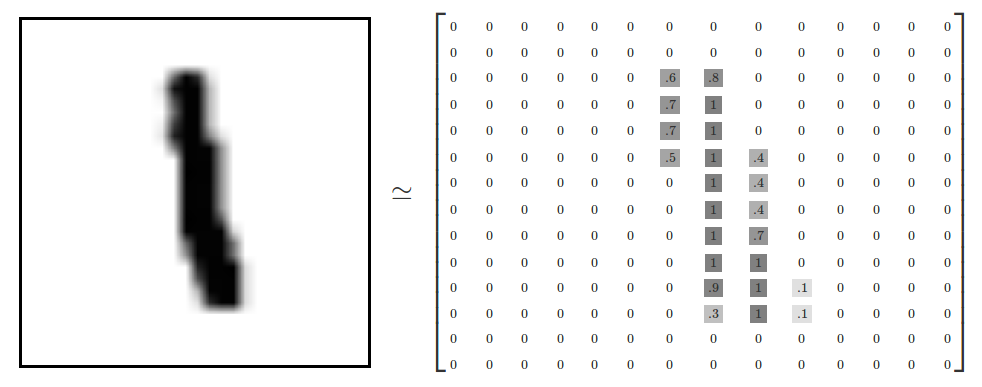
\includegraphics[width=.8\textwidth]{../SOURCE/images/MNIST-Matrix.png}
\caption{}
\end{figure}

Ⓔ \textcolor{etc}{We can flatten this array into a vector of $ 28 \times 28 = 784$ numbers. It doesn't matter how we flatten the array, as long as we're consistent between images. From this perspective, the MNIST images are just a bunch of points in a 784-dimensional vector space, with a \href{http://colah.github.io/posts/2014-10-Visualizing-MNIST/}{very rich structure} (warning: computationally intensive visualizations).}

Ⓒ 我们把这个数组展开成一个向量,长度是 $ 28 \times 28 = 784$.如何展开这个数组(数字间的顺序)不重要,只要保持各个图片采用相同的方式展开.从这个角度来看,MNIST数据集的图片就是在784维向量空间里面的点, 并且拥有比较\href{http://colah.github.io/posts/2014-10-Visualizing-MNIST/}{复杂的结构} (注意: 此类数据的可视化是计算密集型的).

Ⓔ \textcolor{etc}{Flattening the data throws away information about the 2D structure of the image. Isn't that bad? Well, the best computer vision methods do exploit this structure, and we will in later tutorials. But the simple method we will be using here, a softmax regression, won't.}

Ⓒ 展平图片的数字数组会丢失图片的二维结构信息.这显然是不理想的,最优秀的计算机视觉方法会挖掘并利用这些结构信息,我们会在后续教程中介绍.但是在这个教程中我们忽略这些结构,所介绍的简单数学模型,softmax回归(softmax regression),不会利用这些结构信息.

Ⓔ \textcolor{etc}{The result is that \lstinline{mnist.train.images} is a tensor (an n-dimensional array) with a shape of \lstinline{[55000, 784]}. The first dimension indexes the images and the second dimension indexes the pixels in each image. Each entry in the tensor is the pixel intensity between 0 and 1, for a particular pixel in a particular image.}

Ⓒ 因此,在MNIST训练数据集中,\lstinline{mnist.train.images}是一个形状为 \lstinline{[55000, 784]} 的张量,第一个维度数字用来索引图片,第二个维度数字用来索引每张图片中的像素点.在此张量里的每一个元素,都表示某张图片里的某个像素的强度值,值介于0和1之间.

\begin{figure}[htbp]
\centering
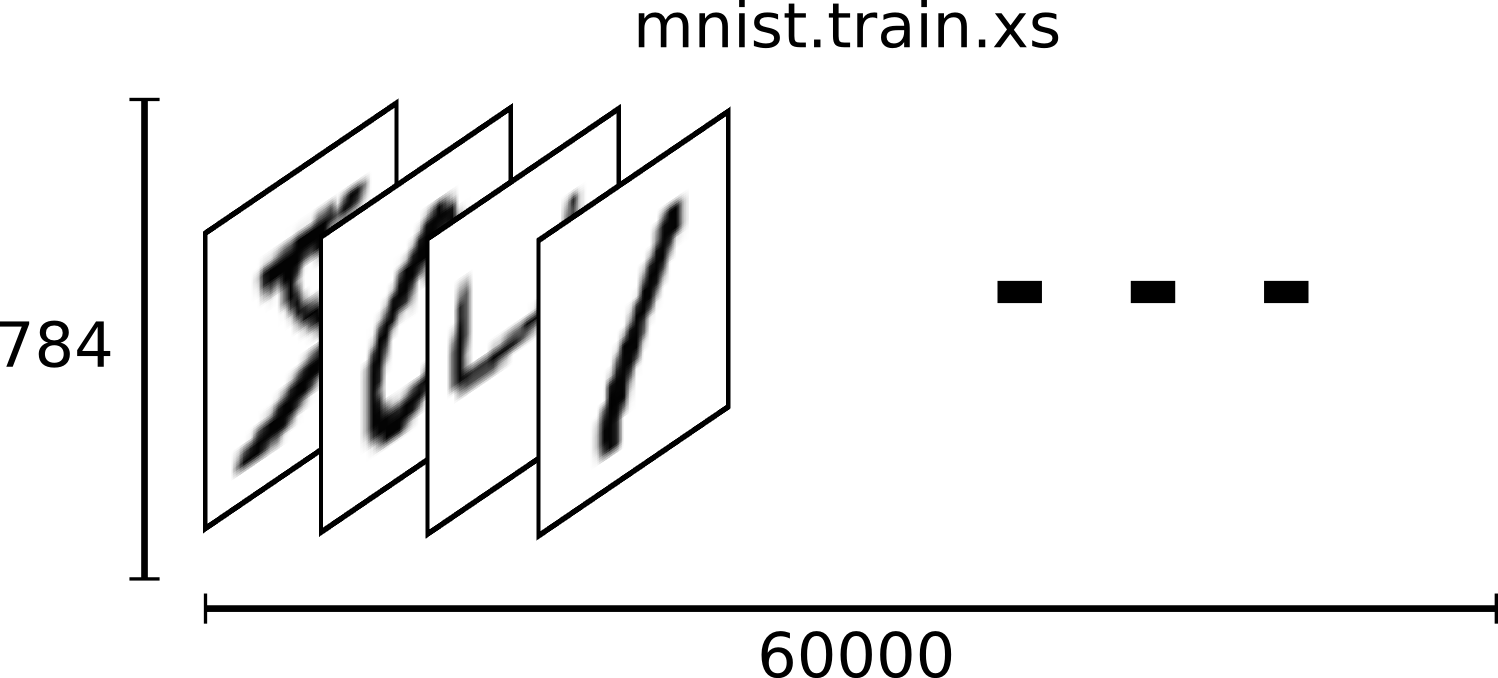
\includegraphics[width=.65\textwidth]{../SOURCE/images/mnist-train-xs.png}
\caption{}
\end{figure}

Ⓔ \textcolor{etc}{The corresponding labels in MNIST are numbers between 0 and 9, describing which digit a given image is of. For the purposes of this tutorial, we're going to want our labels as "one-hot vectors". A one-hot vector is a vector which is 0 in most dimensions, and 1 in a single dimension. In this case, the $n$th digit will be represented as a vector which is 1 in the $n$th dimensions. For example, 3 would be $[0,0,0,1,0,0,0,0,0,0]$. Consequently, \lstinline{mnist.train.labels} is a \lstinline{[55000, 10]} array of floats.}

Ⓒ 相对应的MNIST数据集的标签是介于0到9的数字,用来描述给定图片里表示的数字.为了用于这个教程,我们使标签数据是"one-hot vectors". 一个one-hot向量除了某一位的数字是1以外其余各维度数字都是0.所以在此教程中,数字n将表示成一个只有在第$n$维度(从0开始)数字为1的10维向量.比如,标签3将表示成(\lstinline{[0,0,0,1,0,0,0,0,0,0]}).因此,\lstinline{mnist.train.labels}是一个 \lstinline{[55000, 10]} 的数字矩阵.

\begin{figure}[htbp]
\centering
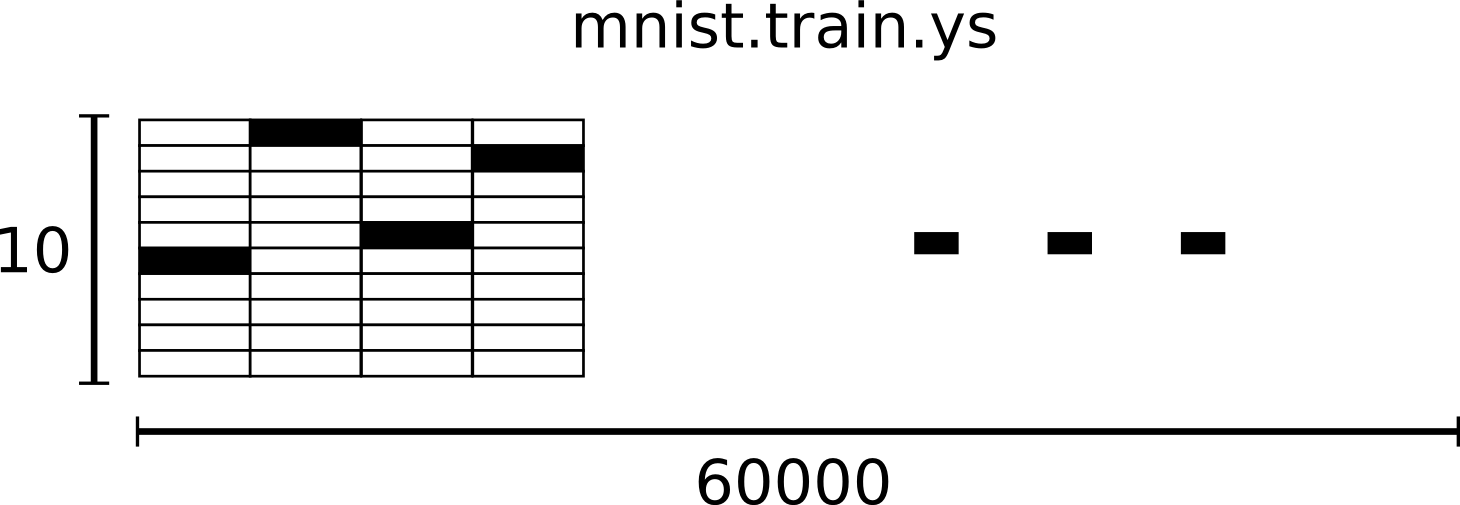
\includegraphics[width=.7\textwidth]{../SOURCE/images/mnist-train-ys.png}
\caption{}
\end{figure}

Ⓔ \textcolor{etc}{We're now ready to actually make our model!}

Ⓒ 现在,我们准备开始真正的建模之旅!

\subsection {Softmax回归介绍}

Ⓔ We know that every image in MNIST is a digit, whether it's a zero or a nine. We want to be able to look at an image and give probabilities for it being each digit. For example, our model might look at a picture of a nine and be 80\% sure it's a nine, but give a 5\% chance to it being an eight (because of the top loop) and a bit of probability to all the others because it isn't sure.

Ⓒ 我们知道MNIST数据集的每一张图片都表示一个(0到9的)数字.那么,如果模型若能看到一张图就能知道它属于各个数字的对应概率就好了。比如,我们的模型可能看到一张数字"9"的图片,就判断出它是数字"9"的概率为80\%,而有5\%的概率属于数字"8"(因为8和9都有上半部分的小圆),同时给予其他数字对应的小概率(因为该图像代表它们的可能性微乎其微).\index{Softmax regression}

Ⓔ This is a classic case where a softmax regression is a natural, simple model. If you want to assign probabilities to an object being one of several different things, softmax is the thing to do. Even later on, when we train more sophisticated models, the final step will be a layer of softmax.

Ⓒ 这是能够体现softmax回归自然简约的一个典型案例.softmax模型可以用来给不同的对象分配概率.在后文,我们训练更加复杂的模型时,最后一步也往往需要用softmax来分配概率.

Ⓔ A softmax regression has two steps: first we add up the evidence of our input being in certain classes, and then we convert that evidence into probabilities.

Ⓒ softmax回归(softmax regression)分两步:首先对输入被分类对象属于某个类的“证据”相加求和,然后将这个“证据”的和转化为概率.

Ⓔ To tally up the evidence that a given image is in a particular class, we do a weighted sum of the pixel intensities. The weight is negative if that pixel having a high intensity is evidence against the image being in that class, and positive if it is evidence in favor.

Ⓒ 我们使用加权的方法来累积计算一张图片是否属于某类的“证据”。如果图片的像素强有力的体现该图不属于某个类,则权重为负数,相反如果这个像素拥有有利的证据支持这张图片属于这个类,那么权值为正.

Ⓔ The following diagram shows the weights one model learned for each of these classes. Red represents negative weights, while blue represents positive weights.

Ⓒ 下面的图片显示了一个模型学习到的图片上每个像素对于特定数字类的权值.红色代表负权值,蓝色代表正权值.

\begin{figure}[htbp]
\centering
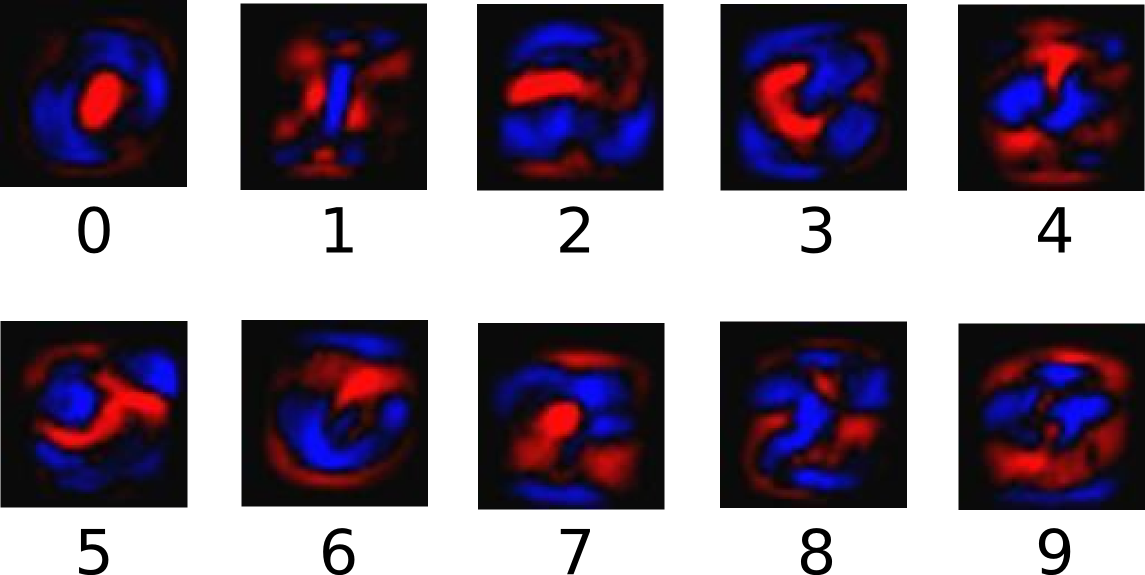
\includegraphics[width=.65\textwidth]{../SOURCE/images/softmax-weights.png}
\caption{}
\end{figure}

Ⓔ We also add some extra evidence called a bias. Basically, we want to be able to say that some things are more likely independent of the input. The result is that the evidence for a class $i$ given an input $x$ is:

Ⓒ 我们也需要引入额外的“证据”,可称之为偏置量(bias)。总的来说,我们希望它代表了与所输入向无关的判断证据.因此对于给定的输入图片$x$代表某数字$i$的总体证据可以表示为:
\begin{equation}
evidence_i = \sum_j{W_{i,j}}x_j+b_i
\end{equation}\\
Ⓔ where $W_i$ is the weights and $b_i$ is the bias for class $i$, and $j$ is an index for summing over the pixels in our input image $x$. We then convert the evidence tallies into our predicted probabilities y using the "softmax" function:\\
Ⓒ 其中,$W_i$ 代表权重,$b_i$ 代表第 $i$ 类的偏置量,$j$ 代表给定图片 $x$ 的像素索引用于像素求和.然后用softmax函数可以把这些证据转换成概率$y$:\\
\begin{equation}
y = softmax(evidence)
\end{equation}\\
Ⓔ Here softmax is serving as an "activation" or "link" function, shaping the output of our linear function into the form we want -- in this case, a probability distribution over 10 cases. You can think of it as converting tallies of evidence into probabilities of our input being in each class. It's defined as:\\
Ⓒ 这里的softmax可以看成是一个\emph{激励}(activation)函数或是\emph{链接}(link)函数,把我们定义的线性函数的输出转换成我们想要的格式,也就是关于10个数字类的概率分布.因此,给定一张图片,它对于每一个数字的吻合度可以被softmax函数转换成为一个概率值.softmax函数可以定义为:\\
\begin{equation}
softmax(x) = normalize(exp(x))
\end{equation}\\
Ⓔ If you expand that equation out, you get:\\
展开等式右边的子式,可以得到:\\
\begin{equation}
softmax(x)_i = \frac{exp(x_i)}{\sum_j{exp(x_j)}}
\end{equation}\\
Ⓔ But it's often more helpful to think of softmax the first way: exponentiating its inputs and then normalizing them. The exponentiation means that one more unit of evidence increases the weight given to any hypothesis multiplicatively. And conversely, having one less unit of evidence means that a hypothesis gets a fraction of its earlier weight. No hypothesis ever has zero or negative weight. Softmax then normalizes these weights, so that they add up to one, forming a valid probability distribution. (To get more intuition about the softmax function, check out the \href{http://neuralnetworksanddeeplearning.com/chap3.html#softmax}{section} on it in Michael Nieslen's book, complete with an interactive visualization.)\\
Ⓒ 但是更多的时候把softmax模型函数定义为第一种形式:把输入值当成幂指数求值,再正则化这些结果值.这个幂运算表示,更大的证据对应更大的假设模型(hypothesis)里面的乘数权重值.反之,拥有更少的证据意味着在假设模型里面拥有更小的乘数系数.假设模型里的权值不可以是0值或者负值.Softmax然后会正则化这些权重值,使它们的总和等于1,以此构造一个有效的概率分布.(更多的关于Softmax函数的信息,可以参考Michael Nieslen的书里面的\href{http://neuralnetworksanddeeplearning.com/chap3.html#softmax}{这个部分},其中有关于softmax的可交互式的可视化解释.)

Ⓔ You can picture our softmax regression as looking something like the following, although with a lot more $x$s. For each output, we compute a weighted sum of the $x$s, add a bias, and then apply softmax.\\
对于softmax回归模型可以用下面的图解释,对于输入的$xs$ 加权求和,再分别加上一个偏置量,最后再输入到softmax函数中:
\begin{center}
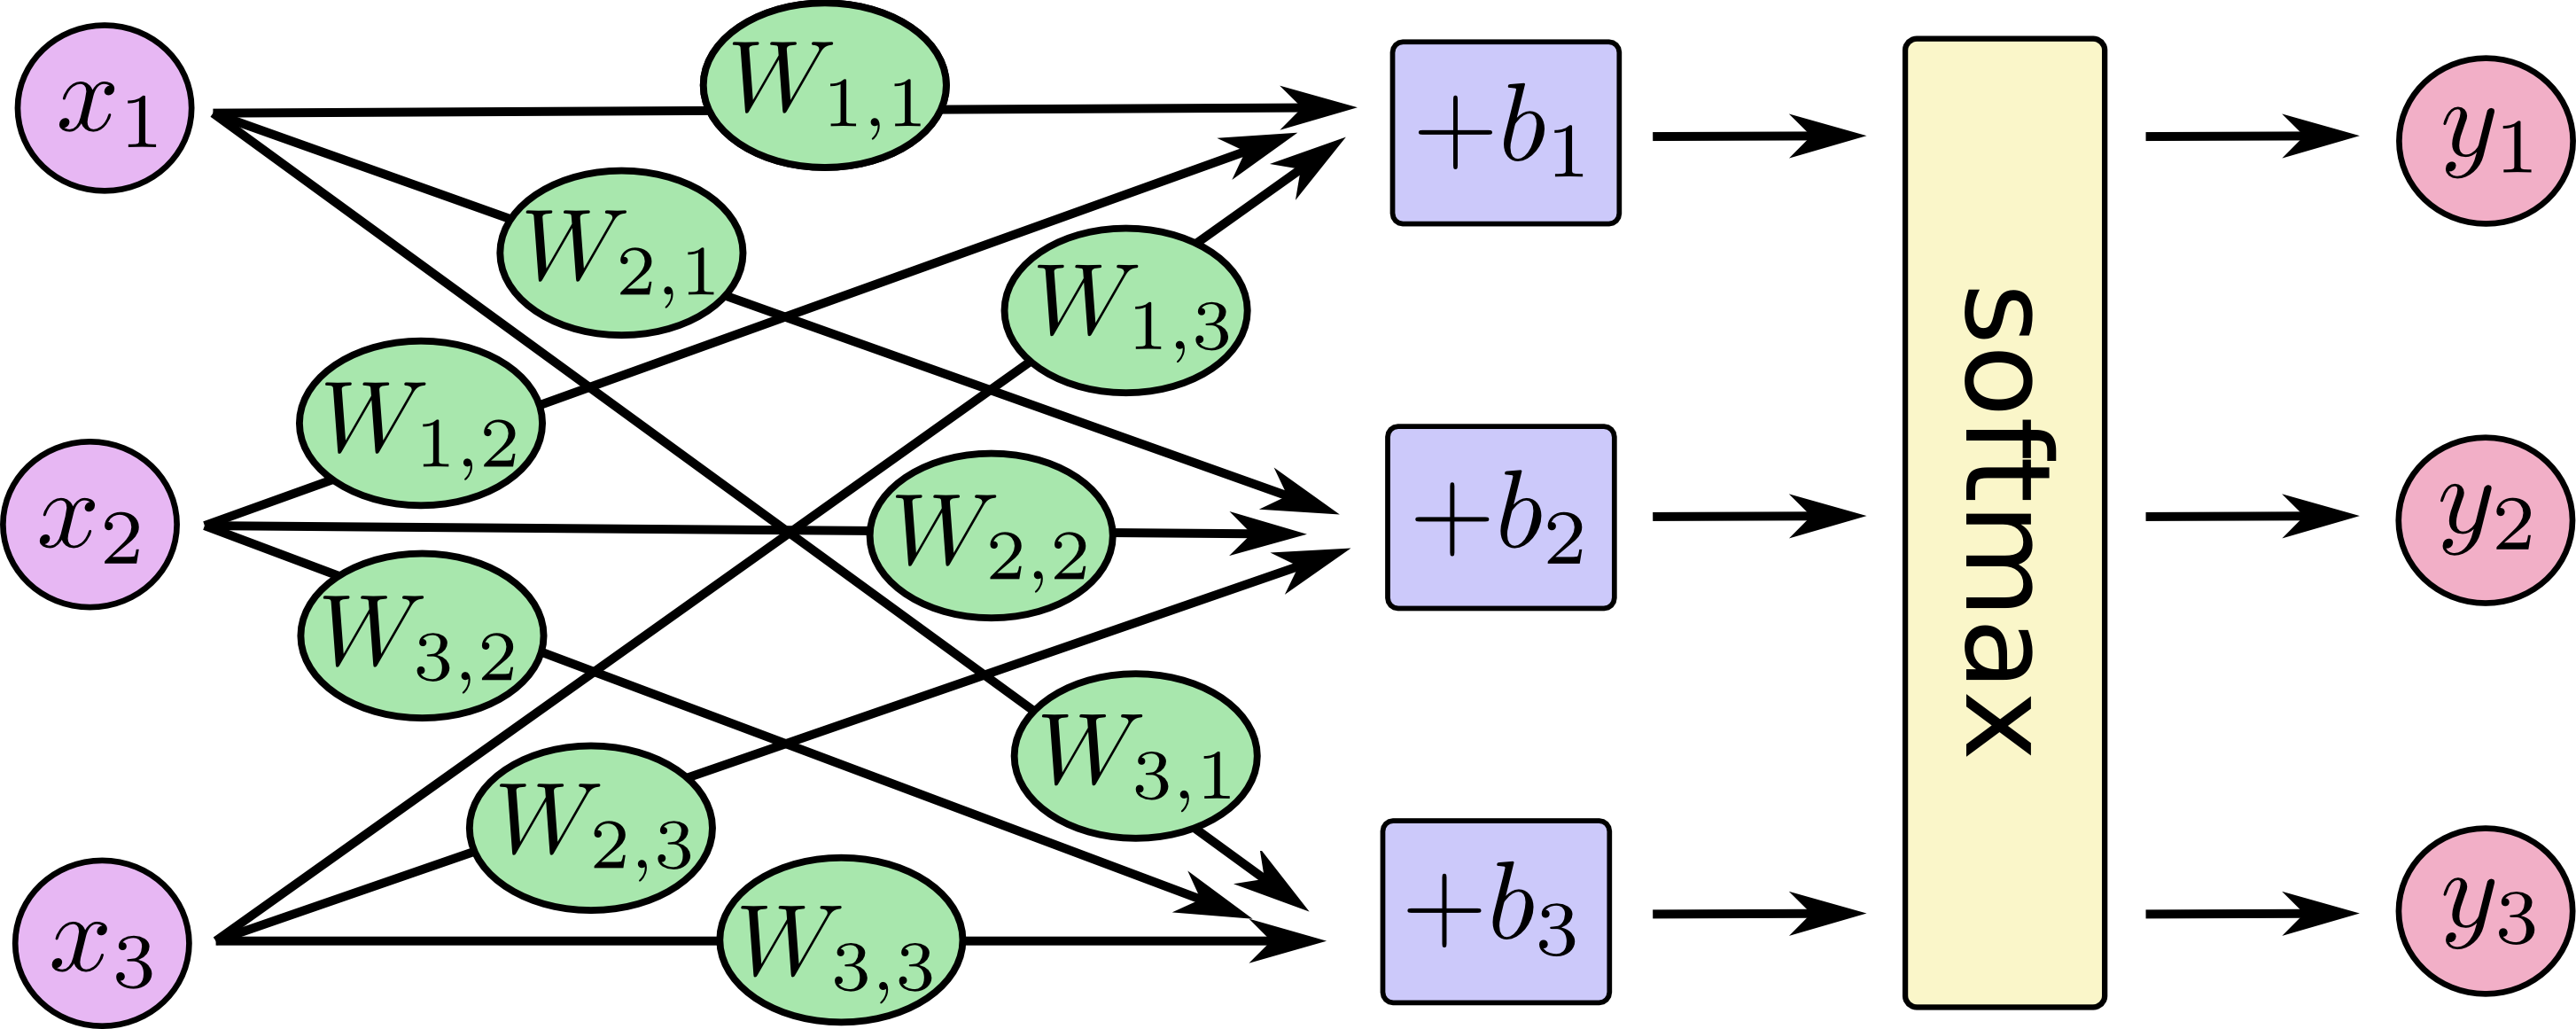
\includegraphics[width=.65\textwidth]{../SOURCE/images/softmax-regression-scalargraph.png}
\end{center}
Ⓔ If we write that out as equations, we get:\\
如果把它写成一个方程,可以得到:
\begin{center}
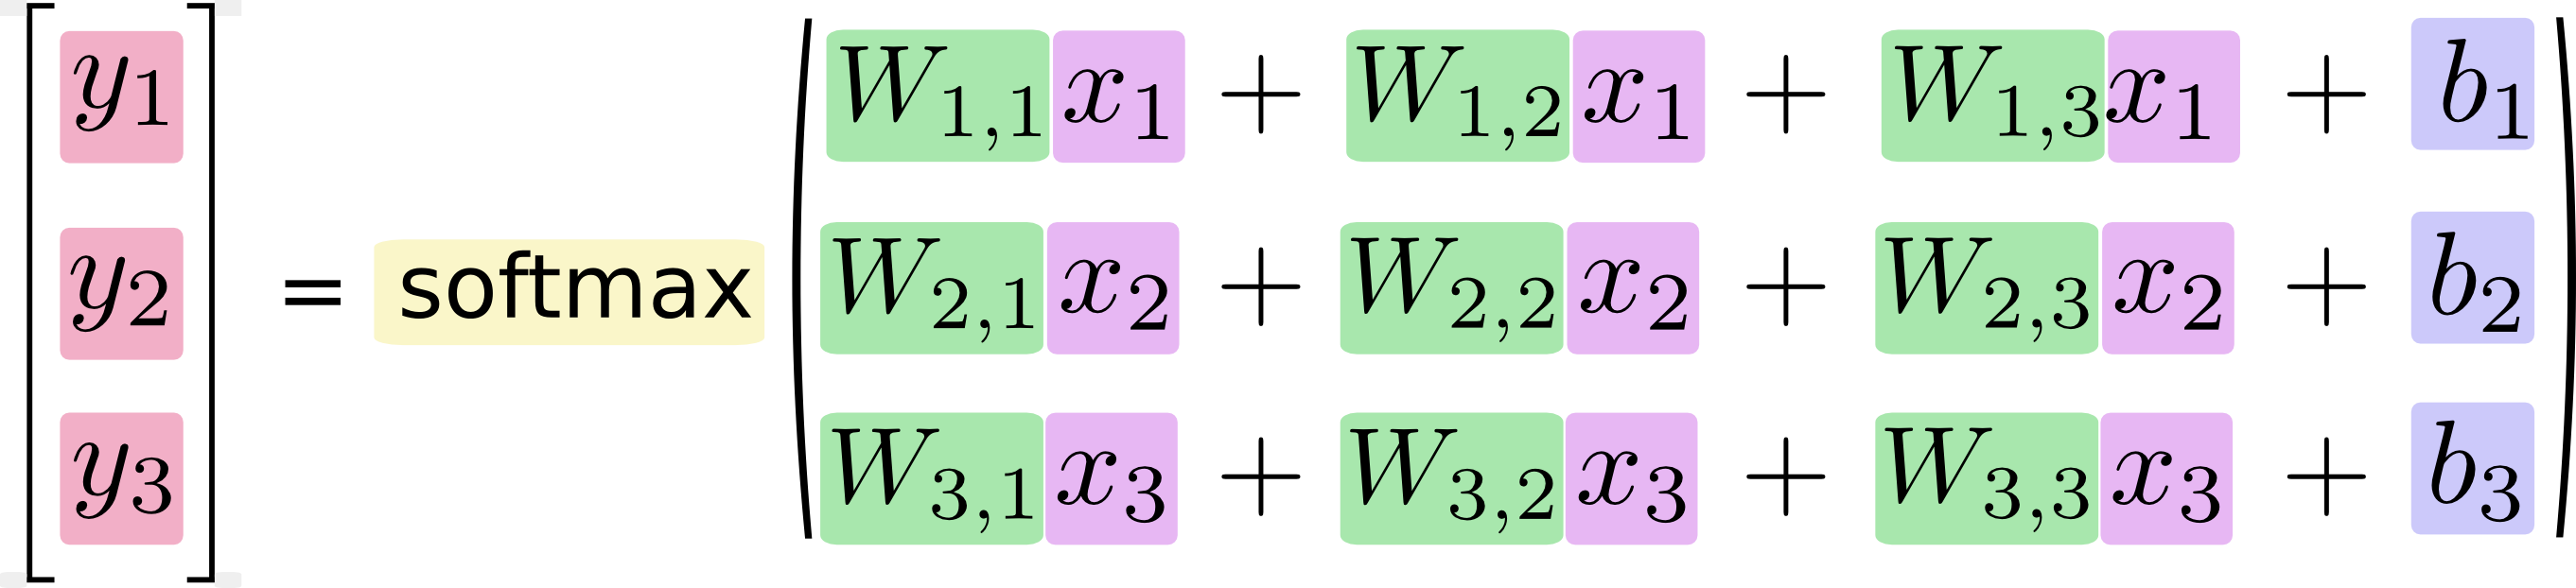
\includegraphics[width=.68\textwidth]{../SOURCE/images/softmax-regression-scalarequation.png}
\end{center}
Ⓔ We can "vectorize" this procedure, turning it into a matrix multiplication and vector addition. This is helpful for computational efficiency. (It's also a useful way to think.)\\
我们也可以用向量表示这个计算过程:用矩阵乘法和向量相加.这有助于提高计算效率(也是一种更有效的思考方式).
\begin{center}
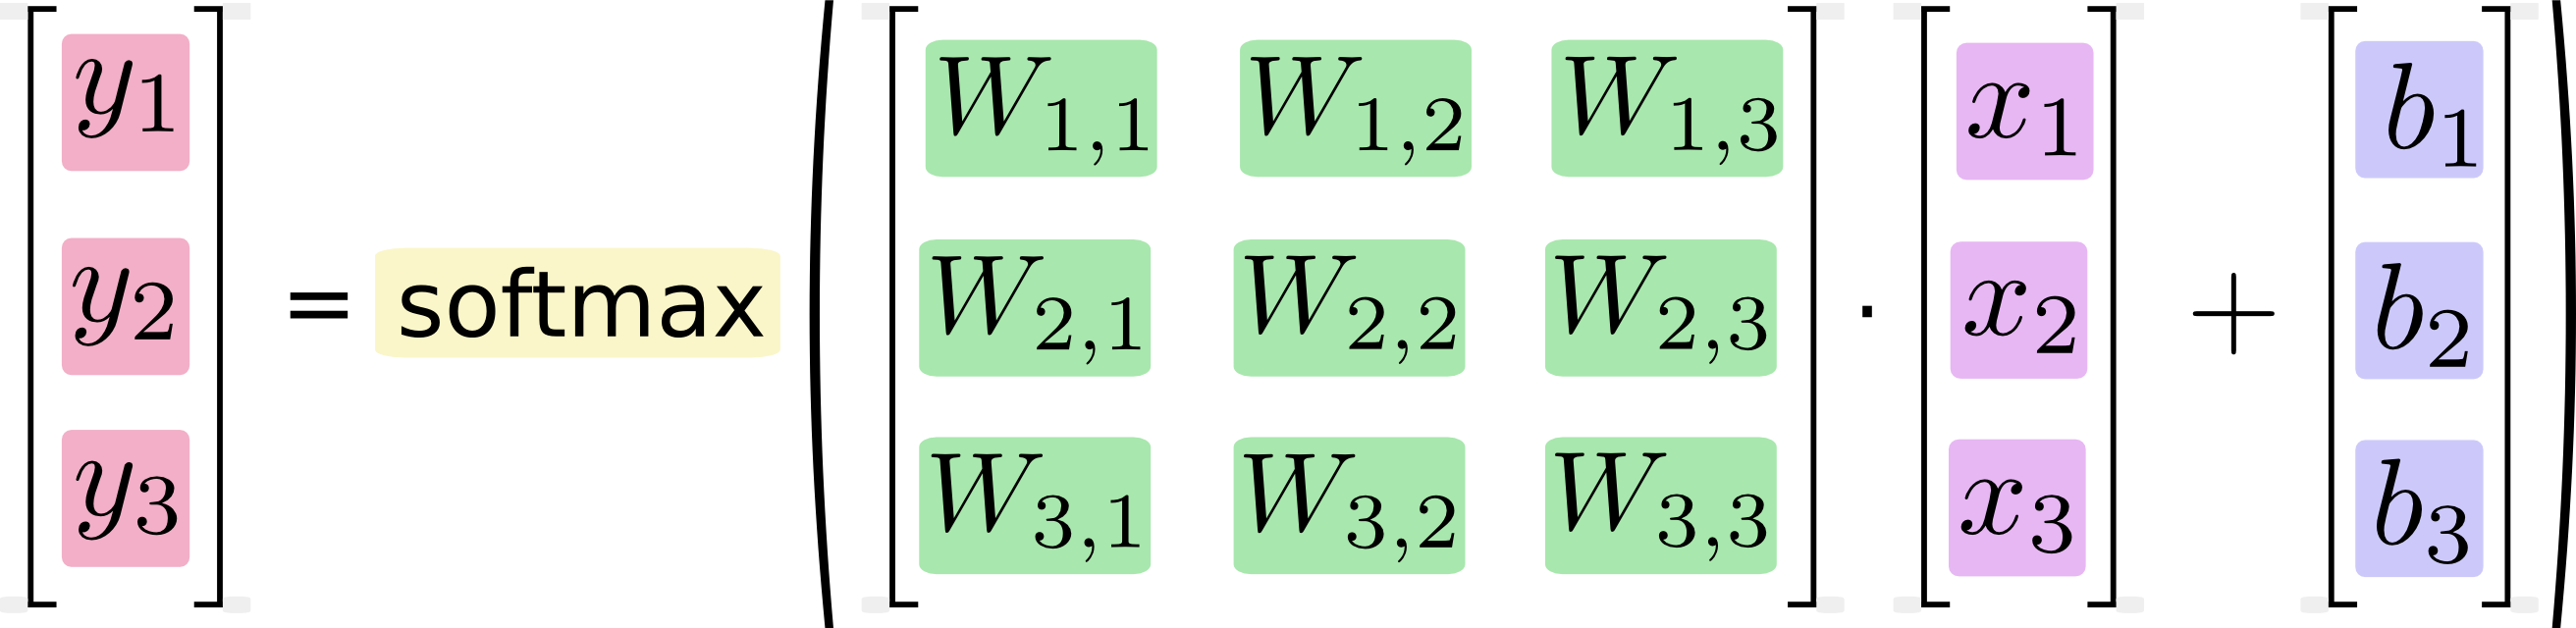
\includegraphics[width=.68\textwidth]{../SOURCE/images/softmax-regression-vectorequation.png}
\end{center}
Ⓔ More compactly, we can just write:\\
更进一步,可以写成更加紧凑的方式:
\begin{equation}
y = softmax(W_x+b)
\end{equation}

\subsection {实现回归模型}
Ⓔ To do efficient numerical computing in Python, we typically use libraries like NumPy that do expensive operations such as matrix multiplication outside Python, using highly efficient code implemented in another language. Unfortunately, there can still be a lot of overhead from switching back to Python every operation. This overhead is especially bad if you want to run computations on GPUs or in a distributed manner, where there can be a high cost to transferring data.

为了在python中高效的进行数值计算,我们通常会调用(如NumPy)外部函数库,把类似矩阵乘法这样的复杂运算使用其他外部语言实现.不幸的是,从外部计算切换回Python的每一个操作,仍然是一个很大的开销.如果你用GPU来进行外部计算,这样的开销会更大.用分布式的计算方式,也会花费更多的资源用来传输数据.

Ⓔ TensorFlow also does its heavy lifting outside python, but it takes things a step further to avoid this overhead. Instead of running a single expensive operation independently from Python, TensorFlow lets us describe a graph of interacting operations that run entirely outside Python. (Approaches like this can be seen in a few machine learning libraries.)

TensorFlow也把复杂的计算放在python之外完成,但是为了避免前面说的那些开销,它做了进一步完善.TensorFlow不单独地运行单一的复杂计算,而是让我们可以先用图描述一系列可交互的计算操作,然后全部一起在Python之外运行.(这样类似的运行方式,可以在不少的机器学习库中看到.)


Ⓔ To use TensorFlow, we need to import it.

使用TensorFlow之前,首先导入它:

\begin{lstlisting}
import tensorflow as tf
\end{lstlisting}

Ⓔ We describe these interacting operations by manipulating symbolic variables. Let's create one:

我们通过操作符号变量来描述这些可交互的操作单元,可以用下面的方式创建一个:

\begin{lstlisting}
x = tf.placeholder("float", [None, 784])
\end{lstlisting}\\
Ⓔ \lstinline{x} isn't a specific value. It's a \lstinline{placeholder}, a value that we'll input when we ask TensorFlow to run a computation. We want to be able to input any number of MNIST images, each flattened into a 784-dimensional vector. We represent this as a 2-D tensor of floating-point numbers, with a shape \lstinline{[None, 784]}. (Here None means that a dimension can be of any length.)\\
\lstinline{x} 不是一个特定的值,而是一个占位符\lstinline{placeholder},我们在TensorFlow运行计算时输入这个值.我们希望能够输入任意数量的MNIST图像,每一张图展平成784维的向量.我们用2维的浮点数张量来表示这些图,这个张量的形状是 [None,784].(这里的\lstinline{None}表示此张量的第一个维度可以是任何长度的.)


Ⓔ We also need the weights and biases for our model. We could imagine treating these like additional inputs, but TensorFlow has an even better way to handle it: \lstinline{Variable}. A \lstinline{Variable} is a modifiable tensor that lives in TensorFlow's graph of interacting operations. It can be used and even modified by the computation. For machine learning applications, one generally has the model parameters be \lstinline{Variables}.

我们的模型也需要权重值和偏置量,当然我们可以把它们当做是另外的输入(使用占位符),但TensorFlow有一个更好的方法来表示它们:\lstinline{Variable}. 一个\lstinline{Variable}代表一个可修改的张量,存在在TensorFlow的用于描述交互性操作的图中.它们可以用于计算输入值,也可以在计算中被修改.对于各种机器学习应用,一般都会有模型参数,可以用\lstinline{Variable}表示.

\begin{lstlisting}
W = tf.Variable(tf.zeros([784,10]))
b = tf.Variable(tf.zeros([10]))
\end{lstlisting}

Ⓔ We create these \lstinline{Variables} by giving \lstinline{tf.Variable} the initial value of the \lstinline{Variable}: in this case, we initialize both W and b as tensors full of zeros. Since we are going to learn \lstinline{W} and \lstinline{b}, it doesn't matter very much what they initially are.

我们赋予\lstinline{tf.Variable} 不同的初值来创建不同的\lstinline{Variable}:在这里,我们都用全为零的张量来初始化\lstinline{W}和\lstinline{b}.因为我们要学习\lstinline{W}和\lstinline{b}的值,它们的初值可以随意设置.


Ⓔ Notice that W has a shape of \lstinline{[784, 10]} because we want to multiply the 784-dimensional image vectors by it to produce 10-dimensional vectors of evidence for the difference classes. \lstinline{b} has a shape of \lstinline{[10]} so we can add it to the output.


注意,\lstinline{W}的维度是\lstinline{[784,10]},因为我们想要用784维的图片向量乘以它以得到一个10维的证据值向量,每一位对应不同数字类.\lstinline{b}的形状是\lstinline{[10]},所以我们可以直接把它加到输出上面.

Ⓔ We can now implement our model. It only takes one line!

现在,可以实现我们的模型了,只需以下一行代码:

\begin{lstlisting}
y = tf.nn.softmax(tf.matmul(x,W) + b)
\end{lstlisting}

Ⓔ First, we multiply $x$ by $W$ with the expression \lstinline{tf.matmul(x, W)}. This is flipped from when we multiplied them in our equation, where we had $W_x$, as a small trick to deal with x being a 2D tensor with multiple inputs. We then add b, and finally apply \lstinline{tf.nn.softmax}.

首先,我们用\lstinline{tf.matmul(X,W)}表示$x$乘以$W$,对应之前等式里面的$W_x$,这里$x$是一个2维张量拥有多个输入.然后再加上$b$,把和输入到\lstinline{tf.nn.softmax}函数里面.

Ⓔ That's it. It only took us one line to define our model, after a couple short lines of setup. That isn't because TensorFlow is designed to make a softmax regression particularly easy: it's just a very flexible way to describe many kinds of numerical computations, from machine learning models to physics simulations. And once defined, our model can be run on different devices: your computer's CPU, GPUs, and even phones!

至此,我们先用了几行简短的代码来设置变量,然后只用了一行代码来定义我们的模型.TensorFlow不仅仅可以使softmax回归模型计算变得特别简单,它也用这种非常灵活的方式来描述其他各种数值计算,从机器学习模型对物理学模拟仿真模型.一旦被定义好之后,我们的模型就可以在不同的设备上运行:计算机的CPU,GPU,甚至是手机!

\subsection{训练模型}

Ⓔ In order to train our model, we need to define what it means for the model to be good. Well, actually, in machine learning we typically define what it means for a model to be bad, called the cost or loss, and then try to minimize how bad it is. But the two are equivalent.

为了训练我们的模型,我们首先需要定义一个指标来评估这个模型是好的.其实,在机器学习,我们通常定义指标来表示一个模型是坏的,这个指标称为成本(cost)或损失(loss),然后尽量最小化这个指标.但是,这两种方式是相同的.

Ⓔ One very common, very nice cost function is "cross-entropy." Surprisingly, cross-entropy arises from thinking about information compressing codes in information theory but it winds up being an important idea in lots of areas, from gambling to machine learning. It's defined:\\
一个非常常见的,非常漂亮的成本函数是“交叉熵”(cross-entropy).交叉熵产生于信息论里面的信息压缩编码技术,但是它后来演变成为从博弈论到机器学习等其他领域里的重要技术手段.它的定义如下:
\\
\begin{equation}
H_{y'}(y) = -\sum_i{y_{i}'log(y_i)}
\end{equation}
\\
Ⓔ where $y$ is our predicted probability distribution, and $y'$ is the true distribution (the one-hot vector we'll input). In some rough sense, the cross-entropy is measuring how inefficient our predictions are for describing the truth. Going into more detail about cross-entropy is beyond the scope of this tutorial, but it's well worth \href{http://colah.github.io/posts/2015-09-Visual-Information/}{understanding}.
\\
$y$是我们预测的概率分布,$y'$是实际的分布(我们输入的one-hot vector).比较粗糙的理解是,交叉熵是用来衡量我们的预测用于描述真相的低效性.更详细的关于交叉熵的解释超出本教程的范畴,但是你很有必要好好\href{http://colah.github.io/posts/2015-09-Visual-Information/}{理解}它.

Ⓔ To implement cross-entropy we need to first add a new placeholder to input the correct answers:\\
为了计算交叉熵,我们首先需要添加一个新的占位符用于输入正确值:
\\
\begin{lstlisting}
y = tf.placeholder("float", [None,10])
\end{lstlisting}
Ⓔ Then we can implement the cross-entropy $-\sum{y'log(y)}$,\\
然后我们可以用 $-\sum{y'log(y)}$ 计算交叉熵:

\begin{lstlisting}
cross_entropy = -tf.reduce_sum(y_*tf.log(y))
\end{lstlisting}

Ⓔ First, \lstinline{tf.log} computes the logarithm of each element of \lstinline{y.} Next, we multiply each element of \lstinline{y_} with the corresponding element of \lstinline{tf.log(y)}. Finally, \lstinline{tf.reduce_sum} adds all the elements of the tensor.

首先,用 \lstinline{tf.log} 计算y的每个元素的对数.接下来,我们把\lstinline{y_}的每一个元素和\lstinline{tf.log(y_)}的对应元素相乘.最后,用\lstinline{tf.reduce_sum}计算张量的所有元素的总和.

Ⓔ Note that this isn't just the cross-entropy of the truth with a single prediction, but the sum of the cross-entropies for all the images we looked at. In this example, we have 100 images in each batch: how well we are doing on 100 data points is a much better description of how good our model is than a single data point.

值得注意的是,这里的交叉熵不仅仅用来衡量单一的一对预测和真实值,而是所有100幅图片的交叉熵的总和.对于100个数据点的预测表现比单一数据点的表现能更好地描述我们的模型的性能.

Ⓔ Now that we know what we want our model to do, it's very easy to have TensorFlow train it to do so. Because TensorFlow knows the entire graph of your computations, it can automatically use the \href{http://colah.github.io/posts/2015-08-Backprop/}{backpropagation algorithm} to efficiently determine how your variables affect the cost you ask it minimize. Then it can apply your choice of optimization algorithm to modify the variables and reduce the cost.

现在我们知道我们需要我们的模型做什么啦,用TensorFlow来训练它是非常容易的.因为TensorFlow拥有一张描述你各个计算单元的图,它可以自动地使用\href{http://colah.github.io/posts/2015-08-Backprop/}{反向传播算法(backpropagation algorithm)}来有效地确定你的变量是如何影响你想要最小化的那个成本值的.然后,TensorFlow会用你选择的优化算法来不断地修改变量以降低成本.

\begin{lstlisting}
train_step = tf.train.GradientDescentOptimizer(0.01).minimize(cross_entropy)
\end{lstlisting}

Ⓔ In this case, we ask TensorFlow to minimize \lstinline{cross_entropy} using the gradient descent algorithm with a learning rate of $0.01$. Gradient descent is a simple procedure, where TensorFlow simply shifts each variable a little bit in the direction that reduces the cost. But TensorFlow also provides \href{https://www.tensorflow.org/versions/master/api_docs/python/train.html#optimizers}{many other optimization algorithms}: using one is as simple as tweaking one line.

在这里,我们要求TensorFlow用梯度下降算法(gradient descent algorithm)以0.01的学习速率最小化交叉熵.梯度下降算法(gradient descent algorithm)是一个简单的学习过程,TensorFlow只需将每个变量一点点地往使成本不断降低的方向移动.当然TensorFlow也提供了\href{https://www.tensorflow.org/versions/master/api_docs/python/train.html#optimizers}{其他许多优化算法}:只要简单地调整一行代码就可以使用其他的算法.\index{梯度下降法}

Ⓔ What TensorFlow actually does here, behind the scenes, is it adds new operations to your graph which implement backpropagation and gradient descent. Then it gives you back a single operation which, when run, will do a step of gradient descent training, slightly tweaking your variables to reduce the cost.

TensorFlow在这里实际上所做的是,它会在后台给描述你的计算的那张图里面增加一系列新的计算操作单元用于实现反向传播算法和梯度下降算法.然后,它返回给你的只是一个单一的操作,当运行这个操作时,它用梯度下降算法训练你的模型,微调你的变量,不断减少成本.

Ⓔ Now we have our model set up to train. One last thing before we launch it, we have to add an operation to initialize the variables we created:

现在,我们已经设置好了我们的模型.在运行计算之前,我们需要添加一个操作来初始化我们创建的变量:

\begin{lstlisting}
init = tf.initialize_all_variables()
\end{lstlisting}
\\
Ⓔ We can now launch the model in a \lstinline{Session}, and run the operation that initializes the variables:\\
现在我们可以在一个 \lstinline{Session} 里面启动我们的模型,并且初始化变量:
\begin{lstlisting}
sess = tf.Session()
sess.run(init)
\end{lstlisting}
\\
Ⓔ Let's train -- we'll run the training step 1000 times!\\
然后开始训练模型,这里我们让模型循环训练1000次!
\begin{lstlisting}
for i in range(1000):
    batch_xs, batch_ys = mnist.train.next_batch(100)
    sess.run(train_step, feed_dict={x: batch_xs, y_: batch_ys})
\end{lstlisting}

Ⓔ Each step of the loop, we get a "batch" of one hundred random data points from our training set. We run \lstinline{train_step} feeding in the batches data to replace the placeholders.

该循环的每个步骤中,我们都会随机抓取训练数据中的100个批处理数据点,然后我们用这些数据点作为参数替换之前的占位符来运行\lstinline{train_step}.

Ⓔ Using small batches of random data is called stochastic training -- in this case, stochastic gradient descent. Ideally, we'd like to use all our data for every step of training because that would give us a better sense of what we should be doing, but that's expensive. So, instead, we use a different subset every time. Doing this is cheap and has much of the same benefit.

使用一小部分的随机数据来进行训练被称为随机训练(stochastic training)---在这里更确切的说是随机梯度下降训练.理想情况下,我们希望用我们所有的数据来进行每一步的训练,因为这能给我们更好的训练结果,但显然这需要很大的计算开销.所以,每一次训练我们可以使用不同的数据子集,这样做既可以减少计算开销,又可以最大化地学习到数据集的总体特性.

\subsection{Evaluating Our Model   ||   评估我们的模型}

Ⓔ How well does our model do?

那么我们的模型性能如何呢?

Ⓔ Well, first let's figure out where we predicted the correct label. \lstinline{tf.argmax} is an extremely useful function which gives you the index of the highest entry in a tensor along some axis. For example, \lstinline{tf.argmax(y,1)} is the label our model thinks is most likely for each input, while \lstinline{tf.argmax(y_,1)} is the correct label. We can use \lstinline{tf.equal} to check if our prediction matches the truth.

首先让我们找出那些预测正确的标签.\lstinline{tf.argmax()}是一个非常有用的函数,它能给你在一个张量里沿着某条轴的最高条目的索引值.比如,\lstinline{tf.argmax(y,1)}是模型认为每个输入最有可能对应的那些标签,而\lstinline{tf.argmax(y_,1)}代表正确的标签.我们可以用\lstinline{tf.equal} 来检测我们的预测是否真实标签匹配.

\begin{lstlisting}
correct_prediction = tf.equal(tf.argmax(y,1), tf.argmax(y_,1))
\end{lstlisting}

Ⓔ That gives us a list of booleans. To determine what fraction are correct, we cast to floating point numbers and then take the mean. For example, \lstinline{[True, False, True, True]} would become \lstinline{[1,0,1,1]} which would become $0.75$.

这行代码会给我们一组布尔值.为了确定正确预测项的比例,我们可以把布尔值转换成浮点数,然后取平均值.例如,\lstinline{[True, False, True, True]}会变成\lstinline{[1,0,1,1]},取平均值后得到 $0.75$ .

\begin{lstlisting}
accuracy = tf.reduce_mean(tf.cast(correct_prediction, "float"))
\end{lstlisting}

Ⓔ Finally, we ask for our accuracy on our test data.

最后,我们计算所学习到的模型在测试数据集上面的正确率.

\begin{lstlisting}
print sess.run(accuracy, feed_dict={x: mnist.test.images, y_: mnist.test.labels})
\end{lstlisting}

Ⓔ This should be about 91\%.

最终结果值应该大约是91\%.

Ⓔ Is that good? Well, not really. In fact, it's pretty bad. This is because we're using a very simple model. With some small changes, we can get to 97\%/. The best models can get to over 99.7\% accuracy! (For more information, have a look at this \href{http://rodrigob.github.io/are_we_there_yet/build/classification_datasets_results.html}{list of results})

这个结果好吗?嗯,并不太好.事实上,这个结果是很差的.这是因为我们仅仅使用了一个非常简单的模型.不过,做一些小小的改进,我们就可以得到97\%的正确率.最好的模型甚至可以获得超过99.7\%的准确率!(想了解更多信息,请参考这个\href{http://rodrigob.github.io/are_we_there_yet/build/classification_datasets_results.html}{结果对比列表}.)

Ⓔ What matter is that we learned from this model. Still, if you're feeling a bit down about these results, check out the next tutorial where we do a lot better, and learn how to build more sophisticated models using TensorFlow!

比结果更重要的是,我们从这个模型中学习到的设计思想.不过,如果你仍然对这里的结果有点失望,可以查看下个教程,在那里你将学到如何用TensorFlow构建更加复杂的模型以获得更好的性能!

原文地址:\href{http://tensorflow.org/tutorials/mnist/beginners/index.md}{MNIST For ML Beginners}

%!TEX program = xelatex
% Encoding: UTF8
% SEIKA 2015


% Chapter 2 Tutorials
% Section 2.3 minist_pros


\newpage
\section {深入MNIST} \label{MINIST_pros}
TensorFlow是一个做大规模数值计算的强大库。其中一个特点就是它能够实现和训练深度神经网络。 在这一小节里,我们将会学习在MNIST上构建深度卷积分类器的基本步骤。

\emph{这个教程假设你已经熟悉神经网络和MNIST数据集。如果你尚未了解,请查看\hyperref[MINIST_beginner]{新手指南}.}

\subsection {安装}
在创建模型之前,我们会先加载MNIST数据集,然后启动一个TensorFlow的session。

\subsubsection {加载MINIST数据}

为了方便起见,我们已经准备了一个脚本来自动下载和导入MNIST数据集。它会自动创建一个'MNIST\_data'的目录来存储数据。

\begin{lstlisting}
import input_data
mnist = input_data.read_data_sets('MNIST_data', one_hot=True)
\end{lstlisting}

\subsubsection {开始TensorFlow的交互会话}

Tensorflow基于一个高效的C++模块进行运算。与这个模块的连接叫做session。一般而言,使用TensorFlow程序的流程是先创建一个图,然后在session中加载它。

这里,我们使用更加方便的InteractiveSession类。通过它,你可以更加灵活地构建你的代码。它能让你在运行图的时候,插入一些构建计算图的操作。这能给使用交互式文本shell如iPython带来便利。如果你没有使用InteractiveSession的话,你需要在开始session和加载图之前,构建整个计算图。

\begin{lstlisting}
import tensorflow as tf
sess = tf.InteractiveSession()
\end{lstlisting}

\subsubsection {计算图}

传统的计算行为中,为了更高效地在Python里进行数值计算,我们一般会使用像NumPy这样用其他语言编写的lib,在Python外完成这些费时的操作(例如矩阵运算)。可是,每一步操作依然会经常在Python和第三方lib之间切换。这些操作很糟糕,特别是当你想在GPU上进行计算,又或者想使用分布式的做法的时候。这些情况下数据传输代价高昂。

在TensorFlow中,也有Python与外界的频繁操作。但是它在这一方面,做了进一步的改良。TensorFlow构建一个交互操作的图,作为一个整体在Python外运行,而不是以代价高昂的单个交互操为单位在Python外运行。这与Theano、Torch的做法很相似。

所以,这部分Python代码,目的是构建这个在外部运行的计算图,并安排这个计算图的哪一部分应该被运行。详细请阅读计算图 部分的基本用法。 %add link here

\subsection{构建Softmax Regression模型}

在这小节里,我们将会构建一个一层线性的softmax regression模型。下一节里,我们会扩展到多层卷积网络。

\subsubsection{占位符(placeholder)}
我们先来创建计算图的输入(图片)和输出(类别)。

\begin{lstlisting}
x = tf.placeholder("float", shape=[None, 784])
y_ = tf.placeholder("float", shape=[None, 10])
\end{lstlisting}

这里的\lstinline{x}和\lstinline{y}并不是具体值,他们是一个\lstinline{placeholder},是一个变量,在TensorFlow运行计算的时候使用。

输入图片x是浮点数2维张量。这里,定义它的\lstinline{shape}为\lstinline{[None, 784]},其中784是单张展开的MNIST图片的维度数。\lstinline{shape}的第一维输入指代一个batch的大小,\lstinline{None},可为任意值。输出值\lstinline{y_}也是一个2维张量,其中每一行为一个10维向量代表对应MNIST图片的分类。

虽然\lstinline{placeholder}的\lstinline{shape}参数是可选的,但有了它,TensorFlow能够自动捕捉因数据维度不一致导致的错误。

\subsubsection{变量(Variables)}

我们现在为模型定义权重\lstinline{W}和偏置\lstinline{b}。它们可以被视作是额外的输入量,但是TensorFlow有一个更好的方式来处理:\lstinline{Variable}。一个\lstinline{Variable}代表着在TensorFlow计算图中的一个值,它是能在计算过程中被读取和修改的。在机器学习的应用过程中,模型参数一般用\lstinline{Variable}来表示。

\begin{lstlisting}
W = tf.Variable(tf.zeros([784,10]))
b = tf.Variable(tf.zeros([10]))
\end{lstlisting}

我们在调用\lstinline{tf.Variable}的时候传入初始值。在这个例子里,我们把\lstinline{W}和\lstinline{b}都初始化为零向量。\lstinline{W}是一个$784\times10$的矩阵(因为我们有784个特征和10个输出值)。\lstinline{b}是一个10维的向量(因为我们有10个分类)。

\lstinline{Variable}需要在\lstinline{session}之前初始化,才能在\lstinline{session}中使用。初始化需要初始值(本例当中是全为零)传入并赋值给每一个\lstinline{Variable}。这个操作可以一次性完成。

\begin{lstlisting}
sess.run(tf.initialize_all_variables())
\end{lstlisting}

\subsubsection{预测分类与损失函数}
现在我们可以实现我们的regression模型了。这只需要一行!我们把图片\lstinline{x}和权重矩阵\lstinline{W}相乘,加上偏置\lstinline{b},然后计算每个分类的softmax概率值。

\begin{lstlisting}
y = tf.nn.softmax(tf.matmul(x,W) + b)
\end{lstlisting}

在训练中最小化损失函数同样很简单。我们这里的损失函数用目标分类和模型预测分类之间的交叉熵。

\begin{lstlisting}
cross_entropy = -tf.reduce_sum(y_*tf.log(y))
\end{lstlisting}

注意,\lstinline{tf.reduce_sum}把\lstinline{minibatch}里的每张图片的交叉熵值都加起来了。我们计算的交叉熵是指整个\lstinline{minibatch}的。

\subsection{训练模型}

我们已经定义好了模型和训练的时候用的损失函数,接下来使用TensorFlow来训练。因为TensorFlow知道整个计算图,它会用自动微分法来找到损失函数对于各个变量的梯度。TensorFlow有大量内置的优化算法 这个例子中,我们用最速下降法让交叉熵下降,步长为0.01。

\begin{lstlisting}
train_step = tf.train.GradientDescentOptimizer(0.01).minimize(cross_entropy)
\end{lstlisting}

这一行代码实际上是用来往计算图上添加一个新操作,其中包括计算梯度,计算每个参数的步长变化,并且计算出新的参数值。

\lstinline{train_step}这个操作,用梯度下降来更新权值。因此,整个模型的训练可以通过反复地运行\lstinline{train_step}来完成。

\begin{lstlisting}
for i in range(1000):
    batch = mnist.train.next_batch(50)
    train_step.run(feed_dict={x: batch[0], y_: batch[1]})
\end{lstlisting}

每一步迭代,我们都会加载50个训练样本,然后执行一次train\_step,使用feed\_dict,用训练数据替换placeholder向量x和y\_。

注意,在计算图中,你可以用feed\_dict来替代任何张量,并不仅限于替换placeholder。

\subsubsection{评估模型}

我们的模型效果怎样?

首先,要先知道我们哪些label是预测正确了。tf.argmax是一个非常有用的函数。它会返回一个张量某个维度中的最大值的索引。例如,tf.argmax(y,1)表示我们模型对每个输入的最大概率分类的分类值。而 tf.argmax(y\_,1)表示真实分类值。我们可以用tf.equal来判断我们的预测是否与真实分类一致。

\begin{lstlisting}
correct_prediction = tf.equal(tf.argmax(y,1), tf.argmax(y_,1))
\end{lstlisting}

这里返回一个布尔数组。为了计算我们分类的准确率,我们将布尔值转换为浮点数来代表对、错,然后取平均值。例如:[True, False, True, True]变为[1,0,1,1],计算出平均值为0.75。

\begin{lstlisting}
accuracy = tf.reduce_mean(tf.cast(correct_prediction, "float"))
\end{lstlisting}

最后,我们可以计算出在测试数据上的准确率,大概是91\%。

\begin{lstlisting}
print accuracy.eval(feed_dict={x: mnist.test.images, y_: mnist.test.labels})
\end{lstlisting}

\subsection{构建多层卷积网络模型}

在MNIST上只有91\%正确率,实在太糟糕。在这个小节里,我们用一个稍微复杂的模型:卷积神经网络来改善效果。这会达到大概99.2\%的准确率。虽然不是最高,但是还是比较让人满意。

\subsubsection{权重初始化}

在创建模型之前,我们先来创建权重和偏置。一般来说,初始化时应加入轻微噪声,来打破对称性,防止零梯度的问题。因为我们用的是ReLU,所以用稍大于0的值来初始化偏置能够避免节点输出恒为0的问题(dead neurons)。为了不在建立模型的时候反复做初始化操作,我们定义两个函数用于初始化。

\begin{lstlisting}
def weight_variable(shape):
    initial = tf.truncated_normal(shape, stddev=0.1)
    return tf.Variable(initial)

def bias_variable(shape):
    initial = tf.constant(0.1, shape=shape)
    return tf.Variable(initial)
\end{lstlisting}

\subsubsection{卷积和池化}

TensorFlow在卷积和池化上有很强的灵活性。我们怎么处理边界?步长应该设多大?在这个实例里,我们会一直使用vanilla版本。我们的卷积使用1步长(stride size),0边距(padding size)的模板,保证输出和输入是同一个大小。我们的池化用简单传统的2x2大小的模板做max pooling。为了代码更简洁,我们把这部分抽象成一个函数。

\begin{lstlisting}
def conv2d(x, W):
    return tf.nn.conv2d(x, W, strides=[1, 1, 1, 1], padding='SAME')

def max_pool_2x2(x):
    return tf.nn.max_pool(x, ksize=[1, 2, 2, 1], strides=[1, 2, 2, 1], padding='SAME')
\end{lstlisting}

\subsubsection{第一层卷积}

现在我们可以开始实现第一层了。它由一个卷积接一个max pooling完成。卷积在每个$5\times5$的patch中算出32个特征。权重是一个\lstinline{[5, 5, 1, 32]}的张量,前两个维度是patch的大小,接着是输入的通道数目,最后是输出的通道数目。输出对应一个同样大小的偏置向量。

\begin{lstlisting}
W_conv1 = weight_variable([5, 5, 1, 32])
b_conv1 = bias_variable([32])
\end{lstlisting}

为了用这一层,我们把x变成一个4d向量,第2、3维对应图片的宽高,最后一维代表颜色通道。

\begin{lstlisting}
x_image = tf.reshape(x, [-1,28,28,1])
\end{lstlisting}

我们把x\_image和权值向量进行卷积相乘,加上偏置,使用ReLU激活函数,最后max pooling。

\begin{lstlisting}
h_conv1 = tf.nn.relu(conv2d(x_image, W_conv1) + b_conv1)
h_pool1 = max_pool_2x2(h_conv1)
\end{lstlisting}

\subsubsection{第二层卷积}

为了构建一个更深的网络,我们会把几个类似的层堆叠起来。第二层中,每个5x5的patch会得到64个特征。

\begin{lstlisting}
W_conv2 = weight_variable([5, 5, 32, 64])
b_conv2 = bias_variable([64])

h_conv2 = tf.nn.relu(conv2d(h_pool1, W_conv2) + b_conv2)
h_pool2 = max_pool_2x2(h_conv2)
\end{lstlisting}

\subsubsection{密集连接层}

现在,图片降维到$7\times7$,我们加入一个有1024个神经元的全连接层,用于处理整个图片。我们把池化层输出的张量reshape成一些向量,乘上权重矩阵,加上偏置,使用ReLU激活。

\begin{lstlisting}
W_fc1 = weight_variable([7 * 7 * 64, 1024])
b_fc1 = bias_variable([1024])

h_pool2_flat = tf.reshape(h_pool2, [-1, 7*7*64])
h_fc1 = tf.nn.relu(tf.matmul(h_pool2_flat, W_fc1) + b_fc1)
\end{lstlisting}

\textbf{Dropout}

为了减少过拟合,我们在输出层之前加入dropout。我们用一个placeholder来代表一个神经元在dropout中被保留的概率。这样我们可以在训练过程中启用dropout,在测试过程中关闭dropout。 TensorFlow的\lstinline{tf.nn.dropout}操作会自动处理神经元输出值的scale。所以用dropout的时候可以不用考虑scale。

\begin{lstlisting}
keep_prob = tf.placeholder("float")
h_fc1_drop = tf.nn.dropout(h_fc1, keep_prob)
\end{lstlisting}

\subsubsection{输出层}

最后,我们添加一个softmax层,就像前面的单层softmax regression一样。

\begin{lstlisting}
W_fc2 = weight_variable([1024, 10])
b_fc2 = bias_variable([10])

y_conv=tf.nn.softmax(tf.matmul(h_fc1_drop, W_fc2) + b_fc2)
\end{lstlisting}

\subsubsection{训练和评估模型}

这次效果又有多好呢?我们用前面几乎一样的代码来测测看。只是我们会用更加复杂的ADAM优化器来做梯度最速下降,在feed\_dict中加入额外的参数keep\_prob来控制dropout比例。然后每100次迭代输出一次日志。

\begin{lstlisting}
cross_entropy = -tf.reduce_sum(y_*tf.log(y_conv))
train_step = tf.train.AdamOptimizer(1e-4).minimize(cross_entropy)
correct_prediction = tf.equal(tf.argmax(y_conv,1), tf.argmax(y_,1))
accuracy = tf.reduce_mean(tf.cast(correct_prediction, "float"))
sess.run(tf.initialize_all_variables())
for i in range(20000):
  batch = mnist.train.next_batch(50)
  if i%100 == 0:
    train_accuracy = accuracy.eval(feed_dict={
        x:batch[0], y_: batch[1], keep_prob: 1.0})
    print "step %d, training accuracy %g"%(i, train_accuracy)
  train_step.run(feed_dict={x: batch[0], y_: batch[1], keep_prob: 0.5})

print "test accuracy %g"%accuracy.eval(feed_dict={
    x: mnist.test.images, y_: mnist.test.labels, keep_prob: 1.0})
\end{lstlisting}

以上代码,在最终测试集上的准确率大概是99.2\%。

目前为止,我们已经学会了用TensorFlow来快速和简易地搭建、训练和评估一个复杂一点儿的深度学习模型。

原文地址:Deep MNIST for Experts
翻译:chenweican
校对:HongyangWang
%!TEX program = xelatex
% Encoding: UTF8
% SEIKA 2015


% Chapter 2 Tutorials
% Section 2.4 TensorFlow Mechanics 101


\newpage
\section {TensorFlow Mechanics 101} \label{tf_mech101}

Ⓔ \textcolor{etc}{\textbf{Code}: \href{https://tensorflow/g3doc/tutorials/mnist/}{tensorflow/examples/tutorials/mnist/}}

\textbf{代码地址}: \href{https://tensorflow/g3doc/tutorials/mnist/}{tensorflow/g3doc/tutorials/mnist/}

Ⓔ \textcolor{etc}{The goal of this tutorial is to show how to use TensorFlow to train and evaluate a simple feed-forward neural network for handwritten digit classification using the (classic) MNIST data set. The intended audience for this tutorial is experienced machine learning users interested in using TensorFlow.}

本篇教程的目的,是向大家展示如何利用TensorFlow使用(经典)MNIST数据集训练并评估一个用于识别手写数字的简易前馈神经网络(feed-forward neural network)。我们的目标读者是有兴趣使用TensorFlow的机器学习资深人士。

Ⓔ \textcolor{etc}{These tutorials are not intended for teaching Machine Learning in general.}

因此,撰写该系列教程并不是为了教大家机器学习领域的基础知识。

Ⓔ \textcolor{etc}{Please ensure you have followed the instructions to \href{https://www.tensorflow.org/versions/master/get_started/os_setup.html}{install TensorFlow}.}

在学习本教程之前,请确保您已按照安装TensorFlow教程中的要求,完成了\href{https://www.tensorflow.org/versions/master/get_started/os_setup.html}{安装}。

\subsection {教程使用的文件} \label{minist_tf}

本教程引用如下文件:

% add table here

只需要直接运行fully\_connected\_feed.py文件,就可以开始训练:

python fully\_connected\_feed.py

\subsection {准备数据}

MNIST是机器学习领域的一个经典问题,指的是让机器查看一系列大小为$28\times28$像素的手写数字灰度图像,并判断这些图像代表0--9中的哪一个数字。

\begin{figure}[htbp]
\centering

\includegraphics[width=.55\textwidth]{../SOURCE/images/MNIST.png}
\caption{}
\end{figure}

更多相关信息,请查阅Yann LeCun网站中关于MNIST的介绍 或者Chris Olah对MNIST的可视化探索。

\subsubsection{下载}

在\lstinline{run\_training()}方法的一开始,\lstinline{input\_data.read\_data\_sets()}函数会确保你的本地训练文件夹中,已经下载了正确的数据,然后将这些数据解压并返回一个含有\lstinline{DataSet}实例的字典。

\begin{lstlisting}
data_sets = input_data.read_data_sets(FLAGS.train_dir, FLAGS.fake_data)
\end{lstlisting}\footnote{\lstinline{fake_data}标记是用于单元测试的,读者可以不必理会。}

% 数据集 | 目的
% --- | ---
% `data_sets.train` | 55000个图像和标签(labels),作为主要训练集。
% `data_sets.validation` | 5000个图像和标签,用于迭代验证训练准确度。
% `data_sets.test` | 10000个图像和标签,用于最终测试训练准确度(trained accuracy)。

Add table here\footnote{了解更多数据有关信息,请查阅此系列教程的[数据下载](mnist/download/index.md)
部分.}

\subsubsection{输入与占位符}
% ### 输入与占位符(Inputs and Placeholders) <a class="md-anchor" id="AUTOGENERATED-inputs-and-placeholders"></a>

\lstinline{placeholder_inputs()}函数将生成两个\lstinline{tf.placeholder}
%[`tf.placeholder`](../api_docs/python/io_ops.md#placeholder)
操作,定义传入图表中的shape参数,shape参数中包括\lstinline{batch_size}值,后续还会将实际的训练用例传入图表。

\begin{lstlisting}
images_placeholder = tf.placeholder(tf.float32, shape=(batch_size, IMAGE_PIXELS))
labels_placeholder = tf.placeholder(tf.int32, shape=(batch_size))
\end{lstlisting}

在训练循环(training loop)的后续步骤中,传入的整个图像和标签数据集会被切片,以符合每一个操作所设置的 \lstinline{batch_size}值,占位符操作将会填补以符合这个\lstinline{batch_size}值。然后使用\lstinline{feed_dict}参数,将数据传入\lstinline{sess.run()}函数。

\subsection {构建图表 (Build the Graph)}
%## 构建图表 (Build the Graph)<a class="md-anchor" id="AUTOGENERATED-build-the-graph"></a>

在为数据创建占位符之后,就可以运行\lstinline{mnist.py}文件,经过三阶段的模式函数操作:\lstinline{inference()}, \lstinline{loss()\lstinline},和\lstinline{training()}。图表就构建完成了。

\begin{enumerate}

\item \lstinline{inference()} —— 尽可能地构建好图表,满足促使神经网络向前反馈并做出预测的要求。

\item \lstinline{loss()} —— 往inference图表中添加生成损失(loss)所需要的操作(ops)。

\item \lstinline{training()} —— 往损失图表中添加计算并应用梯度(gradients)所需的操作。
\end{enumerate}

\begin{figure}[htbp]
\centering
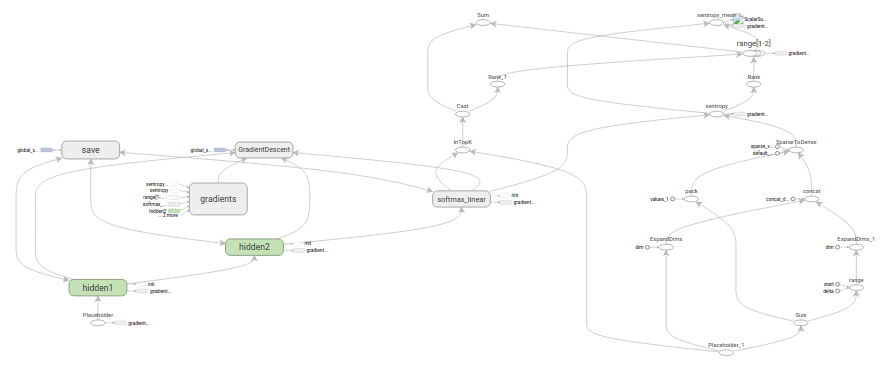
\includegraphics[width=.95\textwidth]{../SOURCE/images/mnist_subgraph.png}
\caption{}
\end{figure}

\subsubsection{推理(Inference)}
%### 推理(Inference) <a class="md-anchor" id="AUTOGENERATED-inference"></a>

\lstinline{inference()}函数会尽可能地构建图表,做到返回包含了预测结果(output prediction)的Tensor。

它接受图像占位符为输入,在此基础上借助ReLu(Rectified Linear Units)激活函数,构建一对完全连接层(layers),以及一个有着十个节点(node)、指明了输出logtis模型的线性层。

每一层都创建于一个唯一的\lstinline{tf.name_scope}%(../api_docs/python/framework.md#name_scope)
之下,创建于该作用域之下的所有元素都将带有其前缀。

\begin{lstlisting}
with tf.name_scope('hidden1') as scope:
\end{lstlisting}

在定义的作用域中,每一层所使用的权重和偏差都在\lstinline{tf.Variable}
%(../api_docs/python/state_ops.md#Variable)
实例中生成,并且包含了各自期望的shape。

\begin{lstlisting}
weights = tf.Variable(tf.truncated_normal([IMAGE_PIXELS, hidden1_units], stddev=1.0 / math.sqrt(float(IMAGE_PIXELS))), name='weights')
biases = tf.Variable(tf.zeros([hidden1_units]), name='biases')
\end{lstlisting}

例如,当这些层是在\lstinline{hidden1}作用域下生成时,赋予权重变量的独特名称将会是"\lstinline{hidden1/weights}"。

每个变量在构建时,都会获得初始化操作(initializer ops)。

在这种最常见的情况下,通过\lstinline{tf.truncated_normal}
%(../api_docs/python/constant_op.md#truncated_normal)
函数初始化权重变量,给赋予的shape则是一个二维tensor,其中第一个维度代表该层中权重变量所连接(connect from)的单元数量,第二个维度代表该层中权重变量所连接到的(connect to)单元数量。对于名叫\lstinline{hidden1}的第一层,相应的维度则是\lstinline{[IMAGE_PIXELS, hidden1_units]},因为权重变量将图像输入连接到了\lstinline{hidden1}层。\lstinline{tf.truncated_normal}初始函数将根据所得到的均值和标准差,生成一个随机分布。

然后,通过\lstinline{tf.zeros}
%(../api_docs/python/constant_op.md#zeros)
函数初始化偏差变量(biases),确保所有偏差的起始值都是0,而它们的shape则是其在该层中所接到的(connect to)单元数量。

图表的三个主要操作,分别是两个\lstinline{tf.nn.relu}
%(../api_docs/python/nn.md#relu)
操作,它们中嵌入了隐藏层所需的\lstinline{tf.matmul}
%(../api_docs/python/math_ops.md#matmul)
;以及logits模型所需的另外一个\lstinline{tf.matmul}。三者依次生成,各自的\lstinline{tf.Variable}实例则与输入占位符或下一层的输出tensor所连接。

\begin{lstlisting}
hidden1 = tf.nn.relu(tf.matmul(images, weights) + biases)
\end{lstlisting}

\begin{lstlisting}
hidden2 = tf.nn.relu(tf.matmul(hidden1, weights) + biases)
\end{lstlisting}

\begin{lstlisting}
logits = tf.matmul(hidden2, weights) + biases
\end{lstlisting}

最后,程序会返回包含了输出结果的`logits`Tensor。

\subsubsection{损失(Loss)}

\lstinline{loss()}函数通过添加所需的损失操作,进一步构建图表。

首先,\lstinline{labels_placeholer}中的值,将被编码为一个含有1-hot values的Tensor。例如,如果类标识符为“3”,那么该值就会被转换为:
\lstinline{[0, 0, 0, 1, 0, 0, 0, 0, 0, 0]}

\begin{lstlisting}
batch_size = tf.size(labels)
labels = tf.expand_dims(labels, 1)
indices = tf.expand_dims(tf.range(0, batch_size, 1), 1)
concated = tf.concat(1, [indices, labels])
onehot_labels = tf.sparse_to_dense(
    concated, tf.pack([batch_size, NUM_CLASSES]), 1.0, 0.0)
\end{lstlisting}

之后,又添加一个\lstinline{tf.nn.softmax_cross_entropy_with_logits}
%`](../api_docs/python/nn.md#softmax_cross_entropy_with_logits)
操作\footnote{交叉熵是信息理论中的概念,可以让我们描述如果基于已有事实,相信神经网络所做的推测最坏会导致什么结果。更多详情,请查阅博文《可视化信息理论》(http://colah.github.io/posts/2015-09-Visual-Information/)},用来比较\lstinline{inference()}函数与1-hot标签所输出的logits Tensor。

\begin{lstlisting}
cross_entropy = tf.nn.softmax_cross_entropy_with_logits(logits, onehot_labels, name='xentropy')
\end{lstlisting}

然后,使用\lstinline{tf.reduce_mean}
%(../api_docs/python/math_ops.md#reduce_mean)
函数,计算batch维度(第一维度)下交叉熵(cross entropy)的平均值,将将该值作为总损失。

\begin{lstlisting}
loss = tf.reduce_mean(cross_entropy, name='xentropy_mean')
\end{lstlisting}

最后,程序会返回包含了损失值的Tensor。

\subsubsection{训练}

\lstinline{training()}函数添加了通过梯度下降(gradient descent)将损失最小化所需的操作。

首先,该函数从\lstinline{loss()}函数中获取损失Tensor,将其交给\lstinline{[tf.scalar_summary]}
% ](../api_docs/python/train.md#scalar_summary)
,后者在与\lstinline{SummaryWriter}(见下文)配合使用时,可以向事件文件(events file)中生成汇总值(summary values)。在本篇教程中,每次写入汇总值时,它都会释放损失Tensor的当前值(snapshot value)。

\begin{lstlisting}
tf.scalar_summary(loss.op.name, loss)
\end{lstlisting}

接下来,我们实例化一个\lstinline{[tf.train.GradientDescentOptimizer]}
% (../api_docs/python/train.md#GradientDescentOptimizer)
,负责按照所要求的学习效率(learning rate)应用梯度下降法(gradients)。

\begin{lstlisting}
optimizer = tf.train.GradientDescentOptimizer(FLAGS.learning_rate)
\end{lstlisting}

之后,我们生成一个变量用于保存全局训练步骤(global training step)的数值,并使用\lstinline{minimize()}
% (../api_docs/python/train.md#Optimizer.minimize)
函数更新系统中的三角权重(triangle weights)、增加全局步骤的操作。根据惯例,这个操作被称为\lstinline{train_op},是TensorFlow会话(session)诱发一个完整训练步骤所必须运行的操作(见下文)。

\begin{lstlisting}
global_step = tf.Variable(0, name='global_step', trainable=False)
train_op = optimizer.minimize(loss, global_step=global_step)
\end{lstlisting}

最后,程序返回包含了训练操作(training op)输出结果的Tensor。

\subsection{训练模型}

一旦图表构建完毕,就通过\lstinline{fully_connected_feed.py}文件中的用户代码进行循环地迭代式训练和评估。

\subsubsection{图表 (The Graph)}

在\lstinline{run_training()}这个函数的一开始,是一个Python语言中的\lstinline{with}命令,这个命令表明所有已经构建的操作都要与默认的\lstinline{[`tf.Graph`]}
%(../api_docs/python/framework.md#Graph)
全局实例关联起来。

\begin{lstlisting}
with tf.Graph().as_default():
\end{lstlisting}

\lstinline{tf.Graph}实例是一系列可以作为整体执行的操作。TensorFlow的大部分场景只需要依赖默认图表一个实例即可。

利用多个图表的更加复杂的使用场景也是可能的,但是超出了本教程的范围。

\subsubsection{会话 (The Session)}

完成全部的构建准备、生成全部所需的操作之后,我们就可以创建一个\lstinline{tf.Session}
%(../api_docs/python/client.md#Session)
,用于运行图表。

\begin{lstlisting}
sess = tf.Session()
\end{lstlisting}

另外,也可以利用\lstinline{with}代码块生成\lstinline{Session},限制作用域:

\begin{lstlisting}
with tf.Session() as sess:
\end{lstlisting}

\lstinline{Session}函数中没有传入参数,表明该代码将会依附于(如果还没有创建会话,则会创建新的会话)默认的本地会话。

生成会话之后,所有\lstinline{tf.Variable}实例都会立即通过调用各自初始化操作中的\lstinline{sess.run()}
%(../api_docs/python/client.md#Session.run)
函数进行初始化。

\begin{lstlisting}
init = tf.initialize_all_variables()
sess.run(init)
\end{lstlisting}

\lstinline{sess.run()}
%(../api_docs/python/client.md#Session.run)
方法将会运行图表中与作为参数传入的操作相对应的完整子集。在初次调用时,\lstinline{init}操作只包含了变量初始化程序\lstinline{tf.group}
%(../api_docs/python/control_flow_ops.md#group)
。图表的其他部分不会在这里,而是在下面的训练循环运行。

\subsubsection{训练循环}

完成会话中变量的初始化之后,就可以开始训练了。

训练的每一步都是通过用户代码控制,而能实现有效训练的最简单循环就是:

\begin{lstlisting}
for step in xrange(max_steps):
    sess.run(train_op)
\end{lstlisting}

但是,本教程中的例子要更为复杂一点,原因是我们必须把输入的数据根据每一步的情况进行切分,以匹配之前生成的占位符。

\paragragh{向图表提}

执行每一步时,我们的代码会生成一个反馈字典(feed dictionary),其中包含对应步骤中训练所要使用的例子,这些例子的哈希键就是其所代表的占位符操作。

\lstinline{fill_feed_dict}函数会查询给定的\lstinline{DataSet},索要下一批次\lstinline{batch_size}的图像和标签,与占位符相匹配的Tensor则会包含下一批次的图像和标签。

\begin{lstlisting}
images_feed, labels_feed = data_set.next_batch(FLAGS.batch_size)
\end{lstlisting}

然后,以占位符为哈希键,创建一个Python字典对象,键值则是其代表的反馈Tensor。

\begin{lstlisting}
feed_dict = {
    images_placeholder: images_feed,
    labels_placeholder: labels_feed,
}
\end{lstlisting}

这个字典随后作为\lstinline{feed_dict}参数,传入\lstinline{sess.run()}函数中,为这一步的训练提供输入样例。

\paragragh{检查状态}

在运行\lstinline{sess.run()}函数时,要在代码中明确其需要获取的两个值:\lstinline{[train_op, loss]}。

\begin{lstlisting}
for step in xrange(FLAGS.max_steps):
    feed_dict = fill_feed_dict(data_sets.train, images_placeholder, labels_placeholder)
    _, loss_value = sess.run([train_op, loss], feed_dict=feed_dict)
\end{lstlisting}

因为要获取这两个值,\lstinline{sess.run()}会返回一个有两个元素的元组。其中每一个\lstinline{Tensor}对象,对应了返回的元组中的numpy数组,而这些数组中包含了当前这步训练中对应Tensor的值。由于\lstinline{train_op}并不会产生输出,其在返回的元祖中的对应元素就是\lstinline{None},所以会被抛弃。但是,如果模型在训练中出现偏差,\lstinline{loss} Tensor的值可能会变成\lstinline{NaN},所以我们要获取它的值,并记录下来。

假设训练一切正常,没有出现\lstinline{NaN},训练循环会每隔100个训练步骤,就打印一行简单的状态文本,告知用户当前的训练状态。

\begin{lstlisting}
if step % 100 == 0:
    print 'Step %d: loss = %.2f (%.3f sec)' % (step, loss_value, duration)
\end{lstlisting}

\paragraph{状态可视化}
为了释放\lstinline{[TensorBoard]}
%(../how_tos/summaries_and_tensorboard.md)
所使用的事件文件(events file),所有的即时数据(在这里只有一个)都要在图表构建阶段合并至一个操作(op)中。

\begin{lstlisting}
summary_op = tf.merge_all_summaries()
\end{lstlisting}

在创建好会话(session)之后,可以实例化一个\lstinline{tf.train.SummaryWriter}
% (../api_docs/python/train.md#SummaryWriter)
,用于写入包含了图表本身和即时数据具体值的事件文件。

\begin{lstlisting}
summary_writer = tf.train.SummaryWriter(FLAGS.train_dir, graph_def=sess.graph_def)
\end{lstlisting}

最后,每次运行\lstinline{summary_op}时,都会往事件文件中写入最新的即时数据,函数的输出会传入事件文件读写器(writer)的\lstinline{add_summary()}函数。。

\begin{lstlisting}
summary_str = sess.run(summary_op, feed_dict=feed_dict)
summary_writer.add_summary(summary_str, step)
\end{lstlisting}

事件文件写入完毕之后,可以就训练文件夹打开一个TensorBoard,查看即时数据的情况。

\begin{figure}[htbp]
\centering
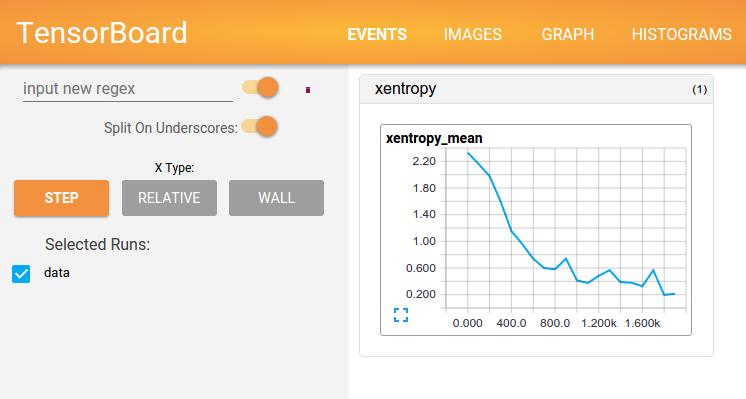
\includegraphics[width=.85\textwidth]{../SOURCE/images/mnist_tensorboard.png}
\centering
\end{figure}

% ![MNIST TensorBoard](../images/mnist_tensorboard.png "MNIST TensorBoard")

**注意**:了解更多如何构建并运行TensorBoard的信息,请查看相关教程\hyperref[vis_learning]{Tensorboard:训练过程可视化}。

\paragraph{保存检查点(checkpoint)}

为了得到可以用来后续恢复模型以进一步训练或评估的检查点文件(checkpoint file),我们实例化一个\lstinline{tf.train.Saver}
% (../api_docs/python/state_ops.md#Saver)。

\begin{lstlisting}
saver = tf.train.Saver()
\end{lstlisting}

在训练循环中,将定期调用\lstinline{saver.save()}
%(../api_docs/python/state_ops.md#Saver.save)
方法,向训练文件夹中写入包含了当前所有可训练变量值得检查点文件。

\begin{lstlisting}
saver.save(sess, FLAGS.train_dir, global_step=step)
\end{lstlisting}

这样,我们以后就可以使用\lstinline{saver.restore()}
%(../api_docs/python/state_ops.md#Saver.restore)
方法,重载模型的参数,继续训练。

\begin{lstlisting}
saver.restore(sess, FLAGS.train_dir)
\end{lstlisting}

\subsection{评估模型}

每隔一千个训练步骤,我们的代码会尝试使用训练数据集与测试数据集,对模型进行评估。\lstinline{do_eval}函数会被调用三次,分别使用训练数据集、验证数据集合测试数据集。

\begin{lstlisting}
print 'Training Data Eval:'
do_eval(sess, eval_correct, images_placeholder, labels_placeholder, data_sets.train)
print 'Validation Data Eval:'
do_eval(sess, eval_correct, images_placeholder, labels_placeholder, data_sets.validation)
print 'Test Data Eval:'
do_eval(sess, eval_correct, images_placeholder, labels_placeholder, data_sets.test)
\end{lstlisting}

>注意,更复杂的使用场景通常是,先隔绝\lstinline{data_sets.test}测试数据集,只有在大量的超参数优化调整(hyperparameter tuning)之后才进行检查。但是,由于MNIST问题比较简单,我们在这里一次性评估所有的数据。

\subsubsection {构建评估图表(Eval Graph)}

在打开默认图表(Graph)之前,我们应该先调用\lstinline{get_data(train=False)}函数,抓取测试数据集。

\begin{lstlisting}
test_all_images, test_all_labels = get_data(train=False)
\end{lstlisting}

在进入训练循环之前,我们应该先调用\lstinline{mnist.py}文件中的\lstinline{evaluation}函数,传入的logits和标签参数要与\lstinline{loss}函数的一致。这样做事为了先构建Eval操作。

\begin{lstlisting}
eval_correct = mnist.evaluation(logits, labels_placeholder)
\end{lstlisting}

\lstinline{evaluation}函数会生成\hyperref[(../api_docs/python/nn.md#in_top_k)]{\lstinline{tf.nn.in_top_k}}
操作,如果在$k$个最有可能的预测中可以发现真的标签,那么这个操作就会将模型输出标记为正确。在本文中,我们把$k$的值设置为1,也就是只有在预测是真的标签时,才判定它是正确的。

\begin{lstlisting}
eval_correct = tf.nn.in_top_k(logits, labels, 1)
\end{lstlisting}

\subsubsection {评估图表的输出(Eval Output)}

之后,我们可以创建一个循环,往其中添加\lstinline{feed_dict},并在调用\lstinline{sess.run()}函数时传入\lstinline{eval_correct}操作,目的就是用给定的数据集评估模型。

\begin{lstlisting}
for step in xrange(steps_per_epoch):
    feed_dict = fill_feed_dict(data_set,
                               images_placeholder,
                               labels_placeholder)
    true_count += sess.run(eval_correct, feed_dict=feed_dict)
\end{lstlisting}

\lstinline{true_count}变量会累加所有\lstinline{in_top_k}操作判定为正确的预测之和。接下来,只需要将正确测试的总数,除以例子总数,就可以得出准确率了。

\begin{lstlisting}
precision = float(true_count) / float(num_examples)
print '  Num examples: %d  Num correct: %d  Precision @ 1: %0.02f' % (
    num_examples, true_count, precision)
\end{lstlisting}

原文:\href{http://www.tensorflow.org/tutorials/mnist/tf/index.md}{TensorFlow Mechanics 101}
翻译:\href{https://github.com/bingjin}{bingjin}
校对:\href{https://github.com/LichAmnesia}{LichAmnesia}
%!TEX program = xelatex
% Encoding: UTF8
% SEIKA 2015


% Chapter 2 Tutorials
% Section 2.5


\newpage
\section {卷积神经网络} \label{cnn}

\subsection {Overview}

%Ⓔ CIFAR-10 classification is a common benchmark problem in machine learning. The problem is to classify RGB 32x32 pixel images across 10 categories: airplane, automobile, bird, cat, deer, dog, frog, horse, ship, and truck.

对CIFAR-10 数据集的分类是机器学习中一个公开的基准测试问题,其任务是对一组32x32RGB的图像进行分类,这些图像涵盖了10个类别:\lstinline{airplane}, \lstinline{automobile}, \lstinline{bird}, \lstinline{cat}, \lstinline{deer}, \lstinline{dog}, \lstinline{frog}, \lstinline{horse}, \lstinline{ship}, 和 \lstinline{truck}.\footnote{This tutorial is intended for advanced users of TensorFlow and assumes expertise and experience in machine learning}

\begin{figure}[htbp]
\centering
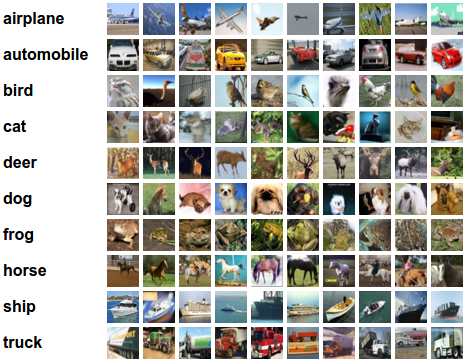
\includegraphics[width=.65\textwidth]{../SOURCE/images/cifar_samples.png}
\caption{}
\end{figure}

想了解更多信息请参考\href{http://www.cs.toronto.edu/~kriz/cifar.html}{CIFAR-10 page},以及Alex Krizhevsky写的\href{http://www.cs.toronto.edu/~kriz/learning-features-2009-TR.pdf}{技术报告}。

\subsubsection {目标}
本教程的目标是建立一个用于识别图像的相对较小的卷积神经网络,在这一过程中,本教程会:

\begin{itemize}
\item 着重于建立一个规范的网络组织结构,训练并进行评估;
\item 为建立更大规模更加复杂的模型提供一个范例
\end{itemize}

选择CIFAR-10是因为它的复杂程度足以用来检验TensorFlow中的大部分功能,并可将其扩展为更大的模型。与此同时由于模型较小所以训练速度很快,比较适合用来测试新的想法,检验新的技术。

\subsubsection {本教程的重点}
CIFAR-10 教程演示了在TensorFlow上构建更大更复杂模型的几个种重要内容:

\begin{itemize}
\item 相关核心数学对象,如卷积、修正线性激活、最大池化以及局部响应归一化;
\item 训练过程中一些网络行为的可视化,这些行为包括输入图像、损失情况、网络行为的分布情况以及梯度;
\item 算法学习参数的移动平均值的计算函数,以及在评估阶段使用这些平均值提高预测性能;
\item 实现了一种机制,使得学习率随着时间的推移而递减;
\item 为输入数据设计预存取队列,将磁盘延迟和高开销的图像预处理操作与模型分离开来处理;
\end{itemize}

我们也提供了模型的多GUP版本,用以表明:

\begin{itemize}
\item 可以配置模型后使其在多个GPU上并行的训练
\item 可以在多个GPU之间共享和更新变量值
\end{itemize}

我们希望本教程给大家开了个头,使得在Tensorflow上可以为视觉相关工作建立更大型的Cnns模型

\subsubsection {模型架构}

本教程中的模型是一个多层架构,由卷积层和非线性层(nonlinearities)交替多次排列后构成。这些层最终通过全连通层对接到softmax分类器上。这一模型除了最顶部的几层外,基本跟Alex Krizhevsky提出的模型一致。

在一个GPU上经过几个小时的训练后,该模型达到了最高86\%的精度。细节请查看下面的描述以及代码。模型中包含了1,068,298个学习参数,分类一副图像需要大概19.5M个乘加操作。

\subsection {Code Organization}

本教程的代码位于\href{https://tensorflow.googlesource.com/tensorflow/+/master/tensorflow/models/image/cifar10/}{tensorflow/models/image/cifar10/}.

% insert table here


\begin{longtable}[c]{@{}ll@{}}
\toprule
\begin{minipage}[b]{0.05\columnwidth}\raggedright\strut
文件
\strut\end{minipage} &
\begin{minipage}[b]{0.05\columnwidth}\raggedright\strut
作用
\strut\end{minipage}\tabularnewline
\midrule
\endhead
\begin{minipage}[t]{0.05\columnwidth}\raggedright\strut
\href{https://tensorflow.googlesource.com/tensorflow/+/master/tensorflow/models/image/cifar10/cifar10_input.py}{\lstinline{cifar10\_input.py}}
\strut\end{minipage} &
\begin{minipage}[t]{0.05\columnwidth}\raggedright\strut
读取本地CIFAR-10的二进制文件格式的内容。
\strut\end{minipage}\tabularnewline
\begin{minipage}[t]{0.05\columnwidth}\raggedright\strut
\href{https://tensorflow.googlesource.com/tensorflow/+/master/tensorflow/models/image/cifar10/cifar10.py}{\lstinline{cifar10.py}}
\strut\end{minipage} &
\begin{minipage}[t]{0.05\columnwidth}\raggedright\strut
建立CIFAR-10的模型。
\strut\end{minipage}\tabularnewline
\begin{minipage}[t]{0.05\columnwidth}\raggedright\strut
\href{https://tensorflow.googlesource.com/tensorflow/+/master/tensorflow/models/image/cifar10/cifar10_train.py}{\lstinline{cifar10\_train.py}}
\strut\end{minipage} &
\begin{minipage}[t]{0.05\columnwidth}\raggedright\strut
在CPU或GPU上训练CIFAR-10的模型。
\strut\end{minipage}\tabularnewline
\begin{minipage}[t]{0.05\columnwidth}\raggedright\strut
\href{https://tensorflow.googlesource.com/tensorflow/+/master/tensorflow/models/image/cifar10/cifar10_multi_gpu_train.py}{\lstinline{cifar10\_multi\_gpu\_train.py}}
\strut\end{minipage} &
\begin{minipage}[t]{0.05\columnwidth}\raggedright\strut
在多GPU上训练CIFAR-10的模型。
\strut\end{minipage}\tabularnewline
\begin{minipage}[t]{0.05\columnwidth}\raggedright\strut
\href{https://tensorflow.googlesource.com/tensorflow/+/master/tensorflow/models/image/cifar10/cifar10_eval.py}{\lstinline{cifar10\_eval.py}}
\strut\end{minipage} &
\begin{minipage}[t]{0.05\columnwidth}\raggedright\strut
评估CIFAR-10模型的预测性能。
\strut\end{minipage}\tabularnewline
\bottomrule
\end{longtable}

\subsection{CIFAR-10 模型 }\label{cifar-10-ux6a21ux578b}

CIFAR-10 网络模型部分的代码位于\href{https://tensorflow.googlesource.com/tensorflow/+/master/tensorflow/models/image/cifar10/cifar10.py}{\lstinline{cifar10.py}}。完整的训练图中包含约765个操作,但是通过下面的模块来构造训练图可以最大限度的提高代码复用率:

\begin{enumerate}
\def\labelenumi{\arabic{enumi}.}
\tightlist
\item
  \protect\hyperlink{model-inputs}{\textbf{模型输入:}}
  包括\lstinline{inputs()} 、
  \lstinline{distorted\_inputs()}等一些操作,分别用于读取CIFAR的图像并进行预处理,做为后续评估和训练的输入;
\item
  \protect\hyperlink{model-prediction}{\textbf{模型预测:}}
  包括\lstinline{inference()}等一些操作,用于进行统计计算,比如在提供的图像进行分类;
  adds operations that perform inference, i.e.~classification, on
  supplied images.
\item
  \protect\hyperlink{model-training}{\textbf{模型训练:}}
  包括\lstinline{loss()} 和
  \lstinline{train()}等一些操作,用于计算损失、计算梯度、进行变量更新以及呈现最终结果。
\end{enumerate}

\subsubsection{模型输入 }\label{ux6a21ux578bux8f93ux5165}

输入模型是通过 \lstinline{inputs()}
和\lstinline{distorted\_inputs()}函数建立起来的,这2个函数会从CIFAR-10二进制文件中读取图片文件,由于每个图片的存储字节数是固定的,因此可以使用\href{https://github.com/jikexueyuanwiki/tensorflow-zh/blob/master/SOURCE/api_docs/python/io_ops.md\#FixedLengthRecordReader}{\lstinline{tf.FixedLengthRecordReader}}函数。更多的关于\lstinline{Reader}类的功能可以查看\href{https://github.com/jikexueyuanwiki/tensorflow-zh/blob/master/SOURCE/how_tos/reading_data/index.md\#reading-from-files}{Reading
Data}。

图片文件的处理流程如下:

\begin{itemize}
\tightlist
\item
  图片会被统一裁剪到24x24像素大小,裁剪中央区域用于评估或\href{https://github.com/jikexueyuanwiki/tensorflow-zh/blob/master/SOURCE/api_docs/python/image.md\#random_crop}{随机}裁剪用于训练;
\item
  图片会进行\href{https://github.com/jikexueyuanwiki/tensorflow-zh/blob/master/SOURCE/api_docs/python/image.md\#per_image_whitening}{近似的白化处理},使得模型对图片的动态范围变化不敏感。
\end{itemize}

对于训练,我们另外采取了一系列随机变换的方法来人为的增加数据集的大小:

\begin{itemize}
\tightlist
\item
  对图像进行\href{https://github.com/jikexueyuanwiki/tensorflow-zh/blob/master/SOURCE/api_docs/python/image.md\#random_flip_left_right}{随机的左右翻转};
\item
  随机变换\href{https://github.com/jikexueyuanwiki/tensorflow-zh/blob/master/SOURCE/api_docs/python/image.md\#random_brightness}{图像的亮度};
\item
  随机变换\href{https://github.com/jikexueyuanwiki/tensorflow-zh/blob/master/SOURCE/api_docs/python/image.md\#tf_image_random_contrast}{图像的对比度};
\end{itemize}

可以在\href{https://github.com/jikexueyuanwiki/tensorflow-zh/blob/master/SOURCE/api_docs/python/image.md}{Images}页的列表中查看所有可用的变换,对于每个原始图我们还附带了一个\href{https://github.com/jikexueyuanwiki/tensorflow-zh/blob/master/SOURCE/api_docs/python/train.md\#image_summary}{\lstinline{image\_summary}},以便于在TensorBoard中查看。这对于检查输入图像是否正确十分有用。

从磁盘上加载图像并进行变换需要花费不少的处理时间。为了避免这些操作减慢训练过程,我们在16个独立的线程中并行进行这些操作,这16个线程被连续的安排在一个TensorFlow\href{https://github.com/jikexueyuanwiki/tensorflow-zh/blob/master/SOURCE/api_docs/python/io_ops.md\#shuffle_batch}{队列}中。

\subsubsection{模型预测 }\label{ux6a21ux578bux9884ux6d4b}

模型的预测流程由\lstinline{inference()}构造,该函数会添加必要的操作步骤用于计算预测值的
\emph{logits},其对应的模型组织方式如下所示:

\begin{longtable}[c]{@{}ll@{}}
\toprule
\begin{minipage}[b]{0.05\columnwidth}\raggedright\strut
Layer 名称
\strut\end{minipage} &
\begin{minipage}[b]{0.05\columnwidth}\raggedright\strut
描述
\strut\end{minipage}\tabularnewline
\midrule
\endhead
\begin{minipage}[t]{0.05\columnwidth}\raggedright\strut
\lstinline{conv1}
\strut\end{minipage} &
\begin{minipage}[t]{0.05\columnwidth}\raggedright\strut
实现\href{https://github.com/jikexueyuanwiki/tensorflow-zh/blob/master/SOURCE/api_docs/python/nn.md\#conv2d}{卷积}
以及
\href{https://github.com/jikexueyuanwiki/tensorflow-zh/blob/master/SOURCE/api_docs/python/nn.md\#relu}{rectified
linear} activation.
\strut\end{minipage}\tabularnewline
\begin{minipage}[t]{0.05\columnwidth}\raggedright\strut
\lstinline{pool1}
\strut\end{minipage} &
\begin{minipage}[t]{0.05\columnwidth}\raggedright\strut
\href{https://github.com/jikexueyuanwiki/tensorflow-zh/blob/master/SOURCE/api_docs/python/nn.md\#max_pool}{max
pooling}.
\strut\end{minipage}\tabularnewline
\begin{minipage}[t]{0.05\columnwidth}\raggedright\strut
\lstinline{norm1}
\strut\end{minipage} &
\begin{minipage}[t]{0.05\columnwidth}\raggedright\strut
\href{https://github.com/jikexueyuanwiki/tensorflow-zh/blob/master/SOURCE/api_docs/python/nn.md\#local_response_normalization}{局部响应归一化}.
\strut\end{minipage}\tabularnewline
\begin{minipage}[t]{0.05\columnwidth}\raggedright\strut
\lstinline{conv2}
\strut\end{minipage} &
\begin{minipage}[t]{0.05\columnwidth}\raggedright\strut
\href{https://github.com/jikexueyuanwiki/tensorflow-zh/blob/master/SOURCE/api_docs/python/nn.md\#conv2d}{卷积}
and
\href{https://github.com/jikexueyuanwiki/tensorflow-zh/blob/master/SOURCE/api_docs/python/nn.md\#relu}{rectified
linear} activation.
\strut\end{minipage}\tabularnewline
\begin{minipage}[t]{0.05\columnwidth}\raggedright\strut
\lstinline{norm2}
\strut\end{minipage} &
\begin{minipage}[t]{0.05\columnwidth}\raggedright\strut
\href{https://github.com/jikexueyuanwiki/tensorflow-zh/blob/master/SOURCE/api_docs/python/nn.md\#local_response_normalization}{局部响应归一化}.
\strut\end{minipage}\tabularnewline
\begin{minipage}[t]{0.05\columnwidth}\raggedright\strut
\lstinline{pool2}
\strut\end{minipage} &
\begin{minipage}[t]{0.05\columnwidth}\raggedright\strut
\href{https://github.com/jikexueyuanwiki/tensorflow-zh/blob/master/SOURCE/api_docs/python/nn.md\#max_pool}{max
pooling}.
\strut\end{minipage}\tabularnewline
\begin{minipage}[t]{0.05\columnwidth}\raggedright\strut
\lstinline{local3}
\strut\end{minipage} &
\begin{minipage}[t]{0.05\columnwidth}\raggedright\strut
\href{https://github.com/jikexueyuanwiki/tensorflow-zh/blob/master/SOURCE/api_docs/python/nn.md}{基于修正线性激活的全连接层}.
\strut\end{minipage}\tabularnewline
\begin{minipage}[t]{0.05\columnwidth}\raggedright\strut
\lstinline{local4}
\strut\end{minipage} &
\begin{minipage}[t]{0.05\columnwidth}\raggedright\strut
\href{https://github.com/jikexueyuanwiki/tensorflow-zh/blob/master/SOURCE/api_docs/python/nn.md}{基于修正线性激活的全连接层}.
\strut\end{minipage}\tabularnewline
\begin{minipage}[t]{0.05\columnwidth}\raggedright\strut
\lstinline{softmax\_linear}
\strut\end{minipage} &
\begin{minipage}[t]{0.05\columnwidth}\raggedright\strut
进行线性变换以输出 logits.
\strut\end{minipage}\tabularnewline
\bottomrule
\end{longtable}

这里有一个由TensorBoard绘制的图形,用于描述模型建立过程中经过的步骤:

\begin{quote}
\textbf{练习}:
\lstinline{inference}的输出是未归一化的logits,尝试使用\href{tensorflow-zh/SOURCE/api_docs/python/nn.md\#softmax}{\lstinline{tf.softmax()}}修改网络架构后返回归一化的预测值。
\end{quote}

\lstinline{inputs()} 和 \lstinline{inference()}
函数提供了评估模型时所需的所有构件,现在我们把讲解的重点从构建一个模型转向训练一个模型。

\begin{quote}
\textbf{练习:} \lstinline{inference()}
中的模型跟\href{https://code.google.com/p/cuda-convnet/}{cuda-convnet}中描述的CIFAR-10模型有些许不同,其差异主要在于其顶层不是全连接层而是局部连接层,可以尝试修改网络架构来准确的复制全连接模型。
\end{quote}

\subsubsection{模型训练}\label{ux6a21ux578bux8badux7ec3}

训练一个可进行N维分类的网络的常用方法是使用\href{https://en.wikipedia.org/wiki/Multinomial_logistic_regression}{多项式逻辑回归},又被叫做\emph{softmax
回归}。Softmax
回归在网络的输出层上附加了一个\href{https://github.com/jikexueyuanwiki/tensorflow-zh/blob/master/SOURCE/api_docs/python/nn.md\#softmax}{softmax}
nonlinearity,并且计算归一化的预测值和label的\href{https://github.com/jikexueyuanwiki/tensorflow-zh/blob/master/SOURCE/api_docs/python/sparse_ops.md\#sparse_to_dense}{1-hot
encoding}的\href{https://github.com/jikexueyuanwiki/tensorflow-zh/blob/master/SOURCE/api_docs/python/nn.md\#softmax_cross_entropy_with_logits}{交叉熵}。在正则化过程中,我们会对所有学习变量应用\href{https://github.com/jikexueyuanwiki/tensorflow-zh/blob/master/SOURCE/api_docs/python/nn.md\#l2_loss}{权重衰减损失}。模型的目标函数是求交叉熵损失和所有权重衰减项的和,\lstinline{loss()}函数的返回值就是这个值。

在TensorBoard中使用\href{https://github.com/jikexueyuanwiki/tensorflow-zh/blob/master/SOURCE/api_docs/python/train.md\#scalar_summary}{scalar\_summary}来查看该值的变化情况:

\begin{figure}[htbp]
\centering
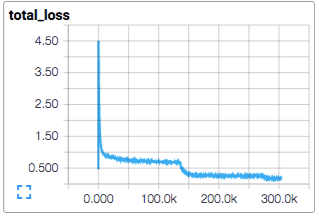
\includegraphics{../SOURCE/images/cifar_loss.png}
\caption{CIFAR-10 Loss}
\end{figure}

我们使用标准的梯度下降算法来训练模型(也可以在\href{https://github.com/jikexueyuanwiki/tensorflow-zh/blob/master/SOURCE/api_docs/python/train.md}{Training}中看看其他方法),其学习率随时间以指数形式衰减。

\begin{figure}[htbp]
\centering
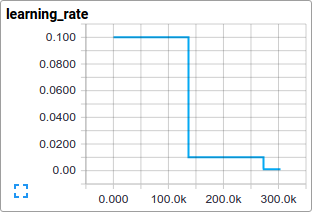
\includegraphics{../SOURCE/images/cifar_lr_decay.png}
\caption{CIFAR-10 Learning Rate Decay}
\end{figure}

\lstinline{train()}
函数会添加一些操作使得目标函数最小化,这些操作包括计算梯度、更新学习变量(详细信息请查看\href{tensorflow-zh/SOURCE/api_docs/python/train.md\#GradientDescentOptimizer}{\lstinline{GradientDescentOptimizer}})。\lstinline{train()}
函数最终会返回一个用以对一批图像执行所有计算的操作步骤,以便训练并更新模型。

\subsection{开始执行并训练模型
}\label{ux5f00ux59cbux6267ux884cux5e76ux8badux7ec3ux6a21ux578b}

我们已经把模型建立好了,现在通过执行脚本\lstinline{cifar10\_train.py}来启动训练过程。

\begin{lstlisting}
python cifar10_train.py
\end{lstlisting}

\textbf{注意:}
当第一次在CIFAR-10教程上启动任何任务时,会自动下载CIFAR-10数据集,该数据集大约有160M大小,因此第一次运行时泡杯咖啡小栖一会吧。

你应该可以看到如下类似的输出:

\begin{lstlisting}
Filling queue with 20000 CIFAR images before starting to train. This will take a few minutes.
2015-11-04 11:45:45.927302: step 0, loss = 4.68 (2.0 examples/sec; 64.221 sec/batch)
2015-11-04 11:45:49.133065: step 10, loss = 4.66 (533.8 examples/sec; 0.240 sec/batch)
2015-11-04 11:45:51.397710: step 20, loss = 4.64 (597.4 examples/sec; 0.214 sec/batch)
2015-11-04 11:45:54.446850: step 30, loss = 4.62 (391.0 examples/sec; 0.327 sec/batch)
2015-11-04 11:45:57.152676: step 40, loss = 4.61 (430.2 examples/sec; 0.298 sec/batch)
2015-11-04 11:46:00.437717: step 50, loss = 4.59 (406.4 examples/sec; 0.315 sec/batch)
...
\end{lstlisting}

脚本会在每10步训练过程后打印出总损失值,以及最后一批数据的处理速度。下面是几点注释:

\begin{itemize}
\item
  第一批数据会非常的慢(大概要几分钟时间),因为预处理线程要把20,000个待处理的CIFAR图像填充到重排队列中;
\item
  打印出来的损失值是最近一批数据的损失值的均值。请记住损失值是交叉熵和权重衰减项的和;
\item
  上面打印结果中关于一批数据的处理速度是在Tesla
  K40C上统计出来的,如果你运行在CPU上,性能会比此要低;
\end{itemize}

\begin{quote}
\textbf{练习:}
当实验时,第一阶段的训练时间有时会非常的长,长到足以让人生厌。可以尝试减少初始化时初始填充到队列中图片数量来改变这种情况。在\lstinline{cifar10.py}中搜索\lstinline{NUM\_EXAMPLES\_PER\_EPOCH\_FOR\_TRAIN}并修改之。
\end{quote}

\lstinline{cifar10\_train.py}
会周期性的在\href{https://github.com/jikexueyuanwiki/tensorflow-zh/tree/master/SOURCE/how_tos/variables/index.md\#saving-and-restoring}{检查点文件}中\href{https://github.com/jikexueyuanwiki/tensorflow-zh/blob/master/SOURCE/api_docs/python/state_ops.md\#Saver}{保存}模型中的所有参数,但是\emph{不会}对模型进行评估。\lstinline{cifar10\_eval.py}会使用该检查点文件来测试预测性能(详见下面的描述:\protect\hyperlink{ux8bc4ux4f30ux6a21ux578b}{评估模型})。

如果按照上面的步骤做下来,你应该已经开始训练一个CIFAR-10模型了。\href{https://www.youtube.com/watch?v=9bZkp7q19f0}{恭喜你!}

\lstinline{cifar10\_train.py}输出的终端信息中提供了关于模型如何训练的一些信息,但是我们可能希望了解更多关于模型训练时的信息,比如:\\
* 损失是\emph{真的}在减小还是看到的只是噪声数据?\\
* 为模型提供的图片是否合适?\\
* 梯度、激活、权重的值是否合理?\\
* 当前的学习率是多少?

\href{https://github.com/jikexueyuanwiki/tensorflow-zh/tree/master/SOURCE/how_tos/summaries_and_tensorboard/index.md}{TensorBoard}提供了该功能,可以通过\lstinline{cifar10\_train.py}中的\href{https://github.com/jikexueyuanwiki/tensorflow-zh/blob/master/SOURCE/api_docs/python/train.md\#SummaryWriter}{\lstinline{SummaryWriter}}周期性的获取并显示这些数据。

比如我们可以在训练过程中查看\lstinline{local3}的激活情况,以及其特征维度的稀疏情况:

相比于总损失,在训练过程中的单项损失尤其值得人们的注意。但是由于训练中使用的数据批量比较小,损失值中夹杂了相当多的噪声。在实践过程中,我们也发现相比于原始值,损失值的移动平均值显得更为有意义。请参阅脚本\href{https://github.com/jikexueyuanwiki/tensorflow-zh/blob/master/SOURCE/api_docs/python/train.md\#ExponentialMovingAverage}{\lstinline{ExponentialMovingAverage}}了解如何实现。

\hypertarget{ux8bc4ux4f30ux6a21ux578b}{\subsection{评估模型
}\label{ux8bc4ux4f30ux6a21ux578b}}

现在可以在另一部分数据集上来评估训练模型的性能。脚本文件\lstinline{cifar10\_eval.py}对模型进行了评估,利用
\lstinline{inference()}函数重构模型,并使用了在评估数据集所有10,000张CIFAR-10图片进行测试。最终计算出的精度为\emph{1:N},N=预测值中置信度最高的一项与图片真实label匹配的频次。(It
calculates the \emph{precision at 1:} how often the top prediction
matches the true label of the image)。

为了监控模型在训练过程中的改进情况,评估用的脚本文件会周期性的在最新的检查点文件上运行,这些检查点文件是由\lstinline{cifar10\_train.py}产生。

\begin{lstlisting}
python cifar10_eval.py
\end{lstlisting}

\begin{quote}
注意:不要在同一块GPU上同时运行训练程序和评估程序,因为可能会导致内存耗尽。尽可能的在其它单独的GPU上运行评估程序,或者在同一块GPU上运行评估程序时先挂起训练程序。
\end{quote}

你可能会看到如下所示输出:

\begin{lstlisting}
2015-11-06 08:30:44.391206: precision @ 1 = 0.860
...
\end{lstlisting}

评估脚本只是周期性的返回precision@1 (The script merely returns the
precision @ 1
periodically)--在该例中返回的准确率是86\%。\lstinline{cifar10\_eval.py}
同时也返回其它一些可以在TensorBoard中进行可视化的简要信息。可以通过这些简要信息在评估过程中进一步的了解模型。

训练脚本会为所有学习变量计算其\href{https://github.com/jikexueyuanwiki/tensorflow-zh/blob/master/SOURCE/api_docs/python/train.md\#ExponentialMovingAverage}{移动均值},评估脚本则直接将所有学习到的模型参数替换成对应的移动均值。这一替代方式可以在评估过程中提升模型的性能。

\begin{quote}
\textbf{练习:} 通过precision @
1测试发现,使用均值参数可以将预测性能提高约3\%,在\lstinline{cifar10\_eval.py}中尝试修改为不采用均值参数的方式,并确认由此带来的预测性能下降。
\end{quote}

\subsection{在多个GPU板卡上训练模型
}\label{ux5728ux591aux4e2agpuux677fux5361ux4e0aux8badux7ec3ux6a21ux578b}

现代的工作站可能包含多个GPU进行科学计算。TensorFlow可以利用这一环境在多个GPU卡上运行训练程序。

在并行、分布式的环境中进行训练,需要对训练程序进行协调。对于接下来的描述,术语\emph{模型拷贝}(\emph{model
replica})特指在一个数据子集中训练出来的模型的一份拷贝。

如果天真的对模型参数的采用异步方式更新将会导致次优的训练性能,这是因为我们可能会基于一个旧的模型参数的拷贝去训练一个模型。但与此相反采用完全同步更新的方式,其速度将会变得和最慢的模型一样慢(Conversely,
employing fully synchronous updates will be as slow as the slowest model
replica.)。

在具有多个GPU的工作站中,每个GPU的速度基本接近,并且都含有足够的内存来运行整个CIFAR-10模型。因此我们选择以下方式来设计我们的训练系统:

\begin{itemize}
\item
  在每个GPU上放置单独的模型副本;
\item
  等所有GPU处理完一批数据后再同步更新模型的参数;
\end{itemize}

下图示意了该模型的结构::

可以看到,每一个GPU会用一批独立的数据计算梯度和估计值。这种设置可以非常有效的将一大批数据分割到各个GPU上。

这一机制要求所有GPU能够共享模型参数。但是众所周知在GPU之间传输数据非常的慢,因此我们决定在CPU上存储和更新所有模型的参数(对应图中绿色矩形的位置)。这样一来,GPU在处理一批新的数据之前会更新一遍的参数。

图中所有的GPU是同步运行的。所有GPU中的梯度会累积并求平均值(绿色方框部分)。模型参数会利用所有模型副本梯度的均值来更新。

\subsubsection{在多个设备中设置变量和操作}\label{ux5728ux591aux4e2aux8bbeux5907ux4e2dux8bbeux7f6eux53d8ux91cfux548cux64cdux4f5c}

在多个设备中设置变量和操作时需要做一些特殊的抽象。

我们首先需要把在单个模型拷贝中计算估计值和梯度的行为抽象到一个函数中。在代码中,我们称这个抽象对象为``tower''。对于每一个``tower''我们都需要设置它的两个属性:\\
*
在一个tower中为所有操作设定一个唯一的名称。\href{https://github.com/jikexueyuanwiki/tensorflow-zh/blob/master/SOURCE/api_docs/python/framework.md\#name_scope}{\lstinline{tf.name\_scope()}}通过添加一个范围前缀来提供该唯一名称。比如,第一个tower中的所有操作都会附带一个前缀\lstinline{tower\_0},示例:\lstinline{tower\_0/conv1/Conv2D};

\begin{itemize}
\tightlist
\item
  在一个tower中运行操作的优先硬件设备。
  \href{https://github.com/jikexueyuanwiki/tensorflow-zh/blob/master/SOURCE/api_docs/python/framework.md\#device}{\lstinline{tf.device()}}
  提供该信息。比如,在第一个tower中的所有操作都位于
  \lstinline{device(\textquotesingle{}/gpu:0\textquotesingle{})}范围中,暗含的意思是这些操作应该运行在第一块GPU上;
\end{itemize}

为了在多个GPU上共享变量,所有的变量都绑定在CPU上,并通过\href{https://github.com/jikexueyuanwiki/tensorflow-zh/blob/master/SOURCE/api_docs/python/state_ops.md\#get_variable}{\lstinline{tf.get\_variable()}}访问。可以查看\href{https://github.com/jikexueyuanwiki/tensorflow-zh/blob/master/SOURCE/how_tos/variables/index.md}{Sharing
Variables}以了解如何共享变量。

\subsubsection{启动并在多个GPU上训练模型
}\label{ux542fux52a8ux5e76ux5728ux591aux4e2agpuux4e0aux8badux7ec3ux6a21ux578b}

如果你的机器上安装有多块GPU,你可以通过使用\lstinline{cifar10\_multi\_gpu\_train.py}脚本来加速模型训练。该脚本是训练脚本的一个变种,使用多个GPU实现模型并行训练。

\begin{lstlisting}
python cifar10_multi_gpu_train.py --num_gpus=2
\end{lstlisting}

训练脚本的输出如下所示:

\begin{lstlisting}
Filling queue with 20000 CIFAR images before starting to train. This will take a few minutes.
2015-11-04 11:45:45.927302: step 0, loss = 4.68 (2.0 examples/sec; 64.221 sec/batch)
2015-11-04 11:45:49.133065: step 10, loss = 4.66 (533.8 examples/sec; 0.240 sec/batch)
2015-11-04 11:45:51.397710: step 20, loss = 4.64 (597.4 examples/sec; 0.214 sec/batch)
2015-11-04 11:45:54.446850: step 30, loss = 4.62 (391.0 examples/sec; 0.327 sec/batch)
2015-11-04 11:45:57.152676: step 40, loss = 4.61 (430.2 examples/sec; 0.298 sec/batch)
2015-11-04 11:46:00.437717: step 50, loss = 4.59 (406.4 examples/sec; 0.315 sec/batch)
...
\end{lstlisting}

需要注意的是默认的GPU使用数是1,此外,如果你的机器上只有一个GPU,那么所有的计算都只会在一个GPU上运行,即便你可能设置的是N个。

\begin{quote}
\textbf{练习:}
\lstinline{cifar10\_train.py}中的批处理大小默认配置是128。尝试在2个GPU上运行\lstinline{cifar10\_multi\_gpu\_train.py}脚本,并且设定批处理大小为64,然后比较2种方式的训练速度。
\end{quote}

\subsection{下一步 }\label{ux4e0bux4e00ux6b65}

恭喜你! 你已经完成了CIFAR-10教程。 如果你对开发和训练自己的图像分类系统感兴趣,我们推荐你新建一个基于该教程的分支,并修改其中的内容以建立解决您问题的图像分类系统。

\begin{quote}
\textbf{练习:} 下载\href{http://ufldl.stanford.edu/housenumbers/}{Street
View House Numbers (SVHN)}
数据集。新建一个CIFAR-10教程的分支,并将输入数据替换成SVHN。尝试改变网络结构以提高预测性能。
\end{quote}

\begin{quote}
原文:\href{http://tensorflow.org/tutorials/deep_cnn/index.md}{Convolutional
Neural Networks} 翻译:\href{https://github.com/oskycar}{oskycar}
校对:\href{https://github.com/zhyhooo}{KK4SBB}
\end{quote}

%!TEX program = xelatex
% Encoding: UTF8
% SEIKA 2015

\section{Vector Representations of Words}\label{word2vec}

In this tutorial we look at the word2vec model by \href{http://papers.nips.cc/paper/5021-distributed-representations-of-words-and-phrases-and-their-compositionality.pdf}{Mikolov et al}. This model is used for learning vector representations of words, called "word embeddings".

在本教程我们来看一下\href{http://papers.nips.cc/paper/5021-distributed-representations-of-words-and-phrases-and-their-compositionality.pdf}{Mikolovet al}中提到的word2vec模型。该模型是用于学习文字的向量表示,称之为 "wordembedding"。

\subsection{亮点 }\label{word2vec_hl}

本教程旨在意在展现出在TensorfLow中构建word2vec模型有趣、本质的部分。

\begin{itemize}
\item 我们从我们为何需要使用向量表示文字开始。
\item 我们通过直观地例子观察模型背后的本质,以及它是如何训练的(通过一些数学方法评估)。
\item 同时我们也展示了TensorFlow对该模型的简单实现。
\item 最后,我们着眼于让给这个简单版本的模型表现更好。
\end{itemize}

我们会在教程的推进中循序渐进地解释代码,但是如果你更希望直入主题,可以在
\href{https://tensorflow.googlesource.com/tensorflow/+/master/tensorflow/g3doc/tutorials/word2vec/word2vec_basic.py}{tensorflow/g3doc/tutorials/word2vec/word2vec\_basic.py}查看到一个最简单的实现。这个基本的例子提供的代码可以完成下载一些数据,简单训练后展示结果。一旦你觉得已经完全掌握了这个简单版本,你可以查看
\href{https://tensorflow.googlesource.com/tensorflow/+/master/tensorflow/models/embedding/word2vec.py}{tensorflow/models/embedding/word2vec.py},这里提供了一些更复杂的实现,同时也展示了TensorFlow的一些更进阶的特性,比如如何更高效地使用线程将数据送入文本模型,再比如如何在训练中设置检查点等等。

但是首先,让我们来看一下为何需要学习word embeddings。如果你对word
embeddings相关内容已经是个专家了,那么请安心跳过本节内容,直接深入细节干一些脏活吧。

\subsection{动机: 为什么需要学习 Word Embeddings?}\label{ux52a8}

通常图像或音频系统处理的是由图片中所有单个原始像素点强度值或者音频中功率谱密度的强度值,把它们编码成丰富、高纬度的向量数据集。对于物体或语音识别这一类的任务,我们所需的全部信息已经都存储在原始数据中(显然人类本身就是依赖原始数据进行日常的物体或语音识别的)。然后,自然语言处理系统通常将词汇作为离散的单一符号,例如"cat" 一词或可表示为\lstinline{Id537} ,而"dog"一词或可表示为\lstinline{Id143}。这些符号编码毫无规律,无法提供不同词汇之间可能存在的关联信息。换句话说,在处理关于"dogs" 一词的信息时,模型将无法利用已知的关于"cats"的信息(例如,它们都是动物,有四条腿,可作为宠物等等)。可见,将词汇表达为上述的独立离散符号将进一步导致数据稀疏,使我们在训练统计模型时不得不寻求更多的数据。而词汇的向量表示将克服上述的难题。

\href{https://en.wikipedia.org/wiki/Vector_space_model}{向量空间模型(VSMs)}
将词汇表达(嵌套)于一个连续的向量空间中,语义近似的词汇被映射为相邻的数据点。向量空间模型在自然语言处理领域中有着漫长且丰富的历史,不过几乎所有利用这一模型的方法都依赖于\href{https://en.wikipedia.org/wiki/Distributional_semantics\#Distributional_Hypothesis}{分布式假设},其核心思想为出现于上下文情景中的词汇都有相类似的语义。采用这一假设的研究方法大致分为以下两类:\emph{基于技术的方法}(如,\href{https://en.wikipedia.org/wiki/Latent_semantic_analysis}{潜在语义分析}),和 \emph{预测方法} (如,\href{http://www.scholarpedia.org/article/Neural_net_language_models}{神经概率化语言模型}).

其中它们的区别在如下论文中又详细阐述\href{http://clic.cimec.unitn.it/marco/publications/acl2014/baroni-etal-countpredict-acl2014.pdf}{Baroni
etal.},不过简而言之:基于计数的方法计算某词汇与其邻近词汇在一个大型语料库中共同出现的频率及其他统计量,然后将这些统计量映射到一个小型且稠密的向量中。预测方法则试图直接从某词汇的邻近词汇对其进行预测,在此过程中利用已经学习到的小型且稠密的\emph{嵌套向量}。

Word2vec是一种可以进行高效率词嵌套学习的预测模型。其两种变体分别为:连续词袋模型(CBOW)及Skip-Gram模型。从算法角度看,这两种方法非常相似,其区别为CBOW根据源词上下文词汇("the cat sits on the")来预测目标词汇(例如,"mat"),而Skip-Gram模型做法相反,它通过目标词汇来预测源词汇。Skip-Gram模型采取CBOW的逆过程的动机在于:CBOW算法对于很多分布式信息进行了平滑处理(例如将一整段上下文信息视为一个单一观察量)。很多情况下,对于小型的数据集,这一处理是有帮助的。相形之下,Skip-Gram模型将每个“上下文---目标词汇”的组合视为一个新观察量,这种做法在大型数据集中会更为有效。本教程余下部分将着重讲解Skip-Gram模型。

\subsection{处理噪声对比训练}\label{ux5904ux7406ux566aux58f0ux5bf9ux6bd4ux8badux7ec3}

神经概率化语言模型通常使用\href{https://en.wikipedia.org/wiki/Maximum_likelihood}{极大似然法(ML)} 进行训练,其中通过\href{https://en.wikipedia.org/wiki/Softmax_function}{\emph{softmax}function} 来最大化当提供前一个单词$h$ (代表"history"),后一个单词的概率$w_t$ (代表"target"),

\begin{figure}[htbp]
\centering
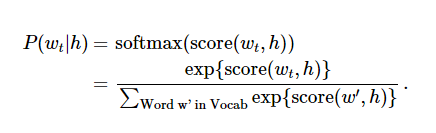
\includegraphics{../SOURCE/images/vr2.png}
\caption{}
\end{figure}

当$score(w_t,h)$ 计算了文字 $w_t$ 和 上下文 $h$的相容性(通常使用向量积)。我们使用对数似然函数来训练训练集的最大值,比如通过:

\begin{align}
P(w_t|h) & = softmax(score(w_t,h)) \\
         & = \frac{exp\{score(w_t,h)\}}{\sum_{Word w'in Vocab}{exp\{score(w',h)\}}}
\end{align}

\begin{figure}[htbp]
\centering
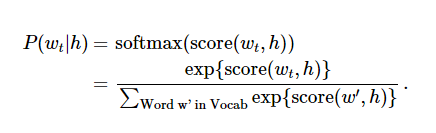
\includegraphics{../SOURCE/images/vr2.png}
\caption{}
\end{figure}

这里提出了一个解决语言概率模型的合适的通用方法。然而这个方法实际执行起来开销非常大,因为我们需要去计算并正则化当前上下文环境
\textbf{h} 中所有其他 \textbf{V} 单词 \textbf{w'}
的概率得分,\emph{在每一步训练迭代中}。

从另一个角度来说,当使用word2vec模型时,我们并不需要对概率模型中的所有特征进行学习。而CBOW模型和Skip-Gram模型为了避免这种情况发生,使用一个二分类器(逻辑回归)在同一个上下文环境里从
\textbf{k} 虚构的 (噪声) 单词 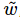
\includegraphics{../SOURCE/images/rw5.png}
区分出真正的目标单词
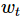
\includegraphics{../SOURCE/images/rw4.png}。我们下面详细阐述一下CBOW模型,对于Skip-Gram模型只要简单地做相反的操作即可。

从数学角度来说,我们的目标是对每个样本最大化:

\begin{figure}[htbp]
\centering
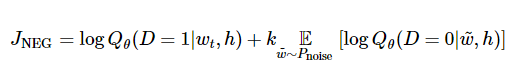
\includegraphics{../SOURCE/images/rw6.png}
\caption{}
\end{figure}

其中 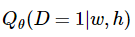
\includegraphics{../SOURCE/images/rw7.png} 代表的是数据集在当前上下文\textbf{h} ,根据所学习的嵌套向量 
\includegraphics{../SOURCE/images/theta.png},目标单词 \textbf{w}使用二分类逻辑回归计算得出的概率。在实践中,我们通过在噪声分布中绘制比对文字来获得近似的期望值(通过计算\href{https://en.wikipedia.org/wiki/Monte_Carlo_integration}{蒙特卡洛平均值})。

当真实地目标单词被分配到较高的概率,同时噪声单词的概率很低时,目标函数也就达到最大值了。从技术层面来说,这种方法叫做\href{http://papers.nips.cc/paper/5021-distributed-representations-of-words-and-phrases-and-their-compositionality.pdf}{负抽样},而且使用这个损失函数在数学层面上也有很好的解释:这个更新过程也近似于softmax函数的更新。这在计算上将会有很大的优势,因为当计算这个损失函数时,只是有我们挑选出来的\textbf{k} 个 \emph{噪声单词},而没有使用整个语料库\textbf{V}。这使得训练变得非常快。我们实际上使用了与\href{http://papers.nips.cc/paper/5165-learning-word-embeddings-efficiently-with-noise-contrastive-estimation.pdf}{noise-contrastiveestimation(NCE)}介绍的非常相似的方法,这在TensorFlow中已经封装了一个很便捷的函数\lstinline{tf.nn.nce_loss()}。

让我们在实践中来直观地体会它是如何运作的!

\subsection{Skip-gram 模型}\label{skip-gram_model}

下面来看一下这个数据集

\lstinline{"the quick brown fox jumped over the lazy dog"}

我们首先对一些单词以及它们的上下文环境建立一个数据集。我们可以以任何合理的方式定义`上下文',而通常上这个方式是根据文字的句法语境的(使用语法原理的方式处理当前目标单词可以看一下这篇文献
\href{https://levyomer.files.wordpress.com/2014/04/dependency-based-word-embeddings-acl-2014.pdf}{Levy et al.},比如说把目标单词左边的内容当做一个“上下文”,或者以目标单词右边的内容,等等。现在我们把目标单词的左右单词视作一个上下文,
使用大小为1的窗口,这样就得到这样一个由\texttt{(上下文,\ 目标单词)}
组成的数据集:

\texttt{({[}the,\ brown{]},\ quick),\ ({[}quick,\ fox{]},\ brown),\ ({[}brown,\ jumped{]},\ fox),\ ...}

前文提到Skip-Gram模型是把目标单词和上下文颠倒过来,所以在这个问题中,举个例子,就是用'quick'来预测
`the' 和 `brown' ,用 `brown' 预测 `quick' 和 `brown'
。因此这个数据集就变成由\texttt{(输入,\ 输出)}组成的:

\texttt{(quick,\ the),\ (quick,\ brown),\ (brown,\ quick),\ (brown,\ fox),\ ...}

目标函数通常是对整个数据集建立的,但是本问题中要对每一个样本(或者是一个\texttt{batch\_size}
很小的样本集,通常设置为\texttt{16\ \textless{}=\ batch\_size\ \textless{}=\ 512})在同一时间执行特别的操作,称之为\href{https://en.wikipedia.org/wiki/Stochastic_gradient_descent}{随机梯度下降}
(SGD)。我们来看一下训练过程中每一步的执行。

假设用 \textbf{t} 表示上面这个例子中\texttt{quick} 来预测 \texttt{the}
的训练的单个循环。用 \texttt{num\_noise}
定义从噪声分布中挑选出来的噪声(相反的)单词的个数,通常使用一元分布,\textbf{P(w)}。为了简单起见,我们就定\texttt{num\_noise=1},用
\texttt{sheep}
选作噪声词。接下来就可以计算每一对观察值和噪声值的损失函数了,每一个执行步骤就可表示为:

\begin{figure}[htbp]
\centering
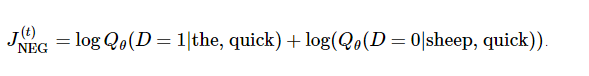
\includegraphics{../SOURCE/images/vr4.png}
\caption{}
\end{figure}

整个计算过程的目标是通过更新嵌套参数

\includegraphics{../SOURCE/images/theta.png}
来逼近目标函数(这个这个例子中就是使目标函数最大化)。为此我们要计算损失函数中嵌套参数

\includegraphics{../SOURCE/images/theta.png} 的梯度,比如,
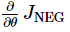
\includegraphics{../SOURCE/images/vr5.png}
(幸好TensorFlow封装了工具函数可以简单调用!)。对于整个数据集,当梯度下降的过程中不断地更新参数,对应产生的效果就是不断地移动每个单词的嵌套向量,直到可以把真实单词和噪声单词很好得区分开。

我们可以把学习向量映射到2维中以便我们观察,其中用到的技术可以参考
\href{http://lvdmaaten.github.io/tsne/}{t-SNE
降纬技术}。当我们用可视化的方式来观察这些向量,就可以很明显的获取单词之间语义信息的关系,这实际上是非常有用的。当我们第一次发现这样的诱导向量空间中,展示了一些特定的语义关系,这是非常有趣的,比如文字中
\emph{male-female},\emph{gender} 甚至还有 \emph{country-capital}
的关系, 如下方的图所示 (也可以参考
\href{http://www.aclweb.org/anthology/N13-1090}{Mikolov et al.,
2013}论文中的例子)。

这也解释了为什么这些向量在传统的NLP问题中可作为特性使用,比如用在对一个演讲章节打个标签,或者对一个专有名词的识别
(看看如下这个例子 \href{http://arxiv.org/pdf/1103.0398v1.pdf}{Collobert
et al.}或者 \href{http://www.aclweb.org/anthology/P10-1040}{Turian et
al.})。

不过现在让我们用它们来画漂亮的图表吧!

\subsection{建立图形 }\label{ux5efaux7acbux56feux5f62}

这里谈得都是嵌套,那么先来定义一个嵌套参数矩阵。我们用唯一的随机值来初始化这个大矩阵。

\begin{Shaded}
\begin{Highlighting}[]
\NormalTok{embeddings }\OperatorTok{=} \NormalTok{tf.Variable(}
    \NormalTok{tf.random_uniform([vocabulary_size, embedding_size], }\OperatorTok{-}\FloatTok{1.0}\NormalTok{, }\FloatTok{1.0}\NormalTok{))}
\end{Highlighting}
\end{Shaded}

对噪声-比对的损失计算就使用一个逻辑回归模型。对此,我们需要对语料库中的每个单词定义一个权重值和偏差值。(也可称之为\texttt{输出权重}
与之对应的 \texttt{输入嵌套值})。定义如下。

\begin{Shaded}
\begin{Highlighting}[]
\NormalTok{nce_weights }\OperatorTok{=} \NormalTok{tf.Variable(}
  \NormalTok{tf.truncated_normal([vocabulary_size, embedding_size],}
                      \NormalTok{stddev}\OperatorTok{=}\FloatTok{1.0} \OperatorTok{/} \NormalTok{math.sqrt(embedding_size)))}
\NormalTok{nce_biases }\OperatorTok{=} \NormalTok{tf.Variable(tf.zeros([vocabulary_size]))}
\end{Highlighting}
\end{Shaded}

我们有了这些参数之后,就可以定义Skip-Gram模型了。简单起见,假设我们已经把语料库中的文字整型化了,这样每个整型代表一个单词(细节请查看
\href{https://tensorflow.googlesource.com/tensorflow/+/master/tensorflow/g3doc/tutorials/word2vec/word2vec_basic.py}{tensorflow/g3doc/tutorials/word2vec/word2vec\_basic.py})。Skip-Gram模型有两个输入。一个是一组用整型表示的上下文单词,另一个是目标单词。给这些输入建立占位符节点,之后就可以填入数据了。

\begin{Shaded}
\begin{Highlighting}[]
\CommentTok{# 建立输入占位符}
\NormalTok{train_inputs }\OperatorTok{=} \NormalTok{tf.placeholder(tf.int32, shape}\OperatorTok{=}\NormalTok{[batch_size])}
\NormalTok{train_labels }\OperatorTok{=} \NormalTok{tf.placeholder(tf.int32, shape}\OperatorTok{=}\NormalTok{[batch_size, }\DecValTok{1}\NormalTok{])}
\end{Highlighting}
\end{Shaded}

然后我们需要对批数据中的单词建立嵌套向量,TensorFlow提供了方便的工具函数。

\begin{Shaded}
\begin{Highlighting}[]
\NormalTok{embed }\OperatorTok{=} \NormalTok{tf.nn.embedding_lookup(embeddings, train_inputs)}
\end{Highlighting}
\end{Shaded}

好了,现在我们有了每个单词的嵌套向量,接下来就是使用噪声-比对的训练方式来预测目标单词。

\begin{Shaded}
\begin{Highlighting}[]
\CommentTok{# 计算 NCE 损失函数, 每次使用负标签的样本.}
\NormalTok{loss }\OperatorTok{=} \NormalTok{tf.reduce_mean(}
  \NormalTok{tf.nn.nce_loss(nce_weights, nce_biases, embed, train_labels,}
                 \NormalTok{num_sampled, vocabulary_size))}
\end{Highlighting}
\end{Shaded}

我们对损失函数建立了图形节点,然后我们需要计算相应梯度和更新参数的节点,比如说在这里我们会使用随机梯度下降法,TensorFlow也已经封装好了该过程。

\begin{Shaded}
\begin{Highlighting}[]
\CommentTok{# 使用 SGD 控制器.}
\NormalTok{optimizer }\OperatorTok{=} \NormalTok{tf.train.GradientDescentOptimizer(learning_rate}\OperatorTok{=}\FloatTok{1.0}\NormalTok{).minimize(loss)}
\end{Highlighting}
\end{Shaded}

\subsection{训练模型 }\label{ux8badux7ec3ux6a21ux578b}

训练的过程很简单,只要在循环中使用\texttt{feed\_dict}不断给占位符填充数据,同时调用
\href{tensorflow-zh/SOURCE/api_docs/python/client.md\#Session.run}{\texttt{session.run}}即可。

\begin{Shaded}
\begin{Highlighting}[]
\ControlFlowTok{for} \NormalTok{inputs, labels }\OperatorTok{in} \NormalTok{generate_batch(...):}
  \NormalTok{feed_dict }\OperatorTok{=} \NormalTok{\{training_inputs: inputs, training_labels: labels\}}
  \NormalTok{_, cur_loss }\OperatorTok{=} \NormalTok{session.run([optimizer, loss], feed_dict}\OperatorTok{=}\NormalTok{feed_dict)}
\end{Highlighting}
\end{Shaded}

完整地例子可参考
\href{./word2vec_basic.py}{tensorflow/g3doc/tutorials/word2vec/word2vec\_basic.py}.

\subsection{嵌套学习结果可视化
}\label{ux5d4cux5957ux5b66ux4e60ux7ed3ux679cux53efux89c6ux5316}

使用t-SNE来看一下嵌套学习完成的结果。

Et voila!
与预期的一样,相似的单词被聚类在一起。对word2vec模型更复杂的实现需要用到TensorFlow一些更高级的特性,具体是实现可以参考
\href{https://tensorflow.googlesource.com/tensorflow/+/master/tensorflow/models/embedding/word2vec.py}{tensorflow/models/embedding/word2vec.py}。

\subsection{嵌套学习的评估: 类比推理
}\label{ux5d4cux5957ux5b66ux4e60ux7684ux8bc4ux4f30-ux7c7bux6bd4ux63a8ux7406}

词嵌套在NLP的预测问题中是非常有用且使用广泛地。如果要检测一个模型是否是可以成熟地区分词性或者区分专有名词的模型,最简单的办法就是直接检验它的预测词性、语义关系的能力,比如让它解决形如\texttt{king\ is\ to\ queen\ as\ father\ is\ to\ ?}这样的问题。这种方法叫做\emph{类比推理}
,可参考\href{http://msr-waypoint.com/en-us/um/people/gzweig/Pubs/NAACL2013Regularities.pdf}{Mikolov
and colleagues},数据集下载地址为:
https://word2vec.googlecode.com/svn/trunk/questions-words.txt。

To see how we do this
evaluation如何执行这样的评估,可以看\texttt{build\_eval\_graph()}和
\texttt{eval()}这两个函数在下面源码中的使用
\href{https://tensorflow.googlesource.com/tensorflow/+/master/tensorflow/models/embedding/word2vec.py}{tensorflow/models/embedding/word2vec.py}.

超参数的选择对该问题解决的准确性有巨大的影响。想要模型具有很好的表现,需要有一个巨大的训练数据集,同时仔细调整参数的选择并且使用例如二次抽样的一些技巧。不过这些问题已经超出了本教程的范围。

\subsection{优化实现 }\label{ux4f18ux5316ux5b9eux73b0}

以上简单的例子展示了TensorFlow的灵活性。比如说,我们可以很轻松得用现成的\texttt{tf.nn.sampled\_softmax\_loss()}来代替\texttt{tf.nn.nce\_loss()}构成目标函数。如果你对损失函数想做新的尝试,你可以用TensorFlow手动编写新的目标函数的表达式,然后用控制器执行计算。这种灵活性的价值体现在,当我们探索一个机器学习模型时,我们可以很快地遍历这些尝试,从中选出最优。

一旦你有了一个满意的模型结构,或许它就可以使实现运行地更高效(在短时间内覆盖更多的数据)。比如说,在本教程中使用的简单代码,实际运行速度都不错,因为我们使用Python来读取和填装数据,而这些在TensorFlow后台只需执行非常少的工作。如果你发现你的模型在输入数据时存在严重的瓶颈,你可以根据自己的实际问题自行实现一个数据阅读器,参考
\href{tensorflow-zh/SOURCE/how_tos/new_data_formats/index.md}{新的数据格式}。对于Skip-Gram
模型,我们已经完成了如下这个例子
\href{https://tensorflow.googlesource.com/tensorflow/+/master/tensorflow/models/embedding/word2vec.py}{tensorflow/models/embedding/word2vec.py}。

如果I/O问题对你的模型已经不再是个问题,并且想进一步地优化性能,或许你可以自行编写TensorFlow操作单元,详见
\href{tensorflow-zh/SOURCE/how_tos/adding_an_op/index.md}{添加一个新的操作}。相应的,我们也提供了Skip-Gram模型的例子
\href{https://tensorflow.googlesource.com/tensorflow/+/master/tensorflow/models/embedding/word2vec_optimized.py}{tensorflow/models/embedding/word2vec\_optimized.py}。请自行调节以上几个过程的标准,使模型在每个运行阶段有更好地性能。

\subsection{总结 }\label{ux603bux7ed3}

在本教程中我们介绍了word2vec模型,它在解决词嵌套问题中具有良好的性能。我们解释了使用词嵌套模型的实用性,并且讨论了如何使用TensorFlow实现该模型的高效训练。总的来说,我们希望这个例子能够让向你展示TensorFlow可以提供实验初期的灵活性,以及在后期优化模型时对模型内部的可操控性。

原文地址:\href{https://github.com/tensorflow/tensorflow/blob/master/tensorflow/g3doc/tutorials/word2vec/index.md}{Vector
Representation of Words}
翻译:\href{https://github.com/btpeter}{btpeter} 校对:waiwaizheng





\section{循环神经网络 }\label{ux5faaux73afux795eux7ecfux7f51ux7edc}

\subsection{介绍 }\label{ux4ecbux7ecd}

可以在
\href{http://colah.github.io/posts/2015-08-Understanding-LSTMs/}{this
great article} 查看循环神经网络(RNN)以及 LSTM 的介绍。

\subsection{语言模型 }\label{ux8bedux8a00ux6a21ux578b}

此教程将展示如何在高难度的语言模型中训练循环神经网络。该问题的目标是获得一个能确定语句概率的概率模型。为了做到这一点,通过之前已经给出的词语来预测后面的词语。我们将使用
PTB(Penn Tree Bank)
数据集,这是一种常用来衡量模型的基准,同时它比较小而且训练起来相对快速。

语言模型是很多有趣难题的关键所在,比如语音识别,机器翻译,图像字幕等。它很有意思---可以参看
\href{http://karpathy.github.io/2015/05/21/rnn-effectiveness/}{here}。

本教程的目的是重现 \href{http://arxiv.org/abs/1409.2329}{Zaremba et al.,
2014} 的成果,他们在 PTB 数据集上得到了很棒的结果。

\subsection{教程文件 }\label{ux6559ux7a0bux6587ux4ef6}

本教程使用的下面文件的目录是 \lstinline{models/rnn/ptb}:

\begin{longtable}[c]{@{}ll@{}}
\toprule
文件 & 作用\tabularnewline
\midrule
\endhead
\lstinline{ptb\_word\_lm.py} & 在 PTB
数据集上训练一个语言模型.\tabularnewline
\lstinline{reader.py} & 读取数据集.\tabularnewline
\bottomrule
\end{longtable}

\subsection{下载及准备数据
}\label{ux4e0bux8f7dux53caux51c6ux5907ux6570ux636e}

本教程需要的数据在 data/ 路径下,来源于 Tomas Mikolov 网站上的 PTB
数据集\lstinline{http://www.fit.vutbr.cz/\textasciitilde{}imikolov/rnnlm/simple-examples.tgz}。

该数据集已经预先处理过并且包含了全部的 10000
个不同的词语,其中包括语句结束标记符,以及标记稀有词语的特殊符号
\lstinline{(\textless{}unk\textgreater{})} 。我们在 \lstinline{reader.py}
中转换所有的词语,让他们各自有唯一的整型标识符,便于神经网络处理。

\subsection{模型 }\label{ux6a21ux578b}

\subsubsection{LSTM }\label{lstm}

模型的核心由一个 LSTM
单元组成,其可以在某时刻处理一个词语,以及计算语句可能的延续性的概率。网络的存储状态由一个零矢量初始化并在读取每一个词语后更新。而且,由于计算上的原因,我们将以
\lstinline{batch\_size} 为最小批量来处理数据。

基础的伪代码就像下面这样:

\begin{Shaded}
\begin{Highlighting}[]
\NormalTok{lstm }\OperatorTok{=} \NormalTok{rnn_cell.BasicLSTMCell(lstm_size)}
\CommentTok{# 初始化 LSTM 存储状态.}
\NormalTok{state }\OperatorTok{=} \NormalTok{tf.zeros([batch_size, lstm.state_size])}

\NormalTok{loss }\OperatorTok{=} \FloatTok{0.0}
\ControlFlowTok{for} \NormalTok{current_batch_of_words }\OperatorTok{in} \NormalTok{words_in_dataset:}
    \CommentTok{# 每次处理一批词语后更新状态值.}
    \NormalTok{output, state }\OperatorTok{=} \NormalTok{lstm(current_batch_of_words, state)}

    \CommentTok{# LSTM 输出可用于产生下一个词语的预测}
    \NormalTok{logits }\OperatorTok{=} \NormalTok{tf.matmul(output, softmax_w) }\OperatorTok{+} \NormalTok{softmax_b}
    \NormalTok{probabilities }\OperatorTok{=} \NormalTok{tf.nn.softmax(logits)}
    \NormalTok{loss }\OperatorTok{+=} \NormalTok{loss_function(probabilities, target_words)}
\end{Highlighting}
\end{Shaded}

\subsubsection{截断反向传播
}\label{ux622aux65adux53cdux5411ux4f20ux64ad}

为使学习过程易于处理,通常的做法是将反向传播的梯度在(按时间)展开的步骤上照一个固定长度(\lstinline{num\_steps})截断。
通过在一次迭代中的每个时刻上提供长度为 \lstinline{num\_steps}
的输入和每次迭代完成之后反向传导,这会很容易实现。

一个简化版的用于计算图创建的截断反向传播代码:

\begin{Shaded}
\begin{Highlighting}[]
\CommentTok{# 一次给定的迭代中的输入占位符.}
\NormalTok{words }\OperatorTok{=} \NormalTok{tf.placeholder(tf.int32, [batch_size, num_steps])}

\NormalTok{lstm }\OperatorTok{=} \NormalTok{rnn_cell.BasicLSTMCell(lstm_size)}
\CommentTok{# 初始化 LSTM 存储状态.}
\NormalTok{initial_state }\OperatorTok{=} \NormalTok{state }\OperatorTok{=} \NormalTok{tf.zeros([batch_size, lstm.state_size])}

\ControlFlowTok{for} \NormalTok{i }\OperatorTok{in} \BuiltInTok{range}\NormalTok{(}\BuiltInTok{len}\NormalTok{(num_steps)):}
    \CommentTok{# 每处理一批词语后更新状态值.}
    \NormalTok{output, state }\OperatorTok{=} \NormalTok{lstm(words[:, i], state)}

    \CommentTok{# 其余的代码.}
    \CommentTok{# ...}

\NormalTok{final_state }\OperatorTok{=} \NormalTok{state}
\end{Highlighting}
\end{Shaded}

下面展现如何实现迭代整个数据集:

\begin{Shaded}
\begin{Highlighting}[]
\CommentTok{# 一个 numpy 数组,保存每一批词语之后的 LSTM 状态.}
\NormalTok{numpy_state }\OperatorTok{=} \NormalTok{initial_state.}\BuiltInTok{eval}\NormalTok{()}
\NormalTok{total_loss }\OperatorTok{=} \FloatTok{0.0}
\ControlFlowTok{for} \NormalTok{current_batch_of_words }\OperatorTok{in} \NormalTok{words_in_dataset:}
    \NormalTok{numpy_state, current_loss }\OperatorTok{=} \NormalTok{session.run([final_state, loss],}
        \CommentTok{# 通过上一次迭代结果初始化 LSTM 状态.}
        \NormalTok{feed_dict}\OperatorTok{=}\NormalTok{\{initial_state: numpy_state, words: current_batch_of_words\})}
    \NormalTok{total_loss }\OperatorTok{+=} \NormalTok{current_loss}
\end{Highlighting}
\end{Shaded}

\subsubsection{输入 }\label{ux8f93ux5165}

在输入 LSTM 前,词语 ID 被嵌入到了一个密集的表示中(查看
\href{tensorflow-zh/SOURCE/tutorials/word2vec/index.md}{矢量表示教程})。这种方式允许模型高效地表示词语,也便于写代码:

\begin{Shaded}
\begin{Highlighting}[]
\CommentTok{# embedding_matrix 张量的形状是: [vocabulary_size, embedding_size]}
\NormalTok{word_embeddings }\OperatorTok{=} \NormalTok{tf.nn.embedding_lookup(embedding_matrix, word_ids)}
\end{Highlighting}
\end{Shaded}

嵌入的矩阵会被随机地初始化,模型会学会通过数据分辨不同词语的意思。

\subsubsection{损失函数 }\label{ux635fux5931ux51fdux6570}

我们想使目标词语的平均负对数概率最小

\begin{figure}[htbp]
\centering
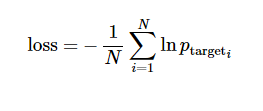
\includegraphics{../images/re.png}
\caption{}
\end{figure}

实现起来并非很难,而且函数 \lstinline{sequence\_loss\_by\_example}
已经有了,可以直接使用。

论文中的典型衡量标准是每个词语的平均困惑度(perplexity),计算式为

\begin{figure}[htbp]
\centering
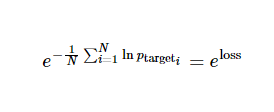
\includegraphics{../images/re1.png}
\caption{}
\end{figure}

同时我们会观察训练过程中的困惑度值(perplexity)。

\subsubsection{多个 LSTM 层堆叠
}\label{ux591aux4e2a-lstm-ux5c42ux5806ux53e0}

要想给模型更强的表达能力,可以添加多层 LSTM
来处理数据。第一层的输出作为第二层的输入,以此类推。

类 \lstinline{MultiRNNCell} 可以无缝的将其实现:

\begin{Shaded}
\begin{Highlighting}[]
\NormalTok{lstm }\OperatorTok{=} \NormalTok{rnn_cell.BasicLSTMCell(lstm_size)}
\NormalTok{stacked_lstm }\OperatorTok{=} \NormalTok{rnn_cell.MultiRNNCell([lstm] }\OperatorTok{*} \NormalTok{number_of_layers)}

\NormalTok{initial_state }\OperatorTok{=} \NormalTok{state }\OperatorTok{=} \NormalTok{stacked_lstm.zero_state(batch_size, tf.float32)}
\ControlFlowTok{for} \NormalTok{i }\OperatorTok{in} \BuiltInTok{range}\NormalTok{(}\BuiltInTok{len}\NormalTok{(num_steps)):}
    \CommentTok{# 每次处理一批词语后更新状态值.}
    \NormalTok{output, state }\OperatorTok{=} \NormalTok{stacked_lstm(words[:, i], state)}

    \CommentTok{# 其余的代码.}
    \CommentTok{# ...}

\NormalTok{final_state }\OperatorTok{=} \NormalTok{state}
\end{Highlighting}
\end{Shaded}

\subsection{编译并运行代码
}\label{ux7f16ux8bd1ux5e76ux8fd0ux884cux4ee3ux7801}

首先需要构建库,在 CPU 上编译:

\begin{verbatim}
bazel build -c opt tensorflow/models/rnn/ptb:ptb_word_lm
\end{verbatim}

如果你有一个强大的 GPU,可以运行:

\begin{verbatim}
bazel build -c opt --config=cuda tensorflow/models/rnn/ptb:ptb_word_lm
\end{verbatim}

运行模型:

\begin{verbatim}
bazel-bin/tensorflow/models/rnn/ptb/ptb_word_lm \
  --data_path=/tmp/simple-examples/data/ --alsologtostderr --model small
\end{verbatim}

教程代码中有 3 个支持的模型配置参数:``small'', ``medium'' 和
``large''。它们指的是 LSTM 的大小,以及用于训练的超参数集。

模型越大,得到的结果应该更好。在测试集中 \lstinline{small}
模型应该可以达到低于 120 的困惑度(perplexity),\lstinline{large}
模型则是低于 80,但它可能花费数小时来训练。

\subsection{除此之外? }\label{ux9664ux6b64ux4e4bux5916}

还有几个优化模型的技巧没有提到,包括:

\begin{itemize}
\tightlist
\item
  随时间降低学习率,
\item
  LSTM 层间 dropout.
\end{itemize}

继续学习和更改代码以进一步改善模型吧。

原文:\href{http://tensorflow.org/tutorials/recurrent/index.md}{Recurrent
Neural Networks} 翻译:\href{https://github.com/Warln}{Warln}
校对:\href{https://github.com/wanghong-yang}{HongyangWang}


\section{Sequence-to-Sequence Models
}\label{sequence-to-sequence-models}

Recurrent neural networks can learn to model language, as already
discussed in the
\href{tensorflow-zh/SOURCE/tutorials/recurrent/index.md}{RNN Tutorial}
(if you did not read it, please go through it before proceeding with
this one). This raises an interesting question: could we condition the
generated words on some input and generate a meaningful response? For
example, could we train a neural network to translate from English to
French? It turns out that the answer is \emph{yes}.

This tutorial will show you how to build and train such a system
end-to-end. You can start by running this binary.

\begin{verbatim}
bazel run -c opt <...>/models/rnn/translate/translate.py
  --data_dir [your_data_directory]
\end{verbatim}

It will download English-to-French translation data from the
\href{http://www.statmt.org/wmt15/translation-task.html}{WMT'15 Website}
prepare it for training and train. It takes about 20GB of disk space,
and a while to download and prepare (see
\protect\hyperlink{runux5fit}{later} for details), so you can start and
leave it running while reading this tutorial.

This tutorial references the following files from \texttt{models/rnn}.

\begin{longtable}[c]{@{}ll@{}}
\toprule
\begin{minipage}[b]{0.05\columnwidth}\raggedright\strut
File
\strut\end{minipage} &
\begin{minipage}[b]{0.05\columnwidth}\raggedright\strut
What's in it?
\strut\end{minipage}\tabularnewline
\midrule
\endhead
\begin{minipage}[t]{0.05\columnwidth}\raggedright\strut
\texttt{seq2seq.py}
\strut\end{minipage} &
\begin{minipage}[t]{0.05\columnwidth}\raggedright\strut
Library for building sequence-to-sequence models.
\strut\end{minipage}\tabularnewline
\begin{minipage}[t]{0.05\columnwidth}\raggedright\strut
\texttt{translate/seq2seq\_model.py}
\strut\end{minipage} &
\begin{minipage}[t]{0.05\columnwidth}\raggedright\strut
Neural translation sequence-to-sequence model.
\strut\end{minipage}\tabularnewline
\begin{minipage}[t]{0.05\columnwidth}\raggedright\strut
\texttt{translate/data\_utils.py}
\strut\end{minipage} &
\begin{minipage}[t]{0.05\columnwidth}\raggedright\strut
Helper functions for preparing translation data.
\strut\end{minipage}\tabularnewline
\begin{minipage}[t]{0.05\columnwidth}\raggedright\strut
\texttt{translate/translate.py}
\strut\end{minipage} &
\begin{minipage}[t]{0.05\columnwidth}\raggedright\strut
Binary that trains and runs the translation model.
\strut\end{minipage}\tabularnewline
\bottomrule
\end{longtable}

\subsection{Sequence-to-Sequence Basics
}\label{sequence-to-sequence-basics}

A basic sequence-to-sequence model, as introduced in
\href{http://arxiv.org/pdf/1406.1078v3.pdf}{Cho et al., 2014}, consists
of two recurrent neural networks (RNNs): an \emph{encoder} that
processes the input and a \emph{decoder} that generates the output. This
basic architecture is depicted below.

Each box in the picture above represents a cell of the RNN, most
commonly a GRU cell or an LSTM cell (see the
\href{tensorflow-zh/SOURCE/tutorials/recurrent/index.md}{RNN Tutorial}
for an explanation of those). Encoder and decoder can share weights or,
as is more common, use a different set of parameters. Mutli-layer cells
have been successfully used in sequence-to-sequence models too, e.g.~for
translation \href{http://arxiv.org/abs/1409.3215}{Sutskever et al.,
2014}.

In the basic model depicted above, every input has to be encoded into a
fixed-size state vector, as that is the only thing passed to the
decoder. To allow the decoder more direct access to the input, an
\emph{attention} mechanism was introduced in
\href{http://arxiv.org/abs/1409.0473}{Bahdanu et al., 2014}. We will not
go into the details of the attention mechanism (see the paper), suffice
it to say that it allows the decoder to peek into the input at every
decoding step. A multi-layer sequence-to-sequence network with LSTM
cells and attention mechanism in the decoder looks like this.

\subsection{TensorFlow seq2seq Library
}\label{tensorflow-seq2seq-library}

As you can see above, there are many different sequence-to-sequence
models. Each of these models can use different RNN cells, but all of
them accept encoder inputs and decoder inputs. This motivates the
interfaces in the TensorFlow seq2seq library
(\texttt{models/rnn/seq2seq.py}). The basic RNN encoder-decoder
sequence-to-sequence model works as follows.

\begin{Shaded}
\begin{Highlighting}[]
\NormalTok{outputs, states }\OperatorTok{=} \NormalTok{basic_rnn_seq2seq(encoder_inputs, decoder_inputs, cell)}
\end{Highlighting}
\end{Shaded}

In the above call, \texttt{encoder\_inputs} are a list of tensors
representing inputs to the encoder, i.e., corresponding to the letters
\emph{A, B, C} in the first picture above. Similarly,
\texttt{decoder\_inputs} are tensors representing inputs to the decoder,
\emph{GO, W, X, Y, Z} on the first picture.

The \texttt{cell} argument is an instance of the
\texttt{models.rnn.rnn\_cell.RNNCell} class that determines which cell
will be used inside the model. You can use an existing cell, such as
\texttt{GRUCell} or \texttt{LSTMCell}, or you can write your own.
Moreover, \texttt{rnn\_cell} provides wrappers to construct multi-layer
cells, add dropout to cell inputs or outputs, or to do other
transformations, see the
\href{tensorflow-zh/SOURCE/tutorials/recurrent/index.md}{RNN Tutorial}
for examples.

The call to \texttt{basic\_rnn\_seq2seq} returns two arguments:
\texttt{outputs} and \texttt{states}. Both of them are lists of tensors
of the same length as \texttt{decoder\_inputs}. Naturally,
\texttt{outputs} correspond to the outputs of the decoder in each
time-step, in the first picture above that would be \emph{W, X, Y, Z,
EOS}. The returned \texttt{states} represent the internal state of the
decoder at every time-step.

In many applications of sequence-to-sequence models, the output of the
decoder at time t is fed back and becomes the input of the decoder at
time t+1. At test time, when decoding a sequence, this is how the
sequence is constructed. During training, on the other hand, it is
common to provide the correct input to the decoder at every time-step,
even if the decoder made a mistake before. Functions in
\texttt{seq2seq.py} support both modes using the \texttt{feed\_previous}
argument. For example, let's analyze the following use of an embedding
RNN model.

\begin{Shaded}
\begin{Highlighting}[]
\NormalTok{outputs, states }\OperatorTok{=} \NormalTok{embedding_rnn_seq2seq(}
    \NormalTok{encoder_inputs, decoder_inputs, cell,}
    \NormalTok{num_encoder_symbols, num_decoder_symbols,}
    \NormalTok{output_projection}\OperatorTok{=}\VariableTok{None}\NormalTok{, feed_previous}\OperatorTok{=}\VariableTok{False}\NormalTok{)}
\end{Highlighting}
\end{Shaded}

In the \texttt{embedding\_rnn\_seq2seq} model, all inputs (both
\texttt{encoder\_inputs} and \texttt{decoder\_inputs}) are
integer-tensors that represent discrete values. They will be embedded
into a dense representation (see the
\href{tensorflow-zh/SOURCE/tutorials/word2vec/index.md}{Vectors
Representations Tutorial} for more details on embeddings), but to
construct these embeddings we need to specify the maximum number of
discrete symbols that will appear: \texttt{num\_encoder\_symbols} on the
encoder side, and \texttt{num\_decoder\_symbols} on the decoder side.

In the above invocation, we set \texttt{feed\_previous} to False. This
means that the decoder will use \texttt{decoder\_inputs} tensors as
provided. If we set \texttt{feed\_previous} to True, the decoder would
only use the first element of \texttt{decoder\_inputs}. All other
tensors from this list would be ignored, and instead the previous output
of the encoder would be used. This is used for decoding translations in
our translation model, but it can also be used during training, to make
the model more robust to its own mistakes, similar to
\href{http://arxiv.org/pdf/1506.03099v2.pdf}{Bengio et al., 2015}.

One more important argument used above is \texttt{output\_projection}.
If not specified, the outputs of the embedding model will be tensors of
shape batch-size by \texttt{num\_decoder\_symbols} as they represent the
logits for each generated symbol. When training models with large output
vocabularies, i.e., when \texttt{num\_decoder\_symbols} is large, it is
not practical to store these large tensors. Instead, it is better to
return smaller output tensors, which will later be projected onto a
large output tensor using \texttt{output\_projection}. This allows to
use our seq2seq models with a sampled softmax loss, as described in
\href{http://arxiv.org/pdf/1412.2007v2.pdf}{Jean et. al., 2015}.

In addition to \texttt{basic\_rnn\_seq2seq} and
\texttt{embedding\_rnn\_seq2seq} there are a few more
sequence-to-sequence models in \texttt{seq2seq.py}, take a look there.
They all have similar interfaces, so we will not describe them in
detail. We will use \texttt{embedding\_attention\_seq2seq} for our
translation model below.

\subsection{Neural Translation Model }\label{neural-translation-model}

While the core of the sequence-to-sequence model is constructed by the
functions in \texttt{models/rnn/seq2seq.py}, there are still a few
tricks that are worth mentioning that are used in our translation model
in \texttt{models/rnn/translate/seq2seq\_model.py}.

\subsubsection{Sampled softmax and output projection
}\label{sampled-softmax-and-output-projection}

For one, as already mentioned above, we want to use sampled softmax to
handle large output vocabulary. To decode from it, we need to keep track
of the output projection. Both the sampled softmax loss and the output
projections are constructed by the following code in
\texttt{seq2seq\_model.py}.

\begin{Shaded}
\begin{Highlighting}[]
  \ControlFlowTok{if} \NormalTok{num_samples }\OperatorTok{>} \DecValTok{0} \OperatorTok{and} \NormalTok{num_samples }\OperatorTok{<} \VariableTok{self}\NormalTok{.target_vocab_size:}
    \NormalTok{w }\OperatorTok{=} \NormalTok{tf.get_variable(}\StringTok{"proj_w"}\NormalTok{, [size, }\VariableTok{self}\NormalTok{.target_vocab_size])}
    \NormalTok{w_t }\OperatorTok{=} \NormalTok{tf.transpose(w)}
    \NormalTok{b }\OperatorTok{=} \NormalTok{tf.get_variable(}\StringTok{"proj_b"}\NormalTok{, [}\VariableTok{self}\NormalTok{.target_vocab_size])}
    \NormalTok{output_projection }\OperatorTok{=} \NormalTok{(w, b)}

    \KeywordTok{def} \NormalTok{sampled_loss(inputs, labels):}
      \NormalTok{labels }\OperatorTok{=} \NormalTok{tf.reshape(labels, [}\OperatorTok{-}\DecValTok{1}\NormalTok{, }\DecValTok{1}\NormalTok{])}
      \ControlFlowTok{return} \NormalTok{tf.nn.sampled_softmax_loss(w_t, b, inputs, labels, num_samples,}
                                        \VariableTok{self}\NormalTok{.target_vocab_size)}
\end{Highlighting}
\end{Shaded}

First, note that we only construct a sampled softmax if the number of
samples (512 by default) is smaller that the target vocabulary size. For
vocabularies smaller than 512 it might be a better idea to just use a
standard softmax loss.

Then, as you can see, we construct an output projection. It is a pair,
consisting of a weight matrix and a bias vector. If used, the rnn cell
will return vectors of shape batch-size by \texttt{size}, rather than
batch-size by \texttt{target\_vocab\_size}. To recover logits, we need
to multiply by the weight matrix and add the biases, as is done in lines
124-126 in \texttt{seq2seq\_model.py}.

\begin{Shaded}
\begin{Highlighting}[]
\ControlFlowTok{if} \NormalTok{output_projection }\OperatorTok{is} \OperatorTok{not} \VariableTok{None}\NormalTok{:}
  \VariableTok{self}\NormalTok{.outputs[b] }\OperatorTok{=} \NormalTok{[tf.matmul(output, output_projection[}\DecValTok{0}\NormalTok{]) }\OperatorTok{+}
                     \NormalTok{output_projection[}\DecValTok{1}\NormalTok{] }\ControlFlowTok{for} \NormalTok{...]}
\end{Highlighting}
\end{Shaded}

\subsubsection{Bucketing and padding }\label{bucketing-and-padding}

In addition to sampled softmax, our translation model also makes use of
\emph{bucketing}, which is a method to efficiently handle sentences of
different lengths. Let us first clarify the problem. When translating
English to French, we will have English sentences of different lengths
L1 on input, and French sentences of different lengths L2 on output.
Since the English sentence is passed as \texttt{encoder\_inputs}, and
the French sentence comes as \texttt{decoder\_inputs} (prefixed by a GO
symbol), we should in principle create a seq2seq model for every pair
(L1, L2+1) of lengths of an English and French sentence. This would
result in an enormous graph consisting of many very similar subgraphs.
On the other hand, we could just pad every sentence with a special PAD
symbol. Then we'd need only one seq2seq model, for the padded lengths.
But on shorter sentence our model would be inefficient, encoding and
decoding many PAD symbols that are useless.

As a compromise between contructing a graph for every pair of lengths
and padding to a single length, we use a number of \emph{buckets} and
pad each sentence to the length of the bucket above it. In
\texttt{translate.py} we use the following default buckets.

\begin{Shaded}
\begin{Highlighting}[]
\NormalTok{buckets }\OperatorTok{=} \NormalTok{[(}\DecValTok{5}\NormalTok{, }\DecValTok{10}\NormalTok{), (}\DecValTok{10}\NormalTok{, }\DecValTok{15}\NormalTok{), (}\DecValTok{20}\NormalTok{, }\DecValTok{25}\NormalTok{), (}\DecValTok{40}\NormalTok{, }\DecValTok{50}\NormalTok{)]}
\end{Highlighting}
\end{Shaded}

This means that if the input is an English sentence with 3 tokens, and
the corresponding output is a French sentence with 6 tokens, then they
will be put in the first bucket and padded to length 5 for encoder
inputs, and length 10 for decoder inputs. If we have an English sentence
with 8 tokens and the corresponding French sentence has 18 tokens, then
they will not fit into the (10, 15) bucket, and so the (20, 25) bucket
will be used, i.e.~the English sentence will be padded to 20, and the
French one to 25.

Remember that when constructing decoder inputs we prepend the special
\texttt{GO} symbol to the input data. This is done in the
\texttt{get\_batch()} function in \texttt{seq2seq\_model.py}, which also
reverses the input English sentence. Reversing the inputs was shown to
improve results for the neural translation model in
\href{http://arxiv.org/abs/1409.3215}{Sutskever et al., 2014}. To put it
all together, imagine we have the sentence ``I go.'', tokenized as
\texttt{{[}"I",\ "go",\ "."{]}} as input and the sentence ``Je vais.''
as output, tokenized \texttt{{[}"Je",\ "vais",\ "."{]}}. It will be put
in the (5, 10) bucket, with encoder inputs representing
\texttt{{[}PAD\ PAD\ "."\ "go"\ "I"{]}} and decoder inputs
\texttt{{[}GO\ "Je"\ "vais"\ "."\ EOS\ PAD\ PAD\ PAD\ PAD\ PAD{]}}.

\subsection{Let's Run It }\label{lets-run-it}

To train the model described above, we need to a large English-French
corpus. We will use the \emph{10\^{}9-French-English corpus} from the
\href{http://www.statmt.org/wmt15/translation-task.html}{WMT'15 Website}
for training, and the 2013 news test from the same site as development
set. Both data-sets will be downloaded to \texttt{data\_dir} and
training will start, saving checkpoints in \texttt{train\_dir}, when
this command is run.

\begin{verbatim}
bazel run -c opt <...>/models/rnn/translate:translate
  --data_dir [your_data_directory] --train_dir [checkpoints_directory]
  --en_vocab_size=40000 --fr_vocab_size=40000
\end{verbatim}

It takes about 18GB of disk space and several hours to prepare the
training corpus. It is unpacked, vocabulary files are created in
\texttt{data\_dir}, and then the corpus is tokenized and converted to
integer ids. Note the parameters that determine vocabulary sizes. In the
example above, all words outside the 40K most common ones will be
converted to an \texttt{UNK} token representing unknown words. So if you
change vocabulary size, the binary will re-map the corpus to token-ids
again.

After the data is prepared, training starts. Default parameters in
\texttt{translate} are set to quite large values. Large models trained
over a long time give good results, but it might take too long or use
too much memory for your GPU. You can request to train a smaller model
as in the following example.

\begin{verbatim}
bazel run -c opt <...>/models/rnn/translate:translate
  --data_dir [your_data_directory] --train_dir [checkpoints_directory]
  --size=256 --num_layers=2 --steps_per_checkpoint=50
\end{verbatim}

The above command will train a model with 2 layers (the default is 3),
each layer with 256 units (default is 1024), and will save a checkpoint
every 50 steps (the default is 200). You can play with these parameters
to find out how large a model can be to fit into the memory of your GPU.

During training, every \texttt{steps\_per\_checkpoint} steps the binary
will print out statistics from recent steps. With the default parameters
(3 layers of size 1024), first messages look like this.

\begin{verbatim}
global step 200 learning rate 0.5000 step-time 1.39 perplexity 1720.62
  eval: bucket 0 perplexity 184.97
  eval: bucket 1 perplexity 248.81
  eval: bucket 2 perplexity 341.64
  eval: bucket 3 perplexity 469.04
global step 400 learning rate 0.5000 step-time 1.38 perplexity 379.89
  eval: bucket 0 perplexity 151.32
  eval: bucket 1 perplexity 190.36
  eval: bucket 2 perplexity 227.46
  eval: bucket 3 perplexity 238.66
\end{verbatim}

You can see that each step takes just under 1.4 seconds, the perplexity
on the training set and the perplexities on the development set for each
bucket. After about 30K steps, we see perplexities on short sentences
(bucket 0 and 1) going into single digits. Since the training corpus
contains \textasciitilde{}22M sentences, one epoch (going through the
training data once) takes about 340K steps with batch-size of 64. At
this point the model can be used for translating English sentences to
French using the \texttt{-\/-decode} option.

\begin{verbatim}
bazel run -c opt <...>/models/rnn/translate:translate --decode
  --data_dir [your_data_directory] --train_dir [checkpoints_directory]

Reading model parameters from /tmp/translate.ckpt-340000
>  Who is the president of the United States?
 Qui est le président des États-Unis ?
\end{verbatim}

\subsection{What Next? }\label{what-next}

The example above shows how you can build your own English-to-French
translator, end-to-end. Run it and see how the model performs for
yourself. While it has reasonable quality, the default parameters will
not give you the best translation model. Here are a few things you can
improve.

First of all, we use a very promitive tokenizer, the
\texttt{basic\_tokenizer} function in \texttt{data\_utils}. A better
tokenizer can be found on the
\href{http://www.statmt.org/wmt15/translation-task.html}{WMT'15
Website}. Using that tokenizer, and a larger vocabulary, should improve
your translations.

Also, the default parameters of the translation model are not tuned. You
can try changing the learning rate, decay, or initializing the weights
of your model in a different way. You can also change the default
\texttt{GradientDescentOptimizer} in \texttt{seq2seq\_model.py} to a
more advanced one, such as \texttt{AdagradOptimizer}. Try these things
and see how they improve your results!

Finally, the model presented above can be used for any
sequence-to-sequence task, not only for translation. Even if you want to
transform a sequence to a tree, for example to generate a parsing tree,
the same model as above can give state-of-the-art results, as
demonstrated in \href{http://arxiv.org/abs/1412.7449}{Vinyals \& Kaiser
et al., 2015}. So you can not only build your own translator, you can
also build a parser, a chat-bot, or any program that comes to your mind.
Experiment!
\include{tutorials/c2s08_mandelbrot}


\section{偏微分方程 }\label{ux504fux5faeux5206ux65b9ux7a0b}

\textbf{\emph{TensorFlow}}
不仅仅是用来机器学习,它更可以用来模拟仿真。在这里,我们将通过模拟仿真几滴落入一块方形水池的雨点的例子,来引导您如何使用
\textbf{\emph{TensorFlow}} 中的偏微分方程来模拟仿真的基本使用方法。

\begin{quote}
注:本教程最初是准备做为一个 \textbf{IPython} 的手册。
\textgreater{}译者注:关于偏微分方程的相关知识,译者推荐读者查看
\href{http://open.163.com/}{\textbf{网易公开课}}
上的\href{http://open.163.com/special/opencourse/multivariable.html}{\textbf{《麻省理工学院公开课:多变量微积分》}}课程。
\end{quote}

\subsection{基本设置 }\label{ux57faux672cux8bbeux7f6e}

首先,我们需要导入一些必要的引用。

\begin{Shaded}
\begin{Highlighting}[]
\CommentTok{#导入模拟仿真需要的库}
\ImportTok{import} \NormalTok{tensorflow }\ImportTok{as} \NormalTok{tf}
\ImportTok{import} \NormalTok{numpy }\ImportTok{as} \NormalTok{np}

\CommentTok{#导入可视化需要的库}
\ImportTok{import} \NormalTok{PIL.Image}
\ImportTok{from} \NormalTok{cStringIO }\ImportTok{import} \NormalTok{StringIO}
\ImportTok{from} \NormalTok{IPython.display }\ImportTok{import} \NormalTok{clear_output, Image, display}
\end{Highlighting}
\end{Shaded}

然后,我们还需要一个用于表示池塘表面状态的函数。

\begin{Shaded}
\begin{Highlighting}[]
\KeywordTok{def} \NormalTok{DisplayArray(a, fmt}\OperatorTok{=}\StringTok{'jpeg'}\NormalTok{, rng}\OperatorTok{=}\NormalTok{[}\DecValTok{0}\NormalTok{,}\DecValTok{1}\NormalTok{]):}
  \CommentTok{"""Display an array as a picture."""}
  \NormalTok{a }\OperatorTok{=} \NormalTok{(a }\OperatorTok{-} \NormalTok{rng[}\DecValTok{0}\NormalTok{])}\OperatorTok{/}\BuiltInTok{float}\NormalTok{(rng[}\DecValTok{1}\NormalTok{] }\OperatorTok{-} \NormalTok{rng[}\DecValTok{0}\NormalTok{])}\OperatorTok{*}\DecValTok{255}
  \NormalTok{a }\OperatorTok{=} \NormalTok{np.uint8(np.clip(a, }\DecValTok{0}\NormalTok{, }\DecValTok{255}\NormalTok{))}
  \NormalTok{f }\OperatorTok{=} \NormalTok{StringIO()}
  \NormalTok{PIL.Image.fromarray(a).save(f, fmt)}
  \NormalTok{display(Image(data}\OperatorTok{=}\NormalTok{f.getvalue()))}
\end{Highlighting}
\end{Shaded}

最后,为了方便演示,这里我们需要打开一个 \textbf{\emph{TensorFlow}}
的交互会话(interactive
session)。当然为了以后能方便调用,我们可以把相关代码写到一个可以执行的\textbf{\emph{Python}}文件中。

\begin{Shaded}
\begin{Highlighting}[]
\NormalTok{sess }\OperatorTok{=} \NormalTok{tf.InteractiveSession()}
\end{Highlighting}
\end{Shaded}

\subsection{定义计算函数 }\label{ux5b9aux4e49ux8ba1ux7b97ux51fdux6570}

\begin{Shaded}
\begin{Highlighting}[]
\KeywordTok{def} \NormalTok{make_kernel(a):}
  \CommentTok{"""Transform a 2D array into a convolution kernel"""}
  \NormalTok{a }\OperatorTok{=} \NormalTok{np.asarray(a)}
  \NormalTok{a }\OperatorTok{=} \NormalTok{a.reshape(}\BuiltInTok{list}\NormalTok{(a.shape) }\OperatorTok{+} \NormalTok{[}\DecValTok{1}\NormalTok{,}\DecValTok{1}\NormalTok{])}
  \ControlFlowTok{return} \NormalTok{tf.constant(a, dtype}\OperatorTok{=}\DecValTok{1}\NormalTok{)}

\KeywordTok{def} \NormalTok{simple_conv(x, k):}
  \CommentTok{"""A simplified 2D convolution operation"""}
  \NormalTok{x }\OperatorTok{=} \NormalTok{tf.expand_dims(tf.expand_dims(x, }\DecValTok{0}\NormalTok{), }\OperatorTok{-}\DecValTok{1}\NormalTok{)}
  \NormalTok{y }\OperatorTok{=} \NormalTok{tf.nn.depthwise_conv2d(x, k, [}\DecValTok{1}\NormalTok{, }\DecValTok{1}\NormalTok{, }\DecValTok{1}\NormalTok{, }\DecValTok{1}\NormalTok{], padding}\OperatorTok{=}\StringTok{'SAME'}\NormalTok{)}
  \ControlFlowTok{return} \NormalTok{y[}\DecValTok{0}\NormalTok{, :, :, }\DecValTok{0}\NormalTok{]}

\KeywordTok{def} \NormalTok{laplace(x):}
  \CommentTok{"""Compute the 2D laplacian of an array"""}
  \NormalTok{laplace_k }\OperatorTok{=} \NormalTok{make_kernel([[}\FloatTok{0.5}\NormalTok{, }\FloatTok{1.0}\NormalTok{, }\FloatTok{0.5}\NormalTok{],}
                           \NormalTok{[}\FloatTok{1.0}\NormalTok{, }\OperatorTok{-}\DecValTok{6}\NormalTok{., }\FloatTok{1.0}\NormalTok{],}
                           \NormalTok{[}\FloatTok{0.5}\NormalTok{, }\FloatTok{1.0}\NormalTok{, }\FloatTok{0.5}\NormalTok{]])}
  \ControlFlowTok{return} \NormalTok{simple_conv(x, laplace_k)}
\end{Highlighting}
\end{Shaded}

\subsection{定义偏微分方程
}\label{ux5b9aux4e49ux504fux5faeux5206ux65b9ux7a0b}

首先,我们需要创建一个完美的 500 × 500
的正方形池塘,就像是我们在现实中找到的一样。

\begin{Shaded}
\begin{Highlighting}[]
\NormalTok{N }\OperatorTok{=} \DecValTok{500}
\end{Highlighting}
\end{Shaded}

然后,我们需要创建了一个池塘和几滴将要坠入池塘的雨滴。

\begin{Shaded}
\begin{Highlighting}[]
\CommentTok{# Initial Conditions -- some rain drops hit a pond}

\CommentTok{# Set everything to zero}
\NormalTok{u_init }\OperatorTok{=} \NormalTok{np.zeros([N, N], dtype}\OperatorTok{=}\StringTok{"float32"}\NormalTok{)}
\NormalTok{ut_init }\OperatorTok{=} \NormalTok{np.zeros([N, N], dtype}\OperatorTok{=}\StringTok{"float32"}\NormalTok{)}

\CommentTok{# Some rain drops hit a pond at random points}
\ControlFlowTok{for} \NormalTok{n }\OperatorTok{in} \BuiltInTok{range}\NormalTok{(}\DecValTok{40}\NormalTok{):}
  \NormalTok{a,b }\OperatorTok{=} \NormalTok{np.random.randint(}\DecValTok{0}\NormalTok{, N, }\DecValTok{2}\NormalTok{)}
  \NormalTok{u_init[a,b] }\OperatorTok{=} \NormalTok{np.random.uniform()}

\NormalTok{DisplayArray(u_init, rng}\OperatorTok{=}\NormalTok{[}\OperatorTok{-}\FloatTok{0.1}\NormalTok{, }\FloatTok{0.1}\NormalTok{])}
\end{Highlighting}
\end{Shaded}

\begin{figure}[htbp]
\centering

\includegraphics{../images/pde_output_1.jpg}
\caption{jpeg}
\end{figure}

现在,让我们来指定该微分方程的一些详细参数。

\begin{Shaded}
\begin{Highlighting}[]
\CommentTok{# Parameters:}
\CommentTok{# eps -- time resolution}
\CommentTok{# damping -- wave damping}
\NormalTok{eps }\OperatorTok{=} \NormalTok{tf.placeholder(tf.float32, shape}\OperatorTok{=}\NormalTok{())}
\NormalTok{damping }\OperatorTok{=} \NormalTok{tf.placeholder(tf.float32, shape}\OperatorTok{=}\NormalTok{())}

\CommentTok{# Create variables for simulation state}
\NormalTok{U  }\OperatorTok{=} \NormalTok{tf.Variable(u_init)}
\NormalTok{Ut }\OperatorTok{=} \NormalTok{tf.Variable(ut_init)}

\CommentTok{# Discretized PDE update rules}
\NormalTok{U_ }\OperatorTok{=} \NormalTok{U }\OperatorTok{+} \NormalTok{eps }\OperatorTok{*} \NormalTok{Ut}
\NormalTok{Ut_ }\OperatorTok{=} \NormalTok{Ut }\OperatorTok{+} \NormalTok{eps }\OperatorTok{*} \NormalTok{(laplace(U) }\OperatorTok{-} \NormalTok{damping }\OperatorTok{*} \NormalTok{Ut)}

\CommentTok{# Operation to update the state}
\NormalTok{step }\OperatorTok{=} \NormalTok{tf.group(}
  \NormalTok{U.assign(U_),}
  \NormalTok{Ut.assign(Ut_))}
\end{Highlighting}
\end{Shaded}

\subsection{开始仿真 }\label{ux5f00ux59cbux4effux771f}

为了能看清仿真效果,我们可以用一个简单的 \textbf{for}
循环来远行我们的仿真程序。

\begin{Shaded}
\begin{Highlighting}[]
\CommentTok{# Initialize state to initial conditions}
\NormalTok{tf.initialize_all_variables().run()}

\CommentTok{# Run 1000 steps of PDE}
\ControlFlowTok{for} \NormalTok{i }\OperatorTok{in} \BuiltInTok{range}\NormalTok{(}\DecValTok{1000}\NormalTok{):}
  \CommentTok{# Step simulation}
  \NormalTok{step.run(\{eps: }\FloatTok{0.03}\NormalTok{, damping: }\FloatTok{0.04}\NormalTok{\})}
  \CommentTok{# Visualize every 50 steps}
  \ControlFlowTok{if} \NormalTok{i }\OperatorTok{%} \DecValTok{50} \OperatorTok{==} \DecValTok{0}\NormalTok{:}
    \NormalTok{clear_output()}
    \NormalTok{DisplayArray(U.}\BuiltInTok{eval}\NormalTok{(), rng}\OperatorTok{=}\NormalTok{[}\OperatorTok{-}\FloatTok{0.1}\NormalTok{, }\FloatTok{0.1}\NormalTok{])}
\end{Highlighting}
\end{Shaded}

\begin{figure}[htbp]
\centering

\includegraphics{../images/pde_output_2.jpg}
\caption{jpeg}
\end{figure}

看!! 雨点落在池塘中,和现实中一样的泛起了涟漪。

\begin{quote}
原文链接:\url{http://tensorflow.org/tutorials/pdes/index.md}
翻译:{[}@wangaicc{]}(https://github.com/wangaicc)
校对:{[}@tensorfly{]}(https://github.com/tensorfly)
\end{quote}


\section{MNIST 数据下载 }\label{mnist-ux6570ux636eux4e0bux8f7d}

源码:
\href{https://tensorflow.googlesource.com/tensorflow/+/master/tensorflow/g3doc/tutorials/mnist/}{tensorflow/g3doc/tutorials/mnist/}

本教程的目标是展示如何下载用于手写数字分类问题所要用到的(经典)MNIST数据集。

\subsection{教程 文件 }\label{ux6559ux7a0b-ux6587ux4ef6}

本教程需要使用以下文件:

\begin{longtable}[c]{@{}ll@{}}
\toprule
\begin{minipage}[b]{0.05\columnwidth}\raggedright\strut
文件
\strut\end{minipage} &
\begin{minipage}[b]{0.05\columnwidth}\raggedright\strut
目的
\strut\end{minipage}\tabularnewline
\midrule
\endhead
\begin{minipage}[t]{0.05\columnwidth}\raggedright\strut
\href{https://tensorflow.googlesource.com/tensorflow/+/master/tensorflow/g3doc/tutorials/mnist/input_data.py}{\texttt{input\_data.py}}
\strut\end{minipage} &
\begin{minipage}[t]{0.05\columnwidth}\raggedright\strut
下载用于训练和测试的MNIST数据集的源码
\strut\end{minipage}\tabularnewline
\bottomrule
\end{longtable}

\subsection{准备数据 }\label{ux51c6ux5907ux6570ux636e}

MNIST是在机器学习领域中的一个经典问题。该问题解决的是把28x28像素的灰度手写数字图片识别为相应的数字,其中数字的范围从0到9.

\begin{figure}[htbp]
\centering

\includegraphics{../images/mnist_digits.png}
\caption{MNIST Digits}
\end{figure}

更多详情, 请参考 \href{http://yann.lecun.com/exdb/mnist/}{Yann LeCun's
MNIST page} 或
\href{http://colah.github.io/posts/2014-10-Visualizing-MNIST/}{Chris
Olah's visualizations of MNIST}.

\subsubsection{下载 }\label{ux4e0bux8f7d}

\href{http://yann.lecun.com/exdb/mnist/}{Yann LeCun's MNIST page}
也提供了训练集与测试集数据的下载。

\begin{longtable}[c]{@{}ll@{}}
\toprule
\begin{minipage}[b]{0.05\columnwidth}\raggedright\strut
文件
\strut\end{minipage} &
\begin{minipage}[b]{0.05\columnwidth}\raggedright\strut
内容
\strut\end{minipage}\tabularnewline
\midrule
\endhead
\begin{minipage}[t]{0.05\columnwidth}\raggedright\strut
\href{http://yann.lecun.com/exdb/mnist/train-images-idx3-ubyte.gz}{\texttt{train-images-idx3-ubyte.gz}}
\strut\end{minipage} &
\begin{minipage}[t]{0.05\columnwidth}\raggedright\strut
训练集图片 - 55000 张 训练图片, 5000 张 验证图片
\strut\end{minipage}\tabularnewline
\begin{minipage}[t]{0.05\columnwidth}\raggedright\strut
\href{http://yann.lecun.com/exdb/mnist/train-labels-idx1-ubyte.gz}{\texttt{train-labels-idx1-ubyte.gz}}
\strut\end{minipage} &
\begin{minipage}[t]{0.05\columnwidth}\raggedright\strut
训练集图片对应的数字标签
\strut\end{minipage}\tabularnewline
\begin{minipage}[t]{0.05\columnwidth}\raggedright\strut
\href{http://yann.lecun.com/exdb/mnist/t10k-images-idx3-ubyte.gz}{\texttt{t10k-images-idx3-ubyte.gz}}
\strut\end{minipage} &
\begin{minipage}[t]{0.05\columnwidth}\raggedright\strut
测试集图片 - 10000 张 图片
\strut\end{minipage}\tabularnewline
\begin{minipage}[t]{0.05\columnwidth}\raggedright\strut
\href{http://yann.lecun.com/exdb/mnist/t10k-labels-idx1-ubyte.gz}{\texttt{t10k-labels-idx1-ubyte.gz}}
\strut\end{minipage} &
\begin{minipage}[t]{0.05\columnwidth}\raggedright\strut
测试集图片对应的数字标签
\strut\end{minipage}\tabularnewline
\bottomrule
\end{longtable}

在 \texttt{input\_data.py} 文件中, \texttt{maybe\_download()}
函数可以确保这些训练数据下载到本地文件夹中。

文件夹的名字在 \texttt{fully\_connected\_feed.py}
文件的顶部由一个标记变量指定,你可以根据自己的需要进行修改。 \#\#\# 解压
与 重构

这些文件本身并没有使用标准的图片格式储存,并且需要使用\texttt{input\_data.py}文件中\texttt{extract\_images()}
和\texttt{extract\_labels()}函数来手动解压(页面中有相关说明)。

图片数据将被解压成2维的tensor:\texttt{{[}image\ index,\ pixel\ index{]}}
其中每一项表示某一图片中特定像素的强度值, 范围从 \texttt{{[}0,\ 255{]}}
到 \texttt{{[}-0.5,\ 0.5{]}}。 ``image index''代表数据集中图片的编号,
从0到数据集的上限值。``pixel index''代表该图片中像素点得个数,
从0到图片的像素上限值。

以\texttt{train-*}开头的文件中包括60000个样本,其中分割出55000个样本作为训练集,其余的5000个样本作为验证集。因为所有数据集中28x28像素的灰度图片的尺寸为784,所以训练集输出的tensor格式为\texttt{{[}55000,\ 784{]}}。

数字标签数据被解压称1维的tensor:
\texttt{{[}image\ index{]}},它定义了每个样本数值的类别分类。对于训练集的标签来说,这个数据规模就是:\texttt{{[}55000{]}}。

\subsubsection{数据集 对象 }\label{ux6570ux636eux96c6-ux5bf9ux8c61}

底层的源码将会执行下载、解压、重构图片和标签数据来组成以下的数据集对象:

\begin{longtable}[c]{@{}ll@{}}
\toprule
数据集 & 目的\tabularnewline
\midrule
\endhead
\texttt{data\_sets.train} & 55000 组 图片和标签,
用于训练。\tabularnewline
\texttt{data\_sets.validation} & 5000 组 图片和标签,
用于迭代验证训练的准确性。\tabularnewline
\texttt{data\_sets.test} & 10000 组 图片和标签,
用于最终测试训练的准确性。\tabularnewline
\bottomrule
\end{longtable}

执行\texttt{read\_data\_sets()}函数将会返回一个\texttt{DataSet}实例,其中包含了以上三个数据集。函数\texttt{DataSet.next\_batch()}是用于获取以\texttt{batch\_size}为大小的一个元组,其中包含了一组图片和标签,该元组会被用于当前的TensorFlow运算会话中。

\begin{Shaded}
\begin{Highlighting}[]
\NormalTok{images_feed, labels_feed }\OperatorTok{=} \NormalTok{data_set.next_batch(FLAGS.batch_size)}
\end{Highlighting}
\end{Shaded}

原文地址:\href{https://github.com/tensorflow/tensorflow/blob/master/tensorflow/g3doc/tutorials/mnist/download/index.md}{MNIST
Data Download} 翻译:\href{https://github.com/btpeter}{btpeter}
校对:waiwaizheng


\newpage
% Chapter 3 How to...
% 第三章 运作方式
\chapter{运作方式}


% \section{综述 Overview}\label{ux7efcux8ff0-overview}

综述 Overview

\subsection{Variables:
创建,初始化,保存,和恢复}\label{variables-ux521bux5efaux521dux59cbux5316ux4fddux5b58ux548cux6062ux590d}

TensorFlow Variables 是内存中的容纳 tensor
的缓存。这一小节介绍了用它们在模型训练时(during
training)创建、保存和更新模型参数(model parameters) 的方法。

\href{../how_tos/variables.md}{参看教程}

\subsection{TensorFlow 机制 101}\label{tensorflow-ux673aux5236-101}

用 MNIST 手写数字识别作为一个小例子,一步一步的将使用 TensorFlow
基础架构(infrastructure)训练大规模模型的细节做详细介绍。

\href{../tutorials/mnist_tf.md}{参看教程}

\subsection{TensorBoard:
学习过程的可视化}\label{tensorboard-ux5b66ux4e60ux8fc7ux7a0bux7684ux53efux89c6ux5316}

对模型进行训练和评估时,TensorBoard
是一个很有用的可视化工具。此教程解释了创建和运行 TensorBoard
的方法,和使用摘要操作(Summary ops)的方法,通过添加摘要操作(Summary
ops),可以自动把数据传输到 TensorBoard 所使用的事件文件。

\href{../how_tos/summaries_and_tensorboard.md}{参看教程}

\subsection{TensorBoard:
图的可视化}\label{tensorboard-ux56feux7684ux53efux89c6ux5316}

此教程介绍了在 TensorBoard
中使用可视化工具的方法,它可以帮助你理解张量流图的过程并 debug。

\href{../how_tos/graph_viz.md}{参看教程}

\subsection{数据读入}\label{ux6570ux636eux8bfbux5165}

此教程介绍了把数据传入 TensorSlow 程序的三种主要的方法: Feeding,
Reading 和 Preloading.

\href{../how_tos/reading_data.md}{参看教程}

\subsection{线程和队列}\label{ux7ebfux7a0bux548cux961fux5217}

此教程介绍 TensorFlow
中为了更容易进行异步和并发训练的各种不同结构(constructs)。

\href{../how_tos/threading_and_queues.md}{参看教程}

\subsection{添加新的 Op}\label{ux6dfbux52a0ux65b0ux7684-op}

TensorFlow 已经提供一整套节点操作()operation),你可以在你的 graph
中随意使用它们,不过这里有关于添加自定义操作(custom op)的细节。

\href{../how_tos/adding_an_op.md}{参看教程}。

\subsection{自定义数据的
Readers}\label{ux81eaux5b9aux4e49ux6570ux636eux7684-readers}

如果你有相当大量的自定义数据集合,可能你想要对 TensorFlow 的 Data
Readers 进行扩展,使它能直接以数据自身的格式将其读入。

\href{../how_tos/new_data_formats.md}{参看教程}。

\subsection{使用 GPUs}\label{ux4f7fux7528-gpus}

此教程描述了用多个 GPU 构建和运行模型的方法。

\href{../how_tos/using_gpu.md}{参看教程}

\subsection{共享变量 Sharing
Variables}\label{ux5171ux4eabux53d8ux91cf-sharing-variables}

当在多 GPU 上部署大型的模型,或展开复杂的 LSTMs 或 RNNs
时,在模型构建代码的不同位置对许多相同的变量(Variable)进行读写常常是必须的。设计变量作用域(Variable
Scope)机制的目的就是为了帮助上述任务的实现。

\href{../how_tos/variable_scope/index.md}{参看教程}。

原文: \href{http://tensorflow.org/how_tos/index.html}{How-to}

翻译:\href{https://github.com/TerenceCooper}{Terence Cooper}

校对:\href{https://github.com/lonlonago}{lonlonago}
%!TEX program = xelatex
% Encoding: UTF8
% SEIKA 2015


% Chapter 3 How to ...
% Section 3.1



\section{变量:创建、初始化、保存和加载}

当训练模型时,用变量来存储和更新参数。变量包含张量 (Tensor)存放于内存的缓存区。建模时它们需要被明确地初始化,模型训练后它们必须被存储到磁盘。这些变量的值可在之后模型训练和分析是被加载。

本文档描述以下两个TensorFlow类。点击以下链接可查看完整的API文档:
\begin{itemize}
  \item tf.Variable 类 % add link here
  \item tf.train.Saver 类 % add link here
\end{itemize}

\subsection {变量创建}

当创建一个变量时,你将一个张量作为初始值传入构造函数Variable()。TensorFlow提供了一系列操作符来初始化张量,初始值是常量或是随机值。
% add link here

\begin{lstlisting}
# Create two variables.
weights = tf.Variable(tf.random_normal([784, 200], stddev=0.35), name="weights")
biases = tf.Variable(tf.zeros([200]), name="biases")
\end{lstlisting}

调用tf.Variable()添加一些操作(Op, operation)到graph:
\begin{itemize}
  \item 一个Variable操作存放变量的值。
  \item 一个初始化op将变量设置为初始值。这事实上是一个tf.assign操作。
  \item 初始值的操作,例如示例中对biases变量的zeros操作也被加入了graph。
\end{itemize}
\lstinline{tf.Variable}的返回值是Python的\lstinline{tf.Variable}类的一个实例。

\subsection {变量初始化}

变量的初始化必须在模型的其它操作运行之前先明确地完成。最简单的方法就是添加一个给所有变量初始化的操作,并在使用模型之前首先运行那个操作。

你或者可以从检查点文件中重新获取变量值,详见下文。

使用\lstinline{tf.initialize_all_variables()}添加一个操作对变量做初始化。记得在完全构建好模型并加载之后再运行那个操作。

\begin{lstlisting}
# Create two variables.
weights = tf.Variable(tf.random_normal([784, 200], stddev=0.35),
                      name="weights")
biases = tf.Variable(tf.zeros([200]), name="biases")
...
# Add an op to initialize the variables.
init_op = tf.initialize_all_variables()

# Later, when launching the model
with tf.Session() as sess:
  # Run the init operation.
  sess.run(init_op)
  ...
  # Use the model
  ...
\end{lstlisting}

\subsubsection{由另一个变量初始化}
你有时候会需要用另一个变量的初始化值给当前变量初始化。由于\lstinline{tf.initialize_all_variables()}是并行地初始化所有变量,所以在有这种需求的情况下需要小心。

用其它变量的值初始化一个新的变量时,使用其它变量的\lstinline{initialized_value()}属性。你可以直接把已初始化的值作为新变量的初始值,或者把它当做tensor计算得到一个值赋予新变量。

\begin{lstlisting}
# Create a variable with a random value.
weights = tf.Variable(tf.random_normal([784, 200], stddev=0.35),name="weights")
# Create another variable with the same value as 'weights'.
w2 = tf.Variable(weights.initialized_value(), name="w2")
# Create another variable with twice the value of 'weights'
w_twice = tf.Variable(weights.initialized_value() * 0.2, name="w_twice")
\end{lstlisting}

\subsubsection{自定义初始化}

\lstinline{tf.initialize_all_variables()}函数便捷地添加一个op来初始化模型的所有变量。你也可以给它传入一组变量进行初始化。详情请见Variables Documentation,包括检查变量是否被初始化。

% add link of Variables Documentaion here
\subsection {保存和加载}
最简单的保存和恢复模型的方法是使用\lseinline{tf.train.Saver}对象。构造器给graph的所有变量,或是定义在列表里的变量,添加\lstinline{save}和\lstinline{restoreops}。\lstinline{saver}对象提供了方法来运行这些ops,定义检查点文件的读写路径。

\subsubsection{Checkpoint Files}
Variables are saved in binary files that, roughly, contain a map from variable names to tensor values.

When you create a Saver object, you can optionally choose names for the variables in the checkpoint files. By default, it uses the value of the \lstinline{Variable.name} property for each variable.
% add link of Variable.name here
% https://www.tensorflow.org/versions/master/api_docs/python/state_ops.html#Variable.name

\subsubsection{保存变量}

用\lstinline{tf.train.Saver()}创建一个\lstinline{Saver}来管理模型中的所有变量。

\begin{lstlisting}
# Create some variables.
v1 = tf.Variable(..., name="v1")
v2 = tf.Variable(..., name="v2")
...
# Add an op to initialize the variables.
init_op = tf.initialize_all_variables()

# Add ops to save and restore all the variables.
saver = tf.train.Saver()

# Later, launch the model, initialize the variables, do some work, save the
# variables to disk.
with tf.Session() as sess:
  sess.run(init_op)
  # Do some work with the model.
  ..
  # Save the variables to disk.
  save_path = saver.save(sess, "/tmp/model.ckpt")
  print "Model saved in file: ", save_path
\end{lstlisting}

\subsubsection{恢复变量}

用同一个\lstinline{Saver}对象来恢复变量。注意,当你从文件中恢复变量时,不需要事先对它们做初始化。

\begin{lstlisting}
# Create some variables.
v1 = tf.Variable(..., name="v1")
v2 = tf.Variable(..., name="v2")
...
# Add ops to save and restore all the variables.
saver = tf.train.Saver()

# Later, launch the model, use the saver to restore variables from disk, and
# do some work with the model.
with tf.Session() as sess:
  # Restore variables from disk.
  saver.restore(sess, "/tmp/model.ckpt")
  print "Model restored."
  # Do some work with the model
  ...
\end{lstlisting}

\subsubsection{选择存储和恢复哪些变量}
如果你不给\lstinline{tf.train.Saver()}传入任何参数,那么\lstinline{saver}将处理\lstinline{graph}中的所有变量。其中每一个变量都以变量创建时传入的名称被保存。

有时候在检查点文件中明确定义变量的名称很有用。举个例子,你也许已经训练得到了一个模型,其中有个变量命名为\lstinline{"weights"},你想把它的值恢复到一个新的变量\lstinline{"params"}中。

有时候仅保存和恢复模型的一部分变量很有用。再举个例子,你也许训练得到了一个5层神经网络,现在想训练一个6层的新模型,可以将之前5层模型的参数导入到新模型的前5层中。

你可以通过给\lstinline{tf.train.Saver()}构造函数传入Python字典,很容易地定义需要保持的变量及对应名称:键对应使用的名称,值对应被管理的变量。

\textbf{注意}:

\begin{quote}
You can create as many saver objects as you want if you need to save and restore different subsets of the model variables. The same variable can be listed in multiple saver objects, its value is only changed when the saver restore() method is run.

If you only restore a subset of the model variables at the start of a session, you have to run an initialize op for the other variables. See \lstinline{tf.initialize_variables()} for more information.
\end{quote}

如果需要保存和恢复模型变量的不同子集,可以创建任意多个saver对象。同一个变量可被列入多个saver对象中,只有当saver的\lstinline{restore()}函数被运行时,它的值才会发生改变。

如果你仅在session开始时恢复模型变量的一个子集,你需要对剩下的变量执行初始化op。详情请见\lstinline{tf.initialize_variables()}。

% add link of tf.initialize_variables() here
% https://www.tensorflow.org/versions/master/api_docs/python/state_ops.html#initialize_variables

\begin{lstlisting}
# Create some variables.
v1 = tf.Variable(..., name="v1")
v2 = tf.Variable(..., name="v2")
...
# Add ops to save and restore only 'v2' using the name "my_v2"
saver = tf.train.Saver({"my_v2": v2})
# Use the saver object normally after that.
...
\end{lstlisting}


\section{共享变量}\label{ux5171ux4eabux53d8ux91cf}

你可以在\href{tensorflow-zh/SOURCE/how_tos/variables/index.md}{怎么使用变量}中所描述的方式来创建,初始化,保存及加载单一的变量.但是当创建复杂的模块时,通常你需要共享大量变量集并且如果你还想在同一个地方初始化这所有的变量,我们又该怎么做呢.本教程就是演示如何使用\texttt{tf.variable\_scope()}
和\texttt{tf.get\_variable()}两个方法来实现这一点.

\subsection{问题}\label{ux95eeux9898}

假设你为图片过滤器创建了一个简单的模块,和我们的\href{tensorflow-zh/SOURCE/tutorials/deep_cnn/index.md}{卷积神经网络教程}模块相似,但是这里包括两个卷积(为了简化实例这里只有两个).如果你仅使用\texttt{tf.Variable}变量,那么你的模块就如\href{tensorflow-zh/SOURCE/how_tos/variables/index.md}{怎么使用变量}里面所解释的是一样的模块.

\begin{Shaded}
\begin{Highlighting}[]
\KeywordTok{def} \NormalTok{my_image_filter(input_images):}
    \NormalTok{conv1_weights }\OperatorTok{=} \NormalTok{tf.Variable(tf.random_normal([}\DecValTok{5}\NormalTok{, }\DecValTok{5}\NormalTok{, }\DecValTok{32}\NormalTok{, }\DecValTok{32}\NormalTok{]),}
        \NormalTok{name}\OperatorTok{=}\StringTok{"conv1_weights"}\NormalTok{)}
    \NormalTok{conv1_biases }\OperatorTok{=} \NormalTok{tf.Variable(tf.zeros([}\DecValTok{32}\NormalTok{]), name}\OperatorTok{=}\StringTok{"conv1_biases"}\NormalTok{)}
    \NormalTok{conv1 }\OperatorTok{=} \NormalTok{tf.nn.conv2d(input_images, conv1_weights,}
        \NormalTok{strides}\OperatorTok{=}\NormalTok{[}\DecValTok{1}\NormalTok{, }\DecValTok{1}\NormalTok{, }\DecValTok{1}\NormalTok{, }\DecValTok{1}\NormalTok{], padding}\OperatorTok{=}\StringTok{'SAME'}\NormalTok{)}
    \NormalTok{relu1 }\OperatorTok{=} \NormalTok{tf.nn.relu(conv1 }\OperatorTok{+} \NormalTok{conv1_biases)}

    \NormalTok{conv2_weights }\OperatorTok{=} \NormalTok{tf.Variable(tf.random_normal([}\DecValTok{5}\NormalTok{, }\DecValTok{5}\NormalTok{, }\DecValTok{32}\NormalTok{, }\DecValTok{32}\NormalTok{]),}
        \NormalTok{name}\OperatorTok{=}\StringTok{"conv2_weights"}\NormalTok{)}
    \NormalTok{conv2_biases }\OperatorTok{=} \NormalTok{tf.Variable(tf.zeros([}\DecValTok{32}\NormalTok{]), name}\OperatorTok{=}\StringTok{"conv2_biases"}\NormalTok{)}
    \NormalTok{conv2 }\OperatorTok{=} \NormalTok{tf.nn.conv2d(relu1, conv2_weights,}
        \NormalTok{strides}\OperatorTok{=}\NormalTok{[}\DecValTok{1}\NormalTok{, }\DecValTok{1}\NormalTok{, }\DecValTok{1}\NormalTok{, }\DecValTok{1}\NormalTok{], padding}\OperatorTok{=}\StringTok{'SAME'}\NormalTok{)}
    \ControlFlowTok{return} \NormalTok{tf.nn.relu(conv2 }\OperatorTok{+} \NormalTok{conv2_biases)}
\end{Highlighting}
\end{Shaded}

你很容易想到,模块集很快就比一个模块变得更为复杂,仅在这里我们就有了四个不同的变量:\texttt{conv1\_weights},\texttt{conv1\_biases},
\texttt{conv2\_weights}, 和\texttt{conv2\_biases}.
当我们想重用这个模块时问题还在增多.假设你想把你的图片过滤器运用到两张不同的图片,
\texttt{image1}和\texttt{image2}.你想通过拥有同一个参数的同一个过滤器来过滤两张图片,你可以调用\texttt{my\_image\_filter()}两次,但是这会产生两组变量.

\begin{Shaded}
\begin{Highlighting}[]
\CommentTok{# First call creates one set of variables.}
\NormalTok{result1 }\OperatorTok{=} \NormalTok{my_image_filter(image1)}
\CommentTok{# Another set is created in the second call.}
\NormalTok{result2 }\OperatorTok{=} \NormalTok{my_image_filter(image2)}
\end{Highlighting}
\end{Shaded}

通常共享变量的方法就是在单独的代码块中来创建他们并且通过使用他们的函数.如使用字典的例子:

\begin{Shaded}
\begin{Highlighting}[]
\NormalTok{variables_dict }\OperatorTok{=} \NormalTok{\{}
    \StringTok{"conv1_weights"}\NormalTok{: tf.Variable(tf.random_normal([}\DecValTok{5}\NormalTok{, }\DecValTok{5}\NormalTok{, }\DecValTok{32}\NormalTok{, }\DecValTok{32}\NormalTok{]),}
        \NormalTok{name}\OperatorTok{=}\StringTok{"conv1_weights"}\NormalTok{)}
    \CommentTok{"conv1_biases"}\NormalTok{: tf.Variable(tf.zeros([}\DecValTok{32}\NormalTok{]), name}\OperatorTok{=}\StringTok{"conv1_biases"}\NormalTok{)}
    \NormalTok{... etc. ...}
\NormalTok{\}}

\KeywordTok{def} \NormalTok{my_image_filter(input_images, variables_dict):}
    \NormalTok{conv1 }\OperatorTok{=} \NormalTok{tf.nn.conv2d(input_images, variables_dict[}\StringTok{"conv1_weights"}\NormalTok{],}
        \NormalTok{strides}\OperatorTok{=}\NormalTok{[}\DecValTok{1}\NormalTok{, }\DecValTok{1}\NormalTok{, }\DecValTok{1}\NormalTok{, }\DecValTok{1}\NormalTok{], padding}\OperatorTok{=}\StringTok{'SAME'}\NormalTok{)}
    \NormalTok{relu1 }\OperatorTok{=} \NormalTok{tf.nn.relu(conv1 }\OperatorTok{+} \NormalTok{variables_dict[}\StringTok{"conv1_biases"}\NormalTok{])}

    \NormalTok{conv2 }\OperatorTok{=} \NormalTok{tf.nn.conv2d(relu1, variables_dict[}\StringTok{"conv2_weights"}\NormalTok{],}
        \NormalTok{strides}\OperatorTok{=}\NormalTok{[}\DecValTok{1}\NormalTok{, }\DecValTok{1}\NormalTok{, }\DecValTok{1}\NormalTok{, }\DecValTok{1}\NormalTok{], padding}\OperatorTok{=}\StringTok{'SAME'}\NormalTok{)}
    \ControlFlowTok{return} \NormalTok{tf.nn.relu(conv2 }\OperatorTok{+} \NormalTok{variables_dict[}\StringTok{"conv2_biases"}\NormalTok{])}

\CommentTok{# The 2 calls to my_image_filter() now use the same variables}
\NormalTok{result1 }\OperatorTok{=} \NormalTok{my_image_filter(image1, variables_dict)}
\NormalTok{result2 }\OperatorTok{=} \NormalTok{my_image_filter(image2, variables_dict)}
\end{Highlighting}
\end{Shaded}

虽然使用上面的方式创建变量是很方便的,但是在这个模块代码之外却破坏了其封装性:

\begin{itemize}
\tightlist
\item
  在构建试图的代码中标明变量的名字,类型,形状来创建.
\item
  当代码改变了,调用的地方也许就会产生或多或少或不同类型的变量.
\end{itemize}

解决此类问题的方法之一就是使用类来创建模块,在需要的地方使用类来小心地管理他们需要的变量.
一个更高明的做法,不用调用类,而是利用TensorFlow 提供了\emph{变量作用域}
机制,当构建一个视图时,很容易就可以共享命名过的变量.

\subsection{变量作用域实例}\label{ux53d8ux91cfux4f5cux7528ux57dfux5b9eux4f8b}

变量作用域机制在TensorFlow中主要由两部分组成:

\begin{itemize}
\tightlist
\item
  \texttt{tf.get\_variable(\textless{}name\textgreater{},\ \textless{}shape\textgreater{},\ \textless{}initializer\textgreater{})}:
  通过所给的名字创建或是返回一个变量.
\item
  \texttt{tf.variable\_scope(\textless{}scope\_name\textgreater{})}:
  通过 \texttt{tf.get\_variable()}为变量名指定命名空间.
\end{itemize}

方法 \texttt{tf.get\_variable()}
用来获取或创建一个变量,而不是直接调用\texttt{tf.Variable}.它采用的不是像`tf.Variable这样直接获取值来初始化的方法.一个初始化就是一个方法,创建其形状并且为这个形状提供一个张量.这里有一些在TensorFlow中使用的初始化变量:

\begin{itemize}
\tightlist
\item
  \texttt{tf.constant\_initializer(value)} 初始化一切所提供的值,
\item
  \texttt{tf.random\_uniform\_initializer(a,\ b)}从a到b均匀初始化,
\item
  \texttt{tf.random\_normal\_initializer(mean,\ stddev)}
  用所给平均值和标准差初始化均匀分布.
\end{itemize}

为了了解\texttt{tf.get\_variable()}怎么解决前面所讨论的问题,让我们在单独的方法里面创建一个卷积来重构一下代码,命名为\texttt{conv\_relu}:

\begin{Shaded}
\begin{Highlighting}[]
\KeywordTok{def} \NormalTok{conv_relu(}\BuiltInTok{input}\NormalTok{, kernel_shape, bias_shape):}
    \CommentTok{# Create variable named "weights".}
    \NormalTok{weights }\OperatorTok{=} \NormalTok{tf.get_variable(}\StringTok{"weights"}\NormalTok{, kernel_shape,}
        \NormalTok{initializer}\OperatorTok{=}\NormalTok{tf.random_normal_initializer())}
    \CommentTok{# Create variable named "biases".}
    \NormalTok{biases }\OperatorTok{=} \NormalTok{tf.get_variable(}\StringTok{"biases"}\NormalTok{, bias_shape,}
        \NormalTok{initializer}\OperatorTok{=}\NormalTok{tf.constant_intializer(}\FloatTok{0.0}\NormalTok{))}
    \NormalTok{conv }\OperatorTok{=} \NormalTok{tf.nn.conv2d(}\BuiltInTok{input}\NormalTok{, weights,}
        \NormalTok{strides}\OperatorTok{=}\NormalTok{[}\DecValTok{1}\NormalTok{, }\DecValTok{1}\NormalTok{, }\DecValTok{1}\NormalTok{, }\DecValTok{1}\NormalTok{], padding}\OperatorTok{=}\StringTok{'SAME'}\NormalTok{)}
    \ControlFlowTok{return} \NormalTok{tf.nn.relu(conv }\OperatorTok{+} \NormalTok{biases)}
\end{Highlighting}
\end{Shaded}

这个方法中用了\texttt{"weights"}
和\texttt{"biases"}两个简称.而我们更偏向于用\texttt{conv1} 和
\texttt{conv2}这两个变量的写法,但是不同的变量需要不同的名字.这就是\texttt{tf.variable\_scope()}
变量起作用的地方.他为变量指定了相应的命名空间.

\begin{Shaded}
\begin{Highlighting}[]
\KeywordTok{def} \NormalTok{my_image_filter(input_images):}
    \ControlFlowTok{with} \NormalTok{tf.variable_scope(}\StringTok{"conv1"}\NormalTok{):}
        \CommentTok{# Variables created here will be named "conv1/weights", "conv1/biases".}
        \NormalTok{relu1 }\OperatorTok{=} \NormalTok{conv_relu(input_images, [}\DecValTok{5}\NormalTok{, }\DecValTok{5}\NormalTok{, }\DecValTok{32}\NormalTok{, }\DecValTok{32}\NormalTok{], [}\DecValTok{32}\NormalTok{])}
    \ControlFlowTok{with} \NormalTok{tf.variable_scope(}\StringTok{"conv2"}\NormalTok{):}
        \CommentTok{# Variables created here will be named "conv2/weights", "conv2/biases".}
        \ControlFlowTok{return} \NormalTok{conv_relu(relu1, [}\DecValTok{5}\NormalTok{, }\DecValTok{5}\NormalTok{, }\DecValTok{32}\NormalTok{, }\DecValTok{32}\NormalTok{], [}\DecValTok{32}\NormalTok{])}
\end{Highlighting}
\end{Shaded}

现在,让我们看看当我们调用 \texttt{my\_image\_filter()}
两次时究竟会发生了什么.

\begin{verbatim}
result1 = my_image_filter(image1)
result2 = my_image_filter(image2)
# Raises ValueError(... conv1/weights already exists ...)
\end{verbatim}

就像你看见的一样,\texttt{tf.get\_variable()}会检测已经存在的变量是否已经共享.如果你想共享他们,你需要像下面使用的一样,通过\texttt{reuse\_variables()}这个方法来指定.

\begin{verbatim}
with tf.variable_scope("image_filters") as scope:
    result1 = my_image_filter(image1)
    scope.reuse_variables()
    result2 = my_image_filter(image2)
\end{verbatim}

用这种方式来共享变量是非常好的,轻量级而且安全.

\subsection{变量作用域是怎么工作的?}\label{ux53d8ux91cfux4f5cux7528ux57dfux662fux600eux4e48ux5de5ux4f5cux7684}

\subsubsection{\texorpdfstring{理解 \texttt{tf.get\_variable()}
}{理解 tf.get\_variable() }}\label{ux7406ux89e3-tf.getux5fvariable}

为了理解变量作用域,首先完全理解\texttt{tf.get\_variable()}是怎么工作的是很有必要的.
通常我们就是这样调用\texttt{tf.get\_variable} 的.

\begin{Shaded}
\begin{Highlighting}[]
\NormalTok{v }\OperatorTok{=} \NormalTok{tf.get_variable(name, shape, dtype, initializer)}
\end{Highlighting}
\end{Shaded}

此调用做了有关作用域的两件事中的其中之一,方法调入.总的有两种情况.

\begin{itemize}
\tightlist
\item
  情况1:当\texttt{tf.get\_variable\_scope().reuse\ ==\ False}时,作用域就是为创建新变量所设置的.
\end{itemize}

这种情况下,\texttt{v}将通过\texttt{tf.Variable}所提供的形状和数据类型来重新创建.创建变量的全称将会由当前变量作用域名+所提供的\texttt{名字}所组成,并且还会检查来确保没有任何变量使用这个全称.如果这个全称已经有一个变量使用了,那么方法将会抛出\texttt{ValueError}错误.如果一个变量被创建,他将会用\texttt{initializer(shape)}进行初始化.比如:

\begin{Shaded}
\begin{Highlighting}[]
\ControlFlowTok{with} \NormalTok{tf.variable_scope(}\StringTok{"foo"}\NormalTok{):}
    \NormalTok{v }\OperatorTok{=} \NormalTok{tf.get_variable(}\StringTok{"v"}\NormalTok{, [}\DecValTok{1}\NormalTok{])}
\ControlFlowTok{assert} \NormalTok{v.name }\OperatorTok{==} \StringTok{"foo/v:0"}
\end{Highlighting}
\end{Shaded}

\begin{itemize}
\tightlist
\item
  情况1:当\texttt{tf.get\_variable\_scope().reuse\ ==\ True}时,作用域是为重用变量所设置
\end{itemize}

这种情况下,调用就会搜索一个已经存在的变量,他的全称和当前变量的作用域名+所提供的\texttt{名字}是否相等.如果不存在相应的变量,就会抛出\texttt{ValueError}
错误.如果变量找到了,就返回这个变量.如下:

\begin{Shaded}
\begin{Highlighting}[]
\ControlFlowTok{with} \NormalTok{tf.variable_scope(}\StringTok{"foo"}\NormalTok{):}
    \NormalTok{v }\OperatorTok{=} \NormalTok{tf.get_variable(}\StringTok{"v"}\NormalTok{, [}\DecValTok{1}\NormalTok{])}
\ControlFlowTok{with} \NormalTok{tf.variable_scope(}\StringTok{"foo"}\NormalTok{, reuse}\OperatorTok{=}\VariableTok{True}\NormalTok{):}
    \NormalTok{v1 }\OperatorTok{=} \NormalTok{tf.get_variable(}\StringTok{"v"}\NormalTok{, [}\DecValTok{1}\NormalTok{])}
\ControlFlowTok{assert} \NormalTok{v1 }\OperatorTok{==} \NormalTok{v}
\end{Highlighting}
\end{Shaded}

\subsubsection{\texorpdfstring{\texttt{tf.variable\_scope()}
基础}{tf.variable\_scope() 基础}}\label{tf.variableux5fscope-ux57faux7840}

知道\texttt{tf.get\_variable()}是怎么工作的,使得理解变量作用域变得很容易.变量作用域的主方法带有一个名称,它将会作为前缀用于变量名,并且带有一个重用标签来区分以上的两种情况.嵌套的作用域附加名字所用的规则和文件目录的规则很类似:

\begin{Shaded}
\begin{Highlighting}[]
\ControlFlowTok{with} \NormalTok{tf.variable_scope(}\StringTok{"foo"}\NormalTok{):}
    \ControlFlowTok{with} \NormalTok{tf.variable_scope(}\StringTok{"bar"}\NormalTok{):}
        \NormalTok{v }\OperatorTok{=} \NormalTok{tf.get_variable(}\StringTok{"v"}\NormalTok{, [}\DecValTok{1}\NormalTok{])}
\ControlFlowTok{assert} \NormalTok{v.name }\OperatorTok{==} \StringTok{"foo/bar/v:0"}
\end{Highlighting}
\end{Shaded}

当前变量作用域可以用\texttt{tf.get\_variable\_scope()}进行检索并且\texttt{reuse}
标签可以通过调用\texttt{tf.get\_variable\_scope().reuse\_variables()}设置为\texttt{True}
.

\begin{Shaded}
\begin{Highlighting}[]
\ControlFlowTok{with} \NormalTok{tf.variable_scope(}\StringTok{"foo"}\NormalTok{):}
    \NormalTok{v }\OperatorTok{=} \NormalTok{tf.get_variable(}\StringTok{"v"}\NormalTok{, [}\DecValTok{1}\NormalTok{])}
    \NormalTok{tf.get_variable_scope().reuse_variables()}
    \NormalTok{v1 }\OperatorTok{=} \NormalTok{tf.get_variable(}\StringTok{"v"}\NormalTok{, [}\DecValTok{1}\NormalTok{])}
\ControlFlowTok{assert} \NormalTok{v1 }\OperatorTok{==} \NormalTok{v}
\end{Highlighting}
\end{Shaded}

注意你\emph{不能}设置\texttt{reuse}标签为\texttt{False}.其中的原因就是允许改写创建模块的方法.想一下你前面写得方法\texttt{my\_image\_filter(inputs)}.有人在变量作用域内调用\texttt{reuse=True}
是希望所有内部变量都被重用.如果允许在方法体内强制执行\texttt{reuse=False},将会打破内部结构并且用这种方法使得很难再共享参数.

即使你不能直接设置 \texttt{reuse} 为 \texttt{False}
,但是你可以输入一个重用变量作用域,然后就释放掉,就成为非重用的变量.当打开一个变量作用域时,使用\texttt{reuse=True}
作为参数是可以的.但也要注意,同一个原因,\texttt{reuse}
参数是不可继承.所以当你打开一个重用变量作用域,那么所有的子作用域也将会被重用.

\begin{Shaded}
\begin{Highlighting}[]
\ControlFlowTok{with} \NormalTok{tf.variable_scope(}\StringTok{"root"}\NormalTok{):}
    \CommentTok{# At start, the scope is not reusing.}
    \ControlFlowTok{assert} \NormalTok{tf.get_variable_scope().reuse }\OperatorTok{==} \VariableTok{False}
    \ControlFlowTok{with} \NormalTok{tf.variable_scope(}\StringTok{"foo"}\NormalTok{):}
        \CommentTok{# Opened a sub-scope, still not reusing.}
        \ControlFlowTok{assert} \NormalTok{tf.get_variable_scope().reuse }\OperatorTok{==} \VariableTok{False}
    \ControlFlowTok{with} \NormalTok{tf.variable_scope(}\StringTok{"foo"}\NormalTok{, reuse}\OperatorTok{=}\VariableTok{True}\NormalTok{):}
        \CommentTok{# Explicitly opened a reusing scope.}
        \ControlFlowTok{assert} \NormalTok{tf.get_variable_scope().reuse }\OperatorTok{==} \VariableTok{True}
        \ControlFlowTok{with} \NormalTok{tf.variable_scope(}\StringTok{"bar"}\NormalTok{):}
            \CommentTok{# Now sub-scope inherits the reuse flag.}
            \ControlFlowTok{assert} \NormalTok{tf.get_variable_scope().reuse }\OperatorTok{==} \VariableTok{True}
    \CommentTok{# Exited the reusing scope, back to a non-reusing one.}
    \ControlFlowTok{assert} \NormalTok{tf.get_variable_scope().reuse }\OperatorTok{==} \VariableTok{False}
\end{Highlighting}
\end{Shaded}

\subsubsection{获取变量作用域}\label{ux83b7ux53d6ux53d8ux91cfux4f5cux7528ux57df}

在上面的所有例子中,我们共享参数只因为他们的名字是一致的,那是因为我们开启一个变量作用域重用时刚好用了同一个字符串.在更复杂的情况,他可以通过变量作用域对象来使用,而不是通过依赖于右边的名字来使用.为此,变量作用域可以被获取并使用,而不是仅作为当开启一个新的变量作用域的名字.

\begin{Shaded}
\begin{Highlighting}[]
\ControlFlowTok{with} \NormalTok{tf.variable_scope(}\StringTok{"foo"}\NormalTok{) }\ImportTok{as} \NormalTok{foo_scope:}
    \NormalTok{v }\OperatorTok{=} \NormalTok{tf.get_variable(}\StringTok{"v"}\NormalTok{, [}\DecValTok{1}\NormalTok{])}
\ControlFlowTok{with} \NormalTok{tf.variable_scope(foo_scope)}
    \NormalTok{w }\OperatorTok{=} \NormalTok{tf.get_variable(}\StringTok{"w"}\NormalTok{, [}\DecValTok{1}\NormalTok{])}
\ControlFlowTok{with} \NormalTok{tf.variable_scope(foo_scope, reuse}\OperatorTok{=}\VariableTok{True}\NormalTok{)}
    \NormalTok{v1 }\OperatorTok{=} \NormalTok{tf.get_variable(}\StringTok{"v"}\NormalTok{, [}\DecValTok{1}\NormalTok{])}
    \NormalTok{w1 }\OperatorTok{=} \NormalTok{tf.get_variable(}\StringTok{"w"}\NormalTok{, [}\DecValTok{1}\NormalTok{])}
\ControlFlowTok{assert} \NormalTok{v1 }\OperatorTok{==} \NormalTok{v}
\ControlFlowTok{assert} \NormalTok{w1 }\OperatorTok{==} \NormalTok{w}
\end{Highlighting}
\end{Shaded}

当开启一个变量作用域,使用一个预先已经存在的作用域时,我们会跳过当前变量作用域的前缀而直接成为一个完全不同的作用域.这就是我们做得完全独立的地方.

\begin{Shaded}
\begin{Highlighting}[]
\ControlFlowTok{with} \NormalTok{tf.variable_scope(}\StringTok{"foo"}\NormalTok{) }\ImportTok{as} \NormalTok{foo_scope:}
    \ControlFlowTok{assert} \NormalTok{foo_scope.name }\OperatorTok{==} \StringTok{"foo"}
\ControlFlowTok{with} \NormalTok{tf.variable_scope(}\StringTok{"bar"}\NormalTok{)}
    \ControlFlowTok{with} \NormalTok{tf.variable_scope(}\StringTok{"baz"}\NormalTok{) }\ImportTok{as} \NormalTok{other_scope:}
        \ControlFlowTok{assert} \NormalTok{other_scope.name }\OperatorTok{==} \StringTok{"bar/baz"}
        \ControlFlowTok{with} \NormalTok{tf.variable_scope(foo_scope) }\ImportTok{as} \NormalTok{foo_scope2:}
            \ControlFlowTok{assert} \NormalTok{foo_scope2.name }\OperatorTok{==} \StringTok{"foo"}  \CommentTok{# Not changed.}
\end{Highlighting}
\end{Shaded}

\subsubsection{变量作用域中的初始化器}\label{ux53d8ux91cfux4f5cux7528ux57dfux4e2dux7684ux521dux59cbux5316ux5668}

使用\texttt{tf.get\_variable()}允许你重写方法来创建或者重用变量,并且可以被外部透明调用.但是如果我们想改变创建变量的初始化器那要怎么做呢?是否我们需要为所有的创建变量方法传递一个额外的参数呢?那在大多数情况下,当我们想在一个地方并且为所有的方法的所有的变量设置一个默认初始化器,那又改怎么做呢?为了解决这些问题,变量作用域可以携带一个默认的初始化器.他可以被子作用域继承并传递给\texttt{tf.get\_variable()}
调用.但是如果其他初始化器被明确地指定,那么他将会被重写.

\begin{Shaded}
\begin{Highlighting}[]
\ControlFlowTok{with} \NormalTok{tf.variable_scope(}\StringTok{"foo"}\NormalTok{, initializer}\OperatorTok{=}\NormalTok{tf.constant_initializer(}\FloatTok{0.4}\NormalTok{)):}
    \NormalTok{v }\OperatorTok{=} \NormalTok{tf.get_variable(}\StringTok{"v"}\NormalTok{, [}\DecValTok{1}\NormalTok{])}
    \ControlFlowTok{assert} \NormalTok{v.}\BuiltInTok{eval}\NormalTok{() }\OperatorTok{==} \FloatTok{0.4}  \CommentTok{# Default initializer as set above.}
    \NormalTok{w }\OperatorTok{=} \NormalTok{tf.get_variable(}\StringTok{"w"}\NormalTok{, [}\DecValTok{1}\NormalTok{], initializer}\OperatorTok{=}\NormalTok{tf.constant_initializer(}\FloatTok{0.3}\NormalTok{)):}
    \ControlFlowTok{assert} \NormalTok{w.}\BuiltInTok{eval}\NormalTok{() }\OperatorTok{==} \FloatTok{0.3}  \CommentTok{# Specific initializer overrides the default.}
    \ControlFlowTok{with} \NormalTok{tf.variable_scope(}\StringTok{"bar"}\NormalTok{):}
        \NormalTok{v }\OperatorTok{=} \NormalTok{tf.get_variable(}\StringTok{"v"}\NormalTok{, [}\DecValTok{1}\NormalTok{])}
        \ControlFlowTok{assert} \NormalTok{v.}\BuiltInTok{eval}\NormalTok{() }\OperatorTok{==} \FloatTok{0.4}  \CommentTok{# Inherited default initializer.}
    \ControlFlowTok{with} \NormalTok{tf.variable_scope(}\StringTok{"baz"}\NormalTok{, initializer}\OperatorTok{=}\NormalTok{tf.constant_initializer(}\FloatTok{0.2}\NormalTok{)):}
        \NormalTok{v }\OperatorTok{=} \NormalTok{tf.get_variable(}\StringTok{"v"}\NormalTok{, [}\DecValTok{1}\NormalTok{])}
        \ControlFlowTok{assert} \NormalTok{v.}\BuiltInTok{eval}\NormalTok{() }\OperatorTok{==} \FloatTok{0.2}  \CommentTok{# Changed default initializer.}
\end{Highlighting}
\end{Shaded}

\subsubsection{\texorpdfstring{在\texttt{tf.variable\_scope()}中ops的名称}{在tf.variable\_scope()中ops的名称}}\label{ux5728tf.variableux5fscopeux4e2dopsux7684ux540dux79f0}

我们讨论 \texttt{tf.variable\_scope}
怎么处理变量的名字.但是又是如何在作用域中影响到
其他ops的名字的呢?ops在一个变量作用域的内部创建,那么他应该是共享他的名字,这是很自然的想法.出于这样的原因,当我们用\texttt{with\ tf.variable\_scope("name")}时,这就间接地开启了一个\texttt{tf.name\_scope("name")}.比如:

\begin{Shaded}
\begin{Highlighting}[]
\ControlFlowTok{with} \NormalTok{tf.variable_scope(}\StringTok{"foo"}\NormalTok{):}
    \NormalTok{x }\OperatorTok{=} \FloatTok{1.0} \OperatorTok{+} \NormalTok{tf.get_variable(}\StringTok{"v"}\NormalTok{, [}\DecValTok{1}\NormalTok{])}
\ControlFlowTok{assert} \NormalTok{x.op.name }\OperatorTok{==} \StringTok{"foo/add"}
\end{Highlighting}
\end{Shaded}

名称作用域可以被开启并添加到一个变量作用域中,然后他们只会影响到ops的名称,而不会影响到变量.

\begin{Shaded}
\begin{Highlighting}[]
\ControlFlowTok{with} \NormalTok{tf.variable_scope(}\StringTok{"foo"}\NormalTok{):}
    \ControlFlowTok{with} \NormalTok{tf.name_scope(}\StringTok{"bar"}\NormalTok{):}
        \NormalTok{v }\OperatorTok{=} \NormalTok{tf.get_variable(}\StringTok{"v"}\NormalTok{, [}\DecValTok{1}\NormalTok{])}
        \NormalTok{x }\OperatorTok{=} \FloatTok{1.0} \OperatorTok{+} \NormalTok{v}
\ControlFlowTok{assert} \NormalTok{v.name }\OperatorTok{==} \StringTok{"foo/v:0"}
\ControlFlowTok{assert} \NormalTok{x.op.name }\OperatorTok{==} \StringTok{"foo/bar/add"}
\end{Highlighting}
\end{Shaded}

当用一个引用对象而不是一个字符串去开启一个变量作用域时,我们就不会为ops改变当前的名称作用域.

\subsection{使用实例 }\label{ux4f7fux7528ux5b9eux4f8b}

这里有一些指向怎么使用变量作用域的文件.特别是,他被大量用于
\href{https://zh.wikipedia.org/wiki/\%E9\%80\%92\%E5\%BD\%92\%E7\%A5\%9E\%E7\%BB\%8F\%E7\%BD\%91\%E7\%BB\%9C}{时间递归神经网络}和\texttt{sequence-to-sequence}模型,

File \textbar{} What's in it? --- \textbar{} ---
\texttt{models/image/cifar10.py} \textbar{}图像中检测对象的模型.
\texttt{models/rnn/rnn\_cell.py} \textbar{}时间递归神经网络的元方法集.
\texttt{models/rnn/seq2seq.py}
\textbar{}为创建\texttt{sequence-to-sequence}模型的方法集.
原文:\href{http://www.tensorflow.org/how_tos/variable_scope/index.md}{Sharing
Variables}
翻译:\href{https://github.com/nb312}{nb312}校对:\href{https://github.com/jikexueyuanwiki}{Wiki}


\section{TensorBoard:可视化学习 }\label{vis_learning}

TensorBoard
涉及到的运算,通常是在训练庞大的深度神经网络中出现的复杂而又难以理解的运算。

为了更方便 TensorFlow 程序的理解、调试与优化,我们发布了一套叫做
TensorBoard 的可视化工具。你可以用 TensorBoard 来展现你的 TensorFlow
图像,绘制图像生成的定量指标图以及附加数据。

当 TensorBoard 设置完成后,它应该是这样子的:

\begin{figure}[htbp]
\centering
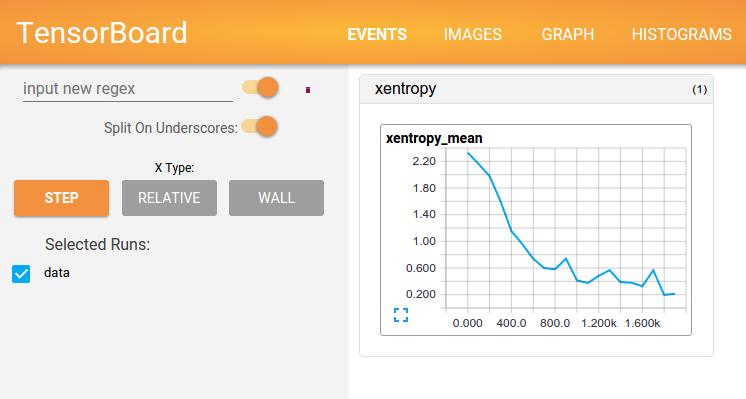
\includegraphics[width=.95\textwidth]{../SOURCE/images/mnist_tensorboard.png}
\caption{MNIST TensorBoard}
\end{figure}

\subsection{数据序列化 }\label{ux6570ux636eux5e8fux5217ux5316}

TensorBoard 通过读取 TensorFlow 的事件文件来运行。TensorFlow
的事件文件包括了你会在 TensorFlow 运行中涉及到的主要数据。下面是
TensorBoard 中汇总数据(Summary data)的大体生命周期。

首先,创建你想汇总数据的 TensorFlow
图,然后再选择你想在哪个节点进行\href{../api_docs/python/train.md\#summary_options}{汇总(summary)操作}。

比如,假设你正在训练一个卷积神经网络,用于识别 MNISt
标签。你可能希望记录学习速度(learning
rate)的如何变化,以及目标函数如何变化。通过向节点附加\href{../api_docs/python/train.md\#scalary_summary}{scalar\_summary}操作来分别输出学习速度和期望误差。然后你可以给每个
scalary\_summary 分配一个有意义的 \texttt{标签},比如
\texttt{\textquotesingle{}learning\ rate\textquotesingle{}} 和
\texttt{\textquotesingle{}loss\ function\textquotesingle{}}。

或者你还希望显示一个特殊层中激活的分布,或者梯度权重的分布。可以通过分别附加
\href{../api_docs/python/train.md\#histogram_summary}{histogram\_summary}
运算来收集权重变量和梯度输出。

所有可用的 summary
操作详细信息,可以查看\href{../api_docs/python/train.md\#summary_operation}{summary\_operation}文档。

在TensorFlow中,所有的操作只有当你执行,或者另一个操作依赖于它的输出时才会运行。我们刚才创建的这些节点(summary
nodes)都围绕着你的图像:没有任何操作依赖于它们的结果。因此,为了生成汇总信息,我们需要运行所有这些节点。这样的手动工作是很乏味的,因此可以使用\href{../api_docs/python/train.md\#scalary_summary}{tf.merge\_all\_summaries}来将他们合并为一个操作。

然后你可以执行合并命令,它会依据特点步骤将所有数据生成一个序列化的\texttt{Summary}
protobuf对象。最后,为了将汇总数据写入磁盘,需要将汇总的protobuf对象传递给\href{../api_docs/python/train.md\#SummaryWriter}{tf.train.Summarywriter}。

\texttt{SummaryWriter} 的构造函数中包含了参数 logdir。这个 logdir
非常重要,所有事件都会写到它所指的目录下。此外,\texttt{SummaryWriter}
中还包含了一个可选择的参数 \texttt{GraphDef}。如果输入了该参数,那么
TensorBoard 也会显示你的图像。

现在已经修改了你的图,也有了
\texttt{SummaryWriter},现在就可以运行你的神经网络了!如果你愿意的话,你可以每一步执行一次合并汇总,这样你会得到一大堆训练数据。这很有可能超过了你想要的数据量。你也可以每一百步执行一次合并汇总,或者如下面代码里示范的这样。

\begin{Shaded}
\begin{Highlighting}[]
\NormalTok{merged_summary_op }\OperatorTok{=} \NormalTok{tf.merge_all_summaries()}
\NormalTok{summary_writer }\OperatorTok{=} \NormalTok{tf.train.SummaryWriter(}\StringTok{'/tmp/mnist_logs'}\NormalTok{, sess.graph)}
\NormalTok{total_step }\OperatorTok{=} \DecValTok{0}
\ControlFlowTok{while} \NormalTok{training:}
  \NormalTok{total_step }\OperatorTok{+=} \DecValTok{1}
  \NormalTok{session.run(training_op)}
  \ControlFlowTok{if} \NormalTok{total_step }\OperatorTok{%} \DecValTok{100} \OperatorTok{==} \DecValTok{0}\NormalTok{:}
    \NormalTok{summary_str }\OperatorTok{=} \NormalTok{session.run(merged_summary_op)}
    \NormalTok{summary_writer.add_summary(summary_str, total_step)}
\end{Highlighting}
\end{Shaded}

现在已经准备好用 TensorBoard 来可视化这些数据了。

\subsection{启动TensorBoard }\label{ux542fux52a8tensorboard}

输入下面的指令来启动TensorBoard

\begin{verbatim}
python tensorflow/tensorboard/tensorboard.py --logdir=path/to/log-directory
\end{verbatim}

这里的参数 \texttt{logdir} 指向 \texttt{SummaryWriter}
序列化数据的存储路径。如果\texttt{logdir}目录的子目录中包含另一次运行时的数据,那么
TensorBoard 会展示所有运行的数据。一旦 TensorBoard
开始运行,你可以通过在浏览器中输入 \texttt{localhost:6006} 来查看
TensorBoard。

如果你已经通过pip安装了 TensorBoard,你可以通过执行更为简单地命令来访问
TensorBoard

\begin{verbatim}
tensorboard --logdir=/path/to/log-directory
\end{verbatim}

进入 TensorBoard
的界面时,你会在右上角看到导航选项卡,每一个选项卡将展现一组可视化的序列化数据集
。对于你查看的每一个选项卡,如果 TensorBoard
中没有数据与这个选项卡相关的话,则会显示一条提示信息指示你如何序列化相关数据。

更多更详细的关于如何使用 graph 选项来显示你的图像的信息。参见
\href{./graph_viz.md}{TensorBoard:图表可视化}

原文地址:\href{http://tensorflow.org/how_tos/summaries_and_tensorboard/index.html\#tensorboard-visualizing-learning}{TensorBoard:Visualizing
Learning} 翻译:\href{https://github.com/thylaco1eo}{thylaco1eo}
校对:\href{https://github.com/lucky521}{lucky521}




\section{TensorBoard: 图表可视化
}\label{tensorboard-ux56feux8868ux53efux89c6ux5316}

TensorFlow
图表计算强大而又复杂,图表可视化在理解和调试时显得非常有帮助。
下面是一个运作时的可式化例子。

\includegraphics{../images/graph_vis_animation.gif}
``一个TensorFlow图表的可视化'') \emph{一个TensorFlow图表的可视化。}

为了显示自己的图表,需将 TensorBoard
指向此工作的日志目录并运行,点击图表顶部窗格的标签页,然后在左上角的菜单中选择合适的运行。想要深入学习关于如何运行
TensorBoard 以及如何保证所有必要信息被记录下来,请查看
\href{tensorflow-zh/SOURCE/how_tos/summaries_and_tensorboard/index.md}{Summaries
和 TensorBoard}.

\subsection{名称域(Name scoping)和节点(Node)
}\label{ux540dux79f0ux57dfname-scopingux548cux8282ux70b9node}

典型的 TensorFlow
可以有数以千计的节点,如此多而难以一下全部看到,甚至无法使用标准图表工具来展示。为简单起见,我们为变量名划定范围,并且可视化把该信息用于在图表中的节点上定义一个层级。默认情况下,
只有顶层节点会显示。下面这个例子使用\href{tensorflow-zh/SOURCE/api_docs/python/framework.md\#name_scope}{\texttt{tf.name\_scope}}在\texttt{hidden}命名域下定义了三个操作:

\begin{Shaded}
\begin{Highlighting}[]
\ImportTok{import} \NormalTok{tensorflow }\ImportTok{as} \NormalTok{tf}

\ControlFlowTok{with} \NormalTok{tf.name_scope(}\StringTok{'hidden'}\NormalTok{) }\ImportTok{as} \NormalTok{scope:}
  \NormalTok{a }\OperatorTok{=} \NormalTok{tf.constant(}\DecValTok{5}\NormalTok{, name}\OperatorTok{=}\StringTok{'alpha'}\NormalTok{)}
  \NormalTok{W }\OperatorTok{=} \NormalTok{tf.Variable(tf.random_uniform([}\DecValTok{1}\NormalTok{, }\DecValTok{2}\NormalTok{], }\OperatorTok{-}\FloatTok{1.0}\NormalTok{, }\FloatTok{1.0}\NormalTok{), name}\OperatorTok{=}\StringTok{'weights'}\NormalTok{)}
  \NormalTok{b }\OperatorTok{=} \NormalTok{tf.Variable(tf.zeros([}\DecValTok{1}\NormalTok{]), name}\OperatorTok{=}\StringTok{'biases'}\NormalTok{)}
\end{Highlighting}
\end{Shaded}

结果是得到了下面三个操作名:

\begin{itemize}
\tightlist
\item
  \emph{hidden}/alpha
\item
  \emph{hidden}/weights
\item
  \emph{hidden}/biases
\end{itemize}

默认地,三个操作名会折叠为一个节点并标注为\texttt{hidden}。其额外细节并没有丢失,你可以双击,或点击右上方橙色的\texttt{+}来展开节点,然后就会看到三个子节点\texttt{alpha},\texttt{weights}和\texttt{biases}了。

这有一个生动的例子,例中有一个更复杂的节点,节点处于其初始和展开状态。

\begin{verbatim}
<td style="width: 50%;">
  <img src="../images/pool1_collapsed.png" alt="未展开的名称域" title="未展开的名称域" />
</td>
<td style="width: 50%;">
  <img src="../images/pool1_expanded.png" alt="展开的名称域" title="展开的名称域" />
</td>
\end{verbatim}

\begin{verbatim}
<td style="width: 50%;">
  顶级名称域的初始视图<code>pool_1</code>,点击右上方橙色的<code>+</code>按钮或双击节点来展开。
</td>
<td style="width: 50%;">
  展开的<code>pool_1</code>名称域视图,点击右上方橙色的<code>-</code>按钮或双击节点来收起此名称域。
</td>
\end{verbatim}

通过名称域把节点分组来得到可读性高的图表很关键的。如果你在构建一个模型,名称域就可以用来控制可视化结果。\textbf{你的名称域越好,可视性就越好。}

上面的图像例子说明了可视化的另一方面, TensorFlow
图表有两种连接关系:数据依赖和控制依赖。数据依赖显示两个操作之间的tensor流程,用实心箭头指示,而控制依赖用点线表示。在已展开的视图(上面的右图)中,除了用点线连接的\texttt{CheckNumerics}和\texttt{control\_dependency}之外,所有连接都是数据依赖的。

还有一种手段用来简化布局。大多数 TensorFlow
图表有一部分节点,这部分节点和其他节点之间有很多连接。比如,许多节点在初始化阶段可能会有一个控制依赖,而绘制所有\texttt{init}节点的边缘和其依赖可能会创造出一个混乱的视图。

为了减少混乱,可视化把所有 high-degree
节点分离到右边的一个\emph{从属}区域,
而不会绘制线条来表示他们的边缘。线条也不用来表示连接了,我们绘制了小\emph{节点图标}来指示这些连接关系。分离出从属节点通常不会把关键信息删除掉,因为这些节点和内构功能是相关的。

\begin{verbatim}
<td style="width: 50%;">
  <img src="../images/conv_1.png" alt="conv_1是主图表的部分" title="conv_1是主图表的部分" />
</td>
<td style="width: 50%;">
  <img src="../images/save.png" alt="save被抽出为从属节点" title="save被抽出为从属节点" />
</td>
\end{verbatim}

\begin{verbatim}
<td style="width: 50%;">
  节点<code>conv_1</code>被连接到<code>save</code>,注意其右边<code>save</code>节点图标。
</td>
<td style="width: 50%;">
  <code>save</code> has a high degree, 并会作为从属节点出现,与<code>conv_1</code>的连接作为一个节点图标显示在其左边。为了继续减少杂乱,既然<code>save</code>有很多连接,我们则只显示前5个,而把其余的缩略为<code>... 12 more</code>。
</td>
\end{verbatim}

最后一个结构上的简化法叫做\emph{序列折叠(series collapsing)}。
序列基序(Sequential
motifs)是拥有相同结构并且其名称结尾的数字不同的节点,它们被折叠进一个单独的节点块(stack)中。对长序列网络来说,序列折叠极大地简化了视图,对于已层叠的节点,双击会展开序列。

\begin{verbatim}
<td style="width: 50%;">
  <img src="../images/series.png" alt="节点序列" title="节点序列" />
</td>
<td style="width: 50%;">
  <img src="../images/series_expanded.png" alt="展开的节点序列" title="展开的节点序列" />
</td>
\end{verbatim}

\begin{verbatim}
<td style="width: 50%;">
  一个节点序列的折叠视图。
</td>
<td style="width: 50%;">
  视图的一小块, 双击后展开。
</td>
\end{verbatim}

最后,针对易读性的最后一点要说到的是,可视化为常节点和摘要节点使用了特别的图标,总结起来有下面这些节点符号:

\begin{longtable}[c]{@{}ll@{}}
\toprule
\begin{minipage}[b]{0.05\columnwidth}\raggedright\strut
符号
\strut\end{minipage} &
\begin{minipage}[b]{0.05\columnwidth}\raggedright\strut
意义
\strut\end{minipage}\tabularnewline
\midrule
\endhead
\begin{minipage}[t]{0.05\columnwidth}\raggedright\strut

\includegraphics{../images/namespace_node.png}
\strut\end{minipage} &
\begin{minipage}[t]{0.05\columnwidth}\raggedright\strut
\emph{High-level}节点代表一个名称域,双击则展开一个高层节点。
\strut\end{minipage}\tabularnewline
\begin{minipage}[t]{0.05\columnwidth}\raggedright\strut

\includegraphics{../images/horizontal_stack.png}
\strut\end{minipage} &
\begin{minipage}[t]{0.05\columnwidth}\raggedright\strut
彼此之间不连接的有限个节点序列。
\strut\end{minipage}\tabularnewline
\begin{minipage}[t]{0.05\columnwidth}\raggedright\strut

\includegraphics{../images/vertical_stack.png}
\strut\end{minipage} &
\begin{minipage}[t]{0.05\columnwidth}\raggedright\strut
彼此之间相连的有限个节点序列。
\strut\end{minipage}\tabularnewline
\begin{minipage}[t]{0.05\columnwidth}\raggedright\strut

\includegraphics{../images/op_node.png}
\strut\end{minipage} &
\begin{minipage}[t]{0.05\columnwidth}\raggedright\strut
一个单独的操作节点。
\strut\end{minipage}\tabularnewline
\begin{minipage}[t]{0.05\columnwidth}\raggedright\strut

\includegraphics{../images/constant.png}
\strut\end{minipage} &
\begin{minipage}[t]{0.05\columnwidth}\raggedright\strut
一个常量结点。
\strut\end{minipage}\tabularnewline
\begin{minipage}[t]{0.05\columnwidth}\raggedright\strut

\includegraphics{../images/summary.png}
\strut\end{minipage} &
\begin{minipage}[t]{0.05\columnwidth}\raggedright\strut
一个摘要节点。
\strut\end{minipage}\tabularnewline
\begin{minipage}[t]{0.05\columnwidth}\raggedright\strut

\includegraphics{../images/dataflow_edge.png}
\strut\end{minipage} &
\begin{minipage}[t]{0.05\columnwidth}\raggedright\strut
显示各操作间的数据流边。
\strut\end{minipage}\tabularnewline
\begin{minipage}[t]{0.05\columnwidth}\raggedright\strut

\includegraphics{../images/control_edge.png}
\strut\end{minipage} &
\begin{minipage}[t]{0.05\columnwidth}\raggedright\strut
显示各操作间的控制依赖边。
\strut\end{minipage}\tabularnewline
\begin{minipage}[t]{0.05\columnwidth}\raggedright\strut

\includegraphics{../images/reference_edge.png}
\strut\end{minipage} &
\begin{minipage}[t]{0.05\columnwidth}\raggedright\strut
引用边,表示出度操作节点可以使入度tensor发生变化。
\strut\end{minipage}\tabularnewline
\bottomrule
\end{longtable}

\subsection{交互 }\label{ux4ea4ux4e92}

通过平移和缩放来导航图表,点击和拖动用于平移,滚动手势用于缩放。双击一个节点或点击其\texttt{+}按钮来展开代表一组操作的名称域。右下角有一个小地图可以在缩放和平移时方便的改变当前视角。

要关闭一个打开的节点,再次双击它或点击它的\texttt{-}按钮,你也可以只点击一次来选中一个节点,节点的颜色会加深,并且会看到节点的详情,其连接到的节点会在可视化右上角的详情卡片显现。

\begin{verbatim}
<td style="width: 50%;">
  <img src="../images/infocard.png" alt="一个名称域的详情卡片" title="一个名称域的详情卡片" />
</td>
<td style="width: 50%;">
  <img src="../images/infocard_op.png" alt="操作节点的详情卡片" title="操作节点的详情卡片" />
</td>
\end{verbatim}

\begin{verbatim}
<td style="width: 50%;">
  详情卡片展示<code>conv2</code>名称域的详细信息,名称域中操作节点的输入和输出被结合在一起,适用于不显示属性的名称域。
</td>
<td style="width: 50%;">
  详情卡片展示<code>DecodeRaw</code>操作节点,除了输入和输出,卡片也会展示与当前节点相关的设备和属性。
</td>
\end{verbatim}

选择对于 high-degree
节点的理解也很有帮助,选择任意节点,则与它的其余连接相应的节点也会选中,这使得在进行例如查看哪一个节点是否已保存等操作时非常容易。

点击详情卡片中的一个节点名称时会选中该节点,必要的话,视角会自动平移以使该节点可见。

最后,使用图例上方的颜色菜单,你可以给你的图表选择两个颜色方案。默认的\emph{结构视图}下,当两个
high-level
节点颜色一样时,其会以相同的彩虹色彩出现,而结构唯一的节点颜色是灰色。还有一个视图则展示了不同的操作运行于什么设备之上。名称域被恰当的根据其中的操作节点的设备片件来着色。

下图是一张真实图表的图解:

\begin{verbatim}
<td style="width: 50%;">
  <img src="../images/colorby_structure.png" alt="按结构着色" title="按结构着色" />
</td>
<td style="width: 50%;">
  <img src="../images/colorby_device.png" alt="按设备着色" title="按设备着色" />
</td>
\end{verbatim}

\begin{verbatim}
<td style="width: 50%;">
  结构视图:灰色节点的结构是唯一的。橙色的<code>conv1</code>和<code>conv2</code>节点有相同的结构, 其他颜色的节点也类似。
</td>
<td style="width: 50%;">
  设备视图:名称域根据其中的操作节点的设备片件来着色,在此紫色代表GPU,绿色代表CPU。
</td>
\end{verbatim}

原文:
\href{../images/index.html\#tensorboard-graph-visualization}{TensorBoard:
Graph Visualization} 翻译: {[}@Warln{]}(https://github.com/Warln) 校对:
\href{https://github.com/lucky521}{lucky521}



\section{数据读取 }\label{ux6570ux636eux8bfbux53d6}

TensorFlow程序读取数据一共有3种方法:

\begin{itemize}
\tightlist
\item
  供给数据(Feeding): 在TensorFlow程序运行的每一步,
  让Python代码来供给数据。
\item
  从文件读取数据: 在TensorFlow图的起始,
  让一个输入管线从文件中读取数据。
\item
  预加载数据:
  在TensorFlow图中定义常量或变量来保存所有数据(仅适用于数据量比较小的情况)。
\end{itemize}

\subsection{目录}\label{ux76eeux5f55}

\subsubsection{\texorpdfstring{\protect\hyperlink{AUTOGENERATED-reading-data}{数据读取}}{数据读取}}\label{ux6570ux636eux8bfbux53d6-1}

\begin{itemize}
\tightlist
\item
  \protect\hyperlink{Feeding}{供给数据(Feeding)}
\item
  \protect\hyperlink{AUTOGENERATED-reading-from-files}{从文件读取数据}
\item
  \protect\hyperlink{AUTOGENERATED-filenames--shuffling--and-epoch-limits}{文件名,
  乱序(shuffling), 和最大训练迭代数(epoch limits)}
\item
  \protect\hyperlink{AUTOGENERATED-file-formats}{文件格式}
\item
  \protect\hyperlink{AUTOGENERATED-preprocessing}{预处理}
\item
  \protect\hyperlink{AUTOGENERATED-batching}{批处理}
\item
  \protect\hyperlink{QueueRunner}{使用\texttt{QueueRunner}创建预读线程}
\item
  \protect\hyperlink{AUTOGENERATED-filtering-records-or-producing-multiple-examples-per-record}{对记录进行过滤或者为每个纪录创建多个样本}
\item
  \protect\hyperlink{AUTOGENERATED-sparse-input-data}{序列化输入数据(Sparse
  input data)}
\item
  \protect\hyperlink{AUTOGENERATED-preloaded-data}{预加载数据}
\item
  \protect\hyperlink{AUTOGENERATED-multiple-input-pipelines}{多管线输入}
\end{itemize}

\subsection{供给数据 }\label{ux4f9bux7ed9ux6570ux636e}

TensorFlow的数据供给机制允许你在TensorFlow运算图中将数据注入到任一张量中。因此,python运算可以把数据直接设置到TensorFlow图中。

通过给run()或者eval()函数输入\texttt{feed\_dict}参数,
可以启动运算过程。

\begin{Shaded}
\begin{Highlighting}[]
\ControlFlowTok{with} \NormalTok{tf.Session():}
  \BuiltInTok{input} \OperatorTok{=} \NormalTok{tf.placeholder(tf.float32)}
  \NormalTok{classifier }\OperatorTok{=} \NormalTok{...}
  \BuiltInTok{print} \NormalTok{classifier.}\BuiltInTok{eval}\NormalTok{(feed_dict}\OperatorTok{=}\NormalTok{\{}\BuiltInTok{input}\NormalTok{: my_python_preprocessing_fn()\})}
\end{Highlighting}
\end{Shaded}

虽然你可以使用常量和变量来替换任何一个张量,
但是最好的做法应该是使用\href{tensorflow-zh/SOURCE/api_docs/python/io_ops.md\#placeholder}{\texttt{placeholder}
op}节点。设计\texttt{placeholder}节点的唯一的意图就是为了提供数据供给(feeding)的方法。\texttt{placeholder}节点被声明的时候是未初始化的,
也不包含数据, 如果没有为它供给数据, 则TensorFlow运算的时候会产生错误,
所以千万不要忘了为\texttt{placeholder}提供数据。

可以在\href{https://tensorflow.googlesource.com/tensorflow/+/master/tensorflow/g3doc/tutorials/mnist/fully_connected_feed.py}{\texttt{tensorflow/g3doc/tutorials/mnist/fully\_connected\_feed.py}}找到使用\texttt{placeholder}和MNIST训练的例子,\href{tensorflow-zh/SOURCE/tutorials/mnist/tf/index.md}{MNIST
tutorial}也讲述了这一例子。

\subsection{从文件读取数据
}\label{ux4eceux6587ux4ef6ux8bfbux53d6ux6570ux636e}

一共典型的文件读取管线会包含下面这些步骤:

\begin{enumerate}
\def\labelenumi{\arabic{enumi}.}
\tightlist
\item
  文件名列表
\item
  \emph{可配置的} 文件名乱序(shuffling)
\item
  \emph{可配置的} 最大训练迭代数(epoch limit)
\item
  文件名队列
\item
  针对输入文件格式的阅读器
\item
  纪录解析器
\item
  \emph{可配置的}预处理器
\item
  样本队列
\end{enumerate}

\subsubsection{文件名, 乱序(shuffling), 和最大训练迭代数(epoch limits)
}\label{ux6587ux4ef6ux540d-ux4e71ux5e8fshuffling-ux548cux6700ux5927ux8badux7ec3ux8fedux4ee3ux6570epoch-limits}

可以使用字符串张量(比如\texttt{{[}"file0",\ "file1"{]}},
\texttt{{[}("file\%d"\ \%\ i)\ for\ i\ in\ range(2){]}},
\texttt{{[}("file\%d"\ \%\ i)\ for\ i\ in\ range(2){]}})
或者\href{tensorflow-zh/SOURCE/api_docs/python/io_ops.md\#match_filenames_once}{\texttt{tf.train.match\_filenames\_once}
函数}来产生文件名列表。

将文件名列表交给\href{tensorflow-zh/SOURCE/api_docs/python/io_ops.md\#string_input_producer}{\texttt{tf.train.string\_input\_producer}
函数}.\texttt{string\_input\_producer}来生成一个先入先出的队列,
文件阅读器会需要它来读取数据。

\texttt{string\_input\_producer}
提供的可配置参数来设置文件名乱序和最大的训练迭代数,
\texttt{QueueRunner}会为每次迭代(epoch)将所有的文件名加入文件名队列中,
如果\texttt{shuffle=True}的话,
会对文件名进行乱序处理。这一过程是比较均匀的,因此它可以产生均衡的文件名队列。

这个\texttt{QueueRunner}的工作线程是独立于文件阅读器的线程,
因此乱序和将文件名推入到文件名队列这些过程不会阻塞文件阅读器运行。

\subsubsection{文件格式 }\label{ux6587ux4ef6ux683cux5f0f}

根据你的文件格式, 选择对应的文件阅读器,
然后将文件名队列提供给阅读器的\texttt{read}方法。阅读器的\texttt{read}方法会输出一个key来表征输入的文件和其中的纪录(对于调试非常有用),同时得到一个字符串标量,
这个字符串标量可以被一个或多个解析器,或者转换操作将其解码为张量并且构造成为样本。

\paragraph{CSV 文件 }\label{csv-ux6587ux4ef6}

从CSV文件中读取数据,
需要使用\href{tensorflow-zh/SOURCE/api_docs/python/io_ops.md\#TextLineReader}{\texttt{TextLineReader}}和\href{tensorflow-zh/SOURCE/api_docs/python/io_ops.md\#decode_csv}{\texttt{decode\_csv}}
操作, 如下面的例子所示:

\begin{Shaded}
\begin{Highlighting}[]
\NormalTok{filename_queue }\OperatorTok{=} \NormalTok{tf.train.string_input_producer([}\StringTok{"file0.csv"}\NormalTok{, }\StringTok{"file1.csv"}\NormalTok{])}

\NormalTok{reader }\OperatorTok{=} \NormalTok{tf.TextLineReader()}
\NormalTok{key, value }\OperatorTok{=} \NormalTok{reader.read(filename_queue)}

\CommentTok{# Default values, in case of empty columns. Also specifies the type of the}
\CommentTok{# decoded result.}
\NormalTok{record_defaults }\OperatorTok{=} \NormalTok{[[}\DecValTok{1}\NormalTok{], [}\DecValTok{1}\NormalTok{], [}\DecValTok{1}\NormalTok{], [}\DecValTok{1}\NormalTok{], [}\DecValTok{1}\NormalTok{]]}
\NormalTok{col1, col2, col3, col4, col5 }\OperatorTok{=} \NormalTok{tf.decode_csv(}
    \NormalTok{value, record_defaults}\OperatorTok{=}\NormalTok{record_defaults)}
\NormalTok{features }\OperatorTok{=} \NormalTok{tf.concat(}\DecValTok{0}\NormalTok{, [col1, col2, col3, col4])}

\ControlFlowTok{with} \NormalTok{tf.Session() }\ImportTok{as} \NormalTok{sess:}
  \CommentTok{# Start populating the filename queue.}
  \NormalTok{coord }\OperatorTok{=} \NormalTok{tf.train.Coordinator()}
  \NormalTok{threads }\OperatorTok{=} \NormalTok{tf.train.start_queue_runners(coord}\OperatorTok{=}\NormalTok{coord)}

  \ControlFlowTok{for} \NormalTok{i }\OperatorTok{in} \BuiltInTok{range}\NormalTok{(}\DecValTok{1200}\NormalTok{):}
    \CommentTok{# Retrieve a single instance:}
    \NormalTok{example, label }\OperatorTok{=} \NormalTok{sess.run([features, col5])}

  \NormalTok{coord.request_stop()}
  \NormalTok{coord.join(threads)}
\end{Highlighting}
\end{Shaded}

每次\texttt{read}的执行都会从文件中读取一行内容, \texttt{decode\_csv}
操作会解析这一行内容并将其转为张量列表。如果输入的参数有缺失,\texttt{record\_default}参数可以根据张量的类型来设置默认值。

在调用\texttt{run}或者\texttt{eval}去执行\texttt{read}之前,
你必须调用\texttt{tf.train.start\_queue\_runners}来将文件名填充到队列。否则\texttt{read}操作会被阻塞到文件名队列中有值为止。

\paragraph{固定长度的记录
}\label{ux56faux5b9aux957fux5ea6ux7684ux8bb0ux5f55}

从二进制文件中读取固定长度纪录,
可以使用\href{tensorflow-zh/SOURCE/api_docs/python/io_ops.md\#FixedLengthRecordReader}{\texttt{tf.FixedLengthRecordReader}}的\href{tensorflow-zh/SOURCE/api_docs/python/io_ops.md\#decode_raw}{\texttt{tf.decode\_raw}}操作。\texttt{decode\_raw}操作可以讲一个字符串转换为一个uint8的张量。

举例来说,\href{http://www.cs.toronto.edu/~kriz/cifar.html}{the CIFAR-10
dataset}的文件格式定义是:每条记录的长度都是固定的,一个字节的标签,后面是3072字节的图像数据。uint8的张量的标准操作就可以从中获取图像片并且根据需要进行重组。
例子代码可以在\href{https://tensorflow.googlesource.com/tensorflow/+/master/tensorflow/models/image/cifar10/cifar10_input.py}{\texttt{tensorflow/models/image/cifar10/cifar10\_input.py}}找到,具体讲述可参见\href{tensorflow-zh/SOURCE/tutorials/deep_cnn/index.md\#prepare-the-data}{教程}.

\paragraph{标准TensorFlow格式
}\label{ux6807ux51c6tensorflowux683cux5f0f}

另一种保存记录的方法可以允许你讲任意的数据转换为TensorFlow所支持的格式,
这种方法可以使TensorFlow的数据集更容易与网络应用架构相匹配。这种建议的方法就是使用TFRecords文件,TFRecords文件包含了\href{https://tensorflow.googlesource.com/tensorflow/+/master/tensorflow/core/example/example.proto}{\texttt{tf.train.Example}
协议内存块(protocol buffer)}(协议内存块包含了字段
\href{https://tensorflow.googlesource.com/tensorflow/+/master/tensorflow/core/example/feature.proto}{\texttt{Features}})。你可以写一段代码获取你的数据,
将数据填入到\texttt{Example}协议内存块(protocol
buffer),将协议内存块序列化为一个字符串,
并且通过\href{tensorflow-zh/SOURCE/api_docs/python/python_io.md\#TFRecordWriter}{\texttt{tf.python\_io.TFRecordWriter}
class}写入到TFRecords文件。\href{https://tensorflow.googlesource.com/tensorflow/+/master/tensorflow/g3doc/how_tos/reading_data/convert_to_records.py}{\texttt{tensorflow/g3doc/how\_tos/reading\_data/convert\_to\_records.py}}就是这样的一个例子。

从TFRecords文件中读取数据,
可以使用\href{tensorflow-zh/SOURCE/api_docs/python/io_ops.md\#TFRecordReader}{\texttt{tf.TFRecordReader}}的\href{tensorflow-zh/SOURCE/api_docs/python/io_ops.md\#parse_single_example}{\texttt{tf.parse\_single\_example}}解析器。这个\texttt{parse\_single\_example}操作可以将\texttt{Example}协议内存块(protocol
buffer)解析为张量。 MNIST的例子就使用了\texttt{convert\_to\_records}
所构建的数据。
请参看\href{https://tensorflow.googlesource.com/tensorflow/+/master/tensorflow/g3doc/how_tos/reading_data/fully_connected_reader.py}{\texttt{tensorflow/g3doc/how\_tos/reading\_data/fully\_connected\_reader.py}},
您也可以将这个例子跟\texttt{fully\_connected\_feed}的版本加以比较。

\subsubsection{预处理 }\label{ux9884ux5904ux7406}

你可以对输入的样本进行任意的预处理, 这些预处理不依赖于训练参数,
你可以在\href{https://tensorflow.googlesource.com/tensorflow/+/master/tensorflow/models/image/cifar10/cifar10.py}{\texttt{tensorflow/models/image/cifar10/cifar10.py}}找到数据归一化,
提取随机数据片,增加噪声或失真等等预处理的例子。

\subsubsection{批处理 }\label{ux6279ux5904ux7406}

在数据输入管线的末端,
我们需要有另一个队列来执行输入样本的训练,评价和推理。因此我们使用\href{tensorflow-zh/SOURCE/api_docs/python/io_ops.md\#shuffle_batch}{\texttt{tf.train.shuffle\_batch}
函数}来对队列中的样本进行乱序处理

示例:

\begin{verbatim}
def read_my_file_format(filename_queue):
  reader = tf.SomeReader()
  key, record_string = reader.read(filename_queue)
  example, label = tf.some_decoder(record_string)
  processed_example = some_processing(example)
  return processed_example, label

def input_pipeline(filenames, batch_size, num_epochs=None):
  filename_queue = tf.train.string_input_producer(
      filenames, num_epochs=num_epochs, shuffle=True)
  example, label = read_my_file_format(filename_queue)
  # min_after_dequeue defines how big a buffer we will randomly sample
  #   from -- bigger means better shuffling but slower start up and more
  #   memory used.
  # capacity must be larger than min_after_dequeue and the amount larger
  #   determines the maximum we will prefetch.  Recommendation:
  #   min_after_dequeue + (num_threads + a small safety margin) * batch_size
  min_after_dequeue = 10000
  capacity = min_after_dequeue + 3 * batch_size
  example_batch, label_batch = tf.train.shuffle_batch(
      [example, label], batch_size=batch_size, capacity=capacity,
      min_after_dequeue=min_after_dequeue)
  return example_batch, label_batch
\end{verbatim}

如果你需要对不同文件中的样子有更强的乱序和并行处理,可以使用\href{tensorflow-zh/SOURCE/api_docs/python/io_ops.md\#shuffle_batch_join}{\texttt{tf.train.shuffle\_batch\_join}
函数}. 示例:

\begin{verbatim}
def read_my_file_format(filename_queue):
  # Same as above

def input_pipeline(filenames, batch_size, read_threads, num_epochs=None):
  filename_queue = tf.train.string_input_producer(
      filenames, num_epochs=num_epochs, shuffle=True)
  example_list = [read_my_file_format(filename_queue)
                  for _ in range(read_threads)]
  min_after_dequeue = 10000
  capacity = min_after_dequeue + 3 * batch_size
  example_batch, label_batch = tf.train.shuffle_batch_join(
      example_list, batch_size=batch_size, capacity=capacity,
      min_after_dequeue=min_after_dequeue)
  return example_batch, label_batch
\end{verbatim}

在这个例子中, 你虽然只使用了一个文件名队列,
但是TensorFlow依然能保证多个文件阅读器从同一次迭代(epoch)的不同文件中读取数据,知道这次迭代的所有文件都被开始读取为止。(通常来说一个线程来对文件名队列进行填充的效率是足够的)

另一种替代方案是:
使用\href{tensorflow-zh/SOURCE/api_docs/python/io_ops.md\#shuffle_batch}{\texttt{tf.train.shuffle\_batch}
函数},设置\texttt{num\_threads}的值大于1。
这种方案可以保证同一时刻只在一个文件中进行读取操作(但是读取速度依然优于单线程),而不是之前的同时读取多个文件。这种方案的优点是:
* 避免了两个不同的线程从同一个文件中读取同一个样本。 *
避免了过多的磁盘搜索操作。

你一共需要多少个读取线程呢?
函数\texttt{tf.train.shuffle\_batch*}为TensorFlow图提供了获取文件名队列中的元素个数之和的方法。
如果你有足够多的读取线程,
文件名队列中的元素个数之和应该一直是一个略高于0的数。具体可以参考\href{tensorflow-zh/SOURCE/how_tos/summaries_and_tensorboard/index.md}{TensorBoard:可视化学习}.

\subsubsection{\texorpdfstring{创建线程并使用\texttt{QueueRunner}对象来预取
}{创建线程并使用QueueRunner对象来预取 }}\label{ux521bux5efaux7ebfux7a0bux5e76ux4f7fux7528queuerunnerux5bf9ux8c61ux6765ux9884ux53d6}

简单来说:使用上面列出的许多\texttt{tf.train}函数添加\href{../../api_docs/python/train.md\#QueueRunner}{\texttt{QueueRunner}}到你的数据流图中。在你运行任何训练步骤之前,需要调用\href{../../api_docs/python/train.md\#start_queue_runners}{\texttt{tf.train.start\_queue\_runners}}函数,否则数据流图将一直挂起。\href{../../api_docs/python/train.md\#start_queue_runners}{\texttt{tf.train.start\_queue\_runners}}
这个函数将会启动输入管道的线程,填充样本到队列中,以便出队操作可以从队列中拿到样本。这种情况下最好配合使用一个\href{../../api_docs/python/train.md\#Coordinator}{\texttt{tf.train.Coordinator}},这样可以在发生错误的情况下正确地关闭这些线程。如果你对训练迭代数做了限制,那么需要使用一个训练迭代数计数器,并且需要被初始化。推荐的代码模板如下:

\begin{Shaded}
\begin{Highlighting}[]
\CommentTok{# Create the graph, etc.}
\NormalTok{init_op }\OperatorTok{=} \NormalTok{tf.initialize_all_variables()}

\CommentTok{# Create a session for running operations in the Graph.}
\NormalTok{sess }\OperatorTok{=} \NormalTok{tf.Session()}

\CommentTok{# Initialize the variables (like the epoch counter).}
\NormalTok{sess.run(init_op)}

\CommentTok{# Start input enqueue threads.}
\NormalTok{coord }\OperatorTok{=} \NormalTok{tf.train.Coordinator()}
\NormalTok{threads }\OperatorTok{=} \NormalTok{tf.train.start_queue_runners(sess}\OperatorTok{=}\NormalTok{sess, coord}\OperatorTok{=}\NormalTok{coord)}

\ControlFlowTok{try}\NormalTok{:}
    \ControlFlowTok{while} \OperatorTok{not} \NormalTok{coord.should_stop():}
        \CommentTok{# Run training steps or whatever}
        \NormalTok{sess.run(train_op)}

\ControlFlowTok{except} \NormalTok{tf.errors.OutOfRangeError:}
    \BuiltInTok{print} \StringTok{'Done training -- epoch limit reached'}
\ControlFlowTok{finally}\NormalTok{:}
    \CommentTok{# When done, ask the threads to stop.}
    \NormalTok{coord.request_stop()}

\CommentTok{# Wait for threads to finish.}
\NormalTok{coord.join(threads)}
\NormalTok{sess.close()}
\end{Highlighting}
\end{Shaded}

\paragraph{疑问: 这是怎么回事?
}\label{ux7591ux95ee-ux8fd9ux662fux600eux4e48ux56deux4e8b}

首先,我们先创建数据流图,这个数据流图由一些流水线的阶段组成,阶段间用队列连接在一起。第一阶段将生成文件名,我们读取这些文件名并且把他们排到文件名队列中。第二阶段从文件中读取数据(使用\texttt{Reader}),产生样本,而且把样本放在一个样本队列中。根据你的设置,实际上也可以拷贝第二阶段的样本,使得他们相互独立,这样就可以从多个文件中并行读取。在第二阶段的最后是一个排队操作,就是入队到队列中去,在下一阶段出队。因为我们是要开始运行这些入队操作的线程,所以我们的训练循环会使得样本队列中的样本不断地出队。

在\texttt{tf.train}中要创建这些队列和执行入队操作,就要添加\href{../../api_docs/python/train.md\#QueueRunner}{\texttt{tf.train.QueueRunner}}到一个使用\href{../../api_docs/python/train.md\#add_queue_runner}{\texttt{tf.train.add\_queue\_runner}}函数的数据流图中。每个\texttt{QueueRunner}负责一个阶段,处理那些需要在线程中运行的入队操作的列表。一旦数据流图构造成功,\href{../../api_docs/python/train.md\#start_queue_runners}{\texttt{tf.train.start\_queue\_runners}}函数就会要求数据流图中每个\texttt{QueueRunner}去开始它的线程运行入队操作。

如果一切顺利的话,你现在可以执行你的训练步骤,同时队列也会被后台线程来填充。如果您设置了最大训练迭代数,在某些时候,样本出队的操作可能会得到一个\href{../../api_docs/python/client.md\#OutOfRangeError}{\texttt{tf.OutOfRangeError}}的错误。这其实是TensorFlow的``文件结束''(EOF)
------------
这就意味着已经达到了最大训练迭代数,已经没有更多可用的样本了。

最后一个因素是\href{../../api_docs/python/train.md\#Coordinator}{\texttt{Coordinator}}。这是负责在收到任何关闭信号的时候,让所有的线程都知道。最常用的是在发生异常时这种情况就会呈现出来,比如说其中一个线程在运行某些操作时出现错误(或一个普通的Python异常)。

想要了解更多的关于threading, queues, QueueRunners, and
Coordinators的内容可以\href{../../how_tos/threading_and_queues/index.md}{看这里}.

\paragraph{疑问: 在达到最大训练迭代数的时候如何清理关闭线程?
}\label{ux7591ux95ee-ux5728ux8fbeux5230ux6700ux5927ux8badux7ec3ux8fedux4ee3ux6570ux7684ux65f6ux5019ux5982ux4f55ux6e05ux7406ux5173ux95edux7ebfux7a0b}

想象一下,你有一个模型并且设置了最大训练迭代数。这意味着,生成文件的那个线程将只会在产生\texttt{OutOfRange}错误之前运行许多次。该\texttt{QueueRunner}会捕获该错误,并且关闭文件名的队列,最后退出线程。关闭队列做了两件事情:

\begin{itemize}
\tightlist
\item
  如果还试着对文件名队列执行入队操作时将发生错误。任何线程不应该尝试去这样做,但是当队列因为其他错误而关闭时,这就会有用了。
\item
  任何当前或将来出队操作要么成功(如果队列中还有足够的元素)或立即失败(发生\texttt{OutOfRange}错误)。它们不会防止等待更多的元素被添加到队列中,因为上面的一点已经保证了这种情况不会发生。
\end{itemize}

关键是,当在文件名队列被关闭时候,有可能还有许多文件名在该队列中,这样下一阶段的流水线(包括reader和其它预处理)还可以继续运行一段时间。
一旦文件名队列空了之后,如果后面的流水线还要尝试从文件名队列中取出一个文件名(例如,从一个已经处理完文件的reader中),这将会触发\texttt{OutOfRange}错误。在这种情况下,即使你可能有一个QueueRunner关联着多个线程。如果这不是在QueueRunner中的最后那个线程,\texttt{OutOfRange}错误仅仅只会使得一个线程退出。这使得其他那些正处理自己的最后一个文件的线程继续运行,直至他们完成为止。
(但如果假设你使用的是\href{../../api_docs/python/train.md\#Coordinator}{\texttt{tf.train.Coordinator}},其他类型的错误将导致所有线程停止)。一旦所有的reader线程触发\texttt{OutOfRange}错误,然后才是下一个队列,再是样本队列被关闭。

同样,样本队列中会有一些已经入队的元素,所以样本训练将一直持续直到样本队列中再没有样本为止。如果样本队列是一个\href{../../api_docs/python/io_ops.md\#RandomShuffleQueue}{\texttt{RandomShuffleQueue}},因为你使用了\texttt{shuffle\_batch}
或者
\texttt{shuffle\_batch\_join},所以通常不会出现以往那种队列中的元素会比\texttt{min\_after\_dequeue}
定义的更少的情况。
然而,一旦该队列被关闭,\texttt{min\_after\_dequeue}设置的限定值将失效,最终队列将为空。在这一点来说,当实际训练线程尝试从样本队列中取出数据时,将会触发\texttt{OutOfRange}错误,然后训练线程会退出。一旦所有的培训线程完成,\href{../../api_docs/python/train.md\#Coordinator.join}{\texttt{tf.train.Coordinator.join}}会返回,你就可以正常退出了。

\subsubsection{筛选记录或产生每个记录的多个样本
}\label{ux7b5bux9009ux8bb0ux5f55ux6216ux4ea7ux751fux6bcfux4e2aux8bb0ux5f55ux7684ux591aux4e2aux6837ux672c}

举个例子,有形式为\texttt{{[}x,\ y,\ z{]}}的样本,我们可以生成一批形式为\texttt{{[}batch,\ x,\ y,\ z{]}}的样本。
如果你想滤除这个记录(或许不需要这样的设置),那么可以设置batch的大小为0;但如果你需要每个记录产生多个样本,那么batch的值可以大于1。
然后很简单,只需调用批处理函数(比如: \texttt{shuffle\_batch} or
\texttt{shuffle\_batch\_join})去设置\texttt{enqueue\_many=True}就可以实现。

\subsubsection{稀疏输入数据
}\label{ux7a00ux758fux8f93ux5165ux6570ux636e}

SparseTensors这种数据类型使用队列来处理不是太好。如果要使用SparseTensors你就必须在批处理\textbf{之后}使用\href{../../api_docs/python/io_ops.md\#parse_example}{\texttt{tf.parse\_example}}
去解析字符串记录 (而不是在批处理\textbf{之前}使用
\texttt{tf.parse\_single\_example}) 。

\subsection{预取数据 }\label{ux9884ux53d6ux6570ux636e}

这仅用于可以完全加载到存储器中的小的数据集。有两种方法:

\begin{itemize}
\tightlist
\item
  存储在常数中。
\item
  存储在变量中,初始化后,永远不要改变它的值。
\end{itemize}

使用常数更简单一些,但是会使用更多的内存(因为常数会内联的存储在数据流图数据结构中,这个结构体可能会被复制几次)。

\begin{Shaded}
\begin{Highlighting}[]
\NormalTok{training_data }\OperatorTok{=} \NormalTok{...}
\NormalTok{training_labels }\OperatorTok{=} \NormalTok{...}
\ControlFlowTok{with} \NormalTok{tf.Session():}
  \NormalTok{input_data }\OperatorTok{=} \NormalTok{tf.constant(training_data)}
  \NormalTok{input_labels }\OperatorTok{=} \NormalTok{tf.constant(training_labels)}
  \NormalTok{...}
\end{Highlighting}
\end{Shaded}

要改为使用变量的方式,您就需要在数据流图建立后初始化这个变量。

\begin{Shaded}
\begin{Highlighting}[]
\NormalTok{training_data }\OperatorTok{=} \NormalTok{...}
\NormalTok{training_labels }\OperatorTok{=} \NormalTok{...}
\ControlFlowTok{with} \NormalTok{tf.Session() }\ImportTok{as} \NormalTok{sess:}
  \NormalTok{data_initializer }\OperatorTok{=} \NormalTok{tf.placeholder(dtype}\OperatorTok{=}\NormalTok{training_data.dtype,}
                                    \NormalTok{shape}\OperatorTok{=}\NormalTok{training_data.shape)}
  \NormalTok{label_initializer }\OperatorTok{=} \NormalTok{tf.placeholder(dtype}\OperatorTok{=}\NormalTok{training_labels.dtype,}
                                     \NormalTok{shape}\OperatorTok{=}\NormalTok{training_labels.shape)}
  \NormalTok{input_data }\OperatorTok{=} \NormalTok{tf.Variable(data_initalizer, trainable}\OperatorTok{=}\VariableTok{False}\NormalTok{, collections}\OperatorTok{=}\NormalTok{[])}
  \NormalTok{input_labels }\OperatorTok{=} \NormalTok{tf.Variable(label_initalizer, trainable}\OperatorTok{=}\VariableTok{False}\NormalTok{, collections}\OperatorTok{=}\NormalTok{[])}
  \NormalTok{...}
  \NormalTok{sess.run(input_data.initializer,}
           \NormalTok{feed_dict}\OperatorTok{=}\NormalTok{\{data_initializer: training_data\})}
  \NormalTok{sess.run(input_labels.initializer,}
           \NormalTok{feed_dict}\OperatorTok{=}\NormalTok{\{label_initializer: training_lables\})}
\end{Highlighting}
\end{Shaded}

设定\texttt{trainable=False} 可以防止该变量被数据流图的
\texttt{GraphKeys.TRAINABLE\_VARIABLES} 收集,
这样我们就不会在训练的时候尝试更新它的值; 设定
\texttt{collections={[}{]}} 可以防止\texttt{GraphKeys.VARIABLES}
收集后做为保存和恢复的中断点。

无论哪种方式,\href{../../api_docs/python/io_ops.md\#slice_input_producer}{\texttt{tf.train.slice\_input\_producer\ function}}函数可以被用来每次产生一个切片。这样就会让样本在整个迭代中被打乱,所以在使用批处理的时候不需要再次打乱样本。所以我们不使用\texttt{shuffle\_batch}函数,取而代之的是纯\href{../../api_docs/python/io_ops.md\#batch}{\texttt{tf.train.batch}
函数}。
如果要使用多个线程进行预处理,需要将\texttt{num\_threads}参数设置为大于1的数字。

在\href{https://tensorflow.googlesource.com/tensorflow/+/master/tensorflow/g3doc/how_tos/reading_data/fully_connected_preloaded.py}{\texttt{tensorflow/g3doc/how\_tos/reading\_data/fully\_connected\_preloaded.py}}
中可以找到一个MNIST例子,使用常数来预加载。
另外使用变量来预加载的例子在\href{https://tensorflow.googlesource.com/tensorflow/+/master/tensorflow/g3doc/how_tos/reading_data/fully_connected_preloaded_var.py}{\texttt{tensorflow/g3doc/how\_tos/reading\_data/fully\_connected\_preloaded\_var.py}},你可以用上面
\texttt{fully\_connected\_feed} 和 \texttt{fully\_connected\_reader}
的描述来进行比较。

\subsection{多输入管道 }\label{ux591aux8f93ux5165ux7ba1ux9053}

通常你会在一个数据集上面训练,然后在另外一个数据集上做评估计算(或称为
``eval'')。 这样做的一种方法是,实际上包含两个独立的进程:

\begin{itemize}
\tightlist
\item
  训练过程中读取输入数据,并定期将所有的训练的变量写入还原点文件)。
\item
  在计算过程中恢复还原点文件到一个推理模型中,读取有效的输入数据。
\end{itemize}

这两个进程在下面的例子中已经完成了:\href{../../tutorials/deep_cnn/index.md\#save-and-restore-checkpoints}{the
example CIFAR-10 model},有以下几个好处:

\begin{itemize}
\tightlist
\item
  eval被当做训练后变量的一个简单映射。
\item
  你甚至可以在训练完成和退出后执行eval。
\end{itemize}

您可以在同一个进程的相同的数据流图中有训练和eval,并分享他们的训练后的变量。参考\href{../../how_tos/variable_scope/index.md}{the
shared variables tutorial}.

原文地址:\href{https://github.com/jikexueyuanwiki/tensorflow-zh/blob/master/SOURCE/how_tos/reading_data/index.md}{Reading
data} 翻译:\href{https://github.com/volvet}{volvet} and
\href{https://github.com/zhangkom}{zhangkom} 校对:




\section{线程和队列 }\label{ux7ebfux7a0bux548cux961fux5217}

在使用TensorFlow进行异步计算时,队列是一种强大的机制。

正如TensorFlow中的其他组件一样,队列就是TensorFlow图中的节点。这是一种有状态的节点,就像变量一样:其他节点可以修改它的内容。具体来说,其他节点可以把新元素插入到队列后端(rear),也可以把队列前端(front)的元素删除。

为了感受一下队列,让我们来看一个简单的例子。我们先创建一个``先入先出''的队列(FIFOQueue),并将其内部所有元素初始化为零。然后,我们构建一个TensorFlow图,它从队列前端取走一个元素,加上1之后,放回队列的后端。慢慢地,队列的元素的值就会增加。

\texttt{Enqueue}、
\texttt{EnqueueMany}和\texttt{Dequeue}都是特殊的节点。他们需要获取队列指针,而非普通的值,如此才能修改队列内容。我们建议您将它们看作队列的方法。事实上,在Python
API中,它们就是队列对象的方法(例如\texttt{q.enqueue(...)})。

现在你已经对队列有了一定的了解,让我们深入到细节\ldots{}

\subsection{队列使用概述 }\label{ux961fux5217ux4f7fux7528ux6982ux8ff0}

队列,如\texttt{FIFOQueue}和\texttt{RandomShuffleQueue},在TensorFlow的张量异步计算时都非常重要。

例如,一个典型的输入结构:是使用一个\texttt{RandomShuffleQueue}来作为模型训练的输入:

\begin{itemize}
\tightlist
\item
  多个线程准备训练样本,并且把这些样本推入队列。
\item
  一个训练线程执行一个训练操作,此操作会从队列中移除最小批次的样本(mini-batches)。
\end{itemize}

这种结构具有许多优点,正如在\href{../reading_data}{Reading data how
to}中强调的,同时,\href{../reading_data}{Reading data how
to}也概括地描述了如何简化输入管道的构造过程。

TensorFlow的\texttt{Session}对象是可以支持多线程的,因此多个线程可以很方便地使用同一个会话(Session)并且并行地执行操作。然而,在Python程序实现这样的并行运算却并不容易。所有线程都必须能被同步终止,异常必须能被正确捕获并报告,回话终止的时候,
队列必须能被正确地关闭。

所幸TensorFlow提供了两个类来帮助多线程的实现:\href{tensorflow-zh/SOURCE/api_docs/python/train.md\#Coordinator}{tf.Coordinator}和
\href{tensorflow-zh/SOURCE/api_docs/python/train.md\#QueueRunner}{tf.QueueRunner}。从设计上这两个类必须被一起使用。\texttt{Coordinator}类可以用来同时停止多个工作线程并且向那个在等待所有工作线程终止的程序报告异常。\texttt{QueueRunner}类用来协调多个工作线程同时将多个张量推入同一个队列中。

\subsection{Coordinator }\label{coordinator}

Coordinator类用来帮助多个线程协同工作,多个线程同步终止。 其主要方法有:

\begin{itemize}
\tightlist
\item
  \texttt{should\_stop()}:如果线程应该停止则返回True。
\item
  \texttt{request\_stop(\textless{}exception\textgreater{})}:
  请求该线程停止。
\item
  \texttt{join(\textless{}list\ of\ threads\textgreater{})}:等待被指定的线程终止。
\end{itemize}

首先创建一个\texttt{Coordinator}对象,然后建立一些使用\texttt{Coordinator}对象的线程。这些线程通常一直循环运行,一直到\texttt{should\_stop()}返回True时停止。
任何线程都可以决定计算什么时候应该停止。它只需要调用\texttt{request\_stop()},同时其他线程的\texttt{should\_stop()}将会返回\texttt{True},然后都停下来。

\begin{Shaded}
\begin{Highlighting}[]
\CommentTok{# 线程体:循环执行,直到`Coordinator`收到了停止请求。}
\CommentTok{# 如果某些条件为真,请求`Coordinator`去停止其他线程。}
\KeywordTok{def} \NormalTok{MyLoop(coord):}
  \ControlFlowTok{while} \OperatorTok{not} \NormalTok{coord.should_stop():}
    \NormalTok{...do something...}
    \ControlFlowTok{if} \NormalTok{...some condition...:}
      \NormalTok{coord.request_stop()}

\CommentTok{# Main code: create a coordinator.}
\NormalTok{coord }\OperatorTok{=} \NormalTok{Coordinator()}

\CommentTok{# Create 10 threads that run 'MyLoop()'}
\NormalTok{threads }\OperatorTok{=} \NormalTok{[threading.Thread(target}\OperatorTok{=}\NormalTok{MyLoop, args}\OperatorTok{=}\NormalTok{(coord)) }\ControlFlowTok{for} \NormalTok{i }\OperatorTok{in} \BuiltInTok{xrange}\NormalTok{(}\DecValTok{10}\NormalTok{)]}

\CommentTok{# Start the threads and wait for all of them to stop.}
\ControlFlowTok{for} \NormalTok{t }\OperatorTok{in} \NormalTok{threads: t.start()}
\NormalTok{coord.join(threads)}
\end{Highlighting}
\end{Shaded}

显然,Coordinator可以管理线程去做不同的事情。上面的代码只是一个简单的例子,在设计实现的时候不必完全照搬。Coordinator还支持捕捉和报告异常,
具体可以参考\href{tensorflow-zh/SOURCE/api_docs/python/train.md\#Coordinator}{Coordinator
class}的文档。

\subsection{QueueRunner }\label{queuerunner}

\texttt{QueueRunner}类会创建一组线程,
这些线程可以重复的执行Enquene操作,
他们使用同一个Coordinator来处理线程同步终止。此外,一个QueueRunner会运行一个\emph{closer
thread},当Coordinator收到异常报告时,这个\emph{closer
thread}会自动关闭队列。

您可以使用一个queue runner,来实现上述结构。
首先建立一个TensorFlow图表,这个图表使用队列来输入样本。增加处理样本并将样本推入队列中的操作。增加training操作来移除队列中的样本。

\begin{Shaded}
\begin{Highlighting}[]
\NormalTok{example }\OperatorTok{=} \NormalTok{...ops to create one example...}
\CommentTok{# Create a queue, and an op that enqueues examples one at a time in the queue.}
\NormalTok{queue }\OperatorTok{=} \NormalTok{tf.RandomShuffleQueue(...)}
\NormalTok{enqueue_op }\OperatorTok{=} \NormalTok{queue.enqueue(example)}
\CommentTok{# Create a training graph that starts by dequeuing a batch of examples.}
\NormalTok{inputs }\OperatorTok{=} \NormalTok{queue.dequeue_many(batch_size)}
\NormalTok{train_op }\OperatorTok{=} \NormalTok{...use }\StringTok{'inputs'} \NormalTok{to build the training part of the graph...}
\end{Highlighting}
\end{Shaded}

在Python的训练程序中,创建一个\texttt{QueueRunner}来运行几个线程,
这几个线程处理样本,并且将样本推入队列。创建一个\texttt{Coordinator},让queue
runner使用\texttt{Coordinator}来启动这些线程,创建一个训练的循环,
并且使用\texttt{Coordinator}来控制\texttt{QueueRunner}的线程们的终止。

\begin{verbatim}
# Create a queue runner that will run 4 threads in parallel to enqueue
# examples.
qr = tf.train.QueueRunner(queue, [enqueue_op] * 4)

# Launch the graph.
sess = tf.Session()
# Create a coordinator, launch the queue runner threads.
coord = tf.train.Coordinator()
enqueue_threads = qr.create_threads(sess, coord=coord, start=True)
# Run the training loop, controlling termination with the coordinator.
for step in xrange(1000000):
    if coord.should_stop():
        break
    sess.run(train_op)
# When done, ask the threads to stop.
coord.request_stop()
# And wait for them to actually do it.
coord.join(threads)
\end{verbatim}

\subsection{异常处理 }\label{ux5f02ux5e38ux5904ux7406}

通过queue
runners启动的线程不仅仅只处理推送样本到队列。他们还捕捉和处理由队列产生的异常,包括\texttt{OutOfRangeError}异常,这个异常是用于报告队列被关闭。
使用\texttt{Coordinator}的训练程序在主循环中必须同时捕捉和报告异常。
下面是对上面训练循环的改进版本。

\begin{Shaded}
\begin{Highlighting}[]
\ControlFlowTok{try}\NormalTok{:}
    \ControlFlowTok{for} \NormalTok{step }\OperatorTok{in} \BuiltInTok{xrange}\NormalTok{(}\DecValTok{1000000}\NormalTok{):}
        \ControlFlowTok{if} \NormalTok{coord.should_stop():}
            \ControlFlowTok{break}
        \NormalTok{sess.run(train_op)}
\ControlFlowTok{except} \PreprocessorTok{Exception}\NormalTok{, e:}
   \CommentTok{# Report exceptions to the coordinator.}
   \NormalTok{coord.request_stop(e)}

\CommentTok{# Terminate as usual.  It is innocuous to request stop twice.}
\NormalTok{coord.request_stop()}
\NormalTok{coord.join(threads)}
\end{Highlighting}
\end{Shaded}

原文地址:\href{https://github.com/jikexueyuanwiki/tensorflow-zh/blob/master/SOURCE/how_tos/threading_and_queues/index.md}{Threading
and Queues} 翻译:\href{https://github.com/zhangkom}{zhangkom}
校对:\href{https://github.com/volvet}{volvet}





\section{增加一个新 Op }\label{ux589eux52a0ux4e00ux4e2aux65b0-op}

预备知识:

\begin{itemize}
\tightlist
\item
  对 C++ 有一定了解.
\item
  已经\href{tensorflow-zh/SOURCE/get_started/introduction.md\#source}{下载
  TensorFlow 源代码}并有能力编译它.
\end{itemize}

如果现有的库没有涵盖你想要的操作, 你可以自己定制一个. 为了使定制的 Op
能够兼容原有的库 , 你必须做以下工作:

\begin{itemize}
\tightlist
\item
  在一个 C++ 文件中注册新 Op. Op 的注册与实现是相互独立的.
  在其注册时描述了 Op 该如何执行. 例如, 注册 Op 时定义了 Op 的名字,
  并指定了它的输入和输出.
\item
  使用 C++ 实现 Op. 每一个实现称之为一个 ``kernel'', 可以存在多个
  kernel, 以适配不同的架构 (CPU, GPU 等)或不同的输入/输出类型.
\item
  创建一个 Python 包装器(wrapper). 这个包装器是创建 Op 的公开 API.
  当注册 Op 时, 会自动生成一个默认 默认的包装器.
  既可以直接使用默认包装器, 也可以添加一个新的包装器.
\item
  (可选) 写一个函数计算 Op 的梯度.
\item
  (可选) 写一个函数, 描述 Op 的输入和输出 shape. 该函数能够允许从 Op
  推断 shape.
\item
  测试 Op, 通常使用
  Pyhton。如果你定义了梯度,你可以使用Python的\href{https://tensorflow.googlesource.com/tensorflow/+/master/tensorflow/python/kernel_tests/gradient_checker.py}{GradientChecker}来测试它。
\end{itemize}

\subsection{内容}\label{ux5185ux5bb9}

\subsubsection{\texorpdfstring{\protect\hyperlink{AUTOGENERATED-adding-a-new-op}{增加一个新
Op}}{增加一个新 Op}}\label{ux589eux52a0ux4e00ux4e2aux65b0-op-1}

\begin{itemize}
\tightlist
\item
  \protect\hyperlink{defineux5finterface}{定义 Op 的接口}
\item
  \protect\hyperlink{AUTOGENERATED-implement-the-kernel-for-the-op}{为
  Op 实现 kernel}
\item
  \protect\hyperlink{AUTOGENERATED-generate-the-client-wrapper}{生成客户端包装器}
\item
  \protect\hyperlink{AUTOGENERATED-the-python-op-wrapper}{Python Op
  包装器}
\item
  \protect\hyperlink{AUTOGENERATED-the-c---op-wrapper}{C++ Op 包装器}
\item
  \protect\hyperlink{AUTOGENERATED-verify-it-works}{检查 Op
  能否正常工作}
\item
  \protect\hyperlink{Validation}{验证条件}
\item
  \protect\hyperlink{AUTOGENERATED-op-registration}{Op 注册}
\item
  \protect\hyperlink{Attrs}{属性}
\item
  \protect\hyperlink{AUTOGENERATED-attr-types}{属性类型}
\item
  \protect\hyperlink{Polymorphism}{多态}
\item
  \protect\hyperlink{AUTOGENERATED-inputs-and-outputs}{输入和输出}
\item
  \protect\hyperlink{AUTOGENERATED-backwards-compatibility}{向后兼容性}
\item
  \protect\hyperlink{mult-archs}{GPU 支持}
\item
  \protect\hyperlink{AUTOGENERATED-implement-the-gradient-in-python}{使用
  Python 实现梯度}
\item
  \protect\hyperlink{AUTOGENERATED-implement-a-shape-function-in-python}{使用
  Python 实现 shape 函数}
\end{itemize}

\subsection{定义 Op 的接口 }\label{ux5b9aux4e49-op-ux7684ux63a5ux53e3}

向 TensorFlow 系统注册来定义 Op 的接口. 在注册时, 指定 Op 的名称,
它的输入(类型和名称) 和输出(类型和名称), 和所需要任何
\protect\hyperlink{Attrs}{属性}的文档说明.

为了让你有直观的认识, 创建一个简单的 Op 作为例子. 该 Op 接受一个
\texttt{int32} 类型 tensor 作为 输入, 输出这个 tensor 的一个副本,
副本与原 tensor 唯一的区别在于第一个元素被置为 0. 创建 文件
\texttt{tensorflow/core/user\_ops/zero\_out.cc}, 并调用
\texttt{REGISTER\_OP} 宏来定义 Op 的接口.

\begin{verbatim}
 #include "tensorflow/core/framework/op.h"
REGISTER_OP("ZeroOut")
    .Input("to_zero: int32")
    .Output("zeroed: int32");
\end{verbatim}

\texttt{ZeroOut} Op 接受 32 位整型的 tensor \texttt{to\_zero} 作为输入,
输出 32 位整型的 tensor \texttt{zeroed}.

\begin{quote}
命名的注意事项: Op 的名称必须是为唯一的, 并使用驼峰命名法. 以下划线
\texttt{\_} 开始的名称保留为内部使用.
\end{quote}

\subsection{为 Op 实现 kernel }\label{ux4e3a-op-ux5b9eux73b0-kernel}

在定义接口之后, 提供一个或多个 Op 的实现. 为这些 kernel
的每一个创建一个对应的类, 继承 \texttt{OpKernel}, 覆盖 \texttt{Compute}
方法. \texttt{Compute} 方法提供一个类型为 \texttt{OpKernelContext*}
的参数 \texttt{context}, 用于访问一些有用的信息, 例如输入和输出的
tensor.

将 kernel 添加到刚才创建的文件中, kernel 看起来和下面的代码类似:

\begin{verbatim}
 #include "tensorflow/core/framework/op_kernel.h"
using namespace tensorflow;
class ZeroOutOp : public OpKernel {
 public:
  explicit ZeroOutOp(OpKernelConstruction* context) : OpKernel(context) {}
  void Compute(OpKernelContext* context) override {
    // 获取输入 tensor.
    const Tensor& input_tensor = context->input(0);
    auto input = input_tensor.flat<int32>();
   // 创建一个输出 tensor.
    Tensor* output_tensor = NULL;
    OP_REQUIRES_OK(context, context->allocate_output(0, input_tensor.shape(),
                                                     &output_tensor));
    auto output = output_tensor->template flat<int32>();
    // 设置 tensor 除第一个之外的元素均设为 0.
    const int N = input.size();
    for (int i = 1; i < N; i++) {
      output(i) = 0;
    }
    // 尽可能地保留第一个元素的值.
    if (N > 0) output(0) = input(0);
  }
};
\end{verbatim}

实现 kernel 后, 将其注册到 TensorFlow 系统中. 注册时, 可以指定该 kernel
运行时的多个约束 条件. 例如可以指定一个 kernel 在 CPU 上运行, 另一个在
GPU 上运行.

将下列代码加入到 \texttt{zero\_out.cc} 中, 注册 \texttt{ZeroOut} op:

\begin{verbatim}
REGISTER_KERNEL_BUILDER(Name("ZeroOut").Device(DEVICE_CPU), ZeroOutOp);
\end{verbatim}

一旦\href{tensorflow-zh/SOURCE/get_started/os_setup.md\#create-pip}{创建和重新安装了
TensorFlow}, Tensorflow 系统可以在需要时引用和使用该 Op.

\subsection{生成客户端包装器
}\label{ux751fux6210ux5ba2ux6237ux7aefux5305ux88c5ux5668}

\subsubsection{Python Op 包装器 }\label{python-op-ux5305ux88c5ux5668}

当编译 TensorFlow 时, 所有放在
\href{https://tensorflow.googlesource.com/tensorflow/+/master/tensorflow/core/user_ops/}{\texttt{tensorflow/core/user\_ops}}
目录下 的 Op 会自动在
\texttt{bazel-genfiles/tensorflow/python/ops/gen\_user\_ops.py} 文件
中生成 Python Op 包装器. 通过以下声明, 把那些 Op 引入到
\href{https://tensorflow.googlesource.com/tensorflow/+/master/tensorflow/python/user_ops/user_ops.py}{\texttt{tensorflow/python/user\_ops/user\_ops.py}}
中:

\begin{Shaded}
\begin{Highlighting}[]
\ImportTok{from} \NormalTok{tensorflow.python.ops.gen_user_ops }\ImportTok{import} \OperatorTok{*}
\end{Highlighting}
\end{Shaded}

你可以选择性将部分函数替换为自己的实现. 为此, 首先要隐藏自动生成的代码,
在
\href{https://tensorflow.googlesource.com/tensorflow/+/master/tensorflow/python/BUILD}{\texttt{tensorflow/python/BUILD}}
文件中, 将其名字添加到 \texttt{"user\_ops"} 的 \texttt{hidden} 列表.

\begin{Shaded}
\begin{Highlighting}[]
\NormalTok{tf_gen_op_wrapper_py(}
    \NormalTok{name }\OperatorTok{=} \StringTok{"user_ops"}\NormalTok{,}
    \NormalTok{hidden }\OperatorTok{=} \NormalTok{[}
        \StringTok{"Fact"}\NormalTok{,}
    \NormalTok{],}
    \NormalTok{require_shape_functions }\OperatorTok{=} \VariableTok{False}\NormalTok{,}
\NormalTok{)}
\end{Highlighting}
\end{Shaded}

紧接着 \texttt{"Fact"} 列出自己的 Op. 然后, 在
\href{https://tensorflow.googlesource.com/tensorflow/+/master/tensorflow/python/user_ops/user_ops.py}{\texttt{tensorflow/python/user\_ops/user\_ops.py}}
中添加你的替代实现函数. 通常, 替代实现函数也会调用自动生成函数来真正把
Op 添加 到图中. 被隐藏的自动生成函数位于 \texttt{gen\_user\_ops} 包中,
名称多了一个下划线前缀 (``\texttt{\_}''). 例如:

\begin{Shaded}
\begin{Highlighting}[]
\KeywordTok{def} \NormalTok{my_fact():}
    \CommentTok{"""覆盖一个 Op 自动生成代码的示例."""}
    \ControlFlowTok{return} \NormalTok{gen_user_ops._fact()}
\end{Highlighting}
\end{Shaded}

\subsubsection{C++ Op 包装器 }\label{c-op-ux5305ux88c5ux5668}

当编译 TensorFlow 时, 所有
\href{https://tensorflow.googlesource.com/tensorflow/+/master/tensorflow/core/user_ops/}{\texttt{tensorflow/core/user\_ops}}
文件夹 下的 Op 会自动创建 C++ Op 包装器. 例如,
\texttt{tensorflow/core/user\_ops/zero\_out.cc} 中的 Op 会自动在
\texttt{bazel-genfiles/tensorflow/cc/ops/user\_ops.\{h,cc\}}
中生成包装器.

\href{https://tensorflow.googlesource.com/tensorflow/+/master/tensorflow/cc/ops/standard_ops.h}{\texttt{tensorflow/cc/ops/standard\_ops.h}}
通过下述申明, 导入用户自定义 Op 自动生成的包装器.

\begin{verbatim}
 #include "tensorflow/cc/ops/user_ops.h"
\end{verbatim}

\subsection{检查 Op 能否正常工作
}\label{ux68c0ux67e5-op-ux80fdux5426ux6b63ux5e38ux5de5ux4f5c}

验证已经成功实现 Op 的方式是编写测试程序. 创建文件
\texttt{tensorflow/python/kernel\_tests/zero\_out\_op\_test.py},
包含以下内容:

\begin{Shaded}
\begin{Highlighting}[]
\ImportTok{import} \NormalTok{tensorflow }\ImportTok{as} \NormalTok{tf}
\KeywordTok{class} \NormalTok{ZeroOutTest(tf.test.TestCase):}
  \KeywordTok{def} \NormalTok{testZeroOut(}\VariableTok{self}\NormalTok{):}
    \ControlFlowTok{with} \VariableTok{self}\NormalTok{.test_session():}
      \NormalTok{result }\OperatorTok{=} \NormalTok{tf.user_ops.zero_out([}\DecValTok{5}\NormalTok{, }\DecValTok{4}\NormalTok{, }\DecValTok{3}\NormalTok{, }\DecValTok{2}\NormalTok{, }\DecValTok{1}\NormalTok{])}
      \VariableTok{self}\NormalTok{.assertAllEqual(result.}\BuiltInTok{eval}\NormalTok{(), [}\DecValTok{5}\NormalTok{, }\DecValTok{0}\NormalTok{, }\DecValTok{0}\NormalTok{, }\DecValTok{0}\NormalTok{, }\DecValTok{0}\NormalTok{])}
\end{Highlighting}
\end{Shaded}

然后运行测试:

\begin{verbatim}
$ bazel test tensorflow/python:zero_out_op_test
\end{verbatim}

\subsection{验证条件 }\label{ux9a8cux8bc1ux6761ux4ef6}

上述示例假定 Op 能够应用在任何 shape 的 tensor 上. 如果只想应用到 vector
上 呢? 这意味需要在上述 OpKernel 实现中添加相关的检查.

\begin{verbatim}
  void Compute(OpKernelContext* context) override {
   // 获取输入 tensor
    const Tensor& input_tensor = context->input(0);
    OP_REQUIRES(context, TensorShapeUtils::IsVector(input_tensor.shape()),
                errors::InvalidArgument("ZeroOut expects a 1-D vector."));
    // ...
  }
\end{verbatim}

OP\_REQUIRES 断言的输入是一个 vector, 如果不是 vector, 将设置
\texttt{InvalidArgument} 状态并返回.
\href{https://tensorflow.googlesource.com/tensorflow/+/master/tensorflow/core/lib/core/errors.h}{\texttt{OP\_REQUIRES}
宏} 有三个参数:

\begin{itemize}
\tightlist
\item
  \texttt{context}: 可以是一个 \texttt{OpKernelContext} 或
  \texttt{OpKernelConstruction} 指针 (参见
  \href{https://tensorflow.googlesource.com/tensorflow/+/master/tensorflow/core/framework/op_kernel.h}{\texttt{tensorflow/core/framework/op\_kernel.h}}),
  其 \texttt{SetStatus()} 方法将被使用到.
\item
  检查条件:
  \href{https://tensorflow.googlesource.com/tensorflow/+/master/tensorflow/core/public/tensor_shape.h}{\texttt{tensorflow/core/public/tensor\_shape.h}}
  中有一些验证 tensor shape 的函数.
\item
  条件不满足时产生的错误: 错误用一个 \texttt{Status} 对象表示, 参见
  \href{https://tensorflow.googlesource.com/tensorflow/+/master/tensorflow/core/public/status.h}{\texttt{tensorflow/core/public/status.h}}.
  \texttt{Status} 包含一个类型 (通常是 \texttt{InvalidArgument},
  但也可以是任何类型) 和一个消息. 构造 一个错误的函数位于
  \href{https://tensorflow.googlesource.com/tensorflow/+/master/tensorflow/core/lib/core/errors.h}{\texttt{tensorflow/core/lib/core/errors.h}}
  中.
\end{itemize}

如果想要测试一个函数返回的 \texttt{Status} 对象是否是一个错误, 可以使用
\href{https://tensorflow.googlesource.com/tensorflow/+/master/tensorflow/core/lib/core/errors.h}{\texttt{OP\_REQUIRES\_OK}}.
这些宏如果检测到错误, 会直接跳出函数, 终止函数执行.

\subsection{Op 注册 }\label{op-ux6ce8ux518c}

\subsubsection{属性 }\label{ux5c5eux6027}

Op 可以有属性, 属性的值在 Op 添加到图中时被设置. 属性值用于配置 Op, 在
kernel 实现中, Op 注册的输入和输出类型中, 均可访问这些属性值.
尽可能地使用输入代替属性, 因为输入的灵活性更高, 例如可以在执行步骤中
中被更改, 可以使用 feed 等等. 属性可用于实现一些输入无法做到的事情,
例如影响 Op 签名 (即输入输出的数量和类型)
的配置或只读配置可以通过属性实现.

注册 Op 时可以用 \texttt{Attr} 方法指定属性的名称和类型,
以此来定义一个属性, 形式如下:

\begin{verbatim}
<name>: <attr-type-expr>
\end{verbatim}

\texttt{\textless{}name\textgreater{}} 必须以字母开头, 可以由数字, 字母,
下划线组成. \texttt{\textless{}attr-type-expr\textgreater{}}
是一个类型表达式, 形式\protect\hyperlink{attr-types}{如下}:

例如, 如果想要 \texttt{ZeroOut} Op 保存一个用户索引, 指示该 Op
不仅仅只有一个元素, 你可以注册 Op 如下:

\begin{verbatim}
REGISTER_OP("ZeroOut")
    .Attr("preserve_index: int")
    .Input("to_zero: int32")
    .Output("zeroed: int32");
\end{verbatim}

你的 kernel 可以在构造函数里, 通过 \texttt{context} 参数访问这个属性:

\begin{verbatim}
class ZeroOutOp : public OpKernel {
 public:
  explicit ZeroOutOp(OpKernelConstruction * context) : OpKernel(context) {
   // 获取欲保存的索引值
    OP_REQUIRES_OK(context,
                   context->GetAttr("preserve_index", &preserve_index_));
    // 检查 preserve_index 是否为正
    OP_REQUIRES(context, preserve_index_ >= 0,
                errors::InvalidArgument("Need preserve_index >= 0, got ",
                                        preserve_index_));
  }
  void Compute(OpKernelContext* context) override {
    // ...
}
 private:
  int preserve_index_;
};
\end{verbatim}

该值可以在 \texttt{Compute} 方法中被使用:

\begin{verbatim}
void Compute(OpKernelContext* context) override {
    // ...
   // 检查 preserve_index 范围是否合法
OP_REQUIRES(context, preserve_index_ < input.dimension(0),
                errors::InvalidArgument("preserve_index out of range"));
    // 设置输出 tensor 所有的元素值为 0
   const int N = input.size();
    for (int i = 0; i < N; i++) {
      output_flat(i) = 0;
    }
    // 保存请求的输入值
   output_flat(preserve_index_) = input(preserve_index_);
  }
\end{verbatim}

\begin{quote}
为了维持\protect\hyperlink{backwards-compatibility}{向后兼容性},
将一个属性添加到一个已有的 Op 时,
必须指定一个\protect\hyperlink{default-values-constraints}{默认值}:
\end{quote}

\begin{verbatim}
REGISTER_OP("ZeroOut")
     .Attr("preserve_index: int = 0")
     .Input("to_zero: int32")
     .Output("zeroed: int32");
\end{verbatim}

\subsubsection{属性类型 }\label{ux5c5eux6027ux7c7bux578b}

属性可以使用下面的类型:

\begin{itemize}
\tightlist
\item
  \texttt{string}: 任何二进制字节流 (UTF8 不是必须的).
\item
  \texttt{int}: 一个有型整数.
\item
  \texttt{float}: 一个浮点数.
\item
  \texttt{bool}: 真或假.
\item
  \texttt{type}:
  \href{https://tensorflow.googlesource.com/tensorflow/+/master/tensorflow/core/framework/types.cc\#DataTypeString}{\texttt{DataType}}
  非引用类型之一.
\item
  \texttt{shape}: 一个
  \href{https://tensorflow.googlesource.com/tensorflow/+/master/tensorflow/core/framework/tensor_shape.proto}{\texttt{TensorShapeProto}}.
\item
  \texttt{tensor}: 一个
  \href{https://tensorflow.googlesource.com/tensorflow/+/master/tensorflow/core/framework/tensor.proto}{\texttt{TensorProto}}.
\item
  \texttt{list(\textless{}type\textgreater{})}:
  \texttt{\textless{}type\textgreater{}} 列表, 其中
  \texttt{\textless{}type\textgreater{}} 是上述类型之一. 注意
  \texttt{list(list(\textless{}type\textgreater{}))} 是无效的.
\end{itemize}

权威的列表以
\href{https://tensorflow.googlesource.com/tensorflow/+/master/tensorflow/core/framework/op_def_builder.cc\#FinalizeAttr}{\texttt{op\_def\_builder.cc:FinalizeAttr}}
为准.

\paragraph{默认值和约束条件
}\label{ux9ed8ux8ba4ux503cux548cux7ea6ux675fux6761ux4ef6}

属性可能有默认值, 一些类型的属性可以有约束条件.
为了定义一个有约束条件的属性, 你可以使用下列的
\texttt{\textless{}attr-type-expr\textgreater{}} 形式:

\begin{itemize}
\tightlist
\item
  \texttt{\{\textquotesingle{}\textless{}string1\textgreater{}\textquotesingle{},\ \textquotesingle{}\textless{}string2\textgreater{}\textquotesingle{}\}}:
  属性值必须是一个字符串, 取值可以为
  \texttt{\textless{}string1\textgreater{}} 或
  \texttt{\textless{}string2\textgreater{}}.
  值的语法已经暗示了值的类型为 \texttt{string}, 已经暗示了.
  下述语句模拟了一个枚举值:
\end{itemize}

\begin{verbatim}
REGISTER_OP("EnumExample")
      .Attr("e: {'apple', 'orange'}");
\end{verbatim}

\begin{itemize}
\tightlist
\item
  \texttt{\{\textless{}type1\textgreater{},\ \textless{}type2\textgreater{}\}}:
  值是 \texttt{type} 类型, 且必须为
  \texttt{\textless{}type1\textgreater{}} 或
  \texttt{\textless{}type2\textgreater{}} 之一, 当然
  \texttt{\textless{}type1\textgreater{}} 和
  \texttt{\textless{}type2\textgreater{}} 必须都是有效的
  \href{tensorflow-zh/SOURCE/resources/dims_types.md\#data-types}{tensor
  类型}. 你无须指定属性的类型为 \texttt{type}, 而是通过 \texttt{\{...\}}
  语句给出一个类型列表. 例如, 在下面的例子里, 属性 \texttt{t}
  的类型必须为 \texttt{int32}, \texttt{float}, 或 \texttt{bool}:
\end{itemize}

\begin{verbatim}
REGISTER_OP("RestrictedTypeExample")
      .Attr("t: {int32, float, bool}");
\end{verbatim}

\begin{itemize}
\item
  这里有一些常见类型约束条件的快捷方式:
\item
  \texttt{numbertype}: 限制类型为数字类型, 即非 string 非 bool 的类型.
\item
  \texttt{realnumbertype}: 与 \texttt{numbertype} 区别是不支持复杂类型.
\item
  \texttt{quantizedtype}: 与 \texttt{numbertype} 区别是只支持量化数值
  (quantized number type).
\end{itemize}

这些类型的列表在
\href{https://tensorflow.googlesource.com/tensorflow/+/master/tensorflow/core/framework/types.h}{\texttt{tensorflow/core/framework/types.h}}
文件中通过函数定义 (如 \texttt{NumberTypes()}). 本例中属性 \texttt{t}
必须为某种数字类型:

\begin{verbatim}
REGISTER_OP("NumberType")
        .Attr("t: numbertype");
\end{verbatim}

对于这个 Op:

\begin{Shaded}
\begin{Highlighting}[]
\NormalTok{tf.number_type(t}\OperatorTok{=}\NormalTok{tf.int32)  }\CommentTok{# 有效}
\NormalTok{tf.number_type(t}\OperatorTok{=}\NormalTok{tf.}\BuiltInTok{bool}\NormalTok{)   }\CommentTok{# 无效}
\end{Highlighting}
\end{Shaded}

\begin{itemize}
\tightlist
\item
  \texttt{int\ \textgreater{}=\ \textless{}n\textgreater{}}:
  值必须是一个整数, 且取值大于等于 \texttt{\textless{}n\textgreater{}},
  \texttt{\textless{}n\textgreater{}} 是一个自然数.
\end{itemize}

例如, 下列 Op 注册操作指定了属性 \texttt{a} 的取值至少为 \texttt{2}.

\begin{verbatim}
REGISTER_OP("MinIntExample")
      .Attr("a: int >= 2");
\end{verbatim}

\begin{itemize}
\tightlist
\item
  \texttt{list(\textless{}type\textgreater{})\ \textgreater{}=\ \textless{}n\textgreater{}}:
  一个 \texttt{\textless{}type\textgreater{}} 类型列表,
  列表长度必须大于等于 \texttt{\textless{}n\textgreater{}}.
\end{itemize}

例如, 下面的 Op 注册操作指定属性 \texttt{a} 是一个列表,
列表中的元素类型是 \texttt{int32} 或 \texttt{float}列表长度至少为3.

\begin{verbatim}
REGISTER_OP("TypeListExample")
      .Attr("a: list({int32, float}) >= 3");
\end{verbatim}

通过添加 \texttt{=\ \textless{}default\textgreater{}} 到约束条件末尾,
给一个属性设置默认值 (使其在自动生成的代码里 变成可选属性), 如下:

\begin{verbatim}
REGISTER_OP("AttrDefaultExample")
    .Attr("i: int = 0");
\end{verbatim}

默认值支持的语法将在最终 GraphDef 定义的 protobuf 表示中被使用.

下面是给所有类型赋予默认值的例子:

\begin{verbatim}
REGISTER_OP("AttrDefaultExampleForAllTypes")
   .Attr("s: string = 'foo'")
   .Attr("i: int = 0")
   .Attr("f: float = 1.0")
   .Attr("b: bool = true")
   .Attr("ty: type = DT_INT32")
   .Attr("sh: shape = { dim { size: 1 } dim { size: 2 } }")
   .Attr("te: tensor = { dtype: DT_INT32 int_val: 5 }")
   .Attr("l_empty: list(int) = []")
   .Attr("l_int: list(int) = [2, 3, 5, 7]");
\end{verbatim}

请特别注意那些类型值里面包含的
\href{tensorflow-zh/SOURCE/resources/dims_types.md\#data-types}{\texttt{DT\_*}
名称}.

\subsubsection{多态 }\label{ux591aux6001}

\hypertarget{type-polymorphism}{\paragraph{Type Polymorphism
}\label{type-polymorphism}}

对于那些可以使用不同类型输入或产生不同类型输出的 Op, 可以注册 Op
时为输入/输出类型里指定一个\protect\hyperlink{attrs}{属性}. 一般紧接着,
会为每一个支持的类型注册一个 \texttt{OpKernel}.

例如, 除了 \texttt{int32} 外, 想要 \texttt{ZeroOut} Op 支持
\texttt{float}, 注册代码如下:

\begin{verbatim}
REGISTER_OP("ZeroOut")
    .Attr("T: {float, int32}")
    .Input("to_zero: <b>T</b>")
    .Output("zeroed: <b>T</b>");
\end{verbatim}

这段 Op 注册代码现在指定了输入的类型必须为 \texttt{float} 或
\texttt{int32}, 而且 既然输入和输出制定了同样的类型 \texttt{T},
输出也同样如此.

\begin{quote}
一个命名建议:\{\#naming\} 输入, 输出, 和属性通常使用 snake\_case 命名法.
唯一的例外是属性被用作输入类型或是输入类型的一部分. 当添加到图中时,
这些属性 可以被推断出来, 因此不会出现在 Op 的函数里. 例如, 最后一个
ZeroOut 定义 生成的 Python 函数如下:
\end{quote}

\begin{Shaded}
\begin{Highlighting}[]
\KeywordTok{def} \NormalTok{zero_out(to_zero, name}\OperatorTok{=}\VariableTok{None}\NormalTok{):}
   \CommentTok{"""...}
\CommentTok{   参数:}
\CommentTok{     to_zero: 一个 `Tensor`. 必须为下列类型之一:}
\CommentTok{         `float32`, `int32`.}
\CommentTok{     name: 操作的名字 (可选).}

\CommentTok{   返回值:}
\CommentTok{     一个 `Tensor`, 类型和 `to_zero` 一样.}
\CommentTok{   """}
\end{Highlighting}
\end{Shaded}

\begin{quote}
如果输入的 \texttt{to\_zero} 是一个 \texttt{int32} 的tensor, 然后
\texttt{T} 将被自动 设置为 \texttt{int32} (实际上是 \texttt{DT\_INT32}).
那些推导出的属性的名称字母全大写 或采用驼峰命名法.

下面是一个输出类型自动推断的例子, 读者可以对比一下:
\end{quote}

\begin{verbatim}
REGISTER_OP("StringToNumber")
     .Input("string_tensor: string")
     .Output("output: out_type")
     .Attr("out_type: {float, int32}");
     .Doc(R"doc(
 Converts each string in the input Tensor to the specified numeric type.
 )doc");
\end{verbatim}

\begin{quote}
在这种情况下, 用户需要在生成的 Python 代码中指定输出类型.
\end{quote}

\begin{Shaded}
\begin{Highlighting}[]
\KeywordTok{def} \NormalTok{string_to_number(string_tensor, out_type}\OperatorTok{=}\VariableTok{None}\NormalTok{, name}\OperatorTok{=}\VariableTok{None}\NormalTok{):}
   \CommentTok{"""将输入 Tensor 中的每一个字符串转化成指定的数字类型}

\CommentTok{   参数:}
\CommentTok{     string_tensor: 一个 `string` 类型的 `Tensor`.}
\CommentTok{     out_type: 一个可选的 `tf.DType`, 取值为 `tf.float32, tf.int32`.}
\CommentTok{       默认值是 `tf.float32`.}
\CommentTok{     name: 操作的名称 (可选).}

\CommentTok{   返回值:}
\CommentTok{     一个 `out_type` 类型的 `Tensor`.}
\CommentTok{   """}
\end{Highlighting}
\end{Shaded}

\begin{verbatim}
 #include "tensorflow/core/framework/op_kernel.h"
class ZeroOutInt32Op : public OpKernel {
  // 和之前一样
};
class ZeroOutFloatOp : public OpKernel {
 public:
  explicit ZeroOutFloatOp(OpKernelConstruction * context)
      : OpKernel(context) {}
  void Compute(OpKernelContext * context) override {
    // 获取输入 tensor
    const Tensor& input_tensor = context->input(0);
    auto input = input_tensor.flat<float>();
    // 创建一个输出 tensor
    Tensor * output = NULL;
    OP_REQUIRES_OK(context,
                    context->allocate_output(0, input_tensor.shape(), &output));
    auto output_flat = output->template flat<float>();
    // 设置输出 tensor 的所有元素为 0
    const int N = input.size();
    for (int i = 0; i &lt; N; i++) {
      output_flat(i) = 0;
    }<br/>
    // 保留第一个输入值
    if (N &gt; 0) output_flat(0) = input(0);
  }
};
// 注意, TypeConstraint<int32>("T") 意味着属性 "T" (在上面 Op 注册代码中
// 定义的) 必须是 "int32", 才能实例化.
REGISTER_KERNEL_BUILDER(
    Name("ZeroOut")
    .Device(DEVICE_CPU)
    .TypeConstraint&lt;int32&gt;("T"),
    ZeroOutOpInt32);
REGISTER_KERNEL_BUILDER(
    Name("ZeroOut")
    .Device(DEVICE_CPU)
    .TypeConstraint<float>("T"),
    ZeroOutFloatOp);
\end{verbatim}

\begin{quote}
为了保持\protect\hyperlink{backwards-compatibility}{向后兼容性},
你在为一个 已有的 op 添加属性时,
必须指定一个\protect\hyperlink{default-values-constraints}{默认值}:
\end{quote}

\begin{verbatim}
REGISTER_OP("ZeroOut")
  .Attr("T: {float, int32} = DT_INT32")
  .Input("to_zero: T")
  .Output("zeroed: T")
\end{verbatim}

如果需要添加更多类型, 例如 \texttt{double}:

\begin{verbatim}
REGISTER_OP("ZeroOut")
    .Attr("T: {float, double, int32}")
    .Input("to_zero: T")
    .Output("zeroed: T");
\end{verbatim}

为了避免为新增的类型写冗余的 \texttt{OpKernel} 代码, 通常可以写一个 C++
模板作为替代. 当然, 仍然需要为每一个重载版本定义一个 keneral 注册
(\texttt{REGISTER\textbackslash{}\_KERNEL\textbackslash{}\_BUILDER}
调用).

\begin{verbatim}
template <typename T>;
class ZeroOutOp : public OpKernel {
 public:
    explicit ZeroOutOp(OpKernelConstruction* context) : OpKernel(context) {}
  void Compute(OpKernelContext* context) override {
    // 获取输入 tensor
     const Tensor& input_tensor = context->input(0);
    auto input = input_tensor.flat<T>();
    // 创建一个输出 tensor
      Tensor* output = NULL;
    OP_REQUIRES_OK(context,
                   context->allocate_output(0, input_tensor.shape(), &output));
    auto output_flat = output->template flat<T>();
    // 设置输出 tensor 的所有元素为 0
   const int N = input.size();
    for (int i = 0; i < N; i++) {
      output_flat(i) = 0;
    }
    // Preserve the first input value
    if (N > 0) output_flat(0) = input(0);
  }
};
};<br/>
// 注意, TypeConstraint<int32>("T") 意味着属性 "T" (在上面 Op 注册代码中
// 定义的) 必须是 "int32", 才能实例化. </b>
REGISTER_KERNEL_BUILDER(
    Name("ZeroOut")
    .Device(DEVICE_CPU)
    .TypeConstraint<int32>("T"),
    ZeroOutOp<int32>);
REGISTER_KERNEL_BUILDER(
    Name("ZeroOut")
    .Device(DEVICE_CPU)
    .TypeConstraint<float>("T"),
    ZeroOutOp<float>);
REGISTER_KERNEL_BUILDER(
    Name("ZeroOut")
    .Device(DEVICE_CPU)
    .TypeConstraint<double>("T"),
    ZeroOutOp<double>);
\end{verbatim}

如果有很多重载版本, 可以将注册操作通过一个宏来实现.

\begin{verbatim}
 #include "tensorflow/core/framework/op_kernel.h"
 #define REGISTER_KERNEL(type)                                       \
  REGISTER_KERNEL_BUILDER(                                          \
      Name("ZeroOut").Device(DEVICE_CPU).TypeConstraint<type>("T"), \
      ZeroOutOp<type>)
REGISTER_KERNEL(int32);
REGISTER_KERNEL(float);
REGISTER_KERNEL(double);
 #undef REGISTER_KERNEL
\end{verbatim}

取决于注册 kernel 使用哪些类型,
你可能可以使用\href{https://tensorflow.googlesource.com/tensorflow/+/master/tensorflow/core/framework/register_types.h}{\texttt{tensorflow/core/framework/register\_types.h}}
提供的宏:

\begin{verbatim}
 #include "tensorflow/core/framework/op_kernel.h"
 #include "tensorflow/core/framework/register_types.h"
REGISTER_OP("ZeroOut")
    .Attr("T: realnumbertype")
    .Input("to_zero: T")
    .Output("zeroed: T");
template <typename T>
class ZeroOutOp : public OpKernel { ... };
 #define REGISTER_KERNEL(type)                                       \
  REGISTER_KERNEL_BUILDER(                                          \
      Name("ZeroOut").Device(DEVICE_CPU).TypeConstraint<type>("T"), \
      ZeroOutOp<type>)
TF_CALL_REAL_NUMBER_TYPES(REGISTER_KERNEL);
 #undef REGISTER_KERNEL
\end{verbatim}

\paragraph{列表输入和输出
}\label{ux5217ux8868ux8f93ux5165ux548cux8f93ux51fa}

除了能够使用不同类型的 tensor 作为输入或输出, Op 还支持使用多个 tensor
作为输入或输出.

在接下来的例子里, 属性 \texttt{T} 存储了一个类型\emph{列表},
并同时作为输入 \texttt{in} 和输出 \texttt{out} 的类型.
输入和输出均为指定类型的 tensor 列表. 既然输入和输出的类型均为
\texttt{T}, 它们的 tensor 数量和类型 是一致的.

\begin{verbatim}
REGISTER_OP("PolymorphicListExample")
    .Attr("T: list(type)")
    .Input("in: T")
    .Output("out: T");
\end{verbatim}

可以为列表中可存放的类型设置约束条件. 在下一个例子中, 输入是
\texttt{float} 和 \texttt{double} 类型的 tensor 列表. 例如, 这个 Op
可接受的 输入类型为 \texttt{(float,\ double,\ float)} 的数据,
且在此情况下, 输出类型同样 为 \texttt{(float,\ double,\ float)}.

\begin{verbatim}
REGISTER_OP("ListTypeRestrictionExample")
    .Attr("T: list({float, double})")
    .Input("in: T")
    .Output("out: T");
\end{verbatim}

如果想要一个列表中的所有 tensor 是同一类型, 你需要写下列代码:

\begin{verbatim}
REGISTER_OP("IntListInputExample")
    .Attr("N: int")
    .Input("in: N * int32")
    .Output("out: int32");
\end{verbatim}

这段代码接受 \texttt{int32} tensor 列表, 并用一个 \texttt{int} 属性
\texttt{N} 来指定列表的长度.

这也可用于\protect\hyperlink{type-polymorphism}{类型推断}.
在下一个例子中, 输入是一个 tensor 列表, 长度为 \texttt{"N"}, 类型为
\texttt{"T"}, 输出是单个 \texttt{"T"} 的 tensor:

\begin{verbatim}
REGISTER_OP("SameListInputExample")
    .Attr("N: int")
    .Attr("T: type")
    .Input("in: N * T")
    .Output("out: T");
\end{verbatim}

默认情况下, tensor 列表的最小长度为1. 这个约束条件可以通过
\protect\hyperlink{default-values-constraints}{为指定的属性增加一个
\texttt{"\textgreater{}="} 约束}来变更:

\begin{verbatim}
REGISTER_OP("MinLengthIntListExample")
    .Attr("N: int >= 2")
    .Input("in: N * int32")
    .Output("out: int32");
\end{verbatim}

同样的语法也适用于 \texttt{"list(type)"} 属性:

\begin{verbatim}
REGISTER_OP("MinimumLengthPolymorphicListExample")
    .Attr("T: list(type) >= 3")
    .Input("in: T")
    .Output("out: T");
\end{verbatim}

\subsubsection{输入和输出 }\label{ux8f93ux5165ux548cux8f93ux51fa}

总结一下上述内容, 一个 Op 注册操作可以指定多个输入和输出:

\begin{verbatim}
REGISTER_OP("MultipleInsAndOuts")
    .Input("y: int32")
    .Input("z: float")
    .Output("a: string")
    .Output("b: int32");
\end{verbatim}

每一个输入或输出形式如下:

\begin{verbatim}
<name>: <io-type-expr>
\end{verbatim}

其中, \texttt{\textless{}name\textgreater{}} 以字母打头, 且只能由数字,
字母和下划线组成. \texttt{\textless{}io-type-expr\textgreater{}} 可以是
下列类型表达式之一:

\begin{itemize}
\tightlist
\item
  \texttt{\textless{}type\textgreater{}}, 一个合法的输入类型, 如
  \texttt{float}, \texttt{int32}, \texttt{string}.
  这可用于指定给定类型的单个 tensor.
\end{itemize}

参见\href{tensorflow-zh/SOURCE/resources/dims_types.md\#data-types}{合法
Tensor 类型列表}.

\begin{verbatim}
REGISTER_OP("BuiltInTypesExample")
      .Input("integers: int32")
      .Input("complex_numbers: scomplex64");
\end{verbatim}

\begin{itemize}
\tightlist
\item
  \texttt{\textless{}attr-type\textgreater{}},
  一个\protect\hyperlink{attrs}{属性}和一个类型 \texttt{type} 或类型列表
  \texttt{list(type)}(可能 包含类型限制).
  该语法可实现\protect\hyperlink{Polymorphism}{多态 Op}.
\end{itemize}

\begin{verbatim}
REGISTER_OP("PolymorphicSingleInput")
      .Attr("T: type")
      .Input("in: T);
REGISTER_OP("RestrictedPolymorphicSingleInput")
      .Attr("T: {int32, int64}")
      .Input("in: T);
\end{verbatim}

将属性的类型设置为 \texttt{list(type)} 将允许你接受一个序列的 tensor.

\begin{verbatim}
REGISTER_OP("ArbitraryTensorSequenceExample")
      .Attr("T: list(type)")
      .Input("in: T")
      .Output("out: T");
REGISTER_OP("RestrictedTensorSequenceExample")
      .Attr("T: list({int32, int64})")
      .Input("in: T")
      .Output("out: T");
\end{verbatim}

注意, 输入和输出均为 \texttt{T}, 意味着输入和输出的类型与数量均相同.

\begin{itemize}
\tightlist
\item
  \texttt{\textless{}number\textgreater{}\ *\ \textless{}type\textgreater{}},
  一组拥有相同类型的 tensor, \texttt{\textless{}number\textgreater{}}
  是一个 \texttt{int} 类型属性的名称.
  \texttt{\textless{}type\textgreater{}}
  可以是\href{tensorflow-zh/SOURCE/resources/dims_types.md\#data-types}{一个类似于
  \texttt{int32} 和 \texttt{float} 的特定类型}, 或者一个 \texttt{type}
  类型属性的名字. 前者的例子如下, 该例子接受一个 \texttt{int32} tensor
  列表作为 Op 输入:
\end{itemize}

\begin{verbatim}
REGISTER_OP("Int32SequenceExample")
      .Attr("NumTensors: int")
      .Input("in: NumTensors * int32")
\end{verbatim}

后者的例子如下, 该例子接受一个泛型 tensor 列表作为 Op 输入:

\begin{verbatim}
REGISTER_OP("SameTypeSequenceExample")
      .Attr("NumTensors: int")
      .Attr("T: type")
      .Input("in: NumTensors * T")
\end{verbatim}

\begin{itemize}
\tightlist
\item
  Tensor 的引用表示为 \texttt{Ref(\textless{}type\textgreater{})}, 其中
  \texttt{\textless{}type\textgreater{}} 是上述类型之一.
\end{itemize}

\begin{quote}
一个命名建议: 当使用属性表示一个输入的类型时, 该类型可以被推断出来.
实现该特性, 将需要推断 的类型用大写名称表示 (如 \texttt{T} 或
\texttt{N}), 其它的输入, 输出, 和属性像使用函数参数一样使用这些
大写名称.
参见之前的\protect\hyperlink{naming}{命名建议}章节查看更多细节.
\end{quote}

更多细节参见
\href{https://tensorflow.googlesource.com/tensorflow/+/master/tensorflow/core/framework/op_def_builder.h}{\texttt{tensorflow/core/framework/op\_def\_builder.h}}.

\subsubsection{向后兼容性 }\label{ux5411ux540eux517cux5bb9ux6027}

通常, 对规范的改变必须保持向后兼容性: Op 使用新规范后,
需保证使用旧规范构造的序列化 GraphDef 仍能正确工作.

下面是几种保持向后兼容性的方式:

\begin{enumerate}
\def\labelenumi{\arabic{enumi}.}
\tightlist
\item
  任何添加到 Op 的新属性必须有默认值, 且默认值下的行为有明确定义.
  将一个非多态的操作变为多态操作, 你\emph{必须}为新的类型属性赋予默认值,
  以保持原始的函数签名. 例如, 有如下操作:
\end{enumerate}

\begin{verbatim}
REGISTER_OP("MyGeneralUnaryOp")
       .Input("in: float")
       .Output("out: float");
\end{verbatim}

可以通过下述方式将其变为多态, 且保持向后兼容性:

\begin{verbatim}
REGISTER_OP("MyGeneralUnaryOp")
       .Input("in: T")
       .Output("out: T")
       .Attr("T: numerictype = float");
\end{verbatim}

1.放宽一个属性的约束条件是安全的. 例如, 你可以将
\texttt{\{int32,\ int64\}} 变为 \texttt{\{int32,\ int64,\ float\}},
或者, 将 \texttt{\{"apple",\ "orange"\}} 变为
\texttt{\{"apple",\ "banana",\ "orange"\}}.

2.通过给 Op 名称添加一些项目中唯一的标识作为前缀, 来为新建的 Op
添加命名空间. 命名空间 可以预防你的 Op 与 TensorFlow 未来版本里的内置 Op
产生命名冲突.

3.超前计划! 尝试着去预测 Op 未来的的用途, 超前设计, 毕竟,
一些签名的变更无法保证兼容性 (例如, 增加新的输入,
或将原来的单元素输入变成一个列表).

如果不能以兼容的方式改变一个操作, 那就创建一个全新的操作,
来实现所需功能.

\subsection{GPU 支持 }\label{gpu-ux652fux6301}

你可以实现不同的 OpKernel, 将其中之一注册到 GPU, 另一个注册到 GPU,
正如\protect\hyperlink{Polymorphism}{为不同的类型注册 kernel}一样.
\href{https://tensorflow.googlesource.com/tensorflow/+/master/tensorflow/core/kernels/}{\texttt{tensorflow/core/kernels/}}
中有一些 GPU 支持的例子. 注意, 一些 kernel 的 CPU 版本位于 \texttt{.cc}
文件, GPU 版本位于 \texttt{\_gpu.cu.cc} 文件, 共享的代码位于 \texttt{.h}
文件.

例如,
\href{tensorflow-zh/SOURCE/api_docs/python/array_ops.md\#pad}{\texttt{pad}
op} 除了 GPU kernel 外的其它代码 均在
\href{https://tensorflow.googlesource.com/tensorflow/+/master/tensorflow/core/kernels/pad_op.cc}{\texttt{tensorflow/core/kernels/pad\_op.cc}}
中. GPU kernel 位于
\href{https://tensorflow.googlesource.com/tensorflow/+/master/tensorflow/core/kernels/pad_op_gpu.cu.cc}{\texttt{tensorflow/core/kernels/pad\_op\_gpu.cu.cc}},
共享的一个模板类代码定义在
\href{https://tensorflow.googlesource.com/tensorflow/+/master/tensorflow/core/kernels/pad_op.h}{\texttt{tensorflow/core/kernels/pad\_op.h}}.
需要注意的事情是, 即使使用 \texttt{pad} 的 GPU 版本时, 仍然需要将
\texttt{"paddings"} 输入放置到内存中. 为了实现这一点,
将输入或输出标记为必须保存在内存中, 为 kernel 注册一个
\texttt{HostMemory()} 调用. 如下:

\begin{verbatim}
 #define REGISTER_GPU_KERNEL(T)                         \
REGISTER_KERNEL_BUILDER(Name("Pad")                  \
                              .Device(DEVICE_GPU)      \
                              .TypeConstraint<T>("T")  \
                              .HostMemory("paddings"), \
                          PadOp<GPUDevice, T>)
\end{verbatim}

\subsection{使用 Python 实现梯度
}\label{ux4f7fux7528-python-ux5b9eux73b0ux68afux5ea6}

给定一个 Op 组成的图, TensorFlow 使用自动微分 (反向传播) 来添加新的 Op
以表示梯度运算, 同时 不影响已有的 Op
(参见\href{tensorflow-zh/SOURCE/api_docs/python/train.md\#gradient-computation}{梯度运算}).
为了使自动微分能够与新的 Op 协同工作, 必须注册一个梯度函数, 从 Op
的输入计算梯度, 并返回代表 梯度值的输出.

数学上, 如果一个 Op 计算 \textbackslash{}(y = f(x)\textbackslash{}),
注册的梯度 Op 通过以下链式法则, 将 \textbackslash{}(\partial /
\partial y\textbackslash{}) 的梯度运算转化为 \textbackslash{}(\partial /
\partial x\textbackslash{}) 的梯度运算.

\[\frac{\partial}{\partial x}
    = \frac{\partial}{\partial y} \frac{\partial y}{\partial x}
    = \frac{\partial}{\partial y} \frac{\partial f}{\partial x}.\]

在 \texttt{ZeroOut} 的例子中, 输入中只有一个项会影响输出, 所以,
代表输入的梯度值的 tensor 也只有 一个输入项. 如下所示:

\begin{Shaded}
\begin{Highlighting}[]
\ImportTok{from} \NormalTok{tensorflow.python.framework }\ImportTok{import} \NormalTok{ops}
\ImportTok{from} \NormalTok{tensorflow.python.ops }\ImportTok{import} \NormalTok{array_ops}
\ImportTok{from} \NormalTok{tensorflow.python.ops }\ImportTok{import} \NormalTok{sparse_ops}

\AttributeTok{@ops.RegisterGradient}\NormalTok{(}\StringTok{"ZeroOut"}\NormalTok{)}
\KeywordTok{def} \NormalTok{_zero_out_grad(op, grad):}
  \CommentTok{"""`zero_out` 的梯度.}

\CommentTok{  参数:}
\CommentTok{    op: 欲进行微分的 `zero_out` `操作`, 可以用于获取原始 Op 的输入和输出.}
\CommentTok{    grad: 代表 `zero_out` 输出的梯度 Op.}

\CommentTok{  返回:}
\CommentTok{    代表输入 `zero_out` 的微分.}
\CommentTok{  """}
  \NormalTok{to_zero }\OperatorTok{=} \NormalTok{op.inputs[}\DecValTok{0}\NormalTok{]}
  \NormalTok{shape }\OperatorTok{=} \NormalTok{array_ops.shape(to_zero)}
  \NormalTok{index }\OperatorTok{=} \NormalTok{array_ops.zeros_like(shape)}
  \NormalTok{first_grad }\OperatorTok{=} \NormalTok{array_ops.reshape(grad, [}\OperatorTok{-}\DecValTok{1}\NormalTok{])[}\DecValTok{0}\NormalTok{]}
  \NormalTok{to_zero_grad }\OperatorTok{=} \NormalTok{sparse_ops.sparse_to_dense(index, shape, first_grad, }\DecValTok{0}\NormalTok{)}
  \ControlFlowTok{return} \NormalTok{[to_zero_grad]  }\CommentTok{# 单个 Tensor 的列表, 既然只有一个输入}
\end{Highlighting}
\end{Shaded}

使用
\href{tensorflow-zh/SOURCE/api_docs/python/framework.md\#RegisterGradient}{\texttt{ops.RegisterGradient}}
注册梯度函数需要注意的一些细节:

\begin{itemize}
\item
  对于仅有一个输出的 Op, 梯度函数使用
  \href{tensorflow-zh/SOURCE/api_docs/python/framework.md\#Operation}{\texttt{Operation}}
  \texttt{op} 和一个
  \href{tensorflow-zh/SOURCE/api_docs/python/framework.md\#Tensor}{\texttt{Tensor}}
  \texttt{grad} 作为参数, 并从
  \href{tensorflow-zh/SOURCE/api_docs/python/framework.md\#Operation.inputs}{\texttt{op.inputs{[}i{]}}},
  \href{tensorflow-zh/SOURCE/api_docs/python/framework.md\#Operation.outputs}{\texttt{op.outputs{[}i{]}}},
  和 \texttt{grad} 构建新的 Op. 属性的信息可以通过
  \href{tensorflow-zh/SOURCE/api_docs/python/framework.md\#Operation.get_attr}{\texttt{op.get\_attr}}
  获取.
\item
  如果 Op 有多个输出, 梯度函数将使用 \texttt{op} 和 \texttt{grads}
  作为参数, 其中, \texttt{grads} 是一个 梯度 Op 的列表,
  为每一个输出计算梯度. 梯度函数的输出必须是一个 \texttt{Tensor}
  对象列表, 对应到 每一个输入的梯度.
\item
  如果没有为一些输入定义梯度, 譬如用作索引的整型, 这些输入返回的梯度为
  \texttt{None}. 举一个例子, 如果一个 Op 的输入为一个浮点数 tensor
  \texttt{x} 和一个整型索引 \texttt{i}, 那么梯度函数将返回
  \texttt{{[}x\_grad,\ None{]}}.
\item
  如果梯度对于一个 Op 来说毫无意义, 使用
  \texttt{ops.NoGradient("OpName")} 禁用自动差分.
\end{itemize}

注意当梯度函数被调用时, 作用的对象是数据流图中的 Op, 而不是 tensor
数据本身. 因此, 只有在图运行时, 梯度运算才会被其它 tensorflow Op
的执行动作所触发.

\subsection{在 Python 中实现一个形状函数
}\label{ux5728-python-ux4e2dux5b9eux73b0ux4e00ux4e2aux5f62ux72b6ux51fdux6570}

TensorFlow Python API 有一个 ``形状推断'' 功能, 可以不执行图就获取
tensor 的形状信息. 形状推断功能藉由每一个 Op 类型注册的 ``形状函数''
来支持, 该函数有两个规则: 假设所有输入的 形状必须是兼容的,
以及指定输出的形状. 一个形状函数以一个
\href{tensorflow-zh/SOURCE/api_docs/python/framework.md\#Operation}{\texttt{Operation}}
作为输入, 返回一个
\href{tensorflow-zh/SOURCE/api_docs/python/framework.md\#TensorShape}{\texttt{TensorShape}}
对象列表 (每一个输出一个对象). 使用
\href{tensorflow-zh/SOURCE/api_docs/python/framework.md\#RegisterShape}{\texttt{tf.RegisterShape}
装饰器} 注册形状函数. 例如,
\protect\hyperlink{defineux5finterface}{上文定义的 \texttt{ZeroOut} Op}
的形状函数如下:

\begin{Shaded}
\begin{Highlighting}[]
\AttributeTok{@tf.RegisterShape}\NormalTok{(}\StringTok{"ZeroOut"}\NormalTok{):}
\KeywordTok{def} \NormalTok{_zero_out_shape(op):}
  \CommentTok{"""ZeroOut Op 的形状函数.}

\CommentTok{  这是 ZeroOut 形状函数的无约束版本, 为每一个输出产生的形状和对应的输入一样. }
\CommentTok{  """}
  \ControlFlowTok{return} \NormalTok{[op.inputs[}\DecValTok{0}\NormalTok{].get_shape()]}
\end{Highlighting}
\end{Shaded}

一个形状函数也可以约束输入的形状. 下面是
\protect\hyperlink{Validation}{ZeroOut 形状函数的 vector 输入约束}版本:

\begin{Shaded}
\begin{Highlighting}[]
\AttributeTok{@tf.RegisterShape}\NormalTok{(}\StringTok{"ZeroOut"}\NormalTok{):}
\KeywordTok{def} \NormalTok{_zero_out_shape(op):}
  \CommentTok{"""ZeroOut Op 的形状函数.}

\CommentTok{  这是 ZeroOut 形状函数的约束版本, 要输入的 rank 必须是 1 (即使一个 vector).}
\CommentTok{  """}
  \NormalTok{input_shape }\OperatorTok{=} \NormalTok{op.inputs[}\DecValTok{0}\NormalTok{].get_shape().with_rank(}\DecValTok{1}\NormalTok{)}
  \ControlFlowTok{return} \NormalTok{[input_shape]}
\end{Highlighting}
\end{Shaded}

如果 Op 是\protect\hyperlink{Polymorphism}{多输入的多态 Op},
使用操作的属性来决定需要检查的形状数量:

\begin{verbatim}
@tf.RegisterShape("IntListInputExample")
def _int_list_input_example_shape(op):
  """ "IntListInputExample" Op 的形状函数.

  所有的输入和输出是同大小的矩阵.
  """
  output_shape = tf.TensorShape(None)
  for input in op.inputs:
    output_shape = output_shape.merge_with(input.get_shape().with_rank(2))
  return [output_shape]
\end{verbatim}

既然形状推断是一个可选的特性, 且 tensor 的形状可能动态变化,
形状函数必须足够健壮, 能够处理任意 输入形状信息缺失的情形.
\href{tensorflow-zh/SOURCE/api_docs/python/framework.md}{\texttt{merge\_with}}
方法能够帮助 调用者判断两个形状是否是一样的, 即使两个形状的信息不全,
该函数同样有效.
所有的\href{https://tensorflow.googlesource.com/tensorflow/+/master/tensorflow/python/ops/}{标准
Python Op} 的形状函数都已经定义好了, 并且已经有很多不同的使用示例.

\begin{quote}
原文:\href{http://www.tensorflow.org/how_tos/adding_an_op/index.html\#adding-a-new-op}{Adding
a New Op} 翻译:{[}@doc001{]}(https://github.com/PFZheng)
校对:{[}@ZHNathanielLee{]}(https://github.com/ZHNathanielLee)
\end{quote}





\section{自定义数据读取
}\label{ux81eaux5b9aux4e49ux6570ux636eux8bfbux53d6}

基本要求:

\begin{itemize}
\tightlist
\item
  熟悉 C++ 编程。
\item
  确保\href{tensorflow-zh/SOURCE/get_started/os_setup.md\#source}{下载
  TensorFlow 源文件}, 并可编译使用。
\end{itemize}

我们将支持文件格式的任务分成两部分:

\begin{itemize}
\tightlist
\item
  文件格式: 我们使用 \emph{Reader} Op来从文件中读取一个 \emph{record}
  (可以使任意字符串)。
\item
  记录格式:
  我们使用解码器或者解析运算将一个字符串记录转换为TensorFlow可以使用的张量。
\end{itemize}

例如, 读取一个
\href{https://en.wikipedia.org/wiki/Comma-separated_values}{CSV
文件},我们使用
\href{tensorflow-zh/SOURCE/api_docs/python/io_ops.md\#TextLineReader}{一个文本读写器},
然后是\href{tensorflow-zh/SOURCE/api_docs/python/io_ops.md\#decode_csv}{从一行文本中解析CSV数据的运算}。

\subsection{主要内容}\label{ux4e3bux8981ux5185ux5bb9}

\subsubsection{\texorpdfstring{\protect\hyperlink{AUTOGENERATED-custom-data-readers}{自定义数据读取}}{自定义数据读取}}\label{ux81eaux5b9aux4e49ux6570ux636eux8bfbux53d6-1}

\begin{itemize}
\tightlist
\item
  \protect\hyperlink{AUTOGENERATED-writing-a-reader-for-a-file-format}{编写一个文件格式读写器}
\item
  \protect\hyperlink{AUTOGENERATED-writing-an-op-for-a-record-format}{编写一个记录格式Op}
\end{itemize}

\subsection{编写一个文件格式读写器
}\label{ux7f16ux5199ux4e00ux4e2aux6587ux4ef6ux683cux5f0fux8bfbux5199ux5668}

Reader
是专门用来读取文件中的记录的。TensorFlow中内建了一些读写器Op的实例:

\begin{itemize}
\tightlist
\item
  \href{tensorflow-zh/SOURCE/api_docs/python/io_ops.md\#TFRecordReader}{tf.TFRecordReader}
  (\href{https://tensorflow.googlesource.com/tensorflow/+/master/tensorflow/core/kernels/tf_record_reader_op.cc}{代码位于kernels/tf\_record\_reader\_op.cc})
\item
  \href{tensorflow-zh/SOURCE/api_docs/python/io_ops.md\#FixedLengthRecordReader}{tf.FixedLengthRecordReader}
  (\href{https://tensorflow.googlesource.com/tensorflow/+/master/tensorflow/core/kernels/fixed_length_record_reader_op.cc}{代码位于
  kernels/fixed\_length\_record\_reader\_op.cc})
\item
  \href{tensorflow-zh/SOURCE/api_docs/python/io_ops.md\#TextLineReader}{tf.TextLineReader}
  (\href{https://tensorflow.googlesource.com/tensorflow/+/master/tensorflow/core/kernels/text_line_reader_op.cc}{代码位于
  kernels/text\_line\_reader\_op.cc})
\end{itemize}

你可以看到这些读写器的界面是一样的,唯一的差异是在它们的构造函数中。最重要的方法是
Read。
它需要一个行列参数,通过这个行列参数,可以在需要的时候随时读取文件名
(例如: 当 Read Op首次运行,或者前一个 Read`
从一个文件中读取最后一条记录时)。它将会生成两个标量张量:
一个字符串和一个字符串关键值。

新创建一个名为 SomeReader 的读写器,需要以下步骤:

\begin{enumerate}
\def\labelenumi{\arabic{enumi}.}
\tightlist
\item
  在 C++ 中, 定义一个
  \href{https://tensorflow.googlesource.com/tensorflow/+/master/tensorflow/core/kernels/reader_base.h}{tensorflow::ReaderBase}的子类,命名为
  ``SomeReader''.
\item
  在 C++ 中,注册一个新的读写器Op和Kernel,命名为 ``SomeReader''。
\item
  在 Python 中, 定义一个
  \href{https://tensorflow.googlesource.com/tensorflow/+/master/tensorflow/python/ops/io_ops.py}{tf.ReaderBase}
  的子类,命名为 ``SomeReader''。
\end{enumerate}

你可以把所有的 C++ 代码放在
\texttt{tensorflow/core/user\_ops/some\_reader\_op.cc}文件中.
读取文件的代码将被嵌入到C++ 的 ReaderBase 类的迭代中。 这个 ReaderBase
类 是在
\href{https://tensorflow.googlesource.com/tensorflow/+/master/tensorflow/core/kernels/reader_base.h}{tensorflow/core/kernels/reader\_base.h}
中定义的。 你需要执行以下的方法:

\begin{itemize}
\tightlist
\item
  OnWorkStartedLocked:打开下一个文件
\item
  ReadLocked:读取一个记录或报告 EOF/error
\item
  OnWorkFinishedLocked:关闭当前文件
\item
  ResetLocked:清空记录,例如:一个错误记录
\end{itemize}

以上这些方法的名字后面都带有 ``Locked'', 表示 ReaderBase
在调用任何一个方法之前确保获得互斥锁,这样就不用担心线程安全(虽然只保护了该类中的元素而不是全局的)。

对于 OnWorkStartedLocked, 需要打开的文件名是 \texttt{current\_work()}
函数的返回值。此时的 ReadLocked 的数字签名如下:

\begin{verbatim}
Status ReadLocked(string* key, string* value, bool* produced, bool* at_end)
\end{verbatim}

如果 ReadLocked 从文件中成功读取了一条记录,它将更新为:

\begin{itemize}
\tightlist
\item
  *key: 记录的标志位,通过该标志位可以重新定位到该记录。 可以包含从
  current\_work() 返回值获得的文件名,并追加一个记录号或其他信息。
\item
  *value: 包含记录的内容。
\item
  *produced: 设置为 true。
\end{itemize}

当你在文件(EOF)末尾,设置 *at\_end 为 true ,在任何情况下,都将返回
Status::OK()。 当出现错误的时候,只需要使用
\href{https://tensorflow.googlesource.com/tensorflow/+/master/tensorflow/core/lib/core/errors.h}{tensorflow/core/lib/core/errors.h}
中的一个辅助功能就可以简单地返回,不需要做任何参数修改。

接下来你讲创建一个实际的读写器Op。
如果你已经熟悉了\href{tensorflow-zh/SOURCE/how_tos/adding_an_op/index.md}{添加新的Op}
那会很有帮助。 主要步骤如下:

\begin{itemize}
\tightlist
\item
  注册Op。
\item
  定义并注册 OpKernel。
\end{itemize}

要注册Op,你需要用到一个调用指令定义在
\href{https://tensorflow.googlesource.com/tensorflow/+/master/tensorflow/core/framework/op.h}{tensorflow/core/framework/op.h}中的REGISTER\_OP。

读写器 Op 没有输入,只有 Ref(string) 类型的单输出。它们调用
SetIsStateful(),并有一个 container 字符串和 shared\_name 属性.
你可以在一个 Doc 中定义配置或包含文档的额外属性。 例如:详见
\href{https://tensorflow.googlesource.com/tensorflow/+/master/tensorflow/core/ops/io_ops.cc}{tensorflow/core/ops/io\_ops.cc}等:

\begin{verbatim}
 #include "tensorflow/core/framework/op.h"
REGISTER_OP("TextLineReader")
    .Output("reader_handle: Ref(string)")
    .Attr("skip_header_lines: int = 0")
    .Attr("container: string = ''")
    .Attr("shared_name: string = ''")
    .SetIsStateful()
    .Doc(R"doc(
A Reader that outputs the lines of a file delimited by '\n'.
)doc");
\end{verbatim}

要定义一个 OpKernel,
读写器可以使用定义在\href{https://tensorflow.googlesource.com/tensorflow/+/master/tensorflow/core/framework/reader_op_kernel.h}{tensorflow/core/framework/reader\_op\_kernel.h}中的
ReaderOpKernel 的递减快捷方式,并运行一个叫 SetReaderFactory
的构造函数。 定义所需要的类之后,你需要通过
REGISTER\_KERNEL\_BUILDER(\ldots{}) 注册这个类。

一个没有属性的例子:

\begin{verbatim}
 #include "tensorflow/core/framework/reader_op_kernel.h"
class TFRecordReaderOp : public ReaderOpKernel {
 public:
  explicit TFRecordReaderOp(OpKernelConstruction* context)
      : ReaderOpKernel(context) {
    Env* env = context->env();
    SetReaderFactory([this, env]() { return new TFRecordReader(name(), env); });
  }
};
REGISTER_KERNEL_BUILDER(Name("TFRecordReader").Device(DEVICE_CPU),
                        TFRecordReaderOp);
\end{verbatim}

一个带有属性的例子:

\begin{verbatim}
 #include "tensorflow/core/framework/reader_op_kernel.h"
class TextLineReaderOp : public ReaderOpKernel {
 public:
  explicit TextLineReaderOp(OpKernelConstruction* context)
      : ReaderOpKernel(context) {
    int skip_header_lines = -1;
    OP_REQUIRES_OK(context,
                   context->GetAttr("skip_header_lines", &skip_header_lines));
    OP_REQUIRES(context, skip_header_lines >= 0,
                errors::InvalidArgument("skip_header_lines must be >= 0 not ",
                                        skip_header_lines));
    Env* env = context->env();
    SetReaderFactory([this, skip_header_lines, env]() {
      return new TextLineReader(name(), skip_header_lines, env);
    });
  }
};
REGISTER_KERNEL_BUILDER(Name("TextLineReader").Device(DEVICE_CPU),
                        TextLineReaderOp);
\end{verbatim}

最后一步是添加 Python 包装器,你需要将 tensorflow.python.ops.io\_ops
导入到
\href{https://tensorflow.googlesource.com/tensorflow/+/master/tensorflow/python/user_ops/user_ops.py}{tensorflow/python/user\_ops/user\_ops.py},并添加一个
\href{https://tensorflow.googlesource.com/tensorflow/+/master/tensorflow/python/ops/io_ops.py}{io\_ops.ReaderBase}的衍生函数。

\begin{verbatim}
from tensorflow.python.framework import ops
from tensorflow.python.ops import common_shapes
from tensorflow.python.ops import io_ops
class SomeReader(io_ops.ReaderBase):
    def __init__(self, name=None):
        rr = gen_user_ops.some_reader(name=name)
        super(SomeReader, self).__init__(rr)
ops.NoGradient("SomeReader")
ops.RegisterShape("SomeReader")(common_shapes.scalar_shape)
\end{verbatim}

你可以在
\href{https://tensorflow.googlesource.com/tensorflow/+/master/tensorflow/python/ops/io_ops.py}{tensorflow/python/ops/io\_ops.py}中查看一些范例。

\subsection{编写一个记录格式Op
}\label{ux7f16ux5199ux4e00ux4e2aux8bb0ux5f55ux683cux5f0fop}

一般来说,这是一个普通的Op, 需要一个标量字符串记录作为输入, 因此遵循
\href{tensorflow-zh/SOURCE/how_tos/adding_an_op/index.md}{添加Op的说明}。
你可以选择一个标量字符串作为输入,
并包含在错误消息中报告不正确的格式化数据。

用于解码记录的运算实例:

\begin{itemize}
\tightlist
\item
  \href{tensorflow-zh/SOURCE/api_docs/python/io_ops.md\#parse_single_example}{tf.parse\_single\_example}
  (and
  \href{tensorflow-zh/SOURCE/api_docs/python/io_ops.md\#parse_example}{tf.parse\_example})
\item
  \href{tensorflow-zh/SOURCE/api_docs/python/io_ops.md\#decode_csv}{tf.decode\_csv}
\item
  \href{tensorflow-zh/SOURCE/api_docs/python/io_ops.md\#decode_raw}{tf.decode\_raw}
\end{itemize}

请注意,使用多个Op 来解码某个特定的记录格式也是有效的。
例如,你有一张以字符串格式保存在
\href{https://tensorflow.googlesource.com/tensorflow/+/master/tensorflow/core/example/example.proto}{tf.train.Example
协议缓冲区}的图像文件。 根据该图像的格式, 你可能从
\href{tensorflow-zh/SOURCE/api_docs/python/io_ops.md\#parse_single_example}{tf.parse\_single\_example}
的Op 读取响应输出并调用
\href{tensorflow-zh/SOURCE/api_docs/python/image.md\#decode_jpeg}{tf.decode\_jpeg},
\href{tensorflow-zh/SOURCE/api_docs/python/image.md\#decode_png}{tf.decode\_png},
或者
\href{tensorflow-zh/SOURCE/api_docs/python/io_ops.md\#decode_raw}{tf.decode\_raw}。通过读取
tf.decode\_raw
的响应输出并使用\href{tensorflow-zh/SOURCE/api_docs/python/array_ops.md\#slice}{tf.slice}
和
\href{tensorflow-zh/SOURCE/api_docs/python/array_ops.md\#reshape}{tf.reshape}
来提取数据是通用的方法。 \textgreater{}
原文:\href{http://tensorflow.org/how_tos/new_data_formats/index.html\#custom-data-readers}{Custom
Data Readers} 翻译:{[}@derekshang{]}(https://github.com/derekshang)
校对:\href{https://github.com/jikexueyuanwiki}{Wiki}


\section{使用 GPUs }\label{ux4f7fux7528-gpus}

\subsection{支持的设备 }\label{ux652fux6301ux7684ux8bbeux5907}

在一套标准的系统上通常有多个计算设备. TensorFlow 支持 CPU 和 GPU
这两种设备. 我们用指定字符串 \texttt{strings} 来标识这些设备. 比如:

\begin{itemize}
\tightlist
\item
  \texttt{"/cpu:0"}: 机器中的 CPU
\item
  \texttt{"/gpu:0"}: 机器中的 GPU, 如果你有一个的话.
\item
  \texttt{"/gpu:1"}: 机器中的第二个 GPU, 以此类推\ldots{}
\end{itemize}

如果一个 TensorFlow 的 operation 中兼有 CPU 和 GPU 的实现,
当这个算子被指派设备时, GPU 有优先权. 比如\texttt{matmul}中 CPU 和 GPU
kernel 函数都存在. 那么在 \texttt{cpu:0} 和 \texttt{gpu:0} 中,
\texttt{matmul} operation 会被指派给 \texttt{gpu:0} .

\subsection{记录设备指派情况
}\label{ux8bb0ux5f55ux8bbeux5907ux6307ux6d3eux60c5ux51b5}

为了获取你的 operations 和 Tensor 被指派到哪个设备上运行, 用
\texttt{log\_device\_placement} 新建一个 \texttt{session}, 并设置为
\texttt{True}.

\begin{Shaded}
\begin{Highlighting}[]
\CommentTok{# 新建一个 graph.}
\NormalTok{a }\OperatorTok{=} \NormalTok{tf.constant([}\FloatTok{1.0}\NormalTok{, }\FloatTok{2.0}\NormalTok{, }\FloatTok{3.0}\NormalTok{, }\FloatTok{4.0}\NormalTok{, }\FloatTok{5.0}\NormalTok{, }\FloatTok{6.0}\NormalTok{], shape}\OperatorTok{=}\NormalTok{[}\DecValTok{2}\NormalTok{, }\DecValTok{3}\NormalTok{], name}\OperatorTok{=}\StringTok{'a'}\NormalTok{)}
\NormalTok{b }\OperatorTok{=} \NormalTok{tf.constant([}\FloatTok{1.0}\NormalTok{, }\FloatTok{2.0}\NormalTok{, }\FloatTok{3.0}\NormalTok{, }\FloatTok{4.0}\NormalTok{, }\FloatTok{5.0}\NormalTok{, }\FloatTok{6.0}\NormalTok{], shape}\OperatorTok{=}\NormalTok{[}\DecValTok{3}\NormalTok{, }\DecValTok{2}\NormalTok{], name}\OperatorTok{=}\StringTok{'b'}\NormalTok{)}
\NormalTok{c }\OperatorTok{=} \NormalTok{tf.matmul(a, b)}
\CommentTok{# 新建session with log_device_placement并设置为True.}
\NormalTok{sess }\OperatorTok{=} \NormalTok{tf.Session(config}\OperatorTok{=}\NormalTok{tf.ConfigProto(log_device_placement}\OperatorTok{=}\VariableTok{True}\NormalTok{))}
\CommentTok{# 运行这个 op.}
\BuiltInTok{print} \NormalTok{sess.run(c)}
\end{Highlighting}
\end{Shaded}

你应该能看见以下输出:

\begin{verbatim}
Device mapping:
/job:localhost/replica:0/task:0/gpu:0 -> device: 0, name: Tesla K40c, pci bus
id: 0000:05:00.0
b: /job:localhost/replica:0/task:0/gpu:0
a: /job:localhost/replica:0/task:0/gpu:0
MatMul: /job:localhost/replica:0/task:0/gpu:0
[[ 22.  28.]
 [ 49.  64.]]
\end{verbatim}

\subsection{手工指派设备 }\label{ux624bux5de5ux6307ux6d3eux8bbeux5907}

如果你不想使用系统来为 operation 指派设备, 而是手工指派设备, 你可以用
\texttt{with\ tf.device} 创建一个设备环境, 这个环境下的 operation
都统一运行在环境指定的设备上.

\begin{Shaded}
\begin{Highlighting}[]
\CommentTok{# 新建一个graph.}
\ControlFlowTok{with} \NormalTok{tf.device(}\StringTok{'/cpu:0'}\NormalTok{):}
  \NormalTok{a }\OperatorTok{=} \NormalTok{tf.constant([}\FloatTok{1.0}\NormalTok{, }\FloatTok{2.0}\NormalTok{, }\FloatTok{3.0}\NormalTok{, }\FloatTok{4.0}\NormalTok{, }\FloatTok{5.0}\NormalTok{, }\FloatTok{6.0}\NormalTok{], shape}\OperatorTok{=}\NormalTok{[}\DecValTok{2}\NormalTok{, }\DecValTok{3}\NormalTok{], name}\OperatorTok{=}\StringTok{'a'}\NormalTok{)}
  \NormalTok{b }\OperatorTok{=} \NormalTok{tf.constant([}\FloatTok{1.0}\NormalTok{, }\FloatTok{2.0}\NormalTok{, }\FloatTok{3.0}\NormalTok{, }\FloatTok{4.0}\NormalTok{, }\FloatTok{5.0}\NormalTok{, }\FloatTok{6.0}\NormalTok{], shape}\OperatorTok{=}\NormalTok{[}\DecValTok{3}\NormalTok{, }\DecValTok{2}\NormalTok{], name}\OperatorTok{=}\StringTok{'b'}\NormalTok{)}
\NormalTok{c }\OperatorTok{=} \NormalTok{tf.matmul(a, b)}
\CommentTok{# 新建session with log_device_placement并设置为True.}
\NormalTok{sess }\OperatorTok{=} \NormalTok{tf.Session(config}\OperatorTok{=}\NormalTok{tf.ConfigProto(log_device_placement}\OperatorTok{=}\VariableTok{True}\NormalTok{))}
\CommentTok{# 运行这个op.}
\BuiltInTok{print} \NormalTok{sess.run(c)}
\end{Highlighting}
\end{Shaded}

你会发现现在 \texttt{a} 和 \texttt{b} 操作都被指派给了 \texttt{cpu:0}.

\begin{verbatim}
Device mapping:
/job:localhost/replica:0/task:0/gpu:0 -> device: 0, name: Tesla K40c, pci bus
id: 0000:05:00.0
b: /job:localhost/replica:0/task:0/cpu:0
a: /job:localhost/replica:0/task:0/cpu:0
MatMul: /job:localhost/replica:0/task:0/gpu:0
[[ 22.  28.]
 [ 49.  64.]]
\end{verbatim}

\subsection{在多GPU系统里使用单一GPU}\label{ux5728ux591agpuux7cfbux7edfux91ccux4f7fux7528ux5355ux4e00gpu}

如果你的系统里有多个 GPU, 那么 ID 最小的 GPU 会默认使用. 如果你想用别的
GPU, 可以用下面的方法显式的声明你的偏好:

\begin{Shaded}
\begin{Highlighting}[]
\CommentTok{# 新建一个 graph.}
\ControlFlowTok{with} \NormalTok{tf.device(}\StringTok{'/gpu:2'}\NormalTok{):}
  \NormalTok{a }\OperatorTok{=} \NormalTok{tf.constant([}\FloatTok{1.0}\NormalTok{, }\FloatTok{2.0}\NormalTok{, }\FloatTok{3.0}\NormalTok{, }\FloatTok{4.0}\NormalTok{, }\FloatTok{5.0}\NormalTok{, }\FloatTok{6.0}\NormalTok{], shape}\OperatorTok{=}\NormalTok{[}\DecValTok{2}\NormalTok{, }\DecValTok{3}\NormalTok{], name}\OperatorTok{=}\StringTok{'a'}\NormalTok{)}
  \NormalTok{b }\OperatorTok{=} \NormalTok{tf.constant([}\FloatTok{1.0}\NormalTok{, }\FloatTok{2.0}\NormalTok{, }\FloatTok{3.0}\NormalTok{, }\FloatTok{4.0}\NormalTok{, }\FloatTok{5.0}\NormalTok{, }\FloatTok{6.0}\NormalTok{], shape}\OperatorTok{=}\NormalTok{[}\DecValTok{3}\NormalTok{, }\DecValTok{2}\NormalTok{], name}\OperatorTok{=}\StringTok{'b'}\NormalTok{)}
  \NormalTok{c }\OperatorTok{=} \NormalTok{tf.matmul(a, b)}
\CommentTok{# 新建 session with log_device_placement 并设置为 True.}
\NormalTok{sess }\OperatorTok{=} \NormalTok{tf.Session(config}\OperatorTok{=}\NormalTok{tf.ConfigProto(log_device_placement}\OperatorTok{=}\VariableTok{True}\NormalTok{))}
\CommentTok{# 运行这个 op.}
\BuiltInTok{print} \NormalTok{sess.run(c)}
\end{Highlighting}
\end{Shaded}

如果你指定的设备不存在, 你会收到 \texttt{InvalidArgumentError} 错误提示:

\begin{verbatim}
InvalidArgumentError: Invalid argument: Cannot assign a device to node 'b':
Could not satisfy explicit device specification '/gpu:2'
   [[Node: b = Const[dtype=DT_FLOAT, value=Tensor<type: float shape: [3,2]
   values: 1 2 3...>, _device="/gpu:2"]()]]
\end{verbatim}

为了避免出现你指定的设备不存在这种情况, 你可以在创建的 \texttt{session}
里把参数 \texttt{allow\_soft\_placement} 设置为 \texttt{True}, 这样
tensorFlow 会自动选择一个存在并且支持的设备来运行 operation.

\begin{Shaded}
\begin{Highlighting}[]
\CommentTok{# 新建一个 graph.}
\ControlFlowTok{with} \NormalTok{tf.device(}\StringTok{'/gpu:2'}\NormalTok{):}
  \NormalTok{a }\OperatorTok{=} \NormalTok{tf.constant([}\FloatTok{1.0}\NormalTok{, }\FloatTok{2.0}\NormalTok{, }\FloatTok{3.0}\NormalTok{, }\FloatTok{4.0}\NormalTok{, }\FloatTok{5.0}\NormalTok{, }\FloatTok{6.0}\NormalTok{], shape}\OperatorTok{=}\NormalTok{[}\DecValTok{2}\NormalTok{, }\DecValTok{3}\NormalTok{], name}\OperatorTok{=}\StringTok{'a'}\NormalTok{)}
  \NormalTok{b }\OperatorTok{=} \NormalTok{tf.constant([}\FloatTok{1.0}\NormalTok{, }\FloatTok{2.0}\NormalTok{, }\FloatTok{3.0}\NormalTok{, }\FloatTok{4.0}\NormalTok{, }\FloatTok{5.0}\NormalTok{, }\FloatTok{6.0}\NormalTok{], shape}\OperatorTok{=}\NormalTok{[}\DecValTok{3}\NormalTok{, }\DecValTok{2}\NormalTok{], name}\OperatorTok{=}\StringTok{'b'}\NormalTok{)}
  \NormalTok{c }\OperatorTok{=} \NormalTok{tf.matmul(a, b)}
\CommentTok{# 新建 session with log_device_placement 并设置为 True.}
\NormalTok{sess }\OperatorTok{=} \NormalTok{tf.Session(config}\OperatorTok{=}\NormalTok{tf.ConfigProto(}
      \NormalTok{allow_soft_placement}\OperatorTok{=}\VariableTok{True}\NormalTok{, log_device_placement}\OperatorTok{=}\VariableTok{True}\NormalTok{))}
\CommentTok{# 运行这个 op.}
\BuiltInTok{print} \NormalTok{sess.run(c)}
\end{Highlighting}
\end{Shaded}

\subsection{使用多个 GPU }\label{ux4f7fux7528ux591aux4e2a-gpu}

如果你想让 TensorFlow 在多个 GPU 上运行, 你可以建立 multi-tower 结构,
在这个结构 里每个 tower 分别被指配给不同的 GPU 运行. 比如:

\begin{verbatim}
# 新建一个 graph.
c = []
for d in ['/gpu:2', '/gpu:3']:
  with tf.device(d):
    a = tf.constant([1.0, 2.0, 3.0, 4.0, 5.0, 6.0], shape=[2, 3])
    b = tf.constant([1.0, 2.0, 3.0, 4.0, 5.0, 6.0], shape=[3, 2])
    c.append(tf.matmul(a, b))
with tf.device('/cpu:0'):
  sum = tf.add_n(c)
# 新建session with log_device_placement并设置为True.
sess = tf.Session(config=tf.ConfigProto(log_device_placement=True))
# 运行这个op.
print sess.run(sum)
\end{verbatim}

你会看到如下输出:

\begin{verbatim}
Device mapping:
/job:localhost/replica:0/task:0/gpu:0 -> device: 0, name: Tesla K20m, pci bus
id: 0000:02:00.0
/job:localhost/replica:0/task:0/gpu:1 -> device: 1, name: Tesla K20m, pci bus
id: 0000:03:00.0
/job:localhost/replica:0/task:0/gpu:2 -> device: 2, name: Tesla K20m, pci bus
id: 0000:83:00.0
/job:localhost/replica:0/task:0/gpu:3 -> device: 3, name: Tesla K20m, pci bus
id: 0000:84:00.0
Const_3: /job:localhost/replica:0/task:0/gpu:3
Const_2: /job:localhost/replica:0/task:0/gpu:3
MatMul_1: /job:localhost/replica:0/task:0/gpu:3
Const_1: /job:localhost/replica:0/task:0/gpu:2
Const: /job:localhost/replica:0/task:0/gpu:2
MatMul: /job:localhost/replica:0/task:0/gpu:2
AddN: /job:localhost/replica:0/task:0/cpu:0
[[  44.   56.]
 [  98.  128.]]
\end{verbatim}

\href{tensorflow-zh/SOURCE/tutorials/deep_cnn/index.md}{cifar10
tutorial} 这个例子很好的演示了怎样用GPU集群训练.

\begin{quote}
原文:\href{http://tensorflow.org/how_tos/using_gpu/index.md}{using\_gpu}
翻译:{[}@lianghyv{]}(https://github.com/lianghyv)
校对:\href{https://github.com/jikexueyuanwiki}{Wiki}
\end{quote}



🍁💕🍁💕🍁💕🍁💕🍁💕🍁💕🍁💕🍁💕🍁💕 % English parts

\newpage
% Chapter 4 API (Python)
\chapter{Python API}


\section{Overview}\label{api_overview}

TensorFlow has APIs available in several languages both for constructing
and executing a TensorFlow graph. The Python API is at present the most
complete and the easiest to use, but the C++ API may offer some
performance advantages in graph execution, and supports deployment to
small devices such as Android.

Over time, we hope that the TensorFlow community will develop front ends
for languages like Go, Java, JavaScript, Lua R, and perhaps others. With
\href{http://swig.org}{SWIG}, it's relatively easy to develop a
TensorFlow interface for your favorite language.

Note: Many practical aspects of usage are covered in the Mechanics tab,
and some additional documentation not specific to any particular
language API is available in the Resources tab.



\section{Building Graphs} \label{building-graphs}

\subsection{Contents}\label{contents}

\subsubsection{\texorpdfstring{\protect\hyperlink{AUTOGENERATED-building-graphs}{Building
Graphs}}{Building Graphs}}\label{building-graphs-1}

\begin{itemize}
   \setlength{\parsep}{-5pt}
   \setlength{\itemsep}{-5pt}
\item \hyperref[core-graph-data-structures]{Core graph data structures}
\item \hyperref[class-tf.graph]{class \lstinline{tf.Graph}}
\item \hyperref[class-tf.operation]{class \lstinline{tf.Operation}}
\item \protect\hyperlink{Tensor}{class \lstinline{tf.Tensor}}
\item \protect\hyperlink{AUTOGENERATED-tensor-types}{Tensor types}
\item \protect\hyperlink{DType}{\lstinline{class tf.DType}}
\item \protect\hyperlink{asux5fdtype}{\lstinline{tf.as_dtype(type_value)}}
\item \protect\hyperlink{AUTOGENERATED-utility-functions}{Utility functions}
\item \protect\hyperlink{device}{\lstinline{tf.device(dev)}}
\item \protect\hyperlink{nameux5fscope}{\lstinline{tf.name_scope(name)}}
\item \protect\hyperlink{controlux5fdependencies}{\lstinline{tf.control_dependencies(control_inputs)}}
\item \protect\hyperlink{convertux5ftoux5ftensor}{\lstinline{tf.convert_to_tensor(value, dtype=None, name=None)}}
\item \protect\hyperlink{getux5fdefaultux5fgraph}{\lstinline{tf.get_default_graph()}}
\item \protect\hyperlink{importux5fgraphux5fdef}{\lstinline{tf.import_graph_def(graph_def, input_map=None, return_elements=None, name=None, op_dict=None)}}
\item \protect\hyperlink{AUTOGENERATED-graph-collections}{Graph collections}
\item \protect\hyperlink{addux5ftoux5fcollection}{\lstinline{tf.add_to_collection(name, value)}}
\item \protect\hyperlink{getux5fcollection}{\lstinline{tf.get_collection(key, scope=None)}}
\item \protect\hyperlink{GraphKeys}{\lstinline{class tf.GraphKeys}}
\item \protect\hyperlink{AUTOGENERATED-defining-new-operations}{Defining new
  operations}
\item \protect\hyperlink{RegisterGradient}{\lstinline{class tf.RegisterGradient}}
\item \protect\hyperlink{NoGradient}{\lstinline{tf.NoGradient(op_type)}}
\item \protect\hyperlink{RegisterShape}{\lstinline{class tf.RegisterShape}}
\item \protect\hyperlink{TensorShape}{\lstinline{class tf.TensorShape}}
\item \protect\hyperlink{Dimension}{\lstinline{class tf.Dimension}}
\item \protect\hyperlink{opux5fscope}{\lstinline{tf.op_scope(values, name, default_name)}}
\item \protect\hyperlink{getux5fseed}{\lstinline{tf.get_seed(op_seed)}}
\end{itemize}

Classes and functions for building TensorFlow graphs.

\subsection{Core graph data structures}\label{core-graph-data-structures}

\begin{center}\rule{0.5\linewidth}{\linethickness}\end{center}

\subsubsection{\texorpdfstring{\lstinline{class tf.Graph}}{class tf.Graph }}\label{class-tf.graph}

A TensorFlow computation, represented as a dataflow graph.

A \lstinline{Graph} contains a set of
\href{../../api_docs/python/framework.md\#Operation}{\lstinline{Operation}}
objects, which represent units of computation; and
\href{../../api_docs/python/framework.md\#Tensor}{\lstinline{Tensor}}
objects, which represent the units of data that flow between operations.

A default \lstinline{Graph} is always registered, and accessible by calling
\href{../../api_docs/python/framework.md\#get_default_graph}{\lstinline{tf.get_default_graph()}}.
To add an operation to the default graph, simply call one of the
functions that defines a new \lstinline{Operation}:

\begin{lstlisting}
c = tf.constant(4.0)
assert c.graph is tf.get_default_graph()
\end{lstlisting}

Another typical usage involves the
\href{../../api_docs/python/framework.md\#Graph.as_default}{\lstinline{Graph.as_default()}}
context manager, which overrides the current default graph for the
lifetime of the context:

\begin{Shaded}
\begin{Highlighting}[]
\NormalTok{g }\OperatorTok{=} \NormalTok{tf.Graph()}
\ControlFlowTok{with} \NormalTok{g.as_default():}
  \CommentTok{# Define operations and tensors in `g`.}
  \NormalTok{c }\OperatorTok{=} \NormalTok{tf.constant(}\FloatTok{30.0}\NormalTok{)}
  \ControlFlowTok{assert} \NormalTok{c.graph }\OperatorTok{is} \NormalTok{g}
\end{Highlighting}
\end{Shaded}

Important note: This class \emph{is not} thread-safe for graph
construction. All operations should be created from a single thread, or
external synchronization must be provided. Unless otherwise specified,
all methods are not thread-safe.

\begin{center}\rule{0.5\linewidth}{\linethickness}\end{center}

\paragraph{\texorpdfstring{\lstinline{tf.Graph.__init__()}
}{tf.Graph.__init__() }}\label{tf.graph.ux5fux5finitux5fux5f}

Creates a new, empty Graph.

\begin{center}\rule{0.5\linewidth}{\linethickness}\end{center}

\paragraph{\texorpdfstring{\lstinline{tf.Graph.as_default()}
}{tf.Graph.as_default() }}\label{tf.graph.asux5fdefault}

Returns a context manager that makes this \lstinline{Graph} the default
graph.

This method should be used if you want to create multiple graphs in the
same process. For convenience, a global default graph is provided, and
all ops will be added to this graph if you do not create a new graph
explicitly. Use this method the \lstinline{with} keyword to specify that
ops created within the scope of a block should be added to this graph.

The default graph is a property of the current thread. If you create a
new thread, and wish to use the default graph in that thread, you must
explicitly add a \lstinline{with g.as_default():} in that thread's
function.

The following code examples are equivalent:

\begin{Shaded}
\begin{Highlighting}[]
\CommentTok{# 1. Using Graph.as_default():}
\NormalTok{g }\OperatorTok{=} \NormalTok{tf.Graph()}
\ControlFlowTok{with} \NormalTok{g.as_default():}
  \NormalTok{c }\OperatorTok{=} \NormalTok{tf.constant(}\FloatTok{5.0}\NormalTok{)}
  \ControlFlowTok{assert} \NormalTok{c.graph }\OperatorTok{is} \NormalTok{g}

\CommentTok{# 2. Constructing and making default:}
\ControlFlowTok{with} \NormalTok{tf.Graph().as_default() }\ImportTok{as} \NormalTok{g:}
  \NormalTok{c }\OperatorTok{=} \NormalTok{tf.constant(}\FloatTok{5.0}\NormalTok{)}
  \ControlFlowTok{assert} \NormalTok{c.graph }\OperatorTok{is} \NormalTok{g}
\end{Highlighting}
\end{Shaded}

\subparagraph{Returns: }\label{returns}

A context manager for using this graph as the default graph.

\begin{center}\rule{0.5\linewidth}{\linethickness}\end{center}

\paragraph{\texorpdfstring{\lstinline{tf.Graph.as_graph_def(from_version=None)}
}{tf.Graph.as_graph_def(from_version=None) }}\label{tf.graph.asux5fgraphux5fdeffromux5fversionnone}

Returns a serialized \lstinline{GraphDef} representation of this graph.

The serialized \lstinline{GraphDef} can be imported into another
\lstinline{Graph} (using
\protect\hyperlink{importux5fgraphux5fdef}{\lstinline{import_graph_def()}})
or used with the \href{../../api_docs/cc/index.md}{C++ Session API}.

This method is thread-safe.

\subparagraph{Args: }\label{args}

\begin{itemize}
\tightlist
\item
  \lstinline{from_version}: Optional. If this is set, returns a
  \lstinline{GraphDef} containing only the nodes that were added to this
  graph since its \lstinline{version} property had the given value.
\end{itemize}

\subparagraph{Returns: }\label{returns-1}

A
\href{https://tensorflow.googlesource.com/tensorflow/+/master/tensorflow/core/framework/graph.proto}{\lstinline{GraphDef}}
protocol buffer.

\begin{center}\rule{0.5\linewidth}{\linethickness}\end{center}

\paragraph{\texorpdfstring{\lstinline{tf.Graph.finalize()}
}{tf.Graph.finalize() }}\label{tf.graph.finalize}

Finalizes this graph, making it read-only.

After calling \lstinline{g.finalize()}, no new operations can be added to
\lstinline{g}. This method is used to ensure that no operations are added
to a graph when it is shared between multiple threads, for example when
using a
\href{../../api_docs/python/train.md\#QueueRunner}{\lstinline{QueueRunner}}.

\begin{center}\rule{0.5\linewidth}{\linethickness}\end{center}

\paragraph{\texorpdfstring{\lstinline{tf.Graph.finalized}
}{tf.Graph.finalized }}\label{tf.graph.finalized}

True if this graph has been finalized.

\begin{center}\rule{0.5\linewidth}{\linethickness}\end{center}

\paragraph{\texorpdfstring{\lstinline{tf.Graph.control_dependencies(control_inputs)}
}{tf.Graph.control_dependencies(control_inputs) }}\label{tf.graph.controlux5fdependenciescontrolux5finputs}

Returns a context manager that specifies control dependencies.

Use with the \lstinline{with} keyword to specify that all operations
constructed within the context should have control dependencies on
\lstinline{control_inputs}. For example:

\begin{Shaded}
\begin{Highlighting}[]
\ControlFlowTok{with} \NormalTok{g.control_dependencies([a, b, c]):}
  \CommentTok{# `d` and `e` will only run after `a`, `b`, and `c` have executed.}
  \NormalTok{d }\OperatorTok{=} \NormalTok{...}
  \NormalTok{e }\OperatorTok{=} \NormalTok{...}
\end{Highlighting}
\end{Shaded}

Multiple calls to \lstinline{control_dependencies()} can be nested, and in
that case a new \lstinline{Operation} will have control dependencies on the
union of \lstinline{control_inputs} from all active contexts.

\begin{Shaded}
\begin{Highlighting}[]
\ControlFlowTok{with} \NormalTok{g.control_dependencies([a, b]):}
  \CommentTok{# Ops declared here run after `a` and `b`.}
  \ControlFlowTok{with} \NormalTok{g.control_dependencies([c, d]):}
    \CommentTok{# Ops declared here run after `a`, `b`, `c`, and `d`.}
\end{Highlighting}
\end{Shaded}

\emph{N.B.} The control dependencies context applies \emph{only} to ops
that are constructed within the context. Merely using an op or tensor in
the context does not add a control dependency. The following example
illustrates this point:

\begin{Shaded}
\begin{Highlighting}[]
\CommentTok{# WRONG}
\KeywordTok{def} \NormalTok{my_func(pred, tensor):}
  \NormalTok{t }\OperatorTok{=} \NormalTok{tf.matmul(tensor, tensor)}
  \ControlFlowTok{with} \NormalTok{tf.control_dependencies([pred]):}
    \CommentTok{# The matmul op is created outside the context, so no control}
    \CommentTok{# dependency will be added.}
    \ControlFlowTok{return} \NormalTok{t}

\CommentTok{# RIGHT}
\KeywordTok{def} \NormalTok{my_func(pred, tensor):}
  \ControlFlowTok{with} \NormalTok{tf.control_dependencies([pred]):}
    \CommentTok{# The matmul op is created in the context, so a control dependency}
    \CommentTok{# will be added.}
    \ControlFlowTok{return} \NormalTok{tf.matmul(tensor, tensor)}
\end{Highlighting}
\end{Shaded}

\subparagraph{Args: }\label{args-1}

\begin{itemize}
\tightlist
\item
  \lstinline{control_inputs}: A list of \lstinline{Operation} or
  \lstinline{Tensor} objects, which must be executed or computed before
  running the operations defined in the context.
\end{itemize}

\subparagraph{Returns: }\label{returns-2}

A context manager that specifies control dependencies for all operations
constructed within the context.

\subparagraph{Raises: }\label{raises}

\begin{itemize}
\tightlist
\item
  \lstinline{TypeError}: If \lstinline{control_inputs} is not a list of
  \lstinline{Operation} or \lstinline{Tensor} objects.
\end{itemize}

\begin{center}\rule{0.5\linewidth}{\linethickness}\end{center}

\paragraph{\texorpdfstring{\lstinline{tf.Graph.device(device_name_or_function)}
}{tf.Graph.device(device_name_or_function) }}\label{tf.graph.devicedeviceux5fnameux5forux5ffunction}

Returns a context manager that specifies the default device to use.

The \lstinline{device_name_or_function} argument may either be a device
name string, a device function, or None:

\begin{itemize}
\tightlist
\item
  If it is a device name string, all operations constructed in this
  context will be assigned to the device with that name.
\item
  If it is a function, it will be treated as function from Operation
  objects to device name strings, and invoked each time a new Operation
  is created. The Operation will be assigned to the device with the
  returned name.
\item
  If it is None, the default device will be cleared.
\end{itemize}

For example:

\begin{Shaded}
\begin{Highlighting}[]
\ControlFlowTok{with} \NormalTok{g.device(}\StringTok{'/gpu:0'}\NormalTok{):}
  \CommentTok{# All operations constructed in this context will be placed}
  \CommentTok{# on GPU 0.}
  \ControlFlowTok{with} \NormalTok{g.device(}\VariableTok{None}\NormalTok{):}
    \CommentTok{# All operations constructed in this context will have no}
    \CommentTok{# assigned device.}

\CommentTok{# Defines a function from `Operation` to device string.}
\KeywordTok{def} \NormalTok{matmul_on_gpu(n):}
  \ControlFlowTok{if} \NormalTok{n.}\BuiltInTok{type} \OperatorTok{==} \StringTok{"MatMul"}\NormalTok{:}
    \ControlFlowTok{return} \StringTok{"/gpu:0"}
  \ControlFlowTok{else}\NormalTok{:}
    \ControlFlowTok{return} \StringTok{"/cpu:0"}

\ControlFlowTok{with} \NormalTok{g.device(matmul_on_gpu):}
  \CommentTok{# All operations of type "MatMul" constructed in this context}
  \CommentTok{# will be placed on GPU 0; all other operations will be placed}
  \CommentTok{# on CPU 0.}
\end{Highlighting}
\end{Shaded}

\subparagraph{Args: }\label{args-2}

\begin{itemize}
\tightlist
\item
  \lstinline{device_name_or_function}: The device name or function to
  use in the context.
\end{itemize}

\subparagraph{Returns: }\label{returns-3}

A context manager that specifies the default device to use for newly
created ops.

\begin{center}\rule{0.5\linewidth}{\linethickness}\end{center}

\paragraph{\texorpdfstring{\lstinline{tf.Graph.name_scope(name)}
}{tf.Graph.name_scope(name) }}\label{tf.graph.nameux5fscopename}

Returns a context manager that creates hierarchical names for
operations.

A graph maintains a stack of name scopes. A
\lstinline{with name_scope(...):} statement pushes a new name onto the
stack for the lifetime of the context.

The \lstinline{name} argument will be interpreted as follows:

\begin{itemize}
\tightlist
\item
  A string (not ending with `/') will create a new name scope, in which
  \lstinline{name} is appended to the prefix of all operations created in
  the context. If \lstinline{name} has been used before, it will be made
  unique by calling \lstinline{self.unique_name(name)}.
\item
  A scope previously captured from a
  \lstinline{with g.name_scope(...) as   scope:} statement will be
  treated as an ``absolute'' name scope, which makes it possible to
  re-enter existing scopes.
\item
  A value of \lstinline{None} or the empty string will reset the current
  name scope to the top-level (empty) name scope.
\end{itemize}

For example:

\begin{Shaded}
\begin{Highlighting}[]
\ControlFlowTok{with} \NormalTok{tf.Graph().as_default() }\ImportTok{as} \NormalTok{g:}
  \NormalTok{c }\OperatorTok{=} \NormalTok{tf.constant(}\FloatTok{5.0}\NormalTok{, name}\OperatorTok{=}\StringTok{"c"}\NormalTok{)}
  \ControlFlowTok{assert} \NormalTok{c_1.name }\OperatorTok{==} \StringTok{"c"}
  \NormalTok{c_1 }\OperatorTok{=} \NormalTok{tf.constant(}\FloatTok{6.0}\NormalTok{, name}\OperatorTok{=}\StringTok{"c"}\NormalTok{)}
  \ControlFlowTok{assert} \NormalTok{c_1.name }\OperatorTok{==} \StringTok{"c_1"}

  \CommentTok{# Creates a scope called "nested"}
  \ControlFlowTok{with} \NormalTok{g.name_scope(}\StringTok{"nested"}\NormalTok{) }\ImportTok{as} \NormalTok{scope:}
    \NormalTok{nested_c }\OperatorTok{=} \NormalTok{tf.constant(}\FloatTok{10.0}\NormalTok{, name}\OperatorTok{=}\StringTok{"c"}\NormalTok{)}
    \ControlFlowTok{assert} \NormalTok{nested_c.name }\OperatorTok{==} \StringTok{"nested/c"}

    \CommentTok{# Creates a nested scope called "inner".}
    \ControlFlowTok{with} \NormalTok{g.name_scope(}\StringTok{"inner"}\NormalTok{):}
      \NormalTok{nested_inner_c }\OperatorTok{=} \NormalTok{tf.constant(}\FloatTok{20.0}\NormalTok{, name}\OperatorTok{=}\StringTok{"c"}\NormalTok{)}
      \ControlFlowTok{assert} \NormalTok{nested_inner_c.name }\OperatorTok{==} \StringTok{"nested/inner/c"}

    \CommentTok{# Create a nested scope called "inner_1".}
    \ControlFlowTok{with} \NormalTok{g.name_scope(}\StringTok{"inner"}\NormalTok{):}
      \NormalTok{nested_inner_1_c }\OperatorTok{=} \NormalTok{tf.constant(}\FloatTok{30.0}\NormalTok{, name}\OperatorTok{=}\StringTok{"c"}\NormalTok{)}
      \ControlFlowTok{assert} \NormalTok{nested_inner_1_c.name }\OperatorTok{==} \StringTok{"nested/inner_1/c"}

      \CommentTok{# Treats `scope` as an absolute name scope, and}
      \CommentTok{# switches to the "nested/" scope.}
      \ControlFlowTok{with} \NormalTok{g.name_scope(scope):}
        \NormalTok{nested_d }\OperatorTok{=} \NormalTok{tf.constant(}\FloatTok{40.0}\NormalTok{, name}\OperatorTok{=}\StringTok{"d"}\NormalTok{)}
        \ControlFlowTok{assert} \NormalTok{nested_d.name }\OperatorTok{==} \StringTok{"nested/d"}

        \ControlFlowTok{with} \NormalTok{g.name_scope(}\StringTok{""}\NormalTok{):}
          \NormalTok{e }\OperatorTok{=} \NormalTok{tf.constant(}\FloatTok{50.0}\NormalTok{, name}\OperatorTok{=}\StringTok{"e"}\NormalTok{)}
          \ControlFlowTok{assert} \NormalTok{e.name }\OperatorTok{==} \StringTok{"e"}
\end{Highlighting}
\end{Shaded}

The name of the scope itself can be captured by
\lstinline{with g.name_scope(...) as scope:}, which stores the name of
the scope in the variable \lstinline{scope}. This value can be used to name
an operation that represents the overall result of executing the ops in
a scope. For example:

\begin{Shaded}
\begin{Highlighting}[]
\NormalTok{inputs }\OperatorTok{=} \NormalTok{tf.constant(...)}
\ControlFlowTok{with} \NormalTok{g.name_scope(}\StringTok{'my_layer'}\NormalTok{) }\ImportTok{as} \NormalTok{scope:}
  \NormalTok{weights }\OperatorTok{=} \NormalTok{tf.Variable(..., name}\OperatorTok{=}\StringTok{"weights"}\NormalTok{)}
  \NormalTok{biases }\OperatorTok{=} \NormalTok{tf.Variable(..., name}\OperatorTok{=}\StringTok{"biases"}\NormalTok{)}
  \NormalTok{affine }\OperatorTok{=} \NormalTok{tf.matmul(inputs, weights) }\OperatorTok{+} \NormalTok{biases}
  \NormalTok{output }\OperatorTok{=} \NormalTok{tf.nn.relu(affine, name}\OperatorTok{=}\NormalTok{scope)}
\end{Highlighting}
\end{Shaded}

\subparagraph{Args: }\label{args-3}

\begin{itemize}
\tightlist
\item
  \lstinline{name}: A name for the scope.
\end{itemize}

\subparagraph{Returns: }\label{returns-4}

A context manager that installs \lstinline{name} as a new name scope.

A \lstinline{Graph} instance supports an arbitrary number of
``collections'' that are identified by name. For convenience when
building a large graph, collections can store groups of related objects:
for example, the \lstinline{tf.Variable} uses a collection (named
\href{../../api_docs/python/framework.md\#GraphKeys}{\lstinline{tf.GraphKeys.VARIABLES}})
for all variables that are created during the construction of a graph.
The caller may define additional collections by specifying a new name.

\begin{center}\rule{0.5\linewidth}{\linethickness}\end{center}

\paragraph{\texorpdfstring{\lstinline{tf.Graph.add_to_collection(name, value)}
}{tf.Graph.add_to_collection(name, value) }}\label{tf.graph.addux5ftoux5fcollectionname-value}

Stores \lstinline{value} in the collection with the given \lstinline{name}.

\subparagraph{Args: }\label{args-4}

\begin{itemize}
\tightlist
\item
  \lstinline{name}: The key for the collection. For example, the
  \lstinline{GraphKeys} class contains many standard names for collections.
\item
  \lstinline{value}: The value to add to the collection.
\end{itemize}

\begin{center}\rule{0.5\linewidth}{\linethickness}\end{center}

\paragraph{\texorpdfstring{\lstinline{tf.Graph.get_collection(name, scope=None)}
}{tf.Graph.get_collection(name, scope=None) }}\label{tf.graph.getux5fcollectionname-scopenone}

Returns a list of values in the collection with the given \lstinline{name}.

\subparagraph{Args: }\label{args-5}

\begin{itemize}
\tightlist
\item
  \lstinline{key}: The key for the collection. For example, the
  \lstinline{GraphKeys} class contains many standard names for collections.
\item
  \lstinline{scope}: (Optional.) If supplied, the resulting list is
  filtered to include only items whose name begins with this string.
\end{itemize}

\subparagraph{Returns: }\label{returns-5}

The list of values in the collection with the given \lstinline{name}, or an
empty list if no value has been added to that collection. The list
contains the values in the order under which they were collected.

\begin{center}\rule{0.5\linewidth}{\linethickness}\end{center}

\paragraph{\texorpdfstring{\lstinline{tf.Graph.as_graph_element(obj, allow_tensor=True, allow_operation=True)}
}{tf.Graph.as_graph_element(obj, allow_tensor=True, allow_operation=True) }}\label{tf.graph.asux5fgraphux5felementobj-allowux5ftensortrue-allowux5foperationtrue}

Returns the object referred to by \lstinline{obj}, as an \lstinline{Operation}
or \lstinline{Tensor}.

This function validates that \lstinline{obj} represents an element of this
graph, and gives an informative error message if it is not.

This function is the canonical way to get/validate an object of one of
the allowed types from an external argument reference in the Session
API.

This method may be called concurrently from multiple threads.

\subparagraph{Args: }\label{args-6}

\begin{itemize}
\tightlist
\item
  \lstinline{obj}: A \lstinline{Tensor}, an \lstinline{Operation}, or the name of
  a tensor or operation. Can also be any object with an
  \lstinline{_as_graph_element()} method that returns a value of one of
  these types.
\item
  \lstinline{allow_tensor}: If true, \lstinline{obj} may refer to a
  \lstinline{Tensor}.
\item
  \lstinline{allow_operation}: If true, \lstinline{obj} may refer to an
  \lstinline{Operation}.
\end{itemize}

\subparagraph{Returns: }\label{returns-6}

The \lstinline{Tensor} or \lstinline{Operation} in the Graph corresponding to
\lstinline{obj}.

\subparagraph{Raises: }\label{raises-1}

\begin{itemize}
\tightlist
\item
  \lstinline{TypeError}: If \lstinline{obj} is not a type we support
  attempting to convert to types.
\item
  \lstinline{ValueError}: If \lstinline{obj} is of an appropriate type but
  invalid. For example, an invalid string.
\item
  \lstinline{KeyError}: If \lstinline{obj} is not an object in the graph.
\end{itemize}

\begin{center}\rule{0.5\linewidth}{\linethickness}\end{center}

\paragraph{\texorpdfstring{\lstinline{tf.Graph.get_operation_by_name(name)}
}{tf.Graph.get_operation_by_name(name) }}\label{tf.graph.getux5foperationux5fbyux5fnamename}

Returns the \lstinline{Operation} with the given \lstinline{name}.

This method may be called concurrently from multiple threads.

\subparagraph{Args: }\label{args-7}

\begin{itemize}
\item \lstinline{name}: The name of the \lstinline{Operation} to return.
\end{itemize}

\subparagraph{Returns: }\label{returns-7}

The \lstinline{Operation} with the given \lstinline{name}.

\subparagraph{Raises: }\label{raises-2}

\begin{itemize}
\tightlist
\item
  \lstinline{TypeError}: If \lstinline{name} is not a string.
\item
  \lstinline{KeyError}: If \lstinline{name} does not correspond to an
  operation in this graph.
\end{itemize}

\begin{center}\rule{0.5\linewidth}{\linethickness}\end{center}

\paragraph{\texorpdfstring{\lstinline{tf.Graph.get_tensor_by_name(name)}
}{tf.Graph.get_tensor_by_name(name) }}\label{tf.graph.getux5ftensorux5fbyux5fnamename}

Returns the \lstinline{Tensor} with the given \lstinline{name}.

This method may be called concurrently from multiple threads.

\subparagraph{Args: }\label{args-8}

\begin{itemize}
\tightlist
\item
  \lstinline{name}: The name of the \lstinline{Tensor} to return.
\end{itemize}

\subparagraph{Returns: }\label{returns-8}

The \lstinline{Tensor} with the given \lstinline{name}.

\subparagraph{Raises: }\label{raises-3}

\begin{itemize}
\tightlist
\item
  \lstinline{TypeError}: If \lstinline{name} is not a string.
\item
  \lstinline{KeyError}: If \lstinline{name} does not correspond to a tensor in
  this graph.
\end{itemize}

\begin{center}\rule{0.5\linewidth}{\linethickness}\end{center}

\paragraph{\texorpdfstring{\lstinline{tf.Graph.get_operations()}
}{tf.Graph.get_operations() }}\label{tf.graph.getux5foperations}

Return the list of operations in the graph.

You can modify the operations in place, but modifications to the list
such as inserts/delete have no effect on the list of operations known to
the graph.

This method may be called concurrently from multiple threads.

\subparagraph{Returns: }\label{returns-9}

A list of Operations.

\begin{center}\rule{0.5\linewidth}{\linethickness}\end{center}

\paragraph{\texorpdfstring{\lstinline{tf.Graph.get_default_device()}
}{tf.Graph.get_default_device() }}\label{tf.graph.getux5fdefaultux5fdevice}

Returns the default device.

\subparagraph{Returns: }\label{returns-10}

A string.

\begin{center}\rule{0.5\linewidth}{\linethickness}\end{center}

\paragraph{\texorpdfstring{\lstinline{tf.Graph.seed}
}{tf.Graph.seed }}\label{tf.graph.seed}

\begin{center}\rule{0.5\linewidth}{\linethickness}\end{center}

\paragraph{\texorpdfstring{\lstinline{tf.Graph.unique_name(name)}
}{tf.Graph.unique_name(name) }}\label{tf.graph.uniqueux5fnamename}

Return a unique Operation name for ``name''.

Note: You rarely need to call unique_name() directly. Most of the time
you just need to create ``with g.name_scope()'' blocks to generate
structured names.

\lstinline{unique_name} is used to generate structured names, separated by
``/'', to help identify Operations when debugging a Graph. Operation
names are displayed in error messages reported by the TensorFlow
runtime, and in various visualization tools such as TensorBoard.

\subparagraph{Args: }\label{args-9}

\begin{itemize}
\tightlist
\item
  \lstinline{name}: The name for an \lstinline{Operation}.
\end{itemize}

\subparagraph{Returns: }\label{returns-11}

A string to be passed to \lstinline{create_op()} that will be used to name
the operation being created.

\begin{center}\rule{0.5\linewidth}{\linethickness}\end{center}

\paragraph{\texorpdfstring{\lstinline{tf.Graph.version}
}{tf.Graph.version }}\label{tf.graph.version}

Returns a version number that increases as ops are added to the graph.

\begin{center}\rule{0.5\linewidth}{\linethickness}\end{center}

\paragraph{\texorpdfstring{\lstinline{tf.Graph.create_op(op_type, inputs, dtypes, input_types=None, name=None, attrs=None, op_def=None, compute_shapes=True)}
}{tf.Graph.create_op(op_type, inputs, dtypes, input_types=None, name=None, attrs=None, op_def=None, compute_shapes=True) }}\label{tf.graph.createux5fopopux5ftype-inputs-dtypes-inputux5ftypesnone-namenone-attrsnone-opux5fdefnone-computeux5fshapestrue}

Creates an \lstinline{Operation} in this graph.

This is a low-level interface for creating an \lstinline{Operation}. Most
programs will not call this method directly, and instead use the Python
op constructors, such as \lstinline{tf.constant()}, which add ops to the
default graph.

\subparagraph{Args: }\label{args-10}

\begin{itemize}
\tightlist
\item
  \lstinline{op_type}: The \lstinline{Operation} type to create. This
  corresponds to the \lstinline{OpDef.name} field for the proto that
  defines the operation.
\item
  \lstinline{inputs}: A list of \lstinline{Tensor} objects that will be inputs
  to the \lstinline{Operation}.
\item
  \lstinline{dtypes}: A list of \lstinline{DType} objects that will be the
  types of the tensors that the operation produces.
\item
  \lstinline{input_types}: (Optional.) A list of \lstinline{DType}s that will
  be the types of the tensors that the operation consumes. By default,
  uses the base \lstinline{DType} of each input in \lstinline{inputs}.
  Operations that expect reference-typed inputs must specify
  \lstinline{input_types} explicitly.
\item
  \lstinline{name}: (Optional.) A string name for the operation. If not
  specified, a name is generated based on \lstinline{op_type}.
\item
  \lstinline{attrs}: (Optional.) A list of \lstinline{AttrValue} protos for
  the \lstinline{attr} field of the \lstinline{NodeDef} proto that will
  represent the operation.
\item
  \lstinline{op_def}: (Optional.) The \lstinline{OpDef} proto that describes
  the \lstinline{op_type} that the operation will have.
\item
  \lstinline{compute_shapes}: (Optional.) If True, shape inference will be
  performed to compute the shapes of the outputs.
\end{itemize}

\subparagraph{Raises: }\label{raises-4}

\begin{itemize}
\tightlist
\item
  \lstinline{TypeError}: if any of the inputs is not a \lstinline{Tensor}.
\end{itemize}

\subparagraph{Returns: }\label{returns-12}

An \lstinline{Operation} object.

\begin{center}\rule{0.5\linewidth}{\linethickness}\end{center}

\paragraph{\texorpdfstring{\lstinline{tf.Graph.gradient_override_map(op_type_map)}
}{tf.Graph.gradient_override_map(op_type_map) }}\label{tf.graph.gradientux5foverrideux5fmapopux5ftypeux5fmap}

EXPERIMENTAL: A context manager for overriding gradient functions.

This context manager can be used to override the gradient function that
will be used for ops within the scope of the context.

For example:

\begin{Shaded}
\begin{Highlighting}[]
\AttributeTok{@tf.RegisterGradient}\NormalTok{(}\StringTok{"CustomSquare"}\NormalTok{)}
\KeywordTok{def} \NormalTok{_custom_square_grad(op, inputs):}
  \CommentTok{# ...}

\ControlFlowTok{with} \NormalTok{tf.Graph().as_default() }\ImportTok{as} \NormalTok{g:}
  \NormalTok{c }\OperatorTok{=} \NormalTok{tf.constant(}\FloatTok{5.0}\NormalTok{)}
  \NormalTok{s_1 }\OperatorTok{=} \NormalTok{tf.square(c)  }\CommentTok{# Uses the default gradient for tf.square.}
  \ControlFlowTok{with} \NormalTok{g.gradient_override_map(\{}\StringTok{"Square"}\NormalTok{: }\StringTok{"CustomSquare"}\NormalTok{\}):}
    \NormalTok{s_2 }\OperatorTok{=} \NormalTok{tf.square(s_2)  }\CommentTok{# Uses _custom_square_grad to compute the}
                          \CommentTok{# gradient of s_2.}
\end{Highlighting}
\end{Shaded}

\subparagraph{Args: }\label{args-11}

\begin{itemize}
\tightlist
\item
  \lstinline{op_type_map}: A dictionary mapping op type strings to
  alternative op type strings.
\end{itemize}

\subparagraph{Returns: }\label{returns-13}

A context manager that sets the alternative op type to be used for one
or more ops created in that context.

\subparagraph{Raises: }\label{raises-5}

\begin{itemize}
\tightlist
\item
  \lstinline{TypeError}: If \lstinline{op_type_map} is not a dictionary
  mapping strings to strings.
\end{itemize}


\begin{center}\rule{0.5\linewidth}{\linethickness}\end{center}


\subsubsection{class \lstinline{tf.Operation}} \label{class-tf.operation}

Represents a graph node that performs computation on tensors.

An \lstinline{Operation} is a node in a TensorFlow \lstinline{Graph} that
takes zero or more \lstinline{Tensor} objects as input, and produces zero
or more \lstinline{Tensor} objects as output. Objects of type
\lstinline{Operation} are created by calling a Python op constructor (such
as
\href{../../api_docs/python/math_ops.md\#matmul}{\lstinline{tf.matmul()}})
or
\href{../../api_docs/python/framework.md\#Graph.create_op}{\lstinline{Graph.create_op()}}.

For example \lstinline{c = tf.matmul(a, b)} creates an
\lstinline{Operation} of type "MatMul" that takes tensors \lstinline{a} and
\lstinline{b} as input, and produces \lstinline{c} as output.

After the graph has been launched in a session, an \lstinline{Operation}
can be executed by passing it to
\href{../../api_docs/python/client.md\#Session.run}{\lstinline{Session.run()}}.
\lstinline{op.run()} is a shortcut for calling
\lstinline{tf.get_default_session().run(op)}.

\begin{center}\rule{0.5\linewidth}{\linethickness}\end{center}

\paragraph{\texorpdfstring{\lstinline{tf.Operation.name}
}{tf.Operation.name }}\label{tf.operation.name}

The full name of this operation.

\begin{center}\rule{0.5\linewidth}{\linethickness}\end{center}

\paragraph{\texorpdfstring{\lstinline{tf.Operation.type}
}{tf.Operation.type }}\label{tf.operation.type}

The type of the op (e.g. \lstinline{"MatMul"}).

\begin{center}\rule{0.5\linewidth}{\linethickness}\end{center}

\paragraph{\texorpdfstring{\lstinline{tf.Operation.inputs}
}{tf.Operation.inputs }}\label{tf.operation.inputs}

The list of \lstinline{Tensor} objects representing the data inputs of this
op.

\begin{center}\rule{0.5\linewidth}{\linethickness}\end{center}

\paragraph{\texorpdfstring{\lstinline{tf.Operation.control_inputs}
}{tf.Operation.control_inputs }}\label{tf.operation.controlux5finputs}

The \lstinline{Operation} objects on which this op has a control
dependency.

Before this op is executed, TensorFlow will ensure that the operations
in \lstinline{self.control_inputs} have finished executing. This mechanism
can be used to run ops sequentially for performance reasons, or to
ensure that the side effects of an op are observed in the correct order.

\subparagraph{Returns: }\label{returns-14}

A list of \lstinline{Operation} objects.

\begin{center}\rule{0.5\linewidth}{\linethickness}\end{center}

\paragraph{\texorpdfstring{\lstinline{tf.Operation.outputs}
}{tf.Operation.outputs }}\label{tf.operation.outputs}

The list of \lstinline{Tensor} objects representing the outputs of this op.

\begin{center}\rule{0.5\linewidth}{\linethickness}\end{center}

\paragraph{\texorpdfstring{\lstinline{tf.Operation.device}
}{tf.Operation.device }}\label{tf.operation.device}

The name of the device to which this op has been assigned, if any.

\subparagraph{Returns: }\label{returns-15}

The string name of the device to which this op has been assigned, or
None if it has not been assigned to a device.

\begin{center}\rule{0.5\linewidth}{\linethickness}\end{center}

\paragraph{\texorpdfstring{\lstinline{tf.Operation.graph}
}{tf.Operation.graph }}\label{tf.operation.graph}

The \lstinline{Graph} that contains this operation.

\begin{center}\rule{0.5\linewidth}{\linethickness}\end{center}

\paragraph{\texorpdfstring{\lstinline{tf.Operation.run(feed_dict=None, session=None)}
}{tf.Operation.run(feed_dict=None, session=None) }}\label{tf.operation.runfeedux5fdictnone-sessionnone}

Runs this operation in a \lstinline{Session}.

Calling this method will execute all preceding operations that produce
the inputs needed for this operation.

\emph{N.B.} Before invoking \lstinline{Operation.run()}, its graph must
have been launched in a session, and either a default session must be
available, or \lstinline{session} must be specified explicitly.

\subparagraph{Args: }\label{args-12}

\begin{itemize}
\tightlist
\item
  \lstinline{feed_dict}: A dictionary that maps \lstinline{Tensor} objects to
  feed values. See
  \href{../../api_docs/python/client.md\#Session.run}{\lstinline{Session.run()}}
  for a description of the valid feed values.
\item
  \lstinline{session}: (Optional.) The \lstinline{Session} to be used to run
  to this operation. If none, the default session will be used.
\end{itemize}

\begin{center}\rule{0.5\linewidth}{\linethickness}\end{center}

\paragraph{\texorpdfstring{\lstinline{tf.Operation.get_attr(name)}
}{tf.Operation.get_attr(name) }}\label{tf.operation.getux5fattrname}

Returns the value of the attr of this op with the given \lstinline{name}.

\subparagraph{Args: }\label{args-13}

\begin{itemize}
\tightlist
\item
  \lstinline{name}: The name of the attr to fetch.
\end{itemize}

\subparagraph{Returns: }\label{returns-16}

The value of the attr, as a Python object.

\subparagraph{Raises: }\label{raises-6}

\begin{itemize}
\tightlist
\item
  \lstinline{ValueError}: If this op does not have an attr with the given
  \lstinline{name}.
\end{itemize}

\begin{center}\rule{0.5\linewidth}{\linethickness}\end{center}

\paragraph{\texorpdfstring{\lstinline{tf.Operation.traceback}
}{tf.Operation.traceback }}\label{tf.operation.traceback}

Returns the call stack from when this operation was constructed.

\paragraph{Other Methods }\label{other-methods}

\begin{center}\rule{0.5\linewidth}{\linethickness}\end{center}

\paragraph{\texorpdfstring{\lstinline{tf.Operation.__init__(node_def, g, inputs=None, output_types=None, control_inputs=None, input_types=None, original_op=None, op_def=None)}
}{tf.Operation.__init__(node_def, g, inputs=None, output_types=None, control_inputs=None, input_types=None, original_op=None, op_def=None) }}\label{tf.operation.ux5fux5finitux5fux5fnodeux5fdef-g-inputsnone-outputux5ftypesnone-controlux5finputsnone-inputux5ftypesnone-originalux5fopnone-opux5fdefnone}

Creates an \lstinline{Operation}.

NOTE: This constructor validates the name of the Operation (passed as
``node_def.name''). Valid Operation names match the following regular
expression:

{[}A-Za-z0-9.{]}{[}A-Za-z0-9_.-/{]}*

\subparagraph{Args: }\label{args-14}

\begin{itemize}
\tightlist
\item
  \lstinline{node_def}: graph_pb2.NodeDef. NodeDef for the Operation.
  Used for attributes of graph_pb2.NodeDef, typically ``name'', ``op'',
  and ``device''. The ``input'' attribute is irrelevant here as it will
  be computed when generating the model.
\item
  \lstinline{g}: Graph. The parent graph.
\item
  \lstinline{inputs}: list of Tensor objects. The inputs to this Operation.
\item
  \lstinline{output_types}: list of types_pb2.DataType. List of the types
  of the Tensors computed by this operation. The length of this list
  indicates the number of output endpoints of the Operation.
\item
  \lstinline{control_inputs}: list of operations or tensors from which to
  have a control dependency.
\item
  \lstinline{input_types}: List of types_pb2.DataType representing the
  types of the Tensors accepted by the Operation. By default uses
  {[}x.dtype.base_dtype for x in inputs{]}. Operations that expect
  reference-typed inputs must specify these explicitly.
\item
  \lstinline{original_op}: Optional. Used to associate the new Operation
  with an existing Operation (for example, a replica with the op that
  was replicated).
\item
  \lstinline{op_def}: Optional. The op_def_pb2.OpDef proto that
  describes the op type that this Operation represents.
\end{itemize}

\subparagraph{Raises: }\label{raises-7}

\begin{itemize}
\tightlist
\item
  \lstinline{TypeError}: if control inputs are not Operations or Tensors,
  or if node_def is not a NodeDef, or if g is not a Graph, or if inputs
  are not Tensors, or if inputs and input_types are incompatible.
\item
  \lstinline{ValueError}: if the node_def name is not valid.
\end{itemize}

\begin{center}\rule{0.5\linewidth}{\linethickness}\end{center}

\paragraph{\texorpdfstring{\lstinline{tf.Operation.node_def}
}{tf.Operation.node_def }}\label{tf.operation.nodeux5fdef}

Returns a serialized \lstinline{NodeDef} representation of this operation.

\subparagraph{Returns: }\label{returns-17}

A
\href{https://tensorflow.googlesource.com/tensorflow/+/master/tensorflow/core/framework/graph.proto}{\lstinline{NodeDef}}
protocol buffer.

\begin{center}\rule{0.5\linewidth}{\linethickness}\end{center}

\paragraph{\texorpdfstring{\lstinline{tf.Operation.op_def}
}{tf.Operation.op_def }}\label{tf.operation.opux5fdef}

Returns the \lstinline{OpDef} proto that represents the type of this op.

\subparagraph{Returns: }\label{returns-18}

An
\href{https://tensorflow.googlesource.com/tensorflow/+/master/tensorflow/core/framework/op_def.proto}{\lstinline{OpDef}}
protocol buffer.

\begin{center}\rule{0.5\linewidth}{\linethickness}\end{center}

\paragraph{\texorpdfstring{\lstinline{tf.Operation.values()}
}{tf.Operation.values() }}\label{tf.operation.values}

DEPRECATED: Use outputs.

\begin{center}\rule{0.5\linewidth}{\linethickness}\end{center}

\subsubsection{\texorpdfstring{\lstinline{class tf.Tensor}
}{class tf.Tensor }}\label{class-tf.tensor}

Represents a value produced by an \lstinline{Operation}.

A \lstinline{Tensor} is a symbolic handle to one of the outputs of an
\lstinline{Operation}. It does not hold the values of that operation's
output, but instead provides a means of computing those values in a
TensorFlow
\href{../../api_docs/python/client.md\#Session}{\lstinline{Session}}.

This class has two primary purposes:

\begin{enumerate}
\def\labelenumi{\arabic{enumi}.}
\item
  A \lstinline{Tensor} can be passed as an input to another
  \lstinline{Operation}. This builds a dataflow connection between
  operations, which enables TensorFlow to execute an entire
  \lstinline{Graph} that represents a large, multi-step computation.
\item
  After the graph has been launched in a session, the value of the
  \lstinline{Tensor} can be computed by passing it to
  \href{../../api_docs/python/client.md\#Session.run}{\lstinline{Session.run()}}.
  \lstinline{t.eval()} is a shortcut for calling
  \lstinline{tf.get_default_session().run(t)}.
\end{enumerate}

In the following example, \lstinline{c}, \lstinline{d}, and \lstinline{e} are
symbolic \lstinline{Tensor} objects, whereas \lstinline{result} is a numpy
array that stores a concrete value:

\begin{Shaded}
\begin{Highlighting}[]
\CommentTok{# Build a dataflow graph.}
\NormalTok{c }\OperatorTok{=} \NormalTok{tf.constant([[}\FloatTok{1.0}\NormalTok{, }\FloatTok{2.0}\NormalTok{], [}\FloatTok{3.0}\NormalTok{, }\FloatTok{4.0}\NormalTok{]])}
\NormalTok{d }\OperatorTok{=} \NormalTok{tf.constant([[}\FloatTok{1.0}\NormalTok{, }\FloatTok{1.0}\NormalTok{], [}\FloatTok{0.0}\NormalTok{, }\FloatTok{1.0}\NormalTok{]])}
\NormalTok{e }\OperatorTok{=} \NormalTok{tf.matmul(c, d)}

\CommentTok{# Construct a `Session` to execut the graph.}
\NormalTok{sess }\OperatorTok{=} \NormalTok{tf.Session()}

\CommentTok{# Execute the graph and store the value that `e` represents in `result`.}
\NormalTok{result }\OperatorTok{=} \NormalTok{sess.run(e)}
\end{Highlighting}
\end{Shaded}

\begin{center}\rule{0.5\linewidth}{\linethickness}\end{center}

\paragraph{\texorpdfstring{\lstinline{tf.Tensor.dtype}
}{tf.Tensor.dtype }}\label{tf.tensor.dtype}

The \lstinline{DType} of elements in this tensor.

\begin{center}\rule{0.5\linewidth}{\linethickness}\end{center}

\paragraph{\texorpdfstring{\lstinline{tf.Tensor.name}
}{tf.Tensor.name }}\label{tf.tensor.name}

The string name of this tensor.

\begin{center}\rule{0.5\linewidth}{\linethickness}\end{center}

\paragraph{\texorpdfstring{\lstinline{tf.Tensor.value_index}
}{tf.Tensor.value_index }}\label{tf.tensor.valueux5findex}

The index of this tensor in the outputs of its \lstinline{Operation}.

\begin{center}\rule{0.5\linewidth}{\linethickness}\end{center}

\paragraph{\texorpdfstring{\lstinline{tf.Tensor.graph}
}{tf.Tensor.graph }}\label{tf.tensor.graph}

The \lstinline{Graph} that contains this tensor.

\begin{center}\rule{0.5\linewidth}{\linethickness}\end{center}

\paragraph{\texorpdfstring{\lstinline{tf.Tensor.op}
}{tf.Tensor.op }}\label{tf.tensor.op}

The \lstinline{Operation} that produces this tensor as an output.

\begin{center}\rule{0.5\linewidth}{\linethickness}\end{center}

\paragraph{\texorpdfstring{\lstinline{tf.Tensor.consumers()}
}{tf.Tensor.consumers() }}\label{tf.tensor.consumers}

Returns a list of \lstinline{Operation}s that consume this tensor.

\subparagraph{Returns: }\label{returns-19}

A list of \lstinline{Operation}s.

\begin{center}\rule{0.5\linewidth}{\linethickness}\end{center}

\paragraph{\texorpdfstring{\lstinline{tf.Tensor.eval(feed_dict=None, session=None)}
}{tf.Tensor.eval(feed_dict=None, session=None) }}\label{tf.tensor.evalfeedux5fdictnone-sessionnone}

Evaluates this tensor in a \lstinline{Session}.

Calling this method will execute all preceding operations that produce
the inputs needed for the operation that produces this tensor.

\emph{N.B.} Before invoking \lstinline{Tensor.eval()}, its graph must have
been launched in a session, and either a default session must be
available, or \lstinline{session} must be specified explicitly.

\subparagraph{Args: }\label{args-15}

\begin{itemize}
\tightlist
\item
  \lstinline{feed_dict}: A dictionary that maps \lstinline{Tensor} objects to
  feed values. See
  \href{../../api_docs/python/client.md\#Session.run}{\lstinline{Session.run()}}
  for a description of the valid feed values.
\item
  \lstinline{session}: (Optional.) The \lstinline{Session} to be used to
  evaluate this tensor. If none, the default session will be used.
\end{itemize}

\subparagraph{Returns: }\label{returns-20}

A numpy array corresponding to the value of this tensor.

\begin{center}\rule{0.5\linewidth}{\linethickness}\end{center}

\paragraph{\texorpdfstring{\lstinline{tf.Tensor.get_shape()}
}{tf.Tensor.get_shape() }}\label{tf.tensor.getux5fshape}

Returns the \lstinline{TensorShape} that represents the shape of this
tensor.

The shape is computed using shape inference functions that are
registered for each \lstinline{Operation} type using
\lstinline{tf.RegisterShape}. See
\href{../../api_docs/python/framework.md\#TensorShape}{\lstinline{TensorShape}}
for more details of what a shape represents.

The inferred shape of a tensor is used to provide shape information
without having to launch the graph in a session. This can be used for
debugging, and providing early error messages. For example:

\begin{Shaded}
\begin{Highlighting}[]
\NormalTok{c }\OperatorTok{=} \NormalTok{tf.constant([[}\FloatTok{1.0}\NormalTok{, }\FloatTok{2.0}\NormalTok{, }\FloatTok{3.0}\NormalTok{], [}\FloatTok{4.0}\NormalTok{, }\FloatTok{5.0}\NormalTok{, }\FloatTok{6.0}\NormalTok{]])}

\BuiltInTok{print} \NormalTok{c.get_shape()}
\OperatorTok{==>} \NormalTok{TensorShape([Dimension(}\DecValTok{2}\NormalTok{), Dimension(}\DecValTok{3}\NormalTok{)])}

\NormalTok{d }\OperatorTok{=} \NormalTok{tf.constant([[}\FloatTok{1.0}\NormalTok{, }\FloatTok{0.0}\NormalTok{], [}\FloatTok{0.0}\NormalTok{, }\FloatTok{1.0}\NormalTok{], [}\FloatTok{1.0}\NormalTok{, }\FloatTok{0.0}\NormalTok{], [}\FloatTok{0.0}\NormalTok{, }\FloatTok{1.0}\NormalTok{]])}

\BuiltInTok{print} \NormalTok{d.get_shape()}
\OperatorTok{==>} \NormalTok{TensorShape([Dimension(}\DecValTok{4}\NormalTok{), Dimension(}\DecValTok{2}\NormalTok{)])}

\CommentTok{# Raises a ValueError, because `c` and `d` do not have compatible}
\CommentTok{# inner dimensions.}
\NormalTok{e }\OperatorTok{=} \NormalTok{tf.matmul(c, d)}

\NormalTok{f }\OperatorTok{=} \NormalTok{tf.matmul(c, d, transpose_a}\OperatorTok{=}\VariableTok{True}\NormalTok{, transpose_b}\OperatorTok{=}\VariableTok{True}\NormalTok{)}

\BuiltInTok{print} \NormalTok{f.get_shape()}
\OperatorTok{==>} \NormalTok{TensorShape([Dimension(}\DecValTok{3}\NormalTok{), Dimension(}\DecValTok{4}\NormalTok{)])}
\end{Highlighting}
\end{Shaded}

In some cases, the inferred shape may have unknown dimensions. If the
caller has additional information about the values of these dimensions,
\lstinline{Tensor.set_shape()} can be used to augment the inferred shape.

\subparagraph{Returns: }\label{returns-21}

A \lstinline{TensorShape} representing the shape of this tensor.

\begin{center}\rule{0.5\linewidth}{\linethickness}\end{center}

\paragraph{\texorpdfstring{\lstinline{tf.Tensor.set_shape(shape)}
}{tf.Tensor.set_shape(shape) }}\label{tf.tensor.setux5fshapeshape}

Updates the shape of this tensor.

This method can be called multiple times, and will merge the given
\lstinline{shape} with the current shape of this tensor. It can be used to
provide additional information about the shape of this tensor that
cannot be inferred from the graph alone. For example, this can be used
to provide additional information about the shapes of images:

\begin{Shaded}
\begin{Highlighting}[]
\NormalTok{_, image_data }\OperatorTok{=} \NormalTok{tf.TFRecordReader(...).read(...)}
\NormalTok{image }\OperatorTok{=} \NormalTok{tf.image.decode_png(image_data, channels}\OperatorTok{=}\DecValTok{3}\NormalTok{)}

\CommentTok{# The height and width dimensions of `image` are data dependent, and}
\CommentTok{# cannot be computed without executing the op.}
\BuiltInTok{print} \NormalTok{image.get_shape()}
\OperatorTok{==>} \NormalTok{TensorShape([Dimension(}\VariableTok{None}\NormalTok{), Dimension(}\VariableTok{None}\NormalTok{), Dimension(}\DecValTok{3}\NormalTok{)])}

\CommentTok{# We know that each image in this dataset is 28 x 28 pixels.}
\NormalTok{image.set_shape([}\DecValTok{28}\NormalTok{, }\DecValTok{28}\NormalTok{, }\DecValTok{3}\NormalTok{])}
\BuiltInTok{print} \NormalTok{image.get_shape()}
\OperatorTok{==>} \NormalTok{TensorShape([Dimension(}\DecValTok{28}\NormalTok{), Dimension(}\DecValTok{28}\NormalTok{), Dimension(}\DecValTok{3}\NormalTok{)])}
\end{Highlighting}
\end{Shaded}

\subparagraph{Args: }\label{args-16}

\begin{itemize}
\tightlist
\item
  \lstinline{shape}: A \lstinline{TensorShape} representing the shape of this
  tensor.
\end{itemize}

\subparagraph{Raises: }\label{raises-8}

\begin{itemize}
\tightlist
\item
  \lstinline{ValueError}: If \lstinline{shape} is not compatible with the
  current shape of this tensor.
\end{itemize}

\paragraph{Other Methods }\label{other-methods-1}

\begin{center}\rule{0.5\linewidth}{\linethickness}\end{center}

\paragraph{\texorpdfstring{\lstinline{tf.Tensor.__init__(op, value_index, dtype)}
}{tf.Tensor.__init__(op, value_index, dtype) }}\label{tf.tensor.ux5fux5finitux5fux5fop-valueux5findex-dtype}

Creates a new \lstinline{Tensor}.

\subparagraph{Args: }\label{args-17}

\begin{itemize}
\tightlist
\item
  \lstinline{op}: An \lstinline{Operation}. \lstinline{Operation} that computes
  this tensor.
\item
  \lstinline{value_index}: An \lstinline{int}. Index of the operation's
  endpoint that produces this tensor.
\item
  \lstinline{dtype}: A \lstinline{types.DType}. Type of data stored in this
  tensor.
\end{itemize}

\subparagraph{Raises: }\label{raises-9}

\begin{itemize}
\tightlist
\item
  \lstinline{TypeError}: If the op is not an \lstinline{Operation}.
\end{itemize}

\begin{center}\rule{0.5\linewidth}{\linethickness}\end{center}

\paragraph{\texorpdfstring{\lstinline{tf.Tensor.device}
}{tf.Tensor.device }}\label{tf.tensor.device}

The name of the device on which this tensor will be produced, or None.

\subsection{Tensor types }\label{tensor-types}

\begin{center}\rule{0.5\linewidth}{\linethickness}\end{center}

\subsubsection{\texorpdfstring{\lstinline{class tf.DType}
}{class tf.DType }}\label{class-tf.dtype}

Represents the type of the elements in a \lstinline{Tensor}.

The following \lstinline{DType} objects are defined:

\begin{itemize}
\item
  \lstinline{tf.float32}: 32-bit single-precision floating-point.
\item
  \lstinline{tf.float64}: 64-bit double-precision floating-point.
\item
  \lstinline{tf.bfloat16}: 16-bit truncated floating-point.
\item
  \lstinline{tf.complex64}: 64-bit single-precision complex.
\item
  \lstinline{tf.int8}: 8-bit signed integer.
\item
  \lstinline{tf.uint8}: 8-bit unsigned integer.
\item
  \lstinline{tf.int32}: 32-bit signed integer.
\item
  \lstinline{tf.int64}: 64-bit signed integer.
\item
  \lstinline{tf.bool}: Boolean.
\item
  \lstinline{tf.string}: String.
\item
  \lstinline{tf.qint8}: Quantized 8-bit signed integer.
\item
  \lstinline{tf.quint8}: Quantized 8-bit unsigned integer.
\item
  \lstinline{tf.qint32}: Quantized 32-bit signed integer.
\end{itemize}

In addition, variants of these types with the \lstinline{_ref} suffix are
defined for reference-typed tensors.

The \lstinline{tf.as_dtype()} function converts numpy types and string
type names to a \lstinline{DType} object.

\begin{center}\rule{0.5\linewidth}{\linethickness}\end{center}

\paragraph{\texorpdfstring{\lstinline{tf.DType.is_compatible_with(other)}
}{tf.DType.is_compatible_with(other) }}\label{tf.dtype.isux5fcompatibleux5fwithother}

Returns True if the \lstinline{other} DType will be converted to this
DType.

The conversion rules are as follows:

\begin{lstlisting}
DType(T)       .is_compatible_with(DType(T))        == True
DType(T)       .is_compatible_with(DType(T).as_ref) == True
DType(T).as_ref.is_compatible_with(DType(T))        == False
DType(T).as_ref.is_compatible_with(DType(T).as_ref) == True
\end{lstlisting}

\subparagraph{Args: }\label{args-18}

\begin{itemize}
\tightlist
\item
  \lstinline{other}: A \lstinline{DType} (or object that may be converted to a
  \lstinline{DType}).
\end{itemize}

\subparagraph{Returns: }\label{returns-22}

True if a Tensor of the \lstinline{other} \lstinline{DType} will be implicitly
converted to this \lstinline{DType}.

\begin{center}\rule{0.5\linewidth}{\linethickness}\end{center}

\paragraph{\texorpdfstring{\lstinline{tf.DType.name}
}{tf.DType.name }}\label{tf.dtype.name}

Returns the string name for this \lstinline{DType}.

\begin{center}\rule{0.5\linewidth}{\linethickness}\end{center}

\paragraph{\texorpdfstring{\lstinline{tf.DType.base_dtype}
}{tf.DType.base_dtype }}\label{tf.dtype.baseux5fdtype}

Returns a non-reference \lstinline{DType} based on this \lstinline{DType}.

\begin{center}\rule{0.5\linewidth}{\linethickness}\end{center}

\paragraph{\texorpdfstring{\lstinline{tf.DType.is_ref_dtype}
}{tf.DType.is_ref_dtype }}\label{tf.dtype.isux5frefux5fdtype}

Returns \lstinline{True} if this \lstinline{DType} represents a reference
type.

\begin{center}\rule{0.5\linewidth}{\linethickness}\end{center}

\paragraph{\texorpdfstring{\lstinline{tf.DType.as_ref}
}{tf.DType.as_ref }}\label{tf.dtype.asux5fref}

Returns a reference \lstinline{DType} based on this \lstinline{DType}.

\begin{center}\rule{0.5\linewidth}{\linethickness}\end{center}

\paragraph{\texorpdfstring{\lstinline{tf.DType.is_integer}
}{tf.DType.is_integer }}\label{tf.dtype.isux5finteger}

Returns whether this is a (non-quantized) integer type.

\begin{center}\rule{0.5\linewidth}{\linethickness}\end{center}

\paragraph{\texorpdfstring{\lstinline{tf.DType.is_quantized}
}{tf.DType.is_quantized }}\label{tf.dtype.isux5fquantized}

Returns whether this is a quantized data type.

\begin{center}\rule{0.5\linewidth}{\linethickness}\end{center}

\paragraph{\texorpdfstring{\lstinline{tf.DType.as_numpy_dtype}
}{tf.DType.as_numpy_dtype }}\label{tf.dtype.asux5fnumpyux5fdtype}

Returns a \lstinline{numpy.dtype} based on this \lstinline{DType}.

\begin{center}\rule{0.5\linewidth}{\linethickness}\end{center}

\paragraph{\texorpdfstring{\lstinline{tf.DType.as_datatype_enum}
}{tf.DType.as_datatype_enum }}\label{tf.dtype.asux5fdatatypeux5fenum}

Returns a \lstinline{types_pb2.DataType} enum value based on this
\lstinline{DType}.

\paragraph{Other Methods }\label{other-methods-2}

\begin{center}\rule{0.5\linewidth}{\linethickness}\end{center}

\paragraph{\texorpdfstring{\lstinline{tf.DType.__init__(type_enum)}
}{tf.DType.__init__(type_enum) }}\label{tf.dtype.ux5fux5finitux5fux5ftypeux5fenum}

Creates a new \lstinline{DataType}.

NOTE(mrry): In normal circumstances, you should not need to construct a
DataType object directly. Instead, use the types.as_dtype() function.

\subparagraph{Args: }\label{args-19}

\begin{itemize}
\tightlist
\item
  \lstinline{type_enum}: A \lstinline{types_pb2.DataType} enum value.
\end{itemize}

\subparagraph{Raises: }\label{raises-10}

\begin{itemize}
\tightlist
\item
  \lstinline{TypeError}: If \lstinline{type_enum} is not a value
  \lstinline{types_pb2.DataType}.
\end{itemize}

\begin{center}\rule{0.5\linewidth}{\linethickness}\end{center}

\paragraph{\texorpdfstring{\lstinline{tf.DType.max}
}{tf.DType.max }}\label{tf.dtype.max}

Returns the maximum representable value in this data type.

\subparagraph{Raises: }\label{raises-11}

\begin{itemize}
\tightlist
\item
  \lstinline{TypeError}: if this is a non-numeric, unordered, or quantized
  type.
\end{itemize}

\begin{center}\rule{0.5\linewidth}{\linethickness}\end{center}

\paragraph{\texorpdfstring{\lstinline{tf.DType.min}
}{tf.DType.min }}\label{tf.dtype.min}

Returns the minimum representable value in this data type.

\subparagraph{Raises: }\label{raises-12}

\begin{itemize}
\tightlist
\item
  \lstinline{TypeError}: if this is a non-numeric, unordered, or quantized
  type.
\end{itemize}

\begin{center}\rule{0.5\linewidth}{\linethickness}\end{center}

\subsubsection{\texorpdfstring{\lstinline{tf.as_dtype(type_value)}
}{tf.as_dtype(type_value) }}\label{tf.asux5fdtypetypeux5fvalue}

Converts the given \lstinline{type_value} to a \lstinline{DType}.

\subparagraph{Args: }\label{args-20}

\begin{itemize}
\tightlist
\item
  \lstinline{type_value}: A value that can be converted to a
  \lstinline{tf.DType} object. This may currently be a \lstinline{tf.DType}
  object, a
  \href{https://tensorflow.googlesource.com/tensorflow/+/master/tensorflow/core/framework/types.proto}{\lstinline{DataType}
  enum}, a string type name, or a \lstinline{numpy.dtype}.
\end{itemize}

\subparagraph{Returns: }\label{returns-23}

A \lstinline{DType} corresponding to \lstinline{type_value}.

\subparagraph{Raises: }\label{raises-13}

\begin{itemize}
\tightlist
\item
  \lstinline{TypeError}: If \lstinline{type_value} cannot be converted to a
  \lstinline{DType}.
\end{itemize}

\subsection{Utility functions }\label{utility-functions}

\begin{center}\rule{0.5\linewidth}{\linethickness}\end{center}

\subsubsection{\texorpdfstring{\lstinline{tf.device(dev)}
}{tf.device(dev) }}\label{tf.devicedev}

Wrapper for \lstinline{Graph.device()} using the default graph.

See
\href{../../api_docs/python/framework.md\#Graph.name_scope}{\lstinline{Graph.name_scope()}}
for more details.

\subparagraph{Args: }\label{args-21}

\begin{itemize}
\tightlist
\item
  \lstinline{device_name_or_function}: The device name or function to
  use in the context.
\end{itemize}

\subparagraph{Returns: }\label{returns-24}

A context manager that specifies the default device to use for newly
created ops.

\begin{center}\rule{0.5\linewidth}{\linethickness}\end{center}

\subsubsection{\texorpdfstring{\lstinline{tf.name_scope(name)}
}{tf.name_scope(name) }}\label{tf.nameux5fscopename}

Wrapper for \lstinline{Graph.name_scope()} using the default graph.

See
\href{../../api_docs/python/framework.md\#Graph.name_scope}{\lstinline{Graph.name_scope()}}
for more details.

\subparagraph{Args: }\label{args-22}

\begin{itemize}
\tightlist
\item
  \lstinline{name}: A name for the scope.
\end{itemize}

\subparagraph{Returns: }\label{returns-25}

A context manager that installs \lstinline{name} as a new name scope in the
default graph.

\begin{center}\rule{0.5\linewidth}{\linethickness}\end{center}

\subsubsection{\texorpdfstring{\lstinline{tf.control_dependencies(control_inputs)}
}{tf.control_dependencies(control_inputs) }}\label{tf.controlux5fdependenciescontrolux5finputs}

Wrapper for \lstinline{Graph.control_dependencies()} using the default
graph.

See
\href{../../api_docs/python/framework.md\#Graph.control_dependencies}{\lstinline{Graph.control_dependencies()}}
for more details.

\subparagraph{Args: }\label{args-23}

\begin{itemize}
\tightlist
\item
  \lstinline{control_inputs}: A list of \lstinline{Operation} or
  \lstinline{Tensor} objects, which must be executed or computed before
  running the operations defined in the context.
\end{itemize}

\subparagraph{Returns: }\label{returns-26}

A context manager that specifies control dependencies for all operations
constructed within the context.

\begin{center}\rule{0.5\linewidth}{\linethickness}\end{center}

\subsubsection{\texorpdfstring{\lstinline{tf.convert_to_tensor(value, dtype=None, name=None)}
}{tf.convert_to_tensor(value, dtype=None, name=None) }}\label{tf.convertux5ftoux5ftensorvalue-dtypenone-namenone}

Converts the given \lstinline{value} to a \lstinline{Tensor}.

This function converts Python objects of various types to
\lstinline{Tensor} objects. It accepts \lstinline{Tensor} objects, numpy
arrays, Python lists, and Python scalars. For example:

\begin{Shaded}
\begin{Highlighting}[]
\ImportTok{import} \NormalTok{numpy }\ImportTok{as} \NormalTok{np}
\NormalTok{array }\OperatorTok{=} \NormalTok{np.random.rand((}\DecValTok{32}\NormalTok{, }\DecValTok{100}\NormalTok{, }\DecValTok{100}\NormalTok{))}

\KeywordTok{def} \NormalTok{my_func(arg):}
  \NormalTok{arg }\OperatorTok{=} \NormalTok{tf.convert_to_tensor(arg, dtype}\OperatorTok{=}\NormalTok{tf.float32)}
  \ControlFlowTok{return} \NormalTok{tf.matmul(arg, arg) }\OperatorTok{+} \NormalTok{arg}

\CommentTok{# The following calls are equivalent.}
\NormalTok{value_1 }\OperatorTok{=} \NormalTok{my_func(tf.constant([[}\FloatTok{1.0}\NormalTok{, }\FloatTok{2.0}\NormalTok{], [}\FloatTok{3.0}\NormalTok{, }\FloatTok{4.0}\NormalTok{]]))}
\NormalTok{value_2 }\OperatorTok{=} \NormalTok{my_func([[}\FloatTok{1.0}\NormalTok{, }\FloatTok{2.0}\NormalTok{], [}\FloatTok{3.0}\NormalTok{, }\FloatTok{4.0}\NormalTok{]])}
\NormalTok{value_3 }\OperatorTok{=} \NormalTok{my_func(np.array([[}\FloatTok{1.0}\NormalTok{, }\FloatTok{2.0}\NormalTok{], [}\FloatTok{3.0}\NormalTok{, }\FloatTok{4.0}\NormalTok{]], dtype}\OperatorTok{=}\NormalTok{np.float32))}
\end{Highlighting}
\end{Shaded}

This function can be useful when composing a new operation in Python
(such as \lstinline{my_func} in the example above). All standard Python op
constructors apply this function to each of their Tensor-valued inputs,
which allows those ops to accept numpy arrays, Python lists, and scalars
in addition to \lstinline{Tensor} objects.

\subparagraph{Args: }\label{args-24}

\begin{itemize}
\tightlist
\item
  \lstinline{value}: An object whose type has a registered \lstinline{Tensor}
  conversion function.
\item
  \lstinline{dtype}: Optional element type for the returned tensor. If
  missing, the type is inferred from the type of \lstinline{value}.
\item
  \lstinline{name}: Optional name to use if a new \lstinline{Tensor} is
  created.
\end{itemize}

\subparagraph{Returns: }\label{returns-27}

A \lstinline{Tensor} based on \lstinline{value}.

\subparagraph{Raises: }\label{raises-14}

\begin{itemize}
\tightlist
\item
  \lstinline{TypeError}: If no conversion function is registered for
  \lstinline{value}.
\item
  \lstinline{RuntimeError}: If a registered conversion function returns an
  invalid value.
\end{itemize}

\begin{center}\rule{0.5\linewidth}{\linethickness}\end{center}

\subsubsection{\texorpdfstring{\lstinline{tf.get_default_graph()}
}{tf.get_default_graph() }}\label{tf.getux5fdefaultux5fgraph}

Returns the default graph for the current thread.

The returned graph will be the innermost graph on which a
\lstinline{Graph.as_default()} context has been entered, or a global
default graph if none has been explicitly created.

\emph{N.B.} The default graph is a property of the current thread. If
you create a new thread, and wish to use the default graph in that
thread, you must explicitly add a \lstinline{with g.as_default():} in
that thread's function.

\subparagraph{Returns: }\label{returns-28}

The default \lstinline{Graph} being used in the current thread.

\begin{center}\rule{0.5\linewidth}{\linethickness}\end{center}

\subsubsection{\texorpdfstring{\lstinline{tf.import_graph_def(graph_def, input_map=None, return_elements=None, name=None, op_dict=None)}
}{tf.import_graph_def(graph_def, input_map=None, return_elements=None, name=None, op_dict=None) }}\label{tf.importux5fgraphux5fdefgraphux5fdef-inputux5fmapnone-returnux5felementsnone-namenone-opux5fdictnone}

Imports the TensorFlow graph in \lstinline{graph_def} into the Python
\lstinline{Graph}.

This function provides a way to import a serialized TensorFlow
\href{https://tensorflow.googlesource.com/tensorflow/+/master/tensorflow/core/framework/graph.proto}{\lstinline{GraphDef}}
protocol buffer, and extract individual objects in the \lstinline{GraphDef}
as \protect\hyperlink{Tensor}{\lstinline{Tensor}} and
\protect\hyperlink{Operation}{\lstinline{Operation}} objects. See
\protect\hyperlink{Graph.asux5fgraphux5fdef}{\lstinline{Graph.as_graph_def()}}
for a way to create a \lstinline{GraphDef} proto.

\subparagraph{Args: }\label{args-25}

\begin{itemize}
\tightlist
\item
  \lstinline{graph_def}: A \lstinline{GraphDef} proto containing operations
  to be imported into the default graph.
\item
  \lstinline{input_map}: A dictionary mapping input names (as strings) in
  \lstinline{graph_def} to \lstinline{Tensor} objects. The values of the
  named input tensors in the imported graph will be re-mapped to the
  respective \lstinline{Tensor} values.
\item
  \lstinline{return_elements}: A list of strings containing operation
  names in \lstinline{graph_def} that will be returned as
  \lstinline{Operation} objects; and/or tensor names in \lstinline{graph_def}
  that will be returned as \lstinline{Tensor} objects.
\item
  \lstinline{name}: (Optional.) A prefix that will be prepended to the
  names in \lstinline{graph_def}. Defaults to \lstinline{"import"}.
\item
  \lstinline{op_dict}: (Optional.) A dictionary mapping op type names to
  \lstinline{OpDef} protos. Must contain an \lstinline{OpDef} proto for each
  op type named in \lstinline{graph_def}. If omitted, uses the
  \lstinline{OpDef} protos registered in the global registry.
\end{itemize}

\subparagraph{Returns: }\label{returns-29}

A list of \lstinline{Operation} and/or \lstinline{Tensor} objects from the
imported graph, corresponding to the names in `return_elements'.

\subparagraph{Raises: }\label{raises-15}

\begin{itemize}
\tightlist
\item
  \lstinline{TypeError}: If \lstinline{graph_def} is not a \lstinline{GraphDef}
  proto,
  \lstinline{input_map\textquotesingle{} is not a dictionary mapping strings to}Tensor\lstinline{objects, or}return_elements`
  is not a list of strings.
\item
  \lstinline{ValueError}: If \lstinline{input_map}, or
  \lstinline{return_elements} contains names that do not appear in
  \lstinline{graph_def}, or \lstinline{graph_def} is not well-formed
  (e.g.~it refers to an unknown tensor).
\end{itemize}

\subsection{Graph collections }\label{graph-collections}

\begin{center}\rule{0.5\linewidth}{\linethickness}\end{center}

\subsubsection{\texorpdfstring{\lstinline{tf.add_to_collection(name, value)}
}{tf.add_to_collection(name, value) }}\label{tf.addux5ftoux5fcollectionname-value}

Wrapper for \lstinline{Graph.add_to_collection()} using the default
graph.

See
\href{../../api_docs/python/framework.md\#Graph.add_to_collection}{\lstinline{Graph.add_to_collection()}}
for more details.

\subparagraph{Args: }\label{args-26}

\begin{itemize}
\tightlist
\item
  \lstinline{name}: The key for the collection. For example, the
  \lstinline{GraphKeys} class contains many standard names for collections.
\item
  \lstinline{value}: The value to add to the collection.
\end{itemize}

\begin{center}\rule{0.5\linewidth}{\linethickness}\end{center}

\subsubsection{\texorpdfstring{\lstinline{tf.get_collection(key, scope=None)}
}{tf.get_collection(key, scope=None) }}\label{tf.getux5fcollectionkey-scopenone}

Wrapper for \lstinline{Graph.get_collection()} using the default graph.

See
\href{../../api_docs/python/framework.md\#Graph.get_collection}{\lstinline{Graph.get_collection()}}
for more details.

\subparagraph{Args: }\label{args-27}

\begin{itemize}
\tightlist
\item
  \lstinline{key}: The key for the collection. For example, the
  \lstinline{GraphKeys} class contains many standard names for collections.
\item
  \lstinline{scope}: (Optional.) If supplied, the resulting list is
  filtered to include only items whose name begins with this string.
\end{itemize}

\subparagraph{Returns: }\label{returns-30}

The list of values in the collection with the given \lstinline{name}, or an
empty list if no value has been added to that collection. The list
contains the values in the order under which they were collected.

\begin{center}\rule{0.5\linewidth}{\linethickness}\end{center}

\subsubsection{\texorpdfstring{\lstinline{class tf.GraphKeys}
}{class tf.GraphKeys }}\label{class-tf.graphkeys}

Standard names to use for graph collections.

The standard library uses various well-known names to collect and
retrieve values associated with a graph. For example, the
\lstinline{tf.Optimizer} subclasses default to optimizing the variables
collected under \lstinline{tf.GraphKeys.TRAINABLE_VARIABLES} if none is
specified, but it is also possible to pass an explicit list of
variables.

The following standard keys are defined:

\begin{itemize}
\tightlist
\item
  \lstinline{VARIABLES}: the \lstinline{Variable} objects that comprise a
  model, and must be saved and restored together. See
  \href{../../api_docs/python/state_ops.md\#all_variables}{\lstinline{tf.all_variables()}}
  for more details.
\item
  \lstinline{TRAINABLE_VARIABLES}: the subset of \lstinline{Variable} objects
  that will be trained by an optimizer. See
  \href{../../api_docs/python/state_ops.md\#trainable_variables}{\lstinline{tf.trainable_variables()}}
  for more details.
\item
  \lstinline{SUMMARIES}: the summary \lstinline{Tensor} objects that have been
  created in the graph. See
  \href{../../api_docs/python/train.md\#merge_all_summaries}{\lstinline{tf.merge_all_summaries()}}
  for more details.
\item
  \lstinline{QUEUE_RUNNERS}: the \lstinline{QueueRunner} objects that are
  used to produce input for a computation. See
  \href{../../api_docs/python/train.md\#start_queue_runners}{\lstinline{tf.start_queue_runners()}}
  for more details.
\end{itemize}

\subsection{Defining new operations }\label{defining-new-operations}

\begin{center}\rule{0.5\linewidth}{\linethickness}\end{center}

\subsubsection{\texorpdfstring{\lstinline{class tf.RegisterGradient}
}{class tf.RegisterGradient }}\label{class-tf.registergradient}

A decorator for registering the gradient function for an op type.

This decorator is only used when defining a new op type. For an op with
\lstinline{m} inputs and \lstinline{n} inputs, the gradient function is a
function that takes the original \lstinline{Operation} and \lstinline{n}
\lstinline{Tensor} objects (representing the gradients with respect to each
output of the op), and returns \lstinline{m} \lstinline{Tensor} objects
(representing the partial gradients with respect to each input of the
op).

For example, assuming that operations of type \lstinline{"Sub"} take two
inputs \lstinline{x} and \lstinline{y}, and return a single output
\lstinline{x - y}, the following gradient function would be registered:

\begin{Shaded}
\begin{Highlighting}[]
\AttributeTok{@tf.RegisterGradient}\NormalTok{(}\StringTok{"Sub"}\NormalTok{)}
\KeywordTok{def} \NormalTok{_sub_grad(unused_op, grad):}
  \ControlFlowTok{return} \NormalTok{grad, tf.Neg(grad)}
\end{Highlighting}
\end{Shaded}

The decorator argument \lstinline{op_type} is the string type of an
operation. This corresponds to the \lstinline{OpDef.name} field for the
proto that defines the operation.

\begin{center}\rule{0.5\linewidth}{\linethickness}\end{center}

\paragraph{\texorpdfstring{\lstinline{tf.RegisterGradient.__init__(op_type)}
}{tf.RegisterGradient.__init__(op_type) }}\label{tf.registergradient.ux5fux5finitux5fux5fopux5ftype}

Creates a new decorator with \lstinline{op_type} as the Operation type.

\subparagraph{Args: }\label{args-28}

\begin{itemize}
\tightlist
\item
  \lstinline{op_type}: The string type of an operation. This corresponds
  to the \lstinline{OpDef.name} field for the proto that defines the
  operation.
\end{itemize}

\begin{center}\rule{0.5\linewidth}{\linethickness}\end{center}

\subsubsection{\texorpdfstring{\lstinline{tf.NoGradient(op_type)}
}{tf.NoGradient(op_type) }}\label{tf.nogradientopux5ftype}

Specifies that ops of type \lstinline{op_type} do not have a defined
gradient.

This function is only used when defining a new op type. It may be used
for ops such as \lstinline{tf.size()} that are not differentiable. For
example:

\begin{Shaded}
\begin{Highlighting}[]
\NormalTok{tf.NoGradient(}\StringTok{"Size"}\NormalTok{)}
\end{Highlighting}
\end{Shaded}

\subparagraph{Args: }\label{args-29}

\begin{itemize}
\tightlist
\item
  \lstinline{op_type}: The string type of an operation. This corresponds
  to the \lstinline{OpDef.name} field for the proto that defines the
  operation.
\end{itemize}

\subparagraph{Raises: }\label{raises-16}

\begin{itemize}
\tightlist
\item
  \lstinline{TypeError}: If \lstinline{op_type} is not a string.
\end{itemize}

\begin{center}\rule{0.5\linewidth}{\linethickness}\end{center}

\subsubsection{\texorpdfstring{\lstinline{class tf.RegisterShape}
}{class tf.RegisterShape }}\label{class-tf.registershape}

A decorator for registering the shape function for an op type.

This decorator is only used when defining a new op type. A shape
function is a function from an \lstinline{Operation} object to a list of
\lstinline{TensorShape} objects, with one \lstinline{TensorShape} for each
output of the operation.

For example, assuming that operations of type \lstinline{"Sub"} take two
inputs \lstinline{x} and \lstinline{y}, and return a single output
\lstinline{x - y}, all with the same shape, the following shape function
would be registered:

\begin{Shaded}
\begin{Highlighting}[]
\AttributeTok{@tf.RegisterShape}\NormalTok{(}\StringTok{"Sub"}\NormalTok{)}
\KeywordTok{def} \NormalTok{_sub_shape(op):}
  \ControlFlowTok{return} \NormalTok{[op.inputs[}\DecValTok{0}\NormalTok{].get_shape().merge_with(op.inputs[}\DecValTok{1}\NormalTok{].get_shape())]}
\end{Highlighting}
\end{Shaded}

The decorator argument \lstinline{op_type} is the string type of an
operation. This corresponds to the \lstinline{OpDef.name} field for the
proto that defines the operation. - - -

\paragraph{\texorpdfstring{\lstinline{tf.RegisterShape.__init__(op_type)}
}{tf.RegisterShape.__init__(op_type) }}\label{tf.registershape.ux5fux5finitux5fux5fopux5ftype}

Saves the ``op_type'' as the Operation type.

\begin{center}\rule{0.5\linewidth}{\linethickness}\end{center}

\subsubsection{\texorpdfstring{\lstinline{class tf.TensorShape}
}{class tf.TensorShape }}\label{class-tf.tensorshape}

Represents the shape of a \lstinline{Tensor}.

A \lstinline{TensorShape} represents a possibly-partial shape specification
for a \lstinline{Tensor}. It may be one of the following:

\begin{itemize}
\tightlist
\item
  \emph{Fully-known shape:} has a known number of dimensions and a known
  size for each dimension.
\item
  \emph{Partially-known shape:} has a known number of dimensions, and an
  unknown size for one or more dimension.
\item
  \emph{Unknown shape:} has an unknown number of dimensions, and an
  unknown size in all dimensions.
\end{itemize}

If a tensor is produced by an operation of type \lstinline{"Foo"}, its
shape may be inferred if there is a registered shape function for
\lstinline{"Foo"}. See
\href{../../api_docs/python/framework.md\#RegisterShape}{\lstinline{tf.RegisterShape()}}
for details of shape functions and how to register them. Alternatively,
the shape may be set explicitly using
\href{../../api_docs/python/framework.md\#Tensor.set_shape}{\lstinline{Tensor.set_shape()}}.

\begin{center}\rule{0.5\linewidth}{\linethickness}\end{center}

\paragraph{\texorpdfstring{\lstinline{tf.TensorShape.merge_with(other)}
}{tf.TensorShape.merge_with(other) }}\label{tf.tensorshape.mergeux5fwithother}

Returns a \lstinline{TensorShape} combining the information in
\lstinline{self} and \lstinline{other}.

The dimensions in \lstinline{self} and \lstinline{other} are merged
elementwise, according to the rules defined for
\lstinline{Dimension.merge_with()}.

\subparagraph{Args: }\label{args-30}

\begin{itemize}
\tightlist
\item
  \lstinline{other}: Another \lstinline{TensorShape}.
\end{itemize}

\subparagraph{Returns: }\label{returns-31}

A \lstinline{TensorShape} containing the combined information of
\lstinline{self} and \lstinline{other}.

\subparagraph{Raises: }\label{raises-17}

\begin{itemize}
\tightlist
\item
  \lstinline{ValueError}: If \lstinline{self} and \lstinline{other} are not
  compatible.
\end{itemize}

\begin{center}\rule{0.5\linewidth}{\linethickness}\end{center}

\paragraph{\texorpdfstring{\lstinline{tf.TensorShape.concatenate(other)}
}{tf.TensorShape.concatenate(other) }}\label{tf.tensorshape.concatenateother}

Returns the concatenation of the dimension in \lstinline{self} and
\lstinline{other}.

\emph{N.B.} If either \lstinline{self} or \lstinline{other} is completely
unknown, concatenation will discard information about the other shape.
In future, we might support concatenation that preserves this
information for use with slicing.

\subparagraph{Args: }\label{args-31}

\begin{itemize}
\tightlist
\item
  \lstinline{other}: Another \lstinline{TensorShape}.
\end{itemize}

\subparagraph{Returns: }\label{returns-32}

A \lstinline{TensorShape} whose dimensions are the concatenation of the
dimensions in \lstinline{self} and \lstinline{other}.

\begin{center}\rule{0.5\linewidth}{\linethickness}\end{center}

\paragraph{\texorpdfstring{\lstinline{tf.TensorShape.ndims}
}{tf.TensorShape.ndims }}\label{tf.tensorshape.ndims}

Returns the rank of this shape, or None if it is unspecified.

\begin{center}\rule{0.5\linewidth}{\linethickness}\end{center}

\paragraph{\texorpdfstring{\lstinline{tf.TensorShape.dims}
}{tf.TensorShape.dims }}\label{tf.tensorshape.dims}

Returns a list of Dimensions, or None if the shape is unspecified.

\begin{center}\rule{0.5\linewidth}{\linethickness}\end{center}

\paragraph{\texorpdfstring{\lstinline{tf.TensorShape.as_list()}
}{tf.TensorShape.as_list() }}\label{tf.tensorshape.asux5flist}

Returns a list of integers or None for each dimension.

\begin{center}\rule{0.5\linewidth}{\linethickness}\end{center}

\paragraph{\texorpdfstring{\lstinline{tf.TensorShape.is_compatible_with(other)}
}{tf.TensorShape.is_compatible_with(other) }}\label{tf.tensorshape.isux5fcompatibleux5fwithother}

Returns True iff \lstinline{self} is compatible with \lstinline{other}.

Two possibly-partially-defined shapes are compatible if there exists a
fully-defined shape that both shapes can represent. Thus, compatibility
allows the shape inference code to reason about partially-defined
shapes. For example:

\begin{itemize}
\item
  TensorShape(None) is compatible with all shapes.
\item
  TensorShape({[}None, None{]}) is compatible with all two-dimensional
  shapes, such as TensorShape({[}32, 784{]}), and also
  TensorShape(None). It is not compatible with, for example,
  TensorShape({[}None{]}) or TensorShape({[}None, None, None{]}).
\item
  TensorShape({[}32, None{]}) is compatible with all two-dimensional
  shapes with size 32 in the 0th dimension, and also
  TensorShape({[}None, None{]}) and TensorShape(None). It is not
  compatible with, for example, TensorShape({[}32{]}),
  TensorShape({[}32, None, 1{]}) or TensorShape({[}64, None{]}).
\item
  TensorShape({[}32, 784{]}) is compatible with itself, and also
  TensorShape({[}32, None{]}), TensorShape({[}None, 784{]}),
  TensorShape({[}None, None{]}) and TensorShape(None). It is not
  compatible with, for example, TensorShape({[}32, 1, 784{]}) or
  TensorShape({[}None{]}).
\end{itemize}

The compatibility relation is reflexive and symmetric, but not
transitive. For example, TensorShape({[}32, 784{]}) is compatible with
TensorShape(None), and TensorShape(None) is compatible with
TensorShape({[}4, 4{]}), but TensorShape({[}32, 784{]}) is not
compatible with TensorShape({[}4, 4{]}).

\subparagraph{Args: }\label{args-32}

\begin{itemize}
\tightlist
\item
  \lstinline{other}: Another TensorShape.
\end{itemize}

\subparagraph{Returns: }\label{returns-33}

True iff \lstinline{self} is compatible with \lstinline{other}.

\begin{center}\rule{0.5\linewidth}{\linethickness}\end{center}

\paragraph{\texorpdfstring{\lstinline{tf.TensorShape.is_fully_defined()}
}{tf.TensorShape.is_fully_defined() }}\label{tf.tensorshape.isux5ffullyux5fdefined}

Returns True iff \lstinline{self} is fully defined in every dimension.

\begin{center}\rule{0.5\linewidth}{\linethickness}\end{center}

\paragraph{\texorpdfstring{\lstinline{tf.TensorShape.with_rank(rank)}
}{tf.TensorShape.with_rank(rank) }}\label{tf.tensorshape.withux5frankrank}

Returns a shape based on \lstinline{self} with the given rank.

This method promotes a completely unknown shape to one with a known
rank.

\subparagraph{Args: }\label{args-33}

\begin{itemize}
\tightlist
\item
  \lstinline{rank}: An integer.
\end{itemize}

\subparagraph{Returns: }\label{returns-34}

A shape that is at least as specific as \lstinline{self} with the given
rank.

\subparagraph{Raises: }\label{raises-18}

\begin{itemize}
\tightlist
\item
  \lstinline{ValueError}: If \lstinline{self} does not represent a shape with
  the given \lstinline{rank}.
\end{itemize}

\begin{center}\rule{0.5\linewidth}{\linethickness}\end{center}

\paragraph{\texorpdfstring{\lstinline{tf.TensorShape.with_rank_at_least(rank)}
}{tf.TensorShape.with_rank_at_least(rank) }}\label{tf.tensorshape.withux5frankux5fatux5fleastrank}

Returns a shape based on \lstinline{self} with at least the given rank.

\subparagraph{Args: }\label{args-34}

\begin{itemize}
\tightlist
\item
  \lstinline{rank}: An integer.
\end{itemize}

\subparagraph{Returns: }\label{returns-35}

A shape that is at least as specific as \lstinline{self} with at least the
given rank.

\subparagraph{Raises: }\label{raises-19}

\begin{itemize}
\tightlist
\item
  \lstinline{ValueError}: If \lstinline{self} does not represent a shape with
  at least the given \lstinline{rank}.
\end{itemize}

\begin{center}\rule{0.5\linewidth}{\linethickness}\end{center}

\paragraph{\texorpdfstring{\lstinline{tf.TensorShape.with_rank_at_most(rank)}
}{tf.TensorShape.with_rank_at_most(rank) }}\label{tf.tensorshape.withux5frankux5fatux5fmostrank}

Returns a shape based on \lstinline{self} with at most the given rank.

\subparagraph{Args: }\label{args-35}

\begin{itemize}
\tightlist
\item
  \lstinline{rank}: An integer.
\end{itemize}

\subparagraph{Returns: }\label{returns-36}

A shape that is at least as specific as \lstinline{self} with at most the
given rank.

\subparagraph{Raises: }\label{raises-20}

\begin{itemize}
\tightlist
\item
  \lstinline{ValueError}: If \lstinline{self} does not represent a shape with
  at most the given \lstinline{rank}.
\end{itemize}

\begin{center}\rule{0.5\linewidth}{\linethickness}\end{center}

\paragraph{\texorpdfstring{\lstinline{tf.TensorShape.assert_has_rank(rank)}
}{tf.TensorShape.assert_has_rank(rank) }}\label{tf.tensorshape.assertux5fhasux5frankrank}

Raises an exception if \lstinline{self} is not compatible with the given
\lstinline{rank}.

\subparagraph{Args: }\label{args-36}

\begin{itemize}
\tightlist
\item
  \lstinline{rank}: An integer.
\end{itemize}

\subparagraph{Raises: }\label{raises-21}

\begin{itemize}
\tightlist
\item
  \lstinline{ValueError}: If \lstinline{self} does not represent a shape with
  the given \lstinline{rank}.
\end{itemize}

\begin{center}\rule{0.5\linewidth}{\linethickness}\end{center}

\paragraph{\texorpdfstring{\lstinline{tf.TensorShape.assert_same_rank(other)}
}{tf.TensorShape.assert_same_rank(other) }}\label{tf.tensorshape.assertux5fsameux5frankother}

Raises an exception if \lstinline{self} and \lstinline{other} do not have
compatible ranks.

\subparagraph{Args: }\label{args-37}

\begin{itemize}
\tightlist
\item
  \lstinline{other}: Another \lstinline{TensorShape}.
\end{itemize}

\subparagraph{Raises: }\label{raises-22}

\begin{itemize}
\tightlist
\item
  \lstinline{ValueError}: If \lstinline{self} and \lstinline{other} do not
  represent shapes with the same rank.
\end{itemize}

\begin{center}\rule{0.5\linewidth}{\linethickness}\end{center}

\paragraph{\texorpdfstring{\lstinline{tf.TensorShape.assert_is_compatible_with(other)}
}{tf.TensorShape.assert_is_compatible_with(other) }}\label{tf.tensorshape.assertux5fisux5fcompatibleux5fwithother}

Raises exception if \lstinline{self} and \lstinline{other} do not represent
the same shape.

This method can be used to assert that there exists a shape that both
\lstinline{self} and \lstinline{other} represent.

\subparagraph{Args: }\label{args-38}

\begin{itemize}
\tightlist
\item
  \lstinline{other}: Another TensorShape.
\end{itemize}

\subparagraph{Raises: }\label{raises-23}

\begin{itemize}
\tightlist
\item
  \lstinline{ValueError}: If \lstinline{self} and \lstinline{other} do not
  represent the same shape.
\end{itemize}

\begin{center}\rule{0.5\linewidth}{\linethickness}\end{center}

\paragraph{\texorpdfstring{\lstinline{tf.TensorShape.assert_is_fully_defined()}
}{tf.TensorShape.assert_is_fully_defined() }}\label{tf.tensorshape.assertux5fisux5ffullyux5fdefined}

Raises an exception if \lstinline{self} is not fully defined in every
dimension.

\subparagraph{Raises: }\label{raises-24}

\begin{itemize}
\tightlist
\item
  \lstinline{ValueError}: If \lstinline{self} does not have a known value for
  every dimension.
\end{itemize}

\paragraph{Other Methods }\label{other-methods-3}

\begin{center}\rule{0.5\linewidth}{\linethickness}\end{center}

\paragraph{\texorpdfstring{\lstinline{tf.TensorShape.__init__(dims)}
}{tf.TensorShape.__init__(dims) }}\label{tf.tensorshape.ux5fux5finitux5fux5fdims}

Creates a new TensorShape with the given dimensions.

\subparagraph{Args: }\label{args-39}

\begin{itemize}
\tightlist
\item
  \lstinline{dims}: A list of Dimensions, or None if the shape is
  unspecified.
\item
  \lstinline{DEPRECATED}: A single integer is treated as a singleton list.
\end{itemize}

\begin{center}\rule{0.5\linewidth}{\linethickness}\end{center}

\paragraph{\texorpdfstring{\lstinline{tf.TensorShape.as_dimension_list()}
}{tf.TensorShape.as_dimension_list() }}\label{tf.tensorshape.asux5fdimensionux5flist}

DEPRECATED: use as_list().

\begin{center}\rule{0.5\linewidth}{\linethickness}\end{center}

\paragraph{\texorpdfstring{\lstinline{tf.TensorShape.num_elements()}
}{tf.TensorShape.num_elements() }}\label{tf.tensorshape.numux5felements}

Returns the total number of elements, or none for incomplete shapes.

\begin{center}\rule{0.5\linewidth}{\linethickness}\end{center}

\subsubsection{\texorpdfstring{\lstinline{class tf.Dimension}
}{class tf.Dimension }}\label{class-tf.dimension}

Represents the value of one dimension in a TensorShape. - - -

\paragraph{\texorpdfstring{\lstinline{tf.Dimension.__init__(value)}
}{tf.Dimension.__init__(value) }}\label{tf.dimension.ux5fux5finitux5fux5fvalue}

Creates a new Dimension with the given value.

\begin{center}\rule{0.5\linewidth}{\linethickness}\end{center}

\paragraph{\texorpdfstring{\lstinline{tf.Dimension.assert_is_compatible_with(other)}
}{tf.Dimension.assert_is_compatible_with(other) }}\label{tf.dimension.assertux5fisux5fcompatibleux5fwithother}

Raises an exception if \lstinline{other} is not compatible with this
Dimension.

\subparagraph{Args: }\label{args-40}

\begin{itemize}
\tightlist
\item
  \lstinline{other}: Another Dimension.
\end{itemize}

\subparagraph{Raises: }\label{raises-25}

\begin{itemize}
\tightlist
\item
  \lstinline{ValueError}: If \lstinline{self} and \lstinline{other} are not
  compatible (see is_compatible_with).
\end{itemize}

\begin{center}\rule{0.5\linewidth}{\linethickness}\end{center}

\paragraph{\texorpdfstring{\lstinline{tf.Dimension.is_compatible_with(other)}
}{tf.Dimension.is_compatible_with(other) }}\label{tf.dimension.isux5fcompatibleux5fwithother}

Returns true if \lstinline{other} is compatible with this Dimension.

Two known Dimensions are compatible if they have the same value. An
unknown Dimension is compatible with all other Dimensions.

\subparagraph{Args: }\label{args-41}

\begin{itemize}
\tightlist
\item
  \lstinline{other}: Another Dimension.
\end{itemize}

\subparagraph{Returns: }\label{returns-37}

True if this Dimension and \lstinline{other} are compatible.

\begin{center}\rule{0.5\linewidth}{\linethickness}\end{center}

\paragraph{\texorpdfstring{\lstinline{tf.Dimension.merge_with(other)}
}{tf.Dimension.merge_with(other) }}\label{tf.dimension.mergeux5fwithother}

Returns a Dimension that combines the information in \lstinline{self} and
\lstinline{other}.

Dimensions are combined as follows:

Dimension(n) .merge_with(Dimension(n)) == Dimension(n) Dimension(n)
.merge_with(Dimension(None)) == Dimension(n)
Dimension(None).merge_with(Dimension(n)) == Dimension(n)
Dimension(None).merge_with(Dimension(None)) == Dimension(None)
Dimension(n) .merge_with(Dimension(m)) raises ValueError for n != m

\subparagraph{Args: }\label{args-42}

\begin{itemize}
\tightlist
\item
  \lstinline{other}: Another Dimension.
\end{itemize}

\subparagraph{Returns: }\label{returns-38}

A Dimension containing the combined information of \lstinline{self} and
\lstinline{other}.

\subparagraph{Raises: }\label{raises-26}

\begin{itemize}
\tightlist
\item
  \lstinline{ValueError}: If \lstinline{self} and \lstinline{other} are not
  compatible (see is_compatible_with).
\end{itemize}

\begin{center}\rule{0.5\linewidth}{\linethickness}\end{center}

\paragraph{\texorpdfstring{\lstinline{tf.Dimension.value}
}{tf.Dimension.value }}\label{tf.dimension.value}

The value of this dimension, or None if it is unknown.

\begin{center}\rule{0.5\linewidth}{\linethickness}\end{center}

\subsubsection{\texorpdfstring{\lstinline{tf.op_scope(values, name, default_name)}
}{tf.op_scope(values, name, default_name) }}\label{tf.opux5fscopevalues-name-defaultux5fname}

Returns a context manager for use when defining a Python op.

This context manager validates that the given \lstinline{values} are from
the same graph, ensures that that graph is the default graph, and pushes
a name scope.

For example, to define a new Python op called \lstinline{my_op}:

\begin{Shaded}
\begin{Highlighting}[]
\KeywordTok{def} \NormalTok{my_op(a, b, c, name}\OperatorTok{=}\VariableTok{None}\NormalTok{):}
  \ControlFlowTok{with} \NormalTok{tf.op_scope([a, b, c], name, }\StringTok{"MyOp"}\NormalTok{) }\ImportTok{as} \NormalTok{scope:}
    \NormalTok{a }\OperatorTok{=} \NormalTok{tf.convert_to_tensor(a, name}\OperatorTok{=}\StringTok{"a"}\NormalTok{)}
    \NormalTok{b }\OperatorTok{=} \NormalTok{tf.convert_to_tensor(b, name}\OperatorTok{=}\StringTok{"b"}\NormalTok{)}
    \NormalTok{c }\OperatorTok{=} \NormalTok{tf.convert_to_tensor(c, name}\OperatorTok{=}\StringTok{"c"}\NormalTok{)}
    \CommentTok{# Define some computation that uses `a`, `b`, and `c`.}
    \ControlFlowTok{return} \NormalTok{foo_op(..., name}\OperatorTok{=}\NormalTok{scope)}
\end{Highlighting}
\end{Shaded}

\subparagraph{Args: }\label{args-43}

\begin{itemize}
\tightlist
\item
  \lstinline{values}: The list of \lstinline{Tensor} arguments that are passed
  to the op function.
\item
  \lstinline{name}: The name argument that is passed to the op function.
\item
  \lstinline{default_name}: The default name to use if the \lstinline{name}
  argument is \lstinline{None}.
\end{itemize}

\subparagraph{Returns: }\label{returns-39}

A context manager for use in defining a Python op.

\begin{center}\rule{0.5\linewidth}{\linethickness}\end{center}

\subsubsection{\texorpdfstring{\lstinline{tf.get_seed(op_seed)}
}{tf.get_seed(op_seed) }}\label{tf.getux5fseedopux5fseed}

Returns the local seeds an operation should use given an op-specific
seed.

Given operation-specific seed, \lstinline{op_seed}, this helper function
returns two seeds derived from graph-level and op-level seeds. Many
random operations internally use the two seeds to allow user to change
the seed globally for a graph, or for only specific operations.

For details on how the graph-level seed interacts with op seeds, see
\href{../../api_docs/python/constant_op.md\#set_random_seed}{\lstinline{set_random_seed}}.

\subparagraph{Args: }\label{args-44}

\begin{itemize}
\tightlist
\item
  \lstinline{op_seed}: integer.
\end{itemize}

\subparagraph{Returns: }\label{returns-40}

A tuple of two integers that should be used for the local seed of this
operation.



\section{Constants, Sequences, and Random Values} \label{const_seq_rnd}

\footnote{Note: Functions taking Tensor arguments can also take anything accepted by tf.convert_to_tensor.}

\subsection{Contents}\label{contents}

\subsubsection{\texorpdfstring{\protect\hyperlink{AUTOGENERATED-constants--sequences--and-random-values}{Constants,
Sequences, and Random
Values}}{Constants, Sequences, and Random Values}}\label{constants-sequences-and-random-values-1}

\begin{itemize}
\tightlist
\item
  \protect\hyperlink{AUTOGENERATED-constant-value-tensors}{Constant
  Value Tensors}
\item
  \protect\hyperlink{zeros}{\texttt{tf.zeros(shape,\ dtype=tf.float32,\ name=None)}}
\item
  \protect\hyperlink{zerosux5flike}{\texttt{tf.zeros\_like(tensor,\ dtype=None,\ name=None)}}
\item
  \protect\hyperlink{ones}{\texttt{tf.ones(shape,\ dtype=tf.float32,\ name=None)}}
\item
  \protect\hyperlink{onesux5flike}{\texttt{tf.ones\_like(tensor,\ dtype=None,\ name=None)}}
\item
  \protect\hyperlink{fill}{\texttt{tf.fill(dims,\ value,\ name=None)}}
\item
  \protect\hyperlink{constant}{\texttt{tf.constant(value,\ dtype=None,\ shape=None,\ name=\textquotesingle{}Const\textquotesingle{})}}
\item
  \protect\hyperlink{AUTOGENERATED-sequences}{Sequences}
\item
  \protect\hyperlink{linspace}{\texttt{tf.linspace(start,\ stop,\ num,\ name=None)}}
\item
  \protect\hyperlink{range}{\texttt{tf.range(start,\ limit,\ delta=1,\ name=\textquotesingle{}range\textquotesingle{})}}
\item
  \protect\hyperlink{AUTOGENERATED-random-tensors}{Random Tensors}
\item
  \protect\hyperlink{AUTOGENERATED-examples-}{Examples:}
\item
  \protect\hyperlink{randomux5fnormal}{\texttt{tf.random\_normal(shape,\ mean=0.0,\ stddev=1.0,\ dtype=tf.float32,\ seed=None,\ name=None)}}
\item
  \protect\hyperlink{truncatedux5fnormal}{\texttt{tf.truncated\_normal(shape,\ mean=0.0,\ stddev=1.0,\ dtype=tf.float32,\ seed=None,\ name=None)}}
\item
  \protect\hyperlink{randomux5funiform}{\texttt{tf.random\_uniform(shape,\ minval=0.0,\ maxval=1.0,\ dtype=tf.float32,\ seed=None,\ name=None)}}
\item
  \protect\hyperlink{randomux5fshuffle}{\texttt{tf.random\_shuffle(value,\ seed=None,\ name=None)}}
\item
  \protect\hyperlink{setux5frandomux5fseed}{\texttt{tf.set\_random\_seed(seed)}}
\end{itemize}

\subsection{Constant Value Tensors }\label{constant-value-tensors}

TensorFlow provides several operations that you can use to generate
constants.

\begin{center}\rule{0.5\linewidth}{\linethickness}\end{center}

\subsubsection{\texorpdfstring{\texttt{tf.zeros(shape,\ dtype=tf.float32,\ name=None)}
}{tf.zeros(shape, dtype=tf.float32, name=None) }}\label{tf.zerosshape-dtypetf.float32-namenone}

Creates a tensor with all elements set to zero.

This operation returns a tensor of type \texttt{dtype} with shape
\texttt{shape} and all elements set to zero.

For example:

\begin{Shaded}
\begin{Highlighting}[]
\NormalTok{tf.zeros([}\DecValTok{3}\NormalTok{, }\DecValTok{4}\NormalTok{], int32) }\OperatorTok{==>} \NormalTok{[[}\DecValTok{0}\NormalTok{, }\DecValTok{0}\NormalTok{, }\DecValTok{0}\NormalTok{, }\DecValTok{0}\NormalTok{], [}\DecValTok{0}\NormalTok{, }\DecValTok{0}\NormalTok{, }\DecValTok{0}\NormalTok{, }\DecValTok{0}\NormalTok{], [}\DecValTok{0}\NormalTok{, }\DecValTok{0}\NormalTok{, }\DecValTok{0}\NormalTok{, }\DecValTok{0}\NormalTok{]]}
\end{Highlighting}
\end{Shaded}

\subparagraph{Args: }\label{args}

\begin{itemize}
\tightlist
\item
  \texttt{shape}: Either a list of integers, or a 1-D \texttt{Tensor} of
  type \texttt{int32}.
\item
  \texttt{dtype}: The type of an element in the resulting
  \texttt{Tensor}.
\item
  \texttt{name}: A name for the operation (optional).
\end{itemize}

\subparagraph{Returns: }\label{returns}

A \texttt{Tensor} with all elements set to zero.

\begin{center}\rule{0.5\linewidth}{\linethickness}\end{center}

\subsubsection{\texorpdfstring{\texttt{tf.zeros\_like(tensor,\ dtype=None,\ name=None)}
}{tf.zeros\_like(tensor, dtype=None, name=None) }}\label{tf.zerosux5fliketensor-dtypenone-namenone}

Creates a tensor with all elements set to zero.

Given a single tensor (\texttt{tensor}), this operation returns a tensor
of the same type and shape as \texttt{tensor} with all elements set to
zero. Optionally, you can use \texttt{dtype} to specify a new type for
the returned tensor.

For example:

\begin{Shaded}
\begin{Highlighting}[]
\CommentTok{# 'tensor' is [[1, 2, 3], [4, 5, 6]]}
\NormalTok{tf.zeros_like(tensor) }\OperatorTok{==>} \NormalTok{[[}\DecValTok{0}\NormalTok{, }\DecValTok{0}\NormalTok{, }\DecValTok{0}\NormalTok{], [}\DecValTok{0}\NormalTok{, }\DecValTok{0}\NormalTok{, }\DecValTok{0}\NormalTok{]]}
\end{Highlighting}
\end{Shaded}

\subparagraph{Args: }\label{args-1}

\begin{itemize}
\item
  \texttt{tensor}: A \texttt{Tensor}.
\item
  \texttt{dtype}: A type for the returned \texttt{Tensor}. Must be
  \texttt{float32}, \texttt{float64}, \texttt{int8}, \texttt{int16},
  \texttt{int32}, \texttt{int64}, \texttt{uint8}, or \texttt{complex64}.
\item
  \texttt{name}: A name for the operation (optional).
\end{itemize}

\subparagraph{Returns: }\label{returns-1}

A \texttt{Tensor} with all elements set to zero.

\begin{center}\rule{0.5\linewidth}{\linethickness}\end{center}

\subsubsection{\texorpdfstring{\texttt{tf.ones(shape,\ dtype=tf.float32,\ name=None)}
}{tf.ones(shape, dtype=tf.float32, name=None) }}\label{tf.onesshape-dtypetf.float32-namenone}

Creates a tensor with all elements set to 1.

This operation returns a tensor of type \texttt{dtype} with shape
\texttt{shape} and all elements set to 1.

For example:

\begin{Shaded}
\begin{Highlighting}[]
\NormalTok{tf.ones([}\DecValTok{2}\NormalTok{, }\DecValTok{3}\NormalTok{], int32) }\OperatorTok{==>} \NormalTok{[[}\DecValTok{1}\NormalTok{, }\DecValTok{1}\NormalTok{, }\DecValTok{1}\NormalTok{], [}\DecValTok{1}\NormalTok{, }\DecValTok{1}\NormalTok{, }\DecValTok{1}\NormalTok{]]}
\end{Highlighting}
\end{Shaded}

\subparagraph{Args: }\label{args-2}

\begin{itemize}
\tightlist
\item
  \texttt{shape}: Either a list of integers, or a 1-D \texttt{Tensor} of
  type \texttt{int32}.
\item
  \texttt{dtype}: The type of an element in the resulting
  \texttt{Tensor}.
\item
  \texttt{name}: A name for the operation (optional).
\end{itemize}

\subparagraph{Returns: }\label{returns-2}

A \texttt{Tensor} with all elements set to 1.

\begin{center}\rule{0.5\linewidth}{\linethickness}\end{center}

\subsubsection{\texorpdfstring{\texttt{tf.ones\_like(tensor,\ dtype=None,\ name=None)}
}{tf.ones\_like(tensor, dtype=None, name=None) }}\label{tf.onesux5fliketensor-dtypenone-namenone}

Creates a tensor with all elements set to 1.

Given a single tensor (\texttt{tensor}), this operation returns a tensor
of the same type and shape as \texttt{tensor} with all elements set to
1. Optionally, you can specify a new type (\texttt{dtype}) for the
returned tensor.

For example:

\begin{Shaded}
\begin{Highlighting}[]
\CommentTok{# 'tensor' is [[1, 2, 3], [4, 5, 6]]}
\NormalTok{tf.ones_like(tensor) }\OperatorTok{==>} \NormalTok{[[}\DecValTok{1}\NormalTok{, }\DecValTok{1}\NormalTok{, }\DecValTok{1}\NormalTok{], [}\DecValTok{1}\NormalTok{, }\DecValTok{1}\NormalTok{, }\DecValTok{1}\NormalTok{]]}
\end{Highlighting}
\end{Shaded}

\subparagraph{Args: }\label{args-3}

\begin{itemize}
\item
  \texttt{tensor}: A \texttt{Tensor}.
\item
  \texttt{dtype}: A type for the returned \texttt{Tensor}. Must be
  \texttt{float32}, \texttt{float64}, \texttt{int8}, \texttt{int16},
  \texttt{int32}, \texttt{int64}, \texttt{uint8}, or \texttt{complex64}.
\item
  \texttt{name}: A name for the operation (optional).
\end{itemize}

\subparagraph{Returns: }\label{returns-3}

A \texttt{Tensor} with all elements set to 1.

\begin{center}\rule{0.5\linewidth}{\linethickness}\end{center}

\subsubsection{\texorpdfstring{\texttt{tf.fill(dims,\ value,\ name=None)}
}{tf.fill(dims, value, name=None) }}\label{tf.filldims-value-namenone}

Creates a tensor filled with a scalar value.

This operation creates a tensor of shape \texttt{dims} and fills it with
\texttt{value}.

For example:

\begin{verbatim}
# output tensor shape needs to be [2, 3]
# so 'dims' is [2, 3]
fill(dims, 9) ==> [[9, 9, 9]
                   [9, 9, 9]]
\end{verbatim}

\subparagraph{Args: }\label{args-4}

\begin{itemize}
\tightlist
\item
  \texttt{dims}: A \texttt{Tensor} of type \texttt{int32}. 1-D.
  Represents the shape of the output tensor.
\item
  \texttt{value}: A \texttt{Tensor}. 0-D (scalar). Value to fill the
  returned tensor.
\item
  \texttt{name}: A name for the operation (optional).
\end{itemize}

\subparagraph{Returns: }\label{returns-4}

A \texttt{Tensor}. Has the same type as \texttt{value}.

\begin{center}\rule{0.5\linewidth}{\linethickness}\end{center}

\subsubsection{\texorpdfstring{\texttt{tf.constant(value,\ dtype=None,\ shape=None,\ name=\textquotesingle{}Const\textquotesingle{})}
}{tf.constant(value, dtype=None, shape=None, name='Const') }}\label{tf.constantvalue-dtypenone-shapenone-nameconst}

Creates a constant tensor.

The resulting tensor is populated with values of type \texttt{dtype}, as
specified by arguments \texttt{value} and (optionally) \texttt{shape}
(see examples below).

The argument \texttt{value} can be a constant value, or a list of values
of type \texttt{dtype}. If \texttt{value} is a list, then the length of
the list must be less than or equal to the number of elements implied by
the \texttt{shape} argument (if specified). In the case where the list
length is less than the number of elements specified by \texttt{shape},
the last element in the list will be used to fill the remaining entries.

The argument \texttt{shape} is optional. If present, it specifies the
dimensions of the resulting tensor. If not present, then the tensor is a
scalar (0-D) if \texttt{value} is a scalar, or 1-D otherwise.

If the argument \texttt{dtype} is not specified, then the type is
inferred from the type of \texttt{value}.

For example:

```python \# Constant 1-D Tensor populated with value list. tensor =
tf.constant({[}1, 2, 3, 4, 5, 6, 7{]}) =\textgreater{} {[}1 2 3 4 5 6
7{]}

\# Constant 2-D tensor populated with scalar value -1. tensor =
tf.constant(-1.0, shape={[}2, 3{]}) =\textgreater{} {[}{[}-1. -1.
-1.{]}{[}-1. -1. -1.{]}{]} ```

\subparagraph{Args: }\label{args-5}

\begin{itemize}
\item
  \texttt{value}: A constant value (or list) of output type
  \texttt{dtype}.
\item
  \texttt{dtype}: The type of the elements of the resulting tensor.
\item
  \texttt{shape}: Optional dimensions of resulting tensor.
\item
  \texttt{name}: Optional name for the tensor.
\end{itemize}

\subparagraph{Returns: }\label{returns-5}

A Constant Tensor.

\subsection{Sequences }\label{sequences}

\begin{center}\rule{0.5\linewidth}{\linethickness}\end{center}

\subsubsection{\texorpdfstring{\texttt{tf.linspace(start,\ stop,\ num,\ name=None)}
}{tf.linspace(start, stop, num, name=None) }}\label{tf.linspacestart-stop-num-namenone}

Generates values in an interval.

A sequence of \texttt{num} evenly-spaced values are generated beginning
at \texttt{start}. If \texttt{num\ \textgreater{}\ 1}, the values in the
sequence increase by \texttt{stop\ -\ start\ /\ num\ -\ 1}, so that the
last one is exactly \texttt{stop}.

For example:

\begin{verbatim}
tf.linspace(10.0, 12.0, 3, name="linspace") => [ 10.0  11.0  12.0]
\end{verbatim}

\subparagraph{Args: }\label{args-6}

\begin{itemize}
\tightlist
\item
  \texttt{start}: A \texttt{Tensor}. Must be one of the following types:
  \texttt{float32}, \texttt{float64}. First entry in the range.
\item
  \texttt{stop}: A \texttt{Tensor}. Must have the same type as
  \texttt{start}. Last entry in the range.
\item
  \texttt{num}: A \texttt{Tensor} of type \texttt{int32}. Number of
  values to generate.
\item
  \texttt{name}: A name for the operation (optional).
\end{itemize}

\subparagraph{Returns: }\label{returns-6}

A \texttt{Tensor}. Has the same type as \texttt{start}. 1-D. The
generated values.

\begin{center}\rule{0.5\linewidth}{\linethickness}\end{center}

\subsubsection{\texorpdfstring{\texttt{tf.range(start,\ limit,\ delta=1,\ name=\textquotesingle{}range\textquotesingle{})}
}{tf.range(start, limit, delta=1, name='range') }}\label{tf.rangestart-limit-delta1-namerange}

Creates a sequence of integers.

This operation creates a sequence of integers that begins at
\texttt{start} and extends by increments of \texttt{delta} up to but not
including \texttt{limit}.

For example:

\begin{verbatim}
# 'start' is 3
# 'limit' is 18
# 'delta' is 3
tf.range(start, limit, delta) ==> [3, 6, 9, 12, 15]
\end{verbatim}

\subparagraph{Args: }\label{args-7}

\begin{itemize}
\tightlist
\item
  \texttt{start}: A 0-D (scalar) of type \texttt{int32}. First entry in
  sequence.
\item
  \texttt{limit}: A 0-D (scalar) of type \texttt{int32}. Upper limit of
  sequence, exclusive.
\item
  \texttt{delta}: A 0-D \texttt{Tensor} (scalar) of type \texttt{int32}.
  Optional. Default is 1. Number that increments \texttt{start}.
\item
  \texttt{name}: A name for the operation (optional).
\end{itemize}

\subparagraph{Returns: }\label{returns-7}

An 1-D \texttt{int32} \texttt{Tensor}.

\subsection{Random Tensors }\label{random-tensors}

TensorFlow has several ops that create random tensors with different
distributions. The random ops are stateful, and create new random values
each time they are evaluated.

The \texttt{seed} keyword argument in these functions acts in
conjunction with the graph-level random seed. Changing either the
graph-level seed using
\href{../../api_docs/python/constant_op.md\#set_random_seed}{\texttt{set\_random\_seed}}
or the op-level seed will change the underlying seed of these
operations. Setting neither graph-level nor op-level seed, results in a
random seed for all operations. See
\href{../../api_docs/python/constant_op.md\#set_random_seed}{\texttt{set\_random\_seed}}
for details on the interaction between operation-level and graph-level
random seeds.

\subsubsection{Examples: }\label{examples}

\begin{Shaded}
\begin{Highlighting}[]
\CommentTok{# Create a tensor of shape [2, 3] consisting of random normal values, with mean}
\CommentTok{# -1 and standard deviation 4.}
\NormalTok{norm }\OperatorTok{=} \NormalTok{tf.random_normal([}\DecValTok{2}\NormalTok{, }\DecValTok{3}\NormalTok{], mean}\OperatorTok{=-}\DecValTok{1}\NormalTok{, stddev}\OperatorTok{=}\DecValTok{4}\NormalTok{)}

\CommentTok{# Shuffle the first dimension of a tensor}
\NormalTok{c }\OperatorTok{=} \NormalTok{tf.constant([[}\DecValTok{1}\NormalTok{, }\DecValTok{2}\NormalTok{], [}\DecValTok{3}\NormalTok{, }\DecValTok{4}\NormalTok{], [}\DecValTok{5}\NormalTok{, }\DecValTok{6}\NormalTok{]])}
\NormalTok{shuff }\OperatorTok{=} \NormalTok{tf.random_shuffle(c)}

\CommentTok{# Each time we run these ops, different results are generated}
\NormalTok{sess }\OperatorTok{=} \NormalTok{tf.Session()}
\BuiltInTok{print} \NormalTok{sess.run(norm)}
\BuiltInTok{print} \NormalTok{sess.run(norm)}

\CommentTok{# Set an op-level seed to generate repeatable sequences across sessions.}
\NormalTok{c }\OperatorTok{=} \NormalTok{tf.constant([[}\DecValTok{1}\NormalTok{, }\DecValTok{2}\NormalTok{], [}\DecValTok{3}\NormalTok{, }\DecValTok{4}\NormalTok{], [}\DecValTok{5}\NormalTok{, }\DecValTok{6}\NormalTok{]])}
\NormalTok{sess }\OperatorTok{=} \NormalTok{tf.Session()}
\NormalTok{norm }\OperatorTok{=} \NormalTok{tf.random_normal(c, seed}\OperatorTok{=}\DecValTok{1234}\NormalTok{)}
\BuiltInTok{print} \NormalTok{sess.run(norm)}
\BuiltInTok{print} \NormalTok{sess.run(norm)}
\end{Highlighting}
\end{Shaded}

Another common use of random values is the intialization of variables.
Also see the \href{../../how_tos/variables/index.md}{Variables How To}.

\begin{Shaded}
\begin{Highlighting}[]
\CommentTok{# Use random uniform values in [0, 1) as the initializer for a variable of shape}
\CommentTok{# [2, 3]. The default type is float32.}
\NormalTok{var }\OperatorTok{=} \NormalTok{tf.Variable(tf.random_uniform([}\DecValTok{2}\NormalTok{, }\DecValTok{3}\NormalTok{]), name}\OperatorTok{=}\StringTok{"var"}\NormalTok{)}
\NormalTok{init }\OperatorTok{=} \NormalTok{tf.initialize_all_variables()}

\NormalTok{sess }\OperatorTok{=} \NormalTok{tf.Session()}
\NormalTok{sess.run(init)}
\BuiltInTok{print} \NormalTok{sess.run(var)}
\end{Highlighting}
\end{Shaded}

\begin{center}\rule{0.5\linewidth}{\linethickness}\end{center}

\subsubsection{\texorpdfstring{\texttt{tf.random\_normal(shape,\ mean=0.0,\ stddev=1.0,\ dtype=tf.float32,\ seed=None,\ name=None)}
}{tf.random\_normal(shape, mean=0.0, stddev=1.0, dtype=tf.float32, seed=None, name=None) }}\label{tf.randomux5fnormalshape-mean0.0-stddev1.0-dtypetf.float32-seednone-namenone}

Outputs random values from a normal distribution.

\subparagraph{Args: }\label{args-8}

\begin{itemize}
\tightlist
\item
  \texttt{shape}: A 1-D integer Tensor or Python array. The shape of the
  output tensor.
\item
  \texttt{mean}: A 0-D Tensor or Python value of type \texttt{dtype}.
  The mean of the normal distribution.
\item
  \texttt{stddev}: A 0-D Tensor or Python value of type \texttt{dtype}.
  The standard deviation of the normal distribution.
\item
  \texttt{dtype}: The type of the output.
\item
  \texttt{seed}: A Python integer. Used to create a random seed for the
  distribution. See
  \href{../../api_docs/python/constant_op.md\#set_random_seed}{\texttt{set\_random\_seed}}
  for behavior.
\item
  \texttt{name}: A name for the operation (optional).
\end{itemize}

\subparagraph{Returns: }\label{returns-8}

A tensor of the specified shape filled with random normal values.

\begin{center}\rule{0.5\linewidth}{\linethickness}\end{center}

\subsubsection{\texorpdfstring{\texttt{tf.truncated\_normal(shape,\ mean=0.0,\ stddev=1.0,\ dtype=tf.float32,\ seed=None,\ name=None)}
}{tf.truncated\_normal(shape, mean=0.0, stddev=1.0, dtype=tf.float32, seed=None, name=None) }}\label{tf.truncatedux5fnormalshape-mean0.0-stddev1.0-dtypetf.float32-seednone-namenone}

Outputs random values from a truncated normal distribution.

The generated values follow a normal distribution with specified mean
and standard deviation, except that values whose magnitude is more than
2 standard deviations from the mean are dropped and re-picked.

\subparagraph{Args: }\label{args-9}

\begin{itemize}
\tightlist
\item
  \texttt{shape}: A 1-D integer Tensor or Python array. The shape of the
  output tensor.
\item
  \texttt{mean}: A 0-D Tensor or Python value of type \texttt{dtype}.
  The mean of the truncated normal distribution.
\item
  \texttt{stddev}: A 0-D Tensor or Python value of type \texttt{dtype}.
  The standard deviation of the truncated normal distribution.
\item
  \texttt{dtype}: The type of the output.
\item
  \texttt{seed}: A Python integer. Used to create a random seed for the
  distribution. See
  \href{../../api_docs/python/constant_op.md\#set_random_seed}{\texttt{set\_random\_seed}}
  for behavior.
\item
  \texttt{name}: A name for the operation (optional).
\end{itemize}

\subparagraph{Returns: }\label{returns-9}

A tensor of the specified shape filled with random truncated normal
values.

\begin{center}\rule{0.5\linewidth}{\linethickness}\end{center}

\subsubsection{\texorpdfstring{\texttt{tf.random\_uniform(shape,\ minval=0.0,\ maxval=1.0,\ dtype=tf.float32,\ seed=None,\ name=None)}
}{tf.random\_uniform(shape, minval=0.0, maxval=1.0, dtype=tf.float32, seed=None, name=None) }}\label{tf.randomux5funiformshape-minval0.0-maxval1.0-dtypetf.float32-seednone-namenone}

Outputs random values from a uniform distribution.

The generated values follow a uniform distribution in the range
\texttt{{[}minval,\ maxval)}. The lower bound \texttt{minval} is
included in the range, while the upper bound \texttt{maxval} is
excluded.

\subparagraph{Args: }\label{args-10}

\begin{itemize}
\tightlist
\item
  \texttt{shape}: A 1-D integer Tensor or Python array. The shape of the
  output tensor.
\item
  \texttt{minval}: A 0-D Tensor or Python value of type \texttt{dtype}.
  The lower bound on the range of random values to generate.
\item
  \texttt{maxval}: A 0-D Tensor or Python value of type \texttt{dtype}.
  The upper bound on the range of random values to generate.
\item
  \texttt{dtype}: The type of the output.
\item
  \texttt{seed}: A Python integer. Used to create a random seed for the
  distribution. See
  \href{../../api_docs/python/constant_op.md\#set_random_seed}{\texttt{set\_random\_seed}}
  for behavior.
\item
  \texttt{name}: A name for the operation (optional).
\end{itemize}

\subparagraph{Returns: }\label{returns-10}

A tensor of the specified shape filled with random uniform values.

\begin{center}\rule{0.5\linewidth}{\linethickness}\end{center}

\subsubsection{\texorpdfstring{\texttt{tf.random\_shuffle(value,\ seed=None,\ name=None)}
}{tf.random\_shuffle(value, seed=None, name=None) }}\label{tf.randomux5fshufflevalue-seednone-namenone}

Randomly shuffles a tensor along its first dimension.

The tensor is shuffled along dimension 0, such that each
\texttt{value{[}j{]}} is mapped to one and only one
\texttt{output{[}i{]}}. For example, a mapping that might occur for a
3x2 tensor is:

\begin{Shaded}
\begin{Highlighting}[]
\NormalTok{[[}\DecValTok{1}\NormalTok{, }\DecValTok{2}\NormalTok{],       [[}\DecValTok{5}\NormalTok{, }\DecValTok{6}\NormalTok{],}
 \NormalTok{[}\DecValTok{3}\NormalTok{, }\DecValTok{4}\NormalTok{],  }\OperatorTok{==>}   \NormalTok{[}\DecValTok{1}\NormalTok{, }\DecValTok{2}\NormalTok{],}
 \NormalTok{[}\DecValTok{5}\NormalTok{, }\DecValTok{6}\NormalTok{]]        [}\DecValTok{3}\NormalTok{, }\DecValTok{4}\NormalTok{]]}
\end{Highlighting}
\end{Shaded}

\subparagraph{Args: }\label{args-11}

\begin{itemize}
\tightlist
\item
  \texttt{value}: A Tensor to be shuffled.
\item
  \texttt{seed}: A Python integer. Used to create a random seed for the
  distribution. See
  \href{../../api_docs/python/constant_op.md\#set_random_seed}{\texttt{set\_random\_seed}}
  for behavior.
\item
  \texttt{name}: A name for the operation (optional).
\end{itemize}

\subparagraph{Returns: }\label{returns-11}

A tensor of same shape and type as \texttt{value}, shuffled along its
first dimension.

\begin{center}\rule{0.5\linewidth}{\linethickness}\end{center}

\subsubsection{\texorpdfstring{\texttt{tf.set\_random\_seed(seed)}
}{tf.set\_random\_seed(seed) }}\label{tf.setux5frandomux5fseedseed}

Sets the graph-level random seed.

Operations that rely on a random seed actually derive it from two seeds:
the graph-level and operation-level seeds. This sets the graph-level
seed.

Its interactions with operation-level seeds is as follows:

\begin{enumerate}
\def\labelenumi{\arabic{enumi}.}
\tightlist
\item
  If neither the graph-level nor the operation seed is set: A random
  seed is used for this op.
\item
  If the graph-level seed is set, but the operation seed is not: The
  system deterministically picks an operation seed in conjunction with
  the graph-level seed so that it gets a unique random sequence.
\item
  If the graph-level seed is not set, but the operation seed is set: A
  default graph-level seed and the specified operation seed are used to
  determine the random sequence.
\item
  If both the graph-level and the operation seed are set: Both seeds are
  used in conjunction to determine the random sequence.
\end{enumerate}

To illustrate the user-visible effects, consider these examples:

To generate different sequences across sessions, set neither graph-level
nor op-level seeds:

\begin{Shaded}
\begin{Highlighting}[]
\NormalTok{a }\OperatorTok{=} \NormalTok{tf.random_uniform([}\DecValTok{1}\NormalTok{])}
\NormalTok{b }\OperatorTok{=} \NormalTok{tf.random_normal([}\DecValTok{1}\NormalTok{])}

\BuiltInTok{print} \StringTok{"Session 1"}
\ControlFlowTok{with} \NormalTok{tf.Session() }\ImportTok{as} \NormalTok{sess1:}
  \BuiltInTok{print} \NormalTok{sess1.run(a)  }\CommentTok{# generates 'A1'}
  \BuiltInTok{print} \NormalTok{sess1.run(a)  }\CommentTok{# generates 'A2'}
  \BuiltInTok{print} \NormalTok{sess1.run(b)  }\CommentTok{# generates 'B1'}
  \BuiltInTok{print} \NormalTok{sess1.run(b)  }\CommentTok{# generates 'B2'}

\BuiltInTok{print} \StringTok{"Session 2"}
\ControlFlowTok{with} \NormalTok{tf.Session() }\ImportTok{as} \NormalTok{sess2:}
  \BuiltInTok{print} \NormalTok{sess2.run(a)  }\CommentTok{# generates 'A3'}
  \BuiltInTok{print} \NormalTok{sess2.run(a)  }\CommentTok{# generates 'A4'}
  \BuiltInTok{print} \NormalTok{sess2.run(b)  }\CommentTok{# generates 'B3'}
  \BuiltInTok{print} \NormalTok{sess2.run(b)  }\CommentTok{# generates 'B4'}
\end{Highlighting}
\end{Shaded}

To generate the same repeatable sequence for an op across sessions, set
the seed for the op:

\begin{Shaded}
\begin{Highlighting}[]
\NormalTok{a }\OperatorTok{=} \NormalTok{tf.random_uniform([}\DecValTok{1}\NormalTok{], seed}\OperatorTok{=}\DecValTok{1}\NormalTok{)}
\NormalTok{b }\OperatorTok{=} \NormalTok{tf.random_normal([}\DecValTok{1}\NormalTok{])}

\CommentTok{# Repeatedly running this block with the same graph will generate the same}
\CommentTok{# sequence of values for 'a', but different sequences of values for 'b'.}
\BuiltInTok{print} \StringTok{"Session 1"}
\ControlFlowTok{with} \NormalTok{tf.Session() }\ImportTok{as} \NormalTok{sess1:}
  \BuiltInTok{print} \NormalTok{sess1.run(a)  }\CommentTok{# generates 'A1'}
  \BuiltInTok{print} \NormalTok{sess1.run(a)  }\CommentTok{# generates 'A2'}
  \BuiltInTok{print} \NormalTok{sess1.run(b)  }\CommentTok{# generates 'B1'}
  \BuiltInTok{print} \NormalTok{sess1.run(b)  }\CommentTok{# generates 'B2'}

\BuiltInTok{print} \StringTok{"Session 2"}
\ControlFlowTok{with} \NormalTok{tf.Session() }\ImportTok{as} \NormalTok{sess2:}
  \BuiltInTok{print} \NormalTok{sess2.run(a)  }\CommentTok{# generates 'A1'}
  \BuiltInTok{print} \NormalTok{sess2.run(a)  }\CommentTok{# generates 'A2'}
  \BuiltInTok{print} \NormalTok{sess2.run(b)  }\CommentTok{# generates 'B3'}
  \BuiltInTok{print} \NormalTok{sess2.run(b)  }\CommentTok{# generates 'B4'}
\end{Highlighting}
\end{Shaded}

To make the random sequences generated by all ops be repeatable across
sessions, set a graph-level seed:

\begin{Shaded}
\begin{Highlighting}[]
\NormalTok{tf.set_random_seed(}\DecValTok{1234}\NormalTok{)}
\NormalTok{a }\OperatorTok{=} \NormalTok{tf.random_uniform([}\DecValTok{1}\NormalTok{])}
\NormalTok{b }\OperatorTok{=} \NormalTok{tf.random_normal([}\DecValTok{1}\NormalTok{])}

\CommentTok{# Repeatedly running this block with the same graph will generate different}
\CommentTok{# sequences of 'a' and 'b'.}
\BuiltInTok{print} \StringTok{"Session 1"}
\ControlFlowTok{with} \NormalTok{tf.Session() }\ImportTok{as} \NormalTok{sess1:}
  \BuiltInTok{print} \NormalTok{sess1.run(a)  }\CommentTok{# generates 'A1'}
  \BuiltInTok{print} \NormalTok{sess1.run(a)  }\CommentTok{# generates 'A2'}
  \BuiltInTok{print} \NormalTok{sess1.run(b)  }\CommentTok{# generates 'B1'}
  \BuiltInTok{print} \NormalTok{sess1.run(b)  }\CommentTok{# generates 'B2'}

\BuiltInTok{print} \StringTok{"Session 2"}
\ControlFlowTok{with} \NormalTok{tf.Session() }\ImportTok{as} \NormalTok{sess2:}
  \BuiltInTok{print} \NormalTok{sess2.run(a)  }\CommentTok{# generates 'A1'}
  \BuiltInTok{print} \NormalTok{sess2.run(a)  }\CommentTok{# generates 'A2'}
  \BuiltInTok{print} \NormalTok{sess2.run(b)  }\CommentTok{# generates 'B1'}
  \BuiltInTok{print} \NormalTok{sess2.run(b)  }\CommentTok{# generates 'B2'}
\end{Highlighting}
\end{Shaded}

\subparagraph{Args: }\label{args-12}

\begin{itemize}
\tightlist
\item
  \texttt{seed}: integer.
\end{itemize}





\section{Variables }\label{variables}

Note: Functions taking \lstinline{Tensor} arguments can also take anything
accepted by
\href{../../api_docs/python/framework.md\#convert_to_tensor}{\lstinline{tf.convert\_to\_tensor}}.

\subsection{Contents}\label{contents}

\subsubsection{\texorpdfstring{\protect\hyperlink{AUTOGENERATED-variables}{Variables}}{Variables}}\label{variables-1}

\begin{itemize}
\tightlist
\item
  \protect\hyperlink{AUTOGENERATED-variables}{Variables}
\item
  \protect\hyperlink{Variable}{\lstinline{class\ tf.Variable}}
\item
  \protect\hyperlink{AUTOGENERATED-variable-helper-functions}{Variable
  helper functions}
\item
  \protect\hyperlink{allux5fvariables}{\lstinline{tf.all\_variables()}}
\item
  \protect\hyperlink{trainableux5fvariables}{\lstinline{tf.trainable\_variables()}}
\item
  \protect\hyperlink{initializeux5fallux5fvariables}{\lstinline{tf.initialize\_all\_variables()}}
\item
  \protect\hyperlink{initializeux5fvariables}{\lstinline{tf.initialize\_variables(var\_list,\ name=\textquotesingle{}init\textquotesingle{})}}
\item
  \protect\hyperlink{assertux5fvariablesux5finitialized}{\lstinline{tf.assert\_variables\_initialized(var\_list=None)}}
\item
  \protect\hyperlink{AUTOGENERATED-saving-and-restoring-variables}{Saving
  and Restoring Variables}
\item
  \protect\hyperlink{Saver}{\lstinline{class\ tf.train.Saver}}
\item
  \protect\hyperlink{latestux5fcheckpoint}{\lstinline{tf.train.latest\_checkpoint(checkpoint\_dir,\ latest\_filename=None)}}
\item
  \protect\hyperlink{getux5fcheckpointux5fstate}{\lstinline{tf.train.get\_checkpoint\_state(checkpoint\_dir,\ latest\_filename=None)}}
\item
  \protect\hyperlink{updateux5fcheckpointux5fstate}{\lstinline{tf.train.update\_checkpoint\_state(save\_dir,\ model\_checkpoint\_path,\ all\_model\_checkpoint\_paths=None,\ latest\_filename=None)}}
\item
  \protect\hyperlink{AUTOGENERATED-sharing-variables}{Sharing Variables}
\item
  \protect\hyperlink{getux5fvariable}{\lstinline{tf.get\_variable(name,\ shape=None,\ dtype=tf.float32,\ initializer=None,\ trainable=True,\ collections=None)}}
\item
  \protect\hyperlink{getux5fvariableux5fscope}{\lstinline{tf.get\_variable\_scope()}}
\item
  \protect\hyperlink{variableux5fscope}{\lstinline{tf.variable\_scope(name\_or\_scope,\ reuse=None,\ initializer=None)}}
\item
  \protect\hyperlink{constantux5finitializer}{\lstinline{tf.constant\_initializer(value=0.0)}}
\item
  \protect\hyperlink{randomux5fnormalux5finitializer}{\lstinline{tf.random\_normal\_initializer(mean=0.0,\ stddev=1.0,\ seed=None)}}
\item
  \protect\hyperlink{truncatedux5fnormalux5finitializer}{\lstinline{tf.truncated\_normal\_initializer(mean=0.0,\ stddev=1.0,\ seed=None)}}
\item
  \protect\hyperlink{randomux5funiformux5finitializer}{\lstinline{tf.random\_uniform\_initializer(minval=0.0,\ maxval=1.0,\ seed=None)}}
\item
  \protect\hyperlink{uniformux5funitux5fscalingux5finitializer}{\lstinline{tf.uniform\_unit\_scaling\_initializer(factor=1.0,\ seed=None)}}
\item
  \protect\hyperlink{zerosux5finitializer}{\lstinline{tf.zeros\_initializer(shape,\ dtype=tf.float32)}}
\item
  \protect\hyperlink{AUTOGENERATED-sparse-variable-updates}{Sparse
  Variable Updates}
\item
  \protect\hyperlink{scatterux5fupdate}{\lstinline{tf.scatter\_update(ref,\ indices,\ updates,\ use\_locking=None,\ name=None)}}
\item
  \protect\hyperlink{scatterux5fadd}{\lstinline{tf.scatter\_add(ref,\ indices,\ updates,\ use\_locking=None,\ name=None)}}
\item
  \protect\hyperlink{scatterux5fsub}{\lstinline{tf.scatter\_sub(ref,\ indices,\ updates,\ use\_locking=None,\ name=None)}}
\item
  \protect\hyperlink{sparseux5fmask}{\lstinline{tf.sparse\_mask(a,\ mask\_indices,\ name=None)}}
\item
  \protect\hyperlink{IndexedSlices}{\lstinline{class\ tf.IndexedSlices}}
\end{itemize}

\subsection{Variables }\label{variables-2}

\begin{center}\rule{0.5\linewidth}{\linethickness}\end{center}

\subsubsection{\texorpdfstring{\lstinline{class\ tf.Variable}
}{class tf.Variable }}\label{class-tf.variable}

See the \href{../../how_tos/variables/index.md}{Variables How To} for a
high level overview.

A variable maintains state in the graph across calls to \lstinline{run()}.
You add a variable to the graph by constructing an instance of the class
\lstinline{Variable}.

The \lstinline{Variable()} constructor requires an initial value for the
variable, which can be a \lstinline{Tensor} of any type and shape. The
initial value defines the type and shape of the variable. After
construction, the type and shape of the variable are fixed. The value
can be changed using one of the assign methods.

If you want to change the shape of a variable later you have to use an
\lstinline{assign} Op with \lstinline{validate\_shape=False}.

Just like any \lstinline{Tensor}, variables created with
\lstinline{Variable()} can be used as inputs for other Ops in the graph.
Additionally, all the operators overloaded for the \lstinline{Tensor} class
are carried over to variables, so you can also add nodes to the graph by
just doing arithmetic on variables.

\begin{Shaded}
\begin{Highlighting}[]
\ImportTok{import} \NormalTok{tensorflow }\ImportTok{as} \NormalTok{tf}

\CommentTok{# Create a variable.}
\NormalTok{w }\OperatorTok{=} \NormalTok{tf.Variable(}\OperatorTok{<}\NormalTok{initial}\OperatorTok{-}\NormalTok{value}\OperatorTok{>}\NormalTok{, name}\OperatorTok{=<}\NormalTok{optional}\OperatorTok{-}\NormalTok{name}\OperatorTok{>}\NormalTok{)}

\CommentTok{# Use the variable in the graph like any Tensor.}
\NormalTok{y }\OperatorTok{=} \NormalTok{tf.matmul(w, ...another variable }\OperatorTok{or} \NormalTok{tensor...)}

\CommentTok{# The overloaded operators are available too.}
\NormalTok{z }\OperatorTok{=} \NormalTok{tf.sigmoid(w }\OperatorTok{+} \NormalTok{b)}

\CommentTok{# Assign a new value to the variable with `assign()` or a related method.}
\NormalTok{w.assign(w }\OperatorTok{+} \FloatTok{1.0}\NormalTok{)}
\NormalTok{w.assign_add(}\FloatTok{1.0}\NormalTok{)}
\end{Highlighting}
\end{Shaded}

When you launch the graph, variables have to be explicitly initialized
before you can run Ops that use their value. You can initialize a
variable by running its \emph{initializer op}, restoring the variable
from a save file, or simply running an \lstinline{assign} Op that assigns a
value to the variable. In fact, the variable \emph{initializer op} is
just an \lstinline{assign} Op that assigns the variable's initial value to
the variable itself.

\begin{Shaded}
\begin{Highlighting}[]
\CommentTok{# Launch the graph in a session.}
\ControlFlowTok{with} \NormalTok{tf.Session() }\ImportTok{as} \NormalTok{sess:}
    \CommentTok{# Run the variable initializer.}
    \NormalTok{sess.run(w.initializer)}
    \CommentTok{# ...you now can run ops that use the value of 'w'...}
\end{Highlighting}
\end{Shaded}

The most common initialization pattern is to use the convenience
function \lstinline{initialize_all_variables()} to add an Op to the graph
that initializes all the variables. You then run that Op after launching
the graph.

\begin{Shaded}
\begin{Highlighting}[]
\CommentTok{# Add an Op to initialize all variables.}
\NormalTok{init_op }\OperatorTok{=} \NormalTok{tf.initialize_all_variables()}

\CommentTok{# Launch the graph in a session.}
\ControlFlowTok{with} \NormalTok{tf.Session() }\ImportTok{as} \NormalTok{sess:}
    \CommentTok{# Run the Op that initializes all variables.}
    \NormalTok{sess.run(init_op)}
    \CommentTok{# ...you can now run any Op that uses variable values...}
\end{Highlighting}
\end{Shaded}

If you need to create a variable with an initial value dependent on
another variable, use the other variable's
\lstinline{initialized_value()}. This ensures that variables are
initialized in the right order.

All variables are automatically collected in the graph where they are
created. By default, the constructor adds the new variable to the graph
collection \lstinline{GraphKeys.VARIABLES}. The convenience function
\lstinline{all_variables()} returns the contents of that collection.

When building a machine learning model it is often convenient to
distinguish betwen variables holding the trainable model parameters and
other variables such as a \lstinline{global step} variable used to count
training steps. To make this easier, the variable constructor supports a
\lstinline{trainable=\textless{}bool\textgreater{}} parameter. If
\lstinline{True}, the new variable is also added to the graph collection
\lstinline{GraphKeys.TRAINABLE_VARIABLES}. The convenience function
\lstinline{trainable_variables()} returns the contents of this collection.
The various \lstinline{Optimizer} classes use this collection as the
default list of variables to optimize.

Creating a variable.

\begin{center}\rule{0.5\linewidth}{\linethickness}\end{center}

\paragraph{\texorpdfstring{\lstinline{tf.Variable.__init__(initial_value, trainable=True, collections=None, validate_shape=True, name=None)}
}{tf.Variable.__init__(initial_value, trainable=True, collections=None, validate_shape=True, name=None) }}\label{tf.variable.ux5fux5finitux5fux5finitialux5fvalue-trainabletrue-collectionsnone-validateux5fshapetrue-namenone}

Creates a new variable with value \lstinline{initial_value}.

The new variable is added to the graph collections listed in
\lstinline{collections}, which defaults to
\lstinline{{[}GraphKeys.VARIABLES{]}}.

If \lstinline{trainable} is \lstinline{True} the variable is also added to the
graph collection \lstinline{GraphKeys.TRAINABLE_VARIABLES}.

This constructor creates both a \lstinline{variable} Op and an
\lstinline{assign} Op to set the variable to its initial value.

\subparagraph{Args: }\label{args}

\begin{itemize}
\tightlist
\item
  \lstinline{initial_value}: A \lstinline{Tensor}, or Python object
  convertible to a \lstinline{Tensor}. The initial value for the Variable.
  Must have a shape specified unless \lstinline{validate_shape} is set to
  False.
\item
  \lstinline{trainable}: If \lstinline{True}, the default, also adds the
  variable to the graph collection
  \lstinline{GraphKeys.TRAINABLE_VARIABLES}. This collection is used as
  the default list of variables to use by the \lstinline{Optimizer}
  classes.
\item
  \lstinline{collections}: List of graph collections keys. The new variable
  is added to these collections. Defaults to
  \lstinline{{[}GraphKeys.VARIABLES{]}}.
\item
  \lstinline{validate_shape}: If \lstinline{False}, allows the variable to be
  initialized with a value of unknown shape. If \lstinline{True}, the
  default, the shape of \lstinline{initial_value} must be known.
\item
  \lstinline{name}: Optional name for the variable. Defaults to
  \lstinline{\textquotesingle{}Variable\textquotesingle{}} and gets
  uniquified automatically.
\end{itemize}

\subparagraph{Returns: }\label{returns}

A Variable.

\subparagraph{Raises: }\label{raises}

\begin{itemize}
\tightlist
\item
  \lstinline{ValueError}: If the initial value does not have a shape and
  \lstinline{validate_shape} is \lstinline{True}.
\end{itemize}

\begin{center}\rule{0.5\linewidth}{\linethickness}\end{center}

\paragraph{\texorpdfstring{\lstinline{tf.Variable.initialized_value()}
}{tf.Variable.initialized_value() }}\label{tf.variable.initializedux5fvalue}

Returns the value of the initialized variable.

You should use this instead of the variable itself to initialize another
variable with a value that depends on the value of this variable.

\begin{Shaded}
\begin{Highlighting}[]
\CommentTok{# Initialize 'v' with a random tensor.}
\NormalTok{v }\OperatorTok{=} \NormalTok{tf.Variable(tf.truncated_normal([}\DecValTok{10}\NormalTok{, }\DecValTok{40}\NormalTok{]))}
\CommentTok{# Use `initialized_value` to guarantee that `v` has been}
\CommentTok{# initialized before its value is used to initialize `w`.}
\CommentTok{# The random values are picked only once.}
\NormalTok{w }\OperatorTok{=} \NormalTok{tf.Variable(v.initialized_value() }\OperatorTok{*} \FloatTok{2.0}\NormalTok{)}
\end{Highlighting}
\end{Shaded}

\subparagraph{Returns: }\label{returns-1}

A \lstinline{Tensor} holding the value of this variable after its
initializer has run.

Changing a variable value.

\begin{center}\rule{0.5\linewidth}{\linethickness}\end{center}

\paragraph{\texorpdfstring{\lstinline{tf.Variable.assign(value, use_locking=False)}
}{tf.Variable.assign(value, use_locking=False) }}\label{tf.variable.assignvalue-useux5flockingfalse}

Assigns a new value to the variable.

This is essentially a shortcut for \lstinline{assign(self,\ value)}.

\subparagraph{Args: }\label{args-1}

\begin{itemize}
\tightlist
\item
  \lstinline{value}: A \lstinline{Tensor}. The new value for this variable.
\item
  \lstinline{use\_locking}: If \lstinline{True}, use locking during the
  assignment.
\end{itemize}

\subparagraph{Returns: }\label{returns-2}

A \lstinline{Tensor} that will hold the new value of this variable after
the assignment has completed.

\begin{center}\rule{0.5\linewidth}{\linethickness}\end{center}

\paragraph{\texorpdfstring{\lstinline{tf.Variable.assign\_add(delta,\ use\_locking=False)}
}{tf.Variable.assign\_add(delta, use\_locking=False) }}\label{tf.variable.assignux5fadddelta-useux5flockingfalse}

Adds a value to this variable.

This is essentially a shortcut for \lstinline{assign\_add(self,\ delta)}.

\subparagraph{Args: }\label{args-2}

\begin{itemize}
\tightlist
\item
  \lstinline{delta}: A \lstinline{Tensor}. The value to add to this variable.
\item
  \lstinline{use\_locking}: If \lstinline{True}, use locking during the
  operation.
\end{itemize}

\subparagraph{Returns: }\label{returns-3}

A \lstinline{Tensor} that will hold the new value of this variable after
the addition has completed.

\begin{center}\rule{0.5\linewidth}{\linethickness}\end{center}

\paragraph{\texorpdfstring{\lstinline{tf.Variable.assign\_sub(delta,\ use\_locking=False)}
}{tf.Variable.assign\_sub(delta, use\_locking=False) }}\label{tf.variable.assignux5fsubdelta-useux5flockingfalse}

Subtracts a value from this variable.

This is essentially a shortcut for \lstinline{assign\_sub(self,\ delta)}.

\subparagraph{Args: }\label{args-3}

\begin{itemize}
\tightlist
\item
  \lstinline{delta}: A \lstinline{Tensor}. The value to subtract from this
  variable.
\item
  \lstinline{use\_locking}: If \lstinline{True}, use locking during the
  operation.
\end{itemize}

\subparagraph{Returns: }\label{returns-4}

A \lstinline{Tensor} that will hold the new value of this variable after
the subtraction has completed.

\begin{center}\rule{0.5\linewidth}{\linethickness}\end{center}

\paragraph{\texorpdfstring{\lstinline{tf.Variable.scatter\_sub(sparse\_delta,\ use\_locking=False)}
}{tf.Variable.scatter\_sub(sparse\_delta, use\_locking=False) }}\label{tf.variable.scatterux5fsubsparseux5fdelta-useux5flockingfalse}

Subtracts \lstinline{IndexedSlices} from this variable.

This is essentially a shortcut for
\lstinline{scatter\_sub(self,\ sparse\_delta.indices,\ sparse\_delta.values)}.

\subparagraph{Args: }\label{args-4}

\begin{itemize}
\tightlist
\item
  \lstinline{sparse\_delta}: \lstinline{IndexedSlices} to be subtracted from
  this variable.
\item
  \lstinline{use\_locking}: If \lstinline{True}, use locking during the
  operation.
\end{itemize}

\subparagraph{Returns: }\label{returns-5}

A \lstinline{Tensor} that will hold the new value of this variable after
the scattered subtraction has completed.

\subparagraph{Raises: }\label{raises-1}

\begin{itemize}
\tightlist
\item
  \lstinline{ValueError}: if \lstinline{sparse\_delta} is not an
  \lstinline{IndexedSlices}.
\end{itemize}

\begin{center}\rule{0.5\linewidth}{\linethickness}\end{center}

\paragraph{\texorpdfstring{\lstinline{tf.Variable.count\_up\_to(limit)}
}{tf.Variable.count\_up\_to(limit) }}\label{tf.variable.countux5fupux5ftolimit}

Increments this variable until it reaches \lstinline{limit}.

When that Op is run it tries to increment the variable by \lstinline{1}. If
incrementing the variable would bring it above \lstinline{limit} then the
Op raises the exception \lstinline{OutOfRangeError}.

If no error is raised, the Op outputs the value of the variable before
the increment.

This is essentially a shortcut for \lstinline{count\_up\_to(self,\ limit)}.

\subparagraph{Args: }\label{args-5}

\begin{itemize}
\tightlist
\item
  \lstinline{limit}: value at which incrementing the variable raises an
  error.
\end{itemize}

\subparagraph{Returns: }\label{returns-6}

A \lstinline{Tensor} that will hold the variable value before the
increment. If no other Op modifies this variable, the values produced
will all be distinct.

\begin{center}\rule{0.5\linewidth}{\linethickness}\end{center}

\paragraph{\texorpdfstring{\lstinline{tf.Variable.eval(session=None)}
}{tf.Variable.eval(session=None) }}\label{tf.variable.evalsessionnone}

In a session, computes and returns the value of this variable.

This is not a graph construction method, it does not add ops to the
graph.

This convenience method requires a session where the graph containing
this variable has been launched. If no session is passed, the default
session is used. See the
\href{../../api_docs/python/client.md\#Session}{Session class} for more
information on launching a graph and on sessions.

\begin{Shaded}
\begin{Highlighting}[]
\NormalTok{v }\OperatorTok{=} \NormalTok{tf.Variable([}\DecValTok{1}\NormalTok{, }\DecValTok{2}\NormalTok{])}
\NormalTok{init }\OperatorTok{=} \NormalTok{tf.initialize_all_variables()}

\ControlFlowTok{with} \NormalTok{tf.Session() }\ImportTok{as} \NormalTok{sess:}
    \NormalTok{sess.run(init)}
    \CommentTok{# Usage passing the session explicitly.}
    \BuiltInTok{print} \NormalTok{v.}\BuiltInTok{eval}\NormalTok{(sess)}
    \CommentTok{# Usage with the default session.  The 'with' block}
    \CommentTok{# above makes 'sess' the default session.}
    \BuiltInTok{print} \NormalTok{v.}\BuiltInTok{eval}\NormalTok{()}
\end{Highlighting}
\end{Shaded}

\subparagraph{Args: }\label{args-6}

\begin{itemize}
\tightlist
\item
  \lstinline{session}: The session to use to evaluate this variable. If
  none, the default session is used.
\end{itemize}

\subparagraph{Returns: }\label{returns-7}

A numpy \lstinline{ndarray} with a copy of the value of this variable.

Properties.

\begin{center}\rule{0.5\linewidth}{\linethickness}\end{center}

\paragraph{\texorpdfstring{\lstinline{tf.Variable.name}
}{tf.Variable.name }}\label{tf.variable.name}

The name of this variable.

\begin{center}\rule{0.5\linewidth}{\linethickness}\end{center}

\paragraph{\texorpdfstring{\lstinline{tf.Variable.dtype}
}{tf.Variable.dtype }}\label{tf.variable.dtype}

The \lstinline{DType} of this variable.

\begin{center}\rule{0.5\linewidth}{\linethickness}\end{center}

\paragraph{\texorpdfstring{\lstinline{tf.Variable.get\_shape()}
}{tf.Variable.get\_shape() }}\label{tf.variable.getux5fshape}

The \lstinline{TensorShape} of this variable.

\subparagraph{Returns: }\label{returns-8}

A \lstinline{TensorShape}.

\begin{center}\rule{0.5\linewidth}{\linethickness}\end{center}

\paragraph{\texorpdfstring{\lstinline{tf.Variable.device}
}{tf.Variable.device }}\label{tf.variable.device}

The device of this variable.

\begin{center}\rule{0.5\linewidth}{\linethickness}\end{center}

\paragraph{\texorpdfstring{\lstinline{tf.Variable.initializer}
}{tf.Variable.initializer }}\label{tf.variable.initializer}

The initializer operation for this variable.

\begin{center}\rule{0.5\linewidth}{\linethickness}\end{center}

\paragraph{\texorpdfstring{\lstinline{tf.Variable.graph}
}{tf.Variable.graph }}\label{tf.variable.graph}

The \lstinline{Graph} of this variable.

\begin{center}\rule{0.5\linewidth}{\linethickness}\end{center}

\paragraph{\texorpdfstring{\lstinline{tf.Variable.op}
}{tf.Variable.op }}\label{tf.variable.op}

The \lstinline{Operation} of this variable.

\subsection{Variable helper functions }\label{variable-helper-functions}

TensorFlow provides a set of functions to help manage the set of
variables collected in the graph.

\begin{center}\rule{0.5\linewidth}{\linethickness}\end{center}

\subsubsection{\texorpdfstring{\lstinline{tf.all\_variables()}
}{tf.all\_variables() }}\label{tf.allux5fvariables}

Returns all variables collected in the graph.

The \lstinline{Variable()} constructor automatically adds new variables to
the graph collection \lstinline{GraphKeys.VARIABLES}. This convenience
function returns the contents of that collection.

\subparagraph{Returns: }\label{returns-9}

A list of \lstinline{Variable} objects.

\begin{center}\rule{0.5\linewidth}{\linethickness}\end{center}

\subsubsection{\texorpdfstring{\lstinline{tf.trainable\_variables()}
}{tf.trainable\_variables() }}\label{tf.trainableux5fvariables}

Returns all variables created with \lstinline{trainable=True}.

When passed \lstinline{trainable=True}, the \lstinline{Variable()} constructor
automatically adds new variables to the graph collection
\lstinline{GraphKeys.TRAINABLE\_VARIABLES}. This convenience function
returns the contents of that collection.

\subparagraph{Returns: }\label{returns-10}

A list of Variable objects.

\begin{center}\rule{0.5\linewidth}{\linethickness}\end{center}

\subsubsection{\texorpdfstring{\lstinline{tf.initialize\_all\_variables()}
}{tf.initialize\_all\_variables() }}\label{tf.initializeux5fallux5fvariables}

Returns an Op that initializes all variables.

This is just a shortcut for
\lstinline{initialize\_variables(all\_variables())}

\subparagraph{Returns: }\label{returns-11}

An Op that initializes all variables in the graph.

\begin{center}\rule{0.5\linewidth}{\linethickness}\end{center}

\subsubsection{\texorpdfstring{\lstinline{tf.initialize\_variables(var\_list,\ name=\textquotesingle{}init\textquotesingle{})}
}{tf.initialize\_variables(var\_list, name='init') }}\label{tf.initializeux5fvariablesvarux5flist-nameinit}

Returns an Op that initializes a list of variables.

After you launch the graph in a session, you can run the returned Op to
initialize all the variables in \lstinline{var\_list}. This Op runs all the
initializers of the variables in \lstinline{var\_list} in parallel.

Calling \lstinline{initialize\_variables()} is equivalent to passing the
list of initializers to \lstinline{Group()}.

If \lstinline{var\_list} is empty, however, the function still returns an
Op that can be run. That Op just has no effect.

\subparagraph{Args: }\label{args-7}

\begin{itemize}
\tightlist
\item
  \lstinline{var\_list}: List of \lstinline{Variable} objects to initialize.
\item
  \lstinline{name}: Optional name for the returned operation.
\end{itemize}

\subparagraph{Returns: }\label{returns-12}

An Op that run the initializers of all the specified variables.

\begin{center}\rule{0.5\linewidth}{\linethickness}\end{center}

\subsubsection{\texorpdfstring{\lstinline{tf.assert\_variables\_initialized(var\_list=None)}
}{tf.assert\_variables\_initialized(var\_list=None) }}\label{tf.assertux5fvariablesux5finitializedvarux5flistnone}

Returns an Op to check if variables are initialized.

When run, the returned Op will raise the exception
\lstinline{FailedPreconditionError} if any of the variables has not yet
been initialized.

Note: This function is implemented by trying to fetch the values of the
variables. If one of the variables is not initialized a message may be
logged by the C++ runtime. This is expected.

\subparagraph{Args: }\label{args-8}

\begin{itemize}
\tightlist
\item
  \lstinline{var\_list}: List of \lstinline{Variable} objects to check.
  Defaults to the value of \lstinline{all\_variables().}
\end{itemize}

\subparagraph{Returns: }\label{returns-13}

An Op, or None if there are no variables.

\subsection{Saving and Restoring Variables
}\label{saving-and-restoring-variables}

\begin{center}\rule{0.5\linewidth}{\linethickness}\end{center}

\subsubsection{\texorpdfstring{\lstinline{class\ tf.train.Saver}
}{class tf.train.Saver }}\label{class-tf.train.saver}

Saves and restores variables.

See \href{../../how_tos/variables/index.md}{Variables} for an overview
of variables, saving and restoring.

The \lstinline{Saver} class adds ops to save and restore variables to and
from \emph{checkpoints}. It also provides convenience methods to run
these ops.

Checkpoints are binary files in a proprietary format which map variable
names to tensor values. The best way to examine the contents of a
checkpoint is to load it using a \lstinline{Saver}.

Savers can automatically number checkpoint filenames with a provided
counter. This lets you keep multiple checkpoints at different steps
while training a model. For example you can number the checkpoint
filenames with the training step number. To avoid filling up disks,
savers manage checkpoint files automatically. For example, they can keep
only the N most recent files, or one checkpoint for every N hours of
training.

You number checkpoint filenames by passing a value to the optional
\lstinline{global\_step} argument to \lstinline{save()}:

\begin{Shaded}
\begin{Highlighting}[]
\NormalTok{saver.save(sess, }\StringTok{'my-model'}\NormalTok{, global_step}\OperatorTok{=}\DecValTok{0}\NormalTok{) }\OperatorTok{==>} \NormalTok{filename: }\StringTok{'my-model-0'}
\NormalTok{...}
\NormalTok{saver.save(sess, }\StringTok{'my-model'}\NormalTok{, global_step}\OperatorTok{=}\DecValTok{1000}\NormalTok{) }\OperatorTok{==>} \NormalTok{filename: }\StringTok{'my-model-1000'}
\end{Highlighting}
\end{Shaded}

Additionally, optional arguments to the \lstinline{Saver()} constructor let
you control the proliferation of checkpoint files on disk:

\begin{itemize}
\item
  \lstinline{max\_to\_keep} indicates the maximum number of recent
  checkpoint files to keep. As new files are created, older files are
  deleted. If None or 0, all checkpoint files are kept. Defaults to 5
  (that is, the 5 most recent checkpoint files are kept.)
\item
  \lstinline{keep\_checkpoint\_every\_n\_hours}: In addition to keeping the
  most recent \lstinline{max\_to\_keep} checkpoint files, you might want to
  keep one checkpoint file for every N hours of training. This can be
  useful if you want to later analyze how a model progressed during a
  long training session. For example, passing
  \lstinline{keep\_checkpoint\_every\_n\_hours=2} ensures that you keep one
  checkpoint file for every 2 hours of training. The default value of
  10,000 hours effectively disables the feature.
\end{itemize}

Note that you still have to call the \lstinline{save()} method to save the
model. Passing these arguments to the constructor will not save
variables automatically for you.

A training program that saves regularly looks like:

\begin{Shaded}
\begin{Highlighting}[]
\NormalTok{...}
\CommentTok{# Create a saver.}
\NormalTok{saver }\OperatorTok{=} \NormalTok{tf.train.Saver(...variables...)}
\CommentTok{# Launch the graph and train, saving the model every 1,000 steps.}
\NormalTok{sess }\OperatorTok{=} \NormalTok{tf.Session()}
\ControlFlowTok{for} \NormalTok{step }\OperatorTok{in} \BuiltInTok{xrange}\NormalTok{(}\DecValTok{1000000}\NormalTok{):}
    \NormalTok{sess.run(..training_op..)}
    \ControlFlowTok{if} \NormalTok{step }\OperatorTok{%} \DecValTok{1000} \OperatorTok{==} \DecValTok{0}\NormalTok{:}
        \CommentTok{# Append the step number to the checkpoint name:}
        \NormalTok{saver.save(sess, }\StringTok{'my-model'}\NormalTok{, global_step}\OperatorTok{=}\NormalTok{step)}
\end{Highlighting}
\end{Shaded}

In addition to checkpoint files, savers keep a protocol buffer on disk
with the list of recent checkpoints. This is used to manage numbered
checkpoint files and by \lstinline{latest\_checkpoint()}, which makes it
easy to discover the path to the most recent checkpoint. That protocol
buffer is stored in a file named `checkpoint' next to the checkpoint
files.

If you create several savers, you can specify a different filename for
the protocol buffer file in the call to \lstinline{save()}.

\begin{center}\rule{0.5\linewidth}{\linethickness}\end{center}

\paragraph{\texorpdfstring{\lstinline{tf.train.Saver.\_\_init\_\_(var\_list=None,\ reshape=False,\ sharded=False,\ max\_to\_keep=5,\ keep\_checkpoint\_every\_n\_hours=10000.0,\ name=None,\ restore\_sequentially=False,\ saver\_def=None,\ builder=None)}
}{tf.train.Saver.\_\_init\_\_(var\_list=None, reshape=False, sharded=False, max\_to\_keep=5, keep\_checkpoint\_every\_n\_hours=10000.0, name=None, restore\_sequentially=False, saver\_def=None, builder=None) }}\label{tf.train.saver.ux5fux5finitux5fux5fvarux5flistnone-reshapefalse-shardedfalse-maxux5ftoux5fkeep5-keepux5fcheckpointux5feveryux5fnux5fhours10000.0-namenone-restoreux5fsequentiallyfalse-saverux5fdefnone-buildernone}

Creates a \lstinline{Saver}.

The constructor adds ops to save and restore variables.

\lstinline{var\_list} specifies the variables that will be saved and
restored. It can be passed as a \lstinline{dict} or a list:

\begin{itemize}
\tightlist
\item
  A \lstinline{dict} of names to variables: The keys are the names that
  will be used to save or restore the variables in the checkpoint files.
\item
  A list of variables: The variables will be keyed with their op name in
  the checkpoint files.
\end{itemize}

For example:

\begin{Shaded}
\begin{Highlighting}[]
\NormalTok{v1 }\OperatorTok{=} \NormalTok{tf.Variable(..., name}\OperatorTok{=}\StringTok{'v1'}\NormalTok{)}
\NormalTok{v2 }\OperatorTok{=} \NormalTok{tf.Variable(..., name}\OperatorTok{=}\StringTok{'v2'}\NormalTok{)}

\CommentTok{# Pass the variables as a dict:}
\NormalTok{saver }\OperatorTok{=} \NormalTok{tf.train.Saver(\{}\StringTok{'v1'}\NormalTok{: v1, }\StringTok{'v2'}\NormalTok{: v2\})}

\CommentTok{# Or pass them as a list.}
\NormalTok{saver }\OperatorTok{=} \NormalTok{tf.train.Saver([v1, v2])}
\CommentTok{# Passing a list is equivalent to passing a dict with the variable op names}
\CommentTok{# as keys:}
\NormalTok{saver }\OperatorTok{=} \NormalTok{tf.train.Saver(\{v.op.name: v }\ControlFlowTok{for} \NormalTok{v }\OperatorTok{in} \NormalTok{[v1, v2]\})}
\end{Highlighting}
\end{Shaded}

The optional \lstinline{reshape} argument, if True, allows restoring a
variable from a save file where the variable had a different shape, but
the same number of elements and type. This is useful if you have
reshaped a variable and want to reload it from an older checkpoint.

The optional \lstinline{sharded} argument, if True, instructs the saver to
shard checkpoints per device.

\subparagraph{Args: }\label{args-9}

\begin{itemize}
\tightlist
\item
  \lstinline{var\_list}: A list of Variables or a dictionary mapping names
  to Variables. If None, defaults to the list of all variables.
\item
  \lstinline{reshape}: If True, allows restoring parameters from a
  checkpoint where the variables have a different shape.
\item
  \lstinline{sharded}: If True, shard the checkpoints, one per device.
\item
  \lstinline{max\_to\_keep}: maximum number of recent checkpoints to keep.
  Defaults to 10,000 hours.
\item
  \lstinline{keep\_checkpoint\_every\_n\_hours}: How often to keep
  checkpoints. Defaults to 10,000 hours.
\item
  \lstinline{name}: string. Optional name to use as a prefix when adding
  operations.
\item
  \lstinline{restore\_sequentially}: A Bool, which if true, causes restore
  of different variables to happen sequentially within each device. This
  can lower memory usage when restoring very large models.
\item
  \lstinline{saver\_def}: Optional SaverDef proto to use instead of running
  the builder. This is only useful for specialty code that wants to
  recreate a Saver object for a previously built Graph that had a Saver.
  The saver\_def proto should be the one returned by the
  as\_saver\_def() call of the Saver that was created for that Graph.
\item
  \lstinline{builder}: Optional SaverBuilder to use if a saver\_def was not
  provided. Defaults to BaseSaverBuilder().
\end{itemize}

\subparagraph{Raises: }\label{raises-2}

\begin{itemize}
\tightlist
\item
  \lstinline{TypeError}: If \lstinline{var\_list} is invalid.
\item
  \lstinline{ValueError}: If any of the keys or values in
  \lstinline{var\_list} is not unique.
\end{itemize}

\begin{center}\rule{0.5\linewidth}{\linethickness}\end{center}

\paragraph{\texorpdfstring{\lstinline{tf.train.Saver.save(sess,\ save\_path,\ global\_step=None,\ latest\_filename=None)}
}{tf.train.Saver.save(sess, save\_path, global\_step=None, latest\_filename=None) }}\label{tf.train.saver.savesess-saveux5fpath-globalux5fstepnone-latestux5ffilenamenone}

Saves variables.

This method runs the ops added by the constructor for saving variables.
It requires a session in which the graph was launched. The variables to
save must also have been initialized.

The method returns the path of the newly created checkpoint file. This
path can be passed directly to a call to \lstinline{restore()}.

\subparagraph{Args: }\label{args-10}

\begin{itemize}
\tightlist
\item
  \lstinline{sess}: A Session to use to save the variables.
\item
  \lstinline{save\_path}: string. Path to the checkpoint filename. If the
  saver is \lstinline{sharded}, this is the prefix of the sharded
  checkpoint filename.
\item
  \lstinline{global\_step}: If provided the global step number is appended
  to \lstinline{save\_path} to create the checkpoint filename. The optional
  argument can be a Tensor, a Tensor name or an integer.
\item
  \lstinline{latest\_filename}: Optional name for the protocol buffer file
  that will contains the list of most recent checkpoint filenames. That
  file, kept in the same directory as the checkpoint files, is
  automatically managed by the saver to keep track of recent
  checkpoints. Defaults to `checkpoint'.
\end{itemize}

\subparagraph{Returns: }\label{returns-14}

A string: path at which the variables were saved. If the saver is
sharded, this string ends with: `-?????-of-nnnnn' where `nnnnn' is the
number of shards created.

\subparagraph{Raises: }\label{raises-3}

\begin{itemize}
\tightlist
\item
  \lstinline{TypeError}: If \lstinline{sess} is not a Session.
\end{itemize}

\begin{center}\rule{0.5\linewidth}{\linethickness}\end{center}

\paragraph{\texorpdfstring{\lstinline{tf.train.Saver.restore(sess,\ save\_path)}
}{tf.train.Saver.restore(sess, save\_path) }}\label{tf.train.saver.restoresess-saveux5fpath}

Restores previously saved variables.

This method runs the ops added by the constructor for restoring
variables. It requires a session in which the graph was launched. The
variables to restore do not have to have been initialized, as restoring
is itself a way to initialize variables.

The \lstinline{save\_path} argument is typically a value previously
returned from a \lstinline{save()} call, or a call to
\lstinline{latest\_checkpoint()}.

\subparagraph{Args: }\label{args-11}

\begin{itemize}
\tightlist
\item
  \lstinline{sess}: A Session to use to restore the parameters.
\item
  \lstinline{save\_path}: Path where parameters were previously saved.
\end{itemize}

Other utility methods.

\begin{center}\rule{0.5\linewidth}{\linethickness}\end{center}

\paragraph{\texorpdfstring{\lstinline{tf.train.Saver.last\_checkpoints}
}{tf.train.Saver.last\_checkpoints }}\label{tf.train.saver.lastux5fcheckpoints}

List of not-yet-deleted checkpoint filenames.

You can pass any of the returned values to \lstinline{restore()}.

\subparagraph{Returns: }\label{returns-15}

A list of checkpoint filenames, sorted from oldest to newest.

\begin{center}\rule{0.5\linewidth}{\linethickness}\end{center}

\paragraph{\texorpdfstring{\lstinline{tf.train.Saver.set\_last\_checkpoints(last\_checkpoints)}
}{tf.train.Saver.set\_last\_checkpoints(last\_checkpoints) }}\label{tf.train.saver.setux5flastux5fcheckpointslastux5fcheckpoints}

Sets the list of not-yet-deleted checkpoint filenames.

\subparagraph{Args: }\label{args-12}

\begin{itemize}
\tightlist
\item
  \lstinline{last\_checkpoints}: a list of checkpoint filenames.
\end{itemize}

\subparagraph{Raises: }\label{raises-4}

\begin{itemize}
\tightlist
\item
  \lstinline{AssertionError}: if the list of checkpoint filenames has
  already been set.
\end{itemize}

\begin{center}\rule{0.5\linewidth}{\linethickness}\end{center}

\paragraph{\texorpdfstring{\lstinline{tf.train.Saver.as\_saver\_def()}
}{tf.train.Saver.as\_saver\_def() }}\label{tf.train.saver.asux5fsaverux5fdef}

Generates a \lstinline{SaverDef} representation of this saver.

\subparagraph{Returns: }\label{returns-16}

A \lstinline{SaverDef} proto.

\begin{center}\rule{0.5\linewidth}{\linethickness}\end{center}

\subsubsection{\texorpdfstring{\lstinline{tf.train.latest\_checkpoint(checkpoint\_dir,\ latest\_filename=None)}
}{tf.train.latest\_checkpoint(checkpoint\_dir, latest\_filename=None) }}\label{tf.train.latestux5fcheckpointcheckpointux5fdir-latestux5ffilenamenone}

Finds the filename of latest saved checkpoint file.

\subparagraph{Args: }\label{args-13}

\begin{itemize}
\tightlist
\item
  \lstinline{checkpoint\_dir}: Directory where the variables were saved.
\item
  \lstinline{latest\_filename}: Optional name for the protocol buffer file
  that contains the list of most recent checkpoint filenames. See the
  corresponding argument to \lstinline{Saver.save()}.
\end{itemize}

\subparagraph{Returns: }\label{returns-17}

The full path to the latest checkpoint or None if no checkpoint was
found.

\begin{center}\rule{0.5\linewidth}{\linethickness}\end{center}

\subsubsection{\texorpdfstring{\lstinline{tf.train.get\_checkpoint\_state(checkpoint\_dir,\ latest\_filename=None)}
}{tf.train.get\_checkpoint\_state(checkpoint\_dir, latest\_filename=None) }}\label{tf.train.getux5fcheckpointux5fstatecheckpointux5fdir-latestux5ffilenamenone}

Returns CheckpointState proto from the ``checkpoint'' file.

If the ``checkpoint'' file contains a valid CheckpointState proto,
returns it.

\subparagraph{Args: }\label{args-14}

\begin{itemize}
\tightlist
\item
  \lstinline{checkpoint\_dir}: The directory of checkpoints.
\item
  \lstinline{latest\_filename}: Optional name of the checkpoint file.
  Default to `checkpoint'.
\end{itemize}

\subparagraph{Returns: }\label{returns-18}

A CheckpointState if the state was available, None otherwise.

\begin{center}\rule{0.5\linewidth}{\linethickness}\end{center}

\subsubsection{\texorpdfstring{\lstinline{tf.train.update\_checkpoint\_state(save\_dir,\ model\_checkpoint\_path,\ all\_model\_checkpoint\_paths=None,\ latest\_filename=None)}
}{tf.train.update\_checkpoint\_state(save\_dir, model\_checkpoint\_path, all\_model\_checkpoint\_paths=None, latest\_filename=None) }}\label{tf.train.updateux5fcheckpointux5fstatesaveux5fdir-modelux5fcheckpointux5fpath-allux5fmodelux5fcheckpointux5fpathsnone-latestux5ffilenamenone}

Updates the content of the `checkpoint' file.

This updates the checkpoint file containing a CheckpointState proto.

\subparagraph{Args: }\label{args-15}

\begin{itemize}
\tightlist
\item
  \lstinline{save\_dir}: Directory where the model was saved.
\item
  \lstinline{model\_checkpoint\_path}: The checkpoint file.
\item
  \lstinline{all\_model\_checkpoint\_paths}: list of strings. Paths to all
  not-yet-deleted checkpoints, sorted from oldest to newest. If this is
  a non-empty list, the last element must be equal to
  model\_checkpoint\_path. These paths are also saved in the
  CheckpointState proto.
\item
  \lstinline{latest\_filename}: Optional name of the checkpoint file.
  Default to `checkpoint'.
\end{itemize}

\subparagraph{Raises: }\label{raises-5}

\begin{itemize}
\tightlist
\item
  \lstinline{RuntimeError}: If the save paths conflict.
\end{itemize}

\subsection{Sharing Variables }\label{sharing-variables}

TensorFlow provides several classes and operations that you can use to
create variables contingent on certain conditions.

\begin{center}\rule{0.5\linewidth}{\linethickness}\end{center}

\subsubsection{\texorpdfstring{\lstinline{tf.get\_variable(name,\ shape=None,\ dtype=tf.float32,\ initializer=None,\ trainable=True,\ collections=None)}
}{tf.get\_variable(name, shape=None, dtype=tf.float32, initializer=None, trainable=True, collections=None) }}\label{tf.getux5fvariablename-shapenone-dtypetf.float32-initializernone-trainabletrue-collectionsnone}

Gets an existing variable with these parameters or create a new one.

This function prefixes the name with the current variable scope and
performs reuse checks. See the
\href{../../how_tos/variable_scope/index.md}{Variable Scope How To} for
an extensive description of how reusing works. Here is a basic example:

\begin{Shaded}
\begin{Highlighting}[]
\ControlFlowTok{with} \NormalTok{tf.variable_scope(}\StringTok{"foo"}\NormalTok{):}
    \NormalTok{v }\OperatorTok{=} \NormalTok{get_variable(}\StringTok{"v"}\NormalTok{, [}\DecValTok{1}\NormalTok{])  }\CommentTok{# v.name == "foo/v:0"}
    \NormalTok{w }\OperatorTok{=} \NormalTok{get_variable(}\StringTok{"w"}\NormalTok{, [}\DecValTok{1}\NormalTok{])  }\CommentTok{# w.name == "foo/w:0"}
\ControlFlowTok{with} \NormalTok{tf.variable_scope(}\StringTok{"foo"}\NormalTok{, reuse}\OperatorTok{=}\VariableTok{True}\NormalTok{)}
    \NormalTok{v1 }\OperatorTok{=} \NormalTok{get_variable(}\StringTok{"v"}\NormalTok{)  }\CommentTok{# The same as v above.}
\end{Highlighting}
\end{Shaded}

If initializer is \lstinline{None} (the default), the default initializer
passed in the constructor is used. If that one is \lstinline{None} too, a
\lstinline{UniformUnitScalingInitializer} will be used.

\subparagraph{Args: }\label{args-16}

\begin{itemize}
\tightlist
\item
  \lstinline{name}: the name of the new or existing variable.
\item
  \lstinline{shape}: shape of the new or existing variable.
\item
  \lstinline{dtype}: type of the new or existing variable (defaults to
  \lstinline{DT\_FLOAT}).
\item
  \lstinline{initializer}: initializer for the variable if one is created.
\item
  \lstinline{trainable}: If \lstinline{True} also add the variable to the
  graph collection \lstinline{GraphKeys.TRAINABLE\_VARIABLES} (see
  variables.Variable).
\item
  \lstinline{collections}: List of graph collections keys to add the
  Variable to. Defaults to \lstinline{{[}GraphKeys.VARIABLES{]}} (see
  variables.Variable).
\end{itemize}

\subparagraph{Returns: }\label{returns-19}

The created or existing variable.

\subparagraph{Raises: }\label{raises-6}

\begin{itemize}
\tightlist
\item
  \lstinline{ValueError}: when creating a new variable and shape is not
  declared, or when violating reuse during variable creation. Reuse is
  set inside \lstinline{variable\_scope}.
\end{itemize}

\begin{center}\rule{0.5\linewidth}{\linethickness}\end{center}

\subsubsection{\texorpdfstring{\lstinline{tf.get\_variable\_scope()}
}{tf.get\_variable\_scope() }}\label{tf.getux5fvariableux5fscope}

Returns the current variable scope.

\begin{center}\rule{0.5\linewidth}{\linethickness}\end{center}

\subsubsection{\texorpdfstring{\lstinline{tf.variable\_scope(name\_or\_scope,\ reuse=None,\ initializer=None)}
}{tf.variable\_scope(name\_or\_scope, reuse=None, initializer=None) }}\label{tf.variableux5fscopenameux5forux5fscope-reusenone-initializernone}

Returns a context for variable scope.

Variable scope allows to create new variables and to share already
created ones while providing checks to not create or share by accident.
For details, see the
\href{../../how_tos/variable_scope/index.md}{Variable Scope How To},
here we present only a few basic examples.

Simple example of how to create a new variable:

\begin{Shaded}
\begin{Highlighting}[]
\ControlFlowTok{with} \NormalTok{tf.variable_scope(}\StringTok{"foo"}\NormalTok{):}
    \ControlFlowTok{with} \NormalTok{tf.variable_scope(}\StringTok{"bar"}\NormalTok{):}
        \NormalTok{v }\OperatorTok{=} \NormalTok{tf.get_variable(}\StringTok{"v"}\NormalTok{, [}\DecValTok{1}\NormalTok{])}
        \ControlFlowTok{assert} \NormalTok{v.name }\OperatorTok{==} \StringTok{"foo/bar/v:0"}
\end{Highlighting}
\end{Shaded}

Basic example of sharing a variable:

\begin{Shaded}
\begin{Highlighting}[]
\ControlFlowTok{with} \NormalTok{tf.variable_scope(}\StringTok{"foo"}\NormalTok{):}
    \NormalTok{v }\OperatorTok{=} \NormalTok{get_variable(}\StringTok{"v"}\NormalTok{, [}\DecValTok{1}\NormalTok{])}
\ControlFlowTok{with} \NormalTok{tf.variable_scope(}\StringTok{"foo"}\NormalTok{, reuse}\OperatorTok{=}\VariableTok{True}\NormalTok{):}
    \NormalTok{v1 }\OperatorTok{=} \NormalTok{tf.get_variable(}\StringTok{"v"}\NormalTok{, [}\DecValTok{1}\NormalTok{])}
\ControlFlowTok{assert} \NormalTok{v1 }\OperatorTok{==} \NormalTok{v}
\end{Highlighting}
\end{Shaded}

Sharing a variable by capturing a scope and setting reuse:

\begin{Shaded}
\begin{Highlighting}[]
\ControlFlowTok{with} \NormalTok{tf.variable_scope(}\StringTok{"foo"}\NormalTok{) }\ImportTok{as} \NormalTok{scope.}
    \NormalTok{v }\OperatorTok{=} \NormalTok{get_variable(}\StringTok{"v"}\NormalTok{, [}\DecValTok{1}\NormalTok{])}
    \NormalTok{scope.reuse_variables()}
    \NormalTok{v1 }\OperatorTok{=} \NormalTok{tf.get_variable(}\StringTok{"v"}\NormalTok{, [}\DecValTok{1}\NormalTok{])}
\ControlFlowTok{assert} \NormalTok{v1 }\OperatorTok{==} \NormalTok{v}
\end{Highlighting}
\end{Shaded}

To prevent accidental sharing of variables, we raise an exception when
getting an existing variable in a non-reusing scope.

\begin{Shaded}
\begin{Highlighting}[]
\ControlFlowTok{with} \NormalTok{tf.variable_scope(}\StringTok{"foo"}\NormalTok{) }\ImportTok{as} \NormalTok{scope.}
    \NormalTok{v }\OperatorTok{=} \NormalTok{get_variable(}\StringTok{"v"}\NormalTok{, [}\DecValTok{1}\NormalTok{])}
    \NormalTok{v1 }\OperatorTok{=} \NormalTok{tf.get_variable(}\StringTok{"v"}\NormalTok{, [}\DecValTok{1}\NormalTok{])}
    \CommentTok{#  Raises ValueError("... v already exists ...").}
\end{Highlighting}
\end{Shaded}

Similarly, we raise an exception when trying to get a variable that does
not exist in reuse mode.

\begin{Shaded}
\begin{Highlighting}[]
\ControlFlowTok{with} \NormalTok{tf.variable_scope(}\StringTok{"foo"}\NormalTok{, reuse}\OperatorTok{=}\VariableTok{True}\NormalTok{):}
    \NormalTok{v }\OperatorTok{=} \NormalTok{get_variable(}\StringTok{"v"}\NormalTok{, [}\DecValTok{1}\NormalTok{])}
    \CommentTok{#  Raises ValueError("... v does not exists ...").}
\end{Highlighting}
\end{Shaded}

Note that the \lstinline{reuse} flag is inherited: if we open a reusing
scope, then all its sub-scopes become reusing as well.

\subparagraph{Args: }\label{args-17}

\begin{itemize}
\tightlist
\item
  \lstinline{name\_or\_scope}: \lstinline{string} or \lstinline{VariableScope}:
  the scope to open.
\item
  \lstinline{reuse}: \lstinline{True} or \lstinline{None}; if \lstinline{True}, we
  go into reuse mode for this scope as well as all sub-scopes; if
  \lstinline{None}, we just inherit the parent scope reuse.
\item
  \lstinline{initializer}: default initializer for variables within this
  scope.
\end{itemize}

\subparagraph{Yields: }\label{yields}

A scope that can be to captured and reused.

\subparagraph{Raises: }\label{raises-7}

\begin{itemize}
\tightlist
\item
  \lstinline{ValueError}: when trying to reuse within a create scope, or
  create within a reuse scope, or if reuse is not \lstinline{None} or
  \lstinline{True}.
\item
  \lstinline{TypeError}: when the types of some arguments are not
  appropriate.
\end{itemize}

\begin{center}\rule{0.5\linewidth}{\linethickness}\end{center}

\subsubsection{\texorpdfstring{\lstinline{tf.constant\_initializer(value=0.0)}
}{tf.constant\_initializer(value=0.0) }}\label{tf.constantux5finitializervalue0.0}

Returns an initializer that generates Tensors with a single value.

\subparagraph{Args: }\label{args-18}

\begin{itemize}
\tightlist
\item
  \lstinline{value}: A Python scalar. All elements of the initialized
  variable will be set to this value.
\end{itemize}

\subparagraph{Returns: }\label{returns-20}

An initializer that generates Tensors with a single value.

\begin{center}\rule{0.5\linewidth}{\linethickness}\end{center}

\subsubsection{\texorpdfstring{\lstinline{tf.random\_normal\_initializer(mean=0.0,\ stddev=1.0,\ seed=None)}
}{tf.random\_normal\_initializer(mean=0.0, stddev=1.0, seed=None) }}\label{tf.randomux5fnormalux5finitializermean0.0-stddev1.0-seednone}

Returns an initializer that generates Tensors with a normal
distribution.

\subparagraph{Args: }\label{args-19}

\begin{itemize}
\tightlist
\item
  \lstinline{mean}: a python scalar or a scalar tensor. Mean of the random
  values to generate.
\item
  \lstinline{stddev}: a python scalar or a scalar tensor. Standard
  deviation of the random values to generate.
\item
  \lstinline{seed}: A Python integer. Used to create random seeds. See
  \href{../../api_docs/python/constant_op.md\#set_random_seed}{\lstinline{set\_random\_seed}}
  for behavior.
\end{itemize}

\subparagraph{Returns: }\label{returns-21}

An initializer that generates Tensors with a normal distribution.

\begin{center}\rule{0.5\linewidth}{\linethickness}\end{center}

\subsubsection{\texorpdfstring{\lstinline{tf.truncated\_normal\_initializer(mean=0.0,\ stddev=1.0,\ seed=None)}
}{tf.truncated\_normal\_initializer(mean=0.0, stddev=1.0, seed=None) }}\label{tf.truncatedux5fnormalux5finitializermean0.0-stddev1.0-seednone}

Returns an initializer that generates a truncated normal distribution.

These values are similar to values from a random\_normal\_initializer
except that values more than two standard deviations from the mean are
discarded and re-drawn. This is the recommended initializer for neural
network weights and filters.

\subparagraph{Args: }\label{args-20}

\begin{itemize}
\tightlist
\item
  \lstinline{mean}: a python scalar or a scalar tensor. Mean of the random
  values to generate.
\item
  \lstinline{stddev}: a python scalar or a scalar tensor. Standard
  deviation of the random values to generate.
\item
  \lstinline{seed}: A Python integer. Used to create random seeds. See
  \href{../../api_docs/python/constant_op.md\#set_random_seed}{\lstinline{set\_random\_seed}}
  for behavior.
\end{itemize}

\subparagraph{Returns: }\label{returns-22}

An initializer that generates Tensors with a truncated normal
distribution.

\begin{center}\rule{0.5\linewidth}{\linethickness}\end{center}

\subsubsection{\texorpdfstring{\lstinline{tf.random\_uniform\_initializer(minval=0.0,\ maxval=1.0,\ seed=None)}
}{tf.random\_uniform\_initializer(minval=0.0, maxval=1.0, seed=None) }}\label{tf.randomux5funiformux5finitializerminval0.0-maxval1.0-seednone}

Returns an initializer that generates Tensors with a uniform
distribution.

\subparagraph{Args: }\label{args-21}

\begin{itemize}
\tightlist
\item
  \lstinline{minval}: a python scalar or a scalar tensor. lower bound of
  the range of random values to generate.
\item
  \lstinline{maxval}: a python scalar or a scalar tensor. upper bound of
  the range of random values to generate.
\item
  \lstinline{seed}: A Python integer. Used to create random seeds. See
  \href{../../api_docs/python/constant_op.md\#set_random_seed}{\lstinline{set\_random\_seed}}
  for behavior.
\end{itemize}

\subparagraph{Returns: }\label{returns-23}

An initializer that generates Tensors with a uniform distribution.

\begin{center}\rule{0.5\linewidth}{\linethickness}\end{center}

\subsubsection{\texorpdfstring{\lstinline{tf.uniform\_unit\_scaling\_initializer(factor=1.0,\ seed=None)}
}{tf.uniform\_unit\_scaling\_initializer(factor=1.0, seed=None) }}\label{tf.uniformux5funitux5fscalingux5finitializerfactor1.0-seednone}

Returns an initializer that generates tensors without scaling variance.

When initializing a deep network, it is in principle advantageous to
keep the scale of the input variance constant, so it does not explode or
diminish by reaching the final layer. If the input is \lstinline{x} and the
operation \lstinline{x\ *\ W}, and we want to initialize \lstinline{W}
uniformly at random, we need to pick \lstinline{W} from

\begin{verbatim}
[-sqrt(3) / sqrt(dim), sqrt(3) / sqrt(dim)]
\end{verbatim}

to keep the scale intact, where \lstinline{dim\ =\ W.shape{[}0{]}} (the
size of the input). A similar calculation for convolutional networks
gives an analogous result with \lstinline{dim} equal to the product of the
first 3 dimensions. When nonlinearities are present, we need to multiply
this by a constant \lstinline{factor}. See
\url{https://arxiv.org/pdf/1412.6558v3.pdf} for deeper motivation,
experiments and the calculation of constants. In section 2.3 there, the
constants were numerically computed: for a linear layer it's 1.0, relu:
\textasciitilde{}1.43, tanh: \textasciitilde{}1.15.

\subparagraph{Args: }\label{args-22}

\begin{itemize}
\tightlist
\item
  \lstinline{factor}: Float. A multiplicative factor by which the values
  will be scaled.
\item
  \lstinline{seed}: A Python integer. Used to create random seeds. See
  \href{../../api_docs/python/constant_op.md\#set_random_seed}{\lstinline{set\_random\_seed}}
  for behavior.
\end{itemize}

\subparagraph{Returns: }\label{returns-24}

An initializer that generates tensors with unit variance.

\begin{center}\rule{0.5\linewidth}{\linethickness}\end{center}

\subsubsection{\texorpdfstring{\lstinline{tf.zeros\_initializer(shape,\ dtype=tf.float32)}
}{tf.zeros\_initializer(shape, dtype=tf.float32) }}\label{tf.zerosux5finitializershape-dtypetf.float32}

An adaptor for zeros() to match the Initializer spec.

\subsection{Sparse Variable Updates }\label{sparse-variable-updates}

The sparse update ops modify a subset of the entries in a dense
\lstinline{Variable}, either overwriting the entries or adding /
subtracting a delta. These are useful for training embedding models and
similar lookup-based networks, since only a small subset of embedding
vectors change in any given step.

Since a sparse update of a large tensor may be generated automatically
during gradient computation (as in the gradient of
\href{../../api_docs/python/array_ops.md\#gather}{\lstinline{tf.gather}}),
an \protect\hyperlink{IndexedSlices}{\lstinline{IndexedSlices}} class is
provided that encapsulates a set of sparse indices and values.
\lstinline{IndexedSlices} objects are detected and handled automatically by
the optimizers in most cases.

\begin{center}\rule{0.5\linewidth}{\linethickness}\end{center}

\subsubsection{\texorpdfstring{\lstinline{tf.scatter\_update(ref,\ indices,\ updates,\ use\_locking=None,\ name=None)}
}{tf.scatter\_update(ref, indices, updates, use\_locking=None, name=None) }}\label{tf.scatterux5fupdateref-indices-updates-useux5flockingnone-namenone}

Applies sparse updates to a variable reference.

This operation computes

\begin{verbatim}
# Scalar indices
ref[indices, ...] = updates[...]

# Vector indices (for each i)
ref[indices[i], ...] = updates[i, ...]

# High rank indices (for each i, ..., j)
ref[indices[i, ..., j], ...] = updates[i, ..., j, ...]
\end{verbatim}

This operation outputs \lstinline{ref} after the update is done. This makes
it easier to chain operations that need to use the reset value.

If \lstinline{indices} contains duplicate entries, lexicographically later
entries override earlier entries.

Requires \lstinline{updates.shape\ =\ indices.shape\ +\ ref.shape{[}1:{]}}.

\subparagraph{Args: }\label{args-23}

\begin{itemize}
\tightlist
\item
  \lstinline{ref}: A mutable \lstinline{Tensor}. Should be from a
  \lstinline{Variable} node.
\item
  \lstinline{indices}: A \lstinline{Tensor}. Must be one of the following
  types: \lstinline{int32}, \lstinline{int64}. A tensor of indices into the
  first dimension of \lstinline{ref}.
\item
  \lstinline{updates}: A \lstinline{Tensor}. Must have the same type as
  \lstinline{ref}. A tensor of updated values to store in \lstinline{ref}.
\item
  \lstinline{use\_locking}: An optional \lstinline{bool}. Defaults to
  \lstinline{True}. If True, the assignment will be protected by a lock;
  otherwise the behavior is undefined, but may exhibit less contention.
\item
  \lstinline{name}: A name for the operation (optional).
\end{itemize}

\subparagraph{Returns: }\label{returns-25}

Same as \lstinline{ref}. Returned as a convenience for operations that want
to use the updated values after the update is done.

\begin{center}\rule{0.5\linewidth}{\linethickness}\end{center}

\subsubsection{\texorpdfstring{\lstinline{tf.scatter\_add(ref,\ indices,\ updates,\ use\_locking=None,\ name=None)}
}{tf.scatter\_add(ref, indices, updates, use\_locking=None, name=None) }}\label{tf.scatterux5faddref-indices-updates-useux5flockingnone-namenone}

Adds sparse updates to a variable reference.

This operation computes

\begin{verbatim}
# Scalar indices
ref[indices, ...] += updates[...]

# Vector indices (for each i)
ref[indices[i], ...] += updates[i, ...]

# High rank indices (for each i, ..., j)
ref[indices[i, ..., j], ...] += updates[i, ..., j, ...]
\end{verbatim}

This operation outputs \lstinline{ref} after the update is done. This makes
it easier to chain operations that need to use the reset value.

Duplicate entries are handled correctly: if multiple \lstinline{indices}
reference the same location, their contributions add.

Requires \lstinline{updates.shape\ =\ indices.shape\ +\ ref.shape{[}1:{]}}.

\subparagraph{Args: }\label{args-24}

\begin{itemize}
\tightlist
\item
  \lstinline{ref}: A mutable \lstinline{Tensor}. Must be one of the following
  types: \lstinline{float32}, \lstinline{float64}, \lstinline{int64},
  \lstinline{int32}, \lstinline{uint8}, \lstinline{int16}, \lstinline{int8},
  \lstinline{complex64}, \lstinline{qint8}, \lstinline{quint8}, \lstinline{qint32}.
  Should be from a \lstinline{Variable} node.
\item
  \lstinline{indices}: A \lstinline{Tensor}. Must be one of the following
  types: \lstinline{int32}, \lstinline{int64}. A tensor of indices into the
  first dimension of \lstinline{ref}.
\item
  \lstinline{updates}: A \lstinline{Tensor}. Must have the same type as
  \lstinline{ref}. A tensor of updated values to add to \lstinline{ref}.
\item
  \lstinline{use\_locking}: An optional \lstinline{bool}. Defaults to
  \lstinline{False}. If True, the addition will be protected by a lock;
  otherwise the behavior is undefined, but may exhibit less contention.
\item
  \lstinline{name}: A name for the operation (optional).
\end{itemize}

\subparagraph{Returns: }\label{returns-26}

Same as \lstinline{ref}. Returned as a convenience for operations that want
to use the updated values after the update is done.

\begin{center}\rule{0.5\linewidth}{\linethickness}\end{center}

\subsubsection{\texorpdfstring{\lstinline{tf.scatter\_sub(ref,\ indices,\ updates,\ use\_locking=None,\ name=None)}
}{tf.scatter\_sub(ref, indices, updates, use\_locking=None, name=None) }}\label{tf.scatterux5fsubref-indices-updates-useux5flockingnone-namenone}

Subtracts sparse updates to a variable reference.

\begin{verbatim}
# Scalar indices
ref[indices, ...] -= updates[...]

# Vector indices (for each i)
ref[indices[i], ...] -= updates[i, ...]

# High rank indices (for each i, ..., j)
ref[indices[i, ..., j], ...] -= updates[i, ..., j, ...]
\end{verbatim}

This operation outputs \lstinline{ref} after the update is done. This makes
it easier to chain operations that need to use the reset value.

Duplicate entries are handled correctly: if multiple \lstinline{indices}
reference the same location, their (negated) contributions add.

Requires \lstinline{updates.shape\ =\ indices.shape\ +\ ref.shape{[}1:{]}}.

\subparagraph{Args: }\label{args-25}

\begin{itemize}
\tightlist
\item
  \lstinline{ref}: A mutable \lstinline{Tensor}. Must be one of the following
  types: \lstinline{float32}, \lstinline{float64}, \lstinline{int64},
  \lstinline{int32}, \lstinline{uint8}, \lstinline{int16}, \lstinline{int8},
  \lstinline{complex64}, \lstinline{qint8}, \lstinline{quint8}, \lstinline{qint32}.
  Should be from a \lstinline{Variable} node.
\item
  \lstinline{indices}: A \lstinline{Tensor}. Must be one of the following
  types: \lstinline{int32}, \lstinline{int64}. A tensor of indices into the
  first dimension of \lstinline{ref}.
\item
  \lstinline{updates}: A \lstinline{Tensor}. Must have the same type as
  \lstinline{ref}. A tensor of updated values to subtract from
  \lstinline{ref}.
\item
  \lstinline{use\_locking}: An optional \lstinline{bool}. Defaults to
  \lstinline{False}. If True, the subtraction will be protected by a lock;
  otherwise the behavior is undefined, but may exhibit less contention.
\item
  \lstinline{name}: A name for the operation (optional).
\end{itemize}

\subparagraph{Returns: }\label{returns-27}

Same as \lstinline{ref}. Returned as a convenience for operations that want
to use the updated values after the update is done.

\begin{center}\rule{0.5\linewidth}{\linethickness}\end{center}

\subsubsection{\texorpdfstring{\lstinline{tf.sparse\_mask(a,\ mask\_indices,\ name=None)}
}{tf.sparse\_mask(a, mask\_indices, name=None) }}\label{tf.sparseux5fmaska-maskux5findices-namenone}

Masks elements of \lstinline{IndexedSlices}.

Given an \lstinline{IndexedSlices} instance \lstinline{a}, returns another
\lstinline{IndexedSlices} that contains a subset of the slices of
\lstinline{a}. Only the slices at indices specified in
\lstinline{mask\_indices} are returned.

This is useful when you need to extract a subset of slices in an
\lstinline{IndexedSlices} object.

For example:

\begin{Shaded}
\begin{Highlighting}[]
\CommentTok{# `a` contains slices at indices [12, 26, 37, 45] from a large tensor}
\CommentTok{# with shape [1000, 10]}
\NormalTok{a.indices }\OperatorTok{=>} \NormalTok{[}\DecValTok{12}\NormalTok{, }\DecValTok{26}\NormalTok{, }\DecValTok{37}\NormalTok{, }\DecValTok{45}\NormalTok{]}
\NormalTok{tf.shape(a.values) }\OperatorTok{=>} \NormalTok{[}\DecValTok{4}\NormalTok{, }\DecValTok{10}\NormalTok{]}

\CommentTok{# `b` will be the subset of `a` slices at its second and third indices, so}
\CommentTok{# we want to mask of its first and last indices (which are at absolute}
\CommentTok{# indices 12, 45)}
\NormalTok{b }\OperatorTok{=} \NormalTok{tf.sparse_mask(a, [}\DecValTok{12}\NormalTok{, }\DecValTok{45}\NormalTok{])}

\NormalTok{b.indices }\OperatorTok{=>} \NormalTok{[}\DecValTok{26}\NormalTok{, }\DecValTok{37}\NormalTok{]}
\NormalTok{tf.shape(b.values) }\OperatorTok{=>} \NormalTok{[}\DecValTok{2}\NormalTok{, }\DecValTok{10}\NormalTok{]}
\end{Highlighting}
\end{Shaded}

\subparagraph{Args: }\label{args-26}

\begin{itemize}
\tightlist
\item
  \lstinline{a}: An \lstinline{IndexedSlices} instance.
\item
  \lstinline{mask\_indices}: Indices of elements to mask.
\item
  \lstinline{name}: A name for the operation (optional).
\end{itemize}

\subparagraph{Returns: }\label{returns-28}

The masked \lstinline{IndexedSlices} instance.

\begin{center}\rule{0.5\linewidth}{\linethickness}\end{center}

\subsubsection{\texorpdfstring{\lstinline{class\ tf.IndexedSlices}
}{class tf.IndexedSlices }}\label{class-tf.indexedslices}

A sparse representation of a set of tensor slices at given indices.

This class is a simple wrapper for a pair of \lstinline{Tensor} objects:

\begin{itemize}
\tightlist
\item
  \lstinline{values}: A \lstinline{Tensor} of any dtype with shape
  \lstinline{{[}D0,\ D1,\ ...,\ Dn{]}}.
\item
  \lstinline{indices}: A 1-D integer \lstinline{Tensor} with shape
  \lstinline{{[}D0{]}}.
\end{itemize}

An \lstinline{IndexedSlices} is typically used to represent a subset of a
larger tensor \lstinline{dense} of shape
\lstinline{{[}LARGE0,\ D1,\ ..\ ,\ DN{]}} where
\lstinline{LARGE0\ \textgreater{}\textgreater{}\ D0}. The values in
\lstinline{indices} are the indices in the first dimension of the slices
that have been extracted from the larger tensor.

The dense tensor \lstinline{dense} represented by an \lstinline{IndexedSlices}
\lstinline{slices} has

\begin{Shaded}
\begin{Highlighting}[]
\NormalTok{dense[slices.indices[i], :, :, :, ...] }\OperatorTok{=} \NormalTok{slices.values[i, :, :, :, ...]}
\end{Highlighting}
\end{Shaded}

The \lstinline{IndexedSlices} class is used principally in the definition
of gradients for operations that have sparse gradients (e.g.
\href{../../api_docs/python/array_ops.md\#gather}{\lstinline{tf.gather}}).

Contrast this representation with
\href{../../api_docs/python/sparse_ops.md\#SparseTensor}{\lstinline{SparseTensor}},
which uses multi-dimensional indices and scalar values.

\begin{center}\rule{0.5\linewidth}{\linethickness}\end{center}

\paragraph{\texorpdfstring{\lstinline{tf.IndexedSlices.\_\_init\_\_(values,\ indices,\ dense\_shape=None)}
}{tf.IndexedSlices.\_\_init\_\_(values, indices, dense\_shape=None) }}\label{tf.indexedslices.ux5fux5finitux5fux5fvalues-indices-denseux5fshapenone}

Creates an \lstinline{IndexedSlices}.

\begin{center}\rule{0.5\linewidth}{\linethickness}\end{center}

\paragraph{\texorpdfstring{\lstinline{tf.IndexedSlices.values}
}{tf.IndexedSlices.values }}\label{tf.indexedslices.values}

A \lstinline{Tensor} containing the values of the slices.

\begin{center}\rule{0.5\linewidth}{\linethickness}\end{center}

\paragraph{\texorpdfstring{\lstinline{tf.IndexedSlices.indices}
}{tf.IndexedSlices.indices }}\label{tf.indexedslices.indices}

A 1-D \lstinline{Tensor} containing the indices of the slices.

\begin{center}\rule{0.5\linewidth}{\linethickness}\end{center}

\paragraph{\texorpdfstring{\lstinline{tf.IndexedSlices.dense\_shape}
}{tf.IndexedSlices.dense\_shape }}\label{tf.indexedslices.denseux5fshape}

A 1-D \lstinline{Tensor} containing the shape of the corresponding dense
tensor.

\begin{center}\rule{0.5\linewidth}{\linethickness}\end{center}

\paragraph{\texorpdfstring{\lstinline{tf.IndexedSlices.name}
}{tf.IndexedSlices.name }}\label{tf.indexedslices.name}

The name of this \lstinline{IndexedSlices}.

\begin{center}\rule{0.5\linewidth}{\linethickness}\end{center}

\paragraph{\texorpdfstring{\lstinline{tf.IndexedSlices.dtype}
}{tf.IndexedSlices.dtype }}\label{tf.indexedslices.dtype}

The \lstinline{DType} of elements in this tensor.

\begin{center}\rule{0.5\linewidth}{\linethickness}\end{center}

\paragraph{\texorpdfstring{\lstinline{tf.IndexedSlices.device}
}{tf.IndexedSlices.device }}\label{tf.indexedslices.device}

The name of the device on which \lstinline{values} will be produced, or
\lstinline{None}.

\begin{center}\rule{0.5\linewidth}{\linethickness}\end{center}

\paragraph{\texorpdfstring{\lstinline{tf.IndexedSlices.op}
}{tf.IndexedSlices.op }}\label{tf.indexedslices.op}

The \lstinline{Operation} that produces \lstinline{values} as an output.




\section{Tensor Transformations }\label{tensor-transformations}

Note: Functions taking \lstinline{Tensor} arguments can also take anything
accepted by
\href{../../api_docs/python/framework.md\#convert_to_tensor}{\lstinline{tf.convert_to_tensor}}.

\subsection{Contents}\label{contents}

\subsubsection{\texorpdfstring{\protect\hyperlink{AUTOGENERATED-tensor-transformations}{Tensor
Transformations}}{Tensor Transformations}}\label{tensor-transformations-1}

\begin{itemize}
\tightlist
\item
  \protect\hyperlink{AUTOGENERATED-casting}{Casting}
\item
  \protect\hyperlink{stringux5ftoux5fnumber}{\lstinline{tf.string_to_number(string_tensor, out_type=None, name=None)}}
\item
  \protect\hyperlink{toux5fdouble}{\lstinline{tf.to_double(x, name=\textquotesingle{}ToDouble\textquotesingle{})}}
\item
  \protect\hyperlink{toux5ffloat}{\lstinline{tf.to_float(x, name=\textquotesingle{}ToFloat\textquotesingle{})}}
\item
  \protect\hyperlink{toux5fbfloat16}{\lstinline{tf.to_bfloat16(x, name=\textquotesingle{}ToBFloat16\textquotesingle{})}}
\item
  \protect\hyperlink{toux5fint32}{\lstinline{tf.to_int32(x, name=\textquotesingle{}ToInt32\textquotesingle{})}}
\item
  \protect\hyperlink{toux5fint64}{\lstinline{tf.to_int64(x, name=\textquotesingle{}ToInt64\textquotesingle{})}}
\item
  \protect\hyperlink{cast}{\lstinline{tf.cast(x, dtype, name=None)}}
\item
  \protect\hyperlink{AUTOGENERATED-shapes-and-shaping}{Shapes and
  Shaping}
\item
  \protect\hyperlink{shape}{\lstinline{tf.shape(input, name=None)}}
\item
  \protect\hyperlink{size}{\lstinline{tf.size(input, name=None)}}
\item
  \protect\hyperlink{rank}{\lstinline{tf.rank(input, name=None)}}
\item
  \protect\hyperlink{reshape}{\lstinline{tf.reshape(tensor, shape, name=None)}}
\item
  \protect\hyperlink{squeeze}{\lstinline{tf.squeeze(input, squeeze_dims=None, name=None)}}
\item
  \protect\hyperlink{expandux5fdims}{\lstinline{tf.expand_dims(input, dim, name=None)}}
\item
  \protect\hyperlink{AUTOGENERATED-slicing-and-joining}{Slicing and
  Joining}
\item
  \protect\hyperlink{slice}{\lstinline{tf.slice(input_, begin, size, name=None)}}
\item
  \protect\hyperlink{split}{\lstinline{tf.split(split_dim, num_split, value, name=\textquotesingle{}split\textquotesingle{})}}
\item
  \protect\hyperlink{tile}{\lstinline{tf.tile(input, multiples, name=None)}}
\item
  \protect\hyperlink{pad}{\lstinline{tf.pad(input, paddings, name=None)}}
\item
  \protect\hyperlink{concat}{\lstinline{tf.concat(concat_dim, values, name=\textquotesingle{}concat\textquotesingle{})}}
\item
  \protect\hyperlink{pack}{\lstinline{tf.pack(values, name=\textquotesingle{}pack\textquotesingle{})}}
\item
  \protect\hyperlink{unpack}{\lstinline{tf.unpack(value, num=None, name=\textquotesingle{}unpack\textquotesingle{})}}
\item
  \protect\hyperlink{reverseux5fsequence}{\lstinline{tf.reverse_sequence(input, seq_lengths, seq_dim, name=None)}}
\item
  \protect\hyperlink{reverse}{\lstinline{tf.reverse(tensor, dims, name=None)}}
\item
  \protect\hyperlink{transpose}{\lstinline{tf.transpose(a, perm=None, name=\textquotesingle{}transpose\textquotesingle{})}}
\item
  \protect\hyperlink{gather}{\lstinline{tf.gather(params, indices, name=None)}}
\item
  \protect\hyperlink{dynamicux5fpartition}{\lstinline{tf.dynamic_partition(data, partitions, num_partitions, name=None)}}
\item
  \protect\hyperlink{dynamicux5fstitch}{\lstinline{tf.dynamic_stitch(indices, data, name=None)}}
\end{itemize}

\subsection{Casting }\label{casting}

TensorFlow provides several operations that you can use to cast tensor
data types in your graph.

\begin{center}\rule{0.5\linewidth}{\linethickness}\end{center}

\subsubsection{\texorpdfstring{\lstinline{tf.string_to_number(string_tensor, out_type=None, name=None)}
}{tf.string_to_number(string_tensor, out_type=None, name=None) }}\label{tf.stringux5ftoux5fnumberstringux5ftensor-outux5ftypenone-namenone}

Converts each string in the input Tensor to the specified numeric type.

(Note that int32 overflow results in an error while float overflow
results in a rounded value.)

\subparagraph{Args: }\label{args}

\begin{itemize}
\tightlist
\item \lstinline{string_tensor}: A \lstinline{Tensor} of type \lstinline{string}.
\item \lstinline{out_type}: An optional \lstinline{tf.DType} from: \lstinline{tf.float32, tf.int32}. Defaults to \lstinline{tf.float32}. The numeric type to interpret each string in string_tensor as.
\item \lstinline{name}: A name for the operation (optional).
\end{itemize}

\subparagraph{Returns: }\label{returns}

A \lstinline{Tensor} of type \lstinline{out_type}. A Tensor of the same shape
as the input string_tensor.

\begin{center}\rule{0.5\linewidth}{\linethickness}\end{center}

\subsubsection{\texorpdfstring{\lstinline{tf.to_double(x, name=\textquotesingle{}ToDouble\textquotesingle{})}
}{tf.to_double(x, name='ToDouble') }}\label{tf.toux5fdoublex-nametodouble}

Casts a tensor to type \lstinline{float64}.

\subparagraph{Args: }\label{args-1}

\begin{itemize}
\tightlist
\item
  \lstinline{x}: A \lstinline{Tensor} or \lstinline{SparseTensor}.
\item
  \lstinline{name}: A name for the operation (optional).
\end{itemize}

\subparagraph{Returns: }\label{returns-1}

A \lstinline{Tensor} or \lstinline{SparseTensor} with same shape as \lstinline{x}
with type \lstinline{float64}.

\subparagraph{Raises: }\label{raises}

\begin{itemize}
\tightlist
\item
  \lstinline{TypeError}: If \lstinline{x} cannot be cast to the
  \lstinline{float64}.
\end{itemize}

\begin{center}\rule{0.5\linewidth}{\linethickness}\end{center}

\subsubsection{\texorpdfstring{\lstinline{tf.to_float(x, name=\textquotesingle{}ToFloat\textquotesingle{})}
}{tf.to_float(x, name='ToFloat') }}\label{tf.toux5ffloatx-nametofloat}

Casts a tensor to type \lstinline{float32}.

\subparagraph{Args: }\label{args-2}

\begin{itemize}
\tightlist
\item
  \lstinline{x}: A \lstinline{Tensor} or \lstinline{SparseTensor}.
\item
  \lstinline{name}: A name for the operation (optional).
\end{itemize}

\subparagraph{Returns: }\label{returns-2}

A \lstinline{Tensor} or \lstinline{SparseTensor} with same shape as \lstinline{x}
with type \lstinline{float32}.

\subparagraph{Raises: }\label{raises-1}

\begin{itemize}
\tightlist
\item
  \lstinline{TypeError}: If \lstinline{x} cannot be cast to the
  \lstinline{float32}.
\end{itemize}

\begin{center}\rule{0.5\linewidth}{\linethickness}\end{center}

\subsubsection{\texorpdfstring{\lstinline{tf.to_bfloat16(x, name=\textquotesingle{}ToBFloat16\textquotesingle{})}
}{tf.to_bfloat16(x, name='ToBFloat16') }}\label{tf.toux5fbfloat16x-nametobfloat16}

Casts a tensor to type \lstinline{bfloat16}.

\subparagraph{Args: }\label{args-3}

\begin{itemize}
\tightlist
\item
  \lstinline{x}: A \lstinline{Tensor} or \lstinline{SparseTensor}.
\item
  \lstinline{name}: A name for the operation (optional).
\end{itemize}

\subparagraph{Returns: }\label{returns-3}

A \lstinline{Tensor} or \lstinline{SparseTensor} with same shape as \lstinline{x}
with type \lstinline{bfloat16}.

\subparagraph{Raises: }\label{raises-2}

\begin{itemize}
\tightlist
\item
  \lstinline{TypeError}: If \lstinline{x} cannot be cast to the
  \lstinline{bfloat16}.
\end{itemize}

\begin{center}\rule{0.5\linewidth}{\linethickness}\end{center}

\subsubsection{\texorpdfstring{\lstinline{tf.to_int32(x, name=\textquotesingle{}ToInt32\textquotesingle{})}
}{tf.to_int32(x, name='ToInt32') }}\label{tf.toux5fint32x-nametoint32}

Casts a tensor to type \lstinline{int32}.

\subparagraph{Args: }\label{args-4}

\begin{itemize}
\tightlist
\item
  \lstinline{x}: A \lstinline{Tensor} or \lstinline{SparseTensor}.
\item
  \lstinline{name}: A name for the operation (optional).
\end{itemize}

\subparagraph{Returns: }\label{returns-4}

A \lstinline{Tensor} or \lstinline{SparseTensor} with same shape as \lstinline{x}
with type \lstinline{int32}.

\subparagraph{Raises: }\label{raises-3}

\begin{itemize}
\tightlist
\item
  \lstinline{TypeError}: If \lstinline{x} cannot be cast to the
  \lstinline{int32}.
\end{itemize}

\begin{center}\rule{0.5\linewidth}{\linethickness}\end{center}

\subsubsection{\texorpdfstring{\lstinline{tf.to_int64(x, name=\textquotesingle{}ToInt64\textquotesingle{})}
}{tf.to_int64(x, name='ToInt64') }}\label{tf.toux5fint64x-nametoint64}

Casts a tensor to type \lstinline{int64}.

\subparagraph{Args: }\label{args-5}

\begin{itemize}
\tightlist
\item
  \lstinline{x}: A \lstinline{Tensor} or \lstinline{SparseTensor}.
\item
  \lstinline{name}: A name for the operation (optional).
\end{itemize}

\subparagraph{Returns: }\label{returns-5}

A \lstinline{Tensor} or \lstinline{SparseTensor} with same shape as \lstinline{x}
with type \lstinline{int64}.

\subparagraph{Raises: }\label{raises-4}

\begin{itemize}
\tightlist
\item
  \lstinline{TypeError}: If \lstinline{x} cannot be cast to the
  \lstinline{int64}.
\end{itemize}

\begin{center}\rule{0.5\linewidth}{\linethickness}\end{center}

\subsubsection{\texorpdfstring{\lstinline{tf.cast(x, dtype, name=None)}
}{tf.cast(x, dtype, name=None) }}\label{tf.castx-dtype-namenone}

Casts a tensor to a new type.

The operation casts \lstinline{x} (in case of \lstinline{Tensor}) or
\lstinline{x.values} (in case of \lstinline{SparseTensor}) to \lstinline{dtype}.

For example:

\begin{Shaded}
\begin{Highlighting}[]
\CommentTok{# tensor `a` is [1.8, 2.2], dtype=tf.float}
\NormalTok{tf.cast(a, tf.int32) }\OperatorTok{==>} \NormalTok{[}\DecValTok{1}\NormalTok{, }\DecValTok{2}\NormalTok{]  }\CommentTok{# dtype=tf.int32}
\end{Highlighting}
\end{Shaded}

\subparagraph{Args: }\label{args-6}

\begin{itemize}
\tightlist
\item
  \lstinline{x}: A \lstinline{Tensor} or \lstinline{SparseTensor}.
\item
  \lstinline{dtype}: The destination type.
\item
  \lstinline{name}: A name for the operation (optional).
\end{itemize}

\subparagraph{Returns: }\label{returns-6}

A \lstinline{Tensor} or \lstinline{SparseTensor} with same shape as
\lstinline{x}.

\subparagraph{Raises: }\label{raises-5}

\begin{itemize}
\tightlist
\item
  \lstinline{TypeError}: If \lstinline{x} cannot be cast to the
  \lstinline{dtype}.
\end{itemize}

\subsection{Shapes and Shaping }\label{shapes-and-shaping}

TensorFlow provides several operations that you can use to determine the
shape of a tensor and change the shape of a tensor.

\begin{center}\rule{0.5\linewidth}{\linethickness}\end{center}

\subsubsection{\texorpdfstring{\lstinline{tf.shape(input, name=None)}
}{tf.shape(input, name=None) }}\label{tf.shapeinput-namenone}

Returns the shape of a tensor.

This operation returns a 1-D integer tensor representing the shape of
\lstinline{input}.

For example:

\begin{lstlisting}
# 't' is [[[1, 1, 1], [2, 2, 2]], [[3, 3, 3], [4, 4, 4]]]
shape(t) ==> [2, 2, 3]
\end{lstlisting}

\subparagraph{Args: }\label{args-7}

\begin{itemize}
\tightlist
\item
  \lstinline{input}: A \lstinline{Tensor}.
\item
  \lstinline{name}: A name for the operation (optional).
\end{itemize}

\subparagraph{Returns: }\label{returns-7}

A \lstinline{Tensor} of type \lstinline{int32}.

\begin{center}\rule{0.5\linewidth}{\linethickness}\end{center}

\subsubsection{\texorpdfstring{\lstinline{tf.size(input, name=None)}
}{tf.size(input, name=None) }}\label{tf.sizeinput-namenone}

Returns the size of a tensor.

This operation returns an integer representing the number of elements in
\lstinline{input}.

For example:

\begin{lstlisting}
# 't' is [[[1, 1,, 1], [2, 2, 2]], [[3, 3, 3], [4, 4, 4]]]]
size(t) ==> 12
\end{lstlisting}

\subparagraph{Args: }\label{args-8}

\begin{itemize}
\tightlist
\item
  \lstinline{input}: A \lstinline{Tensor}.
\item
  \lstinline{name}: A name for the operation (optional).
\end{itemize}

\subparagraph{Returns: }\label{returns-8}

A \lstinline{Tensor} of type \lstinline{int32}.

\begin{center}\rule{0.5\linewidth}{\linethickness}\end{center}

\subsubsection{\texorpdfstring{\lstinline{tf.rank(input, name=None)}
}{tf.rank(input, name=None) }}\label{tf.rankinput-namenone}

Returns the rank of a tensor.

This operation returns an integer representing the rank of
\lstinline{input}.

For example:

\begin{lstlisting}
# 't' is [[[1, 1, 1], [2, 2, 2]], [[3, 3, 3], [4, 4, 4]]]
# shape of tensor 't' is [2, 2, 3]
rank(t) ==> 3
\end{lstlisting}

\textbf{Note}: The rank of a tensor is not the same as the rank of a
matrix. The rank of a tensor is the number of indices required to
uniquely select each element of the tensor. Rank is also known as
``order'', ``degree'', or ``ndims.''

\subparagraph{Args: }\label{args-9}

\begin{itemize}
\tightlist
\item
  \lstinline{input}: A \lstinline{Tensor}.
\item
  \lstinline{name}: A name for the operation (optional).
\end{itemize}

\subparagraph{Returns: }\label{returns-9}

A \lstinline{Tensor} of type \lstinline{int32}.

\begin{center}\rule{0.5\linewidth}{\linethickness}\end{center}

\subsubsection{\texorpdfstring{\lstinline{tf.reshape(tensor, shape, name=None)}
}{tf.reshape(tensor, shape, name=None) }}\label{tf.reshapetensor-shape-namenone}

Reshapes a tensor.

Given \lstinline{tensor}, this operation returns a tensor that has the same
values as \lstinline{tensor} with shape \lstinline{shape}.

If \lstinline{shape} is the special value \lstinline{{[}-1{]}}, then
\lstinline{tensor} is flattened and the operation outputs a 1-D tensor with
all elements of \lstinline{tensor}.

If \lstinline{shape} is 1-D or higher, then the operation returns a tensor
with shape \lstinline{shape} filled with the values of \lstinline{tensor}. In
this case, the number of elements implied by \lstinline{shape} must be the
same as the number of elements in \lstinline{tensor}.

For example:

\begin{lstlisting}
# tensor 't' is [1, 2, 3, 4, 5, 6, 7, 8, 9]
# tensor 't' has shape [9]
reshape(t, [3, 3]) ==> [[1, 2, 3]
                        [4, 5, 6]
                        [7, 8, 9]]

# tensor 't' is [[[1, 1], [2, 2]]
#                [[3, 3], [4, 4]]]
# tensor 't' has shape [2, 2]
reshape(t, [2, 4]) ==> [[1, 1, 2, 2]
                        [3, 3, 4, 4]]

# tensor 't' is [[[1, 1, 1],
#                 [2, 2, 2]],
#                [[3, 3, 3],
#                 [4, 4, 4]],
#                [[5, 5, 5],
#                 [6, 6, 6]]]
# tensor 't' has shape [3, 2, 3]
# pass '[-1]' to flatten 't'
reshape(t, [-1]) ==> [1, 1, 1, 2, 2, 2, 3, 3, 3, 4, 4, 4, 5, 5, 5, 6, 6, 6]
\end{lstlisting}

\subparagraph{Args: }\label{args-10}

\begin{itemize}
\tightlist
\item
  \lstinline{tensor}: A \lstinline{Tensor}.
\item
  \lstinline{shape}: A \lstinline{Tensor} of type \lstinline{int32}. Defines the
  shape of the output tensor.
\item
  \lstinline{name}: A name for the operation (optional).
\end{itemize}

\subparagraph{Returns: }\label{returns-10}

A \lstinline{Tensor}. Has the same type as \lstinline{tensor}.

\begin{center}\rule{0.5\linewidth}{\linethickness}\end{center}

\subsubsection{\texorpdfstring{\lstinline{tf.squeeze(input, squeeze_dims=None, name=None)}
}{tf.squeeze(input, squeeze_dims=None, name=None) }}\label{tf.squeezeinput-squeezeux5fdimsnone-namenone}

Removes dimensions of size 1 from the shape of a tensor.

Given a tensor \lstinline{input}, this operation returns a tensor of the
same type with all dimensions of size 1 removed. If you don't want to
remove all size 1 dimensions, you can remove specific size 1 dimensions
by specifying \lstinline{squeeze_dims}.

For example:

\begin{lstlisting}
# 't' is a tensor of shape [1, 2, 1, 3, 1, 1]
shape(squeeze(t)) ==> [2, 3]
\end{lstlisting}

Or, to remove specific size 1 dimensions:

\begin{lstlisting}
# 't' is a tensor of shape [1, 2, 1, 3, 1, 1]
shape(squeeze(t, [2, 4])) ==> [1, 2, 3, 1]
\end{lstlisting}

\subparagraph{Args: }\label{args-11}

\begin{itemize}
\tightlist
\item
  \lstinline{input}: A \lstinline{Tensor}. The \lstinline{input} to squeeze.
\item
  \lstinline{squeeze_dims}: An optional list of \lstinline{ints}. Defaults to
  \lstinline{{[}{]}}. If specified, only squeezes the dimensions listed.
  The dimension index starts at 0. It is an error to squeeze a dimension
  that is not 1.
\item
  \lstinline{name}: A name for the operation (optional).
\end{itemize}

\subparagraph{Returns: }\label{returns-11}

A \lstinline{Tensor}. Has the same type as \lstinline{input}. Contains the
same data as \lstinline{input}, but has one or more dimensions of size 1
removed.

\begin{center}\rule{0.5\linewidth}{\linethickness}\end{center}

\subsubsection{\texorpdfstring{\lstinline{tf.expand_dims(input, dim, name=None)}
}{tf.expand_dims(input, dim, name=None) }}\label{tf.expandux5fdimsinput-dim-namenone}

Inserts a dimension of 1 into a tensor's shape.

Given a tensor \lstinline{input}, this operation inserts a dimension of 1
at the dimension index \lstinline{dim} of \lstinline{input}'s shape. The
dimension index \lstinline{dim} starts at zero; if you specify a negative
number for \lstinline{dim} it is counted backward from the end.

This operation is useful if you want to add a batch dimension to a
single element. For example, if you have a single image of shape
\lstinline{{[}height, width, channels{]}}, you can make it a batch of 1
image with \lstinline{expand_dims(image, 0)}, which will make the shape
\lstinline{{[}1, height, width, channels{]}}.

Other examples:

\begin{lstlisting}
# 't' is a tensor of shape [2]
shape(expand_dims(t, 0)) ==> [1, 2]
shape(expand_dims(t, 1)) ==> [2, 1]
shape(expand_dims(t, -1)) ==> [2, 1]

# 't2' is a tensor of shape [2, 3, 5]
shape(expand_dims(t2, 0)) ==> [1, 2, 3, 5]
shape(expand_dims(t2, 2)) ==> [2, 3, 1, 5]
shape(expand_dims(t2, 3)) ==> [2, 3, 5, 1]
\end{lstlisting}

This operation requires that:

\lstinline{-1-input.dims() \textless{}= dim \textless{}= input.dims()}

This operation is related to \lstinline{squeeze()}, which removes
dimensions of size 1.

\subparagraph{Args: }\label{args-12}

\begin{itemize}
\tightlist
\item
  \lstinline{input}: A \lstinline{Tensor}.
\item
  \lstinline{dim}: A \lstinline{Tensor} of type \lstinline{int32}. 0-D (scalar).
  Specifies the dimension index at which to expand the shape of
  \lstinline{input}.
\item
  \lstinline{name}: A name for the operation (optional).
\end{itemize}

\subparagraph{Returns: }\label{returns-12}

A \lstinline{Tensor}. Has the same type as \lstinline{input}. Contains the
same data as \lstinline{input}, but its shape has an additional dimension
of size 1 added.

\subsection{Slicing and Joining }\label{slicing-and-joining}

TensorFlow provides several operations to slice or extract parts of a
tensor, or join multiple tensors together.

\begin{center}\rule{0.5\linewidth}{\linethickness}\end{center}

\subsubsection{\texorpdfstring{\lstinline{tf.slice(input_, begin, size, name=None)}
}{tf.slice(input_, begin, size, name=None) }}\label{tf.sliceinputux5f-begin-size-namenone}

Extracts a slice from a tensor.

This operation extracts a slice of size \lstinline{size} from a tensor
\lstinline{input} starting at the location specified by \lstinline{begin}. The
slice \lstinline{size} is represented as a tensor shape, where
\lstinline{size{[}i{]}} is the number of elements of the 'i'th dimension of
\lstinline{input} that you want to slice. The starting location
(\lstinline{begin}) for the slice is represented as an offset in each
dimension of \lstinline{input}. In other words, \lstinline{begin{[}i{]}} is
the offset into the 'i'th dimension of \lstinline{input} that you want to
slice from.

\lstinline{begin} is zero-based; \lstinline{size} is one-based. If
\lstinline{size{[}i{]}} is -1, all remaining elements in dimension i are
included in the slice. In other words, this is equivalent to setting:

\lstinline{size{[}i{]} = input.dim_size(i) - begin{[}i{]}}

This operation requires that:

\lstinline{0 \textless{}= begin{[}i{]} \textless{}= begin{[}i{]} + size{[}i{]} \textless{}= Di  for i in {[}0, n{]}}

For example:

\begin{lstlisting}
# 'input' is [[[1, 1, 1], [2, 2, 2]],
#             [[3, 3, 3], [4, 4, 4]],
#             [[5, 5, 5], [6, 6, 6]]]
tf.slice(input, [1, 0, 0], [1, 1, 3]) ==> [[[3, 3, 3]]]
tf.slice(input, [1, 0, 0], [1, 2, 3]) ==> [[[3, 3, 3],
                                            [4, 4, 4]]]
tf.slice(input, [1, 0, 0], [2, 1, 3]) ==> [[[3, 3, 3]],
                                           [[5, 5, 5]]]
\end{lstlisting}

\subparagraph{Args: }\label{args-13}

\begin{itemize}
\tightlist
\item
  \lstinline{input_}: A \lstinline{Tensor}.
\item
  \lstinline{begin}: An \lstinline{int32} or \lstinline{int64} \lstinline{Tensor}.
\item
  \lstinline{size}: An \lstinline{int32} or \lstinline{int64} \lstinline{Tensor}.
\item
  \lstinline{name}: A name for the operation (optional).
\end{itemize}

\subparagraph{Returns: }\label{returns-13}

A \lstinline{Tensor} the same type as \lstinline{input}.

\begin{center}\rule{0.5\linewidth}{\linethickness}\end{center}

\subsubsection{\texorpdfstring{\lstinline{tf.split(split_dim, num_split, value, name=\textquotesingle{}split\textquotesingle{})}
}{tf.split(split_dim, num_split, value, name='split') }}\label{tf.splitsplitux5fdim-numux5fsplit-value-namesplit}

Splits a tensor into \lstinline{num_split} tensors along one dimension.

Splits \lstinline{value} along dimension \lstinline{split_dim} into
\lstinline{num_split} smaller tensors. Requires that \lstinline{num_split}
evenly divide \lstinline{value.shape{[}split_dim{]}}.

For example:

\begin{Shaded}
\begin{Highlighting}[]
\CommentTok{# 'value' is a tensor with shape [5, 30]}
\CommentTok{# Split 'value' into 3 tensors along dimension 1}
\NormalTok{split0, split1, split2 }\OperatorTok{=} \NormalTok{tf.split(}\DecValTok{1}\NormalTok{, }\DecValTok{3}\NormalTok{, value)}
\NormalTok{tf.shape(split0) }\OperatorTok{==>} \NormalTok{[}\DecValTok{5}\NormalTok{, }\DecValTok{10}\NormalTok{]}
\end{Highlighting}
\end{Shaded}

\subparagraph{Args: }\label{args-14}

\begin{itemize}
\tightlist
\item
  \lstinline{split_dim}: A 0-D \lstinline{int32} \lstinline{Tensor}. The
  dimension along which to split. Must be in the range
  \lstinline{{[}0, rank(value))}.
\item
  \lstinline{num_split}: A 0-D \lstinline{int32} \lstinline{Tensor}. The number
  of ways to split.
\item
  \lstinline{value}: The \lstinline{Tensor} to split.
\item
  \lstinline{name}: A name for the operation (optional).
\end{itemize}

\subparagraph{Returns: }\label{returns-14}

\lstinline{num_split} \lstinline{Tensor} objects resulting from splitting
\lstinline{value}.

\begin{center}\rule{0.5\linewidth}{\linethickness}\end{center}

\subsubsection{\texorpdfstring{\lstinline{tf.tile(input, multiples, name=None)}
}{tf.tile(input, multiples, name=None) }}\label{tf.tileinput-multiples-namenone}

Constructs a tensor by tiling a given tensor.

This operation creates a new tensor by replicating \lstinline{input}
\lstinline{multiples} times. The output tensor's i'th dimension has
\lstinline{input.dims(i) * multiples{[}i{]}} elements, and the values of
\lstinline{input} are replicated \lstinline{multiples{[}i{]}} times along the
'i'th dimension. For example, tiling \lstinline{{[}a b c d{]}} by
\lstinline{{[}2{]}} produces \lstinline{{[}a b c d a b c d{]}}.

\subparagraph{Args: }\label{args-15}

\begin{itemize}
\tightlist
\item
  \lstinline{input}: A \lstinline{Tensor}. 1-D or higher.
\item
  \lstinline{multiples}: A \lstinline{Tensor} of type \lstinline{int32}. 1-D.
  Length must be the same as the number of dimensions in \lstinline{input}
\item
  \lstinline{name}: A name for the operation (optional).
\end{itemize}

\subparagraph{Returns: }\label{returns-15}

A \lstinline{Tensor}. Has the same type as \lstinline{input}.

\begin{center}\rule{0.5\linewidth}{\linethickness}\end{center}

\subsubsection{\texorpdfstring{\lstinline{tf.pad(input, paddings, name=None)}
}{tf.pad(input, paddings, name=None) }}\label{tf.padinput-paddings-namenone}

Pads a tensor with zeros.

This operation pads a \lstinline{input} with zeros according to the
\lstinline{paddings} you specify. \lstinline{paddings} is an integer tensor
with shape \lstinline{{[}Dn, 2{]}}, where n is the rank of \lstinline{input}.
For each dimension D of \lstinline{input}, \lstinline{paddings{[}D, 0{]}}
indicates how many zeros to add before the contents of \lstinline{input} in
that dimension, and \lstinline{paddings{[}D, 1{]}} indicates how many
zeros to add after the contents of \lstinline{input} in that dimension.

The padded size of each dimension D of the output is:

\lstinline{paddings(D, 0) + input.dim_size(D) + paddings(D, 1)}

For example:

\begin{lstlisting}
# 't' is [[1, 1], [2, 2]]
# 'paddings' is [[1, 1]], [2, 2]]
# rank of 't' is 2
pad(t, paddings) ==> [[0, 0, 0, 0, 0]
                      [0, 0, 0, 0, 0]
                      [0, 1, 1, 0, 0]
                     [[0, 2, 2, 0, 0]
                      [0, 0, 0, 0, 0]]
\end{lstlisting}

\subparagraph{Args: }\label{args-16}

\begin{itemize}
\tightlist
\item
  \lstinline{input}: A \lstinline{Tensor}.
\item
  \lstinline{paddings}: A \lstinline{Tensor} of type \lstinline{int32}.
\item
  \lstinline{name}: A name for the operation (optional).
\end{itemize}

\subparagraph{Returns: }\label{returns-16}

A \lstinline{Tensor}. Has the same type as \lstinline{input}.

\begin{center}\rule{0.5\linewidth}{\linethickness}\end{center}

\subsubsection{\texorpdfstring{\lstinline{tf.concat(concat_dim, values, name=\textquotesingle{}concat\textquotesingle{})}
}{tf.concat(concat_dim, values, name='concat') }}\label{tf.concatconcatux5fdim-values-nameconcat}

Concatenates tensors along one dimension.

Concatenates the list of tensors \lstinline{values} along dimension
\lstinline{concat_dim}. If
\lstinline{values{[}i{]}.shape = {[}D0, D1, ... Dconcat_dim(i), ...Dn{]}},
the concatenated result has shape

\begin{lstlisting}
[D0, D1, ... Rconcat_dim, ...Dn]
\end{lstlisting}

where

\begin{lstlisting}
Rconcat_dim = sum(Dconcat_dim(i))
\end{lstlisting}

That is, the data from the input tensors is joined along the
\lstinline{concat_dim} dimension.

The number of dimensions of the input tensors must match, and all
dimensions except \lstinline{concat_dim} must be equal.

For example:

\begin{Shaded}
\begin{Highlighting}[]
\NormalTok{t1 }\OperatorTok{=} \NormalTok{[[}\DecValTok{1}\NormalTok{, }\DecValTok{2}\NormalTok{, }\DecValTok{3}\NormalTok{], [}\DecValTok{4}\NormalTok{, }\DecValTok{5}\NormalTok{, }\DecValTok{6}\NormalTok{]]}
\NormalTok{t2 }\OperatorTok{=} \NormalTok{[[}\DecValTok{7}\NormalTok{, }\DecValTok{8}\NormalTok{, }\DecValTok{9}\NormalTok{], [}\DecValTok{10}\NormalTok{, }\DecValTok{11}\NormalTok{, }\DecValTok{12}\NormalTok{]]}
\NormalTok{tf.concat(}\DecValTok{0}\NormalTok{, [t1, t2]) }\OperatorTok{==>} \NormalTok{[[}\DecValTok{1}\NormalTok{, }\DecValTok{2}\NormalTok{, }\DecValTok{3}\NormalTok{], [}\DecValTok{4}\NormalTok{, }\DecValTok{5}\NormalTok{, }\DecValTok{6}\NormalTok{], [}\DecValTok{7}\NormalTok{, }\DecValTok{8}\NormalTok{, }\DecValTok{9}\NormalTok{], [}\DecValTok{10}\NormalTok{, }\DecValTok{11}\NormalTok{, }\DecValTok{12}\NormalTok{]]}
\NormalTok{tf.concat(}\DecValTok{1}\NormalTok{, [t1, t2]) }\OperatorTok{==>} \NormalTok{[[}\DecValTok{1}\NormalTok{, }\DecValTok{2}\NormalTok{, }\DecValTok{3}\NormalTok{, }\DecValTok{7}\NormalTok{, }\DecValTok{8}\NormalTok{, }\DecValTok{9}\NormalTok{], [}\DecValTok{4}\NormalTok{, }\DecValTok{5}\NormalTok{, }\DecValTok{6}\NormalTok{, }\DecValTok{10}\NormalTok{, }\DecValTok{11}\NormalTok{, }\DecValTok{12}\NormalTok{]]}

\CommentTok{# tensor t3 with shape [2, 3]}
\CommentTok{# tensor t4 with shape [2, 3]}
\NormalTok{tf.shape(tf.concat(}\DecValTok{0}\NormalTok{, [t3, t4])) }\OperatorTok{==>} \NormalTok{[}\DecValTok{4}\NormalTok{, }\DecValTok{3}\NormalTok{]}
\NormalTok{tf.shape(tf.concat(}\DecValTok{1}\NormalTok{, [t3, t4])) }\OperatorTok{==>} \NormalTok{[}\DecValTok{2}\NormalTok{, }\DecValTok{6}\NormalTok{]}
\end{Highlighting}
\end{Shaded}

\subparagraph{Args: }\label{args-17}

\begin{itemize}
\tightlist
\item
  \lstinline{concat_dim}: 0-D \lstinline{int32} \lstinline{Tensor}. Dimension
  along which to concatenate.
\item
  \lstinline{values}: A list of \lstinline{Tensor} objects or a single
  \lstinline{Tensor}.
\item
  \lstinline{name}: A name for the operation (optional).
\end{itemize}

\subparagraph{Returns: }\label{returns-17}

A \lstinline{Tensor} resulting from concatenation of the input tensors.

\begin{center}\rule{0.5\linewidth}{\linethickness}\end{center}

\subsubsection{\texorpdfstring{\lstinline{tf.pack(values, name=\textquotesingle{}pack\textquotesingle{})}
}{tf.pack(values, name='pack') }}\label{tf.packvalues-namepack}

Packs a list of rank-\lstinline{R} tensors into one rank-\lstinline{(R+1)}
tensor.

Packs tensors in \lstinline{values} into a tensor with rank one higher than
each tensor in \lstinline{values} and shape
\lstinline{{[}len(values){]} + values{[}0{]}.shape}. The output satisfies
\lstinline{output{[}i, ...{]} = values{[}i{]}{[}...{]}}.

This is the opposite of unpack. The numpy equivalent is

\begin{lstlisting}
tf.pack([x, y, z]) = np.asarray([x, y, z])
\end{lstlisting}

\subparagraph{Args: }\label{args-18}

\begin{itemize}
\tightlist
\item
  \lstinline{values}: A list of \lstinline{Tensor} objects with the same shape
  and type.
\item
  \lstinline{name}: A name for this operation (optional).
\end{itemize}

\subparagraph{Returns: }\label{returns-18}

\begin{itemize}
\tightlist
\item
  \lstinline{output}: A packed \lstinline{Tensor} with the same type as
  \lstinline{values}.
\end{itemize}

\begin{center}\rule{0.5\linewidth}{\linethickness}\end{center}

\subsubsection{\texorpdfstring{\lstinline{tf.unpack(value, num=None, name=\textquotesingle{}unpack\textquotesingle{})}
}{tf.unpack(value, num=None, name='unpack') }}\label{tf.unpackvalue-numnone-nameunpack}

Unpacks the outer dimension of a rank-\lstinline{R} tensor into
rank-\lstinline{(R-1)} tensors.

Unpacks \lstinline{num} tensors from \lstinline{value} along the first
dimension. If \lstinline{num} is not specified (the default), it is
inferred from \lstinline{value}'s shape. If \lstinline{value.shape{[}0{]}} is
not known, \lstinline{ValueError} is raised.

The ith tensor in \lstinline{output} is the slice
\lstinline{value{[}i, ...{]}}. Each tensor in \lstinline{output} has shape
\lstinline{value.shape{[}1:{]}}.

This is the opposite of pack. The numpy equivalent is

\begin{lstlisting}
tf.unpack(x, n) = list(x)
\end{lstlisting}

\subparagraph{Args: }\label{args-19}

\begin{itemize}
\tightlist
\item
  \lstinline{value}: A rank \lstinline{R \textgreater{} 0} \lstinline{Tensor}
  to be unpacked.
\item
  \lstinline{num}: An \lstinline{int}. The first dimension of value.
  Automatically inferred if \lstinline{None} (the default).
\item
  \lstinline{name}: A name for the operation (optional).
\end{itemize}

\subparagraph{Returns: }\label{returns-19}

The list of \lstinline{Tensor} objects unpacked from \lstinline{value}.

\subparagraph{Raises: }\label{raises-6}

\begin{itemize}
\tightlist
\item
  \lstinline{ValueError}: If \lstinline{num} is unspecified and cannot be
  inferred.
\end{itemize}

\begin{center}\rule{0.5\linewidth}{\linethickness}\end{center}

\subsubsection{\texorpdfstring{\lstinline{tf.reverse_sequence(input, seq_lengths, seq_dim, name=None)}
}{tf.reverse_sequence(input, seq_lengths, seq_dim, name=None) }}\label{tf.reverseux5fsequenceinput-sequx5flengths-sequx5fdim-namenone}

Reverses variable length slices in dimension \lstinline{seq_dim}.

This op first slices \lstinline{input} along the first dimension, and for
each slice \lstinline{i}, reverses the first \lstinline{seq_lengths{[}i{]}}
elements along the dimension \lstinline{seq_dim}.

The elements of \lstinline{seq_lengths} must obey
\lstinline{seq_lengths{[}i{]} \textless{} input.dims{[}seq_dim{]}}, and
\lstinline{seq_lengths} must be a vector of length \lstinline{input.dims(0)}.

The output slice \lstinline{i} along dimension 0 is then given by input
slice \lstinline{i}, with the first \lstinline{seq_lengths{[}i{]}} slices
along dimension \lstinline{seq_dim} reversed.

For example:

\begin{lstlisting}
# Given this:
seq_dim = 1
input.dims = (4, ...)
seq_lengths = [7, 2, 3, 5]

# then slices of input are reversed on seq_dim, but only up to seq_lengths:
output[0, 0:7, :, ...] = input[0, 7:0:-1, :, ...]
output[1, 0:2, :, ...] = input[1, 2:0:-1, :, ...]
output[2, 0:3, :, ...] = input[2, 3:0:-1, :, ...]
output[3, 0:5, :, ...] = input[3, 5:0:-1, :, ...]

# while entries past seq_lens are copied through:
output[0, 7:, :, ...] = input[0, 7:, :, ...]
output[1, 2:, :, ...] = input[1, 2:, :, ...]
output[2, 3:, :, ...] = input[2, 3:, :, ...]
output[3, 2:, :, ...] = input[3, 2:, :, ...]
\end{lstlisting}

\subparagraph{Args: }\label{args-20}

\begin{itemize}
\tightlist
\item
  \lstinline{input}: A \lstinline{Tensor}. The input to reverse.
\item
  \lstinline{seq_lengths}: A \lstinline{Tensor} of type \lstinline{int64}. 1-D
  with length \lstinline{input.dims(0)} and
  \lstinline{max(seq_lengths) \textless{} input.dims(seq_dim)}
\item
  \lstinline{seq_dim}: An \lstinline{int}. The dimension which is partially
  reversed.
\item
  \lstinline{name}: A name for the operation (optional).
\end{itemize}

\subparagraph{Returns: }\label{returns-20}

A \lstinline{Tensor}. Has the same type as \lstinline{input}. The partially
reversed input. It has the same shape as \lstinline{input}.

\begin{center}\rule{0.5\linewidth}{\linethickness}\end{center}

\subsubsection{\texorpdfstring{\lstinline{tf.reverse(tensor, dims, name=None)}
}{tf.reverse(tensor, dims, name=None) }}\label{tf.reversetensor-dims-namenone}

Reverses specific dimensions of a tensor.

Given a \lstinline{tensor}, and a \lstinline{bool} tensor \lstinline{dims}
representing the dimensions of \lstinline{tensor}, this operation reverses
each dimension i of \lstinline{tensor} where \lstinline{dims{[}i{]}} is
\lstinline{True}.

\lstinline{tensor} can have up to 8 dimensions. The number of dimensions of
\lstinline{tensor} must equal the number of elements in \lstinline{dims}. In
other words:

\lstinline{rank(tensor) = size(dims)}

For example:

\begin{lstlisting}
# tensor 't' is [[[[ 0,  1,  2,  3],
#                  [ 4,  5,  6,  7],
#                  [ 8,  9, 10, 11]],
#                 [[12, 13, 14, 15],
#                  [16, 17, 18, 19],
#                  [20, 21, 22, 23]]]]
# tensor 't' shape is [1, 2, 3, 4]

# 'dims' is [False, False, False, True]
reverse(t, dims) ==> [[[[ 3,  2,  1,  0],
                        [ 7,  6,  5,  4],
                        [ 11, 10, 9, 8]],
                       [[15, 14, 13, 12],
                        [19, 18, 17, 16],
                        [23, 22, 21, 20]]]]

# 'dims' is [False, True, False, False]
reverse(t, dims) ==> [[[[12, 13, 14, 15],
                        [16, 17, 18, 19],
                        [20, 21, 22, 23]
                       [[ 0,  1,  2,  3],
                        [ 4,  5,  6,  7],
                        [ 8,  9, 10, 11]]]]

# 'dims' is [False, False, True, False]
reverse(t, dims) ==> [[[[8, 9, 10, 11],
                        [4, 5, 6, 7],
                        [0, 1, 2, 3]]
                       [[20, 21, 22, 23],
                        [16, 17, 18, 19],
                        [12, 13, 14, 15]]]]
\end{lstlisting}

\subparagraph{Args: }\label{args-21}

\begin{itemize}
\tightlist
\item
  \lstinline{tensor}: A \lstinline{Tensor}. Must be one of the following
  types: \lstinline{uint8}, \lstinline{int8}, \lstinline{int32}, \lstinline{bool},
  \lstinline{float32}, \lstinline{float64}. Up to 8-D.
\item
  \lstinline{dims}: A \lstinline{Tensor} of type \lstinline{bool}. 1-D. The
  dimensions to reverse.
\item
  \lstinline{name}: A name for the operation (optional).
\end{itemize}

\subparagraph{Returns: }\label{returns-21}

A \lstinline{Tensor}. Has the same type as \lstinline{tensor}. The same shape
as \lstinline{tensor}.

\begin{center}\rule{0.5\linewidth}{\linethickness}\end{center}

\subsubsection{\texorpdfstring{\lstinline{tf.transpose(a, perm=None, name=\textquotesingle{}transpose\textquotesingle{})}
}{tf.transpose(a, perm=None, name='transpose') }}\label{tf.transposea-permnone-nametranspose}

Transposes \lstinline{a}. Permutes the dimensions according to
\lstinline{perm}.

The returned tensor's dimension i will correspond to the input dimension
\lstinline{perm{[}i{]}}. If \lstinline{perm} is not given, it is set to
(n-1\ldots{}0), where n is the rank of the input tensor. Hence by
default, this operation performs a regular matrix transpose on 2-D input
Tensors.

For example:

\begin{Shaded}
\begin{Highlighting}[]
\CommentTok{# 'x' is [[1 2 3]}
\CommentTok{#         [4 5 6]]}
\NormalTok{tf.transpose(x) }\OperatorTok{==>} \NormalTok{[[}\DecValTok{1} \DecValTok{4}\NormalTok{]}
                     \NormalTok{[}\DecValTok{2} \DecValTok{5}\NormalTok{]}
                     \NormalTok{[}\DecValTok{3} \DecValTok{6}\NormalTok{]]}

\CommentTok{# Equivalently}
\NormalTok{tf.transpose(x perm}\OperatorTok{=}\NormalTok{[}\DecValTok{0}\NormalTok{, }\DecValTok{1}\NormalTok{]) }\OperatorTok{==>} \NormalTok{[[}\DecValTok{1} \DecValTok{4}\NormalTok{]}
                                 \NormalTok{[}\DecValTok{2} \DecValTok{5}\NormalTok{]}
                                 \NormalTok{[}\DecValTok{3} \DecValTok{6}\NormalTok{]]}

\CommentTok{# 'perm' is more useful for n-dimensional tensors, for n > 2}
\CommentTok{# 'x' is   [[[1  2  3]}
\CommentTok{#            [4  5  6]]}
\CommentTok{#           [[7  8  9]}
\CommentTok{#            [10 11 12]]]}
\CommentTok{# Take the transpose of the matrices in dimension-0}
\NormalTok{tf.transpose(b, perm}\OperatorTok{=}\NormalTok{[}\DecValTok{0}\NormalTok{, }\DecValTok{2}\NormalTok{, }\DecValTok{1}\NormalTok{]) }\OperatorTok{==>} \NormalTok{[[[}\DecValTok{1}  \DecValTok{4}\NormalTok{]}
                                      \NormalTok{[}\DecValTok{2}  \DecValTok{5}\NormalTok{]}
                                      \NormalTok{[}\DecValTok{3}  \DecValTok{6}\NormalTok{]]}

                                     \NormalTok{[[}\DecValTok{7} \DecValTok{10}\NormalTok{]}
                                      \NormalTok{[}\DecValTok{8} \DecValTok{11}\NormalTok{]}
                                      \NormalTok{[}\DecValTok{9} \DecValTok{12}\NormalTok{]]]}
\end{Highlighting}
\end{Shaded}

\subparagraph{Args: }\label{args-22}

\begin{itemize}
\tightlist
\item
  \lstinline{a}: A \lstinline{Tensor}.
\item
  \lstinline{perm}: A permutation of the dimensions of \lstinline{a}.
\item
  \lstinline{name}: A name for the operation (optional).
\end{itemize}

\subparagraph{Returns: }\label{returns-22}

A transposed \lstinline{Tensor}.

\begin{center}\rule{0.5\linewidth}{\linethickness}\end{center}

\subsubsection{\texorpdfstring{\lstinline{tf.gather(params, indices, name=None)}
}{tf.gather(params, indices, name=None) }}\label{tf.gatherparams-indices-namenone}

Gather slices from \lstinline{params} according to \lstinline{indices}.

\lstinline{indices} must be an integer tensor of any dimension (usually 0-D
or 1-D). Produces an output tensor with shape
\lstinline{indices.shape + params.shape{[}1:{]}} where:

\begin{lstlisting}
# Scalar indices
output[:, ..., :] = params[indices, :, ... :]

# Vector indices
output[i, :, ..., :] = params[indices[i], :, ... :]

# Higher rank indices
output[i, ..., j, :, ... :] = params[indices[i, ..., j], :, ..., :]
\end{lstlisting}

If \lstinline{indices} is a permutation and
\lstinline{len(indices) == params.shape{[}0{]}} then this operation will
permute \lstinline{params} accordingly.

\subparagraph{Args: }\label{args-23}

\begin{itemize}
\tightlist
\item
  \lstinline{params}: A \lstinline{Tensor}.
\item
  \lstinline{indices}: A \lstinline{Tensor}. Must be one of the following
  types: \lstinline{int32}, \lstinline{int64}.
\item
  \lstinline{name}: A name for the operation (optional).
\end{itemize}

\subparagraph{Returns: }\label{returns-23}

A \lstinline{Tensor}. Has the same type as \lstinline{params}.

\begin{center}\rule{0.5\linewidth}{\linethickness}\end{center}

\subsubsection{\texorpdfstring{\lstinline{tf.dynamic_partition(data, partitions, num_partitions, name=None)}
}{tf.dynamic_partition(data, partitions, num_partitions, name=None) }}\label{tf.dynamicux5fpartitiondata-partitions-numux5fpartitions-namenone}

Partitions \lstinline{data} into \lstinline{num_partitions} tensors using
indices from \lstinline{partitions}.

For each index tuple \lstinline{js} of size \lstinline{partitions.ndim}, the
slice \lstinline{data{[}js, ...{]}} becomes part of
\lstinline{outputs{[}partitions{[}js{]}{]}}. The slices with
\lstinline{partitions{[}js{]} = i} are placed in \lstinline{outputs{[}i{]}}
in lexicographic order of \lstinline{js}, and the first dimension of
\lstinline{outputs{[}i{]}} is the number of entries in \lstinline{partitions}
equal to \lstinline{i}. In detail,

\begin{lstlisting}
outputs[i].shape = [sum(partitions == i)] + data.shape[partitions.ndim:]

outputs[i] = pack([data[js, ...] for js if partitions[js] == i])
\end{lstlisting}

\lstinline{data.shape} must start with \lstinline{partitions.shape}.

For example:

\begin{lstlisting}
# Scalar partitions
partitions = 1
num_partitions = 2
data = [10, 20]
outputs[0] = []  # Empty with shape [0, 2]
outputs[1] = [[10, 20]]

# Vector partitions
partitions = [0, 0, 1, 1, 0]
num_partitions = 2
data = [10, 20, 30, 40, 50]
outputs[0] = [10, 20, 50]
outputs[1] = [30, 40]
\end{lstlisting}

\subparagraph{Args: }\label{args-24}

\begin{itemize}
\tightlist
\item
  \lstinline{data}: A \lstinline{Tensor}.
\item
  \lstinline{partitions}: A \lstinline{Tensor} of type \lstinline{int32}. Any
  shape. Indices in the range \lstinline{{[}0, num_partitions)}.
\item
  \lstinline{num_partitions}: An \lstinline{int} that is
  \lstinline{\textgreater{}= 1}. The number of partitions to output.
\item
  \lstinline{name}: A name for the operation (optional).
\end{itemize}

\subparagraph{Returns: }\label{returns-24}

A list of \lstinline{num_partitions} \lstinline{Tensor} objects of the same
type as data.

\begin{center}\rule{0.5\linewidth}{\linethickness}\end{center}

\subsubsection{\texorpdfstring{\lstinline{tf.dynamic_stitch(indices, data, name=None)}
}{tf.dynamic_stitch(indices, data, name=None) }}\label{tf.dynamicux5fstitchindices-data-namenone}

Interleave the values from the \lstinline{data} tensors into a single
tensor.

Builds a merged tensor such that

\begin{lstlisting}
merged[indices[m][i, ..., j], ...] = data[m][i, ..., j, ...]
\end{lstlisting}

For example, if each \lstinline{indices{[}m{]}} is scalar or vector, we
have

\begin{lstlisting}
# Scalar indices
merged[indices[m], ...] = data[m][...]

# Vector indices
merged[indices[m][i], ...] = data[m][i, ...]
\end{lstlisting}

Each \lstinline{data{[}i{]}.shape} must start with the corresponding
\lstinline{indices{[}i{]}.shape}, and the rest of
\lstinline{data{[}i{]}.shape} must be constant w.r.t. \lstinline{i}. That is,
we must have
\lstinline{data{[}i{]}.shape = indices{[}i{]}.shape + constant}. In
terms of this \lstinline{constant}, the output shape is

\begin{lstlisting}
merged.shape = [max(indices)] + constant
\end{lstlisting}

Values are merged in order, so if an index appears in both
\lstinline{indices{[}m{]}{[}i{]}} and \lstinline{indices{[}n{]}{[}j{]}} for
\lstinline{(m,i) \textless{} (n,j)} the slice \lstinline{data{[}n{]}{[}j{]}}
will appear in the merged result.

For example:

\begin{lstlisting}
indices[0] = 6
indices[1] = [4, 1]
indices[2] = [[5, 2], [0, 3]]
data[0] = [61, 62]
data[1] = [[41, 42], [11, 12]]
data[2] = [[[51, 52], [21, 22]], [[1, 2], [31, 32]]]
merged = [[1, 2], [11, 12], [21, 22], [31, 32], [41, 42],
          [51, 52], [61, 62]]
\end{lstlisting}

\subparagraph{Args: }\label{args-25}

\begin{itemize}
\tightlist
\item
  \lstinline{indices}: A list of at least 2 \lstinline{Tensor} objects of type
  \lstinline{int32}.
\item
  \lstinline{data}: A list with the same number of \lstinline{Tensor} objects
  as \lstinline{indices} of \lstinline{Tensor} objects of the same type.
\item
  \lstinline{name}: A name for the operation (optional).
\end{itemize}

\subparagraph{Returns: }\label{returns-25}

A \lstinline{Tensor}. Has the same type as \lstinline{data}.



\section{Math }\label{math}

Note: Functions taking \texttt{Tensor} arguments can also take anything
accepted by
\href{../../api_docs/python/framework.md\#convert_to_tensor}{\texttt{tf.convert\_to\_tensor}}.

\subsection{Contents}\label{contents}

\subsubsection{\texorpdfstring{\protect\hyperlink{AUTOGENERATED-math}{Math}}{Math}}\label{math-1}

\begin{itemize}
\tightlist
\item
  \protect\hyperlink{AUTOGENERATED-arithmetic-operators}{Arithmetic
  Operators}
\item
  \protect\hyperlink{add}{\texttt{tf.add(x,\ y,\ name=None)}}
\item
  \protect\hyperlink{sub}{\texttt{tf.sub(x,\ y,\ name=None)}}
\item
  \protect\hyperlink{mul}{\texttt{tf.mul(x,\ y,\ name=None)}}
\item
  \protect\hyperlink{div}{\texttt{tf.div(x,\ y,\ name=None)}}
\item
  \protect\hyperlink{mod}{\texttt{tf.mod(x,\ y,\ name=None)}}
\item
  \protect\hyperlink{AUTOGENERATED-basic-math-functions}{Basic Math
  Functions}
\item
  \protect\hyperlink{addux5fn}{\texttt{tf.add\_n(inputs,\ name=None)}}
\item
  \protect\hyperlink{abs}{\texttt{tf.abs(x,\ name=None)}}
\item
  \protect\hyperlink{neg}{\texttt{tf.neg(x,\ name=None)}}
\item
  \protect\hyperlink{sign}{\texttt{tf.sign(x,\ name=None)}}
\item
  \protect\hyperlink{inv}{\texttt{tf.inv(x,\ name=None)}}
\item
  \protect\hyperlink{square}{\texttt{tf.square(x,\ name=None)}}
\item
  \protect\hyperlink{round}{\texttt{tf.round(x,\ name=None)}}
\item
  \protect\hyperlink{sqrt}{\texttt{tf.sqrt(x,\ name=None)}}
\item
  \protect\hyperlink{rsqrt}{\texttt{tf.rsqrt(x,\ name=None)}}
\item
  \protect\hyperlink{pow}{\texttt{tf.pow(x,\ y,\ name=None)}}
\item
  \protect\hyperlink{exp}{\texttt{tf.exp(x,\ name=None)}}
\item
  \protect\hyperlink{log}{\texttt{tf.log(x,\ name=None)}}
\item
  \protect\hyperlink{ceil}{\texttt{tf.ceil(x,\ name=None)}}
\item
  \protect\hyperlink{floor}{\texttt{tf.floor(x,\ name=None)}}
\item
  \protect\hyperlink{maximum}{\texttt{tf.maximum(x,\ y,\ name=None)}}
\item
  \protect\hyperlink{minimum}{\texttt{tf.minimum(x,\ y,\ name=None)}}
\item
  \protect\hyperlink{cos}{\texttt{tf.cos(x,\ name=None)}}
\item
  \protect\hyperlink{sin}{\texttt{tf.sin(x,\ name=None)}}
\item
  \protect\hyperlink{AUTOGENERATED-matrix-math-functions}{Matrix Math
  Functions}
\item
  \protect\hyperlink{diag}{\texttt{tf.diag(diagonal,\ name=None)}}
\item
  \protect\hyperlink{transpose}{\texttt{tf.transpose(a,\ perm=None,\ name=\textquotesingle{}transpose\textquotesingle{})}}
\item
  \protect\hyperlink{matmul}{\texttt{tf.matmul(a,\ b,\ transpose\_a=False,\ transpose\_b=False,\ a\_is\_sparse=False,\ b\_is\_sparse=False,\ name=None)}}
\item
  \protect\hyperlink{batchux5fmatmul}{\texttt{tf.batch\_matmul(x,\ y,\ adj\_x=None,\ adj\_y=None,\ name=None)}}
\item
  \protect\hyperlink{matrixux5fdeterminant}{\texttt{tf.matrix\_determinant(input,\ name=None)}}
\item
  \protect\hyperlink{batchux5fmatrixux5fdeterminant}{\texttt{tf.batch\_matrix\_determinant(input,\ name=None)}}
\item
  \protect\hyperlink{matrixux5finverse}{\texttt{tf.matrix\_inverse(input,\ name=None)}}
\item
  \protect\hyperlink{batchux5fmatrixux5finverse}{\texttt{tf.batch\_matrix\_inverse(input,\ name=None)}}
\item
  \protect\hyperlink{cholesky}{\texttt{tf.cholesky(input,\ name=None)}}
\item
  \protect\hyperlink{batchux5fcholesky}{\texttt{tf.batch\_cholesky(input,\ name=None)}}
\item
  \protect\hyperlink{AUTOGENERATED-complex-number-functions}{Complex
  Number Functions}
\item
  \protect\hyperlink{complex}{\texttt{tf.complex(real,\ imag,\ name=None)}}
\item
  \protect\hyperlink{complexux5fabs}{\texttt{tf.complex\_abs(x,\ name=None)}}
\item
  \protect\hyperlink{conj}{\texttt{tf.conj(in\_,\ name=None)}}
\item
  \protect\hyperlink{imag}{\texttt{tf.imag(in\_,\ name=None)}}
\item
  \protect\hyperlink{real}{\texttt{tf.real(in\_,\ name=None)}}
\item
  \protect\hyperlink{AUTOGENERATED-reduction}{Reduction}
\item
  \protect\hyperlink{reduceux5fsum}{\texttt{tf.reduce\_sum(input\_tensor,\ reduction\_indices=None,\ keep\_dims=False,\ name=None)}}
\item
  \protect\hyperlink{reduceux5fprod}{\texttt{tf.reduce\_prod(input\_tensor,\ reduction\_indices=None,\ keep\_dims=False,\ name=None)}}
\item
  \protect\hyperlink{reduceux5fmin}{\texttt{tf.reduce\_min(input\_tensor,\ reduction\_indices=None,\ keep\_dims=False,\ name=None)}}
\item
  \protect\hyperlink{reduceux5fmax}{\texttt{tf.reduce\_max(input\_tensor,\ reduction\_indices=None,\ keep\_dims=False,\ name=None)}}
\item
  \protect\hyperlink{reduceux5fmean}{\texttt{tf.reduce\_mean(input\_tensor,\ reduction\_indices=None,\ keep\_dims=False,\ name=None)}}
\item
  \protect\hyperlink{reduceux5fall}{\texttt{tf.reduce\_all(input\_tensor,\ reduction\_indices=None,\ keep\_dims=False,\ name=None)}}
\item
  \protect\hyperlink{reduceux5fany}{\texttt{tf.reduce\_any(input\_tensor,\ reduction\_indices=None,\ keep\_dims=False,\ name=None)}}
\item
  \protect\hyperlink{accumulateux5fn}{\texttt{tf.accumulate\_n(inputs,\ shape=None,\ tensor\_dtype=None,\ name=None)}}
\item
  \protect\hyperlink{AUTOGENERATED-segmentation}{Segmentation}
\item
  \protect\hyperlink{segmentux5fsum}{\texttt{tf.segment\_sum(data,\ segment\_ids,\ name=None)}}
\item
  \protect\hyperlink{segmentux5fprod}{\texttt{tf.segment\_prod(data,\ segment\_ids,\ name=None)}}
\item
  \protect\hyperlink{segmentux5fmin}{\texttt{tf.segment\_min(data,\ segment\_ids,\ name=None)}}
\item
  \protect\hyperlink{segmentux5fmax}{\texttt{tf.segment\_max(data,\ segment\_ids,\ name=None)}}
\item
  \protect\hyperlink{segmentux5fmean}{\texttt{tf.segment\_mean(data,\ segment\_ids,\ name=None)}}
\item
  \protect\hyperlink{unsortedux5fsegmentux5fsum}{\texttt{tf.unsorted\_segment\_sum(data,\ segment\_ids,\ num\_segments,\ name=None)}}
\item
  \protect\hyperlink{sparseux5fsegmentux5fsum}{\texttt{tf.sparse\_segment\_sum(data,\ indices,\ segment\_ids,\ name=None)}}
\item
  \protect\hyperlink{sparseux5fsegmentux5fmean}{\texttt{tf.sparse\_segment\_mean(data,\ indices,\ segment\_ids,\ name=None)}}
\item
  \protect\hyperlink{AUTOGENERATED-sequence-comparison-and-indexing}{Sequence
  Comparison and Indexing}
\item
  \protect\hyperlink{argmin}{\texttt{tf.argmin(input,\ dimension,\ name=None)}}
\item
  \protect\hyperlink{argmax}{\texttt{tf.argmax(input,\ dimension,\ name=None)}}
\item
  \protect\hyperlink{listdiff}{\texttt{tf.listdiff(x,\ y,\ name=None)}}
\item
  \protect\hyperlink{where}{\texttt{tf.where(input,\ name=None)}}
\item
  \protect\hyperlink{unique}{\texttt{tf.unique(x,\ name=None)}}
\item
  \protect\hyperlink{editux5fdistance}{\texttt{tf.edit\_distance(hypothesis,\ truth,\ normalize=True,\ name=\textquotesingle{}edit\_distance\textquotesingle{})}}
\item
  \protect\hyperlink{invertux5fpermutation}{\texttt{tf.invert\_permutation(x,\ name=None)}}
\end{itemize}

\subsection{Arithmetic Operators }\label{arithmetic-operators}

TensorFlow provides several operations that you can use to add basic
arithmetic operators to your graph.

\begin{center}\rule{0.5\linewidth}{\linethickness}\end{center}

\subsubsection{\texorpdfstring{\texttt{tf.add(x,\ y,\ name=None)}
}{tf.add(x, y, name=None) }}\label{tf.addx-y-namenone}

Returns x + y element-wise.

\emph{NOTE}: Add supports broadcasting. AddN does not.

\subparagraph{Args: }\label{args}

\begin{itemize}
\tightlist
\item
  \texttt{x}: A \texttt{Tensor}. Must be one of the following types:
  \texttt{float32}, \texttt{float64}, \texttt{int8}, \texttt{int16},
  \texttt{int32}, \texttt{complex64}, \texttt{int64}.
\item
  \texttt{y}: A \texttt{Tensor}. Must have the same type as \texttt{x}.
\item
  \texttt{name}: A name for the operation (optional).
\end{itemize}

\subparagraph{Returns: }\label{returns}

A \texttt{Tensor}. Has the same type as \texttt{x}.

\begin{center}\rule{0.5\linewidth}{\linethickness}\end{center}

\subsubsection{\texorpdfstring{\texttt{tf.sub(x,\ y,\ name=None)}
}{tf.sub(x, y, name=None) }}\label{tf.subx-y-namenone}

Returns x - y element-wise.

\subparagraph{Args: }\label{args-1}

\begin{itemize}
\tightlist
\item
  \texttt{x}: A \texttt{Tensor}. Must be one of the following types:
  \texttt{float32}, \texttt{float64}, \texttt{int32},
  \texttt{complex64}, \texttt{int64}.
\item
  \texttt{y}: A \texttt{Tensor}. Must have the same type as \texttt{x}.
\item
  \texttt{name}: A name for the operation (optional).
\end{itemize}

\subparagraph{Returns: }\label{returns-1}

A \texttt{Tensor}. Has the same type as \texttt{x}.

\begin{center}\rule{0.5\linewidth}{\linethickness}\end{center}

\subsubsection{\texorpdfstring{\texttt{tf.mul(x,\ y,\ name=None)}
}{tf.mul(x, y, name=None) }}\label{tf.mulx-y-namenone}

Returns x * y element-wise.

\subparagraph{Args: }\label{args-2}

\begin{itemize}
\tightlist
\item
  \texttt{x}: A \texttt{Tensor}. Must be one of the following types:
  \texttt{float32}, \texttt{float64}, \texttt{int8}, \texttt{int16},
  \texttt{int32}, \texttt{complex64}, \texttt{int64}.
\item
  \texttt{y}: A \texttt{Tensor}. Must have the same type as \texttt{x}.
\item
  \texttt{name}: A name for the operation (optional).
\end{itemize}

\subparagraph{Returns: }\label{returns-2}

A \texttt{Tensor}. Has the same type as \texttt{x}.

\begin{center}\rule{0.5\linewidth}{\linethickness}\end{center}

\subsubsection{\texorpdfstring{\texttt{tf.div(x,\ y,\ name=None)}
}{tf.div(x, y, name=None) }}\label{tf.divx-y-namenone}

Returns x / y element-wise.

\subparagraph{Args: }\label{args-3}

\begin{itemize}
\tightlist
\item
  \texttt{x}: A \texttt{Tensor}. Must be one of the following types:
  \texttt{float32}, \texttt{float64}, \texttt{int32},
  \texttt{complex64}, \texttt{int64}.
\item
  \texttt{y}: A \texttt{Tensor}. Must have the same type as \texttt{x}.
\item
  \texttt{name}: A name for the operation (optional).
\end{itemize}

\subparagraph{Returns: }\label{returns-3}

A \texttt{Tensor}. Has the same type as \texttt{x}.

\begin{center}\rule{0.5\linewidth}{\linethickness}\end{center}

\subsubsection{\texorpdfstring{\texttt{tf.mod(x,\ y,\ name=None)}
}{tf.mod(x, y, name=None) }}\label{tf.modx-y-namenone}

Returns element-wise remainder of division.

\subparagraph{Args: }\label{args-4}

\begin{itemize}
\tightlist
\item
  \texttt{x}: A \texttt{Tensor}. Must be one of the following types:
  \texttt{int32}, \texttt{int64}, \texttt{float32}, \texttt{float64}.
\item
  \texttt{y}: A \texttt{Tensor}. Must have the same type as \texttt{x}.
\item
  \texttt{name}: A name for the operation (optional).
\end{itemize}

\subparagraph{Returns: }\label{returns-4}

A \texttt{Tensor}. Has the same type as \texttt{x}.

\subsection{Basic Math Functions }\label{basic-math-functions}

TensorFlow provides several operations that you can use to add basic
mathematical functions to your graph.

\begin{center}\rule{0.5\linewidth}{\linethickness}\end{center}

\subsubsection{\texorpdfstring{\texttt{tf.add\_n(inputs,\ name=None)}
}{tf.add\_n(inputs, name=None) }}\label{tf.addux5fninputs-namenone}

Add all input tensors element wise.

\subparagraph{Args: }\label{args-5}

\begin{itemize}
\tightlist
\item
  \texttt{inputs}: A list of at least 1 \texttt{Tensor} objects of the
  same type in: \texttt{float32}, \texttt{float64}, \texttt{int64},
  \texttt{int32}, \texttt{uint8}, \texttt{int16}, \texttt{int8},
  \texttt{complex64}, \texttt{qint8}, \texttt{quint8}, \texttt{qint32}.
  Must all be the same size and shape.
\item
  \texttt{name}: A name for the operation (optional).
\end{itemize}

\subparagraph{Returns: }\label{returns-5}

A \texttt{Tensor}. Has the same type as \texttt{inputs}.

\begin{center}\rule{0.5\linewidth}{\linethickness}\end{center}

\subsubsection{\texorpdfstring{\texttt{tf.abs(x,\ name=None)}
}{tf.abs(x, name=None) }}\label{tf.absx-namenone}

Computes the absolute value of a tensor.

Given a tensor of real numbers \texttt{x}, this operation returns a
tensor containing the absolute value of each element in \texttt{x}. For
example, if x is an input element and y is an output element, this
operation computes \textbackslash{}(y =
\textbar{}x\textbar{}\textbackslash{}).

See \protect\hyperlink{tfux5fcomplexux5fabs}{\texttt{tf.complex\_abs()}}
to compute the absolute value of a complex number.

\subparagraph{Args: }\label{args-6}

\begin{itemize}
\tightlist
\item
  \texttt{x}: A \texttt{Tensor} of type \texttt{float}, \texttt{double},
  \texttt{int32}, or \texttt{int64}.
\item
  \texttt{name}: A name for the operation (optional).
\end{itemize}

\subparagraph{Returns: }\label{returns-6}

A \texttt{Tensor} the same size and type as \texttt{x} with absolute
values.

\begin{center}\rule{0.5\linewidth}{\linethickness}\end{center}

\subsubsection{\texorpdfstring{\texttt{tf.neg(x,\ name=None)}
}{tf.neg(x, name=None) }}\label{tf.negx-namenone}

Computes numerical negative value element-wise.

I.e., \textbackslash{}(y = -x\textbackslash{}).

\subparagraph{Args: }\label{args-7}

\begin{itemize}
\tightlist
\item
  \texttt{x}: A \texttt{Tensor}. Must be one of the following types:
  \texttt{float32}, \texttt{float64}, \texttt{int32},
  \texttt{complex64}, \texttt{int64}.
\item
  \texttt{name}: A name for the operation (optional).
\end{itemize}

\subparagraph{Returns: }\label{returns-7}

A \texttt{Tensor}. Has the same type as \texttt{x}.

\begin{center}\rule{0.5\linewidth}{\linethickness}\end{center}

\subsubsection{\texorpdfstring{\texttt{tf.sign(x,\ name=None)}
}{tf.sign(x, name=None) }}\label{tf.signx-namenone}

Returns an element-wise indication of the sign of a number.

y = sign(x) = -1 if x \textless{} 0; 0 if x == 0; 1 if x \textgreater{}
0.

\subparagraph{Args: }\label{args-8}

\begin{itemize}
\tightlist
\item
  \texttt{x}: A \texttt{Tensor}. Must be one of the following types:
  \texttt{float32}, \texttt{float64}, \texttt{int32}, \texttt{int64}.
\item
  \texttt{name}: A name for the operation (optional).
\end{itemize}

\subparagraph{Returns: }\label{returns-8}

A \texttt{Tensor}. Has the same type as \texttt{x}.

\begin{center}\rule{0.5\linewidth}{\linethickness}\end{center}

\subsubsection{\texorpdfstring{\texttt{tf.inv(x,\ name=None)}
}{tf.inv(x, name=None) }}\label{tf.invx-namenone}

Computes the reciprocal of x element-wise.

I.e., \textbackslash{}(y = 1 / x\textbackslash{}).

\subparagraph{Args: }\label{args-9}

\begin{itemize}
\tightlist
\item
  \texttt{x}: A \texttt{Tensor}. Must be one of the following types:
  \texttt{float32}, \texttt{float64}, \texttt{int32},
  \texttt{complex64}, \texttt{int64}.
\item
  \texttt{name}: A name for the operation (optional).
\end{itemize}

\subparagraph{Returns: }\label{returns-9}

A \texttt{Tensor}. Has the same type as \texttt{x}.

\begin{center}\rule{0.5\linewidth}{\linethickness}\end{center}

\subsubsection{\texorpdfstring{\texttt{tf.square(x,\ name=None)}
}{tf.square(x, name=None) }}\label{tf.squarex-namenone}

Computes square of x element-wise.

I.e., \textbackslash{}(y = x * x = x\^{}2\textbackslash{}).

\subparagraph{Args: }\label{args-10}

\begin{itemize}
\tightlist
\item
  \texttt{x}: A \texttt{Tensor}. Must be one of the following types:
  \texttt{float32}, \texttt{float64}, \texttt{int32},
  \texttt{complex64}, \texttt{int64}.
\item
  \texttt{name}: A name for the operation (optional).
\end{itemize}

\subparagraph{Returns: }\label{returns-10}

A \texttt{Tensor}. Has the same type as \texttt{x}.

\begin{center}\rule{0.5\linewidth}{\linethickness}\end{center}

\subsubsection{\texorpdfstring{\texttt{tf.round(x,\ name=None)}
}{tf.round(x, name=None) }}\label{tf.roundx-namenone}

Rounds the values of a tensor to the nearest integer, element-wise.

For example:

\begin{Shaded}
\begin{Highlighting}[]
\CommentTok{# 'a' is [0.9, 2.5, 2.3, -4.4]}
\NormalTok{tf.}\BuiltInTok{round}\NormalTok{(a) }\OperatorTok{==>} \NormalTok{[ }\FloatTok{1.0}\NormalTok{, }\FloatTok{3.0}\NormalTok{, }\FloatTok{2.0}\NormalTok{, }\OperatorTok{-}\FloatTok{4.0} \NormalTok{]}
\end{Highlighting}
\end{Shaded}

\subparagraph{Args: }\label{args-11}

\begin{itemize}
\tightlist
\item
  \texttt{x}: A \texttt{Tensor} of type \texttt{float} or
  \texttt{double}.
\item
  \texttt{name}: A name for the operation (optional).
\end{itemize}

\subparagraph{Returns: }\label{returns-11}

A \texttt{Tensor} of same shape and type as \texttt{x}.

\begin{center}\rule{0.5\linewidth}{\linethickness}\end{center}

\subsubsection{\texorpdfstring{\texttt{tf.sqrt(x,\ name=None)}
}{tf.sqrt(x, name=None) }}\label{tf.sqrtx-namenone}

Computes square root of x element-wise.

I.e., \textbackslash{}(y = \sqrt{x} = x\^{}\{1/2\}\textbackslash{}).

\subparagraph{Args: }\label{args-12}

\begin{itemize}
\tightlist
\item
  \texttt{x}: A \texttt{Tensor}. Must be one of the following types:
  \texttt{float32}, \texttt{float64}, \texttt{int32},
  \texttt{complex64}, \texttt{int64}.
\item
  \texttt{name}: A name for the operation (optional).
\end{itemize}

\subparagraph{Returns: }\label{returns-12}

A \texttt{Tensor}. Has the same type as \texttt{x}.

\begin{center}\rule{0.5\linewidth}{\linethickness}\end{center}

\subsubsection{\texorpdfstring{\texttt{tf.rsqrt(x,\ name=None)}
}{tf.rsqrt(x, name=None) }}\label{tf.rsqrtx-namenone}

Computes reciprocal of square root of x element-wise.

I.e., \textbackslash{}(y = 1 / \sqrt{x}\textbackslash{}).

\subparagraph{Args: }\label{args-13}

\begin{itemize}
\tightlist
\item
  \texttt{x}: A \texttt{Tensor}. Must be one of the following types:
  \texttt{float32}, \texttt{float64}, \texttt{int32},
  \texttt{complex64}, \texttt{int64}.
\item
  \texttt{name}: A name for the operation (optional).
\end{itemize}

\subparagraph{Returns: }\label{returns-13}

A \texttt{Tensor}. Has the same type as \texttt{x}.

\begin{center}\rule{0.5\linewidth}{\linethickness}\end{center}

\subsubsection{\texorpdfstring{\texttt{tf.pow(x,\ y,\ name=None)}
}{tf.pow(x, y, name=None) }}\label{tf.powx-y-namenone}

Computes the power of one value to another.

Given a tensor \texttt{x} and a tensor \texttt{y}, this operation
computes \textbackslash{}(x\^{}y\textbackslash{}) for corresponding
elements in \texttt{x} and \texttt{y}. For example:

\begin{verbatim}
# tensor 'x' is [[2, 2]], [3, 3]]
# tensor 'y' is [[8, 16], [2, 3]]
tf.pow(x, y) ==> [[256, 65536], [9, 27]]
\end{verbatim}

\subparagraph{Args: }\label{args-14}

\begin{itemize}
\tightlist
\item
  \texttt{x}: A \texttt{Tensor} of type \texttt{float}, \texttt{double},
  \texttt{int32}, \texttt{complex64}, or \texttt{int64}.
\item
  \texttt{y}: A \texttt{Tensor} of type \texttt{float}, \texttt{double},
  \texttt{int32}, \texttt{complex64}, or \texttt{int64}.
\item
  \texttt{name}: A name for the operation (optional).
\end{itemize}

\subparagraph{Returns: }\label{returns-14}

A \texttt{Tensor}.

\begin{center}\rule{0.5\linewidth}{\linethickness}\end{center}

\subsubsection{\texorpdfstring{\texttt{tf.exp(x,\ name=None)}
}{tf.exp(x, name=None) }}\label{tf.expx-namenone}

Computes exponential of x element-wise. \textbackslash{}(y =
e\^{}x\textbackslash{}).

\subparagraph{Args: }\label{args-15}

\begin{itemize}
\tightlist
\item
  \texttt{x}: A \texttt{Tensor}. Must be one of the following types:
  \texttt{float32}, \texttt{float64}, \texttt{int32},
  \texttt{complex64}, \texttt{int64}.
\item
  \texttt{name}: A name for the operation (optional).
\end{itemize}

\subparagraph{Returns: }\label{returns-15}

A \texttt{Tensor}. Has the same type as \texttt{x}.

\begin{center}\rule{0.5\linewidth}{\linethickness}\end{center}

\subsubsection{\texorpdfstring{\texttt{tf.log(x,\ name=None)}
}{tf.log(x, name=None) }}\label{tf.logx-namenone}

Computes natural logrithm of x element-wise.

I.e., \textbackslash{}(y = \log\_e x\textbackslash{}).

\subparagraph{Args: }\label{args-16}

\begin{itemize}
\tightlist
\item
  \texttt{x}: A \texttt{Tensor}. Must be one of the following types:
  \texttt{float32}, \texttt{float64}, \texttt{int32},
  \texttt{complex64}, \texttt{int64}.
\item
  \texttt{name}: A name for the operation (optional).
\end{itemize}

\subparagraph{Returns: }\label{returns-16}

A \texttt{Tensor}. Has the same type as \texttt{x}.

\begin{center}\rule{0.5\linewidth}{\linethickness}\end{center}

\subsubsection{\texorpdfstring{\texttt{tf.ceil(x,\ name=None)}
}{tf.ceil(x, name=None) }}\label{tf.ceilx-namenone}

Returns element-wise smallest integer in not less than x.

\subparagraph{Args: }\label{args-17}

\begin{itemize}
\tightlist
\item
  \texttt{x}: A \texttt{Tensor}. Must be one of the following types:
  \texttt{float32}, \texttt{float64}.
\item
  \texttt{name}: A name for the operation (optional).
\end{itemize}

\subparagraph{Returns: }\label{returns-17}

A \texttt{Tensor}. Has the same type as \texttt{x}.

\begin{center}\rule{0.5\linewidth}{\linethickness}\end{center}

\subsubsection{\texorpdfstring{\texttt{tf.floor(x,\ name=None)}
}{tf.floor(x, name=None) }}\label{tf.floorx-namenone}

Returns element-wise largest integer not greater than x.

\subparagraph{Args: }\label{args-18}

\begin{itemize}
\tightlist
\item
  \texttt{x}: A \texttt{Tensor}. Must be one of the following types:
  \texttt{float32}, \texttt{float64}.
\item
  \texttt{name}: A name for the operation (optional).
\end{itemize}

\subparagraph{Returns: }\label{returns-18}

A \texttt{Tensor}. Has the same type as \texttt{x}.

\begin{center}\rule{0.5\linewidth}{\linethickness}\end{center}

\subsubsection{\texorpdfstring{\texttt{tf.maximum(x,\ y,\ name=None)}
}{tf.maximum(x, y, name=None) }}\label{tf.maximumx-y-namenone}

Returns the max of x and y (i.e.~x \textgreater{} y ? x : y)
element-wise, broadcasts.

\subparagraph{Args: }\label{args-19}

\begin{itemize}
\tightlist
\item
  \texttt{x}: A \texttt{Tensor}. Must be one of the following types:
  \texttt{float32}, \texttt{float64}, \texttt{int32}, \texttt{int64}.
\item
  \texttt{y}: A \texttt{Tensor}. Must have the same type as \texttt{x}.
\item
  \texttt{name}: A name for the operation (optional).
\end{itemize}

\subparagraph{Returns: }\label{returns-19}

A \texttt{Tensor}. Has the same type as \texttt{x}.

\begin{center}\rule{0.5\linewidth}{\linethickness}\end{center}

\subsubsection{\texorpdfstring{\texttt{tf.minimum(x,\ y,\ name=None)}
}{tf.minimum(x, y, name=None) }}\label{tf.minimumx-y-namenone}

Returns the min of x and y (i.e.~x \textless{} y ? x : y) element-wise,
broadcasts.

\subparagraph{Args: }\label{args-20}

\begin{itemize}
\tightlist
\item
  \texttt{x}: A \texttt{Tensor}. Must be one of the following types:
  \texttt{float32}, \texttt{float64}, \texttt{int32}, \texttt{int64}.
\item
  \texttt{y}: A \texttt{Tensor}. Must have the same type as \texttt{x}.
\item
  \texttt{name}: A name for the operation (optional).
\end{itemize}

\subparagraph{Returns: }\label{returns-20}

A \texttt{Tensor}. Has the same type as \texttt{x}.

\begin{center}\rule{0.5\linewidth}{\linethickness}\end{center}

\subsubsection{\texorpdfstring{\texttt{tf.cos(x,\ name=None)}
}{tf.cos(x, name=None) }}\label{tf.cosx-namenone}

Computes cos of x element-wise.

\subparagraph{Args: }\label{args-21}

\begin{itemize}
\tightlist
\item
  \texttt{x}: A \texttt{Tensor}. Must be one of the following types:
  \texttt{float32}, \texttt{float64}, \texttt{int32},
  \texttt{complex64}, \texttt{int64}.
\item
  \texttt{name}: A name for the operation (optional).
\end{itemize}

\subparagraph{Returns: }\label{returns-21}

A \texttt{Tensor}. Has the same type as \texttt{x}.

\begin{center}\rule{0.5\linewidth}{\linethickness}\end{center}

\subsubsection{\texorpdfstring{\texttt{tf.sin(x,\ name=None)}
}{tf.sin(x, name=None) }}\label{tf.sinx-namenone}

Computes sin of x element-wise.

\subparagraph{Args: }\label{args-22}

\begin{itemize}
\tightlist
\item
  \texttt{x}: A \texttt{Tensor}. Must be one of the following types:
  \texttt{float32}, \texttt{float64}, \texttt{int32},
  \texttt{complex64}, \texttt{int64}.
\item
  \texttt{name}: A name for the operation (optional).
\end{itemize}

\subparagraph{Returns: }\label{returns-22}

A \texttt{Tensor}. Has the same type as \texttt{x}.

\subsection{Matrix Math Functions }\label{matrix-math-functions}

TensorFlow provides several operations that you can use to add basic
mathematical functions for matrices to your graph.

\begin{center}\rule{0.5\linewidth}{\linethickness}\end{center}

\subsubsection{\texorpdfstring{\texttt{tf.diag(diagonal,\ name=None)}
}{tf.diag(diagonal, name=None) }}\label{tf.diagdiagonal-namenone}

Returns a diagonal tensor with a given diagonal values.

Given a \texttt{diagonal}, this operation returns a tensor with the
\texttt{diagonal} and everything else padded with zeros. The diagonal is
computed as follows:

Assume \texttt{diagonal} has dimensions {[}D1,\ldots{}, Dk{]}, then the
output is a tensor of rank 2k with dimensions {[}D1,\ldots{}, Dk,
D1,\ldots{}, Dk{]} where:

\texttt{output{[}i1,...,\ ik,\ i1,...,\ ik{]}\ =\ diagonal{[}i1,\ ...,\ ik{]}}
and 0 everywhere else.

For example:

\begin{verbatim}
# 'diagonal' is [1, 2, 3, 4]
tf.diag(diagonal) ==> [[1, 0, 0, 0]
                       [0, 2, 0, 0]
                       [0, 0, 3, 0]
                       [0, 0, 0, 4]]
\end{verbatim}

\subparagraph{Args: }\label{args-23}

\begin{itemize}
\tightlist
\item
  \texttt{diagonal}: A \texttt{Tensor}. Must be one of the following
  types: \texttt{float32}, \texttt{float64}, \texttt{int32},
  \texttt{int64}. Rank k tensor where k is at most 3.
\item
  \texttt{name}: A name for the operation (optional).
\end{itemize}

\subparagraph{Returns: }\label{returns-23}

A \texttt{Tensor}. Has the same type as \texttt{diagonal}.

\begin{center}\rule{0.5\linewidth}{\linethickness}\end{center}

\subsubsection{\texorpdfstring{\texttt{tf.transpose(a,\ perm=None,\ name=\textquotesingle{}transpose\textquotesingle{})}
}{tf.transpose(a, perm=None, name='transpose') }}\label{tf.transposea-permnone-nametranspose}

Transposes \texttt{a}. Permutes the dimensions according to
\texttt{perm}.

The returned tensor's dimension i will correspond to the input dimension
\texttt{perm{[}i{]}}. If \texttt{perm} is not given, it is set to
(n-1\ldots{}0), where n is the rank of the input tensor. Hence by
default, this operation performs a regular matrix transpose on 2-D input
Tensors.

For example:

\begin{Shaded}
\begin{Highlighting}[]
\CommentTok{# 'x' is [[1 2 3]}
\CommentTok{#         [4 5 6]]}
\NormalTok{tf.transpose(x) }\OperatorTok{==>} \NormalTok{[[}\DecValTok{1} \DecValTok{4}\NormalTok{]}
                     \NormalTok{[}\DecValTok{2} \DecValTok{5}\NormalTok{]}
                     \NormalTok{[}\DecValTok{3} \DecValTok{6}\NormalTok{]]}

\CommentTok{# Equivalently}
\NormalTok{tf.transpose(x perm}\OperatorTok{=}\NormalTok{[}\DecValTok{0}\NormalTok{, }\DecValTok{1}\NormalTok{]) }\OperatorTok{==>} \NormalTok{[[}\DecValTok{1} \DecValTok{4}\NormalTok{]}
                                 \NormalTok{[}\DecValTok{2} \DecValTok{5}\NormalTok{]}
                                 \NormalTok{[}\DecValTok{3} \DecValTok{6}\NormalTok{]]}

\CommentTok{# 'perm' is more useful for n-dimensional tensors, for n > 2}
\CommentTok{# 'x' is   [[[1  2  3]}
\CommentTok{#            [4  5  6]]}
\CommentTok{#           [[7  8  9]}
\CommentTok{#            [10 11 12]]]}
\CommentTok{# Take the transpose of the matrices in dimension-0}
\NormalTok{tf.transpose(b, perm}\OperatorTok{=}\NormalTok{[}\DecValTok{0}\NormalTok{, }\DecValTok{2}\NormalTok{, }\DecValTok{1}\NormalTok{]) }\OperatorTok{==>} \NormalTok{[[[}\DecValTok{1}  \DecValTok{4}\NormalTok{]}
                                      \NormalTok{[}\DecValTok{2}  \DecValTok{5}\NormalTok{]}
                                      \NormalTok{[}\DecValTok{3}  \DecValTok{6}\NormalTok{]]}

                                     \NormalTok{[[}\DecValTok{7} \DecValTok{10}\NormalTok{]}
                                      \NormalTok{[}\DecValTok{8} \DecValTok{11}\NormalTok{]}
                                      \NormalTok{[}\DecValTok{9} \DecValTok{12}\NormalTok{]]]}
\end{Highlighting}
\end{Shaded}

\subparagraph{Args: }\label{args-24}

\begin{itemize}
\tightlist
\item
  \texttt{a}: A \texttt{Tensor}.
\item
  \texttt{perm}: A permutation of the dimensions of \texttt{a}.
\item
  \texttt{name}: A name for the operation (optional).
\end{itemize}

\subparagraph{Returns: }\label{returns-24}

A transposed \texttt{Tensor}.

\begin{center}\rule{0.5\linewidth}{\linethickness}\end{center}

\subsubsection{\texorpdfstring{\texttt{tf.matmul(a,\ b,\ transpose\_a=False,\ transpose\_b=False,\ a\_is\_sparse=False,\ b\_is\_sparse=False,\ name=None)}
}{tf.matmul(a, b, transpose\_a=False, transpose\_b=False, a\_is\_sparse=False, b\_is\_sparse=False, name=None) }}\label{tf.matmula-b-transposeux5fafalse-transposeux5fbfalse-aux5fisux5fsparsefalse-bux5fisux5fsparsefalse-namenone}

Multiplies matrix \texttt{a} by matrix \texttt{b}, producing \texttt{a}
* \texttt{b}.

The inputs must be two-dimensional matrices, with matching inner
dimensions, possibly after transposition.

Both matrices must be of the same type. The supported types are:
\texttt{float}, \texttt{double}, \texttt{int32}, \texttt{complex64}.

Either matrix can be transposed on the fly by setting the corresponding
flag to \texttt{True}. This is \texttt{False} by default.

If one or both of the matrices contain a lot of zeros, a more efficient
multiplication algorithm can be used by setting the corresponding
\texttt{a\_is\_sparse} or \texttt{b\_is\_sparse} flag to \texttt{True}.
These are \texttt{False} by default.

For example:

\begin{Shaded}
\begin{Highlighting}[]
\CommentTok{# 2-D tensor `a`}
\NormalTok{a }\OperatorTok{=} \NormalTok{tf.constant([}\DecValTok{1}\NormalTok{, }\DecValTok{2}\NormalTok{, }\DecValTok{3}\NormalTok{, }\DecValTok{4}\NormalTok{, }\DecValTok{5}\NormalTok{, }\DecValTok{6}\NormalTok{], shape}\OperatorTok{=}\NormalTok{[}\DecValTok{2}\NormalTok{, }\DecValTok{3}\NormalTok{]) }\OperatorTok{=>} \NormalTok{[[}\DecValTok{1}\NormalTok{. }\DecValTok{2}\NormalTok{. }\DecValTok{3}\NormalTok{.]}
                                                      \NormalTok{[}\DecValTok{4}\NormalTok{. }\DecValTok{5}\NormalTok{. }\DecValTok{6}\NormalTok{.]]}
\CommentTok{# 2-D tensor `b`}
\NormalTok{b }\OperatorTok{=} \NormalTok{tf.constant([}\DecValTok{7}\NormalTok{, }\DecValTok{8}\NormalTok{, }\DecValTok{9}\NormalTok{, }\DecValTok{10}\NormalTok{, }\DecValTok{11}\NormalTok{, }\DecValTok{12}\NormalTok{], shape}\OperatorTok{=}\NormalTok{[}\DecValTok{3}\NormalTok{, }\DecValTok{2}\NormalTok{]) }\OperatorTok{=>} \NormalTok{[[}\DecValTok{7}\NormalTok{. }\DecValTok{8}\NormalTok{.]}
                                                         \NormalTok{[}\DecValTok{9}\NormalTok{. }\DecValTok{10}\NormalTok{.]}
                                                         \NormalTok{[}\DecValTok{11}\NormalTok{. }\DecValTok{12}\NormalTok{.]]}
\NormalTok{c }\OperatorTok{=} \NormalTok{tf.matmul(a, b) }\OperatorTok{=>} \NormalTok{[[}\DecValTok{58} \DecValTok{64}\NormalTok{]}
                        \NormalTok{[}\DecValTok{139} \DecValTok{154}\NormalTok{]]}
\end{Highlighting}
\end{Shaded}

\subparagraph{Args: }\label{args-25}

\begin{itemize}
\tightlist
\item
  \texttt{a}: \texttt{Tensor} of type \texttt{float}, \texttt{double},
  \texttt{int32} or \texttt{complex64}.
\item
  \texttt{b}: \texttt{Tensor} with same type as \texttt{a}.
\item
  \texttt{transpose\_a}: If \texttt{True}, \texttt{a} is transposed
  before multiplication.
\item
  \texttt{transpose\_b}: If \texttt{True}, \texttt{b} is transposed
  before multiplication.
\item
  \texttt{a\_is\_sparse}: If \texttt{True}, \texttt{a} is treated as a
  sparse matrix.
\item
  \texttt{b\_is\_sparse}: If \texttt{True}, \texttt{b} is treated as a
  sparse matrix.
\item
  \texttt{name}: Name for the operation (optional).
\end{itemize}

\subparagraph{Returns: }\label{returns-25}

A \texttt{Tensor} of the same type as \texttt{a}.

\begin{center}\rule{0.5\linewidth}{\linethickness}\end{center}

\subsubsection{\texorpdfstring{\texttt{tf.batch\_matmul(x,\ y,\ adj\_x=None,\ adj\_y=None,\ name=None)}
}{tf.batch\_matmul(x, y, adj\_x=None, adj\_y=None, name=None) }}\label{tf.batchux5fmatmulx-y-adjux5fxnone-adjux5fynone-namenone}

Multiplies slices of two tensors in batches.

Multiplies all slices of \texttt{Tensor} \texttt{x} and \texttt{y} (each
slice can be viewed as an element of a batch), and arranges the
individual results in a single output tensor of the same batch size.
Each of the individual slices can optionally be adjointed (to adjoint a
matrix means to transpose and conjugate it) before multiplication by
setting the \texttt{adj\_x} or \texttt{adj\_y} flag to \texttt{True},
which are by default \texttt{False}.

The input tensors \texttt{x} and \texttt{y} are 3-D or higher with shape
\texttt{{[}...,\ r\_x,\ c\_x{]}} and \texttt{{[}...,\ r\_y,\ c\_y{]}}.

The output tensor is 3-D or higher with shape
\texttt{{[}...,\ r\_o,\ c\_o{]}}, where:

\begin{verbatim}
r_o = c_x if adj_x else r_x
c_o = r_y if adj_y else c_y
\end{verbatim}

It is computed as:

\begin{verbatim}
out[..., :, :] = matrix(x[..., :, :]) * matrix(y[..., :, :])
\end{verbatim}

\subparagraph{Args: }\label{args-26}

\begin{itemize}
\tightlist
\item
  \texttt{x}: A \texttt{Tensor}. Must be one of the following types:
  \texttt{float32}, \texttt{float64}, \texttt{int32},
  \texttt{complex64}. 3-D or higher with shape
  \texttt{{[}...,\ r\_x,\ c\_x{]}}.
\item
  \texttt{y}: A \texttt{Tensor}. Must have the same type as \texttt{x}.
  3-D or higher with shape \texttt{{[}...,\ r\_y,\ c\_y{]}}.
\item
  \texttt{adj\_x}: An optional \texttt{bool}. Defaults to
  \texttt{False}. If \texttt{True}, adjoint the slices of \texttt{x}.
  Defaults to \texttt{False}.
\item
  \texttt{adj\_y}: An optional \texttt{bool}. Defaults to
  \texttt{False}. If \texttt{True}, adjoint the slices of \texttt{y}.
  Defaults to \texttt{False}.
\item
  \texttt{name}: A name for the operation (optional).
\end{itemize}

\subparagraph{Returns: }\label{returns-26}

A \texttt{Tensor}. Has the same type as \texttt{x}. 3-D or higher with
shape \texttt{{[}...,\ r\_o,\ c\_o{]}}

\begin{center}\rule{0.5\linewidth}{\linethickness}\end{center}

\subsubsection{\texorpdfstring{\texttt{tf.matrix\_determinant(input,\ name=None)}
}{tf.matrix\_determinant(input, name=None) }}\label{tf.matrixux5fdeterminantinput-namenone}

Calculates the determinant of a square matrix.

\subparagraph{Args: }\label{args-27}

\begin{itemize}
\tightlist
\item
  \texttt{input}: A \texttt{Tensor}. Must be one of the following types:
  \texttt{float32}, \texttt{float64}. A tensor of shape
  \texttt{{[}M,\ M{]}}.
\item
  \texttt{name}: A name for the operation (optional).
\end{itemize}

\subparagraph{Returns: }\label{returns-27}

A \texttt{Tensor}. Has the same type as \texttt{input}. A scalar, equal
to the determinant of the input.

\begin{center}\rule{0.5\linewidth}{\linethickness}\end{center}

\subsubsection{\texorpdfstring{\texttt{tf.batch\_matrix\_determinant(input,\ name=None)}
}{tf.batch\_matrix\_determinant(input, name=None) }}\label{tf.batchux5fmatrixux5fdeterminantinput-namenone}

Calculates the determinants for a batch of square matrices.

The input is a tensor of shape \texttt{{[}...,\ M,\ M{]}} whose
inner-most 2 dimensions form square matrices. The output is a 1-D tensor
containing the determinants for all input submatrices
\texttt{{[}...,\ :,\ :{]}}.

\subparagraph{Args: }\label{args-28}

\begin{itemize}
\tightlist
\item
  \texttt{input}: A \texttt{Tensor}. Must be one of the following types:
  \texttt{float32}, \texttt{float64}. Shape is
  \texttt{{[}...,\ M,\ M{]}}.
\item
  \texttt{name}: A name for the operation (optional).
\end{itemize}

\subparagraph{Returns: }\label{returns-28}

A \texttt{Tensor}. Has the same type as \texttt{input}. Shape is
\texttt{{[}...{]}}.

\begin{center}\rule{0.5\linewidth}{\linethickness}\end{center}

\subsubsection{\texorpdfstring{\texttt{tf.matrix\_inverse(input,\ name=None)}
}{tf.matrix\_inverse(input, name=None) }}\label{tf.matrixux5finverseinput-namenone}

Calculates the inverse of a square invertible matrix. Checks for
invertibility.

\subparagraph{Args: }\label{args-29}

\begin{itemize}
\tightlist
\item
  \texttt{input}: A \texttt{Tensor}. Must be one of the following types:
  \texttt{float32}, \texttt{float64}. Shape is \texttt{{[}M,\ M{]}}.
\item
  \texttt{name}: A name for the operation (optional).
\end{itemize}

\subparagraph{Returns: }\label{returns-29}

A \texttt{Tensor}. Has the same type as \texttt{input}. Shape is
\texttt{{[}M,\ M{]}} containing the matrix inverse of the input.

\begin{center}\rule{0.5\linewidth}{\linethickness}\end{center}

\subsubsection{\texorpdfstring{\texttt{tf.batch\_matrix\_inverse(input,\ name=None)}
}{tf.batch\_matrix\_inverse(input, name=None) }}\label{tf.batchux5fmatrixux5finverseinput-namenone}

Calculates the inverse of square invertible matrices. Checks for
invertibility.

The input is a tensor of shape \texttt{{[}...,\ M,\ M{]}} whose
inner-most 2 dimensions form square matrices. The output is a tensor of
the same shape as the input containing the inverse for all input
submatrices \texttt{{[}...,\ :,\ :{]}}.

\subparagraph{Args: }\label{args-30}

\begin{itemize}
\tightlist
\item
  \texttt{input}: A \texttt{Tensor}. Must be one of the following types:
  \texttt{float32}, \texttt{float64}. Shape is
  \texttt{{[}...,\ M,\ M{]}}.
\item
  \texttt{name}: A name for the operation (optional).
\end{itemize}

\subparagraph{Returns: }\label{returns-30}

A \texttt{Tensor}. Has the same type as \texttt{input}. Shape is
\texttt{{[}...,\ M,\ M{]}}.

\begin{center}\rule{0.5\linewidth}{\linethickness}\end{center}

\subsubsection{\texorpdfstring{\texttt{tf.cholesky(input,\ name=None)}
}{tf.cholesky(input, name=None) }}\label{tf.choleskyinput-namenone}

Calculates the Cholesky decomposition of a square matrix.

The input has to be symmetric and positive definite. Only the
lower-triangular part of the input will be used for this operation. The
upper-triangular part will not be read.

The result is the lower-triangular matrix of the Cholesky decomposition
of the input.

\subparagraph{Args: }\label{args-31}

\begin{itemize}
\tightlist
\item
  \texttt{input}: A \texttt{Tensor}. Must be one of the following types:
  \texttt{float64}, \texttt{float32}. Shape is \texttt{{[}M,\ M{]}}.
\item
  \texttt{name}: A name for the operation (optional).
\end{itemize}

\subparagraph{Returns: }\label{returns-31}

A \texttt{Tensor}. Has the same type as \texttt{input}. Shape is
\texttt{{[}M,\ M{]}}.

\begin{center}\rule{0.5\linewidth}{\linethickness}\end{center}

\subsubsection{\texorpdfstring{\texttt{tf.batch\_cholesky(input,\ name=None)}
}{tf.batch\_cholesky(input, name=None) }}\label{tf.batchux5fcholeskyinput-namenone}

Calculates the Cholesky decomposition of a batch of square matrices.

The input is a tensor of shape \texttt{{[}...,\ M,\ M{]}} whose
inner-most 2 dimensions form square matrices, with the same constraints
as the single matrix Cholesky decomposition above. The output is a
tensor of the same shape as the input containing the Cholesky
decompositions for all input submatrices \texttt{{[}...,\ :,\ :{]}}.

\subparagraph{Args: }\label{args-32}

\begin{itemize}
\tightlist
\item
  \texttt{input}: A \texttt{Tensor}. Must be one of the following types:
  \texttt{float64}, \texttt{float32}. Shape is
  \texttt{{[}...,\ M,\ M{]}}.
\item
  \texttt{name}: A name for the operation (optional).
\end{itemize}

\subparagraph{Returns: }\label{returns-32}

A \texttt{Tensor}. Has the same type as \texttt{input}. Shape is
\texttt{{[}...,\ M,\ M{]}}.

\subsection{Complex Number Functions }\label{complex-number-functions}

TensorFlow provides several operations that you can use to add complex
number functions to your graph.

\begin{center}\rule{0.5\linewidth}{\linethickness}\end{center}

\subsubsection{\texorpdfstring{\texttt{tf.complex(real,\ imag,\ name=None)}
}{tf.complex(real, imag, name=None) }}\label{tf.complexreal-imag-namenone}

Converts two real numbers to a complex number.

Given a tensor \texttt{real} representing the real part of a complex
number, and a tensor \texttt{imag} representing the imaginary part of a
complex number, this operation computes complex numbers elementwise of
the form \textbackslash{}(a + bj\textbackslash{}), where \emph{a}
represents the \texttt{real} part and \emph{b} represents the
\texttt{imag} part.

The input tensors \texttt{real} and \texttt{imag} must be the same
shape.

For example:

\begin{verbatim}
# tensor 'real' is [2.25, 3.25]
# tensor `imag` is [4.75, 5.75]
tf.complex(real, imag) ==> [[2.25 + 4.74j], [3.25 + 5.75j]]
\end{verbatim}

\subparagraph{Args: }\label{args-33}

\begin{itemize}
\tightlist
\item
  \texttt{real}: A \texttt{Tensor} of type \texttt{float}.
\item
  \texttt{imag}: A \texttt{Tensor} of type \texttt{float}.
\item
  \texttt{name}: A name for the operation (optional).
\end{itemize}

\subparagraph{Returns: }\label{returns-33}

A \texttt{Tensor} of type \texttt{complex64}.

\begin{center}\rule{0.5\linewidth}{\linethickness}\end{center}

\subsubsection{\texorpdfstring{\texttt{tf.complex\_abs(x,\ name=None)}
}{tf.complex\_abs(x, name=None) }}\label{tf.complexux5fabsx-namenone}

Computes the complex absolute value of a tensor.

Given a tensor \texttt{x} of complex numbers, this operation returns a
tensor of type \texttt{float} that is the absolute value of each element
in \texttt{x}. All elements in \texttt{x} must be complex numbers of the
form \textbackslash{}(a + bj\textbackslash{}). The absolute value is
computed as \textbackslash{}( \sqrt{a^2 + b^2}\textbackslash{}).

For example:

\begin{verbatim}
# tensor 'x' is [[-2.25 + 4.75j], [-3.25 + 5.75j]]
tf.complex_abs(x) ==> [5.25594902, 6.60492229]
\end{verbatim}

\subparagraph{Args: }\label{args-34}

\begin{itemize}
\tightlist
\item
  \texttt{x}: A \texttt{Tensor} of type \texttt{complex64}.
\item
  \texttt{name}: A name for the operation (optional).
\end{itemize}

\subparagraph{Returns: }\label{returns-34}

A \texttt{Tensor} of type \texttt{float32}.

\begin{center}\rule{0.5\linewidth}{\linethickness}\end{center}

\subsubsection{\texorpdfstring{\texttt{tf.conj(in\_,\ name=None)}
}{tf.conj(in\_, name=None) }}\label{tf.conjinux5f-namenone}

Returns the complex conjugate of a complex number.

Given a tensor \texttt{in} of complex numbers, this operation returns a
tensor of complex numbers that are the complex conjugate of each element
in \texttt{in}. The complex numbers in \texttt{in} must be of the form
\textbackslash{}(a + bj\textbackslash{}), where \emph{a} is the real
part and \emph{b} is the imaginary part.

The complex conjugate returned by this operation is of the form
\textbackslash{}(a - bj\textbackslash{}).

For example:

\begin{verbatim}
# tensor 'in' is [-2.25 + 4.75j, 3.25 + 5.75j]
tf.conj(in) ==> [-2.25 - 4.75j, 3.25 - 5.75j]
\end{verbatim}

\subparagraph{Args: }\label{args-35}

\begin{itemize}
\tightlist
\item
  \texttt{in\_}: A \texttt{Tensor} of type \texttt{complex64}.
\item
  \texttt{name}: A name for the operation (optional).
\end{itemize}

\subparagraph{Returns: }\label{returns-35}

A \texttt{Tensor} of type \texttt{complex64}.

\begin{center}\rule{0.5\linewidth}{\linethickness}\end{center}

\subsubsection{\texorpdfstring{\texttt{tf.imag(in\_,\ name=None)}
}{tf.imag(in\_, name=None) }}\label{tf.imaginux5f-namenone}

Returns the imaginary part of a complex number.

Given a tensor \texttt{in} of complex numbers, this operation returns a
tensor of type \texttt{float} that is the imaginary part of each element
in \texttt{in}. All elements in \texttt{in} must be complex numbers of
the form \textbackslash{}(a + bj\textbackslash{}), where \emph{a} is the
real part and \emph{b} is the imaginary part returned by this operation.

For example:

\begin{verbatim}
# tensor 'in' is [-2.25 + 4.75j, 3.25 + 5.75j]
tf.imag(in) ==> [4.75, 5.75]
\end{verbatim}

\subparagraph{Args: }\label{args-36}

\begin{itemize}
\tightlist
\item
  \texttt{in\_}: A \texttt{Tensor} of type \texttt{complex64}.
\item
  \texttt{name}: A name for the operation (optional).
\end{itemize}

\subparagraph{Returns: }\label{returns-36}

A \texttt{Tensor} of type \texttt{float32}.

\begin{center}\rule{0.5\linewidth}{\linethickness}\end{center}

\subsubsection{\texorpdfstring{\texttt{tf.real(in\_,\ name=None)}
}{tf.real(in\_, name=None) }}\label{tf.realinux5f-namenone}

Returns the real part of a complex number.

Given a tensor \texttt{in} of complex numbers, this operation returns a
tensor of type \texttt{float} that is the real part of each element in
\texttt{in}. All elements in \texttt{in} must be complex numbers of the
form \textbackslash{}(a + bj\textbackslash{}), where \emph{a} is the
real part returned by this operation and \emph{b} is the imaginary part.

For example:

\begin{verbatim}
# tensor 'in' is [-2.25 + 4.75j, 3.25 + 5.75j]
tf.real(in) ==> [-2.25, 3.25]
\end{verbatim}

\subparagraph{Args: }\label{args-37}

\begin{itemize}
\tightlist
\item
  \texttt{in\_}: A \texttt{Tensor} of type \texttt{complex64}.
\item
  \texttt{name}: A name for the operation (optional).
\end{itemize}

\subparagraph{Returns: }\label{returns-37}

A \texttt{Tensor} of type \texttt{float32}.

\subsection{Reduction }\label{reduction}

TensorFlow provides several operations that you can use to perform
common math computations that reduce various dimensions of a tensor.

\begin{center}\rule{0.5\linewidth}{\linethickness}\end{center}

\subsubsection{\texorpdfstring{\texttt{tf.reduce\_sum(input\_tensor,\ reduction\_indices=None,\ keep\_dims=False,\ name=None)}
}{tf.reduce\_sum(input\_tensor, reduction\_indices=None, keep\_dims=False, name=None) }}\label{tf.reduceux5fsuminputux5ftensor-reductionux5findicesnone-keepux5fdimsfalse-namenone}

Computes the sum of elements across dimensions of a tensor.

Reduces \texttt{input\_tensor} along the dimensions given in
\texttt{reduction\_indices}. Unless \texttt{keep\_dims} is true, the
rank of the tensor is reduced by 1 for each entry in
\texttt{reduction\_indices}. If \texttt{keep\_dims} is true, the reduced
dimensions are retained with length 1.

If \texttt{reduction\_indices} has no entries, all dimensions are
reduced, and a tensor with a single element is returned.

For example:

\begin{Shaded}
\begin{Highlighting}[]
\CommentTok{# 'x' is [[1, 1, 1]]}
\CommentTok{#         [1, 1, 1]]}
\NormalTok{tf.reduce_sum(x) }\OperatorTok{==>} \DecValTok{6}
\NormalTok{tf.reduce_sum(x, }\DecValTok{0}\NormalTok{) }\OperatorTok{==>} \NormalTok{[}\DecValTok{2}\NormalTok{, }\DecValTok{2}\NormalTok{, }\DecValTok{2}\NormalTok{]}
\NormalTok{tf.reduce_sum(x, }\DecValTok{1}\NormalTok{) }\OperatorTok{==>} \NormalTok{[}\DecValTok{3}\NormalTok{, }\DecValTok{3}\NormalTok{]}
\NormalTok{tf.reduce_sum(x, }\DecValTok{1}\NormalTok{, keep_dims}\OperatorTok{=}\VariableTok{True}\NormalTok{) }\OperatorTok{==>} \NormalTok{[[}\DecValTok{3}\NormalTok{], [}\DecValTok{3}\NormalTok{]]}
\NormalTok{tf.reduce_sum(x, [}\DecValTok{0}\NormalTok{, }\DecValTok{1}\NormalTok{]) }\OperatorTok{==>} \DecValTok{6}
\end{Highlighting}
\end{Shaded}

\subparagraph{Args: }\label{args-38}

\begin{itemize}
\tightlist
\item
  \texttt{input\_tensor}: The tensor to reduce. Should have numeric
  type.
\item
  \texttt{reduction\_indices}: The dimensions to reduce. If
  \texttt{None} (the defaut), reduces all dimensions.
\item
  \texttt{keep\_dims}: If true, retains reduced dimensions with length
  1.
\item
  \texttt{name}: A name for the operation (optional).
\end{itemize}

\subparagraph{Returns: }\label{returns-38}

The reduced tensor.

\begin{center}\rule{0.5\linewidth}{\linethickness}\end{center}

\subsubsection{\texorpdfstring{\texttt{tf.reduce\_prod(input\_tensor,\ reduction\_indices=None,\ keep\_dims=False,\ name=None)}
}{tf.reduce\_prod(input\_tensor, reduction\_indices=None, keep\_dims=False, name=None) }}\label{tf.reduceux5fprodinputux5ftensor-reductionux5findicesnone-keepux5fdimsfalse-namenone}

Computes the product of elements across dimensions of a tensor.

Reduces \texttt{input\_tensor} along the dimensions given in
\texttt{reduction\_indices}. Unless \texttt{keep\_dims} is true, the
rank of the tensor is reduced by 1 for each entry in
\texttt{reduction\_indices}. If \texttt{keep\_dims} is true, the reduced
dimensions are retained with length 1.

If \texttt{reduction\_indices} has no entries, all dimensions are
reduced, and a tensor with a single element is returned.

\subparagraph{Args: }\label{args-39}

\begin{itemize}
\tightlist
\item
  \texttt{input\_tensor}: The tensor to reduce. Should have numeric
  type.
\item
  \texttt{reduction\_indices}: The dimensions to reduce. If
  \texttt{None} (the defaut), reduces all dimensions.
\item
  \texttt{keep\_dims}: If true, retains reduced dimensions with length
  1.
\item
  \texttt{name}: A name for the operation (optional).
\end{itemize}

\subparagraph{Returns: }\label{returns-39}

The reduced tensor.

\begin{center}\rule{0.5\linewidth}{\linethickness}\end{center}

\subsubsection{\texorpdfstring{\texttt{tf.reduce\_min(input\_tensor,\ reduction\_indices=None,\ keep\_dims=False,\ name=None)}
}{tf.reduce\_min(input\_tensor, reduction\_indices=None, keep\_dims=False, name=None) }}\label{tf.reduceux5fmininputux5ftensor-reductionux5findicesnone-keepux5fdimsfalse-namenone}

Computes the minimum of elements across dimensions of a tensor.

Reduces \texttt{input\_tensor} along the dimensions given in
\texttt{reduction\_indices}. Unless \texttt{keep\_dims} is true, the
rank of the tensor is reduced by 1 for each entry in
\texttt{reduction\_indices}. If \texttt{keep\_dims} is true, the reduced
dimensions are retained with length 1.

If \texttt{reduction\_indices} has no entries, all dimensions are
reduced, and a tensor with a single element is returned.

\subparagraph{Args: }\label{args-40}

\begin{itemize}
\tightlist
\item
  \texttt{input\_tensor}: The tensor to reduce. Should have numeric
  type.
\item
  \texttt{reduction\_indices}: The dimensions to reduce. If
  \texttt{None} (the defaut), reduces all dimensions.
\item
  \texttt{keep\_dims}: If true, retains reduced dimensions with length
  1.
\item
  \texttt{name}: A name for the operation (optional).
\end{itemize}

\subparagraph{Returns: }\label{returns-40}

The reduced tensor.

\begin{center}\rule{0.5\linewidth}{\linethickness}\end{center}

\subsubsection{\texorpdfstring{\texttt{tf.reduce\_max(input\_tensor,\ reduction\_indices=None,\ keep\_dims=False,\ name=None)}
}{tf.reduce\_max(input\_tensor, reduction\_indices=None, keep\_dims=False, name=None) }}\label{tf.reduceux5fmaxinputux5ftensor-reductionux5findicesnone-keepux5fdimsfalse-namenone}

Computes the maximum of elements across dimensions of a tensor.

Reduces \texttt{input\_tensor} along the dimensions given in
\texttt{reduction\_indices}. Unless \texttt{keep\_dims} is true, the
rank of the tensor is reduced by 1 for each entry in
\texttt{reduction\_indices}. If \texttt{keep\_dims} is true, the reduced
dimensions are retained with length 1.

If \texttt{reduction\_indices} has no entries, all dimensions are
reduced, and a tensor with a single element is returned.

\subparagraph{Args: }\label{args-41}

\begin{itemize}
\tightlist
\item
  \texttt{input\_tensor}: The tensor to reduce. Should have numeric
  type.
\item
  \texttt{reduction\_indices}: The dimensions to reduce. If
  \texttt{None} (the defaut), reduces all dimensions.
\item
  \texttt{keep\_dims}: If true, retains reduced dimensions with length
  1.
\item
  \texttt{name}: A name for the operation (optional).
\end{itemize}

\subparagraph{Returns: }\label{returns-41}

The reduced tensor.

\begin{center}\rule{0.5\linewidth}{\linethickness}\end{center}

\subsubsection{\texorpdfstring{\texttt{tf.reduce\_mean(input\_tensor,\ reduction\_indices=None,\ keep\_dims=False,\ name=None)}
}{tf.reduce\_mean(input\_tensor, reduction\_indices=None, keep\_dims=False, name=None) }}\label{tf.reduceux5fmeaninputux5ftensor-reductionux5findicesnone-keepux5fdimsfalse-namenone}

Computes the mean of elements across dimensions of a tensor.

Reduces \texttt{input\_tensor} along the dimensions given in
\texttt{reduction\_indices}. Unless \texttt{keep\_dims} is true, the
rank of the tensor is reduced by 1 for each entry in
\texttt{reduction\_indices}. If \texttt{keep\_dims} is true, the reduced
dimensions are retained with length 1.

If \texttt{reduction\_indices} has no entries, all dimensions are
reduced, and a tensor with a single element is returned.

For example:

\begin{Shaded}
\begin{Highlighting}[]
\CommentTok{# 'x' is [[1., 1. ]]}
\CommentTok{#         [2., 2.]]}
\NormalTok{tf.reduce_mean(x) }\OperatorTok{==>} \FloatTok{1.5}
\NormalTok{tf.reduce_mean(x, }\DecValTok{0}\NormalTok{) }\OperatorTok{==>} \NormalTok{[}\FloatTok{1.5}\NormalTok{, }\FloatTok{1.5}\NormalTok{]}
\NormalTok{tf.reduce_mean(x, }\DecValTok{1}\NormalTok{) }\OperatorTok{==>} \NormalTok{[}\DecValTok{1}\NormalTok{.,  }\DecValTok{2}\NormalTok{.]}
\end{Highlighting}
\end{Shaded}

\subparagraph{Args: }\label{args-42}

\begin{itemize}
\tightlist
\item
  \texttt{input\_tensor}: The tensor to reduce. Should have numeric
  type.
\item
  \texttt{reduction\_indices}: The dimensions to reduce. If
  \texttt{None} (the defaut), reduces all dimensions.
\item
  \texttt{keep\_dims}: If true, retains reduced dimensions with length
  1.
\item
  \texttt{name}: A name for the operation (optional).
\end{itemize}

\subparagraph{Returns: }\label{returns-42}

The reduced tensor.

\begin{center}\rule{0.5\linewidth}{\linethickness}\end{center}

\subsubsection{\texorpdfstring{\texttt{tf.reduce\_all(input\_tensor,\ reduction\_indices=None,\ keep\_dims=False,\ name=None)}
}{tf.reduce\_all(input\_tensor, reduction\_indices=None, keep\_dims=False, name=None) }}\label{tf.reduceux5fallinputux5ftensor-reductionux5findicesnone-keepux5fdimsfalse-namenone}

Computes the ``logical and'' of elements across dimensions of a tensor.

Reduces \texttt{input\_tensor} along the dimensions given in
\texttt{reduction\_indices}. Unless \texttt{keep\_dims} is true, the
rank of the tensor is reduced by 1 for each entry in
\texttt{reduction\_indices}. If \texttt{keep\_dims} is true, the reduced
dimensions are retained with length 1.

If \texttt{reduction\_indices} has no entries, all dimensions are
reduced, and a tensor with a single element is returned.

For example:

\begin{Shaded}
\begin{Highlighting}[]
\CommentTok{# 'x' is [[True,  True]]}
\CommentTok{#         [False, False]]}
\NormalTok{tf.reduce_all(x) }\OperatorTok{==>} \VariableTok{False}
\NormalTok{tf.reduce_all(x, }\DecValTok{0}\NormalTok{) }\OperatorTok{==>} \NormalTok{[}\VariableTok{False}\NormalTok{, }\VariableTok{False}\NormalTok{]}
\NormalTok{tf.reduce_all(x, }\DecValTok{1}\NormalTok{) }\OperatorTok{==>} \NormalTok{[}\VariableTok{True}\NormalTok{, }\VariableTok{False}\NormalTok{]}
\end{Highlighting}
\end{Shaded}

\subparagraph{Args: }\label{args-43}

\begin{itemize}
\tightlist
\item
  \texttt{input\_tensor}: The boolean tensor to reduce.
\item
  \texttt{reduction\_indices}: The dimensions to reduce. If
  \texttt{None} (the defaut), reduces all dimensions.
\item
  \texttt{keep\_dims}: If true, retains reduced dimensions with length
  1.
\item
  \texttt{name}: A name for the operation (optional).
\end{itemize}

\subparagraph{Returns: }\label{returns-43}

The reduced tensor.

\begin{center}\rule{0.5\linewidth}{\linethickness}\end{center}

\subsubsection{\texorpdfstring{\texttt{tf.reduce\_any(input\_tensor,\ reduction\_indices=None,\ keep\_dims=False,\ name=None)}
}{tf.reduce\_any(input\_tensor, reduction\_indices=None, keep\_dims=False, name=None) }}\label{tf.reduceux5fanyinputux5ftensor-reductionux5findicesnone-keepux5fdimsfalse-namenone}

Computes the ``logical or'' of elements across dimensions of a tensor.

Reduces \texttt{input\_tensor} along the dimensions given in
\texttt{reduction\_indices}. Unless \texttt{keep\_dims} is true, the
rank of the tensor is reduced by 1 for each entry in
\texttt{reduction\_indices}. If \texttt{keep\_dims} is true, the reduced
dimensions are retained with length 1.

If \texttt{reduction\_indices} has no entries, all dimensions are
reduced, and a tensor with a single element is returned.

For example:

\begin{Shaded}
\begin{Highlighting}[]
\CommentTok{# 'x' is [[True,  True]]}
\CommentTok{#         [False, False]]}
\NormalTok{tf.reduce_any(x) }\OperatorTok{==>} \VariableTok{True}
\NormalTok{tf.reduce_any(x, }\DecValTok{0}\NormalTok{) }\OperatorTok{==>} \NormalTok{[}\VariableTok{True}\NormalTok{, }\VariableTok{True}\NormalTok{]}
\NormalTok{tf.reduce_any(x, }\DecValTok{1}\NormalTok{) }\OperatorTok{==>} \NormalTok{[}\VariableTok{True}\NormalTok{, }\VariableTok{False}\NormalTok{]}
\end{Highlighting}
\end{Shaded}

\subparagraph{Args: }\label{args-44}

\begin{itemize}
\tightlist
\item
  \texttt{input\_tensor}: The boolean tensor to reduce.
\item
  \texttt{reduction\_indices}: The dimensions to reduce. If
  \texttt{None} (the defaut), reduces all dimensions.
\item
  \texttt{keep\_dims}: If true, retains reduced dimensions with length
  1.
\item
  \texttt{name}: A name for the operation (optional).
\end{itemize}

\subparagraph{Returns: }\label{returns-44}

The reduced tensor.

\begin{center}\rule{0.5\linewidth}{\linethickness}\end{center}

\subsubsection{\texorpdfstring{\texttt{tf.accumulate\_n(inputs,\ shape=None,\ tensor\_dtype=None,\ name=None)}
}{tf.accumulate\_n(inputs, shape=None, tensor\_dtype=None, name=None) }}\label{tf.accumulateux5fninputs-shapenone-tensorux5fdtypenone-namenone}

Returns the element-wise sum of a list of tensors.

Optionally, pass \texttt{shape} and \texttt{tensor\_dtype} for shape and
type checking, otherwise, these are inferred.

For example:

\begin{Shaded}
\begin{Highlighting}[]
\CommentTok{# tensor 'a' is [[1, 2], [3, 4]}
\CommentTok{# tensor `b` is [[5, 0], [0, 6]]}
\NormalTok{tf.accumulate_n([a, b, a]) }\OperatorTok{==>} \NormalTok{[[}\DecValTok{7}\NormalTok{, }\DecValTok{4}\NormalTok{], [}\DecValTok{6}\NormalTok{, }\DecValTok{14}\NormalTok{]]}

\CommentTok{# Explicitly pass shape and type}
\NormalTok{tf.accumulate_n([a, b, a], shape}\OperatorTok{=}\NormalTok{[}\DecValTok{2}\NormalTok{, }\DecValTok{2}\NormalTok{], tensor_dtype}\OperatorTok{=}\NormalTok{tf.int32)}
  \OperatorTok{==>} \NormalTok{[[}\DecValTok{7}\NormalTok{, }\DecValTok{4}\NormalTok{], [}\DecValTok{6}\NormalTok{, }\DecValTok{14}\NormalTok{]]}
\end{Highlighting}
\end{Shaded}

\subparagraph{Args: }\label{args-45}

\begin{itemize}
\tightlist
\item
  \texttt{inputs}: A list of \texttt{Tensor} objects, each with same
  shape and type.
\item
  \texttt{shape}: Shape of elements of \texttt{inputs}.
\item
  \texttt{tensor\_dtype}: The type of \texttt{inputs}.
\item
  \texttt{name}: A name for the operation (optional).
\end{itemize}

\subparagraph{Returns: }\label{returns-45}

A \texttt{Tensor} of same shape and type as the elements of
\texttt{inputs}.

\subparagraph{Raises: }\label{raises}

\begin{itemize}
\tightlist
\item
  \texttt{ValueError}: If \texttt{inputs} don't all have same shape and
  dtype or the shape cannot be inferred.
\end{itemize}

\subsection{Segmentation }\label{segmentation}

TensorFlow provides several operations that you can use to perform
common math computations on tensor segments. Here a segmentation is a
partitioning of a tensor along the first dimension, i.e.~it defines a
mapping from the first dimension onto \texttt{segment\_ids}. The
\texttt{segment\_ids} tensor should be the size of the first dimension,
\texttt{d0}, with consecutive IDs in the range \texttt{0} to \texttt{k},
where \texttt{k\textless{}d0}. In particular, a segmentation of a matrix
tensor is a mapping of rows to segments.

For example:

\begin{Shaded}
\begin{Highlighting}[]
\NormalTok{c }\OperatorTok{=} \NormalTok{tf.constant([[}\DecValTok{1}\NormalTok{,}\DecValTok{2}\NormalTok{,}\DecValTok{3}\NormalTok{,}\DecValTok{4}\NormalTok{], [}\OperatorTok{-}\DecValTok{1}\NormalTok{,}\OperatorTok{-}\DecValTok{2}\NormalTok{,}\OperatorTok{-}\DecValTok{3}\NormalTok{,}\OperatorTok{-}\DecValTok{4}\NormalTok{], [}\DecValTok{5}\NormalTok{,}\DecValTok{6}\NormalTok{,}\DecValTok{7}\NormalTok{,}\DecValTok{8}\NormalTok{]])}
\NormalTok{tf.segment_sum(c, tf.constant([}\DecValTok{0}\NormalTok{, }\DecValTok{0}\NormalTok{, }\DecValTok{1}\NormalTok{]))}
  \OperatorTok{==>}  \NormalTok{[[}\DecValTok{0} \DecValTok{0} \DecValTok{0} \DecValTok{0}\NormalTok{]}
        \NormalTok{[}\DecValTok{5} \DecValTok{6} \DecValTok{7} \DecValTok{8}\NormalTok{]]}
\end{Highlighting}
\end{Shaded}

\begin{center}\rule{0.5\linewidth}{\linethickness}\end{center}

\subsubsection{\texorpdfstring{\texttt{tf.segment\_sum(data,\ segment\_ids,\ name=None)}
}{tf.segment\_sum(data, segment\_ids, name=None) }}\label{tf.segmentux5fsumdata-segmentux5fids-namenone}

Computes the sum along segments of a tensor.

Read \href{../../api_docs/python/math_ops.md\#segmentation}{the section
on Segmentation} for an explanation of segments.

Computes a tensor such that \textbackslash{}(output\_i = \sum\_j
data\_j\textbackslash{}) where sum is over \texttt{j} such that
\texttt{segment\_ids{[}j{]}\ ==\ i}.

\subparagraph{Args: }\label{args-46}

\begin{itemize}
\tightlist
\item
  \texttt{data}: A \texttt{Tensor}. Must be one of the following types:
  \texttt{float32}, \texttt{float64}, \texttt{int32}, \texttt{int64},
  \texttt{uint8}, \texttt{int16}, \texttt{int8}.
\item
  \texttt{segment\_ids}: A \texttt{Tensor}. Must be one of the following
  types: \texttt{int32}, \texttt{int64}. A 1-D tensor whose rank is
  equal to the rank of \texttt{data}'s first dimension. Values should be
  sorted and can be repeated.
\item
  \texttt{name}: A name for the operation (optional).
\end{itemize}

\subparagraph{Returns: }\label{returns-46}

A \texttt{Tensor}. Has the same type as \texttt{data}. Has same shape as
data, except for dimension\_0 which has size \texttt{k}, the number of
segments.

\begin{center}\rule{0.5\linewidth}{\linethickness}\end{center}

\subsubsection{\texorpdfstring{\texttt{tf.segment\_prod(data,\ segment\_ids,\ name=None)}
}{tf.segment\_prod(data, segment\_ids, name=None) }}\label{tf.segmentux5fproddata-segmentux5fids-namenone}

Computes the product along segments of a tensor.

Read \href{../../api_docs/python/math_ops.md\#segmentation}{the section
on Segmentation} for an explanation of segments.

Computes a tensor such that \textbackslash{}(output\_i = \prod\_j
data\_j\textbackslash{}) where the product is over \texttt{j} such that
\texttt{segment\_ids{[}j{]}\ ==\ i}.

\subparagraph{Args: }\label{args-47}

\begin{itemize}
\tightlist
\item
  \texttt{data}: A \texttt{Tensor}. Must be one of the following types:
  \texttt{float32}, \texttt{float64}, \texttt{int32}, \texttt{int64},
  \texttt{uint8}, \texttt{int16}, \texttt{int8}.
\item
  \texttt{segment\_ids}: A \texttt{Tensor}. Must be one of the following
  types: \texttt{int32}, \texttt{int64}. A 1-D tensor whose rank is
  equal to the rank of \texttt{data}'s first dimension. Values should be
  sorted and can be repeated.
\item
  \texttt{name}: A name for the operation (optional).
\end{itemize}

\subparagraph{Returns: }\label{returns-47}

A \texttt{Tensor}. Has the same type as \texttt{data}. Has same shape as
data, except for dimension\_0 which has size \texttt{k}, the number of
segments.

\begin{center}\rule{0.5\linewidth}{\linethickness}\end{center}

\subsubsection{\texorpdfstring{\texttt{tf.segment\_min(data,\ segment\_ids,\ name=None)}
}{tf.segment\_min(data, segment\_ids, name=None) }}\label{tf.segmentux5fmindata-segmentux5fids-namenone}

Computes the minimum along segments of a tensor.

Read \href{../../api_docs/python/math_ops.md\#segmentation}{the section
on Segmentation} for an explanation of segments.

Computes a tensor such that \textbackslash{}(output\_i =
\min\_j(data\_j)\textbackslash{}) where \texttt{min} is over \texttt{j}
such that \texttt{segment\_ids{[}j{]}\ ==\ i}.

\subparagraph{Args: }\label{args-48}

\begin{itemize}
\tightlist
\item
  \texttt{data}: A \texttt{Tensor}. Must be one of the following types:
  \texttt{float32}, \texttt{float64}, \texttt{int32}, \texttt{int64},
  \texttt{uint8}, \texttt{int16}, \texttt{int8}.
\item
  \texttt{segment\_ids}: A \texttt{Tensor}. Must be one of the following
  types: \texttt{int32}, \texttt{int64}. A 1-D tensor whose rank is
  equal to the rank of \texttt{data}'s first dimension. Values should be
  sorted and can be repeated.
\item
  \texttt{name}: A name for the operation (optional).
\end{itemize}

\subparagraph{Returns: }\label{returns-48}

A \texttt{Tensor}. Has the same type as \texttt{data}. Has same shape as
data, except for dimension\_0 which has size \texttt{k}, the number of
segments.

\begin{center}\rule{0.5\linewidth}{\linethickness}\end{center}

\subsubsection{\texorpdfstring{\texttt{tf.segment\_max(data,\ segment\_ids,\ name=None)}
}{tf.segment\_max(data, segment\_ids, name=None) }}\label{tf.segmentux5fmaxdata-segmentux5fids-namenone}

Computes the maximum along segments of a tensor.

Read \href{../../api_docs/python/math_ops.md\#segmentation}{the section
on Segmentation} for an explanation of segments.

Computes a tensor such that \textbackslash{}(output\_i =
\max\_j(data\_j)\textbackslash{}) where \texttt{max} is over \texttt{j}
such that \texttt{segment\_ids{[}j{]}\ ==\ i}.

\subparagraph{Args: }\label{args-49}

\begin{itemize}
\tightlist
\item
  \texttt{data}: A \texttt{Tensor}. Must be one of the following types:
  \texttt{float32}, \texttt{float64}, \texttt{int32}, \texttt{int64},
  \texttt{uint8}, \texttt{int16}, \texttt{int8}.
\item
  \texttt{segment\_ids}: A \texttt{Tensor}. Must be one of the following
  types: \texttt{int32}, \texttt{int64}. A 1-D tensor whose rank is
  equal to the rank of \texttt{data}'s first dimension. Values should be
  sorted and can be repeated.
\item
  \texttt{name}: A name for the operation (optional).
\end{itemize}

\subparagraph{Returns: }\label{returns-49}

A \texttt{Tensor}. Has the same type as \texttt{data}. Has same shape as
data, except for dimension\_0 which has size \texttt{k}, the number of
segments.

\begin{center}\rule{0.5\linewidth}{\linethickness}\end{center}

\subsubsection{\texorpdfstring{\texttt{tf.segment\_mean(data,\ segment\_ids,\ name=None)}
}{tf.segment\_mean(data, segment\_ids, name=None) }}\label{tf.segmentux5fmeandata-segmentux5fids-namenone}

Computes the mean along segments of a tensor.

Read \href{../../api_docs/python/math_ops.md\#segmentation}{the section
on Segmentation} for an explanation of segments.

Computes a tensor such that \textbackslash{}(output\_i =
\frac{\sum_j data_j}{N}\textbackslash{}) where \texttt{mean} is over
\texttt{j} such that \texttt{segment\_ids{[}j{]}\ ==\ i} and \texttt{N}
is the total number of values summed.

\subparagraph{Args: }\label{args-50}

\begin{itemize}
\tightlist
\item
  \texttt{data}: A \texttt{Tensor}. Must be one of the following types:
  \texttt{float32}, \texttt{float64}, \texttt{int32}, \texttt{int64},
  \texttt{uint8}, \texttt{int16}, \texttt{int8}.
\item
  \texttt{segment\_ids}: A \texttt{Tensor}. Must be one of the following
  types: \texttt{int32}, \texttt{int64}. A 1-D tensor whose rank is
  equal to the rank of \texttt{data}'s first dimension. Values should be
  sorted and can be repeated.
\item
  \texttt{name}: A name for the operation (optional).
\end{itemize}

\subparagraph{Returns: }\label{returns-50}

A \texttt{Tensor}. Has the same type as \texttt{data}. Has same shape as
data, except for dimension\_0 which has size \texttt{k}, the number of
segments.

\begin{center}\rule{0.5\linewidth}{\linethickness}\end{center}

\subsubsection{\texorpdfstring{\texttt{tf.unsorted\_segment\_sum(data,\ segment\_ids,\ num\_segments,\ name=None)}
}{tf.unsorted\_segment\_sum(data, segment\_ids, num\_segments, name=None) }}\label{tf.unsortedux5fsegmentux5fsumdata-segmentux5fids-numux5fsegments-namenone}

Computes the sum along segments of a tensor.

Read \href{../../api_docs/python/math_ops.md\#segmentation}{the section
on Segmentation} for an explanation of segments.

Computes a tensor such that \textbackslash{}(output\_i = \sum\_j
data\_j\textbackslash{}) where sum is over \texttt{j} such that
\texttt{segment\_ids{[}j{]}\ ==\ i}. Unlike \texttt{SegmentSum},
\texttt{segment\_ids} need not be sorted and need not cover all values
in the full range of valid values.

If the sum is empty for a given segment ID \texttt{i},
\texttt{output{[}i{]}\ =\ 0}.

\texttt{num\_segments} should equal the number of distinct segment IDs.

\subparagraph{Args: }\label{args-51}

\begin{itemize}
\tightlist
\item
  \texttt{data}: A \texttt{Tensor}. Must be one of the following types:
  \texttt{float32}, \texttt{float64}, \texttt{int32}, \texttt{int64},
  \texttt{uint8}, \texttt{int16}, \texttt{int8}.
\item
  \texttt{segment\_ids}: A \texttt{Tensor}. Must be one of the following
  types: \texttt{int32}, \texttt{int64}. A 1-D tensor whose rank is
  equal to the rank of \texttt{data}'s first dimension.
\item
  \texttt{num\_segments}: A \texttt{Tensor} of type \texttt{int32}.
\item
  \texttt{name}: A name for the operation (optional).
\end{itemize}

\subparagraph{Returns: }\label{returns-51}

A \texttt{Tensor}. Has the same type as \texttt{data}. Has same shape as
data, except for dimension\_0 which has size \texttt{num\_segments}.

\begin{center}\rule{0.5\linewidth}{\linethickness}\end{center}

\subsubsection{\texorpdfstring{\texttt{tf.sparse\_segment\_sum(data,\ indices,\ segment\_ids,\ name=None)}
}{tf.sparse\_segment\_sum(data, indices, segment\_ids, name=None) }}\label{tf.sparseux5fsegmentux5fsumdata-indices-segmentux5fids-namenone}

Computes the sum along sparse segments of a tensor.

Read \href{../../api_docs/python/math_ops.md\#segmentation}{the section
on Segmentation} for an explanation of segments.

Like \texttt{SegmentSum}, but \texttt{segment\_ids} can have rank less
than \texttt{data}'s first dimension, selecting a subset of
dimension\_0, specified by \texttt{indices}.

For example:

\begin{verbatim}
c = tf.constant([[1,2,3,4], [-1,-2,-3,-4], [5,6,7,8]])

# Select two rows, one segment.
tf.sparse_segment_sum(c, tf.constant([0, 1]), tf.constant([0, 0]))
  ==> [[0 0 0 0]]

# Select two rows, two segment.
tf.sparse_segment_sum(c, tf.constant([0, 1]), tf.constant([0, 1]))
  ==> [[ 1  2  3  4]
       [-1 -2 -3 -4]]

# Select all rows, two segments.
tf.sparse_segment_sum(c, tf.constant([0, 1, 2]), tf.constant([0, 0, 1]))
  ==> [[0 0 0 0]
       [5 6 7 8]]

# Which is equivalent to:
tf.segment_sum(c, tf.constant([0, 0, 1]))
\end{verbatim}

\subparagraph{Args: }\label{args-52}

\begin{itemize}
\tightlist
\item
  \texttt{data}: A \texttt{Tensor}. Must be one of the following types:
  \texttt{float32}, \texttt{float64}, \texttt{int32}, \texttt{int64},
  \texttt{uint8}, \texttt{int16}, \texttt{int8}.
\item
  \texttt{indices}: A \texttt{Tensor} of type \texttt{int32}. A 1-D
  tensor. Has same rank as \texttt{segment\_ids}.
\item
  \texttt{segment\_ids}: A \texttt{Tensor} of type \texttt{int32}. A 1-D
  tensor. Values should be sorted and can be repeated.
\item
  \texttt{name}: A name for the operation (optional).
\end{itemize}

\subparagraph{Returns: }\label{returns-52}

A \texttt{Tensor}. Has the same type as \texttt{data}. Has same shape as
data, except for dimension\_0 which has size \texttt{k}, the number of
segments.

\begin{center}\rule{0.5\linewidth}{\linethickness}\end{center}

\subsubsection{\texorpdfstring{\texttt{tf.sparse\_segment\_mean(data,\ indices,\ segment\_ids,\ name=None)}
}{tf.sparse\_segment\_mean(data, indices, segment\_ids, name=None) }}\label{tf.sparseux5fsegmentux5fmeandata-indices-segmentux5fids-namenone}

Computes the mean along sparse segments of a tensor.

Read \href{../../api_docs/python/math_ops.md\#segmentation}{the section
on Segmentation} for an explanation of segments.

Like \texttt{SegmentMean}, but \texttt{segment\_ids} can have rank less
than \texttt{data}'s first dimension, selecting a subset of
dimension\_0, specified by \texttt{indices}.

\subparagraph{Args: }\label{args-53}

\begin{itemize}
\tightlist
\item
  \texttt{data}: A \texttt{Tensor}. Must be one of the following types:
  \texttt{float32}, \texttt{float64}.
\item
  \texttt{indices}: A \texttt{Tensor} of type \texttt{int32}. A 1-D
  tensor. Has same rank as \texttt{segment\_ids}.
\item
  \texttt{segment\_ids}: A \texttt{Tensor} of type \texttt{int32}. A 1-D
  tensor. Values should be sorted and can be repeated.
\item
  \texttt{name}: A name for the operation (optional).
\end{itemize}

\subparagraph{Returns: }\label{returns-53}

A \texttt{Tensor}. Has the same type as \texttt{data}. Has same shape as
data, except for dimension\_0 which has size \texttt{k}, the number of
segments.

\subsection{Sequence Comparison and Indexing
}\label{sequence-comparison-and-indexing}

TensorFlow provides several operations that you can use to add sequence
comparison and index extraction to your graph. You can use these
operations to determine sequence differences and determine the indexes
of specific values in a tensor.

\begin{center}\rule{0.5\linewidth}{\linethickness}\end{center}

\subsubsection{\texorpdfstring{\texttt{tf.argmin(input,\ dimension,\ name=None)}
}{tf.argmin(input, dimension, name=None) }}\label{tf.argmininput-dimension-namenone}

Returns the index with the smallest value across dimensions of a tensor.

\subparagraph{Args: }\label{args-54}

\begin{itemize}
\tightlist
\item
  \texttt{input}: A \texttt{Tensor}. Must be one of the following types:
  \texttt{float32}, \texttt{float64}, \texttt{int64}, \texttt{int32},
  \texttt{uint8}, \texttt{int16}, \texttt{int8}, \texttt{complex64},
  \texttt{qint8}, \texttt{quint8}, \texttt{qint32}.
\item
  \texttt{dimension}: A \texttt{Tensor} of type \texttt{int32}. int32, 0
  \textless{}= dimension \textless{} rank(input). Describes which
  dimension of the input Tensor to reduce across. For vectors, use
  dimension = 0.
\item
  \texttt{name}: A name for the operation (optional).
\end{itemize}

\subparagraph{Returns: }\label{returns-54}

A \texttt{Tensor} of type \texttt{int64}.

\begin{center}\rule{0.5\linewidth}{\linethickness}\end{center}

\subsubsection{\texorpdfstring{\texttt{tf.argmax(input,\ dimension,\ name=None)}
}{tf.argmax(input, dimension, name=None) }}\label{tf.argmaxinput-dimension-namenone}

Returns the index with the largest value across dimensions of a tensor.

\subparagraph{Args: }\label{args-55}

\begin{itemize}
\tightlist
\item
  \texttt{input}: A \texttt{Tensor}. Must be one of the following types:
  \texttt{float32}, \texttt{float64}, \texttt{int64}, \texttt{int32},
  \texttt{uint8}, \texttt{int16}, \texttt{int8}, \texttt{complex64},
  \texttt{qint8}, \texttt{quint8}, \texttt{qint32}.
\item
  \texttt{dimension}: A \texttt{Tensor} of type \texttt{int32}. int32, 0
  \textless{}= dimension \textless{} rank(input). Describes which
  dimension of the input Tensor to reduce across. For vectors, use
  dimension = 0.
\item
  \texttt{name}: A name for the operation (optional).
\end{itemize}

\subparagraph{Returns: }\label{returns-55}

A \texttt{Tensor} of type \texttt{int64}.

\begin{center}\rule{0.5\linewidth}{\linethickness}\end{center}

\subsubsection{\texorpdfstring{\texttt{tf.listdiff(x,\ y,\ name=None)}
}{tf.listdiff(x, y, name=None) }}\label{tf.listdiffx-y-namenone}

Computes the difference between two lists of numbers.

Given a list \texttt{x} and a list \texttt{y}, this operation returns a
list \texttt{out} that represents all numbers that are in \texttt{x} but
not in \texttt{y}. The returned list \texttt{out} is sorted in the same
order that the numbers appear in \texttt{x} (duplicates are preserved).
This operation also returns a list \texttt{idx} that represents the
position of each \texttt{out} element in \texttt{x}. In other words:

\texttt{out{[}i{]}\ =\ x{[}idx{[}i{]}{]}\ for\ i\ in\ {[}0,\ 1,\ ...,\ len(out)\ -\ 1{]}}

For example, given this input:

\begin{verbatim}
x = [1, 2, 3, 4, 5, 6]
y = [1, 3, 5]
\end{verbatim}

This operation would return:

\begin{verbatim}
out ==> [2, 4, 6]
idx ==> [1, 3, 5]
\end{verbatim}

\subparagraph{Args: }\label{args-56}

\begin{itemize}
\tightlist
\item
  \texttt{x}: A \texttt{Tensor}. 1-D. Values to keep.
\item
  \texttt{y}: A \texttt{Tensor}. Must have the same type as \texttt{x}.
  1-D. Values to remove.
\item
  \texttt{name}: A name for the operation (optional).
\end{itemize}

\subparagraph{Returns: }\label{returns-56}

A tuple of \texttt{Tensor} objects (out, idx).

\begin{itemize}
\tightlist
\item
  \texttt{out}: A \texttt{Tensor}. Has the same type as \texttt{x}. 1-D.
  Values present in \texttt{x} but not in \texttt{y}.
\item
  \texttt{idx}: A \texttt{Tensor} of type \texttt{int32}. 1-D. Positions
  of \texttt{x} values preserved in \texttt{out}.
\end{itemize}

\begin{center}\rule{0.5\linewidth}{\linethickness}\end{center}

\subsubsection{\texorpdfstring{\texttt{tf.where(input,\ name=None)}
}{tf.where(input, name=None) }}\label{tf.whereinput-namenone}

Returns locations of true values in a boolean tensor.

This operation returns the coordinates of true elements in
\texttt{input}. The coordinates are returned in a 2-D tensor where the
first dimension (rows) represents the number of true elements, and the
second dimension (columns) represents the coordinates of the true
elements. Keep in mind, the shape of the output tensor can vary
depending on how many true values there are in \texttt{input}. Indices
are output in row-major order.

For example:

\begin{verbatim}
# 'input' tensor is [[True, False]
#                    [True, False]]
# 'input' has two true values, so output has two coordinates.
# 'input' has rank of 2, so coordinates have two indices.
where(input) ==> [[0, 0],
                  [1, 0]]

# `input` tensor is [[[True, False]
#                     [True, False]]
#                    [[False, True]
#                     [False, True]]
#                    [[False, False]
#                     [False, True]]]
# 'input' has 5 true values, so output has 5 coordinates.
# 'input' has rank of 3, so coordinates have three indices.
where(input) ==> [[0, 0, 0],
                  [0, 1, 0],
                  [1, 0, 1],
                  [1, 1, 1],
                  [2, 1, 1]]
\end{verbatim}

\subparagraph{Args: }\label{args-57}

\begin{itemize}
\tightlist
\item
  \texttt{input}: A \texttt{Tensor} of type \texttt{bool}.
\item
  \texttt{name}: A name for the operation (optional).
\end{itemize}

\subparagraph{Returns: }\label{returns-57}

A \texttt{Tensor} of type \texttt{int64}.

\begin{center}\rule{0.5\linewidth}{\linethickness}\end{center}

\subsubsection{\texorpdfstring{\texttt{tf.unique(x,\ name=None)}
}{tf.unique(x, name=None) }}\label{tf.uniquex-namenone}

Finds unique elements in a 1-D tensor.

This operation returns a tensor \texttt{y} containing all of the unique
elements of \texttt{x} sorted in the same order that they occur in
\texttt{x}. This operation also returns a tensor \texttt{idx} the same
size as \texttt{x} that contains the index of each value of \texttt{x}
in the unique output \texttt{y}. In other words:

\texttt{y{[}idx{[}i{]}{]}\ =\ x{[}i{]}\ for\ i\ in\ {[}0,\ 1,...,rank(x)\ -\ 1{]}}

For example:

\begin{verbatim}
# tensor 'x' is [1, 1, 2, 4, 4, 4, 7, 8, 8]
y, idx = unique(x)
y ==> [1, 2, 4, 7, 8]
idx ==> [0, 0, 1, 2, 2, 2, 3, 4, 4]
\end{verbatim}

\subparagraph{Args: }\label{args-58}

\begin{itemize}
\tightlist
\item
  \texttt{x}: A \texttt{Tensor}. 1-D.
\item
  \texttt{name}: A name for the operation (optional).
\end{itemize}

\subparagraph{Returns: }\label{returns-58}

A tuple of \texttt{Tensor} objects (y, idx).

\begin{itemize}
\tightlist
\item
  \texttt{y}: A \texttt{Tensor}. Has the same type as \texttt{x}. 1-D.
\item
  \texttt{idx}: A \texttt{Tensor} of type \texttt{int32}. 1-D.
\end{itemize}

\begin{center}\rule{0.5\linewidth}{\linethickness}\end{center}

\subsubsection{\texorpdfstring{\texttt{tf.edit\_distance(hypothesis,\ truth,\ normalize=True,\ name=\textquotesingle{}edit\_distance\textquotesingle{})}
}{tf.edit\_distance(hypothesis, truth, normalize=True, name='edit\_distance') }}\label{tf.editux5fdistancehypothesis-truth-normalizetrue-nameeditux5fdistance}

Computes the Levenshtein distance between sequences.

This operation takes variable-length sequences (\texttt{hypothesis} and
\texttt{truth}), each provided as a \texttt{SparseTensor}, and computes
the Levenshtein distance. You can normalize the edit distance by length
of \texttt{truth} by setting \texttt{normalize} to true.

For example, given the following input:

\begin{Shaded}
\begin{Highlighting}[]
\CommentTok{# 'hypothesis' is a tensor of shape `[2, 1]` with variable-length values:}
\CommentTok{#   (0,0) = ["a"]}
\CommentTok{#   (1,0) = ["b"]}
\NormalTok{hypothesis }\OperatorTok{=} \NormalTok{tf.SparseTensor(}
    \NormalTok{[[}\DecValTok{0}\NormalTok{, }\DecValTok{0}\NormalTok{, }\DecValTok{0}\NormalTok{],}
     \NormalTok{[}\DecValTok{1}\NormalTok{, }\DecValTok{0}\NormalTok{, }\DecValTok{0}\NormalTok{]],}
    \NormalTok{[}\StringTok{"a"}\NormalTok{, }\StringTok{"b"}\NormalTok{]}
    \NormalTok{(}\DecValTok{2}\NormalTok{, }\DecValTok{1}\NormalTok{, }\DecValTok{1}\NormalTok{))}

\CommentTok{# 'truth' is a tensor of shape `[2, 2]` with variable-length values:}
\CommentTok{#   (0,0) = []}
\CommentTok{#   (0,1) = ["a"]}
\CommentTok{#   (1,0) = ["b", "c"]}
\CommentTok{#   (1,1) = ["a"]}
\NormalTok{truth }\OperatorTok{=} \NormalTok{tf.SparseTensor(}
    \NormalTok{[[}\DecValTok{0}\NormalTok{, }\DecValTok{1}\NormalTok{, }\DecValTok{0}\NormalTok{],}
     \NormalTok{[}\DecValTok{1}\NormalTok{, }\DecValTok{0}\NormalTok{, }\DecValTok{0}\NormalTok{],}
     \NormalTok{[}\DecValTok{1}\NormalTok{, }\DecValTok{0}\NormalTok{, }\DecValTok{1}\NormalTok{],}
     \NormalTok{[}\DecValTok{1}\NormalTok{, }\DecValTok{1}\NormalTok{, }\DecValTok{0}\NormalTok{]]}
    \NormalTok{[}\StringTok{"a"}\NormalTok{, }\StringTok{"b"}\NormalTok{, }\StringTok{"c"}\NormalTok{, }\StringTok{"a"}\NormalTok{],}
    \NormalTok{(}\DecValTok{2}\NormalTok{, }\DecValTok{2}\NormalTok{, }\DecValTok{2}\NormalTok{))}

\NormalTok{normalize }\OperatorTok{=} \VariableTok{True}
\end{Highlighting}
\end{Shaded}

This operation would return the following:

\begin{Shaded}
\begin{Highlighting}[]
\CommentTok{# 'output' is a tensor of shape `[2, 2]` with edit distances normalized}
\CommentTok{# by 'truth' lengths.}
\NormalTok{output }\OperatorTok{==>} \NormalTok{[[inf, }\FloatTok{1.0}\NormalTok{],  }\CommentTok{# (0,0): no truth, (0,1): no hypothesis}
           \NormalTok{[}\FloatTok{0.5}\NormalTok{, }\FloatTok{1.0}\NormalTok{]]  }\CommentTok{# (1,0): addition, (1,1): no hypothesis}
\end{Highlighting}
\end{Shaded}

\subparagraph{Args: }\label{args-59}

\begin{itemize}
\tightlist
\item
  \texttt{hypothesis}: A \texttt{SparseTensor} containing hypothesis
  sequences.
\item
  \texttt{truth}: A \texttt{SparseTensor} containing truth sequences.
\item
  \texttt{normalize}: A \texttt{bool}. If \texttt{True}, normalizes the
  Levenshtein distance by length of \texttt{truth.}
\item
  \texttt{name}: A name for the operation (optional).
\end{itemize}

\subparagraph{Returns: }\label{returns-59}

A dense \texttt{Tensor} with rank \texttt{R\ -\ 1}, where R is the rank
of the \texttt{SparseTensor} inputs \texttt{hypothesis} and
\texttt{truth}.

\subparagraph{Raises: }\label{raises-1}

\begin{itemize}
\tightlist
\item
  \texttt{TypeError}: If either \texttt{hypothesis} or \texttt{truth}
  are not a \texttt{SparseTensor}.
\end{itemize}

\begin{center}\rule{0.5\linewidth}{\linethickness}\end{center}

\subsubsection{\texorpdfstring{\texttt{tf.invert\_permutation(x,\ name=None)}
}{tf.invert\_permutation(x, name=None) }}\label{tf.invertux5fpermutationx-namenone}

Computes the inverse permutation of a tensor.

This operation computes the inverse of an index permutation. It takes a
1-D integer tensor \texttt{x}, which represents the indices of a
zero-based array, and swaps each value with its index position. In other
words, for an ouput tensor \texttt{y} and an input tensor \texttt{x},
this operation computes the following:

\texttt{y{[}x{[}i{]}{]}\ =\ i\ for\ i\ in\ {[}0,\ 1,\ ...,\ len(x)\ -\ 1{]}}

The values must include 0. There can be no duplicate values or negative
values.

For example:

\begin{verbatim}
# tensor `x` is [3, 4, 0, 2, 1]
invert_permutation(x) ==> [2, 4, 3, 0, 1]
\end{verbatim}

\subparagraph{Args: }\label{args-60}

\begin{itemize}
\tightlist
\item
  \texttt{x}: A \texttt{Tensor} of type \texttt{int32}. 1-D.
\item
  \texttt{name}: A name for the operation (optional).
\end{itemize}

\subparagraph{Returns: }\label{returns-60}

A \texttt{Tensor} of type \texttt{int32}. 1-D.




\section{Control Flow }\label{control-flow}

Note: Functions taking \texttt{Tensor} arguments can also take anything
accepted by
\href{../../api_docs/python/framework.md\#convert_to_tensor}{\texttt{tf.convert\_to\_tensor}}.

\subsection{Contents}\label{contents}

\subsubsection{\texorpdfstring{\protect\hyperlink{AUTOGENERATED-control-flow}{Control
Flow}}{Control Flow}}\label{control-flow-1}

\begin{itemize}
\tightlist
\item
  \protect\hyperlink{AUTOGENERATED-control-flow-operations}{Control Flow
  Operations}
\item
  \protect\hyperlink{identity}{\texttt{tf.identity(input,\ name=None)}}
\item
  \protect\hyperlink{tuple}{\texttt{tf.tuple(tensors,\ name=None,\ control\_inputs=None)}}
\item
  \protect\hyperlink{group}{\texttt{tf.group(*inputs,\ **kwargs)}}
\item
  \protect\hyperlink{noux5fop}{\texttt{tf.no\_op(name=None)}}
\item
  \protect\hyperlink{countux5fupux5fto}{\texttt{tf.count\_up\_to(ref,\ limit,\ name=None)}}
\item
  \protect\hyperlink{AUTOGENERATED-logical-operators}{Logical Operators}
\item
  \protect\hyperlink{logicalux5fand}{\texttt{tf.logical\_and(x,\ y,\ name=None)}}
\item
  \protect\hyperlink{logicalux5fnot}{\texttt{tf.logical\_not(x,\ name=None)}}
\item
  \protect\hyperlink{logicalux5for}{\texttt{tf.logical\_or(x,\ y,\ name=None)}}
\item
  \protect\hyperlink{logicalux5fxor}{\texttt{tf.logical\_xor(x,\ y,\ name=\textquotesingle{}LogicalXor\textquotesingle{})}}
\item
  \protect\hyperlink{AUTOGENERATED-comparison-operators}{Comparison
  Operators}
\item
  \protect\hyperlink{equal}{\texttt{tf.equal(x,\ y,\ name=None)}}
\item
  \protect\hyperlink{notux5fequal}{\texttt{tf.not\_equal(x,\ y,\ name=None)}}
\item
  \protect\hyperlink{less}{\texttt{tf.less(x,\ y,\ name=None)}}
\item
  \protect\hyperlink{lessux5fequal}{\texttt{tf.less\_equal(x,\ y,\ name=None)}}
\item
  \protect\hyperlink{greater}{\texttt{tf.greater(x,\ y,\ name=None)}}
\item
  \protect\hyperlink{greaterux5fequal}{\texttt{tf.greater\_equal(x,\ y,\ name=None)}}
\item
  \protect\hyperlink{select}{\texttt{tf.select(condition,\ t,\ e,\ name=None)}}
\item
  \protect\hyperlink{where}{\texttt{tf.where(input,\ name=None)}}
\item
  \protect\hyperlink{AUTOGENERATED-debugging-operations}{Debugging
  Operations}
\item
  \protect\hyperlink{isux5ffinite}{\texttt{tf.is\_finite(x,\ name=None)}}
\item
  \protect\hyperlink{isux5finf}{\texttt{tf.is\_inf(x,\ name=None)}}
\item
  \protect\hyperlink{isux5fnan}{\texttt{tf.is\_nan(x,\ name=None)}}
\item
  \protect\hyperlink{verifyux5ftensorux5fallux5ffinite}{\texttt{tf.verify\_tensor\_all\_finite(t,\ msg,\ name=None)}}
\item
  \protect\hyperlink{checkux5fnumerics}{\texttt{tf.check\_numerics(tensor,\ message,\ name=None)}}
\item
  \protect\hyperlink{addux5fcheckux5fnumericsux5fops}{\texttt{tf.add\_check\_numerics\_ops()}}
\item
  \protect\hyperlink{Assert}{\texttt{tf.Assert(condition,\ data,\ summarize=None,\ name=None)}}
\item
  \protect\hyperlink{Print}{\texttt{tf.Print(input\_,\ data,\ message=None,\ first\_n=None,\ summarize=None,\ name=None)}}
\end{itemize}

\subsection{Control Flow Operations }\label{control-flow-operations}

TensorFlow provides several operations and classes that you can use to
control the execution of operations and add conditional dependencies to
your graph.

\begin{center}\rule{0.5\linewidth}{\linethickness}\end{center}

\subsubsection{\texorpdfstring{\texttt{tf.identity(input,\ name=None)}
}{tf.identity(input, name=None) }}\label{tf.identityinput-namenone}

Return a tensor with the same shape and contents as the input tensor or
value.

\subparagraph{Args: }\label{args}

\begin{itemize}
\tightlist
\item
  \texttt{input}: A \texttt{Tensor}.
\item
  \texttt{name}: A name for the operation (optional).
\end{itemize}

\subparagraph{Returns: }\label{returns}

A \texttt{Tensor}. Has the same type as \texttt{input}.

\begin{center}\rule{0.5\linewidth}{\linethickness}\end{center}

\subsubsection{\texorpdfstring{\texttt{tf.tuple(tensors,\ name=None,\ control\_inputs=None)}
}{tf.tuple(tensors, name=None, control\_inputs=None) }}\label{tf.tupletensors-namenone-controlux5finputsnone}

Group tensors together.

This creates a tuple of tensors with the same values as the
\texttt{tensors} argument, except that the value of each tensor is only
returned after the values of all tensors have been computed.

\texttt{control\_inputs} contains additional ops that have to finish
before this op finishes, but whose outputs are not returned.

This can be used as a ``join'' mechanism for parallel computations: all
the argument tensors can be computed in parallel, but the values of any
tensor returned by \texttt{tuple} are only available after all the
parallel computations are done.

See also \texttt{group} and \texttt{with\_dependencies}.

\subparagraph{Args: }\label{args-1}

\begin{itemize}
\tightlist
\item
  \texttt{tensors}: A list of \texttt{Tensor}s or
  \texttt{IndexedSlices}, some entries can be \texttt{None}.
\item
  \texttt{name}: (optional) A name to use as a \texttt{name\_scope} for
  the operation.
\item
  \texttt{control\_inputs}: List of additional ops to finish before
  returning.
\end{itemize}

\subparagraph{Returns: }\label{returns-1}

Same as \texttt{tensors}.

\subparagraph{Raises: }\label{raises}

\begin{itemize}
\tightlist
\item
  \texttt{ValueError}: If \texttt{tensors} does not contain any
  \texttt{Tensor} or \texttt{IndexedSlices}.
\end{itemize}

\begin{center}\rule{0.5\linewidth}{\linethickness}\end{center}

\subsubsection{\texorpdfstring{\texttt{tf.group(*inputs,\ **kwargs)}
}{tf.group(*inputs, **kwargs) }}\label{tf.groupinputs-kwargs}

Create an op that groups multiple operations.

When this op finishes, all ops in \texttt{input} have finished. This op
has no output.

See also \texttt{tuple} and \texttt{with\_dependencies}.

\subparagraph{Args: }\label{args-2}

\begin{itemize}
\tightlist
\item
  \texttt{*inputs}: One or more tensors to group.
\item
  \texttt{**kwargs}: Optional parameters to pass when constructing the
  NodeDef.
\item
  \texttt{name}: A name for this operation (optional).
\end{itemize}

\subparagraph{Returns: }\label{returns-2}

An Operation that executes all its inputs.

\subparagraph{Raises: }\label{raises-1}

\begin{itemize}
\tightlist
\item
  \texttt{ValueError}: If an unknown keyword argument is provided, or if
  there are no inputs.
\end{itemize}

\begin{center}\rule{0.5\linewidth}{\linethickness}\end{center}

\subsubsection{\texorpdfstring{\texttt{tf.no\_op(name=None)}
}{tf.no\_op(name=None) }}\label{tf.noux5fopnamenone}

Does nothing. Only useful as a placeholder for control edges.

\subparagraph{Args: }\label{args-3}

\begin{itemize}
\tightlist
\item
  \texttt{name}: A name for the operation (optional).
\end{itemize}

\subparagraph{Returns: }\label{returns-3}

The created Operation.

\begin{center}\rule{0.5\linewidth}{\linethickness}\end{center}

\subsubsection{\texorpdfstring{\texttt{tf.count\_up\_to(ref,\ limit,\ name=None)}
}{tf.count\_up\_to(ref, limit, name=None) }}\label{tf.countux5fupux5ftoref-limit-namenone}

Increments `ref' until it reaches `limit'.

This operation outputs ``ref'' after the update is done. This makes it
easier to chain operations that need to use the updated value.

\subparagraph{Args: }\label{args-4}

\begin{itemize}
\tightlist
\item
  \texttt{ref}: A mutable \texttt{Tensor}. Must be one of the following
  types: \texttt{int32}, \texttt{int64}. Should be from a scalar
  \texttt{Variable} node.
\item
  \texttt{limit}: An \texttt{int}. If incrementing ref would bring it
  above limit, instead generates an `OutOfRange' error.
\item
  \texttt{name}: A name for the operation (optional).
\end{itemize}

\subparagraph{Returns: }\label{returns-4}

A \texttt{Tensor}. Has the same type as \texttt{ref}. A copy of the
input before increment. If nothing else modifies the input, the values
produced will all be distinct.

\subsection{Logical Operators }\label{logical-operators}

TensorFlow provides several operations that you can use to add logical
operators to your graph.

\begin{center}\rule{0.5\linewidth}{\linethickness}\end{center}

\subsubsection{\texorpdfstring{\texttt{tf.logical\_and(x,\ y,\ name=None)}
}{tf.logical\_and(x, y, name=None) }}\label{tf.logicalux5fandx-y-namenone}

Returns the truth value of x AND y element-wise.

\subparagraph{Args: }\label{args-5}

\begin{itemize}
\tightlist
\item
  \texttt{x}: A \texttt{Tensor} of type \texttt{bool}.
\item
  \texttt{y}: A \texttt{Tensor} of type \texttt{bool}.
\item
  \texttt{name}: A name for the operation (optional).
\end{itemize}

\subparagraph{Returns: }\label{returns-5}

A \texttt{Tensor} of type \texttt{bool}.

\begin{center}\rule{0.5\linewidth}{\linethickness}\end{center}

\subsubsection{\texorpdfstring{\texttt{tf.logical\_not(x,\ name=None)}
}{tf.logical\_not(x, name=None) }}\label{tf.logicalux5fnotx-namenone}

Returns the truth value of NOT x element-wise.

\subparagraph{Args: }\label{args-6}

\begin{itemize}
\tightlist
\item
  \texttt{x}: A \texttt{Tensor} of type \texttt{bool}.
\item
  \texttt{name}: A name for the operation (optional).
\end{itemize}

\subparagraph{Returns: }\label{returns-6}

A \texttt{Tensor} of type \texttt{bool}.

\begin{center}\rule{0.5\linewidth}{\linethickness}\end{center}

\subsubsection{\texorpdfstring{\texttt{tf.logical\_or(x,\ y,\ name=None)}
}{tf.logical\_or(x, y, name=None) }}\label{tf.logicalux5forx-y-namenone}

Returns the truth value of x OR y element-wise.

\subparagraph{Args: }\label{args-7}

\begin{itemize}
\tightlist
\item
  \texttt{x}: A \texttt{Tensor} of type \texttt{bool}.
\item
  \texttt{y}: A \texttt{Tensor} of type \texttt{bool}.
\item
  \texttt{name}: A name for the operation (optional).
\end{itemize}

\subparagraph{Returns: }\label{returns-7}

A \texttt{Tensor} of type \texttt{bool}.

\begin{center}\rule{0.5\linewidth}{\linethickness}\end{center}

\subsubsection{\texorpdfstring{\texttt{tf.logical\_xor(x,\ y,\ name=\textquotesingle{}LogicalXor\textquotesingle{})}
}{tf.logical\_xor(x, y, name='LogicalXor') }}\label{tf.logicalux5fxorx-y-namelogicalxor}

x \^{} y = (x \textbar{} y) \& \textasciitilde{}(x \& y).

\subsection{Comparison Operators }\label{comparison-operators}

TensorFlow provides several operations that you can use to add
comparison operators to your graph.

\begin{center}\rule{0.5\linewidth}{\linethickness}\end{center}

\subsubsection{\texorpdfstring{\texttt{tf.equal(x,\ y,\ name=None)}
}{tf.equal(x, y, name=None) }}\label{tf.equalx-y-namenone}

Returns the truth value of (x == y) element-wise.

\subparagraph{Args: }\label{args-8}

\begin{itemize}
\tightlist
\item
  \texttt{x}: A \texttt{Tensor}. Must be one of the following types:
  \texttt{float32}, \texttt{float64}, \texttt{int32}, \texttt{int64},
  \texttt{complex64}, \texttt{quint8}, \texttt{qint8}, \texttt{qint32}.
\item
  \texttt{y}: A \texttt{Tensor}. Must have the same type as \texttt{x}.
\item
  \texttt{name}: A name for the operation (optional).
\end{itemize}

\subparagraph{Returns: }\label{returns-8}

A \texttt{Tensor} of type \texttt{bool}.

\begin{center}\rule{0.5\linewidth}{\linethickness}\end{center}

\subsubsection{\texorpdfstring{\texttt{tf.not\_equal(x,\ y,\ name=None)}
}{tf.not\_equal(x, y, name=None) }}\label{tf.notux5fequalx-y-namenone}

Returns the truth value of (x != y) element-wise.

\subparagraph{Args: }\label{args-9}

\begin{itemize}
\tightlist
\item
  \texttt{x}: A \texttt{Tensor}. Must be one of the following types:
  \texttt{float32}, \texttt{float64}, \texttt{int32}, \texttt{int64},
  \texttt{complex64}, \texttt{quint8}, \texttt{qint8}, \texttt{qint32}.
\item
  \texttt{y}: A \texttt{Tensor}. Must have the same type as \texttt{x}.
\item
  \texttt{name}: A name for the operation (optional).
\end{itemize}

\subparagraph{Returns: }\label{returns-9}

A \texttt{Tensor} of type \texttt{bool}.

\begin{center}\rule{0.5\linewidth}{\linethickness}\end{center}

\subsubsection{\texorpdfstring{\texttt{tf.less(x,\ y,\ name=None)}
}{tf.less(x, y, name=None) }}\label{tf.lessx-y-namenone}

Returns the truth value of (x \textless{} y) element-wise.

\subparagraph{Args: }\label{args-10}

\begin{itemize}
\tightlist
\item
  \texttt{x}: A \texttt{Tensor}. Must be one of the following types:
  \texttt{float32}, \texttt{float64}, \texttt{int32}, \texttt{int64}.
\item
  \texttt{y}: A \texttt{Tensor}. Must have the same type as \texttt{x}.
\item
  \texttt{name}: A name for the operation (optional).
\end{itemize}

\subparagraph{Returns: }\label{returns-10}

A \texttt{Tensor} of type \texttt{bool}.

\begin{center}\rule{0.5\linewidth}{\linethickness}\end{center}

\subsubsection{\texorpdfstring{\texttt{tf.less\_equal(x,\ y,\ name=None)}
}{tf.less\_equal(x, y, name=None) }}\label{tf.lessux5fequalx-y-namenone}

Returns the truth value of (x \textless{}= y) element-wise.

\subparagraph{Args: }\label{args-11}

\begin{itemize}
\tightlist
\item
  \texttt{x}: A \texttt{Tensor}. Must be one of the following types:
  \texttt{float32}, \texttt{float64}, \texttt{int32}, \texttt{int64}.
\item
  \texttt{y}: A \texttt{Tensor}. Must have the same type as \texttt{x}.
\item
  \texttt{name}: A name for the operation (optional).
\end{itemize}

\subparagraph{Returns: }\label{returns-11}

A \texttt{Tensor} of type \texttt{bool}.

\begin{center}\rule{0.5\linewidth}{\linethickness}\end{center}

\subsubsection{\texorpdfstring{\texttt{tf.greater(x,\ y,\ name=None)}
}{tf.greater(x, y, name=None) }}\label{tf.greaterx-y-namenone}

Returns the truth value of (x \textgreater{} y) element-wise.

\subparagraph{Args: }\label{args-12}

\begin{itemize}
\tightlist
\item
  \texttt{x}: A \texttt{Tensor}. Must be one of the following types:
  \texttt{float32}, \texttt{float64}, \texttt{int32}, \texttt{int64}.
\item
  \texttt{y}: A \texttt{Tensor}. Must have the same type as \texttt{x}.
\item
  \texttt{name}: A name for the operation (optional).
\end{itemize}

\subparagraph{Returns: }\label{returns-12}

A \texttt{Tensor} of type \texttt{bool}.

\begin{center}\rule{0.5\linewidth}{\linethickness}\end{center}

\subsubsection{\texorpdfstring{\texttt{tf.greater\_equal(x,\ y,\ name=None)}
}{tf.greater\_equal(x, y, name=None) }}\label{tf.greaterux5fequalx-y-namenone}

Returns the truth value of (x \textgreater{}= y) element-wise.

\subparagraph{Args: }\label{args-13}

\begin{itemize}
\tightlist
\item
  \texttt{x}: A \texttt{Tensor}. Must be one of the following types:
  \texttt{float32}, \texttt{float64}, \texttt{int32}, \texttt{int64}.
\item
  \texttt{y}: A \texttt{Tensor}. Must have the same type as \texttt{x}.
\item
  \texttt{name}: A name for the operation (optional).
\end{itemize}

\subparagraph{Returns: }\label{returns-13}

A \texttt{Tensor} of type \texttt{bool}.

\begin{center}\rule{0.5\linewidth}{\linethickness}\end{center}

\subsubsection{\texorpdfstring{\texttt{tf.select(condition,\ t,\ e,\ name=None)}
}{tf.select(condition, t, e, name=None) }}\label{tf.selectcondition-t-e-namenone}

Selects elements from \texttt{t} or \texttt{e}, depending on
\texttt{condition}.

The \texttt{condition}, \texttt{t}, and \texttt{e} tensors must all have
the same shape, and the output will also have that shape. The
\texttt{condition} tensor acts as an element-wise mask that chooses,
based on the value at each element, whether the corresponding element in
the output should be taken from \texttt{t} (if true) or \texttt{e} (if
false). For example:

For example:

\begin{verbatim}
# 'condition' tensor is [[True, False]
#                        [True, False]]
# 't' is [[1, 1],
#         [1, 1]]
# 'e' is [[2, 2],
#         [2, 2]]
select(condition, t, e) ==> [[1, 2],
                             [1, 2]]
\end{verbatim}

\subparagraph{Args: }\label{args-14}

\begin{itemize}
\tightlist
\item
  \texttt{condition}: A \texttt{Tensor} of type \texttt{bool}.
\item
  \texttt{t}: A \texttt{Tensor} with the same shape as
  \texttt{condition}.
\item
  \texttt{e}: A \texttt{Tensor} with the same type and shape as
  \texttt{t}.
\item
  \texttt{name}: A name for the operation (optional).
\end{itemize}

\subparagraph{Returns: }\label{returns-14}

A \texttt{Tensor} with the same type and shape as \texttt{t} and
\texttt{e}.

\begin{center}\rule{0.5\linewidth}{\linethickness}\end{center}

\subsubsection{\texorpdfstring{\texttt{tf.where(input,\ name=None)}
}{tf.where(input, name=None) }}\label{tf.whereinput-namenone}

Returns locations of true values in a boolean tensor.

This operation returns the coordinates of true elements in
\texttt{input}. The coordinates are returned in a 2-D tensor where the
first dimension (rows) represents the number of true elements, and the
second dimension (columns) represents the coordinates of the true
elements. Keep in mind, the shape of the output tensor can vary
depending on how many true values there are in \texttt{input}. Indices
are output in row-major order.

For example:

\begin{verbatim}
# 'input' tensor is [[True, False]
#                    [True, False]]
# 'input' has two true values, so output has two coordinates.
# 'input' has rank of 2, so coordinates have two indices.
where(input) ==> [[0, 0],
                  [1, 0]]

# `input` tensor is [[[True, False]
#                     [True, False]]
#                    [[False, True]
#                     [False, True]]
#                    [[False, False]
#                     [False, True]]]
# 'input' has 5 true values, so output has 5 coordinates.
# 'input' has rank of 3, so coordinates have three indices.
where(input) ==> [[0, 0, 0],
                  [0, 1, 0],
                  [1, 0, 1],
                  [1, 1, 1],
                  [2, 1, 1]]
\end{verbatim}

\subparagraph{Args: }\label{args-15}

\begin{itemize}
\tightlist
\item
  \texttt{input}: A \texttt{Tensor} of type \texttt{bool}.
\item
  \texttt{name}: A name for the operation (optional).
\end{itemize}

\subparagraph{Returns: }\label{returns-15}

A \texttt{Tensor} of type \texttt{int64}.

\subsection{Debugging Operations }\label{debugging-operations}

TensorFlow provides several operations that you can use to validate
values and debug your graph.

\begin{center}\rule{0.5\linewidth}{\linethickness}\end{center}

\subsubsection{\texorpdfstring{\texttt{tf.is\_finite(x,\ name=None)}
}{tf.is\_finite(x, name=None) }}\label{tf.isux5ffinitex-namenone}

Returns which elements of x are finite.

\subparagraph{Args: }\label{args-16}

\begin{itemize}
\tightlist
\item
  \texttt{x}: A \texttt{Tensor}. Must be one of the following types:
  \texttt{float32}, \texttt{float64}.
\item
  \texttt{name}: A name for the operation (optional).
\end{itemize}

\subparagraph{Returns: }\label{returns-16}

A \texttt{Tensor} of type \texttt{bool}.

\begin{center}\rule{0.5\linewidth}{\linethickness}\end{center}

\subsubsection{\texorpdfstring{\texttt{tf.is\_inf(x,\ name=None)}
}{tf.is\_inf(x, name=None) }}\label{tf.isux5finfx-namenone}

Returns which elements of x are Inf.

\subparagraph{Args: }\label{args-17}

\begin{itemize}
\tightlist
\item
  \texttt{x}: A \texttt{Tensor}. Must be one of the following types:
  \texttt{float32}, \texttt{float64}.
\item
  \texttt{name}: A name for the operation (optional).
\end{itemize}

\subparagraph{Returns: }\label{returns-17}

A \texttt{Tensor} of type \texttt{bool}.

\begin{center}\rule{0.5\linewidth}{\linethickness}\end{center}

\subsubsection{\texorpdfstring{\texttt{tf.is\_nan(x,\ name=None)}
}{tf.is\_nan(x, name=None) }}\label{tf.isux5fnanx-namenone}

Returns which elements of x are NaN.

\subparagraph{Args: }\label{args-18}

\begin{itemize}
\tightlist
\item
  \texttt{x}: A \texttt{Tensor}. Must be one of the following types:
  \texttt{float32}, \texttt{float64}.
\item
  \texttt{name}: A name for the operation (optional).
\end{itemize}

\subparagraph{Returns: }\label{returns-18}

A \texttt{Tensor} of type \texttt{bool}.

\begin{center}\rule{0.5\linewidth}{\linethickness}\end{center}

\subsubsection{\texorpdfstring{\texttt{tf.verify\_tensor\_all\_finite(t,\ msg,\ name=None)}
}{tf.verify\_tensor\_all\_finite(t, msg, name=None) }}\label{tf.verifyux5ftensorux5fallux5ffinitet-msg-namenone}

Assert that the tensor does not contain any NaN's or Inf's.

\subparagraph{Args: }\label{args-19}

\begin{itemize}
\tightlist
\item
  \texttt{t}: Tensor to check.
\item
  \texttt{msg}: Message to log on failure.
\item
  \texttt{name}: A name for this operation (optional).
\end{itemize}

\subparagraph{Returns: }\label{returns-19}

Same tensor as \texttt{t}.

\begin{center}\rule{0.5\linewidth}{\linethickness}\end{center}

\subsubsection{\texorpdfstring{\texttt{tf.check\_numerics(tensor,\ message,\ name=None)}
}{tf.check\_numerics(tensor, message, name=None) }}\label{tf.checkux5fnumericstensor-message-namenone}

Checks a tensor for NaN and Inf values.

When run, reports an \texttt{InvalidArgument} error if \texttt{tensor}
has any values that are not a number (NaN) or infinity (Inf). Otherwise,
passes \texttt{tensor} as-is.

\subparagraph{Args: }\label{args-20}

\begin{itemize}
\tightlist
\item
  \texttt{tensor}: A \texttt{Tensor}. Must be one of the following
  types: \texttt{float32}, \texttt{float64}.
\item
  \texttt{message}: A \texttt{string}. Prefix of the error message.
\item
  \texttt{name}: A name for the operation (optional).
\end{itemize}

\subparagraph{Returns: }\label{returns-20}

A \texttt{Tensor}. Has the same type as \texttt{tensor}.

\begin{center}\rule{0.5\linewidth}{\linethickness}\end{center}

\subsubsection{\texorpdfstring{\texttt{tf.add\_check\_numerics\_ops()}
}{tf.add\_check\_numerics\_ops() }}\label{tf.addux5fcheckux5fnumericsux5fops}

Connect a check\_numerics to every floating point tensor.

\texttt{check\_numerics} operations themselves are added for each
\texttt{float} or \texttt{double} tensor in the graph. For all ops in
the graph, the \texttt{check\_numerics} op for all of its
(\texttt{float} or \texttt{double}) inputs is guaranteed to run before
the \texttt{check\_numerics} op on any of its outputs.

\subparagraph{Returns: }\label{returns-21}

A \texttt{group} op depending on all \texttt{check\_numerics} ops added.

\begin{center}\rule{0.5\linewidth}{\linethickness}\end{center}

\subsubsection{\texorpdfstring{\texttt{tf.Assert(condition,\ data,\ summarize=None,\ name=None)}
}{tf.Assert(condition, data, summarize=None, name=None) }}\label{tf.assertcondition-data-summarizenone-namenone}

Asserts that the given condition is true.

If \texttt{condition} evaluates to false, print the list of tensors in
\texttt{data}. \texttt{summarize} determines how many entries of the
tensors to print.

\subparagraph{Args: }\label{args-21}

\begin{itemize}
\tightlist
\item
  \texttt{condition}: The condition to evaluate.
\item
  \texttt{data}: The tensors to print out when condition is false.
\item
  \texttt{summarize}: Print this many entries of each tensor.
\item
  \texttt{name}: A name for this operation (optional).
\end{itemize}

\begin{center}\rule{0.5\linewidth}{\linethickness}\end{center}

\subsubsection{\texorpdfstring{\texttt{tf.Print(input\_,\ data,\ message=None,\ first\_n=None,\ summarize=None,\ name=None)}
}{tf.Print(input\_, data, message=None, first\_n=None, summarize=None, name=None) }}\label{tf.printinputux5f-data-messagenone-firstux5fnnone-summarizenone-namenone}

Prints a list of tensors.

This is an identity op with the side effect of printing \texttt{data}
when evaluating.

\subparagraph{Args: }\label{args-22}

\begin{itemize}
\tightlist
\item
  \texttt{input\_}: A tensor passed through this op.
\item
  \texttt{data}: A list of tensors to print out when op is evaluated.
\item
  \texttt{message}: A string, prefix of the error message.
\item
  \texttt{first\_n}: Only log \texttt{first\_n} number of times.
  Negative numbers log always; this is the default.
\item
  \texttt{summarize}: Only print this many entries of each tensor.
\item
  \texttt{name}: A name for the operation (optional).
\end{itemize}

\subparagraph{Returns: }\label{returns-22}

Same tensor as \texttt{input\_}.





\section{Images }\label{images}

Note: Functions taking \texttt{Tensor} arguments can also take anything
accepted by
\href{../../api_docs/python/framework.md\#convert_to_tensor}{\texttt{tf.convert\_to\_tensor}}.

\subsection{Contents}\label{contents}

\subsubsection{\texorpdfstring{\protect\hyperlink{AUTOGENERATED-images}{Images}}{Images}}\label{images-1}

\begin{itemize}
\tightlist
\item
  \protect\hyperlink{AUTOGENERATED-encoding-and-decoding}{Encoding and
  Decoding}
\item
  \protect\hyperlink{decodeux5fjpeg}{\texttt{tf.image.decode\_jpeg(contents,\ channels=None,\ ratio=None,\ fancy\_upscaling=None,\ try\_recover\_truncated=None,\ acceptable\_fraction=None,\ name=None)}}
\item
  \protect\hyperlink{encodeux5fjpeg}{\texttt{tf.image.encode\_jpeg(image,\ format=None,\ quality=None,\ progressive=None,\ optimize\_size=None,\ chroma\_downsampling=None,\ density\_unit=None,\ x\_density=None,\ y\_density=None,\ xmp\_metadata=None,\ name=None)}}
\item
  \protect\hyperlink{decodeux5fpng}{\texttt{tf.image.decode\_png(contents,\ channels=None,\ name=None)}}
\item
  \protect\hyperlink{encodeux5fpng}{\texttt{tf.image.encode\_png(image,\ compression=None,\ name=None)}}
\item
  \protect\hyperlink{AUTOGENERATED-resizing}{Resizing}
\item
  \protect\hyperlink{resizeux5fimages}{\texttt{tf.image.resize\_images(images,\ new\_height,\ new\_width,\ method=0)}}
\item
  \protect\hyperlink{resizeux5farea}{\texttt{tf.image.resize\_area(images,\ size,\ name=None)}}
\item
  \protect\hyperlink{resizeux5fbicubic}{\texttt{tf.image.resize\_bicubic(images,\ size,\ name=None)}}
\item
  \protect\hyperlink{resizeux5fbilinear}{\texttt{tf.image.resize\_bilinear(images,\ size,\ name=None)}}
\item
  \protect\hyperlink{resizeux5fnearestux5fneighbor}{\texttt{tf.image.resize\_nearest\_neighbor(images,\ size,\ name=None)}}
\item
  \protect\hyperlink{AUTOGENERATED-cropping}{Cropping}
\item
  \protect\hyperlink{resizeux5fimageux5fwithux5fcropux5forux5fpad}{\texttt{tf.image.resize\_image\_with\_crop\_or\_pad(image,\ target\_height,\ target\_width)}}
\item
  \protect\hyperlink{padux5ftoux5fboundingux5fbox}{\texttt{tf.image.pad\_to\_bounding\_box(image,\ offset\_height,\ offset\_width,\ target\_height,\ target\_width)}}
\item
  \protect\hyperlink{cropux5ftoux5fboundingux5fbox}{\texttt{tf.image.crop\_to\_bounding\_box(image,\ offset\_height,\ offset\_width,\ target\_height,\ target\_width)}}
\item
  \protect\hyperlink{randomux5fcrop}{\texttt{tf.image.random\_crop(image,\ size,\ seed=None,\ name=None)}}
\item
  \protect\hyperlink{extractux5fglimpse}{\texttt{tf.image.extract\_glimpse(input,\ size,\ offsets,\ centered=None,\ normalized=None,\ uniform\_noise=None,\ name=None)}}
\item
  \protect\hyperlink{AUTOGENERATED-flipping-and-transposing}{Flipping
  and Transposing}
\item
  \protect\hyperlink{flipux5fupux5fdown}{\texttt{tf.image.flip\_up\_down(image)}}
\item
  \protect\hyperlink{randomux5fflipux5fupux5fdown}{\texttt{tf.image.random\_flip\_up\_down(image,\ seed=None)}}
\item
  \protect\hyperlink{flipux5fleftux5fright}{\texttt{tf.image.flip\_left\_right(image)}}
\item
  \protect\hyperlink{randomux5fflipux5fleftux5fright}{\texttt{tf.image.random\_flip\_left\_right(image,\ seed=None)}}
\item
  \protect\hyperlink{transposeux5fimage}{\texttt{tf.image.transpose\_image(image)}}
\item
  \protect\hyperlink{AUTOGENERATED-image-adjustments}{Image Adjustments}
\item
  \protect\hyperlink{adjustux5fbrightness}{\texttt{tf.image.adjust\_brightness(image,\ delta,\ min\_value=None,\ max\_value=None)}}
\item
  \protect\hyperlink{randomux5fbrightness}{\texttt{tf.image.random\_brightness(image,\ max\_delta,\ seed=None)}}
\item
  \protect\hyperlink{adjustux5fcontrast}{\texttt{tf.image.adjust\_contrast(images,\ contrast\_factor,\ min\_value=None,\ max\_value=None)}}
\item
  \protect\hyperlink{randomux5fcontrast}{\texttt{tf.image.random\_contrast(image,\ lower,\ upper,\ seed=None)}}
\item
  \protect\hyperlink{perux5fimageux5fwhitening}{\texttt{tf.image.per\_image\_whitening(image)}}
\end{itemize}

\subsection{Encoding and Decoding }\label{encoding-and-decoding}

TensorFlow provides Ops to decode and encode JPEG and PNG formats.
Encoded images are represented by scalar string Tensors, decoded images
by 3-D uint8 tensors of shape \texttt{{[}height,\ width,\ channels{]}}.

The encode and decode Ops apply to one image at a time. Their input and
output are all of variable size. If you need fixed size images, pass the
output of the decode Ops to one of the cropping and resizing Ops.

Note: The PNG encode and decode Ops support RGBA, but the conversions
Ops presently only support RGB, HSV, and GrayScale.

\begin{center}\rule{0.5\linewidth}{\linethickness}\end{center}

\subsubsection{\texorpdfstring{\texttt{tf.image.decode\_jpeg(contents,\ channels=None,\ ratio=None,\ fancy\_upscaling=None,\ try\_recover\_truncated=None,\ acceptable\_fraction=None,\ name=None)}
}{tf.image.decode\_jpeg(contents, channels=None, ratio=None, fancy\_upscaling=None, try\_recover\_truncated=None, acceptable\_fraction=None, name=None) }}\label{tf.image.decodeux5fjpegcontents-channelsnone-rationone-fancyux5fupscalingnone-tryux5frecoverux5ftruncatednone-acceptableux5ffractionnone-namenone}

Decode a JPEG-encoded image to a uint8 tensor.

The attr \texttt{channels} indicates the desired number of color
channels for the decoded image.

Accepted values are:

\begin{itemize}
\tightlist
\item
  0: Use the number of channels in the JPEG-encoded image.
\item
  1: output a grayscale image.
\item
  3: output an RGB image.
\end{itemize}

If needed, the JPEG-encoded image is transformed to match the requested
number of color channels.

The attr \texttt{ratio} allows downscaling the image by an integer
factor during decoding. Allowed values are: 1, 2, 4, and 8. This is much
faster than downscaling the image later.

\subparagraph{Args: }\label{args}

\begin{itemize}
\tightlist
\item
  \texttt{contents}: A \texttt{Tensor} of type \texttt{string}. 0-D. The
  JPEG-encoded image.
\item
  \texttt{channels}: An optional \texttt{int}. Defaults to \texttt{0}.
  Number of color channels for the decoded image.
\item
  \texttt{ratio}: An optional \texttt{int}. Defaults to \texttt{1}.
  Downscaling ratio.
\item
  \texttt{fancy\_upscaling}: An optional \texttt{bool}. Defaults to
  \texttt{True}. If true use a slower but nicer upscaling of the chroma
  planes (yuv420/422 only).
\item
  \texttt{try\_recover\_truncated}: An optional \texttt{bool}. Defaults
  to \texttt{False}. If true try to recover an image from truncated
  input.
\item
  \texttt{acceptable\_fraction}: An optional \texttt{float}. Defaults to
  \texttt{1}. The minimum required fraction of lines before a truncated
  input is accepted.
\item
  \texttt{name}: A name for the operation (optional).
\end{itemize}

\subparagraph{Returns: }\label{returns}

A \texttt{Tensor} of type \texttt{uint8}. 3-D with shape
\texttt{{[}height,\ width,\ channels{]}}..

\begin{center}\rule{0.5\linewidth}{\linethickness}\end{center}

\subsubsection{\texorpdfstring{\texttt{tf.image.encode\_jpeg(image,\ format=None,\ quality=None,\ progressive=None,\ optimize\_size=None,\ chroma\_downsampling=None,\ density\_unit=None,\ x\_density=None,\ y\_density=None,\ xmp\_metadata=None,\ name=None)}
}{tf.image.encode\_jpeg(image, format=None, quality=None, progressive=None, optimize\_size=None, chroma\_downsampling=None, density\_unit=None, x\_density=None, y\_density=None, xmp\_metadata=None, name=None) }}\label{tf.image.encodeux5fjpegimage-formatnone-qualitynone-progressivenone-optimizeux5fsizenone-chromaux5fdownsamplingnone-densityux5funitnone-xux5fdensitynone-yux5fdensitynone-xmpux5fmetadatanone-namenone}

JPEG-encode an image.

\texttt{image} is a 3-D uint8 Tensor of shape
\texttt{{[}height,\ width,\ channels{]}}.

The attr \texttt{format} can be used to override the color format of the
encoded output. Values can be:

\begin{itemize}
\tightlist
\item
  \texttt{\textquotesingle{}\textquotesingle{}}: Use a default format
  based on the number of channels in the image.
\item
  \texttt{grayscale}: Output a grayscale JPEG image. The
  \texttt{channels} dimension of \texttt{image} must be 1.
\item
  \texttt{rgb}: Output an RGB JPEG image. The \texttt{channels}
  dimension of \texttt{image} must be 3.
\end{itemize}

If \texttt{format} is not specified or is the empty string, a default
format is picked in function of the number of channels in
\texttt{image}:

\begin{itemize}
\tightlist
\item
  1: Output a grayscale image.
\item
  3: Output an RGB image.
\end{itemize}

\subparagraph{Args: }\label{args-1}

\begin{itemize}
\tightlist
\item
  \texttt{image}: A \texttt{Tensor} of type \texttt{uint8}. 3-D with
  shape \texttt{{[}height,\ width,\ channels{]}}.
\item
  \texttt{format}: An optional \texttt{string} from:
  \texttt{"",\ "grayscale",\ "rgb"}. Defaults to \texttt{""}. Per pixel
  image format.
\item
  \texttt{quality}: An optional \texttt{int}. Defaults to \texttt{95}.
  Quality of the compression from 0 to 100 (higher is better and
  slower).
\item
  \texttt{progressive}: An optional \texttt{bool}. Defaults to
  \texttt{False}. If True, create a JPEG that loads progressively
  (coarse to fine).
\item
  \texttt{optimize\_size}: An optional \texttt{bool}. Defaults to
  \texttt{False}. If True, spend CPU/RAM to reduce size with no quality
  change.
\item
  \texttt{chroma\_downsampling}: An optional \texttt{bool}. Defaults to
  \texttt{True}. See http://en.wikipedia.org/wiki/Chroma\_subsampling.
\item
  \texttt{density\_unit}: An optional \texttt{string} from:
  \texttt{"in",\ "cm"}. Defaults to \texttt{"in"}. Unit used to specify
  \texttt{x\_density} and \texttt{y\_density}: pixels per inch
  (\texttt{\textquotesingle{}in\textquotesingle{}}) or centimeter
  (\texttt{\textquotesingle{}cm\textquotesingle{}}).
\item
  \texttt{x\_density}: An optional \texttt{int}. Defaults to
  \texttt{300}. Horizontal pixels per density unit.
\item
  \texttt{y\_density}: An optional \texttt{int}. Defaults to
  \texttt{300}. Vertical pixels per density unit.
\item
  \texttt{xmp\_metadata}: An optional \texttt{string}. Defaults to
  \texttt{""}. If not empty, embed this XMP metadata in the image
  header.
\item
  \texttt{name}: A name for the operation (optional).
\end{itemize}

\subparagraph{Returns: }\label{returns-1}

A \texttt{Tensor} of type \texttt{string}. 0-D. JPEG-encoded image.

\begin{center}\rule{0.5\linewidth}{\linethickness}\end{center}

\subsubsection{\texorpdfstring{\texttt{tf.image.decode\_png(contents,\ channels=None,\ name=None)}
}{tf.image.decode\_png(contents, channels=None, name=None) }}\label{tf.image.decodeux5fpngcontents-channelsnone-namenone}

Decode a PNG-encoded image to a uint8 tensor.

The attr \texttt{channels} indicates the desired number of color
channels for the decoded image.

Accepted values are:

\begin{itemize}
\tightlist
\item
  0: Use the number of channels in the PNG-encoded image.
\item
  1: output a grayscale image.
\item
  3: output an RGB image.
\item
  4: output an RGBA image.
\end{itemize}

If needed, the PNG-encoded image is transformed to match the requested
number of color channels.

\subparagraph{Args: }\label{args-2}

\begin{itemize}
\tightlist
\item
  \texttt{contents}: A \texttt{Tensor} of type \texttt{string}. 0-D. The
  PNG-encoded image.
\item
  \texttt{channels}: An optional \texttt{int}. Defaults to \texttt{0}.
  Number of color channels for the decoded image.
\item
  \texttt{name}: A name for the operation (optional).
\end{itemize}

\subparagraph{Returns: }\label{returns-2}

A \texttt{Tensor} of type \texttt{uint8}. 3-D with shape
\texttt{{[}height,\ width,\ channels{]}}.

\begin{center}\rule{0.5\linewidth}{\linethickness}\end{center}

\subsubsection{\texorpdfstring{\texttt{tf.image.encode\_png(image,\ compression=None,\ name=None)}
}{tf.image.encode\_png(image, compression=None, name=None) }}\label{tf.image.encodeux5fpngimage-compressionnone-namenone}

PNG-encode an image.

\texttt{image} is a 3-D uint8 Tensor of shape
\texttt{{[}height,\ width,\ channels{]}} where \texttt{channels} is:

\begin{itemize}
\tightlist
\item
  1: for grayscale.
\item
  3: for RGB.
\item
  4: for RGBA.
\end{itemize}

The ZLIB compression level, \texttt{compression}, can be -1 for the
PNG-encoder default or a value from 0 to 9. 9 is the highest compression
level, generating the smallest output, but is slower.

\subparagraph{Args: }\label{args-3}

\begin{itemize}
\tightlist
\item
  \texttt{image}: A \texttt{Tensor} of type \texttt{uint8}. 3-D with
  shape \texttt{{[}height,\ width,\ channels{]}}.
\item
  \texttt{compression}: An optional \texttt{int}. Defaults to
  \texttt{-1}. Compression level.
\item
  \texttt{name}: A name for the operation (optional).
\end{itemize}

\subparagraph{Returns: }\label{returns-3}

A \texttt{Tensor} of type \texttt{string}. 0-D. PNG-encoded image.

\subsection{Resizing }\label{resizing}

The resizing Ops accept input images as tensors of several types. They
always output resized images as float32 tensors.

The convenience function
\protect\hyperlink{resizeux5fimages}{resize\_images()} supports both 4-D
and 3-D tensors as input and output. 4-D tensors are for batches of
images, 3-D tensors for individual images.

Other resizing Ops only support 3-D individual images as input:
\protect\hyperlink{resizeux5farea}{resize\_area},
\protect\hyperlink{resizeux5fbicubic}{resize\_bicubic},
\protect\hyperlink{resizeux5fbilinear}{resize\_bilinear},
\protect\hyperlink{resizeux5fnearestux5fneighbor}{resize\_nearest\_neighbor}.

Example:

\begin{Shaded}
\begin{Highlighting}[]
\CommentTok{# Decode a JPG image and resize it to 299 by 299.}
\NormalTok{image }\OperatorTok{=} \NormalTok{tf.image.decode_jpeg(...)}
\NormalTok{resized_image }\OperatorTok{=} \NormalTok{tf.image.resize_bilinear(image, [}\DecValTok{299}\NormalTok{, }\DecValTok{299}\NormalTok{])}
\end{Highlighting}
\end{Shaded}

Maybe refer to the Queue examples that show how to add images to a Queue
after resizing them to a fixed size, and how to dequeue batches of
resized images from the Queue.

\begin{center}\rule{0.5\linewidth}{\linethickness}\end{center}

\subsubsection{\texorpdfstring{\texttt{tf.image.resize\_images(images,\ new\_height,\ new\_width,\ method=0)}
}{tf.image.resize\_images(images, new\_height, new\_width, method=0) }}\label{tf.image.resizeux5fimagesimages-newux5fheight-newux5fwidth-method0}

Resize \texttt{images} to \texttt{new\_width}, \texttt{new\_height}
using the specified \texttt{method}.

Resized images will be distorted if their original aspect ratio is not
the same as \texttt{new\_width}, \texttt{new\_height}. To avoid
distortions see
\protect\hyperlink{resizeux5fimageux5fwithux5fcropux5forux5fpad}{resize\_image\_with\_crop\_or\_pad}.

\texttt{method} can be one of:

\begin{itemize}
\tightlist
\item
  ResizeMethod.BILINEAR: {[}Bilinear interpolation.{]}
  (https://en.wikipedia.org/wiki/Bilinear\_interpolation)
\item
  ResizeMethod.NEAREST\_NEIGHBOR: {[}Nearest neighbor interpolation.{]}
  (https://en.wikipedia.org/wiki/Nearest-neighbor\_interpolation)
\item
  ResizeMethod.BICUBIC: {[}Bicubic interpolation.{]}
  (https://en.wikipedia.org/wiki/Bicubic\_interpolation)
\item
  ResizeMethod.AREA: Area interpolation.
\end{itemize}

\subparagraph{Args: }\label{args-4}

\begin{itemize}
\tightlist
\item
  \texttt{images}: 4-D Tensor of shape
  \texttt{{[}batch,\ height,\ width,\ channels{]}} or 3-D Tensor of
  shape \texttt{{[}height,\ width,\ channels{]}}.
\item
  \texttt{new\_height}: integer.
\item
  \texttt{new\_width}: integer.
\item
  \texttt{method}: ResizeMethod. Defaults to
  \texttt{ResizeMethod.BILINEAR}.
\end{itemize}

\subparagraph{Raises: }\label{raises}

\begin{itemize}
\tightlist
\item
  \texttt{ValueError}: if the shape of \texttt{images} is incompatible
  with the shape arguments to this function
\item
  \texttt{ValueError}: if an unsupported resize method is specified.
\end{itemize}

\subparagraph{Returns: }\label{returns-4}

If \texttt{images} was 4-D, a 4-D float Tensor of shape
\texttt{{[}batch,\ new\_height,\ new\_width,\ channels{]}}. If
\texttt{images} was 3-D, a 3-D float Tensor of shape
\texttt{{[}new\_height,\ new\_width,\ channels{]}}.

\begin{center}\rule{0.5\linewidth}{\linethickness}\end{center}

\subsubsection{\texorpdfstring{\texttt{tf.image.resize\_area(images,\ size,\ name=None)}
}{tf.image.resize\_area(images, size, name=None) }}\label{tf.image.resizeux5fareaimages-size-namenone}

Resize \texttt{images} to \texttt{size} using area interpolation.

Input images can be of different types but output images are always
float.

\subparagraph{Args: }\label{args-5}

\begin{itemize}
\tightlist
\item
  \texttt{images}: A \texttt{Tensor}. Must be one of the following
  types: \texttt{uint8}, \texttt{int8}, \texttt{int32},
  \texttt{float32}, \texttt{float64}. 4-D with shape
  \texttt{{[}batch,\ height,\ width,\ channels{]}}.
\item
  \texttt{size}: A 1-D int32 Tensor of 2 elements:
  \texttt{new\_height,\ new\_width}. The new size for the images.
\item
  \texttt{name}: A name for the operation (optional).
\end{itemize}

\subparagraph{Returns: }\label{returns-5}

A \texttt{Tensor} of type \texttt{float32}. 4-D with shape
\texttt{{[}batch,\ new\_height,\ new\_width,\ channels{]}}.

\begin{center}\rule{0.5\linewidth}{\linethickness}\end{center}

\subsubsection{\texorpdfstring{\texttt{tf.image.resize\_bicubic(images,\ size,\ name=None)}
}{tf.image.resize\_bicubic(images, size, name=None) }}\label{tf.image.resizeux5fbicubicimages-size-namenone}

Resize \texttt{images} to \texttt{size} using bicubic interpolation.

Input images can be of different types but output images are always
float.

\subparagraph{Args: }\label{args-6}

\begin{itemize}
\tightlist
\item
  \texttt{images}: A \texttt{Tensor}. Must be one of the following
  types: \texttt{uint8}, \texttt{int8}, \texttt{int32},
  \texttt{float32}, \texttt{float64}. 4-D with shape
  \texttt{{[}batch,\ height,\ width,\ channels{]}}.
\item
  \texttt{size}: A 1-D int32 Tensor of 2 elements:
  \texttt{new\_height,\ new\_width}. The new size for the images.
\item
  \texttt{name}: A name for the operation (optional).
\end{itemize}

\subparagraph{Returns: }\label{returns-6}

A \texttt{Tensor} of type \texttt{float32}. 4-D with shape
\texttt{{[}batch,\ new\_height,\ new\_width,\ channels{]}}.

\begin{center}\rule{0.5\linewidth}{\linethickness}\end{center}

\subsubsection{\texorpdfstring{\texttt{tf.image.resize\_bilinear(images,\ size,\ name=None)}
}{tf.image.resize\_bilinear(images, size, name=None) }}\label{tf.image.resizeux5fbilinearimages-size-namenone}

Resize \texttt{images} to \texttt{size} using bilinear interpolation.

Input images can be of different types but output images are always
float.

\subparagraph{Args: }\label{args-7}

\begin{itemize}
\tightlist
\item
  \texttt{images}: A \texttt{Tensor}. Must be one of the following
  types: \texttt{uint8}, \texttt{int8}, \texttt{int32},
  \texttt{float32}, \texttt{float64}. 4-D with shape
  \texttt{{[}batch,\ height,\ width,\ channels{]}}.
\item
  \texttt{size}: A 1-D int32 Tensor of 2 elements:
  \texttt{new\_height,\ new\_width}. The new size for the images.
\item
  \texttt{name}: A name for the operation (optional).
\end{itemize}

\subparagraph{Returns: }\label{returns-7}

A \texttt{Tensor} of type \texttt{float32}. 4-D with shape
\texttt{{[}batch,\ new\_height,\ new\_width,\ channels{]}}.

\begin{center}\rule{0.5\linewidth}{\linethickness}\end{center}

\subsubsection{\texorpdfstring{\texttt{tf.image.resize\_nearest\_neighbor(images,\ size,\ name=None)}
}{tf.image.resize\_nearest\_neighbor(images, size, name=None) }}\label{tf.image.resizeux5fnearestux5fneighborimages-size-namenone}

Resize \texttt{images} to \texttt{size} using nearest neighbor
interpolation.

Input images can be of different types but output images are always
float.

\subparagraph{Args: }\label{args-8}

\begin{itemize}
\tightlist
\item
  \texttt{images}: A \texttt{Tensor}. Must be one of the following
  types: \texttt{uint8}, \texttt{int8}, \texttt{int32},
  \texttt{float32}, \texttt{float64}. 4-D with shape
  \texttt{{[}batch,\ height,\ width,\ channels{]}}.
\item
  \texttt{size}: A 1-D int32 Tensor of 2 elements:
  \texttt{new\_height,\ new\_width}. The new size for the images.
\item
  \texttt{name}: A name for the operation (optional).
\end{itemize}

\subparagraph{Returns: }\label{returns-8}

A \texttt{Tensor}. Has the same type as \texttt{images}. 4-D with shape
\texttt{{[}batch,\ new\_height,\ new\_width,\ channels{]}}.

\subsection{Cropping }\label{cropping}

\begin{center}\rule{0.5\linewidth}{\linethickness}\end{center}

\subsubsection{\texorpdfstring{\texttt{tf.image.resize\_image\_with\_crop\_or\_pad(image,\ target\_height,\ target\_width)}
}{tf.image.resize\_image\_with\_crop\_or\_pad(image, target\_height, target\_width) }}\label{tf.image.resizeux5fimageux5fwithux5fcropux5forux5fpadimage-targetux5fheight-targetux5fwidth}

Crops and/or pads an image to a target width and height.

Resizes an image to a target width and height by either centrally
cropping the image or padding it evenly with zeros.

If \texttt{width} or \texttt{height} is greater than the specified
\texttt{target\_width} or \texttt{target\_height} respectively, this op
centrally crops along that dimension. If \texttt{width} or
\texttt{height} is smaller than the specified \texttt{target\_width} or
\texttt{target\_height} respectively, this op centrally pads with 0
along that dimension.

\subparagraph{Args: }\label{args-9}

\begin{itemize}
\tightlist
\item
  \texttt{image}: 3-D tensor of shape {[}height, width, channels{]}
\item
  \texttt{target\_height}: Target height.
\item
  \texttt{target\_width}: Target width.
\end{itemize}

\subparagraph{Raises: }\label{raises-1}

\begin{itemize}
\tightlist
\item
  \texttt{ValueError}: if \texttt{target\_height} or
  \texttt{target\_width} are zero or negative.
\end{itemize}

\subparagraph{Returns: }\label{returns-9}

Cropped and/or padded image of shape
\texttt{{[}target\_height,\ target\_width,\ channels{]}}

\begin{center}\rule{0.5\linewidth}{\linethickness}\end{center}

\subsubsection{\texorpdfstring{\texttt{tf.image.pad\_to\_bounding\_box(image,\ offset\_height,\ offset\_width,\ target\_height,\ target\_width)}
}{tf.image.pad\_to\_bounding\_box(image, offset\_height, offset\_width, target\_height, target\_width) }}\label{tf.image.padux5ftoux5fboundingux5fboximage-offsetux5fheight-offsetux5fwidth-targetux5fheight-targetux5fwidth}

Pad \texttt{image} with zeros to the specified \texttt{height} and
\texttt{width}.

Adds \texttt{offset\_height} rows of zeros on top,
\texttt{offset\_width} columns of zeros on the left, and then pads the
image on the bottom and right with zeros until it has dimensions
\texttt{target\_height}, \texttt{target\_width}.

This op does nothing if \texttt{offset\_*} is zero and the image already
has size \texttt{target\_height} by \texttt{target\_width}.

\subparagraph{Args: }\label{args-10}

\begin{itemize}
\tightlist
\item
  \texttt{image}: 3-D tensor with shape
  \texttt{{[}height,\ width,\ channels{]}}
\item
  \texttt{offset\_height}: Number of rows of zeros to add on top.
\item
  \texttt{offset\_width}: Number of columns of zeros to add on the left.
\item
  \texttt{target\_height}: Height of output image.
\item
  \texttt{target\_width}: Width of output image.
\end{itemize}

\subparagraph{Returns: }\label{returns-10}

3-D tensor of shape
\texttt{{[}target\_height,\ target\_width,\ channels{]}}

\subparagraph{Raises: }\label{raises-2}

\begin{itemize}
\tightlist
\item
  \texttt{ValueError}: If the shape of \texttt{image} is incompatible
  with the \texttt{offset\_*} or \texttt{target\_*} arguments
\end{itemize}

\begin{center}\rule{0.5\linewidth}{\linethickness}\end{center}

\subsubsection{\texorpdfstring{\texttt{tf.image.crop\_to\_bounding\_box(image,\ offset\_height,\ offset\_width,\ target\_height,\ target\_width)}
}{tf.image.crop\_to\_bounding\_box(image, offset\_height, offset\_width, target\_height, target\_width) }}\label{tf.image.cropux5ftoux5fboundingux5fboximage-offsetux5fheight-offsetux5fwidth-targetux5fheight-targetux5fwidth}

Crops an image to a specified bounding box.

This op cuts a rectangular part out of \texttt{image}. The top-left
corner of the returned image is at
\texttt{offset\_height,\ offset\_width} in \texttt{image}, and its
lower-right corner is at `offset\_height + target\_height, offset\_width
+ target\_width'.

\subparagraph{Args: }\label{args-11}

\begin{itemize}
\tightlist
\item
  \texttt{image}: 3-D tensor with shape
  \texttt{{[}height,\ width,\ channels{]}}
\item
  \texttt{offset\_height}: Vertical coordinate of the top-left corner of
  the result in the input.
\item
  \texttt{offset\_width}: Horizontal coordinate of the top-left corner
  of the result in the input.
\item
  \texttt{target\_height}: Height of the result.
\item
  \texttt{target\_width}: Width of the result.
\end{itemize}

\subparagraph{Returns: }\label{returns-11}

3-D tensor of image with shape
\texttt{{[}target\_height,\ target\_width,\ channels{]}}

\subparagraph{Raises: }\label{raises-3}

\begin{itemize}
\tightlist
\item
  \texttt{ValueError}: If the shape of \texttt{image} is incompatible
  with the \texttt{offset\_*} or \texttt{target\_*} arguments
\end{itemize}

\begin{center}\rule{0.5\linewidth}{\linethickness}\end{center}

\subsubsection{\texorpdfstring{\texttt{tf.image.random\_crop(image,\ size,\ seed=None,\ name=None)}
}{tf.image.random\_crop(image, size, seed=None, name=None) }}\label{tf.image.randomux5fcropimage-size-seednone-namenone}

Randomly crops \texttt{image} to size
\texttt{{[}target\_height,\ target\_width{]}}.

The offset of the output within \texttt{image} is uniformly random.
\texttt{image} always fully contains the result.

\subparagraph{Args: }\label{args-12}

\begin{itemize}
\tightlist
\item
  \texttt{image}: 3-D tensor of shape
  \texttt{{[}height,\ width,\ channels{]}}
\item
  \texttt{size}: 1-D tensor with two elements, specifying target
  \texttt{{[}height,\ width{]}}
\item
  \texttt{seed}: A Python integer. Used to create a random seed. See
  \href{../../api_docs/python/constant_op.md\#set_random_seed}{\texttt{set\_random\_seed}}
  for behavior.
\item
  \texttt{name}: A name for this operation (optional).
\end{itemize}

\subparagraph{Returns: }\label{returns-12}

A cropped 3-D tensor of shape
\texttt{{[}target\_height,\ target\_width,\ channels{]}}.

\begin{center}\rule{0.5\linewidth}{\linethickness}\end{center}

\subsubsection{\texorpdfstring{\texttt{tf.image.extract\_glimpse(input,\ size,\ offsets,\ centered=None,\ normalized=None,\ uniform\_noise=None,\ name=None)}
}{tf.image.extract\_glimpse(input, size, offsets, centered=None, normalized=None, uniform\_noise=None, name=None) }}\label{tf.image.extractux5fglimpseinput-size-offsets-centerednone-normalizednone-uniformux5fnoisenone-namenone}

Extracts a glimpse from the input tensor.

Returns a set of windows called glimpses extracted at location
\texttt{offsets} from the input tensor. If the windows only partially
overlaps the inputs, the non overlapping areas will be filled with
random noise.

The result is a 4-D tensor of shape
\texttt{{[}batch\_size,\ glimpse\_height,\ glimpse\_width,\ channels{]}}.
The channels and batch dimensions are the same as that of the input
tensor. The height and width of the output windows are specified in the
\texttt{size} parameter.

The argument \texttt{normalized} and \texttt{centered} controls how the
windows are built: * If the coordinates are normalized but not centered,
0.0 and 1.0 correspond to the minimum and maximum of each height and
width dimension. * If the coordinates are both normalized and centered,
they range from -1.0 to 1.0. The coordinates (-1.0, -1.0) correspond to
the upper left corner, the lower right corner is located at (1.0, 1.0)
and the center is at (0, 0). * If the coordinates are not normalized
they are interpreted as numbers of pixels.

\subparagraph{Args: }\label{args-13}

\begin{itemize}
\tightlist
\item
  \texttt{input}: A \texttt{Tensor} of type \texttt{float32}. A 4-D
  float tensor of shape
  \texttt{{[}batch\_size,\ height,\ width,\ channels{]}}.
\item
  \texttt{size}: A \texttt{Tensor} of type \texttt{int32}. A 1-D tensor
  of 2 elements containing the size of the glimpses to extract. The
  glimpse height must be specified first, following by the glimpse
  width.
\item
  \texttt{offsets}: A \texttt{Tensor} of type \texttt{float32}. A 2-D
  integer tensor of shape \texttt{{[}batch\_size,\ 2{]}} containing the
  x, y locations of the center of each window.
\item
  \texttt{centered}: An optional \texttt{bool}. Defaults to
  \texttt{True}. indicates if the offset coordinates are centered
  relative to the image, in which case the (0, 0) offset is relative to
  the center of the input images. If false, the (0,0) offset corresponds
  to the upper left corner of the input images.
\item
  \texttt{normalized}: An optional \texttt{bool}. Defaults to
  \texttt{True}. indicates if the offset coordinates are normalized.
\item
  \texttt{uniform\_noise}: An optional \texttt{bool}. Defaults to
  \texttt{True}. indicates if the noise should be generated using a
  uniform distribution or a gaussian distribution.
\item
  \texttt{name}: A name for the operation (optional).
\end{itemize}

\subparagraph{Returns: }\label{returns-13}

A \texttt{Tensor} of type \texttt{float32}. A tensor representing the
glimpses
\texttt{{[}batch\_size,\ glimpse\_height,\ \ \ glimpse\_width,\ channels{]}}.

\subsection{Flipping and Transposing }\label{flipping-and-transposing}

\begin{center}\rule{0.5\linewidth}{\linethickness}\end{center}

\subsubsection{\texorpdfstring{\texttt{tf.image.flip\_up\_down(image)}
}{tf.image.flip\_up\_down(image) }}\label{tf.image.flipux5fupux5fdownimage}

Flip an image horizontally (upside down).

Outputs the contents of \texttt{image} flipped along the first
dimension, which is \texttt{height}.

See also \texttt{reverse()}.

\subparagraph{Args: }\label{args-14}

\begin{itemize}
\tightlist
\item
  \texttt{image}: A 3-D tensor of shape
  \texttt{{[}height,\ width,\ channels{]}.}
\end{itemize}

\subparagraph{Returns: }\label{returns-14}

A 3-D tensor of the same type and shape as \texttt{image}.

\subparagraph{Raises: }\label{raises-4}

\begin{itemize}
\tightlist
\item
  \texttt{ValueError}: if the shape of \texttt{image} not supported.
\end{itemize}

\begin{center}\rule{0.5\linewidth}{\linethickness}\end{center}

\subsubsection{\texorpdfstring{\texttt{tf.image.random\_flip\_up\_down(image,\ seed=None)}
}{tf.image.random\_flip\_up\_down(image, seed=None) }}\label{tf.image.randomux5fflipux5fupux5fdownimage-seednone}

Randomly flips an image vertically (upside down).

With a 1 in 2 chance, outputs the contents of \texttt{image} flipped
along the first dimension, which is \texttt{height}. Otherwise output
the image as-is.

\subparagraph{Args: }\label{args-15}

\begin{itemize}
\tightlist
\item
  \texttt{image}: A 3-D tensor of shape
  \texttt{{[}height,\ width,\ channels{]}.}
\item
  \texttt{seed}: A Python integer. Used to create a random seed. See
  \href{../../api_docs/python/constant_op.md\#set_random_seed}{\texttt{set\_random\_seed}}
  for behavior.
\end{itemize}

\subparagraph{Returns: }\label{returns-15}

A 3-D tensor of the same type and shape as \texttt{image}.

\subparagraph{Raises: }\label{raises-5}

\begin{itemize}
\tightlist
\item
  \texttt{ValueError}: if the shape of \texttt{image} not supported.
\end{itemize}

\begin{center}\rule{0.5\linewidth}{\linethickness}\end{center}

\subsubsection{\texorpdfstring{\texttt{tf.image.flip\_left\_right(image)}
}{tf.image.flip\_left\_right(image) }}\label{tf.image.flipux5fleftux5frightimage}

Flip an image horizontally (left to right).

Outputs the contents of \texttt{image} flipped along the second
dimension, which is \texttt{width}.

See also \texttt{reverse()}.

\subparagraph{Args: }\label{args-16}

\begin{itemize}
\tightlist
\item
  \texttt{image}: A 3-D tensor of shape
  \texttt{{[}height,\ width,\ channels{]}.}
\end{itemize}

\subparagraph{Returns: }\label{returns-16}

A 3-D tensor of the same type and shape as \texttt{image}.

\subparagraph{Raises: }\label{raises-6}

\begin{itemize}
\tightlist
\item
  \texttt{ValueError}: if the shape of \texttt{image} not supported.
\end{itemize}

\begin{center}\rule{0.5\linewidth}{\linethickness}\end{center}

\subsubsection{\texorpdfstring{\texttt{tf.image.random\_flip\_left\_right(image,\ seed=None)}
}{tf.image.random\_flip\_left\_right(image, seed=None) }}\label{tf.image.randomux5fflipux5fleftux5frightimage-seednone}

Randomly flip an image horizontally (left to right).

With a 1 in 2 chance, outputs the contents of \texttt{image} flipped
along the second dimension, which is \texttt{width}. Otherwise output
the image as-is.

\subparagraph{Args: }\label{args-17}

\begin{itemize}
\tightlist
\item
  \texttt{image}: A 3-D tensor of shape
  \texttt{{[}height,\ width,\ channels{]}.}
\item
  \texttt{seed}: A Python integer. Used to create a random seed. See
  \href{../../api_docs/python/constant_op.md\#set_random_seed}{\texttt{set\_random\_seed}}
  for behavior.
\end{itemize}

\subparagraph{Returns: }\label{returns-17}

A 3-D tensor of the same type and shape as \texttt{image}.

\subparagraph{Raises: }\label{raises-7}

\begin{itemize}
\tightlist
\item
  \texttt{ValueError}: if the shape of \texttt{image} not supported.
\end{itemize}

\begin{center}\rule{0.5\linewidth}{\linethickness}\end{center}

\subsubsection{\texorpdfstring{\texttt{tf.image.transpose\_image(image)}
}{tf.image.transpose\_image(image) }}\label{tf.image.transposeux5fimageimage}

Transpose an image by swapping the first and second dimension.

See also \texttt{transpose()}.

\subparagraph{Args: }\label{args-18}

\begin{itemize}
\tightlist
\item
  \texttt{image}: 3-D tensor of shape
  \texttt{{[}height,\ width,\ channels{]}}
\end{itemize}

\subparagraph{Returns: }\label{returns-18}

A 3-D tensor of shape \texttt{{[}width,\ height,\ channels{]}}

\subparagraph{Raises: }\label{raises-8}

\begin{itemize}
\tightlist
\item
  \texttt{ValueError}: if the shape of \texttt{image} not supported.
\end{itemize}

\subsection{Image Adjustments }\label{image-adjustments}

TensorFlow provides functions to adjust images in various ways:
brightness, contrast, hue, and saturation. Each adjustment can be done
with predefined parameters or with random parameters picked from
predefined intervals. Random adjustments are often useful to expand a
training set and reduce overfitting.

\begin{center}\rule{0.5\linewidth}{\linethickness}\end{center}

\subsubsection{\texorpdfstring{\texttt{tf.image.adjust\_brightness(image,\ delta,\ min\_value=None,\ max\_value=None)}
}{tf.image.adjust\_brightness(image, delta, min\_value=None, max\_value=None) }}\label{tf.image.adjustux5fbrightnessimage-delta-minux5fvaluenone-maxux5fvaluenone}

Adjust the brightness of RGB or Grayscale images.

The value \texttt{delta} is added to all components of the tensor
\texttt{image}. \texttt{image} and \texttt{delta} are cast to
\texttt{float} before adding, and the resulting values are clamped to
\texttt{{[}min\_value,\ max\_value{]}}. Finally, the result is cast back
to \texttt{images.dtype}.

If \texttt{min\_value} or \texttt{max\_value} are not given, they are
set to the minimum and maximum allowed values for \texttt{image.dtype}
respectively.

\subparagraph{Args: }\label{args-19}

\begin{itemize}
\tightlist
\item
  \texttt{image}: A tensor.
\item
  \texttt{delta}: A scalar. Amount to add to the pixel values.
\item
  \texttt{min\_value}: Minimum value for output.
\item
  \texttt{max\_value}: Maximum value for output.
\end{itemize}

\subparagraph{Returns: }\label{returns-19}

A tensor of the same shape and type as \texttt{image}.

\begin{center}\rule{0.5\linewidth}{\linethickness}\end{center}

\subsubsection{\texorpdfstring{\texttt{tf.image.random\_brightness(image,\ max\_delta,\ seed=None)}
}{tf.image.random\_brightness(image, max\_delta, seed=None) }}\label{tf.image.randomux5fbrightnessimage-maxux5fdelta-seednone}

Adjust the brightness of images by a random factor.

Equivalent to \texttt{adjust\_brightness()} using a \texttt{delta}
randomly picked in the interval \texttt{{[}-max\_delta,\ max\_delta)}.

Note that \texttt{delta} is picked as a float. Because for integer type
images, the brightness adjusted result is rounded before casting,
integer images may have modifications in the range
\texttt{{[}-max\_delta,max\_delta{]}}.

\subparagraph{Args: }\label{args-20}

\begin{itemize}
\tightlist
\item
  \texttt{image}: 3-D tensor of shape
  \texttt{{[}height,\ width,\ channels{]}}.
\item
  \texttt{max\_delta}: float, must be non-negative.
\item
  \texttt{seed}: A Python integer. Used to create a random seed. See
  \href{../../api_docs/python/constant_op.md\#set_random_seed}{\texttt{set\_random\_seed}}
  for behavior.
\end{itemize}

\subparagraph{Returns: }\label{returns-20}

3-D tensor of images of shape \texttt{{[}height,\ width,\ channels{]}}

\subparagraph{Raises: }\label{raises-9}

\begin{itemize}
\tightlist
\item
  \texttt{ValueError}: if max\_delta is negative.
\end{itemize}

\begin{center}\rule{0.5\linewidth}{\linethickness}\end{center}

\subsubsection{\texorpdfstring{\texttt{tf.image.adjust\_contrast(images,\ contrast\_factor,\ min\_value=None,\ max\_value=None)}
}{tf.image.adjust\_contrast(images, contrast\_factor, min\_value=None, max\_value=None) }}\label{tf.image.adjustux5fcontrastimages-contrastux5ffactor-minux5fvaluenone-maxux5fvaluenone}

Adjust contrast of RGB or grayscale images.

\texttt{images} is a tensor of at least 3 dimensions. The last 3
dimensions are interpreted as \texttt{{[}height,\ width,\ channels{]}}.
The other dimensions only represent a collection of images, such as
\texttt{{[}batch,\ height,\ width,\ channels{]}.}

Contrast is adjusted independently for each channel of each image.

For each channel, this Op first computes the mean of the image pixels in
the channel and then adjusts each component \texttt{x} of each pixel to
\texttt{(x\ -\ mean)\ *\ contrast\_factor\ +\ mean}.

The adjusted values are then clipped to fit in the
\texttt{{[}min\_value,\ max\_value{]}} interval. If \texttt{min\_value}
or \texttt{max\_value} is not given, it is replaced with the minimum and
maximum values for the data type of \texttt{images} respectively.

The contrast-adjusted image is always computed as \texttt{float}, and it
is cast back to its original type after clipping.

\subparagraph{Args: }\label{args-21}

\begin{itemize}
\tightlist
\item
  \texttt{images}: Images to adjust. At least 3-D.
\item
  \texttt{contrast\_factor}: A float multiplier for adjusting contrast.
\item
  \texttt{min\_value}: Minimum value for clipping the adjusted pixels.
\item
  \texttt{max\_value}: Maximum value for clipping the adjusted pixels.
\end{itemize}

\subparagraph{Returns: }\label{returns-21}

The constrast-adjusted image or images.

\subparagraph{Raises: }\label{raises-10}

\begin{itemize}
\tightlist
\item
  \texttt{ValueError}: if the arguments are invalid.
\end{itemize}

\begin{center}\rule{0.5\linewidth}{\linethickness}\end{center}

\subsubsection{\texorpdfstring{\texttt{tf.image.random\_contrast(image,\ lower,\ upper,\ seed=None)}
}{tf.image.random\_contrast(image, lower, upper, seed=None) }}\label{tf.image.randomux5fcontrastimage-lower-upper-seednone}

Adjust the contrase of an image by a random factor.

Equivalent to \texttt{adjust\_constrast()} but uses a
\texttt{contrast\_factor} randomly picked in the interval
\texttt{{[}lower,\ upper{]}}.

\subparagraph{Args: }\label{args-22}

\begin{itemize}
\tightlist
\item
  \texttt{image}: 3-D tensor of shape
  \texttt{{[}height,\ width,\ channels{]}}.
\item
  \texttt{lower}: float. Lower bound for the random contrast factor.
\item
  \texttt{upper}: float. Upper bound for the random contrast factor.
\item
  \texttt{seed}: A Python integer. Used to create a random seed. See
  \href{../../api_docs/python/constant_op.md\#set_random_seed}{\texttt{set\_random\_seed}}
  for behavior.
\end{itemize}

\subparagraph{Returns: }\label{returns-22}

3-D tensor of shape \texttt{{[}height,\ width,\ channels{]}}.

\subparagraph{Raises: }\label{raises-11}

\begin{itemize}
\tightlist
\item
  \texttt{ValueError}: if \texttt{upper\ \textless{}=\ lower} or if
  \texttt{lower\ \textless{}\ 0}.
\end{itemize}

\begin{center}\rule{0.5\linewidth}{\linethickness}\end{center}

\subsubsection{\texorpdfstring{\texttt{tf.image.per\_image\_whitening(image)}
}{tf.image.per\_image\_whitening(image) }}\label{tf.image.perux5fimageux5fwhiteningimage}

Linearly scales \texttt{image} to have zero mean and unit norm.

This op computes \texttt{(x\ -\ mean)\ /\ adjusted\_stddev}, where
\texttt{mean} is the average of all values in image, and
\texttt{adjusted\_stddev\ =\ max(stddev,\ 1.0/srqt(image.NumElements()))}.

\texttt{stddev} is the standard deviation of all values in
\texttt{image}. It is capped away from zero to protect against division
by 0 when handling uniform images.

Note that this implementation is limited: * It only whitens based on the
statistics of an individual image. * It does not take into account the
covariance structure.

\subparagraph{Args: }\label{args-23}

\begin{itemize}
\tightlist
\item
  \texttt{image}: 3-D tensor of shape
  \texttt{{[}height,\ width,\ channels{]}}.
\end{itemize}

\subparagraph{Returns: }\label{returns-23}

The whitened image with same shape as \texttt{image}.

\subparagraph{Raises: }\label{raises-12}

\begin{itemize}
\tightlist
\item
  \texttt{ValueError}: if the shape of `image' is incompatible with this
  function.
\end{itemize}





\section{Sparse Tensors }\label{sparse-tensors}

Note: Functions taking \texttt{Tensor} arguments can also take anything
accepted by
\href{../../api_docs/python/framework.md\#convert_to_tensor}{\texttt{tf.convert\_to\_tensor}}.

\subsection{Contents}\label{contents}

\subsubsection{\texorpdfstring{\protect\hyperlink{AUTOGENERATED-sparse-tensors}{Sparse
Tensors}}{Sparse Tensors}}\label{sparse-tensors-1}

\begin{itemize}
\tightlist
\item
  \protect\hyperlink{AUTOGENERATED-sparse-tensor-representation}{Sparse
  Tensor Representation}
\item
  \protect\hyperlink{SparseTensor}{\texttt{class\ tf.SparseTensor}}
\item
  \protect\hyperlink{SparseTensorValue}{\texttt{class\ tf.SparseTensorValue}}
\item
  \protect\hyperlink{AUTOGENERATED-sparse-to-dense-conversion}{Sparse to
  Dense Conversion}
\item
  \protect\hyperlink{sparseux5ftoux5fdense}{\texttt{tf.sparse\_to\_dense(sparse\_indices,\ output\_shape,\ sparse\_values,\ default\_value,\ name=None)}}
\item
  \protect\hyperlink{sparseux5ftensorux5ftoux5fdense}{\texttt{tf.sparse\_tensor\_to\_dense(sp\_input,\ default\_value,\ name=None)}}
\item
  \protect\hyperlink{sparseux5ftoux5findicator}{\texttt{tf.sparse\_to\_indicator(sp\_input,\ vocab\_size,\ name=None)}}
\item
  \protect\hyperlink{AUTOGENERATED-manipulation}{Manipulation}
\item
  \protect\hyperlink{sparseux5fconcat}{\texttt{tf.sparse\_concat(concat\_dim,\ sp\_inputs,\ name=None)}}
\item
  \protect\hyperlink{sparseux5freorder}{\texttt{tf.sparse\_reorder(sp\_input,\ name=None)}}
\item
  \protect\hyperlink{sparseux5fretain}{\texttt{tf.sparse\_retain(sp\_input,\ to\_retain)}}
\item
  \protect\hyperlink{sparseux5ffillux5femptyux5frows}{\texttt{tf.sparse\_fill\_empty\_rows(sp\_input,\ default\_value,\ name=None)}}
\end{itemize}

\subsection{Sparse Tensor Representation
}\label{sparse-tensor-representation}

Tensorflow supports a \texttt{SparseTensor} representation for data that
is sparse in multiple dimensions. Contrast this representation with
\texttt{IndexedSlices}, which is efficient for representing tensors that
are sparse in their first dimension, and dense along all other
dimensions.

\begin{center}\rule{0.5\linewidth}{\linethickness}\end{center}

\subsubsection{\texorpdfstring{\texttt{class\ tf.SparseTensor}
}{class tf.SparseTensor }}\label{class-tf.sparsetensor}

Represents a sparse tensor.

Tensorflow represents a sparse tensor as three separate dense tensors:
\texttt{indices}, \texttt{values}, and \texttt{dense\_shape}. In Python,
the three tensors are collected into a \texttt{SparseTensor} class for
ease of use. If you have separate \texttt{indices}, \texttt{values}, and
\texttt{dense\_shape} tensors, wrap them in a \texttt{SparseTensor}
object before passing to the Ops below.

Concretely, the sparse tensor
\texttt{SparseTensor(values,\ indices,\ dense\_shape)} is

\begin{itemize}
\tightlist
\item
  \texttt{indices}: A 2-D int64 tensor of shape
  \texttt{{[}N,\ ndims{]}}.
\item
  \texttt{values}: A 1-D tensor of any type and shape \texttt{{[}N{]}}.
\item
  \texttt{dense\_shape}: A 1-D int64 tensor of shape
  \texttt{{[}ndims{]}}.
\end{itemize}

where \texttt{N} and \texttt{ndims} are the number of values, and number
of dimensions in the \texttt{SparseTensor} respectively.

The corresponding dense tensor satisfies

\begin{Shaded}
\begin{Highlighting}[]
\NormalTok{dense.shape }\OperatorTok{=} \NormalTok{dense_shape}
\NormalTok{dense[}\BuiltInTok{tuple}\NormalTok{(indices[i])] }\OperatorTok{=} \NormalTok{values[i]}
\end{Highlighting}
\end{Shaded}

By convention, \texttt{indices} should be sorted in row-major order (or
equivalently lexigraphic order on the tuples \texttt{indices{[}i{]}}).
This is not enforced when \texttt{SparseTensor} objects are constructed,
but most Ops assume correct ordering. If the ordering is wrong, it can
be fixed by calling \texttt{sparse\_reorder} on the misordered
\texttt{SparseTensor}.

Example: The sparse tensor

\begin{Shaded}
\begin{Highlighting}[]
  \NormalTok{SparseTensor(values}\OperatorTok{=}\NormalTok{[}\DecValTok{1}\NormalTok{, }\DecValTok{2}\NormalTok{], indices}\OperatorTok{=}\NormalTok{[[}\DecValTok{0}\NormalTok{, }\DecValTok{0}\NormalTok{], [}\DecValTok{1}\NormalTok{, }\DecValTok{2}\NormalTok{]], shape}\OperatorTok{=}\NormalTok{[}\DecValTok{3}\NormalTok{, }\DecValTok{4}\NormalTok{])}
\end{Highlighting}
\end{Shaded}

represents the dense tensor

\begin{Shaded}
\begin{Highlighting}[]
  \NormalTok{[[}\DecValTok{1}\NormalTok{, }\DecValTok{0}\NormalTok{, }\DecValTok{0}\NormalTok{, }\DecValTok{0}\NormalTok{]}
   \NormalTok{[}\DecValTok{0}\NormalTok{, }\DecValTok{0}\NormalTok{, }\DecValTok{2}\NormalTok{, }\DecValTok{0}\NormalTok{]}
   \NormalTok{[}\DecValTok{0}\NormalTok{, }\DecValTok{0}\NormalTok{, }\DecValTok{0}\NormalTok{, }\DecValTok{0}\NormalTok{]]}
\end{Highlighting}
\end{Shaded}

\begin{center}\rule{0.5\linewidth}{\linethickness}\end{center}

\paragraph{\texorpdfstring{\texttt{tf.SparseTensor.\_\_init\_\_(indices,\ values,\ shape)}
}{tf.SparseTensor.\_\_init\_\_(indices, values, shape) }}\label{tf.sparsetensor.ux5fux5finitux5fux5findices-values-shape}

Creates a \texttt{SparseTensor}.

\subparagraph{Args: }\label{args}

\begin{itemize}
\tightlist
\item
  \texttt{indices}: A 2-D int64 tensor of shape
  \texttt{{[}N,\ ndims{]}}.
\item
  \texttt{values}: A 1-D tensor of any type and shape \texttt{{[}N{]}}.
\item
  \texttt{dense\_shape}: A 1-D int64 tensor of shape
  \texttt{{[}ndims{]}}.
\end{itemize}

\subparagraph{Returns: }\label{returns}

A \texttt{SparseTensor}

\begin{center}\rule{0.5\linewidth}{\linethickness}\end{center}

\paragraph{\texorpdfstring{\texttt{tf.SparseTensor.indices}
}{tf.SparseTensor.indices }}\label{tf.sparsetensor.indices}

The indices of non-zero values in the represented dense tensor.

\subparagraph{Returns: }\label{returns-1}

A 2-D Tensor of int64 with shape \texttt{{[}N,\ ndims{]}}, where
\texttt{N} is the number of non-zero values in the tensor, and
\texttt{ndims} is the rank.

\begin{center}\rule{0.5\linewidth}{\linethickness}\end{center}

\paragraph{\texorpdfstring{\texttt{tf.SparseTensor.values}
}{tf.SparseTensor.values }}\label{tf.sparsetensor.values}

The non-zero values in the represented dense tensor.

\subparagraph{Returns: }\label{returns-2}

A 1-D Tensor of any data type.

\begin{center}\rule{0.5\linewidth}{\linethickness}\end{center}

\paragraph{\texorpdfstring{\texttt{tf.SparseTensor.dtype}
}{tf.SparseTensor.dtype }}\label{tf.sparsetensor.dtype}

The \texttt{DType} of elements in this tensor.

\begin{center}\rule{0.5\linewidth}{\linethickness}\end{center}

\paragraph{\texorpdfstring{\texttt{tf.SparseTensor.shape}
}{tf.SparseTensor.shape }}\label{tf.sparsetensor.shape}

A 1-D Tensor of int64 representing the shape of the dense tensor.

\begin{center}\rule{0.5\linewidth}{\linethickness}\end{center}

\paragraph{\texorpdfstring{\texttt{tf.SparseTensor.graph}
}{tf.SparseTensor.graph }}\label{tf.sparsetensor.graph}

The \texttt{Graph} that contains the index, value, and shape tensors.

\begin{center}\rule{0.5\linewidth}{\linethickness}\end{center}

\subsubsection{\texorpdfstring{\texttt{class\ tf.SparseTensorValue}
}{class tf.SparseTensorValue }}\label{class-tf.sparsetensorvalue}

SparseTensorValue(indices, values, shape) - - -

\paragraph{\texorpdfstring{\texttt{tf.SparseTensorValue.indices}
}{tf.SparseTensorValue.indices }}\label{tf.sparsetensorvalue.indices}

Alias for field number 0

\begin{center}\rule{0.5\linewidth}{\linethickness}\end{center}

\paragraph{\texorpdfstring{\texttt{tf.SparseTensorValue.shape}
}{tf.SparseTensorValue.shape }}\label{tf.sparsetensorvalue.shape}

Alias for field number 2

\begin{center}\rule{0.5\linewidth}{\linethickness}\end{center}

\paragraph{\texorpdfstring{\texttt{tf.SparseTensorValue.values}
}{tf.SparseTensorValue.values }}\label{tf.sparsetensorvalue.values}

Alias for field number 1

\subsection{Sparse to Dense Conversion
}\label{sparse-to-dense-conversion}

\begin{center}\rule{0.5\linewidth}{\linethickness}\end{center}

\subsubsection{\texorpdfstring{\texttt{tf.sparse\_to\_dense(sparse\_indices,\ output\_shape,\ sparse\_values,\ default\_value,\ name=None)}
}{tf.sparse\_to\_dense(sparse\_indices, output\_shape, sparse\_values, default\_value, name=None) }}\label{tf.sparseux5ftoux5fdensesparseux5findices-outputux5fshape-sparseux5fvalues-defaultux5fvalue-namenone}

Converts a sparse representation into a dense tensor.

Builds an array \texttt{dense} with shape \texttt{output\_shape} such
that

\begin{verbatim}
# If sparse_indices is scalar
dense[i] = (i == sparse_indices ? sparse_values : default_value)

# If sparse_indices is a vector, then for each i
dense[sparse_indices[i]] = sparse_values[i]

# If sparse_indices is an n by d matrix, then for each i in [0, n)
dense[sparse_indices[i][0], ..., sparse_indices[i][d-1]] = sparse_values[i]
\end{verbatim}

All other values in \texttt{dense} are set to \texttt{default\_value}.
If \texttt{sparse\_values} is a scalar, all sparse indices are set to
this single value.

\subparagraph{Args: }\label{args-1}

\begin{itemize}
\tightlist
\item
  \texttt{sparse\_indices}: A \texttt{Tensor}. Must be one of the
  following types: \texttt{int32}, \texttt{int64}. 0-D, 1-D, or 2-D.
  \texttt{sparse\_indices{[}i{]}} contains the complete index where
  \texttt{sparse\_values{[}i{]}} will be placed.
\item
  \texttt{output\_shape}: A \texttt{Tensor}. Must have the same type as
  \texttt{sparse\_indices}. 1-D. Shape of the dense output tensor.
\item
  \texttt{sparse\_values}: A \texttt{Tensor}. 1-D. Values corresponding
  to each row of \texttt{sparse\_indices}, or a scalar value to be used
  for all sparse indices.
\item
  \texttt{default\_value}: A \texttt{Tensor}. Must have the same type as
  \texttt{sparse\_values}. Scalar value to set for indices not specified
  in \texttt{sparse\_indices}.
\item
  \texttt{name}: A name for the operation (optional).
\end{itemize}

\subparagraph{Returns: }\label{returns-3}

A \texttt{Tensor}. Has the same type as \texttt{sparse\_values}. Dense
output tensor of shape \texttt{output\_shape}.

\begin{center}\rule{0.5\linewidth}{\linethickness}\end{center}

\subsubsection{\texorpdfstring{\texttt{tf.sparse\_tensor\_to\_dense(sp\_input,\ default\_value,\ name=None)}
}{tf.sparse\_tensor\_to\_dense(sp\_input, default\_value, name=None) }}\label{tf.sparseux5ftensorux5ftoux5fdensespux5finput-defaultux5fvalue-namenone}

Converts a \texttt{SparseTensor} into a dense tensor.

This op is a convenience wrapper around \texttt{sparse\_to\_dense} for
\texttt{SparseTensor}s.

For example, if \texttt{sp\_input} has shape \texttt{{[}3,\ 5{]}} and
non-empty string values:

\begin{verbatim}
[0, 1]: a
[0, 3]: b
[2, 0]: c
\end{verbatim}

and \texttt{default\_value} is \texttt{x}, then the output will be a
dense \texttt{{[}3,\ 5{]}} string tensor with values:

\begin{verbatim}
[[x a x b x]
 [x x x x x]
 [c x x x x]]
\end{verbatim}

\subparagraph{Args: }\label{args-2}

\begin{itemize}
\tightlist
\item
  \texttt{sp\_input}: The input \texttt{SparseTensor}.
\item
  \texttt{default\_value}: Scalar value to set for indices not specified
  in \texttt{sp\_input}.
\item
  \texttt{name}: A name prefix for the returned tensors (optional).
\end{itemize}

\subparagraph{Returns: }\label{returns-4}

A dense tensor with shape \texttt{sp\_input.shape} and values specified
by the non-empty values in \texttt{sp\_input}. Indices not in
\texttt{sp\_input} are assigned \texttt{default\_value}.

\subparagraph{Raises: }\label{raises}

\begin{itemize}
\tightlist
\item
  \texttt{TypeError}: If \texttt{sp\_input} is not a
  \texttt{SparseTensor}.
\end{itemize}

\begin{center}\rule{0.5\linewidth}{\linethickness}\end{center}

\subsubsection{\texorpdfstring{\texttt{tf.sparse\_to\_indicator(sp\_input,\ vocab\_size,\ name=None)}
}{tf.sparse\_to\_indicator(sp\_input, vocab\_size, name=None) }}\label{tf.sparseux5ftoux5findicatorspux5finput-vocabux5fsize-namenone}

Converts a \texttt{SparseTensor} of ids into a dense bool indicator
tensor.

The last dimension of \texttt{sp\_input} is discarded and replaced with
the values of \texttt{sp\_input}. If
\texttt{sp\_input.shape\ =\ {[}D0,\ D1,\ ...,\ Dn,\ K{]}}, then
\texttt{output.shape\ =\ {[}D0,\ D1,\ ...,\ Dn,\ vocab\_size{]}}, where

\begin{verbatim}
output[d_0, d_1, ..., d_n, sp_input[d_0, d_1, ..., d_n, k]] = True
\end{verbatim}

and False elsewhere in \texttt{output}.

For example, if \texttt{sp\_input.shape\ =\ {[}2,\ 3,\ 4{]}} with
non-empty values:

\begin{verbatim}
[0, 0, 0]: 0
[0, 1, 0]: 10
[1, 0, 3]: 103
[1, 1, 2]: 112
[1, 1, 3]: 113
[1, 2, 1]: 121
\end{verbatim}

and \texttt{vocab\_size\ =\ 200}, then the output will be a
\texttt{{[}2,\ 3,\ 200{]}} dense bool tensor with False everywhere
except at positions

\begin{verbatim}
(0, 0, 0), (0, 1, 10), (1, 0, 103), (1, 1, 112), (1, 1, 113), (1, 2, 121).
\end{verbatim}

This op is useful for converting \texttt{SparseTensor}s into dense
formats for compatibility with ops that expect dense tensors.

The input \texttt{SparseTensor} must be in row-major order.

\subparagraph{Args: }\label{args-3}

\begin{itemize}
\tightlist
\item
  \texttt{sp\_input}: A \texttt{SparseTensor} of type \texttt{int32} or
  \texttt{int64}.
\item
  \texttt{vocab\_size}: The new size of the last dimension, with
  \texttt{all(0\ \textless{}=\ sp\_input.values\ \textless{}\ vocab\_size)}.
\item
  \texttt{name}: A name prefix for the returned tensors (optional)
\end{itemize}

\subparagraph{Returns: }\label{returns-5}

A dense bool indicator tensor representing the indices with specified
value.

\subparagraph{Raises: }\label{raises-1}

\begin{itemize}
\tightlist
\item
  \texttt{TypeError}: If \texttt{sp\_input} is not a
  \texttt{SparseTensor}.
\end{itemize}

\subsection{Manipulation }\label{manipulation}

\begin{center}\rule{0.5\linewidth}{\linethickness}\end{center}

\subsubsection{\texorpdfstring{\texttt{tf.sparse\_concat(concat\_dim,\ sp\_inputs,\ name=None)}
}{tf.sparse\_concat(concat\_dim, sp\_inputs, name=None) }}\label{tf.sparseux5fconcatconcatux5fdim-spux5finputs-namenone}

Concatenates a list of \texttt{SparseTensor} along the specified
dimension.

Concatenation is with respect to the dense versions of each sparse
input. It is assumed that each inputs is a \texttt{SparseTensor} whose
elements are ordered along increasing dimension number.

All inputs' shapes must match, except for the concat dimension. The
\texttt{indices}, \texttt{values}, and \texttt{shapes} lists must have
the same length.

The output shape is identical to the inputs', except along the concat
dimension, where it is the sum of the inputs' sizes along that
dimension.

The output elements will be resorted to preserve the sort order along
increasing dimension number.

This op runs in \texttt{O(M\ log\ M)} time, where \texttt{M} is the
total number of non-empty values across all inputs. This is due to the
need for an internal sort in order to concatenate efficiently across an
arbitrary dimension.

For example, if \texttt{concat\_dim\ =\ 1} and the inputs are

\begin{verbatim}
sp_inputs[0]: shape = [2, 3]
[0, 2]: "a"
[1, 0]: "b"
[1, 1]: "c"

sp_inputs[1]: shape = [2, 4]
[0, 1]: "d"
[0, 2]: "e"
\end{verbatim}

then the output will be

\begin{verbatim}
shape = [2, 7]
[0, 2]: "a"
[0, 4]: "d"
[0, 5]: "e"
[1, 0]: "b"
[1, 1]: "c"
\end{verbatim}

Graphically this is equivalent to doing

\begin{verbatim}
[    a] concat [  d e  ] = [    a   d e  ]
[b c  ]        [       ]   [b c          ]
\end{verbatim}

\subparagraph{Args: }\label{args-4}

\begin{itemize}
\tightlist
\item
  \texttt{concat\_dim}: Dimension to concatenate along.
\item
  \texttt{sp\_inputs}: List of \texttt{SparseTensor} to concatenate.
\item
  \texttt{name}: A name prefix for the returned tensors (optional).
\end{itemize}

\subparagraph{Returns: }\label{returns-6}

A \texttt{SparseTensor} with the concatenated output.

\subparagraph{Raises: }\label{raises-2}

\begin{itemize}
\tightlist
\item
  \texttt{TypeError}: If \texttt{sp\_inputs} is not a list of
  \texttt{SparseTensor}.
\end{itemize}

\begin{center}\rule{0.5\linewidth}{\linethickness}\end{center}

\subsubsection{\texorpdfstring{\texttt{tf.sparse\_reorder(sp\_input,\ name=None)}
}{tf.sparse\_reorder(sp\_input, name=None) }}\label{tf.sparseux5freorderspux5finput-namenone}

Reorders a \texttt{SparseTensor} into the canonical, row-major ordering.

Note that by convention, all sparse ops preserve the canonical ordering
along increasing dimension number. The only time ordering can be
violated is during manual manipulation of the indices and values to add
entries.

Reordering does not affect the shape of the \texttt{SparseTensor}.

For example, if sp\_input has shape \texttt{{[}4,\ 5{]}} and
\texttt{indices} / \texttt{values}:

\begin{verbatim}
[0, 3]: b
[0, 1]: a
[3, 1]: d
[2, 0]: c
\end{verbatim}

then the output will be a \texttt{SparseTensor} of shape
\texttt{{[}4,\ 5{]}} and \texttt{indices} / \texttt{values}:

\begin{verbatim}
[0, 1]: a
[0, 3]: b
[2, 0]: c
[3, 1]: d
\end{verbatim}

\subparagraph{Args: }\label{args-5}

\begin{itemize}
\tightlist
\item
  \texttt{sp\_input}: The input \texttt{SparseTensor}.
\item
  \texttt{name}: A name prefix for the returned tensors (optional)
\end{itemize}

\subparagraph{Returns: }\label{returns-7}

A \texttt{SparseTensor} with the same shape and non-empty values, but in
canonical ordering.

\subparagraph{Raises: }\label{raises-3}

\begin{itemize}
\tightlist
\item
  \texttt{TypeError}: If \texttt{sp\_input} is not a
  \texttt{SparseTensor}.
\end{itemize}

\begin{center}\rule{0.5\linewidth}{\linethickness}\end{center}

\subsubsection{\texorpdfstring{\texttt{tf.sparse\_retain(sp\_input,\ to\_retain)}
}{tf.sparse\_retain(sp\_input, to\_retain) }}\label{tf.sparseux5fretainspux5finput-toux5fretain}

Retains specified non-empty values within a \texttt{SparseTensor}.

For example, if \texttt{sp\_input} has shape \texttt{{[}4,\ 5{]}} and 4
non-empty string values:

\begin{verbatim}
[0, 1]: a
[0, 3]: b
[2, 0]: c
[3, 1]: d
\end{verbatim}

and \texttt{to\_retain\ =\ {[}True,\ False,\ False,\ True{]}}, then the
output will be a \texttt{SparseTensor} of shape \texttt{{[}4,\ 5{]}}
with 2 non-empty values:

\begin{verbatim}
[0, 1]: a
[3, 1]: d
\end{verbatim}

\subparagraph{Args: }\label{args-6}

\begin{itemize}
\tightlist
\item
  \texttt{sp\_input}: The input \texttt{SparseTensor} with \texttt{N}
  non-empty elements.
\item
  \texttt{to\_retain}: A bool vector of length \texttt{N} with
  \texttt{M} true values.
\end{itemize}

\subparagraph{Returns: }\label{returns-8}

A \texttt{SparseTensor} with the same shape as the input and \texttt{M}
non-empty elements corresponding to the true positions in
\texttt{to\_retain}.

\subparagraph{Raises: }\label{raises-4}

\begin{itemize}
\tightlist
\item
  \texttt{TypeError}: If \texttt{sp\_input} is not a
  \texttt{SparseTensor}.
\end{itemize}

\begin{center}\rule{0.5\linewidth}{\linethickness}\end{center}

\subsubsection{\texorpdfstring{\texttt{tf.sparse\_fill\_empty\_rows(sp\_input,\ default\_value,\ name=None)}
}{tf.sparse\_fill\_empty\_rows(sp\_input, default\_value, name=None) }}\label{tf.sparseux5ffillux5femptyux5frowsspux5finput-defaultux5fvalue-namenone}

Fills empty rows in the input 2-D \texttt{SparseTensor} with a default
value.

This op adds entries with the specified \texttt{default\_value} at index
\texttt{{[}row,\ 0{]}} for any row in the input that does not already
have a value.

For example, suppose \texttt{sp\_input} has shape \texttt{{[}5,\ 6{]}}
and non-empty values:

\begin{verbatim}
[0, 1]: a
[0, 3]: b
[2, 0]: c
[3, 1]: d
\end{verbatim}

Rows 1 and 4 are empty, so the output will be of shape
\texttt{{[}5,\ 6{]}} with values:

\begin{verbatim}
[0, 1]: a
[0, 3]: b
[1, 0]: default_value
[2, 0]: c
[3, 1]: d
[4, 0]: default_value
\end{verbatim}

Note that the input may have empty columns at the end, with no effect on
this op.

The output \texttt{SparseTensor} will be in row-major order and will
have the same shape as the input.

This op also returns an indicator vector such that

\begin{verbatim}
empty_row_indicator[i] = True iff row i was an empty row.
\end{verbatim}

\subparagraph{Args: }\label{args-7}

\begin{itemize}
\tightlist
\item
  \texttt{sp\_input}: A \texttt{SparseTensor} with shape
  \texttt{{[}N,\ M{]}}.
\item
  \texttt{default\_value}: The value to fill for empty rows, with the
  same type as \texttt{sp\_input.}
\item
  \texttt{name}: A name prefix for the returned tensors (optional)
\end{itemize}

\subparagraph{Returns: }\label{returns-9}

\begin{itemize}
\tightlist
\item
  \texttt{sp\_ordered\_output}: A \texttt{SparseTensor} with shape
  \texttt{{[}N,\ M{]}}, and with all empty rows filled in with
  \texttt{default\_value}.
\item
  \texttt{empty\_row\_indicator}: A bool vector of length \texttt{N}
  indicating whether each input row was empty.
\end{itemize}

\subparagraph{Raises: }\label{raises-5}

\begin{itemize}
\tightlist
\item
  \texttt{TypeError}: If \texttt{sp\_input} is not a
  \texttt{SparseTensor}.
\end{itemize}




\section{Inputs and Readers }\label{inputs-and-readers}

Note: Functions taking \texttt{Tensor} arguments can also take anything
accepted by
\href{../../api_docs/python/framework.md\#convert_to_tensor}{\texttt{tf.convert\_to\_tensor}}.

\subsection{Contents}\label{contents}

\subsubsection{\texorpdfstring{\protect\hyperlink{AUTOGENERATED-inputs-and-readers}{Inputs
and Readers}}{Inputs and Readers}}\label{inputs-and-readers-1}

\begin{itemize}
\tightlist
\item
  \protect\hyperlink{AUTOGENERATED-placeholders}{Placeholders}
\item
  \protect\hyperlink{placeholder}{\texttt{tf.placeholder(dtype,\ shape=None,\ name=None)}}
\item
  \protect\hyperlink{AUTOGENERATED-readers}{Readers}
\item
  \protect\hyperlink{ReaderBase}{\texttt{class\ tf.ReaderBase}}
\item
  \protect\hyperlink{TextLineReader}{\texttt{class\ tf.TextLineReader}}
\item
  \protect\hyperlink{WholeFileReader}{\texttt{class\ tf.WholeFileReader}}
\item
  \protect\hyperlink{IdentityReader}{\texttt{class\ tf.IdentityReader}}
\item
  \protect\hyperlink{TFRecordReader}{\texttt{class\ tf.TFRecordReader}}
\item
  \protect\hyperlink{FixedLengthRecordReader}{\texttt{class\ tf.FixedLengthRecordReader}}
\item
  \protect\hyperlink{AUTOGENERATED-converting}{Converting}
\item
  \protect\hyperlink{decodeux5fcsv}{\texttt{tf.decode\_csv(records,\ record\_defaults,\ field\_delim=None,\ name=None)}}
\item
  \protect\hyperlink{decodeux5fraw}{\texttt{tf.decode\_raw(bytes,\ out\_type,\ little\_endian=None,\ name=None)}}
\item
  \protect\hyperlink{AUTOGENERATED-example-protocol-buffer}{Example
  protocol buffer}
\item
  \protect\hyperlink{parseux5fexample}{\texttt{tf.parse\_example(serialized,\ names=None,\ sparse\_keys=None,\ sparse\_types=None,\ dense\_keys=None,\ dense\_types=None,\ dense\_defaults=None,\ dense\_shapes=None,\ name=\textquotesingle{}ParseExample\textquotesingle{})}}
\item
  \protect\hyperlink{parseux5fsingleux5fexample}{\texttt{tf.parse\_single\_example(serialized,\ names=None,\ sparse\_keys=None,\ sparse\_types=None,\ dense\_keys=None,\ dense\_types=None,\ dense\_defaults=None,\ dense\_shapes=None,\ name=\textquotesingle{}ParseSingleExample\textquotesingle{})}}
\item
  \protect\hyperlink{AUTOGENERATED-queues}{Queues}
\item
  \protect\hyperlink{QueueBase}{\texttt{class\ tf.QueueBase}}
\item
  \protect\hyperlink{FIFOQueue}{\texttt{class\ tf.FIFOQueue}}
\item
  \protect\hyperlink{RandomShuffleQueue}{\texttt{class\ tf.RandomShuffleQueue}}
\item
  \protect\hyperlink{AUTOGENERATED-dealing-with-the-filesystem}{Dealing
  with the filesystem}
\item
  \protect\hyperlink{matchingux5ffiles}{\texttt{tf.matching\_files(pattern,\ name=None)}}
\item
  \protect\hyperlink{readux5ffile}{\texttt{tf.read\_file(filename,\ name=None)}}
\item
  \protect\hyperlink{AUTOGENERATED-input-pipeline}{Input pipeline}
\item
  \protect\hyperlink{AUTOGENERATED-beginning-of-an-input-pipeline}{Beginning
  of an input pipeline}
\item
  \protect\hyperlink{matchux5ffilenamesux5fonce}{\texttt{tf.train.match\_filenames\_once(pattern,\ name=None)}}
\item
  \protect\hyperlink{limitux5fepochs}{\texttt{tf.train.limit\_epochs(tensor,\ num\_epochs=None,\ name=None)}}
\item
  \protect\hyperlink{rangeux5finputux5fproducer}{\texttt{tf.train.range\_input\_producer(limit,\ num\_epochs=None,\ shuffle=True,\ seed=None,\ capacity=32,\ name=None)}}
\item
  \protect\hyperlink{sliceux5finputux5fproducer}{\texttt{tf.train.slice\_input\_producer(tensor\_list,\ num\_epochs=None,\ shuffle=True,\ seed=None,\ capacity=32,\ name=None)}}
\item
  \protect\hyperlink{stringux5finputux5fproducer}{\texttt{tf.train.string\_input\_producer(string\_tensor,\ num\_epochs=None,\ shuffle=True,\ seed=None,\ capacity=32,\ name=None)}}
\item
  \protect\hyperlink{AUTOGENERATED-batching-at-the-end-of-an-input-pipeline}{Batching
  at the end of an input pipeline}
\item
  \protect\hyperlink{batch}{\texttt{tf.train.batch(tensor\_list,\ batch\_size,\ num\_threads=1,\ capacity=32,\ enqueue\_many=False,\ shapes=None,\ name=None)}}
\item
  \protect\hyperlink{batchux5fjoin}{\texttt{tf.train.batch\_join(tensor\_list\_list,\ batch\_size,\ capacity=32,\ enqueue\_many=False,\ shapes=None,\ name=None)}}
\item
  \protect\hyperlink{shuffleux5fbatch}{\texttt{tf.train.shuffle\_batch(tensor\_list,\ batch\_size,\ capacity,\ min\_after\_dequeue,\ num\_threads=1,\ seed=None,\ enqueue\_many=False,\ shapes=None,\ name=None)}}
\item
  \protect\hyperlink{shuffleux5fbatchux5fjoin}{\texttt{tf.train.shuffle\_batch\_join(tensor\_list\_list,\ batch\_size,\ capacity,\ min\_after\_dequeue,\ seed=None,\ enqueue\_many=False,\ shapes=None,\ name=None)}}
\end{itemize}

\subsection{Placeholders }\label{placeholders}

TensorFlow provides a placeholder operation that must be fed with data
on execution. For more info, see the section on
\href{../../how_tos/reading_data/index.md\#feeding}{Feeding data}.

\begin{center}\rule{0.5\linewidth}{\linethickness}\end{center}

\subsubsection{\texorpdfstring{\texttt{tf.placeholder(dtype,\ shape=None,\ name=None)}
}{tf.placeholder(dtype, shape=None, name=None) }}\label{tf.placeholderdtype-shapenone-namenone}

Inserts a placeholder for a tensor that will be always fed.

\textbf{Important}: This tensor will produce an error if evaluated. Its
value must be fed using the \texttt{feed\_dict} optional argument to
\texttt{Session.run()}, \texttt{Tensor.eval()}, or
\texttt{Operation.run()}.

For example:

\begin{Shaded}
\begin{Highlighting}[]
\NormalTok{x }\OperatorTok{=} \NormalTok{tf.placeholder(}\BuiltInTok{float}\NormalTok{, shape}\OperatorTok{=}\NormalTok{(}\DecValTok{1024}\NormalTok{, }\DecValTok{1024}\NormalTok{))}
\NormalTok{y }\OperatorTok{=} \NormalTok{tf.matmul(x, x)}

\ControlFlowTok{with} \NormalTok{tf.Session() }\ImportTok{as} \NormalTok{sess:}
  \BuiltInTok{print} \NormalTok{sess.run(y)  }\CommentTok{# ERROR: will fail because x was not fed.}

  \NormalTok{rand_array }\OperatorTok{=} \NormalTok{np.random.rand(}\DecValTok{1024}\NormalTok{, }\DecValTok{1024}\NormalTok{)}
  \BuiltInTok{print} \NormalTok{sess.run(y, feed_dict}\OperatorTok{=}\NormalTok{\{x: rand_array\})  }\CommentTok{# Will succeed.}
\end{Highlighting}
\end{Shaded}

\subparagraph{Args: }\label{args}

\begin{itemize}
\tightlist
\item
  \texttt{dtype}: The type of elements in the tensor to be fed.
\item
  \texttt{shape}: The shape of the tensor to be fed (optional). If the
  shape is not specified, you can feed a tensor of any shape.
\item
  \texttt{name}: A name for the operation (optional).
\end{itemize}

\subparagraph{Returns: }\label{returns}

A \texttt{Tensor} that may be used as a handle for feeding a value, but
not evaluated directly.

\subsection{Readers }\label{readers}

TensorFlow provides a set of Reader classes for reading data formats.
For more information on inputs and readers, see
\href{../../how_tos/reading_data/index.md}{Reading data}.

\begin{center}\rule{0.5\linewidth}{\linethickness}\end{center}

\subsubsection{\texorpdfstring{\texttt{class\ tf.ReaderBase}
}{class tf.ReaderBase }}\label{class-tf.readerbase}

Base class for different Reader types, that produce a record every step.

Conceptually, Readers convert string `work units' into records (key,
value pairs). Typically the `work units' are filenames and the records
are extracted from the contents of those files. We want a single record
produced per step, but a work unit can correspond to many records.

Therefore we introduce some decoupling using a queue. The queue contains
the work units and the Reader dequeues from the queue when it is asked
to produce a record (via Read()) but it has finished the last work unit.
- - -

\paragraph{\texorpdfstring{\texttt{tf.ReaderBase.\_\_init\_\_(reader\_ref,\ supports\_serialize=False)}
}{tf.ReaderBase.\_\_init\_\_(reader\_ref, supports\_serialize=False) }}\label{tf.readerbase.ux5fux5finitux5fux5freaderux5fref-supportsux5fserializefalse}

Creates a new ReaderBase.

\subparagraph{Args: }\label{args-1}

\begin{itemize}
\tightlist
\item
  \texttt{reader\_ref}: The operation that implements the reader.
\item
  \texttt{supports\_serialize}: True if the reader implementation can
  serialize its state.
\end{itemize}

\begin{center}\rule{0.5\linewidth}{\linethickness}\end{center}

\paragraph{\texorpdfstring{\texttt{tf.ReaderBase.num\_records\_produced(name=None)}
}{tf.ReaderBase.num\_records\_produced(name=None) }}\label{tf.readerbase.numux5frecordsux5fproducednamenone}

Returns the number of records this reader has produced.

This is the same as the number of Read executions that have succeeded.

\subparagraph{Args: }\label{args-2}

\begin{itemize}
\tightlist
\item
  \texttt{name}: A name for the operation (optional).
\end{itemize}

\subparagraph{Returns: }\label{returns-1}

An int64 Tensor.

\begin{center}\rule{0.5\linewidth}{\linethickness}\end{center}

\paragraph{\texorpdfstring{\texttt{tf.ReaderBase.num\_work\_units\_completed(name=None)}
}{tf.ReaderBase.num\_work\_units\_completed(name=None) }}\label{tf.readerbase.numux5fworkux5funitsux5fcompletednamenone}

Returns the number of work units this reader has finished processing.

\subparagraph{Args: }\label{args-3}

\begin{itemize}
\tightlist
\item
  \texttt{name}: A name for the operation (optional).
\end{itemize}

\subparagraph{Returns: }\label{returns-2}

An int64 Tensor.

\begin{center}\rule{0.5\linewidth}{\linethickness}\end{center}

\paragraph{\texorpdfstring{\texttt{tf.ReaderBase.read(queue,\ name=None)}
}{tf.ReaderBase.read(queue, name=None) }}\label{tf.readerbase.readqueue-namenone}

Returns the next record (key, value pair) produced by a reader.

Will dequeue a work unit from queue if necessary (e.g.~when the Reader
needs to start reading from a new file since it has finished with the
previous file).

\subparagraph{Args: }\label{args-4}

\begin{itemize}
\tightlist
\item
  \texttt{queue}: A Queue or a mutable string Tensor representing a
  handle to a Queue, with string work items.
\item
  \texttt{name}: A name for the operation (optional).
\end{itemize}

\subparagraph{Returns: }\label{returns-3}

A tuple of Tensors (key, value).

\begin{itemize}
\tightlist
\item
  \texttt{key}: A string scalar Tensor.
\item
  \texttt{value}: A string scalar Tensor.
\end{itemize}

\begin{center}\rule{0.5\linewidth}{\linethickness}\end{center}

\paragraph{\texorpdfstring{\texttt{tf.ReaderBase.reader\_ref}
}{tf.ReaderBase.reader\_ref }}\label{tf.readerbase.readerux5fref}

Op that implements the reader.

\begin{center}\rule{0.5\linewidth}{\linethickness}\end{center}

\paragraph{\texorpdfstring{\texttt{tf.ReaderBase.reset(name=None)}
}{tf.ReaderBase.reset(name=None) }}\label{tf.readerbase.resetnamenone}

Restore a reader to its initial clean state.

\subparagraph{Args: }\label{args-5}

\begin{itemize}
\tightlist
\item
  \texttt{name}: A name for the operation (optional).
\end{itemize}

\subparagraph{Returns: }\label{returns-4}

The created Operation.

\begin{center}\rule{0.5\linewidth}{\linethickness}\end{center}

\paragraph{\texorpdfstring{\texttt{tf.ReaderBase.restore\_state(state,\ name=None)}
}{tf.ReaderBase.restore\_state(state, name=None) }}\label{tf.readerbase.restoreux5fstatestate-namenone}

Restore a reader to a previously saved state.

Not all Readers support being restored, so this can produce an
Unimplemented error.

\subparagraph{Args: }\label{args-6}

\begin{itemize}
\tightlist
\item
  \texttt{state}: A string Tensor. Result of a SerializeState of a
  Reader with matching type.
\item
  \texttt{name}: A name for the operation (optional).
\end{itemize}

\subparagraph{Returns: }\label{returns-5}

The created Operation.

\begin{center}\rule{0.5\linewidth}{\linethickness}\end{center}

\paragraph{\texorpdfstring{\texttt{tf.ReaderBase.serialize\_state(name=None)}
}{tf.ReaderBase.serialize\_state(name=None) }}\label{tf.readerbase.serializeux5fstatenamenone}

Produce a string tensor that encodes the state of a reader.

Not all Readers support being serialized, so this can produce an
Unimplemented error.

\subparagraph{Args: }\label{args-7}

\begin{itemize}
\tightlist
\item
  \texttt{name}: A name for the operation (optional).
\end{itemize}

\subparagraph{Returns: }\label{returns-6}

A string Tensor.

\begin{center}\rule{0.5\linewidth}{\linethickness}\end{center}

\paragraph{\texorpdfstring{\texttt{tf.ReaderBase.supports\_serialize}
}{tf.ReaderBase.supports\_serialize }}\label{tf.readerbase.supportsux5fserialize}

Whether the Reader implementation can serialize its state.

\begin{center}\rule{0.5\linewidth}{\linethickness}\end{center}

\subsubsection{\texorpdfstring{\texttt{class\ tf.TextLineReader}
}{class tf.TextLineReader }}\label{class-tf.textlinereader}

A Reader that outputs the lines of a file delimited by newlines.

Newlines are stripped from the output. See ReaderBase for supported
methods. - - -

\paragraph{\texorpdfstring{\texttt{tf.TextLineReader.\_\_init\_\_(skip\_header\_lines=None,\ name=None)}
}{tf.TextLineReader.\_\_init\_\_(skip\_header\_lines=None, name=None) }}\label{tf.textlinereader.ux5fux5finitux5fux5fskipux5fheaderux5flinesnone-namenone}

Create a TextLineReader.

\subparagraph{Args: }\label{args-8}

\begin{itemize}
\tightlist
\item
  \texttt{skip\_header\_lines}: An optional int. Defaults to 0. Number
  of lines to skip from the beginning of every file.
\item
  \texttt{name}: A name for the operation (optional).
\end{itemize}

\begin{center}\rule{0.5\linewidth}{\linethickness}\end{center}

\paragraph{\texorpdfstring{\texttt{tf.TextLineReader.num\_records\_produced(name=None)}
}{tf.TextLineReader.num\_records\_produced(name=None) }}\label{tf.textlinereader.numux5frecordsux5fproducednamenone}

Returns the number of records this reader has produced.

This is the same as the number of Read executions that have succeeded.

\subparagraph{Args: }\label{args-9}

\begin{itemize}
\tightlist
\item
  \texttt{name}: A name for the operation (optional).
\end{itemize}

\subparagraph{Returns: }\label{returns-7}

An int64 Tensor.

\begin{center}\rule{0.5\linewidth}{\linethickness}\end{center}

\paragraph{\texorpdfstring{\texttt{tf.TextLineReader.num\_work\_units\_completed(name=None)}
}{tf.TextLineReader.num\_work\_units\_completed(name=None) }}\label{tf.textlinereader.numux5fworkux5funitsux5fcompletednamenone}

Returns the number of work units this reader has finished processing.

\subparagraph{Args: }\label{args-10}

\begin{itemize}
\tightlist
\item
  \texttt{name}: A name for the operation (optional).
\end{itemize}

\subparagraph{Returns: }\label{returns-8}

An int64 Tensor.

\begin{center}\rule{0.5\linewidth}{\linethickness}\end{center}

\paragraph{\texorpdfstring{\texttt{tf.TextLineReader.read(queue,\ name=None)}
}{tf.TextLineReader.read(queue, name=None) }}\label{tf.textlinereader.readqueue-namenone}

Returns the next record (key, value pair) produced by a reader.

Will dequeue a work unit from queue if necessary (e.g.~when the Reader
needs to start reading from a new file since it has finished with the
previous file).

\subparagraph{Args: }\label{args-11}

\begin{itemize}
\tightlist
\item
  \texttt{queue}: A Queue or a mutable string Tensor representing a
  handle to a Queue, with string work items.
\item
  \texttt{name}: A name for the operation (optional).
\end{itemize}

\subparagraph{Returns: }\label{returns-9}

A tuple of Tensors (key, value).

\begin{itemize}
\tightlist
\item
  \texttt{key}: A string scalar Tensor.
\item
  \texttt{value}: A string scalar Tensor.
\end{itemize}

\begin{center}\rule{0.5\linewidth}{\linethickness}\end{center}

\paragraph{\texorpdfstring{\texttt{tf.TextLineReader.reader\_ref}
}{tf.TextLineReader.reader\_ref }}\label{tf.textlinereader.readerux5fref}

Op that implements the reader.

\begin{center}\rule{0.5\linewidth}{\linethickness}\end{center}

\paragraph{\texorpdfstring{\texttt{tf.TextLineReader.reset(name=None)}
}{tf.TextLineReader.reset(name=None) }}\label{tf.textlinereader.resetnamenone}

Restore a reader to its initial clean state.

\subparagraph{Args: }\label{args-12}

\begin{itemize}
\tightlist
\item
  \texttt{name}: A name for the operation (optional).
\end{itemize}

\subparagraph{Returns: }\label{returns-10}

The created Operation.

\begin{center}\rule{0.5\linewidth}{\linethickness}\end{center}

\paragraph{\texorpdfstring{\texttt{tf.TextLineReader.restore\_state(state,\ name=None)}
}{tf.TextLineReader.restore\_state(state, name=None) }}\label{tf.textlinereader.restoreux5fstatestate-namenone}

Restore a reader to a previously saved state.

Not all Readers support being restored, so this can produce an
Unimplemented error.

\subparagraph{Args: }\label{args-13}

\begin{itemize}
\tightlist
\item
  \texttt{state}: A string Tensor. Result of a SerializeState of a
  Reader with matching type.
\item
  \texttt{name}: A name for the operation (optional).
\end{itemize}

\subparagraph{Returns: }\label{returns-11}

The created Operation.

\begin{center}\rule{0.5\linewidth}{\linethickness}\end{center}

\paragraph{\texorpdfstring{\texttt{tf.TextLineReader.serialize\_state(name=None)}
}{tf.TextLineReader.serialize\_state(name=None) }}\label{tf.textlinereader.serializeux5fstatenamenone}

Produce a string tensor that encodes the state of a reader.

Not all Readers support being serialized, so this can produce an
Unimplemented error.

\subparagraph{Args: }\label{args-14}

\begin{itemize}
\tightlist
\item
  \texttt{name}: A name for the operation (optional).
\end{itemize}

\subparagraph{Returns: }\label{returns-12}

A string Tensor.

\begin{center}\rule{0.5\linewidth}{\linethickness}\end{center}

\paragraph{\texorpdfstring{\texttt{tf.TextLineReader.supports\_serialize}
}{tf.TextLineReader.supports\_serialize }}\label{tf.textlinereader.supportsux5fserialize}

Whether the Reader implementation can serialize its state.

\begin{center}\rule{0.5\linewidth}{\linethickness}\end{center}

\subsubsection{\texorpdfstring{\texttt{class\ tf.WholeFileReader}
}{class tf.WholeFileReader }}\label{class-tf.wholefilereader}

A Reader that outputs the entire contents of a file as a value.

To use, enqueue filenames in a Queue. The output of Read will be a
filename (key) and the contents of that file (value).

See ReaderBase for supported methods. - - -

\paragraph{\texorpdfstring{\texttt{tf.WholeFileReader.\_\_init\_\_(name=None)}
}{tf.WholeFileReader.\_\_init\_\_(name=None) }}\label{tf.wholefilereader.ux5fux5finitux5fux5fnamenone}

Create a WholeFileReader.

\subparagraph{Args: }\label{args-15}

\begin{itemize}
\tightlist
\item
  \texttt{name}: A name for the operation (optional).
\end{itemize}

\begin{center}\rule{0.5\linewidth}{\linethickness}\end{center}

\paragraph{\texorpdfstring{\texttt{tf.WholeFileReader.num\_records\_produced(name=None)}
}{tf.WholeFileReader.num\_records\_produced(name=None) }}\label{tf.wholefilereader.numux5frecordsux5fproducednamenone}

Returns the number of records this reader has produced.

This is the same as the number of Read executions that have succeeded.

\subparagraph{Args: }\label{args-16}

\begin{itemize}
\tightlist
\item
  \texttt{name}: A name for the operation (optional).
\end{itemize}

\subparagraph{Returns: }\label{returns-13}

An int64 Tensor.

\begin{center}\rule{0.5\linewidth}{\linethickness}\end{center}

\paragraph{\texorpdfstring{\texttt{tf.WholeFileReader.num\_work\_units\_completed(name=None)}
}{tf.WholeFileReader.num\_work\_units\_completed(name=None) }}\label{tf.wholefilereader.numux5fworkux5funitsux5fcompletednamenone}

Returns the number of work units this reader has finished processing.

\subparagraph{Args: }\label{args-17}

\begin{itemize}
\tightlist
\item
  \texttt{name}: A name for the operation (optional).
\end{itemize}

\subparagraph{Returns: }\label{returns-14}

An int64 Tensor.

\begin{center}\rule{0.5\linewidth}{\linethickness}\end{center}

\paragraph{\texorpdfstring{\texttt{tf.WholeFileReader.read(queue,\ name=None)}
}{tf.WholeFileReader.read(queue, name=None) }}\label{tf.wholefilereader.readqueue-namenone}

Returns the next record (key, value pair) produced by a reader.

Will dequeue a work unit from queue if necessary (e.g.~when the Reader
needs to start reading from a new file since it has finished with the
previous file).

\subparagraph{Args: }\label{args-18}

\begin{itemize}
\tightlist
\item
  \texttt{queue}: A Queue or a mutable string Tensor representing a
  handle to a Queue, with string work items.
\item
  \texttt{name}: A name for the operation (optional).
\end{itemize}

\subparagraph{Returns: }\label{returns-15}

A tuple of Tensors (key, value).

\begin{itemize}
\tightlist
\item
  \texttt{key}: A string scalar Tensor.
\item
  \texttt{value}: A string scalar Tensor.
\end{itemize}

\begin{center}\rule{0.5\linewidth}{\linethickness}\end{center}

\paragraph{\texorpdfstring{\texttt{tf.WholeFileReader.reader\_ref}
}{tf.WholeFileReader.reader\_ref }}\label{tf.wholefilereader.readerux5fref}

Op that implements the reader.

\begin{center}\rule{0.5\linewidth}{\linethickness}\end{center}

\paragraph{\texorpdfstring{\texttt{tf.WholeFileReader.reset(name=None)}
}{tf.WholeFileReader.reset(name=None) }}\label{tf.wholefilereader.resetnamenone}

Restore a reader to its initial clean state.

\subparagraph{Args: }\label{args-19}

\begin{itemize}
\tightlist
\item
  \texttt{name}: A name for the operation (optional).
\end{itemize}

\subparagraph{Returns: }\label{returns-16}

The created Operation.

\begin{center}\rule{0.5\linewidth}{\linethickness}\end{center}

\paragraph{\texorpdfstring{\texttt{tf.WholeFileReader.restore\_state(state,\ name=None)}
}{tf.WholeFileReader.restore\_state(state, name=None) }}\label{tf.wholefilereader.restoreux5fstatestate-namenone}

Restore a reader to a previously saved state.

Not all Readers support being restored, so this can produce an
Unimplemented error.

\subparagraph{Args: }\label{args-20}

\begin{itemize}
\tightlist
\item
  \texttt{state}: A string Tensor. Result of a SerializeState of a
  Reader with matching type.
\item
  \texttt{name}: A name for the operation (optional).
\end{itemize}

\subparagraph{Returns: }\label{returns-17}

The created Operation.

\begin{center}\rule{0.5\linewidth}{\linethickness}\end{center}

\paragraph{\texorpdfstring{\texttt{tf.WholeFileReader.serialize\_state(name=None)}
}{tf.WholeFileReader.serialize\_state(name=None) }}\label{tf.wholefilereader.serializeux5fstatenamenone}

Produce a string tensor that encodes the state of a reader.

Not all Readers support being serialized, so this can produce an
Unimplemented error.

\subparagraph{Args: }\label{args-21}

\begin{itemize}
\tightlist
\item
  \texttt{name}: A name for the operation (optional).
\end{itemize}

\subparagraph{Returns: }\label{returns-18}

A string Tensor.

\begin{center}\rule{0.5\linewidth}{\linethickness}\end{center}

\paragraph{\texorpdfstring{\texttt{tf.WholeFileReader.supports\_serialize}
}{tf.WholeFileReader.supports\_serialize }}\label{tf.wholefilereader.supportsux5fserialize}

Whether the Reader implementation can serialize its state.

\begin{center}\rule{0.5\linewidth}{\linethickness}\end{center}

\subsubsection{\texorpdfstring{\texttt{class\ tf.IdentityReader}
}{class tf.IdentityReader }}\label{class-tf.identityreader}

A Reader that outputs the queued work as both the key and value.

To use, enqueue strings in a Queue. Read will take the front work string
and output (work, work).

See ReaderBase for supported methods. - - -

\paragraph{\texorpdfstring{\texttt{tf.IdentityReader.\_\_init\_\_(name=None)}
}{tf.IdentityReader.\_\_init\_\_(name=None) }}\label{tf.identityreader.ux5fux5finitux5fux5fnamenone}

Create a IdentityReader.

\subparagraph{Args: }\label{args-22}

\begin{itemize}
\tightlist
\item
  \texttt{name}: A name for the operation (optional).
\end{itemize}

\begin{center}\rule{0.5\linewidth}{\linethickness}\end{center}

\paragraph{\texorpdfstring{\texttt{tf.IdentityReader.num\_records\_produced(name=None)}
}{tf.IdentityReader.num\_records\_produced(name=None) }}\label{tf.identityreader.numux5frecordsux5fproducednamenone}

Returns the number of records this reader has produced.

This is the same as the number of Read executions that have succeeded.

\subparagraph{Args: }\label{args-23}

\begin{itemize}
\tightlist
\item
  \texttt{name}: A name for the operation (optional).
\end{itemize}

\subparagraph{Returns: }\label{returns-19}

An int64 Tensor.

\begin{center}\rule{0.5\linewidth}{\linethickness}\end{center}

\paragraph{\texorpdfstring{\texttt{tf.IdentityReader.num\_work\_units\_completed(name=None)}
}{tf.IdentityReader.num\_work\_units\_completed(name=None) }}\label{tf.identityreader.numux5fworkux5funitsux5fcompletednamenone}

Returns the number of work units this reader has finished processing.

\subparagraph{Args: }\label{args-24}

\begin{itemize}
\tightlist
\item
  \texttt{name}: A name for the operation (optional).
\end{itemize}

\subparagraph{Returns: }\label{returns-20}

An int64 Tensor.

\begin{center}\rule{0.5\linewidth}{\linethickness}\end{center}

\paragraph{\texorpdfstring{\texttt{tf.IdentityReader.read(queue,\ name=None)}
}{tf.IdentityReader.read(queue, name=None) }}\label{tf.identityreader.readqueue-namenone}

Returns the next record (key, value pair) produced by a reader.

Will dequeue a work unit from queue if necessary (e.g.~when the Reader
needs to start reading from a new file since it has finished with the
previous file).

\subparagraph{Args: }\label{args-25}

\begin{itemize}
\tightlist
\item
  \texttt{queue}: A Queue or a mutable string Tensor representing a
  handle to a Queue, with string work items.
\item
  \texttt{name}: A name for the operation (optional).
\end{itemize}

\subparagraph{Returns: }\label{returns-21}

A tuple of Tensors (key, value).

\begin{itemize}
\tightlist
\item
  \texttt{key}: A string scalar Tensor.
\item
  \texttt{value}: A string scalar Tensor.
\end{itemize}

\begin{center}\rule{0.5\linewidth}{\linethickness}\end{center}

\paragraph{\texorpdfstring{\texttt{tf.IdentityReader.reader\_ref}
}{tf.IdentityReader.reader\_ref }}\label{tf.identityreader.readerux5fref}

Op that implements the reader.

\begin{center}\rule{0.5\linewidth}{\linethickness}\end{center}

\paragraph{\texorpdfstring{\texttt{tf.IdentityReader.reset(name=None)}
}{tf.IdentityReader.reset(name=None) }}\label{tf.identityreader.resetnamenone}

Restore a reader to its initial clean state.

\subparagraph{Args: }\label{args-26}

\begin{itemize}
\tightlist
\item
  \texttt{name}: A name for the operation (optional).
\end{itemize}

\subparagraph{Returns: }\label{returns-22}

The created Operation.

\begin{center}\rule{0.5\linewidth}{\linethickness}\end{center}

\paragraph{\texorpdfstring{\texttt{tf.IdentityReader.restore\_state(state,\ name=None)}
}{tf.IdentityReader.restore\_state(state, name=None) }}\label{tf.identityreader.restoreux5fstatestate-namenone}

Restore a reader to a previously saved state.

Not all Readers support being restored, so this can produce an
Unimplemented error.

\subparagraph{Args: }\label{args-27}

\begin{itemize}
\tightlist
\item
  \texttt{state}: A string Tensor. Result of a SerializeState of a
  Reader with matching type.
\item
  \texttt{name}: A name for the operation (optional).
\end{itemize}

\subparagraph{Returns: }\label{returns-23}

The created Operation.

\begin{center}\rule{0.5\linewidth}{\linethickness}\end{center}

\paragraph{\texorpdfstring{\texttt{tf.IdentityReader.serialize\_state(name=None)}
}{tf.IdentityReader.serialize\_state(name=None) }}\label{tf.identityreader.serializeux5fstatenamenone}

Produce a string tensor that encodes the state of a reader.

Not all Readers support being serialized, so this can produce an
Unimplemented error.

\subparagraph{Args: }\label{args-28}

\begin{itemize}
\tightlist
\item
  \texttt{name}: A name for the operation (optional).
\end{itemize}

\subparagraph{Returns: }\label{returns-24}

A string Tensor.

\begin{center}\rule{0.5\linewidth}{\linethickness}\end{center}

\paragraph{\texorpdfstring{\texttt{tf.IdentityReader.supports\_serialize}
}{tf.IdentityReader.supports\_serialize }}\label{tf.identityreader.supportsux5fserialize}

Whether the Reader implementation can serialize its state.

\begin{center}\rule{0.5\linewidth}{\linethickness}\end{center}

\subsubsection{\texorpdfstring{\texttt{class\ tf.TFRecordReader}
}{class tf.TFRecordReader }}\label{class-tf.tfrecordreader}

A Reader that outputs the records from a TFRecords file.

See ReaderBase for supported methods. - - -

\paragraph{\texorpdfstring{\texttt{tf.TFRecordReader.\_\_init\_\_(name=None)}
}{tf.TFRecordReader.\_\_init\_\_(name=None) }}\label{tf.tfrecordreader.ux5fux5finitux5fux5fnamenone}

Create a TFRecordReader.

\subparagraph{Args: }\label{args-29}

\begin{itemize}
\tightlist
\item
  \texttt{name}: A name for the operation (optional).
\end{itemize}

\begin{center}\rule{0.5\linewidth}{\linethickness}\end{center}

\paragraph{\texorpdfstring{\texttt{tf.TFRecordReader.num\_records\_produced(name=None)}
}{tf.TFRecordReader.num\_records\_produced(name=None) }}\label{tf.tfrecordreader.numux5frecordsux5fproducednamenone}

Returns the number of records this reader has produced.

This is the same as the number of Read executions that have succeeded.

\subparagraph{Args: }\label{args-30}

\begin{itemize}
\tightlist
\item
  \texttt{name}: A name for the operation (optional).
\end{itemize}

\subparagraph{Returns: }\label{returns-25}

An int64 Tensor.

\begin{center}\rule{0.5\linewidth}{\linethickness}\end{center}

\paragraph{\texorpdfstring{\texttt{tf.TFRecordReader.num\_work\_units\_completed(name=None)}
}{tf.TFRecordReader.num\_work\_units\_completed(name=None) }}\label{tf.tfrecordreader.numux5fworkux5funitsux5fcompletednamenone}

Returns the number of work units this reader has finished processing.

\subparagraph{Args: }\label{args-31}

\begin{itemize}
\tightlist
\item
  \texttt{name}: A name for the operation (optional).
\end{itemize}

\subparagraph{Returns: }\label{returns-26}

An int64 Tensor.

\begin{center}\rule{0.5\linewidth}{\linethickness}\end{center}

\paragraph{\texorpdfstring{\texttt{tf.TFRecordReader.read(queue,\ name=None)}
}{tf.TFRecordReader.read(queue, name=None) }}\label{tf.tfrecordreader.readqueue-namenone}

Returns the next record (key, value pair) produced by a reader.

Will dequeue a work unit from queue if necessary (e.g.~when the Reader
needs to start reading from a new file since it has finished with the
previous file).

\subparagraph{Args: }\label{args-32}

\begin{itemize}
\tightlist
\item
  \texttt{queue}: A Queue or a mutable string Tensor representing a
  handle to a Queue, with string work items.
\item
  \texttt{name}: A name for the operation (optional).
\end{itemize}

\subparagraph{Returns: }\label{returns-27}

A tuple of Tensors (key, value).

\begin{itemize}
\tightlist
\item
  \texttt{key}: A string scalar Tensor.
\item
  \texttt{value}: A string scalar Tensor.
\end{itemize}

\begin{center}\rule{0.5\linewidth}{\linethickness}\end{center}

\paragraph{\texorpdfstring{\texttt{tf.TFRecordReader.reader\_ref}
}{tf.TFRecordReader.reader\_ref }}\label{tf.tfrecordreader.readerux5fref}

Op that implements the reader.

\begin{center}\rule{0.5\linewidth}{\linethickness}\end{center}

\paragraph{\texorpdfstring{\texttt{tf.TFRecordReader.reset(name=None)}
}{tf.TFRecordReader.reset(name=None) }}\label{tf.tfrecordreader.resetnamenone}

Restore a reader to its initial clean state.

\subparagraph{Args: }\label{args-33}

\begin{itemize}
\tightlist
\item
  \texttt{name}: A name for the operation (optional).
\end{itemize}

\subparagraph{Returns: }\label{returns-28}

The created Operation.

\begin{center}\rule{0.5\linewidth}{\linethickness}\end{center}

\paragraph{\texorpdfstring{\texttt{tf.TFRecordReader.restore\_state(state,\ name=None)}
}{tf.TFRecordReader.restore\_state(state, name=None) }}\label{tf.tfrecordreader.restoreux5fstatestate-namenone}

Restore a reader to a previously saved state.

Not all Readers support being restored, so this can produce an
Unimplemented error.

\subparagraph{Args: }\label{args-34}

\begin{itemize}
\tightlist
\item
  \texttt{state}: A string Tensor. Result of a SerializeState of a
  Reader with matching type.
\item
  \texttt{name}: A name for the operation (optional).
\end{itemize}

\subparagraph{Returns: }\label{returns-29}

The created Operation.

\begin{center}\rule{0.5\linewidth}{\linethickness}\end{center}

\paragraph{\texorpdfstring{\texttt{tf.TFRecordReader.serialize\_state(name=None)}
}{tf.TFRecordReader.serialize\_state(name=None) }}\label{tf.tfrecordreader.serializeux5fstatenamenone}

Produce a string tensor that encodes the state of a reader.

Not all Readers support being serialized, so this can produce an
Unimplemented error.

\subparagraph{Args: }\label{args-35}

\begin{itemize}
\tightlist
\item
  \texttt{name}: A name for the operation (optional).
\end{itemize}

\subparagraph{Returns: }\label{returns-30}

A string Tensor.

\begin{center}\rule{0.5\linewidth}{\linethickness}\end{center}

\paragraph{\texorpdfstring{\texttt{tf.TFRecordReader.supports\_serialize}
}{tf.TFRecordReader.supports\_serialize }}\label{tf.tfrecordreader.supportsux5fserialize}

Whether the Reader implementation can serialize its state.

\begin{center}\rule{0.5\linewidth}{\linethickness}\end{center}

\subsubsection{\texorpdfstring{\texttt{class\ tf.FixedLengthRecordReader}
}{class tf.FixedLengthRecordReader }}\label{class-tf.fixedlengthrecordreader}

A Reader that outputs fixed-length records from a file.

See ReaderBase for supported methods. - - -

\paragraph{\texorpdfstring{\texttt{tf.FixedLengthRecordReader.\_\_init\_\_(record\_bytes,\ header\_bytes=None,\ footer\_bytes=None,\ name=None)}
}{tf.FixedLengthRecordReader.\_\_init\_\_(record\_bytes, header\_bytes=None, footer\_bytes=None, name=None) }}\label{tf.fixedlengthrecordreader.ux5fux5finitux5fux5frecordux5fbytes-headerux5fbytesnone-footerux5fbytesnone-namenone}

Create a FixedLengthRecordReader.

\subparagraph{Args: }\label{args-36}

\begin{itemize}
\tightlist
\item
  \texttt{record\_bytes}: An int.
\item
  \texttt{header\_bytes}: An optional int. Defaults to 0.
\item
  \texttt{footer\_bytes}: An optional int. Defaults to 0.
\item
  \texttt{name}: A name for the operation (optional).
\end{itemize}

\begin{center}\rule{0.5\linewidth}{\linethickness}\end{center}

\paragraph{\texorpdfstring{\texttt{tf.FixedLengthRecordReader.num\_records\_produced(name=None)}
}{tf.FixedLengthRecordReader.num\_records\_produced(name=None) }}\label{tf.fixedlengthrecordreader.numux5frecordsux5fproducednamenone}

Returns the number of records this reader has produced.

This is the same as the number of Read executions that have succeeded.

\subparagraph{Args: }\label{args-37}

\begin{itemize}
\tightlist
\item
  \texttt{name}: A name for the operation (optional).
\end{itemize}

\subparagraph{Returns: }\label{returns-31}

An int64 Tensor.

\begin{center}\rule{0.5\linewidth}{\linethickness}\end{center}

\paragraph{\texorpdfstring{\texttt{tf.FixedLengthRecordReader.num\_work\_units\_completed(name=None)}
}{tf.FixedLengthRecordReader.num\_work\_units\_completed(name=None) }}\label{tf.fixedlengthrecordreader.numux5fworkux5funitsux5fcompletednamenone}

Returns the number of work units this reader has finished processing.

\subparagraph{Args: }\label{args-38}

\begin{itemize}
\tightlist
\item
  \texttt{name}: A name for the operation (optional).
\end{itemize}

\subparagraph{Returns: }\label{returns-32}

An int64 Tensor.

\begin{center}\rule{0.5\linewidth}{\linethickness}\end{center}

\paragraph{\texorpdfstring{\texttt{tf.FixedLengthRecordReader.read(queue,\ name=None)}
}{tf.FixedLengthRecordReader.read(queue, name=None) }}\label{tf.fixedlengthrecordreader.readqueue-namenone}

Returns the next record (key, value pair) produced by a reader.

Will dequeue a work unit from queue if necessary (e.g.~when the Reader
needs to start reading from a new file since it has finished with the
previous file).

\subparagraph{Args: }\label{args-39}

\begin{itemize}
\tightlist
\item
  \texttt{queue}: A Queue or a mutable string Tensor representing a
  handle to a Queue, with string work items.
\item
  \texttt{name}: A name for the operation (optional).
\end{itemize}

\subparagraph{Returns: }\label{returns-33}

A tuple of Tensors (key, value).

\begin{itemize}
\tightlist
\item
  \texttt{key}: A string scalar Tensor.
\item
  \texttt{value}: A string scalar Tensor.
\end{itemize}

\begin{center}\rule{0.5\linewidth}{\linethickness}\end{center}

\paragraph{\texorpdfstring{\texttt{tf.FixedLengthRecordReader.reader\_ref}
}{tf.FixedLengthRecordReader.reader\_ref }}\label{tf.fixedlengthrecordreader.readerux5fref}

Op that implements the reader.

\begin{center}\rule{0.5\linewidth}{\linethickness}\end{center}

\paragraph{\texorpdfstring{\texttt{tf.FixedLengthRecordReader.reset(name=None)}
}{tf.FixedLengthRecordReader.reset(name=None) }}\label{tf.fixedlengthrecordreader.resetnamenone}

Restore a reader to its initial clean state.

\subparagraph{Args: }\label{args-40}

\begin{itemize}
\tightlist
\item
  \texttt{name}: A name for the operation (optional).
\end{itemize}

\subparagraph{Returns: }\label{returns-34}

The created Operation.

\begin{center}\rule{0.5\linewidth}{\linethickness}\end{center}

\paragraph{\texorpdfstring{\texttt{tf.FixedLengthRecordReader.restore\_state(state,\ name=None)}
}{tf.FixedLengthRecordReader.restore\_state(state, name=None) }}\label{tf.fixedlengthrecordreader.restoreux5fstatestate-namenone}

Restore a reader to a previously saved state.

Not all Readers support being restored, so this can produce an
Unimplemented error.

\subparagraph{Args: }\label{args-41}

\begin{itemize}
\tightlist
\item
  \texttt{state}: A string Tensor. Result of a SerializeState of a
  Reader with matching type.
\item
  \texttt{name}: A name for the operation (optional).
\end{itemize}

\subparagraph{Returns: }\label{returns-35}

The created Operation.

\begin{center}\rule{0.5\linewidth}{\linethickness}\end{center}

\paragraph{\texorpdfstring{\texttt{tf.FixedLengthRecordReader.serialize\_state(name=None)}
}{tf.FixedLengthRecordReader.serialize\_state(name=None) }}\label{tf.fixedlengthrecordreader.serializeux5fstatenamenone}

Produce a string tensor that encodes the state of a reader.

Not all Readers support being serialized, so this can produce an
Unimplemented error.

\subparagraph{Args: }\label{args-42}

\begin{itemize}
\tightlist
\item
  \texttt{name}: A name for the operation (optional).
\end{itemize}

\subparagraph{Returns: }\label{returns-36}

A string Tensor.

\begin{center}\rule{0.5\linewidth}{\linethickness}\end{center}

\paragraph{\texorpdfstring{\texttt{tf.FixedLengthRecordReader.supports\_serialize}
}{tf.FixedLengthRecordReader.supports\_serialize }}\label{tf.fixedlengthrecordreader.supportsux5fserialize}

Whether the Reader implementation can serialize its state.

\subsection{Converting }\label{converting}

TensorFlow provides several operations that you can use to convert
various data formats into tensors.

\begin{center}\rule{0.5\linewidth}{\linethickness}\end{center}

\subsubsection{\texorpdfstring{\texttt{tf.decode\_csv(records,\ record\_defaults,\ field\_delim=None,\ name=None)}
}{tf.decode\_csv(records, record\_defaults, field\_delim=None, name=None) }}\label{tf.decodeux5fcsvrecords-recordux5fdefaults-fieldux5fdelimnone-namenone}

Convert CSV records to tensors. Each column maps to one tensor.

RFC 4180 format is expected for the CSV records.
(https://tools.ietf.org/html/rfc4180) Note that we allow leading and
trailing spaces with int or float field.

\subparagraph{Args: }\label{args-43}

\begin{itemize}
\tightlist
\item
  \texttt{records}: A \texttt{Tensor} of type \texttt{string}. Each
  string is a record/row in the csv and all records should have the same
  format.
\item
  \texttt{record\_defaults}: A list of \texttt{Tensor} objects with
  types from: \texttt{float32}, \texttt{int32}, \texttt{int64},
  \texttt{string}. One tensor per column of the input record, with
  either a scalar default value for that column or empty if the column
  is required.
\item
  \texttt{field\_delim}: An optional \texttt{string}. Defaults to
  \texttt{","}. delimiter to separate fields in a record.
\item
  \texttt{name}: A name for the operation (optional).
\end{itemize}

\subparagraph{Returns: }\label{returns-37}

A list of \texttt{Tensor} objects. Has the same type as
\texttt{record\_defaults}. Each tensor will have the same shape as
records.

\begin{center}\rule{0.5\linewidth}{\linethickness}\end{center}

\subsubsection{\texorpdfstring{\texttt{tf.decode\_raw(bytes,\ out\_type,\ little\_endian=None,\ name=None)}
}{tf.decode\_raw(bytes, out\_type, little\_endian=None, name=None) }}\label{tf.decodeux5frawbytes-outux5ftype-littleux5fendiannone-namenone}

Reinterpret the bytes of a string as a vector of numbers.

\subparagraph{Args: }\label{args-44}

\begin{itemize}
\tightlist
\item
  \texttt{bytes}: A \texttt{Tensor} of type \texttt{string}. All the
  elements must have the same length.
\item
  \texttt{out\_type}: A \texttt{tf.DType} from:
  \texttt{tf.float32,\ tf.float64,\ tf.int32,\ tf.uint8,\ tf.int16,\ tf.int8,\ tf.int64}.
\item
  \texttt{little\_endian}: An optional \texttt{bool}. Defaults to
  \texttt{True}. Whether the input bytes are in little-endian order.
  Ignored for out\_types that are stored in a single byte like uint8.
\item
  \texttt{name}: A name for the operation (optional).
\end{itemize}

\subparagraph{Returns: }\label{returns-38}

A \texttt{Tensor} of type \texttt{out\_type}. A Tensor with one more
dimension than the input bytes. The added dimension will have size equal
to the length of the elements of bytes divided by the number of bytes to
represent out\_type.

\begin{center}\rule{0.5\linewidth}{\linethickness}\end{center}

\subsubsection{Example protocol buffer }\label{example-protocol-buffer}

TensorFlow's
\href{../../how_tos/reading_data/index.md\#standard-tensorflow-format}{recommended
format for training examples} is serialized \texttt{Example} protocol
buffers,
\href{https://tensorflow.googlesource.com/tensorflow/+/master/tensorflow/core/example/example.proto}{described
here}. They contain \texttt{Features},
\href{https://tensorflow.googlesource.com/tensorflow/+/master/tensorflow/core/example/feature.proto}{described
here}.

\begin{center}\rule{0.5\linewidth}{\linethickness}\end{center}

\subsubsection{\texorpdfstring{\texttt{tf.parse\_example(serialized,\ names=None,\ sparse\_keys=None,\ sparse\_types=None,\ dense\_keys=None,\ dense\_types=None,\ dense\_defaults=None,\ dense\_shapes=None,\ name=\textquotesingle{}ParseExample\textquotesingle{})}
}{tf.parse\_example(serialized, names=None, sparse\_keys=None, sparse\_types=None, dense\_keys=None, dense\_types=None, dense\_defaults=None, dense\_shapes=None, name='ParseExample') }}\label{tf.parseux5fexampleserialized-namesnone-sparseux5fkeysnone-sparseux5ftypesnone-denseux5fkeysnone-denseux5ftypesnone-denseux5fdefaultsnone-denseux5fshapesnone-nameparseexample}

Parses \texttt{Example} protos.

Parses a number of serialized {[}\texttt{Example}{]}
(https://tensorflow.googlesource.com/tensorflow/+/master/tensorflow/core/example/example.proto)
protos given in \texttt{serialized}.

\texttt{names} may contain descriptive names for the corresponding
serialized protos. These may be useful for debugging purposes, but they
have no effect on the output. If not \texttt{None}, \texttt{names} must
be the same length as \texttt{serialized}.

This op parses serialized examples into a dictionary mapping keys to
\texttt{Tensor} and \texttt{SparseTensor} objects respectively,
depending on whether the keys appear in \texttt{sparse\_keys} or
\texttt{dense\_keys}.

The key \texttt{dense\_keys{[}j{]}} is mapped to a \texttt{Tensor} of
type \texttt{dense\_types{[}j{]}} and of shape
\texttt{(serialized.size(),)\ +\ dense\_shapes{[}j{]}}.

\texttt{dense\_defaults} provides defaults for values referenced using
\texttt{dense\_keys}. If a key is not present in this dictionary, the
corresponding dense \texttt{Feature} is required in all elements of
\texttt{serialized}.

\texttt{dense\_shapes{[}j{]}} provides the shape of each
\texttt{Feature} entry referenced by \texttt{dense\_keys{[}j{]}}. The
number of elements in the \texttt{Feature} corresponding to
\texttt{dense\_key{[}j{]}} must always have
\texttt{np.prod(dense\_shapes{[}j{]})} entries. The returned
\texttt{Tensor} for \texttt{dense\_key{[}j{]}} has shape
\texttt{{[}N{]}\ +\ dense\_shape{[}j{]}}, where \texttt{N} is the number
of \texttt{Example}s in \texttt{serialized}.

The key \texttt{sparse\_keys{[}j{]}} is mapped to a
\texttt{SparseTensor} of type \texttt{sparse\_types{[}j{]}}. The
\texttt{SparseTensor} represents a ragged matrix. Its indices are
\texttt{{[}batch,\ index{]}} where \texttt{batch} is the batch entry the
value is from, and \texttt{index} is the value's index in the list of
values associated with that feature and example.

Examples:

For example, if one expects a \texttt{tf.float32} sparse feature
\texttt{ft} and three serialized \texttt{Example}s are provided:

\begin{verbatim}
serialized = [
  features:
    { feature: [ key: { "ft" value: float_list: { value: [1.0, 2.0] } } ] },
  features:
    { feature: [] },
  features:
    { feature: [ key: { "ft" value: float_list: { value: [3.0] } } ] }
]
\end{verbatim}

then the output will look like:

\begin{verbatim}
{"ft": SparseTensor(indices=[[0, 0], [0, 1], [2, 0]],
                    values=[1.0, 2.0, 3.0],
                    shape=(3, 2)) }
\end{verbatim}

Given two \texttt{Example} input protos in \texttt{serialized}:

\begin{verbatim}
[
  features: {
    feature: { key: "kw" value: { bytes_list: { value: [ "knit", "big" ] } } }
    feature: { key: "gps" value: { float_list: { value: [] } } }
  },
  features: {
    feature: { key: "kw" value: { bytes_list: { value: [ "emmy" ] } } }
    feature: { key: "dank" value: { int64_list: { value: [ 42 ] } } }
    feature: { key: "gps" value: { } }
  }
]
\end{verbatim}

And arguments

\begin{verbatim}
  names: ["input0", "input1"],
  sparse_keys: ["kw", "dank", "gps"]
  sparse_types: [DT_STRING, DT_INT64, DT_FLOAT]
\end{verbatim}

Then the output is a dictionary:

\begin{Shaded}
\begin{Highlighting}[]
\NormalTok{\{}
  \StringTok{"kw"}\NormalTok{: SparseTensor(}
      \NormalTok{indices}\OperatorTok{=}\NormalTok{[[}\DecValTok{0}\NormalTok{, }\DecValTok{0}\NormalTok{], [}\DecValTok{0}\NormalTok{, }\DecValTok{1}\NormalTok{], [}\DecValTok{1}\NormalTok{, }\DecValTok{0}\NormalTok{]],}
      \NormalTok{values}\OperatorTok{=}\NormalTok{[}\StringTok{"knit"}\NormalTok{, }\StringTok{"big"}\NormalTok{, }\StringTok{"emmy"}\NormalTok{]}
      \NormalTok{shape}\OperatorTok{=}\NormalTok{[}\DecValTok{2}\NormalTok{, }\DecValTok{2}\NormalTok{]),}
  \CommentTok{"dank"}\NormalTok{: SparseTensor(}
      \NormalTok{indices}\OperatorTok{=}\NormalTok{[[}\DecValTok{1}\NormalTok{, }\DecValTok{0}\NormalTok{]],}
      \NormalTok{values}\OperatorTok{=}\NormalTok{[}\DecValTok{42}\NormalTok{],}
      \NormalTok{shape}\OperatorTok{=}\NormalTok{[}\DecValTok{2}\NormalTok{, }\DecValTok{1}\NormalTok{]),}
  \CommentTok{"gps"}\NormalTok{: SparseTensor(}
      \NormalTok{indices}\OperatorTok{=}\NormalTok{[],}
      \NormalTok{values}\OperatorTok{=}\NormalTok{[],}
      \NormalTok{shape}\OperatorTok{=}\NormalTok{[}\DecValTok{2}\NormalTok{, }\DecValTok{0}\NormalTok{]),}
\NormalTok{\}}
\end{Highlighting}
\end{Shaded}

For dense results in two serialized \texttt{Example}s:

\begin{verbatim}
[
  features: {
    feature: { key: "age" value: { int64_list: { value: [ 0 ] } } }
    feature: { key: "gender" value: { bytes_list: { value: [ "f" ] } } }
   },
   features: {
    feature: { key: "age" value: { int64_list: { value: [] } } }
    feature: { key: "gender" value: { bytes_list: { value: [ "f" ] } } }
  }
]
\end{verbatim}

We can use arguments:

\begin{verbatim}
names: ["input0", "input1"],
dense_keys: np.array(["age", "gender"]),
dense_types: [tf.int64, tf.string],
dense_defaults: {
  "age": -1  # "age" defaults to -1 if missing
             # "gender" has no specified default so it's required
}
dense_shapes: [(1,), (1,)],  # age, gender, label, weight
\end{verbatim}

And the expected output is:

\begin{Shaded}
\begin{Highlighting}[]
\NormalTok{\{}
  \StringTok{"age"}\NormalTok{: [[}\DecValTok{0}\NormalTok{], [}\OperatorTok{-}\DecValTok{1}\NormalTok{]],}
  \CommentTok{"gender"}\NormalTok{: [[}\StringTok{"f"}\NormalTok{], [}\StringTok{"f"}\NormalTok{]],}
\NormalTok{\}}
\end{Highlighting}
\end{Shaded}

\subparagraph{Args: }\label{args-45}

\begin{itemize}
\tightlist
\item
  \texttt{serialized}: A list of strings, a batch of binary serialized
  \texttt{Example} protos.
\item
  \texttt{names}: A list of strings, the names of the serialized protos.
\item
  \texttt{sparse\_keys}: A list of string keys in the examples'
  features. The results for these keys will be returned as
  \texttt{SparseTensor} objects.
\item
  \texttt{sparse\_types}: A list of \texttt{DTypes} of the same length
  as \texttt{sparse\_keys}. Only \texttt{tf.float32}
  (\texttt{FloatList}), \texttt{tf.int64} (\texttt{Int64List}), and
  \texttt{tf.string} (\texttt{BytesList}) are supported.
\item
  \texttt{dense\_keys}: A list of string keys in the examples' features.
  The results for these keys will be returned as \texttt{Tensor}s
\item
  \texttt{dense\_types}: A list of DTypes of the same length as
  \texttt{dense\_keys}. Only \texttt{tf.float32} (\texttt{FloatList}),
  \texttt{tf.int64} (\texttt{Int64List}), and \texttt{tf.string}
  (\texttt{BytesList}) are supported.
\item
  \texttt{dense\_defaults}: A dict mapping string keys to
  \texttt{Tensor}s. The keys of the dict must match the dense\_keys of
  the feature.
\item
  \texttt{dense\_shapes}: A list of tuples with the same length as
  \texttt{dense\_keys}. The shape of the data for each dense feature
  referenced by \texttt{dense\_keys}.
\item
  \texttt{name}: A name for this operation (optional).
\end{itemize}

\subparagraph{Returns: }\label{returns-39}

A \texttt{dict} mapping keys to \texttt{Tensor}s and
\texttt{SparseTensor}s.

\subparagraph{Raises: }\label{raises}

\begin{itemize}
\tightlist
\item
  \texttt{ValueError}: If sparse and dense key sets intersect, or input
  lengths do not match up.
\end{itemize}

\begin{center}\rule{0.5\linewidth}{\linethickness}\end{center}

\subsubsection{\texorpdfstring{\texttt{tf.parse\_single\_example(serialized,\ names=None,\ sparse\_keys=None,\ sparse\_types=None,\ dense\_keys=None,\ dense\_types=None,\ dense\_defaults=None,\ dense\_shapes=None,\ name=\textquotesingle{}ParseSingleExample\textquotesingle{})}
}{tf.parse\_single\_example(serialized, names=None, sparse\_keys=None, sparse\_types=None, dense\_keys=None, dense\_types=None, dense\_defaults=None, dense\_shapes=None, name='ParseSingleExample') }}\label{tf.parseux5fsingleux5fexampleserialized-namesnone-sparseux5fkeysnone-sparseux5ftypesnone-denseux5fkeysnone-denseux5ftypesnone-denseux5fdefaultsnone-denseux5fshapesnone-nameparsesingleexample}

Parses a single \texttt{Example} proto.

Similar to \texttt{parse\_example}, except:

For dense tensors, the returned \texttt{Tensor} is identical to the
output of \texttt{parse\_example}, except there is no batch dimension,
the output shape is the same as the shape given in
\texttt{dense\_shape}.

For \texttt{SparseTensor}s, the first (batch) column of the indices
matrix is removed (the indices matrix is a column vector), the values
vector is unchanged, and the first (batch\_size) entry of the shape
vector is removed (it is now a single element vector).

See also \texttt{parse\_example}.

\subparagraph{Args: }\label{args-46}

\begin{itemize}
\tightlist
\item
  \texttt{serialized}: A scalar string, a single serialized Example. See
  parse\_example documentation for more details.
\item
  \texttt{names}: (Optional) A scalar string, the associated name. See
  parse\_example documentation for more details.
\item
  \texttt{sparse\_keys}: See parse\_example documentation for more
  details.
\item
  \texttt{sparse\_types}: See parse\_example documentation for more
  details.
\item
  \texttt{dense\_keys}: See parse\_example documentation for more
  details.
\item
  \texttt{dense\_types}: See parse\_example documentation for more
  details.
\item
  \texttt{dense\_defaults}: See parse\_example documentation for more
  details.
\item
  \texttt{dense\_shapes}: See parse\_example documentation for more
  details.
\item
  \texttt{name}: A name for this operation (optional).
\end{itemize}

\subparagraph{Returns: }\label{returns-40}

A dictionary mapping keys to Tensors and SparseTensors.

\subparagraph{Raises: }\label{raises-1}

\begin{itemize}
\tightlist
\item
  \texttt{ValueError}: if ``scalar'' or ``names'' have known shapes, and
  are not scalars.
\end{itemize}

\subsection{Queues }\label{queues}

TensorFlow provides several implementations of `Queues', which are
structures within the TensorFlow computation graph to stage pipelines of
tensors together. The following describe the basic Queue interface and
some implementations. To see an example use, see
\href{../../how_tos/threading_and_queues/index.md}{Threading and
Queues}.

\begin{center}\rule{0.5\linewidth}{\linethickness}\end{center}

\subsubsection{\texorpdfstring{\texttt{class\ tf.QueueBase}
}{class tf.QueueBase }}\label{class-tf.queuebase}

Base class for queue implementations.

A queue is a TensorFlow data structure that stores tensors across
multiple steps, and exposes operations that enqueue and dequeue tensors.

Each queue element is a tuple of one or more tensors, where each tuple
component has a static dtype, and may have a static shape. The queue
implementations support versions of enqueue and dequeue that handle
single elements, versions that support enqueuing and dequeuing a batch
of elements at once.

See \protect\hyperlink{FIFOQueue}{\texttt{tf.FIFOQueue}} and
\protect\hyperlink{RandomShuffleQueue}{\texttt{tf.RandomShuffleQueue}}
for concrete implementations of this class, and instructions on how to
create them.

\begin{center}\rule{0.5\linewidth}{\linethickness}\end{center}

\paragraph{\texorpdfstring{\texttt{tf.QueueBase.enqueue(vals,\ name=None)}
}{tf.QueueBase.enqueue(vals, name=None) }}\label{tf.queuebase.enqueuevals-namenone}

Enqueues one element to this queue.

If the queue is full when this operation executes, it will block until
the element has been enqueued.

\subparagraph{Args: }\label{args-47}

\begin{itemize}
\tightlist
\item
  \texttt{vals}: The tuple of \texttt{Tensor} objects to be enqueued.
\item
  \texttt{name}: A name for the operation (optional).
\end{itemize}

\subparagraph{Returns: }\label{returns-41}

The operation that enqueues a new tuple of tensors to the queue.

\begin{center}\rule{0.5\linewidth}{\linethickness}\end{center}

\paragraph{\texorpdfstring{\texttt{tf.QueueBase.enqueue\_many(vals,\ name=None)}
}{tf.QueueBase.enqueue\_many(vals, name=None) }}\label{tf.queuebase.enqueueux5fmanyvals-namenone}

Enqueues zero or elements to this queue.

This operation slices each component tensor along the 0th dimension to
make multiple queue elements. All of the tensors in \texttt{vals} must
have the same size in the 0th dimension.

If the queue is full when this operation executes, it will block until
all of the elements have been enqueued.

\subparagraph{Args: }\label{args-48}

\begin{itemize}
\tightlist
\item
  \texttt{vals}: The tensor or tuple of tensors from which the queue
  elements are taken.
\item
  \texttt{name}: A name for the operation (optional).
\end{itemize}

\subparagraph{Returns: }\label{returns-42}

The operation that enqueues a batch of tuples of tensors to the queue.

\begin{center}\rule{0.5\linewidth}{\linethickness}\end{center}

\paragraph{\texorpdfstring{\texttt{tf.QueueBase.dequeue(name=None)}
}{tf.QueueBase.dequeue(name=None) }}\label{tf.queuebase.dequeuenamenone}

Dequeues one element from this queue.

If the queue is empty when this operation executes, it will block until
there is an element to dequeue.

\subparagraph{Args: }\label{args-49}

\begin{itemize}
\tightlist
\item
  \texttt{name}: A name for the operation (optional).
\end{itemize}

\subparagraph{Returns: }\label{returns-43}

The tuple of tensors that was dequeued.

\begin{center}\rule{0.5\linewidth}{\linethickness}\end{center}

\paragraph{\texorpdfstring{\texttt{tf.QueueBase.dequeue\_many(n,\ name=None)}
}{tf.QueueBase.dequeue\_many(n, name=None) }}\label{tf.queuebase.dequeueux5fmanyn-namenone}

Dequeues and concatenates \texttt{n} elements from this queue.

This operation concatenates queue-element component tensors along the
0th dimension to make a single component tensor. All of the components
in the dequeued tuple will have size \texttt{n} in the 0th dimension.

If the queue contains fewer than \texttt{n} elements when this operation
executes, it will block until \texttt{n} elements have been dequeued.

\subparagraph{Args: }\label{args-50}

\begin{itemize}
\tightlist
\item
  \texttt{n}: A scalar \texttt{Tensor} containing the number of elements
  to dequeue.
\item
  \texttt{name}: A name for the operation (optional).
\end{itemize}

\subparagraph{Returns: }\label{returns-44}

The tuple of concatenated tensors that was dequeued.

\begin{center}\rule{0.5\linewidth}{\linethickness}\end{center}

\paragraph{\texorpdfstring{\texttt{tf.QueueBase.size(name=None)}
}{tf.QueueBase.size(name=None) }}\label{tf.queuebase.sizenamenone}

Compute the number of elements in this queue.

\subparagraph{Args: }\label{args-51}

\begin{itemize}
\tightlist
\item
  \texttt{name}: A name for the operation (optional).
\end{itemize}

\subparagraph{Returns: }\label{returns-45}

A scalar tensor containing the number of elements in this queue.

\begin{center}\rule{0.5\linewidth}{\linethickness}\end{center}

\paragraph{\texorpdfstring{\texttt{tf.QueueBase.close(cancel\_pending\_enqueues=False,\ name=None)}
}{tf.QueueBase.close(cancel\_pending\_enqueues=False, name=None) }}\label{tf.queuebase.closecancelux5fpendingux5fenqueuesfalse-namenone}

Closes this queue.

This operation signals that no more elements will be enqueued in the
given queue. Subsequent \texttt{enqueue} and \texttt{enqueue\_many}
operations will fail. Subsequent \texttt{dequeue} and
\texttt{dequeue\_many} operations will continue to succeed if sufficient
elements remain in the queue. Subsequent \texttt{dequeue} and
\texttt{dequeue\_many} operations that would block will fail
immediately.

If \texttt{cancel\_pending\_enqueues} is \texttt{True}, all pending
requests will also be cancelled.

\subparagraph{Args: }\label{args-52}

\begin{itemize}
\tightlist
\item
  \texttt{cancel\_pending\_enqueues}: (Optional.) A boolean, defaulting
  to \texttt{False} (described above).
\item
  \texttt{name}: A name for the operation (optional).
\end{itemize}

\subparagraph{Returns: }\label{returns-46}

The operation that closes the queue.

\paragraph{Other Methods }\label{other-methods}

\begin{center}\rule{0.5\linewidth}{\linethickness}\end{center}

\paragraph{\texorpdfstring{\texttt{tf.QueueBase.\_\_init\_\_(dtypes,\ shapes,\ queue\_ref)}
}{tf.QueueBase.\_\_init\_\_(dtypes, shapes, queue\_ref) }}\label{tf.queuebase.ux5fux5finitux5fux5fdtypes-shapes-queueux5fref}

Constructs a queue object from a queue reference.

\subparagraph{Args: }\label{args-53}

\begin{itemize}
\tightlist
\item
  \texttt{dtypes}: A list of types. The length of dtypes must equal the
  number of tensors in each element.
\item
  \texttt{shapes}: Constraints on the shapes of tensors in an element: A
  list of shape tuples or None. This list is the same length as dtypes.
  If the shape of any tensors in the element are constrained, all must
  be; shapes can be None if the shapes should not be constrained.
\item
  \texttt{queue\_ref}: The queue reference, i.e.~the output of the queue
  op.
\end{itemize}

\begin{center}\rule{0.5\linewidth}{\linethickness}\end{center}

\paragraph{\texorpdfstring{\texttt{tf.QueueBase.dtypes}
}{tf.QueueBase.dtypes }}\label{tf.queuebase.dtypes}

The list of dtypes for each component of a queue element.

\begin{center}\rule{0.5\linewidth}{\linethickness}\end{center}

\paragraph{\texorpdfstring{\texttt{tf.QueueBase.name}
}{tf.QueueBase.name }}\label{tf.queuebase.name}

The name of the underlying queue.

\begin{center}\rule{0.5\linewidth}{\linethickness}\end{center}

\paragraph{\texorpdfstring{\texttt{tf.QueueBase.queue\_ref}
}{tf.QueueBase.queue\_ref }}\label{tf.queuebase.queueux5fref}

The underlying queue reference.

\begin{center}\rule{0.5\linewidth}{\linethickness}\end{center}

\subsubsection{\texorpdfstring{\texttt{class\ tf.FIFOQueue}
}{class tf.FIFOQueue }}\label{class-tf.fifoqueue}

A queue implementation that dequeues elements in first-in-first out
order.

See \protect\hyperlink{QueueBase}{\texttt{tf.QueueBase}} for a
description of the methods on this class.

\begin{center}\rule{0.5\linewidth}{\linethickness}\end{center}

\paragraph{\texorpdfstring{\texttt{tf.FIFOQueue.\_\_init\_\_(capacity,\ dtypes,\ shapes=None,\ shared\_name=None,\ name=\textquotesingle{}fifo\_queue\textquotesingle{})}
}{tf.FIFOQueue.\_\_init\_\_(capacity, dtypes, shapes=None, shared\_name=None, name='fifo\_queue') }}\label{tf.fifoqueue.ux5fux5finitux5fux5fcapacity-dtypes-shapesnone-sharedux5fnamenone-namefifoux5fqueue}

Creates a queue that dequeues elements in a first-in first-out order.

A \texttt{FIFOQueue} has bounded capacity; supports multiple concurrent
producers and consumers; and provides exactly-once delivery.

A \texttt{FIFOQueue} holds a list of up to \texttt{capacity} elements.
Each element is a fixed-length tuple of tensors whose dtypes are
described by \texttt{dtypes}, and whose shapes are optionally described
by the \texttt{shapes} argument.

If the \texttt{shapes} argument is specified, each component of a queue
element must have the respective fixed shape. If it is unspecified,
different queue elements may have different shapes, but the use of
\texttt{dequeue\_many} is disallowed.

\subparagraph{Args: }\label{args-54}

\begin{itemize}
\tightlist
\item
  \texttt{capacity}: An integer. The upper bound on the number of
  elements that may be stored in this queue.
\item
  \texttt{dtypes}: A list of \texttt{DType} objects. The length of
  \texttt{dtypes} must equal the number of tensors in each queue
  element.
\item
  \texttt{shapes}: (Optional.) A list of fully-defined
  \texttt{TensorShape} objects, with the same length as \texttt{dtypes}
  or \texttt{None}.
\item
  \texttt{shared\_name}: (Optional.) If non-empty, this queue will be
  shared under the given name across multiple sessions.
\item
  \texttt{name}: Optional name for the queue operation.
\end{itemize}

\begin{center}\rule{0.5\linewidth}{\linethickness}\end{center}

\subsubsection{\texorpdfstring{\texttt{class\ tf.RandomShuffleQueue}
}{class tf.RandomShuffleQueue }}\label{class-tf.randomshufflequeue}

A queue implementation that dequeues elements in a random order.

See \protect\hyperlink{QueueBase}{\texttt{tf.QueueBase}} for a
description of the methods on this class.

\begin{center}\rule{0.5\linewidth}{\linethickness}\end{center}

\paragraph{\texorpdfstring{\texttt{tf.RandomShuffleQueue.\_\_init\_\_(capacity,\ min\_after\_dequeue,\ dtypes,\ shapes=None,\ seed=None,\ shared\_name=None,\ name=\textquotesingle{}random\_shuffle\_queue\textquotesingle{})}
}{tf.RandomShuffleQueue.\_\_init\_\_(capacity, min\_after\_dequeue, dtypes, shapes=None, seed=None, shared\_name=None, name='random\_shuffle\_queue') }}\label{tf.randomshufflequeue.ux5fux5finitux5fux5fcapacity-minux5fafterux5fdequeue-dtypes-shapesnone-seednone-sharedux5fnamenone-namerandomux5fshuffleux5fqueue}

Create a queue that dequeues elements in a random order.

A \texttt{RandomShuffleQueue} has bounded capacity; supports multiple
concurrent producers and consumers; and provides exactly-once delivery.

A \texttt{RandomShuffleQueue} holds a list of up to \texttt{capacity}
elements. Each element is a fixed-length tuple of tensors whose dtypes
are described by \texttt{dtypes}, and whose shapes are optionally
described by the \texttt{shapes} argument.

If the \texttt{shapes} argument is specified, each component of a queue
element must have the respective fixed shape. If it is unspecified,
different queue elements may have different shapes, but the use of
\texttt{dequeue\_many} is disallowed.

The \texttt{min\_after\_dequeue} argument allows the caller to specify a
minimum number of elements that will remain in the queue after a
\texttt{dequeue} or \texttt{dequeue\_many} operation completes, to
ensure a minimum level of mixing of elements. This invariant is
maintained by blocking those operations until sufficient elements have
been enqueued. The \texttt{min\_after\_dequeue} argument is ignored
after the queue has been closed.

\subparagraph{Args: }\label{args-55}

\begin{itemize}
\tightlist
\item
  \texttt{capacity}: An integer. The upper bound on the number of
  elements that may be stored in this queue.
\item
  \texttt{min\_after\_dequeue}: An integer (described above).
\item
  \texttt{dtypes}: A list of \texttt{DType} objects. The length of
  \texttt{dtypes} must equal the number of tensors in each queue
  element.
\item
  \texttt{shapes}: (Optional.) A list of fully-defined
  \texttt{TensorShape} objects, with the same length as \texttt{dtypes}
  or \texttt{None}.
\item
  \texttt{seed}: A Python integer. Used to create a random seed. See
  \href{../../api_docs/python/constant_op.md\#set_random_seed}{\texttt{set\_random\_seed}}
  for behavior.
\item
  \texttt{shared\_name}: (Optional.) If non-empty, this queue will be
  shared under the given name across multiple sessions.
\item
  \texttt{name}: Optional name for the queue operation.
\end{itemize}

\subsection{Dealing with the filesystem
}\label{dealing-with-the-filesystem}

\begin{center}\rule{0.5\linewidth}{\linethickness}\end{center}

\subsubsection{\texorpdfstring{\texttt{tf.matching\_files(pattern,\ name=None)}
}{tf.matching\_files(pattern, name=None) }}\label{tf.matchingux5ffilespattern-namenone}

Returns the set of files matching a pattern.

Note that this routine only supports wildcard characters in the basename
portion of the pattern, not in the directory portion.

\subparagraph{Args: }\label{args-56}

\begin{itemize}
\tightlist
\item
  \texttt{pattern}: A \texttt{Tensor} of type \texttt{string}. A
  (scalar) shell wildcard pattern.
\item
  \texttt{name}: A name for the operation (optional).
\end{itemize}

\subparagraph{Returns: }\label{returns-47}

A \texttt{Tensor} of type \texttt{string}. A vector of matching
filenames.

\begin{center}\rule{0.5\linewidth}{\linethickness}\end{center}

\subsubsection{\texorpdfstring{\texttt{tf.read\_file(filename,\ name=None)}
}{tf.read\_file(filename, name=None) }}\label{tf.readux5ffilefilename-namenone}

Reads and outputs the entire contents of the input filename.

\subparagraph{Args: }\label{args-57}

\begin{itemize}
\tightlist
\item
  \texttt{filename}: A \texttt{Tensor} of type \texttt{string}.
\item
  \texttt{name}: A name for the operation (optional).
\end{itemize}

\subparagraph{Returns: }\label{returns-48}

A \texttt{Tensor} of type \texttt{string}.

\subsection{Input pipeline }\label{input-pipeline}

TensorFlow functions for setting up an input-prefetching pipeline.
Please see the \href{../../how_tos/reading_data/index.md}{reading data
how-to} for context.

\subsubsection{Beginning of an input pipeline
}\label{beginning-of-an-input-pipeline}

The ``producer'' functions add a queue to the graph and a corresponding
\texttt{QueueRunner} for running the subgraph that fills that queue.

\begin{center}\rule{0.5\linewidth}{\linethickness}\end{center}

\subsubsection{\texorpdfstring{\texttt{tf.train.match\_filenames\_once(pattern,\ name=None)}
}{tf.train.match\_filenames\_once(pattern, name=None) }}\label{tf.train.matchux5ffilenamesux5foncepattern-namenone}

Save the list of files matching pattern, so it is only computed once.

\subparagraph{Args: }\label{args-58}

\begin{itemize}
\tightlist
\item
  \texttt{pattern}: A file pattern (glob).
\item
  \texttt{name}: A name for the operations (optional).
\end{itemize}

\subparagraph{Returns: }\label{returns-49}

A variable that is initialized to the list of files matching pattern.

\begin{center}\rule{0.5\linewidth}{\linethickness}\end{center}

\subsubsection{\texorpdfstring{\texttt{tf.train.limit\_epochs(tensor,\ num\_epochs=None,\ name=None)}
}{tf.train.limit\_epochs(tensor, num\_epochs=None, name=None) }}\label{tf.train.limitux5fepochstensor-numux5fepochsnone-namenone}

Returns tensor num\_epochs times and then raises an OutOfRange error.

\subparagraph{Args: }\label{args-59}

\begin{itemize}
\tightlist
\item
  \texttt{tensor}: Any Tensor.
\item
  \texttt{num\_epochs}: An integer (optional). If specified, limits the
  number of steps the output tensor may be evaluated.
\item
  \texttt{name}: A name for the operations (optional).
\end{itemize}

\subparagraph{Returns: }\label{returns-50}

tensor or OutOfRange.

\begin{center}\rule{0.5\linewidth}{\linethickness}\end{center}

\subsubsection{\texorpdfstring{\texttt{tf.train.range\_input\_producer(limit,\ num\_epochs=None,\ shuffle=True,\ seed=None,\ capacity=32,\ name=None)}
}{tf.train.range\_input\_producer(limit, num\_epochs=None, shuffle=True, seed=None, capacity=32, name=None) }}\label{tf.train.rangeux5finputux5fproducerlimit-numux5fepochsnone-shuffletrue-seednone-capacity32-namenone}

Produces the integers from 0 to limit-1 in a queue.

\subparagraph{Args: }\label{args-60}

\begin{itemize}
\tightlist
\item
  \texttt{limit}: An int32 scalar tensor.
\item
  \texttt{num\_epochs}: An integer (optional). If specified,
  \texttt{range\_input\_producer} produces each integer
  \texttt{num\_epochs} times before generating an OutOfRange error. If
  not specified, \texttt{range\_input\_producer} can cycle through the
  integers an unlimited number of times.
\item
  \texttt{shuffle}: Boolean. If true, the integers are randomly shuffled
  within each epoch.
\item
  \texttt{seed}: An integer (optional). Seed used if shuffle == True.
\item
  \texttt{capacity}: An integer. Sets the queue capacity.
\item
  \texttt{name}: A name for the operations (optional).
\end{itemize}

\subparagraph{Returns: }\label{returns-51}

A Queue with the output integers. A QueueRunner for the Queue is added
to the current Graph's QUEUE\_RUNNER collection.

\begin{center}\rule{0.5\linewidth}{\linethickness}\end{center}

\subsubsection{\texorpdfstring{\texttt{tf.train.slice\_input\_producer(tensor\_list,\ num\_epochs=None,\ shuffle=True,\ seed=None,\ capacity=32,\ name=None)}
}{tf.train.slice\_input\_producer(tensor\_list, num\_epochs=None, shuffle=True, seed=None, capacity=32, name=None) }}\label{tf.train.sliceux5finputux5fproducertensorux5flist-numux5fepochsnone-shuffletrue-seednone-capacity32-namenone}

Produces a slice of each Tensor in tensor\_list.

Implemented using a Queue -- a QueueRunner for the Queue is added to the
current Graph's QUEUE\_RUNNER collection.

\subparagraph{Args: }\label{args-61}

\begin{itemize}
\tightlist
\item
  \texttt{tensor\_list}: A list of Tensors. Every Tensor in tensor\_list
  must have the same size in the first dimension.
\item
  \texttt{num\_epochs}: An integer (optional). If specified,
  \texttt{slice\_input\_producer} produces each slice
  \texttt{num\_epochs} times before generating an OutOfRange error. If
  not specified, \texttt{slice\_input\_producer} can cycle through the
  slices an unlimited number of times.
\item
  \texttt{seed}: An integer (optional). Seed used if shuffle == True.
\item
  \texttt{capacity}: An integer. Sets the queue capacity.
\item
  \texttt{name}: A name for the operations (optional).
\end{itemize}

\subparagraph{Returns: }\label{returns-52}

A list of tensors, one for each element of tensor\_list. If the tensor
in tensor\_list has shape {[}N, a, b, .., z{]}, then the corresponding
output tensor will have shape {[}a, b, \ldots{}, z{]}.

\begin{center}\rule{0.5\linewidth}{\linethickness}\end{center}

\subsubsection{\texorpdfstring{\texttt{tf.train.string\_input\_producer(string\_tensor,\ num\_epochs=None,\ shuffle=True,\ seed=None,\ capacity=32,\ name=None)}
}{tf.train.string\_input\_producer(string\_tensor, num\_epochs=None, shuffle=True, seed=None, capacity=32, name=None) }}\label{tf.train.stringux5finputux5fproducerstringux5ftensor-numux5fepochsnone-shuffletrue-seednone-capacity32-namenone}

Output strings (e.g.~filenames) to a queue for an input pipeline.

\subparagraph{Args: }\label{args-62}

\begin{itemize}
\tightlist
\item
  \texttt{string\_tensor}: A 1-D string tensor with the strings to
  produce.
\item
  \texttt{num\_epochs}: An integer (optional). If specified,
  \texttt{string\_input\_producer} produces each string from
  \texttt{string\_tensor} \texttt{num\_epochs} times before generating
  an OutOfRange error. If not specified,
  \texttt{string\_input\_producer} can cycle through the strings in
  \texttt{string\_tensor} an unlimited number of times.
\item
  \texttt{shuffle}: Boolean. If true, the strings are randomly shuffled
  within each epoch.
\item
  \texttt{seed}: An integer (optional). Seed used if shuffle == True.
\item
  \texttt{capacity}: An integer. Sets the queue capacity.
\item
  \texttt{name}: A name for the operations (optional).
\end{itemize}

\subparagraph{Returns: }\label{returns-53}

A queue with the output strings. A QueueRunner for the Queue is added to
the current Graph's QUEUE\_RUNNER collection.

\subsubsection{Batching at the end of an input pipeline
}\label{batching-at-the-end-of-an-input-pipeline}

These functions add a queue to the graph to assemble a batch of
examples, with possible shuffling. They also add a \texttt{QueueRunner}
for running the subgraph that fills that queue.

Use \protect\hyperlink{batch}{batch} or
\protect\hyperlink{batchux5fjoin}{batch\_join} for batching examples
that have already been well shuffled. Use
\protect\hyperlink{shuffleux5fbatch}{shuffle\_batch} or
\protect\hyperlink{shuffleux5fbatchux5fjoin}{shuffle\_batch\_join} for
examples that would benefit from additional shuffling.

Use \protect\hyperlink{batch}{batch} or
\protect\hyperlink{shuffleux5fbatch}{shuffle\_batch} if you want a
single thread producing examples to batch, or if you have a single
subgraph producing examples but you want to run it in N threads (where
you increase N until it can keep the queue full). Use
\protect\hyperlink{batchux5fjoin}{batch\_join} or
\protect\hyperlink{shuffleux5fbatchux5fjoin}{shuffle\_batch\_join} if
you have N different subgraphs producing examples to batch and you want
them run by N threads.

\begin{center}\rule{0.5\linewidth}{\linethickness}\end{center}

\subsubsection{\texorpdfstring{\texttt{tf.train.batch(tensor\_list,\ batch\_size,\ num\_threads=1,\ capacity=32,\ enqueue\_many=False,\ shapes=None,\ name=None)}
}{tf.train.batch(tensor\_list, batch\_size, num\_threads=1, capacity=32, enqueue\_many=False, shapes=None, name=None) }}\label{tf.train.batchtensorux5flist-batchux5fsize-numux5fthreads1-capacity32-enqueueux5fmanyfalse-shapesnone-namenone}

Creates batches of tensors in \texttt{tensor\_list}.

This function is implemented using a queue. A \texttt{QueueRunner} for
the queue is added to the current \texttt{Graph}'s
\texttt{QUEUE\_RUNNER} collection.

If \texttt{enqueue\_many} is \texttt{False}, \texttt{tensor\_list} is
assumed to represent a single example. An input tensor with shape
\texttt{{[}x,\ y,\ z{]}} will be output as a tensor with shape
\texttt{{[}batch\_size,\ x,\ y,\ z{]}}.

If \texttt{enqueue\_many} is \texttt{True}, \texttt{tensor\_list} is
assumed to represent a batch of examples, where the first dimension is
indexed by example, and all members of \texttt{tensor\_list} should have
the same size in the first dimension. If an input tensor has shape
\texttt{{[}*,\ x,\ y,\ z{]}}, the output will have shape
\texttt{{[}batch\_size,\ x,\ y,\ z{]}}. The \texttt{capacity} argument
controls the how long the prefetching is allowed to grow the queues.

\subparagraph{Args: }\label{args-63}

\begin{itemize}
\tightlist
\item
  \texttt{tensor\_list}: The list of tensors to enqueue.
\item
  \texttt{batch\_size}: The new batch size pulled from the queue.
\item
  \texttt{num\_threads}: The number of threads enqueuing
  \texttt{tensor\_list}.
\item
  \texttt{capacity}: An integer. The maximum number of elements in the
  queue.
\item
  \texttt{enqueue\_many}: Whether each tensor in \texttt{tensor\_list}
  is a single example.
\item
  \texttt{shapes}: (Optional) The shapes for each example. Defaults to
  the inferred shapes for \texttt{tensor\_list}.
\item
  \texttt{name}: (Optional) A name for the operations.
\end{itemize}

\subparagraph{Returns: }\label{returns-54}

A list of tensors with the same number and types as
\texttt{tensor\_list}.

\begin{center}\rule{0.5\linewidth}{\linethickness}\end{center}

\subsubsection{\texorpdfstring{\texttt{tf.train.batch\_join(tensor\_list\_list,\ batch\_size,\ capacity=32,\ enqueue\_many=False,\ shapes=None,\ name=None)}
}{tf.train.batch\_join(tensor\_list\_list, batch\_size, capacity=32, enqueue\_many=False, shapes=None, name=None) }}\label{tf.train.batchux5fjointensorux5flistux5flist-batchux5fsize-capacity32-enqueueux5fmanyfalse-shapesnone-namenone}

Runs a list of tensors to fill a queue to create batches of examples.

Enqueues a different list of tensors in different threads. Implemented
using a queue -- a \texttt{QueueRunner} for the queue is added to the
current \texttt{Graph}'s \texttt{QUEUE\_RUNNER} collection.

\texttt{len(tensor\_list\_list)} threads will be started, with thread
\texttt{i} enqueuing the tensors from
\texttt{tensor\_list\_list{[}i{]}}.
\texttt{tensor\_list\_list{[}i1{]}{[}j{]}} must match
\texttt{tensor\_list\_list{[}i2{]}{[}j{]}} in type and shape, except in
the first dimension if \texttt{enqueue\_many} is true.

If \texttt{enqueue\_many} is \texttt{False}, each
\texttt{tensor\_list\_list{[}i{]}} is assumed to represent a single
example. An input tensor \texttt{x} will be output as a tensor with
shape \texttt{{[}batch\_size{]}\ +\ x.shape}.

If \texttt{enqueue\_many} is \texttt{True},
\texttt{tensor\_list\_list{[}i{]}} is assumed to represent a batch of
examples, where the first dimension is indexed by example, and all
members of \texttt{tensor\_list\_list{[}i{]}} should have the same size
in the first dimension. The slices of any input tensor \texttt{x} are
treated as examples, and the output tensors will have shape
\texttt{{[}batch\_size{]}\ +\ x.shape{[}1:{]}}.

The \texttt{capacity} argument controls the how long the prefetching is
allowed to grow the queues.

\subparagraph{Args: }\label{args-64}

\begin{itemize}
\tightlist
\item
  \texttt{tensor\_list\_list}: A list of tuples of tensors to enqueue.
\item
  \texttt{batch\_size}: An integer. The new batch size pulled from the
  queue.
\item
  \texttt{capacity}: An integer. The maximum number of elements in the
  queue.
\item
  \texttt{enqueue\_many}: Whether each tensor in
  \texttt{tensor\_list\_list} is a single example.
\item
  \texttt{shapes}: (Optional) The shapes for each example. Defaults to
  the inferred shapes for \texttt{tensor\_list\_list{[}i{]}}.
\item
  \texttt{name}: (Optional) A name for the operations.
\end{itemize}

\subparagraph{Returns: }\label{returns-55}

A list of tensors with the same number and types as
\texttt{tensor\_list\_list{[}i{]}}.

\begin{center}\rule{0.5\linewidth}{\linethickness}\end{center}

\subsubsection{\texorpdfstring{\texttt{tf.train.shuffle\_batch(tensor\_list,\ batch\_size,\ capacity,\ min\_after\_dequeue,\ num\_threads=1,\ seed=None,\ enqueue\_many=False,\ shapes=None,\ name=None)}
}{tf.train.shuffle\_batch(tensor\_list, batch\_size, capacity, min\_after\_dequeue, num\_threads=1, seed=None, enqueue\_many=False, shapes=None, name=None) }}\label{tf.train.shuffleux5fbatchtensorux5flist-batchux5fsize-capacity-minux5fafterux5fdequeue-numux5fthreads1-seednone-enqueueux5fmanyfalse-shapesnone-namenone}

Creates batches by randomly shuffling tensors.

This function adds the following to the current \texttt{Graph}:

\begin{itemize}
\tightlist
\item
  A shuffling queue into which tensors from \texttt{tensor\_list} are
  enqueued.
\item
  A \texttt{dequeue\_many} operation to create batches from the queue.
\item
  A \texttt{QueueRunner} to \texttt{QUEUE\_RUNNER} collection, to
  enqueue the tensors from \texttt{tensor\_list}.
\end{itemize}

If \texttt{enqueue\_many} is \texttt{False}, \texttt{tensor\_list} is
assumed to represent a single example. An input tensor with shape
\texttt{{[}x,\ y,\ z{]}} will be output as a tensor with shape
\texttt{{[}batch\_size,\ x,\ y,\ z{]}}.

If \texttt{enqueue\_many} is \texttt{True}, \texttt{tensor\_list} is
assumed to represent a batch of examples, where the first dimension is
indexed by example, and all members of \texttt{tensor\_list} should have
the same size in the first dimension. If an input tensor has shape
\texttt{{[}*,\ x,\ y,\ z{]}}, the output will have shape
\texttt{{[}batch\_size,\ x,\ y,\ z{]}}.

The \texttt{capacity} argument controls the how long the prefetching is
allowed to grow the queues.

For example:

\begin{Shaded}
\begin{Highlighting}[]
\CommentTok{# Creates batches of 32 images and 32 labels.}
\NormalTok{image_batch, label_batch }\OperatorTok{=} \NormalTok{tf.train.shuffle_batch(}
      \NormalTok{[single_image, single_label],}
      \NormalTok{batch_size}\OperatorTok{=}\DecValTok{32}\NormalTok{,}
      \NormalTok{num_threads}\OperatorTok{=}\DecValTok{4}\NormalTok{,}
      \NormalTok{capacity}\OperatorTok{=}\DecValTok{50000}\NormalTok{,}
      \NormalTok{min_after_dequeue}\OperatorTok{=}\DecValTok{10000}\NormalTok{)}
\end{Highlighting}
\end{Shaded}

\subparagraph{Args: }\label{args-65}

\begin{itemize}
\tightlist
\item
  \texttt{tensor\_list}: The list of tensors to enqueue.
\item
  \texttt{batch\_size}: The new batch size pulled from the queue.
\item
  \texttt{capacity}: An integer. The maximum number of elements in the
  queue.
\item
  \texttt{min\_after\_dequeue}: Minimum number elements in the queue
  after a dequeue, used to ensure a level of mixing of elements.
\item
  \texttt{num\_threads}: The number of threads enqueuing
  \texttt{tensor\_list}.
\item
  \texttt{seed}: Seed for the random shuffling within the queue.
\item
  \texttt{enqueue\_many}: Whether each tensor in \texttt{tensor\_list}
  is a single example.
\item
  \texttt{shapes}: (Optional) The shapes for each example. Defaults to
  the inferred shapes for \texttt{tensor\_list}.
\item
  \texttt{name}: (Optional) A name for the operations.
\end{itemize}

\subparagraph{Returns: }\label{returns-56}

A list of tensors with the same number and types as
\texttt{tensor\_list}.

\begin{center}\rule{0.5\linewidth}{\linethickness}\end{center}

\subsubsection{\texorpdfstring{\texttt{tf.train.shuffle\_batch\_join(tensor\_list\_list,\ batch\_size,\ capacity,\ min\_after\_dequeue,\ seed=None,\ enqueue\_many=False,\ shapes=None,\ name=None)}
}{tf.train.shuffle\_batch\_join(tensor\_list\_list, batch\_size, capacity, min\_after\_dequeue, seed=None, enqueue\_many=False, shapes=None, name=None) }}\label{tf.train.shuffleux5fbatchux5fjointensorux5flistux5flist-batchux5fsize-capacity-minux5fafterux5fdequeue-seednone-enqueueux5fmanyfalse-shapesnone-namenone}

Create batches by randomly shuffling tensors.

This version enqueues a different list of tensors in different threads.
It adds the following to the current \texttt{Graph}:

\begin{itemize}
\tightlist
\item
  A shuffling queue into which tensors from \texttt{tensor\_list\_list}
  are enqueued.
\item
  A \texttt{dequeue\_many} operation to create batches from the queue.
\item
  A \texttt{QueueRunner} to \texttt{QUEUE\_RUNNER} collection, to
  enqueue the tensors from \texttt{tensor\_list\_list}.
\end{itemize}

\texttt{len(tensor\_list\_list)} threads will be started, with thread
\texttt{i} enqueuing the tensors from
\texttt{tensor\_list\_list{[}i{]}}.
\texttt{tensor\_list\_list{[}i1{]}{[}j{]}} must match
\texttt{tensor\_list\_list{[}i2{]}{[}j{]}} in type and shape, except in
the first dimension if \texttt{enqueue\_many} is true.

If \texttt{enqueue\_many} is \texttt{False}, each
\texttt{tensor\_list\_list{[}i{]}} is assumed to represent a single
example. An input tensor with shape \texttt{{[}x,\ y,\ z{]}} will be
output as a tensor with shape \texttt{{[}batch\_size,\ x,\ y,\ z{]}}.

If \texttt{enqueue\_many} is \texttt{True},
\texttt{tensor\_list\_list{[}i{]}} is assumed to represent a batch of
examples, where the first dimension is indexed by example, and all
members of \texttt{tensor\_list\_list{[}i{]}} should have the same size
in the first dimension. If an input tensor has shape
\texttt{{[}*,\ x,\ y,\ z{]}}, the output will have shape
\texttt{{[}batch\_size,\ x,\ y,\ z{]}}.

The \texttt{capacity} argument controls the how long the prefetching is
allowed to grow the queues.

\subparagraph{Args: }\label{args-66}

\begin{itemize}
\tightlist
\item
  \texttt{tensor\_list\_list}: A list of tuples of tensors to enqueue.
\item
  \texttt{batch\_size}: An integer. The new batch size pulled from the
  queue.
\item
  \texttt{capacity}: An integer. The maximum number of elements in the
  queue.
\item
  \texttt{min\_after\_dequeue}: Minimum number elements in the queue
  after a dequeue, used to ensure a level of mixing of elements.
\item
  \texttt{seed}: Seed for the random shuffling within the queue.
\item
  \texttt{enqueue\_many}: Whether each tensor in
  \texttt{tensor\_list\_list} is a single example.
\item
  \texttt{shapes}: (Optional) The shapes for each example. Defaults to
  the inferred shapes for \texttt{tensor\_list\_list{[}i{]}}.
\item
  \texttt{name}: (Optional) A name for the operations.
\end{itemize}

\subparagraph{Returns: }\label{returns-57}

A list of tensors with the same number and types as
\texttt{tensor\_list\_list{[}i{]}}.



\section{Data IO (Python functions) }\label{data-io-python-functions}

\subsection{Contents}\label{contents}

\subsubsection{\texorpdfstring{\protect\hyperlink{AUTOGENERATED-data-io--python-functions-}{Data
IO (Python
functions)}}{Data IO (Python functions)}}\label{data-io-python-functions-1}

\begin{itemize}
\tightlist
\item
  \protect\hyperlink{AUTOGENERATED-data-io--python-functions-}{Data IO
  (Python Functions)}
\item
  \protect\hyperlink{TFRecordWriter}{\texttt{class\ tf.python\_io.TFRecordWriter}}
\item
  \protect\hyperlink{tfux5frecordux5fiterator}{\texttt{tf.python\_io.tf\_record\_iterator(path)}}
\item
  \protect\hyperlink{AUTOGENERATED-tfrecords-format-details}{TFRecords
  Format Details}
\end{itemize}

\subsection{Data IO (Python Functions)
}\label{data-io-python-functions-2}

A TFRecords file represents a sequence of (binary) strings. The format
is not random access, so it is suitable for streaming large amounts of
data but not suitable if fast sharding or other non-sequential access is
desired.

\begin{center}\rule{0.5\linewidth}{\linethickness}\end{center}

\subsubsection{\texorpdfstring{\texttt{class\ tf.python\_io.TFRecordWriter}
}{class tf.python\_io.TFRecordWriter }}\label{class-tf.pythonux5fio.tfrecordwriter}

A class to write records to a TFRecords file.

This class implements \texttt{\_\_enter\_\_} and \texttt{\_\_exit\_\_},
and can be used in \texttt{with} blocks like a normal file.

\begin{center}\rule{0.5\linewidth}{\linethickness}\end{center}

\paragraph{\texorpdfstring{\texttt{tf.python\_io.TFRecordWriter.\_\_init\_\_(path)}
}{tf.python\_io.TFRecordWriter.\_\_init\_\_(path) }}\label{tf.pythonux5fio.tfrecordwriter.ux5fux5finitux5fux5fpath}

Opens file \texttt{path} and creates a \texttt{TFRecordWriter} writing
to it.

\subparagraph{Args: }\label{args}

\begin{itemize}
\tightlist
\item
  \texttt{path}: The path to the TFRecords file.
\end{itemize}

\subparagraph{Raises: }\label{raises}

\begin{itemize}
\tightlist
\item
  \texttt{IOError}: If \texttt{path} cannot be opened for writing.
\end{itemize}

\begin{center}\rule{0.5\linewidth}{\linethickness}\end{center}

\paragraph{\texorpdfstring{\texttt{tf.python\_io.TFRecordWriter.write(record)}
}{tf.python\_io.TFRecordWriter.write(record) }}\label{tf.pythonux5fio.tfrecordwriter.writerecord}

Write a string record to the file.

\subparagraph{Args: }\label{args-1}

\begin{itemize}
\tightlist
\item
  \texttt{record}: str
\end{itemize}

\begin{center}\rule{0.5\linewidth}{\linethickness}\end{center}

\paragraph{\texorpdfstring{\texttt{tf.python\_io.TFRecordWriter.close()}
}{tf.python\_io.TFRecordWriter.close() }}\label{tf.pythonux5fio.tfrecordwriter.close}

Close the file.

\begin{center}\rule{0.5\linewidth}{\linethickness}\end{center}

\subsubsection{\texorpdfstring{\texttt{tf.python\_io.tf\_record\_iterator(path)}
}{tf.python\_io.tf\_record\_iterator(path) }}\label{tf.pythonux5fio.tfux5frecordux5fiteratorpath}

An iterator that read the records from a TFRecords file.

\subparagraph{Args: }\label{args-2}

\begin{itemize}
\tightlist
\item
  \texttt{path}: The path to the TFRecords file.
\end{itemize}

\subparagraph{Yields: }\label{yields}

Strings.

\subparagraph{Raises: }\label{raises-1}

\begin{itemize}
\tightlist
\item
  \texttt{IOError}: If \texttt{path} cannot be opened for reading.
\end{itemize}

\begin{center}\rule{0.5\linewidth}{\linethickness}\end{center}

\subsubsection{TFRecords Format Details
}\label{tfrecords-format-details}

A TFRecords file contains a sequence of strings with CRC hashes. Each
record has the format

\begin{verbatim}
uint64 length
uint32 masked_crc32_of_length
byte   data[length]
uint32 masked_crc32_of_data
\end{verbatim}

and the records are concatenated together to produce the file. The
CRC32s are
\href{https://en.wikipedia.org/wiki/Cyclic_redundancy_check}{described
here}, and the mask of a CRC is

\begin{verbatim}
masked_crc = ((crc >> 15) | (crc << 17)) + 0xa282ead8ul
\end{verbatim}




\begin{document}

\section{Neural Network }\label{neural-network}

Note: Functions taking \texttt{Tensor} arguments can also take anything
accepted by
\href{../../api_docs/python/framework.md\#convert_to_tensor}{\texttt{tf.convert\_to\_tensor}}.

\subsection{Contents}\label{contents}

\subsubsection{\texorpdfstring{\protect\hyperlink{AUTOGENERATED-neural-network}{Neural
Network}}{Neural Network}}\label{neural-network-1}

\begin{itemize}
\tightlist
\item
  \protect\hyperlink{AUTOGENERATED-activation-functions}{Activation
  Functions}
\item
  \protect\hyperlink{relu}{\texttt{tf.nn.relu(features,\ name=None)}}
\item
  \protect\hyperlink{relu6}{\texttt{tf.nn.relu6(features,\ name=None)}}
\item
  \protect\hyperlink{softplus}{\texttt{tf.nn.softplus(features,\ name=None)}}
\item
  \protect\hyperlink{dropout}{\texttt{tf.nn.dropout(x,\ keep\_prob,\ noise\_shape=None,\ seed=None,\ name=None)}}
\item
  \protect\hyperlink{biasux5fadd}{\texttt{tf.nn.bias\_add(value,\ bias,\ name=None)}}
\item
  \protect\hyperlink{sigmoid}{\texttt{tf.sigmoid(x,\ name=None)}}
\item
  \protect\hyperlink{tanh}{\texttt{tf.tanh(x,\ name=None)}}
\item
  \protect\hyperlink{AUTOGENERATED-convolution}{Convolution}
\item
  \protect\hyperlink{conv2d}{\texttt{tf.nn.conv2d(input,\ filter,\ strides,\ padding,\ use\_cudnn\_on\_gpu=None,\ name=None)}}
\item
  \protect\hyperlink{depthwiseux5fconv2d}{\texttt{tf.nn.depthwise\_conv2d(input,\ filter,\ strides,\ padding,\ name=None)}}
\item
  \protect\hyperlink{separableux5fconv2d}{\texttt{tf.nn.separable\_conv2d(input,\ depthwise\_filter,\ pointwise\_filter,\ strides,\ padding,\ name=None)}}
\item
  \protect\hyperlink{AUTOGENERATED-pooling}{Pooling}
\item
  \protect\hyperlink{avgux5fpool}{\texttt{tf.nn.avg\_pool(value,\ ksize,\ strides,\ padding,\ name=None)}}
\item
  \protect\hyperlink{maxux5fpool}{\texttt{tf.nn.max\_pool(value,\ ksize,\ strides,\ padding,\ name=None)}}
\item
  \protect\hyperlink{maxux5fpoolux5fwithux5fargmax}{\texttt{tf.nn.max\_pool\_with\_argmax(input,\ ksize,\ strides,\ padding,\ Targmax=None,\ name=None)}}
\item
  \protect\hyperlink{AUTOGENERATED-normalization}{Normalization}
\item
  \protect\hyperlink{l2ux5fnormalize}{\texttt{tf.nn.l2\_normalize(x,\ dim,\ epsilon=1e-12,\ name=None)}}
\item
  \protect\hyperlink{localux5fresponseux5fnormalization}{\texttt{tf.nn.local\_response\_normalization(input,\ depth\_radius=None,\ bias=None,\ alpha=None,\ beta=None,\ name=None)}}
\item
  \protect\hyperlink{moments}{\texttt{tf.nn.moments(x,\ axes,\ name=None)}}
\item
  \protect\hyperlink{AUTOGENERATED-losses}{Losses}
\item
  \protect\hyperlink{l2ux5floss}{\texttt{tf.nn.l2\_loss(t,\ name=None)}}
\item
  \protect\hyperlink{AUTOGENERATED-classification}{Classification}
\item
  \protect\hyperlink{sigmoidux5fcrossux5fentropyux5fwithux5flogits}{\texttt{tf.nn.sigmoid\_cross\_entropy\_with\_logits(logits,\ targets,\ name=None)}}
\item
  \protect\hyperlink{softmax}{\texttt{tf.nn.softmax(logits,\ name=None)}}
\item
  \protect\hyperlink{softmaxux5fcrossux5fentropyux5fwithux5flogits}{\texttt{tf.nn.softmax\_cross\_entropy\_with\_logits(logits,\ labels,\ name=None)}}
\item
  \protect\hyperlink{AUTOGENERATED-embeddings}{Embeddings}
\item
  \protect\hyperlink{embeddingux5flookup}{\texttt{tf.nn.embedding\_lookup(params,\ ids,\ name=None)}}
\item
  \protect\hyperlink{AUTOGENERATED-evaluation}{Evaluation}
\item
  \protect\hyperlink{topux5fk}{\texttt{tf.nn.top\_k(input,\ k,\ name=None)}}
\item
  \protect\hyperlink{inux5ftopux5fk}{\texttt{tf.nn.in\_top\_k(predictions,\ targets,\ k,\ name=None)}}
\item
  \protect\hyperlink{AUTOGENERATED-candidate-sampling}{Candidate
  Sampling}
\item
  \protect\hyperlink{AUTOGENERATED-sampled-loss-functions}{Sampled Loss
  Functions}
\item
  \protect\hyperlink{nceux5floss}{\texttt{tf.nn.nce\_loss(weights,\ biases,\ inputs,\ labels,\ num\_sampled,\ num\_classes,\ num\_true=1,\ sampled\_values=None,\ remove\_accidental\_hits=False,\ name=\textquotesingle{}nce\_loss\textquotesingle{})}}
\item
  \protect\hyperlink{sampledux5fsoftmaxux5floss}{\texttt{tf.nn.sampled\_softmax\_loss(weights,\ biases,\ inputs,\ labels,\ num\_sampled,\ num\_classes,\ num\_true=1,\ sampled\_values=None,\ remove\_accidental\_hits=True,\ name=\textquotesingle{}sampled\_softmax\_loss\textquotesingle{})}}
\item
  \protect\hyperlink{AUTOGENERATED-candidate-samplers}{Candidate
  Samplers}
\item
  \protect\hyperlink{uniformux5fcandidateux5fsampler}{\texttt{tf.nn.uniform\_candidate\_sampler(true\_classes,\ num\_true,\ num\_sampled,\ unique,\ range\_max,\ seed=None,\ name=None)}}
\item
  \protect\hyperlink{logux5funiformux5fcandidateux5fsampler}{\texttt{tf.nn.log\_uniform\_candidate\_sampler(true\_classes,\ num\_true,\ num\_sampled,\ unique,\ range\_max,\ seed=None,\ name=None)}}
\item
  \protect\hyperlink{learnedux5funigramux5fcandidateux5fsampler}{\texttt{tf.nn.learned\_unigram\_candidate\_sampler(true\_classes,\ num\_true,\ num\_sampled,\ unique,\ range\_max,\ seed=None,\ name=None)}}
\item
  \protect\hyperlink{fixedux5funigramux5fcandidateux5fsampler}{\texttt{tf.nn.fixed\_unigram\_candidate\_sampler(true\_classes,\ num\_true,\ num\_sampled,\ unique,\ range\_max,\ vocab\_file=\textquotesingle{}\textquotesingle{},\ distortion=0.0,\ num\_reserved\_ids=0,\ num\_shards=1,\ shard=0,\ unigrams={[}{]},\ seed=None,\ name=None)}}
\item
  \protect\hyperlink{AUTOGENERATED-miscellaneous-candidate-sampling-utilities}{Miscellaneous
  candidate sampling utilities}
\item
  \protect\hyperlink{computeux5faccidentalux5fhits}{\texttt{tf.nn.compute\_accidental\_hits(true\_classes,\ sampled\_candidates,\ num\_true,\ seed=None,\ name=None)}}
\end{itemize}

\subsection{Activation Functions }\label{activation-functions}

The activation ops provide different types of nonlinearities for use in
neural networks. These include smooth nonlinearities (\texttt{sigmoid},
\texttt{tanh}, and \texttt{softplus}), continuous but not everywhere
differentiable functions (\texttt{relu}, \texttt{relu6}, and
\texttt{relu\_x}), and random regularization (\texttt{dropout}).

All activation ops apply componentwise, and produce a tensor of the same
shape as the input tensor.

\begin{center}\rule{0.5\linewidth}{\linethickness}\end{center}

\subsubsection{\texorpdfstring{\texttt{tf.nn.relu(features,\ name=None)}
}{tf.nn.relu(features, name=None) }}\label{tf.nn.relufeatures-namenone}

Computes rectified linear: \texttt{max(features,\ 0)}.

\subparagraph{Args: }\label{args}

\begin{itemize}
\tightlist
\item
  \texttt{features}: A \texttt{Tensor}. Must be one of the following
  types: \texttt{float32}, \texttt{float64}, \texttt{int32},
  \texttt{int64}, \texttt{uint8}, \texttt{int16}, \texttt{int8}.
\item
  \texttt{name}: A name for the operation (optional).
\end{itemize}

\subparagraph{Returns: }\label{returns}

A \texttt{Tensor}. Has the same type as \texttt{features}.

\begin{center}\rule{0.5\linewidth}{\linethickness}\end{center}

\subsubsection{\texorpdfstring{\texttt{tf.nn.relu6(features,\ name=None)}
}{tf.nn.relu6(features, name=None) }}\label{tf.nn.relu6features-namenone}

Computes Rectified Linear 6: \texttt{min(max(features,\ 0),\ 6)}.

\subparagraph{Args: }\label{args-1}

\begin{itemize}
\tightlist
\item
  \texttt{features}: A \texttt{Tensor} with type \texttt{float},
  \texttt{double}, \texttt{int32}, \texttt{int64}, \texttt{uint8},
  \texttt{int16}, or \texttt{int8}.
\item
  \texttt{name}: A name for the operation (optional).
\end{itemize}

\subparagraph{Returns: }\label{returns-1}

A \texttt{Tensor} with the same type as \texttt{features}.

\begin{center}\rule{0.5\linewidth}{\linethickness}\end{center}

\subsubsection{\texorpdfstring{\texttt{tf.nn.softplus(features,\ name=None)}
}{tf.nn.softplus(features, name=None) }}\label{tf.nn.softplusfeatures-namenone}

Computes softplus: \texttt{log(exp(features)\ +\ 1)}.

\subparagraph{Args: }\label{args-2}

\begin{itemize}
\tightlist
\item
  \texttt{features}: A \texttt{Tensor}. Must be one of the following
  types: \texttt{float32}, \texttt{float64}, \texttt{int32},
  \texttt{int64}, \texttt{uint8}, \texttt{int16}, \texttt{int8}.
\item
  \texttt{name}: A name for the operation (optional).
\end{itemize}

\subparagraph{Returns: }\label{returns-2}

A \texttt{Tensor}. Has the same type as \texttt{features}.

\begin{center}\rule{0.5\linewidth}{\linethickness}\end{center}

\subsubsection{\texorpdfstring{\texttt{tf.nn.dropout(x,\ keep\_prob,\ noise\_shape=None,\ seed=None,\ name=None)}
}{tf.nn.dropout(x, keep\_prob, noise\_shape=None, seed=None, name=None) }}\label{tf.nn.dropoutx-keepux5fprob-noiseux5fshapenone-seednone-namenone}

Computes dropout.

With probability \texttt{keep\_prob}, outputs the input element scaled
up by \texttt{1\ /\ keep\_prob}, otherwise outputs \texttt{0}. The
scaling is so that the expected sum is unchanged.

By default, each element is kept or dropped independently. If
\texttt{noise\_shape} is specified, it must be
\href{http://docs.scipy.org/doc/numpy/user/basics.broadcasting.html}{broadcastable}
to the shape of \texttt{x}, and only dimensions with
\texttt{noise\_shape{[}i{]}\ ==\ shape(x){[}i{]}} will make independent
decisions. For example, if \texttt{shape(x)\ =\ {[}k,\ l,\ m,\ n{]}} and
\texttt{noise\_shape\ =\ {[}k,\ 1,\ 1,\ n{]}}, each batch and channel
component will be kept independently and each row and column will be
kept or not kept together.

\subparagraph{Args: }\label{args-3}

\begin{itemize}
\tightlist
\item
  \texttt{x}: A tensor.
\item
  \texttt{keep\_prob}: A Python float. The probability that each element
  is kept.
\item
  \texttt{noise\_shape}: A 1-D \texttt{Tensor} of type \texttt{int32},
  representing the shape for randomly generated keep/drop flags.
\item
  \texttt{seed}: A Python integer. Used to create random seeds. See
  \href{../../api_docs/python/constant_op.md\#set_random_seed}{\texttt{set\_random\_seed}}
  for behavior.
\item
  \texttt{name}: A name for this operation (optional).
\end{itemize}

\subparagraph{Returns: }\label{returns-3}

A Tensor of the same shape of \texttt{x}.

\subparagraph{Raises: }\label{raises}

\begin{itemize}
\tightlist
\item
  \texttt{ValueError}: If \texttt{keep\_prob} is not in
  \texttt{(0,\ 1{]}}.
\end{itemize}

\begin{center}\rule{0.5\linewidth}{\linethickness}\end{center}

\subsubsection{\texorpdfstring{\texttt{tf.nn.bias\_add(value,\ bias,\ name=None)}
}{tf.nn.bias\_add(value, bias, name=None) }}\label{tf.nn.biasux5faddvalue-bias-namenone}

Adds \texttt{bias} to \texttt{value}.

This is (mostly) a special case of \texttt{tf.add} where \texttt{bias}
is restricted to 1-D. Broadcasting is supported, so \texttt{value} may
have any number of dimensions. Unlike \texttt{tf.add}, the type of
\texttt{bias} is allowed to differ from \texttt{value} in the case where
both types are quantized.

\subparagraph{Args: }\label{args-4}

\begin{itemize}
\tightlist
\item
  \texttt{value}: A \texttt{Tensor} with type \texttt{float},
  \texttt{double}, \texttt{int64}, \texttt{int32}, \texttt{uint8},
  \texttt{int16}, \texttt{int8}, or \texttt{complex64}.
\item
  \texttt{bias}: A 1-D \texttt{Tensor} with size matching the last
  dimension of \texttt{value}. Must be the same type as \texttt{value}
  unless \texttt{value} is a quantized type, in which case a different
  quantized type may be used.
\item
  \texttt{name}: A name for the operation (optional).
\end{itemize}

\subparagraph{Returns: }\label{returns-4}

A \texttt{Tensor} with the same type as \texttt{value}.

\begin{center}\rule{0.5\linewidth}{\linethickness}\end{center}

\subsubsection{\texorpdfstring{\texttt{tf.sigmoid(x,\ name=None)}
}{tf.sigmoid(x, name=None) }}\label{tf.sigmoidx-namenone}

Computes sigmoid of \texttt{x} element-wise.

Specifically, \texttt{y\ =\ 1\ /\ (1\ +\ exp(-x))}.

\subparagraph{Args: }\label{args-5}

\begin{itemize}
\tightlist
\item
  \texttt{x}: A Tensor with type \texttt{float}, \texttt{double},
  \texttt{int32}, \texttt{complex64}, \texttt{int64}, or
  \texttt{qint32}.
\item
  \texttt{name}: A name for the operation (optional).
\end{itemize}

\subparagraph{Returns: }\label{returns-5}

A Tensor with the same type as \texttt{x} if
\texttt{x.dtype\ !=\ qint32} otherwise the return type is
\texttt{quint8}.

\begin{center}\rule{0.5\linewidth}{\linethickness}\end{center}

\subsubsection{\texorpdfstring{\texttt{tf.tanh(x,\ name=None)}
}{tf.tanh(x, name=None) }}\label{tf.tanhx-namenone}

Computes hyperbolic tangent of \texttt{x} element-wise.

\subparagraph{Args: }\label{args-6}

\begin{itemize}
\tightlist
\item
  \texttt{x}: A Tensor with type \texttt{float}, \texttt{double},
  \texttt{int32}, \texttt{complex64}, \texttt{int64}, or
  \texttt{qint32}.
\item
  \texttt{name}: A name for the operation (optional).
\end{itemize}

\subparagraph{Returns: }\label{returns-6}

A Tensor with the same type as \texttt{x} if
\texttt{x.dtype\ !=\ qint32} otherwise the return type is
\texttt{quint8}.

\subsection{Convolution }\label{convolution}

The convolution ops sweep a 2-D filter over a batch of images, applying
the filter to each window of each image of the appropriate size. The
different ops trade off between generic vs.~specific filters:

\begin{itemize}
\tightlist
\item
  \texttt{conv2d}: Arbitrary filters that can mix channels together.
\item
  \texttt{depthwise\_conv2d}: Filters that operate on each channel
  independently.
\item
  \texttt{separable\_conv2d}: A depthwise spatial filter followed by a
  pointwise filter.
\end{itemize}

Note that although these ops are called ``convolution'', they are
strictly speaking ``cross-correlation'' since the filter is combined
with an input window without reversing the filter. For details, see
\href{https://en.wikipedia.org/wiki/Cross-correlation\#Properties}{the
properties of cross-correlation}.

The filter is applied to image patches of the same size as the filter
and strided according to the \texttt{strides} argument.
\texttt{strides\ =\ {[}1,\ 1,\ 1,\ 1{]}} applies the filter to a patch
at every offset, \texttt{strides\ =\ {[}1,\ 2,\ 2,\ 1{]}} applies the
filter to every other image patch in each dimension, etc.

Ignoring channels for the moment, the spatial semantics of the
convolution ops are as follows. If the 4-D \texttt{input} has shape
\texttt{{[}batch,\ in\_height,\ in\_width,\ ...{]}} and the 4-D
\texttt{filter} has shape
\texttt{{[}filter\_height,\ filter\_width,\ ...{]}}, then

\begin{verbatim}
shape(output) = [batch,
                 (in_height - filter_height + 1) / strides[1],
                 (in_width - filter_width + 1) / strides[2],
                 ...]

output[b, i, j, :] =
    sum_{di, dj} input[b, strides[1] * i + di, strides[2] * j + dj, ...] *
                 filter[di, dj, ...]
\end{verbatim}

Since \texttt{input} is 4-D, each \texttt{input{[}b,\ i,\ j,\ :{]}} is a
vector. For \texttt{conv2d}, these vectors are multiplied by the
\texttt{filter{[}di,\ dj,\ :,\ :{]}} matrices to produce new vectors.
For \texttt{depthwise\_conv\_2d}, each scalar component
\texttt{input{[}b,\ i,\ j,\ k{]}} is multiplied by a vector
\texttt{filter{[}di,\ dj,\ k{]}}, and all the vectors are concatenated.

In the formula for \texttt{shape(output)}, the rounding direction
depends on padding:

\begin{itemize}
\tightlist
\item
  \texttt{padding\ =\ \textquotesingle{}SAME\textquotesingle{}}: Round
  down (only full size windows are considered).
\item
  \texttt{padding\ =\ \textquotesingle{}VALID\textquotesingle{}}: Round
  up (partial windows are included).
\end{itemize}

\begin{center}\rule{0.5\linewidth}{\linethickness}\end{center}

\subsubsection{\texorpdfstring{\texttt{tf.nn.conv2d(input,\ filter,\ strides,\ padding,\ use\_cudnn\_on\_gpu=None,\ name=None)}
}{tf.nn.conv2d(input, filter, strides, padding, use\_cudnn\_on\_gpu=None, name=None) }}\label{tf.nn.conv2dinput-filter-strides-padding-useux5fcudnnux5fonux5fgpunone-namenone}

Computes a 2-D convolution given 4-D \texttt{input} and \texttt{filter}
tensors.

Given an input tensor of shape
\texttt{{[}batch,\ in\_height,\ in\_width,\ in\_channels{]}} and a
filter / kernel tensor of shape
\texttt{{[}filter\_height,\ filter\_width,\ in\_channels,\ out\_channels{]}},
this op performs the following:

\begin{enumerate}
\def\labelenumi{\arabic{enumi}.}
\tightlist
\item
  Flattens the filter to a 2-D matrix with shape
  \texttt{{[}filter\_height\ *\ filter\_width\ *\ in\_channels,\ output\_channels{]}}.
\item
  Extracts image patches from the the input tensor to form a
  \emph{virtual} tensor of shape
  \texttt{{[}batch,\ out\_height,\ out\_width,\ \ \ \ filter\_height\ *\ filter\_width\ *\ in\_channels{]}}.
\item
  For each patch, right-multiplies the filter matrix and the image patch
  vector.
\end{enumerate}

In detail,

\begin{verbatim}
output[b, i, j, k] =
    sum_{di, dj, q} input[b, strides[1] * i + di, strides[2] * j + dj, q] *
                    filter[di, dj, q, k]
\end{verbatim}

Must have \texttt{strides{[}0{]}\ =\ strides{[}3{]}\ =\ 1}. For the most
common case of the same horizontal and vertices strides,
\texttt{strides\ =\ {[}1,\ stride,\ stride,\ 1{]}}.

\subparagraph{Args: }\label{args-7}

\begin{itemize}
\tightlist
\item
  \texttt{input}: A \texttt{Tensor}. Must be one of the following types:
  \texttt{float32}, \texttt{float64}.
\item
  \texttt{filter}: A \texttt{Tensor}. Must have the same type as
  \texttt{input}.
\item
  \texttt{strides}: A list of \texttt{ints}. 1-D of length 4. The stride
  of the sliding window for each dimension of \texttt{input}.
\item
  \texttt{padding}: A \texttt{string} from: \texttt{"SAME",\ "VALID"}.
  The type of padding algorithm to use.
\item
  \texttt{use\_cudnn\_on\_gpu}: An optional \texttt{bool}. Defaults to
  \texttt{True}.
\item
  \texttt{name}: A name for the operation (optional).
\end{itemize}

\subparagraph{Returns: }\label{returns-7}

A \texttt{Tensor}. Has the same type as \texttt{input}.

\begin{center}\rule{0.5\linewidth}{\linethickness}\end{center}

\subsubsection{\texorpdfstring{\texttt{tf.nn.depthwise\_conv2d(input,\ filter,\ strides,\ padding,\ name=None)}
}{tf.nn.depthwise\_conv2d(input, filter, strides, padding, name=None) }}\label{tf.nn.depthwiseux5fconv2dinput-filter-strides-padding-namenone}

Depthwise 2-D convolution.

Given an input tensor of shape
\texttt{{[}batch,\ in\_height,\ in\_width,\ in\_channels{]}} and a
filter tensor of shape
\texttt{{[}filter\_height,\ filter\_width,\ in\_channels,\ channel\_multiplier{]}}
containing \texttt{in\_channels} convolutional filters of depth 1,
\texttt{depthwise\_conv2d} applies a different filter to each input
channel (expanding from 1 channel to \texttt{channel\_multiplier}
channels for each), then concatenates the results together. The output
has \texttt{in\_channels\ *\ channel\_multiplier} channels.

In detail,

\begin{verbatim}
output[b, i, j, k * channel_multiplier + q] =
    sum_{di, dj} input[b, strides[1] * i + di, strides[2] * j + dj, k] *
                 filter[di, dj, k, q]
\end{verbatim}

Must have \texttt{strides{[}0{]}\ =\ strides{[}3{]}\ =\ 1}. For the most
common case of the same horizontal and vertical strides,
\texttt{strides\ =\ {[}1,\ stride,\ stride,\ 1{]}}.

\subparagraph{Args: }\label{args-8}

\begin{itemize}
\tightlist
\item
  \texttt{input}: 4-D with shape
  \texttt{{[}batch,\ in\_height,\ in\_width,\ in\_channels{]}}.
\item
  \texttt{filter}: 4-D with shape
  \texttt{{[}filter\_height,\ filter\_width,\ in\_channels,\ channel\_multiplier{]}}.
\item
  \texttt{strides}: 1-D of size 4. The stride of the sliding window for
  each dimension of \texttt{input}.
\item
  \texttt{padding}: A string, either
  \texttt{\textquotesingle{}VALID\textquotesingle{}} or
  \texttt{\textquotesingle{}SAME\textquotesingle{}}. The padding
  algorithm.
\item
  \texttt{name}: A name for this operation (optional).
\end{itemize}

\subparagraph{Returns: }\label{returns-8}

A 4-D \texttt{Tensor} of shape
\texttt{{[}batch,\ out\_height,\ out\_width,\ in\_channels\ *\ channel\_multiplier{]}.}

\begin{center}\rule{0.5\linewidth}{\linethickness}\end{center}

\subsubsection{\texorpdfstring{\texttt{tf.nn.separable\_conv2d(input,\ depthwise\_filter,\ pointwise\_filter,\ strides,\ padding,\ name=None)}
}{tf.nn.separable\_conv2d(input, depthwise\_filter, pointwise\_filter, strides, padding, name=None) }}\label{tf.nn.separableux5fconv2dinput-depthwiseux5ffilter-pointwiseux5ffilter-strides-padding-namenone}

2-D convolution with separable filters.

Performs a depthwise convolution that acts separately on channels
followed by a pointwise convolution that mixes channels. Note that this
is separability between dimensions \texttt{{[}1,\ 2{]}} and \texttt{3},
not spatial separability between dimensions \texttt{1} and \texttt{2}.

In detail,

\begin{verbatim}
output[b, i, j, k] = sum_{di, dj, q, r]
    input[b, strides[1] * i + di, strides[2] * j + dj, q] *
    depthwise_filter[di, dj, q, r] *
    pointwise_filter[0, 0, q * channel_multiplier + r, k]
\end{verbatim}

\texttt{strides} controls the strides for the depthwise convolution
only, since the pointwise convolution has implicit strides of
\texttt{{[}1,\ 1,\ 1,\ 1{]}}. Must have
\texttt{strides{[}0{]}\ =\ strides{[}3{]}\ =\ 1}. For the most common
case of the same horizontal and vertical strides,
\texttt{strides\ =\ {[}1,\ stride,\ stride,\ 1{]}}.

\subparagraph{Args: }\label{args-9}

\begin{itemize}
\tightlist
\item
  \texttt{input}: 4-D \texttt{Tensor} with shape
  \texttt{{[}batch,\ in\_height,\ in\_width,\ in\_channels{]}}.
\item
  \texttt{depthwise\_filter}: 4-D \texttt{Tensor} with shape
  \texttt{{[}filter\_height,\ filter\_width,\ in\_channels,\ channel\_multiplier{]}}.
  Contains \texttt{in\_channels} convolutional filters of depth 1.
\item
  \texttt{pointwise\_filter}: 4-D \texttt{Tensor} with shape
  \texttt{{[}1,\ 1,\ channel\_multiplier\ *\ in\_channels,\ out\_channels{]}}.
  Pointwise filter to mix channels after \texttt{depthwise\_filter} has
  convolved spatially.
\item
  \texttt{strides}: 1-D of size 4. The strides for the depthwise
  convolution for each dimension of \texttt{input}.
\item
  \texttt{padding}: A string, either
  \texttt{\textquotesingle{}VALID\textquotesingle{}} or
  \texttt{\textquotesingle{}SAME\textquotesingle{}}. The padding
  algorithm.
\item
  \texttt{name}: A name for this operation (optional).
\end{itemize}

\subparagraph{Returns: }\label{returns-9}

A 4-D \texttt{Tensor} of shape
\texttt{{[}batch,\ out\_height,\ out\_width,\ out\_channels{]}}.

\subsection{Pooling }\label{pooling}

The pooling ops sweep a rectangular window over the input tensor,
computing a reduction operation for each window (average, max, or max
with argmax). Each pooling op uses rectangular windows of size
\texttt{ksize} separated by offset \texttt{strides}. For example, if
\texttt{strides} is all ones every window is used, if \texttt{strides}
is all twos every other window is used in each dimension, etc.

In detail, the output is

\begin{verbatim}
output[i] = reduce(value[strides * i:strides * i + ksize])
\end{verbatim}

for each tuple of indices \texttt{i}. The output shape is

\begin{verbatim}
shape(output) = (shape(value) - ksize + 1) / strides
\end{verbatim}

where the rounding direction depends on padding:

\begin{itemize}
\tightlist
\item
  \texttt{padding\ =\ \textquotesingle{}SAME\textquotesingle{}}: Round
  down (only full size windows are considered).
\item
  \texttt{padding\ =\ \textquotesingle{}VALID\textquotesingle{}}: Round
  up (partial windows are included).
\end{itemize}

\begin{center}\rule{0.5\linewidth}{\linethickness}\end{center}

\subsubsection{\texorpdfstring{\texttt{tf.nn.avg\_pool(value,\ ksize,\ strides,\ padding,\ name=None)}
}{tf.nn.avg\_pool(value, ksize, strides, padding, name=None) }}\label{tf.nn.avgux5fpoolvalue-ksize-strides-padding-namenone}

Performs the average pooling on the input.

Each entry in \texttt{output} is the mean of the corresponding size
\texttt{ksize} window in \texttt{value}.

\subparagraph{Args: }\label{args-10}

\begin{itemize}
\tightlist
\item
  \texttt{value}: A 4-D \texttt{Tensor} of shape
  \texttt{{[}batch,\ height,\ width,\ channels{]}} and type
  \texttt{float32}, \texttt{float64}, \texttt{qint8}, \texttt{quint8},
  or \texttt{qint32}.
\item
  \texttt{ksize}: A list of ints that has length \textgreater{}= 4. The
  size of the window for each dimension of the input tensor.
\item
  \texttt{strides}: A list of ints that has length \textgreater{}= 4.
  The stride of the sliding window for each dimension of the input
  tensor.
\item
  \texttt{padding}: A string, either
  \texttt{\textquotesingle{}VALID\textquotesingle{}} or
  \texttt{\textquotesingle{}SAME\textquotesingle{}}. The padding
  algorithm.
\item
  \texttt{name}: Optional name for the operation.
\end{itemize}

\subparagraph{Returns: }\label{returns-10}

A \texttt{Tensor} with the same type as \texttt{value}. The average
pooled output tensor.

\begin{center}\rule{0.5\linewidth}{\linethickness}\end{center}

\subsubsection{\texorpdfstring{\texttt{tf.nn.max\_pool(value,\ ksize,\ strides,\ padding,\ name=None)}
}{tf.nn.max\_pool(value, ksize, strides, padding, name=None) }}\label{tf.nn.maxux5fpoolvalue-ksize-strides-padding-namenone}

Performs the max pooling on the input.

\subparagraph{Args: }\label{args-11}

\begin{itemize}
\tightlist
\item
  \texttt{value}: A 4-D \texttt{Tensor} with shape
  \texttt{{[}batch,\ height,\ width,\ channels{]}} and type
  \texttt{float32}, \texttt{float64}, \texttt{qint8}, \texttt{quint8},
  \texttt{qint32}.
\item
  \texttt{ksize}: A list of ints that has length \textgreater{}= 4. The
  size of the window for each dimension of the input tensor.
\item
  \texttt{strides}: A list of ints that has length \textgreater{}= 4.
  The stride of the sliding window for each dimension of the input
  tensor.
\item
  \texttt{padding}: A string, either
  \texttt{\textquotesingle{}VALID\textquotesingle{}} or
  \texttt{\textquotesingle{}SAME\textquotesingle{}}. The padding
  algorithm.
\item
  \texttt{name}: Optional name for the operation.
\end{itemize}

\subparagraph{Returns: }\label{returns-11}

A \texttt{Tensor} with the same type as \texttt{value}. The max pooled
output tensor.

\begin{center}\rule{0.5\linewidth}{\linethickness}\end{center}

\subsubsection{\texorpdfstring{\texttt{tf.nn.max\_pool\_with\_argmax(input,\ ksize,\ strides,\ padding,\ Targmax=None,\ name=None)}
}{tf.nn.max\_pool\_with\_argmax(input, ksize, strides, padding, Targmax=None, name=None) }}\label{tf.nn.maxux5fpoolux5fwithux5fargmaxinput-ksize-strides-padding-targmaxnone-namenone}

Performs max pooling on the input and outputs both max values and
indices.

The indices in \texttt{argmax} are flattened, so that a maximum value at
position \texttt{{[}b,\ y,\ x,\ c{]}} becomes flattened index
\texttt{((b\ *\ height\ +\ y)\ *\ width\ +\ x)\ *\ channels\ +\ c}.

\subparagraph{Args: }\label{args-12}

\begin{itemize}
\tightlist
\item
  \texttt{input}: A \texttt{Tensor} of type \texttt{float32}. 4-D with
  shape \texttt{{[}batch,\ height,\ width,\ channels{]}}. Input to pool
  over.
\item
  \texttt{ksize}: A list of \texttt{ints} that has length
  \texttt{\textgreater{}=\ 4}. The size of the window for each dimension
  of the input tensor.
\item
  \texttt{strides}: A list of \texttt{ints} that has length
  \texttt{\textgreater{}=\ 4}. The stride of the sliding window for each
  dimension of the input tensor.
\item
  \texttt{padding}: A \texttt{string} from: \texttt{"SAME",\ "VALID"}.
  The type of padding algorithm to use.
\item
  \texttt{Targmax}: An optional \texttt{tf.DType} from:
  \texttt{tf.int32,\ tf.int64}. Defaults to \texttt{tf.int64}.
\item
  \texttt{name}: A name for the operation (optional).
\end{itemize}

\subparagraph{Returns: }\label{returns-12}

A tuple of \texttt{Tensor} objects (output, argmax).

\begin{itemize}
\tightlist
\item
  \texttt{output}: A \texttt{Tensor} of type \texttt{float32}. The max
  pooled output tensor.
\item
  \texttt{argmax}: A \texttt{Tensor} of type \texttt{Targmax}. 4-D. The
  flattened indices of the max values chosen for each output.
\end{itemize}

\subsection{Normalization }\label{normalization}

Normalization is useful to prevent neurons from saturating when inputs
may have varying scale, and to aid generalization.

\begin{center}\rule{0.5\linewidth}{\linethickness}\end{center}

\subsubsection{\texorpdfstring{\texttt{tf.nn.l2\_normalize(x,\ dim,\ epsilon=1e-12,\ name=None)}
}{tf.nn.l2\_normalize(x, dim, epsilon=1e-12, name=None) }}\label{tf.nn.l2ux5fnormalizex-dim-epsilon1e-12-namenone}

Normalizes along dimension \texttt{dim} using an L2 norm.

For a 1-D tensor with \texttt{dim\ =\ 0}, computes

\begin{verbatim}
output = x / sqrt(max(sum(x**2), epsilon))
\end{verbatim}

For \texttt{x} with more dimensions, independently normalizes each 1-D
slice along dimension \texttt{dim}.

\subparagraph{Args: }\label{args-13}

\begin{itemize}
\tightlist
\item
  \texttt{x}: A \texttt{Tensor}.
\item
  \texttt{dim}: Dimension along which to normalize.
\item
  \texttt{epsilon}: A lower bound value for the norm. Will use
  \texttt{sqrt(epsilon)} as the divisor if
  \texttt{norm\ \textless{}\ sqrt(epsilon)}.
\item
  \texttt{name}: A name for this operation (optional).
\end{itemize}

\subparagraph{Returns: }\label{returns-13}

A \texttt{Tensor} with the same shape as \texttt{x}.

\begin{center}\rule{0.5\linewidth}{\linethickness}\end{center}

\subsubsection{\texorpdfstring{\texttt{tf.nn.local\_response\_normalization(input,\ depth\_radius=None,\ bias=None,\ alpha=None,\ beta=None,\ name=None)}
}{tf.nn.local\_response\_normalization(input, depth\_radius=None, bias=None, alpha=None, beta=None, name=None) }}\label{tf.nn.localux5fresponseux5fnormalizationinput-depthux5fradiusnone-biasnone-alphanone-betanone-namenone}

Local Response Normalization.

The 4-D \texttt{input} tensor is treated as a 3-D array of 1-D vectors
(along the last dimension), and each vector is normalized independently.
Within a given vector, each component is divided by the weighted,
squared sum of inputs within \texttt{depth\_radius}. In detail,

\begin{verbatim}
sqr_sum[a, b, c, d] =
    sum(input[a, b, c, d - depth_radius : d + depth_radius + 1] ** 2)
output = input / (bias + alpha * sqr_sum ** beta)
\end{verbatim}

For details, see {[}Krizhevsky et al., ImageNet classification with deep
convolutional neural networks (NIPS 2012){]}
(http://papers.nips.cc/paper/4824-imagenet-classification-with-deep-convolutional-neural-networks).

\subparagraph{Args: }\label{args-14}

\begin{itemize}
\tightlist
\item
  \texttt{input}: A \texttt{Tensor} of type \texttt{float32}. 4-D.
\item
  \texttt{depth\_radius}: An optional \texttt{int}. Defaults to
  \texttt{5}. 0-D. Half-width of the 1-D normalization window.
\item
  \texttt{bias}: An optional \texttt{float}. Defaults to \texttt{1}. An
  offset (usually positive to avoid dividing by 0).
\item
  \texttt{alpha}: An optional \texttt{float}. Defaults to \texttt{1}. A
  scale factor, usually positive.
\item
  \texttt{beta}: An optional \texttt{float}. Defaults to \texttt{0.5}.
  An exponent.
\item
  \texttt{name}: A name for the operation (optional).
\end{itemize}

\subparagraph{Returns: }\label{returns-14}

A \texttt{Tensor} of type \texttt{float32}.

\begin{center}\rule{0.5\linewidth}{\linethickness}\end{center}

\subsubsection{\texorpdfstring{\texttt{tf.nn.moments(x,\ axes,\ name=None)}
}{tf.nn.moments(x, axes, name=None) }}\label{tf.nn.momentsx-axes-namenone}

Calculate the mean and variance of \texttt{x}.

The mean and variance are calculated by aggregating the contents of
\texttt{x} across \texttt{axes}. If \texttt{x} is 1-D and
\texttt{axes\ =\ {[}0{]}} this is just the mean and variance of a
vector.

For so-called ``global normalization'' needed for convolutional filters
pass \texttt{axes={[}0,\ 1,\ 2{]}} (batch, height, width). For batch
normalization pass \texttt{axes={[}0{]}} (batch).

\subparagraph{Args: }\label{args-15}

\begin{itemize}
\tightlist
\item
  \texttt{x}: A \texttt{Tensor}.
\item
  \texttt{axes}: array of ints. Axes along which to compute mean and
  variance.
\item
  \texttt{name}: Name used to scope the operations that compute the
  moments.
\end{itemize}

\subparagraph{Returns: }\label{returns-15}

Two \texttt{Tensors}: \texttt{mean} and \texttt{variance}.

\subsection{Losses }\label{losses}

The loss ops measure error between two tensors, or between a tensor and
zero. These can be used for measuring accuracy of a network in a
regression task or for regularization purposes (weight decay).

\begin{center}\rule{0.5\linewidth}{\linethickness}\end{center}

\subsubsection{\texorpdfstring{\texttt{tf.nn.l2\_loss(t,\ name=None)}
}{tf.nn.l2\_loss(t, name=None) }}\label{tf.nn.l2ux5flosst-namenone}

L2 Loss.

Computes half the L2 norm of a tensor without the \texttt{sqrt}:

\begin{verbatim}
output = sum(t ** 2) / 2
\end{verbatim}

\subparagraph{Args: }\label{args-16}

\begin{itemize}
\tightlist
\item
  \texttt{t}: A \texttt{Tensor}. Must be one of the following types:
  \texttt{float32}, \texttt{float64}, \texttt{int64}, \texttt{int32},
  \texttt{uint8}, \texttt{int16}, \texttt{int8}, \texttt{complex64},
  \texttt{qint8}, \texttt{quint8}, \texttt{qint32}. Typically 2-D, but
  may have any dimensions.
\item
  \texttt{name}: A name for the operation (optional).
\end{itemize}

\subparagraph{Returns: }\label{returns-16}

A \texttt{Tensor}. Has the same type as \texttt{t}. 0-D.

\subsection{Classification }\label{classification}

TensorFlow provides several operations that help you perform
classification.

\begin{center}\rule{0.5\linewidth}{\linethickness}\end{center}

\subsubsection{\texorpdfstring{\texttt{tf.nn.sigmoid\_cross\_entropy\_with\_logits(logits,\ targets,\ name=None)}
}{tf.nn.sigmoid\_cross\_entropy\_with\_logits(logits, targets, name=None) }}\label{tf.nn.sigmoidux5fcrossux5fentropyux5fwithux5flogitslogits-targets-namenone}

Computes sigmoid cross entropy given \texttt{logits}.

Measures the probability error in discrete classification tasks in which
each class is independent and not mutually exclusive. For instance, one
could perform multilabel classification where a picture can contain both
an elephant and a dog at the same time.

For brevity, let \texttt{x\ =\ logits}, \texttt{z\ =\ targets}. The
logistic loss is

\begin{verbatim}
x - x * z + log(1 + exp(-x))
\end{verbatim}

To ensure stability and avoid overflow, the implementation uses

\begin{verbatim}
max(x, 0) - x * z + log(1 + exp(-abs(x)))
\end{verbatim}

\texttt{logits} and \texttt{targets} must have the same type and shape.

\subparagraph{Args: }\label{args-17}

\begin{itemize}
\tightlist
\item
  \texttt{logits}: A \texttt{Tensor} of type \texttt{float32} or
  \texttt{float64}.
\item
  \texttt{targets}: A \texttt{Tensor} of the same type and shape as
  \texttt{logits}.
\item
  \texttt{name}: A name for the operation (optional).
\end{itemize}

\subparagraph{Returns: }\label{returns-17}

A \texttt{Tensor} of the same shape as \texttt{logits} with the
componentwise logistic losses.

\begin{center}\rule{0.5\linewidth}{\linethickness}\end{center}

\subsubsection{\texorpdfstring{\texttt{tf.nn.softmax(logits,\ name=None)}
}{tf.nn.softmax(logits, name=None) }}\label{tf.nn.softmaxlogits-namenone}

Computes softmax activations.

For each batch \texttt{i} and class \texttt{j} we have

\begin{verbatim}
softmax[i, j] = exp(logits[i, j]) / sum(exp(logits[i]))
\end{verbatim}

\subparagraph{Args: }\label{args-18}

\begin{itemize}
\tightlist
\item
  \texttt{logits}: A \texttt{Tensor}. Must be one of the following
  types: \texttt{float32}, \texttt{float64}. 2-D with shape
  \texttt{{[}batch\_size,\ num\_classes{]}}.
\item
  \texttt{name}: A name for the operation (optional).
\end{itemize}

\subparagraph{Returns: }\label{returns-18}

A \texttt{Tensor}. Has the same type as \texttt{logits}. Same shape as
\texttt{logits}.

\begin{center}\rule{0.5\linewidth}{\linethickness}\end{center}

\subsubsection{\texorpdfstring{\texttt{tf.nn.softmax\_cross\_entropy\_with\_logits(logits,\ labels,\ name=None)}
}{tf.nn.softmax\_cross\_entropy\_with\_logits(logits, labels, name=None) }}\label{tf.nn.softmaxux5fcrossux5fentropyux5fwithux5flogitslogits-labels-namenone}

Computes softmax cross entropy between \texttt{logits} and
\texttt{labels}.

Measures the probability error in discrete classification tasks in which
the classes are mutually exclusive (each entry is in exactly one class).
For example, each CIFAR-10 image is labeled with one and only one label:
an image can be a dog or a truck, but not both.

\textbf{WARNING:} This op expects unscaled logits, since it performs a
\texttt{softmax} on \texttt{logits} internally for efficiency. Do not
call this op with the output of \texttt{softmax}, as it will produce
incorrect results.

\texttt{logits} and \texttt{labels} must have the same shape
\texttt{{[}batch\_size,\ num\_classes{]}} and the same dtype (either
\texttt{float32} or \texttt{float64}).

\subparagraph{Args: }\label{args-19}

\begin{itemize}
\tightlist
\item
  \texttt{logits}: Unscaled log probabilities.
\item
  \texttt{labels}: Each row \texttt{labels{[}i{]}} must be a valid
  probability distribution.
\item
  \texttt{name}: A name for the operation (optional).
\end{itemize}

\subparagraph{Returns: }\label{returns-19}

A 1-D \texttt{Tensor} of length \texttt{batch\_size} of the same type as
\texttt{logits} with the softmax cross entropy loss.

\subsection{Embeddings }\label{embeddings}

TensorFlow provides library support for looking up values in embedding
tensors.

\begin{center}\rule{0.5\linewidth}{\linethickness}\end{center}

\subsubsection{\texorpdfstring{\texttt{tf.nn.embedding\_lookup(params,\ ids,\ name=None)}
}{tf.nn.embedding\_lookup(params, ids, name=None) }}\label{tf.nn.embeddingux5flookupparams-ids-namenone}

Looks up \texttt{ids} in a list of embedding tensors.

This function is used to perform parallel lookups on the list of tensors
in \texttt{params}. It is a generalization of
\href{../../api_docs/python/array_ops.md\#gather}{\texttt{tf.gather()}},
where \texttt{params} is interpreted as a partition of a larger
embedding tensor.

If \texttt{len(params)\ \textgreater{}\ 1}, each element \texttt{id} of
\texttt{ids} is partitioned between the elements of \texttt{params} by
computing \texttt{p\ =\ id\ \%\ len(params)}, and is then used to look
up the slice \texttt{params{[}p{]}{[}id\ //\ len(params),\ ...{]}}.

The results of the lookup are then concatenated into a dense tensor. The
returned tensor has shape \texttt{shape(ids)\ +\ shape(params){[}1:{]}}.

\subparagraph{Args: }\label{args-20}

\begin{itemize}
\tightlist
\item
  \texttt{params}: A list of tensors with the same shape and type.
\item
  \texttt{ids}: A \texttt{Tensor} with type \texttt{int32} containing
  the ids to be looked up in \texttt{params}.
\item
  \texttt{name}: A name for the operation (optional).
\end{itemize}

\subparagraph{Returns: }\label{returns-20}

A \texttt{Tensor} with the same type as the tensors in \texttt{params}.

\subparagraph{Raises: }\label{raises-1}

\begin{itemize}
\tightlist
\item
  \texttt{ValueError}: If \texttt{params} is empty.
\end{itemize}

\subsection{Evaluation }\label{evaluation}

The evaluation ops are useful for measuring the performance of a
network. Since they are nondifferentiable, they are typically used at
evaluation time.

\begin{center}\rule{0.5\linewidth}{\linethickness}\end{center}

\subsubsection{\texorpdfstring{\texttt{tf.nn.top\_k(input,\ k,\ name=None)}
}{tf.nn.top\_k(input, k, name=None) }}\label{tf.nn.topux5fkinput-k-namenone}

Returns the values and indices of the k largest elements for each row.

\textbackslash{}(values\_\{i, j\}\textbackslash{}) represents the j-th
largest element in \textbackslash{}(input\_i\textbackslash{}).

\textbackslash{}(indices\_\{i, j\}\textbackslash{}) gives the column
index of the corresponding element, such that
\textbackslash{}(input\_\{i, indices\_\{i, j\}\} = values\_\{i,
j\}\textbackslash{}). If two elements are equal, the lower-index element
appears first.

\subparagraph{Args: }\label{args-21}

\begin{itemize}
\tightlist
\item
  \texttt{input}: A \texttt{Tensor}. Must be one of the following types:
  \texttt{float32}, \texttt{float64}, \texttt{int32}, \texttt{int64},
  \texttt{uint8}, \texttt{int16}, \texttt{int8}. A batch\_size x classes
  tensor
\item
  \texttt{k}: An \texttt{int} that is \texttt{\textgreater{}=\ 1}.
  Number of top elements to look for within each row
\item
  \texttt{name}: A name for the operation (optional).
\end{itemize}

\subparagraph{Returns: }\label{returns-21}

A tuple of \texttt{Tensor} objects (values, indices).

\begin{itemize}
\tightlist
\item
  \texttt{values}: A \texttt{Tensor}. Has the same type as
  \texttt{input}. A batch\_size x k tensor with the k largest elements
  for each row, sorted in descending order
\item
  \texttt{indices}: A \texttt{Tensor} of type \texttt{int32}. A
  batch\_size x k tensor with the index of each value within each row
\end{itemize}

\begin{center}\rule{0.5\linewidth}{\linethickness}\end{center}

\subsubsection{\texorpdfstring{\texttt{tf.nn.in\_top\_k(predictions,\ targets,\ k,\ name=None)}
}{tf.nn.in\_top\_k(predictions, targets, k, name=None) }}\label{tf.nn.inux5ftopux5fkpredictions-targets-k-namenone}

Says whether the targets are in the top K predictions.

This outputs a batch\_size bool array, an entry out{[}i{]} is true if
the prediction for the target class is among the top k predictions among
all predictions for example i. Note that the behavior of InTopK differs
from the TopK op in its handling of ties; if multiple classes have the
same prediction value and straddle the top-k boundary, all of those
classes are considered to be in the top k.

More formally, let

\textbackslash{}(predictions\_i\textbackslash{}) be the predictions for
all classes for example i, \textbackslash{}(targets\_i\textbackslash{})
be the target class for example i,
\textbackslash{}(out\_i\textbackslash{}) be the output for example i,

\[out_i = predictions_{i, targets_i} \in TopKIncludingTies(predictions_i)\]

\subparagraph{Args: }\label{args-22}

\begin{itemize}
\tightlist
\item
  \texttt{predictions}: A \texttt{Tensor} of type \texttt{float32}. A
  batch\_size x classes tensor
\item
  \texttt{targets}: A \texttt{Tensor} of type \texttt{int32}. A
  batch\_size vector of class ids
\item
  \texttt{k}: An \texttt{int}. Number of top elements to look at for
  computing precision
\item
  \texttt{name}: A name for the operation (optional).
\end{itemize}

\subparagraph{Returns: }\label{returns-22}

A \texttt{Tensor} of type \texttt{bool}. Computed Precision at k as a
bool Tensor

\subsection{Candidate Sampling }\label{candidate-sampling}

Do you want to train a multiclass or multilabel model with thousands or
millions of output classes (for example, a language model with a large
vocabulary)? Training with a full Softmax is slow in this case, since
all of the classes are evaluated for every training example. Candidate
Sampling training algorithms can speed up your step times by only
considering a small randomly-chosen subset of contrastive classes
(called candidates) for each batch of training examples.

See our {[}Candidate Sampling Algorithms Reference{]}
(../../extras/candidate\_sampling.pdf)

\subsubsection{Sampled Loss Functions }\label{sampled-loss-functions}

TensorFlow provides the following sampled loss functions for faster
training.

\begin{center}\rule{0.5\linewidth}{\linethickness}\end{center}

\subsubsection{\texorpdfstring{\texttt{tf.nn.nce\_loss(weights,\ biases,\ inputs,\ labels,\ num\_sampled,\ num\_classes,\ num\_true=1,\ sampled\_values=None,\ remove\_accidental\_hits=False,\ name=\textquotesingle{}nce\_loss\textquotesingle{})}
}{tf.nn.nce\_loss(weights, biases, inputs, labels, num\_sampled, num\_classes, num\_true=1, sampled\_values=None, remove\_accidental\_hits=False, name='nce\_loss') }}\label{tf.nn.nceux5flossweights-biases-inputs-labels-numux5fsampled-numux5fclasses-numux5ftrue1-sampledux5fvaluesnone-removeux5faccidentalux5fhitsfalse-namenceux5floss}

Computes and returns the noise-contrastive estimation training loss.

See {[}Noise-contrastive estimation: A new estimation principle for
unnormalized statistical models{]}
(http://www.jmlr.org/proceedings/papers/v9/gutmann10a/gutmann10a.pdf).
Also see our {[}Candidate Sampling Algorithms Reference{]}
(http://www.tensorflow.org/extras/candidate\_sampling.pdf)

Note: In the case where num\_true \textgreater{} 1, we assign to each
target class the target probability 1 / num\_true so that the target
probabilities sum to 1 per-example.

Note: It would be useful to allow a variable number of target classes
per example. We hope to provide this functionality in a future release.
For now, if you have a variable number of target classes, you can pad
them out to a constant number by either repeating them or by padding
with an otherwise unused class.

\subparagraph{Args: }\label{args-23}

\begin{itemize}
\tightlist
\item
  \texttt{weights}: A \texttt{Tensor} of shape {[}num\_classes, dim{]}.
  The class embeddings.
\item
  \texttt{biases}: A \texttt{Tensor} of shape {[}num\_classes{]}. The
  class biases.
\item
  \texttt{inputs}: A \texttt{Tensor} of shape {[}batch\_size, dim{]}.
  The forward activations of the input network.
\item
  \texttt{labels}: A \texttt{Tensor} of type \texttt{int64} and shape
  \texttt{{[}batch\_size,\ num\_true{]}}. The target classes.
\item
  \texttt{num\_sampled}: An \texttt{int}. The number of classes to
  randomly sample per batch.
\item
  \texttt{num\_classes}: An \texttt{int}. The number of possible
  classes.
\item
  \texttt{num\_true}: An \texttt{int}. The number of target classes per
  training example.
\item
  \texttt{sampled\_values}: a tuple of
  \texttt{(sampled\_candidates,\ true\_expected\_count,\ \ \ sampled\_expected\_count)}
  returned by a *\_candidate\_sampler function. (if None, we default to
  LogUniformCandidateSampler)
\item
  \texttt{remove\_accidental\_hits}: A \texttt{bool}. Whether to remove
  ``accidental hits'' where a sampled class equals one of the target
  classes. If set to \texttt{True}, this is a ``Sampled Logistic'' loss
  instead of NCE, and we are learning to generate log-odds instead of
  log probabilities. See our {[}Candidate Sampling Algorithms
  Reference{]}
  (http://www.tensorflow.org/extras/candidate\_sampling.pdf). Default is
  False.
\item
  \texttt{name}: A name for the operation (optional).
\end{itemize}

\subparagraph{Returns: }\label{returns-23}

A batch\_size 1-D tensor of per-example NCE losses.

\begin{center}\rule{0.5\linewidth}{\linethickness}\end{center}

\subsubsection{\texorpdfstring{\texttt{tf.nn.sampled\_softmax\_loss(weights,\ biases,\ inputs,\ labels,\ num\_sampled,\ num\_classes,\ num\_true=1,\ sampled\_values=None,\ remove\_accidental\_hits=True,\ name=\textquotesingle{}sampled\_softmax\_loss\textquotesingle{})}
}{tf.nn.sampled\_softmax\_loss(weights, biases, inputs, labels, num\_sampled, num\_classes, num\_true=1, sampled\_values=None, remove\_accidental\_hits=True, name='sampled\_softmax\_loss') }}\label{tf.nn.sampledux5fsoftmaxux5flossweights-biases-inputs-labels-numux5fsampled-numux5fclasses-numux5ftrue1-sampledux5fvaluesnone-removeux5faccidentalux5fhitstrue-namesampledux5fsoftmaxux5floss}

Computes and returns the sampled softmax training loss.

This is a faster way to train a softmax classifier over a huge number of
classes.

This operation is for training only. It is generally an underestimate of
the full softmax loss.

At inference time, you can compute full softmax probabilities with the
expression
\texttt{tf.nn.softmax(tf.matmul(inputs,\ weights)\ +\ biases)}.

See our {[}Candidate Sampling Algorithms Reference{]}
(http://www.tensorflow.org/extras/candidate\_sampling.pdf)

Also see Section 3 of http://arxiv.org/abs/1412.2007 for the math.

\subparagraph{Args: }\label{args-24}

\begin{itemize}
\tightlist
\item
  \texttt{weights}: A \texttt{Tensor} of shape {[}num\_classes, dim{]}.
  The class embeddings.
\item
  \texttt{biases}: A \texttt{Tensor} of shape {[}num\_classes{]}. The
  class biases.
\item
  \texttt{inputs}: A \texttt{Tensor} of shape {[}batch\_size, dim{]}.
  The forward activations of the input network.
\item
  \texttt{labels}: A \texttt{Tensor} of type \texttt{int64} and shape
  \texttt{{[}batch\_size,\ num\_true{]}}. The target classes. Note that
  this format differs from the \texttt{labels} argument of
  \texttt{nn.softmax\_cross\_entropy\_with\_logits}.
\item
  \texttt{num\_sampled}: An \texttt{int}. The number of classes to
  randomly sample per batch.
\item
  \texttt{num\_classes}: An \texttt{int}. The number of possible
  classes.
\item
  \texttt{num\_true}: An \texttt{int}. The number of target classes per
  training example.
\item
  \texttt{sampled\_values}: a tuple of
  \texttt{(sampled\_candidates,\ true\_expected\_count,\ \ \ sampled\_expected\_count)}
  returned by a *\_candidate\_sampler function. (if None, we default to
  LogUniformCandidateSampler)
\item
  \texttt{remove\_accidental\_hits}: A \texttt{bool}. whether to remove
  ``accidental hits'' where a sampled class equals one of the target
  classes. Default is True.
\item
  \texttt{name}: A name for the operation (optional).
\end{itemize}

\subparagraph{Returns: }\label{returns-24}

A batch\_size 1-D tensor of per-example sampled softmax losses.

\subsubsection{Candidate Samplers }\label{candidate-samplers}

TensorFlow provides the following samplers for randomly sampling
candidate classes when using one of the sampled loss functions above.

\begin{center}\rule{0.5\linewidth}{\linethickness}\end{center}

\subsubsection{\texorpdfstring{\texttt{tf.nn.uniform\_candidate\_sampler(true\_classes,\ num\_true,\ num\_sampled,\ unique,\ range\_max,\ seed=None,\ name=None)}
}{tf.nn.uniform\_candidate\_sampler(true\_classes, num\_true, num\_sampled, unique, range\_max, seed=None, name=None) }}\label{tf.nn.uniformux5fcandidateux5fsamplertrueux5fclasses-numux5ftrue-numux5fsampled-unique-rangeux5fmax-seednone-namenone}

Samples a set of classes using a uniform base distribution.

This operation randomly samples a tensor of sampled classes
(\texttt{sampled\_candidates}) from the range of integers
\texttt{{[}0,\ range\_max{]}}.

The elements of \texttt{sampled\_candidates} are drawn without
replacement (if \texttt{unique=True}) or with replacement (if
\texttt{unique=False}) from the base distribution.

The base distribution for this operation is the uniform distribution
over the range of integers \texttt{{[}0,\ range\_max{]}}.

In addition, this operation returns tensors
\texttt{true\_expected\_count} and \texttt{sampled\_expected\_count}
representing the number of times each of the target classes
(\texttt{true\_classes}) and the sampled classes
(\texttt{sampled\_candidates}) is expected to occur in an average tensor
of sampled classes. These values correspond to \texttt{Q(y\textbar{}x)}
defined in
\href{http://www.tensorflow.org/extras/candidate_sampling.pdf}{this
document}. If \texttt{unique=True}, then these are post-rejection
probabilities and we compute them approximately.

\subparagraph{Args: }\label{args-25}

\begin{itemize}
\tightlist
\item
  \texttt{true\_classes}: A \texttt{Tensor} of type \texttt{int64} and
  shape \texttt{{[}batch\_size,\ num\_true{]}}. The target classes.
\item
  \texttt{num\_true}: An \texttt{int}. The number of target classes per
  training example.
\item
  \texttt{num\_sampled}: An \texttt{int}. The number of classes to
  randomly sample per batch.
\item
  \texttt{unique}: A \texttt{bool}. Determines whether all sampled
  classes in a batch are unique.
\item
  \texttt{range\_max}: An \texttt{int}. The number of possible classes.
\item
  \texttt{seed}: An \texttt{int}. An operation-specific seed. Default is
  0.
\item
  \texttt{name}: A name for the operation (optional).
\end{itemize}

\subparagraph{Returns: }\label{returns-25}

\begin{itemize}
\tightlist
\item
  \texttt{sampled\_candidates}: A tensor of type \texttt{int64} and
  shape \texttt{{[}num\_sampled{]}}. The sampled classes.
\item
  \texttt{true\_expected\_count}: A tensor of type \texttt{float}. Same
  shape as \texttt{true\_classes}. The expected counts under the
  sampling distribution of each of \texttt{true\_classes}.
\item
  \texttt{sampled\_expected\_count}: A tensor of type \texttt{float}.
  Same shape as \texttt{sampled\_candidates}. The expected counts under
  the sampling distribution of each of \texttt{sampled\_candidates}.
\end{itemize}

\begin{center}\rule{0.5\linewidth}{\linethickness}\end{center}

\subsubsection{\texorpdfstring{\texttt{tf.nn.log\_uniform\_candidate\_sampler(true\_classes,\ num\_true,\ num\_sampled,\ unique,\ range\_max,\ seed=None,\ name=None)}
}{tf.nn.log\_uniform\_candidate\_sampler(true\_classes, num\_true, num\_sampled, unique, range\_max, seed=None, name=None) }}\label{tf.nn.logux5funiformux5fcandidateux5fsamplertrueux5fclasses-numux5ftrue-numux5fsampled-unique-rangeux5fmax-seednone-namenone}

Samples a set of classes using a log-uniform (Zipfian) base
distribution.

This operation randomly samples a tensor of sampled classes
(\texttt{sampled\_candidates}) from the range of integers
\texttt{{[}0,\ range\_max{]}}.

The elements of \texttt{sampled\_candidates} are drawn without
replacement (if \texttt{unique=True}) or with replacement (if
\texttt{unique=False}) from the base distribution.

The base distribution for this operation is an approximately log-uniform
or Zipfian distribution:

\texttt{P(class)\ =\ (log(class\ +\ 2)\ -\ log(class\ +\ 1))\ /\ log(range\_max\ +\ 1)}

This sampler is useful when the target classes approximately follow such
a distribution - for example, if the classes represent words in a
lexicon sorted in decreasing order of frequency. If your classes are not
ordered by decreasing frequency, do not use this op.

In addition, this operation returns tensors
\texttt{true\_expected\_count} and \texttt{sampled\_expected\_count}
representing the number of times each of the target classes
(\texttt{true\_classes}) and the sampled classes
(\texttt{sampled\_candidates}) is expected to occur in an average tensor
of sampled classes. These values correspond to \texttt{Q(y\textbar{}x)}
defined in
\href{http://www.tensorflow.org/extras/candidate_sampling.pdf}{this
document}. If \texttt{unique=True}, then these are post-rejection
probabilities and we compute them approximately.

\subparagraph{Args: }\label{args-26}

\begin{itemize}
\tightlist
\item
  \texttt{true\_classes}: A \texttt{Tensor} of type \texttt{int64} and
  shape \texttt{{[}batch\_size,\ num\_true{]}}. The target classes.
\item
  \texttt{num\_true}: An \texttt{int}. The number of target classes per
  training example.
\item
  \texttt{num\_sampled}: An \texttt{int}. The number of classes to
  randomly sample per batch.
\item
  \texttt{unique}: A \texttt{bool}. Determines whether all sampled
  classes in a batch are unique.
\item
  \texttt{range\_max}: An \texttt{int}. The number of possible classes.
\item
  \texttt{seed}: An \texttt{int}. An operation-specific seed. Default is
  0.
\item
  \texttt{name}: A name for the operation (optional).
\end{itemize}

\subparagraph{Returns: }\label{returns-26}

\begin{itemize}
\tightlist
\item
  \texttt{sampled\_candidates}: A tensor of type \texttt{int64} and
  shape \texttt{{[}num\_sampled{]}}. The sampled classes.
\item
  \texttt{true\_expected\_count}: A tensor of type \texttt{float}. Same
  shape as \texttt{true\_classes}. The expected counts under the
  sampling distribution of each of \texttt{true\_classes}.
\item
  \texttt{sampled\_expected\_count}: A tensor of type \texttt{float}.
  Same shape as \texttt{sampled\_candidates}. The expected counts under
  the sampling distribution of each of \texttt{sampled\_candidates}.
\end{itemize}

\begin{center}\rule{0.5\linewidth}{\linethickness}\end{center}

\subsubsection{\texorpdfstring{\texttt{tf.nn.learned\_unigram\_candidate\_sampler(true\_classes,\ num\_true,\ num\_sampled,\ unique,\ range\_max,\ seed=None,\ name=None)}
}{tf.nn.learned\_unigram\_candidate\_sampler(true\_classes, num\_true, num\_sampled, unique, range\_max, seed=None, name=None) }}\label{tf.nn.learnedux5funigramux5fcandidateux5fsamplertrueux5fclasses-numux5ftrue-numux5fsampled-unique-rangeux5fmax-seednone-namenone}

Samples a set of classes from a distribution learned during training.

This operation randomly samples a tensor of sampled classes
(\texttt{sampled\_candidates}) from the range of integers
\texttt{{[}0,\ range\_max{]}}.

The elements of \texttt{sampled\_candidates} are drawn without
replacement (if \texttt{unique=True}) or with replacement (if
\texttt{unique=False}) from the base distribution.

The base distribution for this operation is constructed on the fly
during training. It is a unigram distribution over the target classes
seen so far during training. Every integer in
\texttt{{[}0,\ range\_max{]}} begins with a weight of 1, and is
incremented by 1 each time it is seen as a target class. The base
distribution is not saved to checkpoints, so it is reset when the model
is reloaded.

In addition, this operation returns tensors
\texttt{true\_expected\_count} and \texttt{sampled\_expected\_count}
representing the number of times each of the target classes
(\texttt{true\_classes}) and the sampled classes
(\texttt{sampled\_candidates}) is expected to occur in an average tensor
of sampled classes. These values correspond to \texttt{Q(y\textbar{}x)}
defined in
\href{http://www.tensorflow.org/extras/candidate_sampling.pdf}{this
document}. If \texttt{unique=True}, then these are post-rejection
probabilities and we compute them approximately.

\subparagraph{Args: }\label{args-27}

\begin{itemize}
\tightlist
\item
  \texttt{true\_classes}: A \texttt{Tensor} of type \texttt{int64} and
  shape \texttt{{[}batch\_size,\ num\_true{]}}. The target classes.
\item
  \texttt{num\_true}: An \texttt{int}. The number of target classes per
  training example.
\item
  \texttt{num\_sampled}: An \texttt{int}. The number of classes to
  randomly sample per batch.
\item
  \texttt{unique}: A \texttt{bool}. Determines whether all sampled
  classes in a batch are unique.
\item
  \texttt{range\_max}: An \texttt{int}. The number of possible classes.
\item
  \texttt{seed}: An \texttt{int}. An operation-specific seed. Default is
  0.
\item
  \texttt{name}: A name for the operation (optional).
\end{itemize}

\subparagraph{Returns: }\label{returns-27}

\begin{itemize}
\tightlist
\item
  \texttt{sampled\_candidates}: A tensor of type \texttt{int64} and
  shape \texttt{{[}num\_sampled{]}}. The sampled classes.
\item
  \texttt{true\_expected\_count}: A tensor of type \texttt{float}. Same
  shape as \texttt{true\_classes}. The expected counts under the
  sampling distribution of each of \texttt{true\_classes}.
\item
  \texttt{sampled\_expected\_count}: A tensor of type \texttt{float}.
  Same shape as \texttt{sampled\_candidates}. The expected counts under
  the sampling distribution of each of \texttt{sampled\_candidates}.
\end{itemize}

\begin{center}\rule{0.5\linewidth}{\linethickness}\end{center}

\subsubsection{\texorpdfstring{\texttt{tf.nn.fixed\_unigram\_candidate\_sampler(true\_classes,\ num\_true,\ num\_sampled,\ unique,\ range\_max,\ vocab\_file=\textquotesingle{}\textquotesingle{},\ distortion=0.0,\ num\_reserved\_ids=0,\ num\_shards=1,\ shard=0,\ unigrams={[}{]},\ seed=None,\ name=None)}
}{tf.nn.fixed\_unigram\_candidate\_sampler(true\_classes, num\_true, num\_sampled, unique, range\_max, vocab\_file='', distortion=0.0, num\_reserved\_ids=0, num\_shards=1, shard=0, unigrams={[}{]}, seed=None, name=None) }}\label{tf.nn.fixedux5funigramux5fcandidateux5fsamplertrueux5fclasses-numux5ftrue-numux5fsampled-unique-rangeux5fmax-vocabux5ffile-distortion0.0-numux5freservedux5fids0-numux5fshards1-shard0-unigrams-seednone-namenone}

Samples a set of classes using the provided (fixed) base distribution.

This operation randomly samples a tensor of sampled classes
(\texttt{sampled\_candidates}) from the range of integers
\texttt{{[}0,\ range\_max{]}}.

The elements of \texttt{sampled\_candidates} are drawn without
replacement (if \texttt{unique=True}) or with replacement (if
\texttt{unique=False}) from the base distribution.

The base distribution is read from a file or passed in as an in-memory
array. There is also an option to skew the distribution by applying a
distortion power to the weights.

In addition, this operation returns tensors
\texttt{true\_expected\_count} and \texttt{sampled\_expected\_count}
representing the number of times each of the target classes
(\texttt{true\_classes}) and the sampled classes
(\texttt{sampled\_candidates}) is expected to occur in an average tensor
of sampled classes. These values correspond to \texttt{Q(y\textbar{}x)}
defined in
\href{http://www.tensorflow.org/extras/candidate_sampling.pdf}{this
document}. If \texttt{unique=True}, then these are post-rejection
probabilities and we compute them approximately.

\subparagraph{Args: }\label{args-28}

\begin{itemize}
\tightlist
\item
  \texttt{true\_classes}: A \texttt{Tensor} of type \texttt{int64} and
  shape \texttt{{[}batch\_size,\ num\_true{]}}. The target classes.
\item
  \texttt{num\_true}: An \texttt{int}. The number of target classes per
  training example.
\item
  \texttt{num\_sampled}: An \texttt{int}. The number of classes to
  randomly sample per batch.
\item
  \texttt{unique}: A \texttt{bool}. Determines whether all sampled
  classes in a batch are unique.
\item
  \texttt{range\_max}: An \texttt{int}. The number of possible classes.
\item
  \texttt{vocab\_file}: Each valid line in this file (which should have
  a CSV-like format) corresponds to a valid word ID. IDs are in
  sequential order, starting from num\_reserved\_ids. The last entry in
  each line is expected to be a value corresponding to the count or
  relative probability. Exactly one of \texttt{vocab\_file} and
  \texttt{unigrams} needs to be passed to this operation.
\item
  \texttt{distortion}: The distortion is used to skew the unigram
  probability distribution. Each weight is first raised to the
  distortion's power before adding to the internal unigram distribution.
  As a result, \texttt{distortion\ =\ 1.0} gives regular unigram
  sampling (as defined by the vocab file), and
  \texttt{distortion\ =\ 0.0} gives a uniform distribution.
\item
  \texttt{num\_reserved\_ids}: Optionally some reserved IDs can be added
  in the range \texttt{{[}0,\ num\_reserved\_ids{]}} by the users. One
  use case is that a special unknown word token is used as ID 0. These
  IDs will have a sampling probability of 0.
\item
  \texttt{num\_shards}: A sampler can be used to sample from a subset of
  the original range in order to speed up the whole computation through
  parallelism. This parameter (together with \texttt{shard}) indicates
  the number of partitions that are being used in the overall
  computation.
\item
  \texttt{shard}: A sampler can be used to sample from a subset of the
  original range in order to speed up the whole computation through
  parallelism. This parameter (together with \texttt{num\_shards})
  indicates the particular partition number of the operation, when
  partitioning is being used.
\item
  \texttt{unigrams}: A list of unigram counts or probabilities, one per
  ID in sequential order. Exactly one of \texttt{vocab\_file} and
  \texttt{unigrams} should be passed to this operation.
\item
  \texttt{seed}: An \texttt{int}. An operation-specific seed. Default is
  0.
\item
  \texttt{name}: A name for the operation (optional).
\end{itemize}

\subparagraph{Returns: }\label{returns-28}

\begin{itemize}
\tightlist
\item
  \texttt{sampled\_candidates}: A tensor of type \texttt{int64} and
  shape \texttt{{[}num\_sampled{]}}. The sampled classes.
\item
  \texttt{true\_expected\_count}: A tensor of type \texttt{float}. Same
  shape as \texttt{true\_classes}. The expected counts under the
  sampling distribution of each of \texttt{true\_classes}.
\item
  \texttt{sampled\_expected\_count}: A tensor of type \texttt{float}.
  Same shape as \texttt{sampled\_candidates}. The expected counts under
  the sampling distribution of each of \texttt{sampled\_candidates}.
\end{itemize}

\subsubsection{Miscellaneous candidate sampling utilities
}\label{miscellaneous-candidate-sampling-utilities}

\begin{center}\rule{0.5\linewidth}{\linethickness}\end{center}

\subsubsection{\texorpdfstring{\texttt{tf.nn.compute\_accidental\_hits(true\_classes,\ sampled\_candidates,\ num\_true,\ seed=None,\ name=None)}
}{tf.nn.compute\_accidental\_hits(true\_classes, sampled\_candidates, num\_true, seed=None, name=None) }}\label{tf.nn.computeux5faccidentalux5fhitstrueux5fclasses-sampledux5fcandidates-numux5ftrue-seednone-namenone}

Compute the ids of positions in sampled\_candidates matching
true\_classes.

In Candidate Sampling, this operation facilitates virtually removing
sampled classes which happen to match target classes. This is done in
Sampled Softmax and Sampled Logistic.

See our
\href{http://www.tensorflow.org/extras/candidate_sampling.pdf}{Candidate
Sampling Algorithms Reference}.

We presuppose that the \texttt{sampled\_candidates} are unique.

We call it an `accidental hit' when one of the target classes matches
one of the sampled classes. This operation reports accidental hits as
triples \texttt{(index,\ id,\ weight)}, where \texttt{index} represents
the row number in \texttt{true\_classes}, \texttt{id} represents the
position in \texttt{sampled\_candidates}, and weight is
\texttt{-FLOAT\_MAX}.

The result of this op should be passed through a
\texttt{sparse\_to\_dense} operation, then added to the logits of the
sampled classes. This removes the contradictory effect of accidentally
sampling the true target classes as noise classes for the same example.

\subparagraph{Args: }\label{args-29}

\begin{itemize}
\tightlist
\item
  \texttt{true\_classes}: A \texttt{Tensor} of type \texttt{int64} and
  shape \texttt{{[}batch\_size,\ num\_true{]}}. The target classes.
\item
  \texttt{sampled\_candidates}: A tensor of type \texttt{int64} and
  shape \texttt{{[}num\_sampled{]}}. The sampled\_candidates output of
  CandidateSampler.
\item
  \texttt{num\_true}: An \texttt{int}. The number of target classes per
  training example.
\item
  \texttt{seed}: An \texttt{int}. An operation-specific seed. Default is
  0.
\item
  \texttt{name}: A name for the operation (optional).
\end{itemize}

\subparagraph{Returns: }\label{returns-29}

\begin{itemize}
\tightlist
\item
  \texttt{indices}: A \texttt{Tensor} of type \texttt{int32} and shape
  \texttt{{[}num\_accidental\_hits{]}}. Values indicate rows in
  \texttt{true\_classes}.
\item
  \texttt{ids}: A \texttt{Tensor} of type \texttt{int64} and shape
  \texttt{{[}num\_accidental\_hits{]}}. Values indicate positions in
  \texttt{sampled\_candidates}.
\item
  \texttt{weights}: A \texttt{Tensor} of type \texttt{float} and shape
  \texttt{{[}num\_accidental\_hits{]}}. Each value is
  \texttt{-FLOAT\_MAX}.
\end{itemize}





\section{Running Graphs }\label{running-graphs}

\subsection{Contents}\label{contents}

\subsubsection{\texorpdfstring{\protect\hyperlink{AUTOGENERATED-running-graphs}{Running
Graphs}}{Running Graphs}}\label{running-graphs-1}

\begin{itemize}
\tightlist
\item
  \protect\hyperlink{AUTOGENERATED-session-management}{Session
  management}
\item
  \protect\hyperlink{Session}{\texttt{class\ tf.Session}}
\item
  \protect\hyperlink{InteractiveSession}{\texttt{class\ tf.InteractiveSession}}
\item
  \protect\hyperlink{getux5fdefaultux5fsession}{\texttt{tf.get\_default\_session()}}
\item
  \protect\hyperlink{AUTOGENERATED-error-classes}{Error classes}
\item
  \protect\hyperlink{OpError}{\texttt{class\ tf.OpError}}
\item
  \protect\hyperlink{CancelledError}{\texttt{class\ tf.errors.CancelledError}}
\item
  \protect\hyperlink{UnknownError}{\texttt{class\ tf.errors.UnknownError}}
\item
  \protect\hyperlink{InvalidArgumentError}{\texttt{class\ tf.errors.InvalidArgumentError}}
\item
  \protect\hyperlink{DeadlineExceededError}{\texttt{class\ tf.errors.DeadlineExceededError}}
\item
  \protect\hyperlink{NotFoundError}{\texttt{class\ tf.errors.NotFoundError}}
\item
  \protect\hyperlink{AlreadyExistsError}{\texttt{class\ tf.errors.AlreadyExistsError}}
\item
  \protect\hyperlink{PermissionDeniedError}{\texttt{class\ tf.errors.PermissionDeniedError}}
\item
  \protect\hyperlink{UnauthenticatedError}{\texttt{class\ tf.errors.UnauthenticatedError}}
\item
  \protect\hyperlink{ResourceExhaustedError}{\texttt{class\ tf.errors.ResourceExhaustedError}}
\item
  \protect\hyperlink{FailedPreconditionError}{\texttt{class\ tf.errors.FailedPreconditionError}}
\item
  \protect\hyperlink{AbortedError}{\texttt{class\ tf.errors.AbortedError}}
\item
  \protect\hyperlink{OutOfRangeError}{\texttt{class\ tf.errors.OutOfRangeError}}
\item
  \protect\hyperlink{UnimplementedError}{\texttt{class\ tf.errors.UnimplementedError}}
\item
  \protect\hyperlink{InternalError}{\texttt{class\ tf.errors.InternalError}}
\item
  \protect\hyperlink{UnavailableError}{\texttt{class\ tf.errors.UnavailableError}}
\item
  \protect\hyperlink{DataLossError}{\texttt{class\ tf.errors.DataLossError}}
\end{itemize}

This library contains classes for launching graphs and executing
operations.

The \href{../../get_started/introduction.md\#basic-usage}{basic usage}
guide has examples of how a graph is launched in a
\protect\hyperlink{Session}{\texttt{tf.Session}}.

\subsection{Session management }\label{session-management}

\begin{center}\rule{0.5\linewidth}{\linethickness}\end{center}

\subsubsection{\texorpdfstring{\texttt{class\ tf.Session}
}{class tf.Session }}\label{class-tf.session}

A class for running TensorFlow operations.

A \texttt{Session} object encapsulates the environment in which
\texttt{Operation} objects are executed, and \texttt{Tensor} objects are
evaluated. For example:

\begin{Shaded}
\begin{Highlighting}[]
\CommentTok{# Build a graph.}
\NormalTok{a }\OperatorTok{=} \NormalTok{tf.constant(}\FloatTok{5.0}\NormalTok{)}
\NormalTok{b }\OperatorTok{=} \NormalTok{tf.constant(}\FloatTok{6.0}\NormalTok{)}
\NormalTok{c }\OperatorTok{=} \NormalTok{a }\OperatorTok{*} \NormalTok{b}

\CommentTok{# Launch the graph in a session.}
\NormalTok{sess }\OperatorTok{=} \NormalTok{tf.Session()}

\CommentTok{# Evaluate the tensor `c`.}
\BuiltInTok{print} \NormalTok{sess.run(c)}
\end{Highlighting}
\end{Shaded}

A session may own resources, such as
\href{../../api_docs/python/state_ops.md\#Variable}{variables},
\href{../../api_docs/python/io_ops.md\#QueueBase}{queues}, and
\href{../../api_docs/python/io_ops.md\#ReaderBase}{readers}. It is
important to release these resources when they are no longer required.
To do this, either invoke the
\protect\hyperlink{Session.close}{\texttt{close()}} method on the
session, or use the session as a context manager. The following two
examples are equivalent:

\begin{Shaded}
\begin{Highlighting}[]
\CommentTok{# Using the `close()` method.}
\NormalTok{sess }\OperatorTok{=} \NormalTok{tf.Session()}
\NormalTok{sess.run(...)}
\NormalTok{sess.close()}

\CommentTok{# Using the context manager.}
\ControlFlowTok{with} \NormalTok{tf.Session() }\ImportTok{as} \NormalTok{sess:}
  \NormalTok{sess.run(...)}
\end{Highlighting}
\end{Shaded}

The {[}\texttt{ConfigProto}{]}
(https://tensorflow.googlesource.com/tensorflow/+/master/tensorflow/core/framework/config.proto)
protocol buffer exposes various configuration options for a session. For
example, to create a session that uses soft constraints for device
placement, and log the resulting placement decisions, create a session
as follows:

\begin{Shaded}
\begin{Highlighting}[]
\CommentTok{# Launch the graph in a session that allows soft device placement and}
\CommentTok{# logs the placement decisions.}
\NormalTok{sess }\OperatorTok{=} \NormalTok{tf.Session(config}\OperatorTok{=}\NormalTok{tf.ConfigProto(allow_soft_placement}\OperatorTok{=}\VariableTok{True}\NormalTok{,}
                                        \NormalTok{log_device_placement}\OperatorTok{=}\VariableTok{True}\NormalTok{))}
\end{Highlighting}
\end{Shaded}

\begin{center}\rule{0.5\linewidth}{\linethickness}\end{center}

\paragraph{\texorpdfstring{\texttt{tf.Session.\_\_init\_\_(target=\textquotesingle{}\textquotesingle{},\ graph=None,\ config=None)}
}{tf.Session.\_\_init\_\_(target='', graph=None, config=None) }}\label{tf.session.ux5fux5finitux5fux5ftarget-graphnone-confignone}

Creates a new TensorFlow session.

If no \texttt{graph} argument is specified when constructing the
session, the default graph will be launched in the session. If you are
using more than one graph (created with \texttt{tf.Graph()} in the same
process, you will have to use different sessions for each graph, but
each graph can be used in multiple sessions. In this case, it is often
clearer to pass the graph to be launched explicitly to the session
constructor.

\subparagraph{Args: }\label{args}

\begin{itemize}
\tightlist
\item
  \texttt{target}: (Optional.) The execution engine to connect to.
  Defaults to using an in-process engine. At present, no value other
  than the empty string is supported.
\item
  \texttt{graph}: (Optional.) The \texttt{Graph} to be launched
  (described above).
\item
  \texttt{config}: (Optional.) A
  \href{https://tensorflow.googlesource.com/tensorflow/+/master/tensorflow/core/framework/config.proto}{\texttt{ConfigProto}}
  protocol buffer with configuration options for the session.
\end{itemize}

\begin{center}\rule{0.5\linewidth}{\linethickness}\end{center}

\paragraph{\texorpdfstring{\texttt{tf.Session.run(fetches,\ feed\_dict=None)}
}{tf.Session.run(fetches, feed\_dict=None) }}\label{tf.session.runfetches-feedux5fdictnone}

Runs the operations and evaluates the tensors in \texttt{fetches}.

This method runs one ``step'' of TensorFlow computation, by running the
necessary graph fragment to execute every \texttt{Operation} and
evaluate every \texttt{Tensor} in \texttt{fetches}, substituting the
values in \texttt{feed\_dict} for the corresponding input values.

The \texttt{fetches} argument may be a list of graph elements or a
single graph element, and these determine the return value of this
method. A graph element can be one of the following types:

\begin{itemize}
\tightlist
\item
  If the \emph{i}th element of \texttt{fetches} is an
  \href{../../api_docs/python/framework.md\#Operation}{\texttt{Operation}},
  the \emph{i}th return value will be \texttt{None}.
\item
  If the \emph{i}th element of \texttt{fetches} is a
  \href{../../api_docs/python/framework.md\#Tensor}{\texttt{Tensor}},
  the \emph{i}th return value will be a numpy ndarray containing the
  value of that tensor.
\item
  If the \emph{i}th element of \texttt{fetches} is a
  \href{../../api_docs/python/sparse_ops.md\#SparseTensor}{\texttt{SparseTensor}},
  the \emph{i}th return value will be a
  \href{../../api_docs/python/sparse_ops.md\#SparseTensorValue}{\texttt{SparseTensorValue}}
  containing the value of that sparse tensor.
\end{itemize}

The optional \texttt{feed\_dict} argument allows the caller to override
the value of tensors in the graph. Each key in \texttt{feed\_dict} can
be one of the following types:

\begin{itemize}
\tightlist
\item
  If the key is a
  \href{../../api_docs/python/framework.md\#Tensor}{\texttt{Tensor}},
  the value may be a Python scalar, string, list, or numpy ndarray that
  can be converted to the same \texttt{dtype} as that tensor.
  Additionally, if the key is a
  \href{../../api_docs/python/io_ops.md\#placeholder}{placeholder}, the
  shape of the value will be checked for compatibility with the
  placeholder.
\item
  If the key is a
  \href{../../api_docs/python/sparse_ops.md\#SparseTensor}{\texttt{SparseTensor}},
  the value should be a
  \href{../../api_docs/python/sparse_ops.md\#SparseTensorValue}{\texttt{SparseTensorValue}}.
\end{itemize}

\subparagraph{Args: }\label{args-1}

\begin{itemize}
\tightlist
\item
  \texttt{fetches}: A single graph element, or a list of graph elements
  (described above).
\item
  \texttt{feed\_dict}: A dictionary that maps graph elements to values
  (described above).
\end{itemize}

\subparagraph{Returns: }\label{returns}

Either a single value if \texttt{fetches} is a single graph element, or
a list of values if \texttt{fetches} is a list (described above).

\subparagraph{Raises: }\label{raises}

\begin{itemize}
\tightlist
\item
  \texttt{RuntimeError}: If this \texttt{Session} is in an invalid state
  (e.g.~has been closed).
\item
  \texttt{TypeError}: If \texttt{fetches} or \texttt{feed\_dict} keys
  are of an inappropriate type.
\item
  \texttt{ValueError}: If \texttt{fetches} or \texttt{feed\_dict} keys
  are invalid or refer to a \texttt{Tensor} that doesn't exist.
\end{itemize}

\begin{center}\rule{0.5\linewidth}{\linethickness}\end{center}

\paragraph{\texorpdfstring{\texttt{tf.Session.close()}
}{tf.Session.close() }}\label{tf.session.close}

Closes this session.

Calling this method frees all resources associated with the session.

\subparagraph{Raises: }\label{raises-1}

\begin{itemize}
\tightlist
\item
  \texttt{RuntimeError}: If an error occurs while closing the session.
\end{itemize}

\begin{center}\rule{0.5\linewidth}{\linethickness}\end{center}

\paragraph{\texorpdfstring{\texttt{tf.Session.graph}
}{tf.Session.graph }}\label{tf.session.graph}

The graph that was launched in this session.

\begin{center}\rule{0.5\linewidth}{\linethickness}\end{center}

\paragraph{\texorpdfstring{\texttt{tf.Session.as\_default()}
}{tf.Session.as\_default() }}\label{tf.session.asux5fdefault}

Returns a context manager that makes this object the default session.

Use with the \texttt{with} keyword to specify that calls to
\href{../../api_docs/python/framework.md\#Operation.run}{\texttt{Operation.run()}}
or
\href{../../api_docs/python/framework.md\#Tensor.run}{\texttt{Tensor.run()}}
should be executed in this session.

\begin{Shaded}
\begin{Highlighting}[]
\NormalTok{c }\OperatorTok{=} \NormalTok{tf.constant(..)}
\NormalTok{sess }\OperatorTok{=} \NormalTok{tf.Session()}

\ControlFlowTok{with} \NormalTok{sess.as_default():}
  \ControlFlowTok{assert} \NormalTok{tf.get_default_session() }\OperatorTok{is} \NormalTok{sess}
  \BuiltInTok{print} \NormalTok{c.}\BuiltInTok{eval}\NormalTok{()}
\end{Highlighting}
\end{Shaded}

To get the current default session, use
\protect\hyperlink{getux5fdefaultux5fsession}{\texttt{tf.get\_default\_session()}}.

\emph{N.B.} The \texttt{as\_default} context manager \emph{does not}
close the session when you exit the context, and you must close the
session explicitly.

\begin{Shaded}
\begin{Highlighting}[]
\NormalTok{c }\OperatorTok{=} \NormalTok{tf.constant(...)}
\NormalTok{sess }\OperatorTok{=} \NormalTok{tf.Session()}
\ControlFlowTok{with} \NormalTok{sess.as_default():}
  \BuiltInTok{print} \NormalTok{c.}\BuiltInTok{eval}\NormalTok{()}
\CommentTok{# ...}
\ControlFlowTok{with} \NormalTok{sess.as_default():}
  \BuiltInTok{print} \NormalTok{c.}\BuiltInTok{eval}\NormalTok{()}

\NormalTok{sess.close()}
\end{Highlighting}
\end{Shaded}

Alternatively, you can use \texttt{with\ tf.Session():} to create a
session that is automatically closed on exiting the context, including
when an uncaught exception is raised.

\emph{N.B.} The default graph is a property of the current thread. If
you create a new thread, and wish to use the default session in that
thread, you must explicitly add a \texttt{with\ sess.as\_default():} in
that thread's function.

\subparagraph{Returns: }\label{returns-1}

A context manager using this session as the default session.

\begin{center}\rule{0.5\linewidth}{\linethickness}\end{center}

\subsubsection{\texorpdfstring{\texttt{class\ tf.InteractiveSession}
}{class tf.InteractiveSession }}\label{class-tf.interactivesession}

A TensorFlow \texttt{Session} for use in interactive contexts, such as a
shell.

The only difference with a regular \texttt{Session} is that an
\texttt{InteractiveSession} installs itself as the default session on
construction. The methods
\href{../../api_docs/python/framework.md\#Tensor.eval}{\texttt{Tensor.eval()}}
and
\href{../../api_docs/python/framework.md\#Operation.run}{\texttt{Operation.run()}}
will use that session to run ops.

This is convenient in interactive shells and
\href{http://ipython.org}{IPython notebooks}, as it avoids having to
pass an explicit \texttt{Session} object to run ops.

For example:

\begin{Shaded}
\begin{Highlighting}[]
\NormalTok{sess }\OperatorTok{=} \NormalTok{tf.InteractiveSession()}
\NormalTok{a }\OperatorTok{=} \NormalTok{tf.constant(}\FloatTok{5.0}\NormalTok{)}
\NormalTok{b }\OperatorTok{=} \NormalTok{tf.constant(}\FloatTok{6.0}\NormalTok{)}
\NormalTok{c }\OperatorTok{=} \NormalTok{a }\OperatorTok{*} \NormalTok{b}
\CommentTok{# We can just use 'c.eval()' without passing 'sess'}
\BuiltInTok{print} \NormalTok{c.}\BuiltInTok{eval}\NormalTok{()}
\NormalTok{sess.close()}
\end{Highlighting}
\end{Shaded}

Note that a regular session installs itself as the default session when
it is created in a \texttt{with} statement. The common usage in
non-interactive programs is to follow that pattern:

\begin{Shaded}
\begin{Highlighting}[]
\NormalTok{a }\OperatorTok{=} \NormalTok{tf.constant(}\FloatTok{5.0}\NormalTok{)}
\NormalTok{b }\OperatorTok{=} \NormalTok{tf.constant(}\FloatTok{6.0}\NormalTok{)}
\NormalTok{c }\OperatorTok{=} \NormalTok{a }\OperatorTok{*} \NormalTok{b}
\ControlFlowTok{with} \NormalTok{tf.Session():}
  \CommentTok{# We can also use 'c.eval()' here.}
  \BuiltInTok{print} \NormalTok{c.}\BuiltInTok{eval}\NormalTok{()}
\end{Highlighting}
\end{Shaded}

\begin{center}\rule{0.5\linewidth}{\linethickness}\end{center}

\paragraph{\texorpdfstring{\texttt{tf.InteractiveSession.\_\_init\_\_(target=\textquotesingle{}\textquotesingle{},\ graph=None)}
}{tf.InteractiveSession.\_\_init\_\_(target='', graph=None) }}\label{tf.interactivesession.ux5fux5finitux5fux5ftarget-graphnone}

Creates a new interactive TensorFlow session.

If no \texttt{graph} argument is specified when constructing the
session, the default graph will be launched in the session. If you are
using more than one graph (created with \texttt{tf.Graph()} in the same
process, you will have to use different sessions for each graph, but
each graph can be used in multiple sessions. In this case, it is often
clearer to pass the graph to be launched explicitly to the session
constructor.

\subparagraph{Args: }\label{args-2}

\begin{itemize}
\tightlist
\item
  \texttt{target}: (Optional.) The execution engine to connect to.
  Defaults to using an in-process engine. At present, no value other
  than the empty string is supported.
\item
  \texttt{graph}: (Optional.) The \texttt{Graph} to be launched
  (described above).
\end{itemize}

\begin{center}\rule{0.5\linewidth}{\linethickness}\end{center}

\paragraph{\texorpdfstring{\texttt{tf.InteractiveSession.close()}
}{tf.InteractiveSession.close() }}\label{tf.interactivesession.close}

Closes an \texttt{InteractiveSession}.

\begin{center}\rule{0.5\linewidth}{\linethickness}\end{center}

\subsubsection{\texorpdfstring{\texttt{tf.get\_default\_session()}
}{tf.get\_default\_session() }}\label{tf.getux5fdefaultux5fsession}

Returns the default session for the current thread.

The returned \texttt{Session} will be the innermost session on which a
\texttt{Session} or \texttt{Session.as\_default()} context has been
entered.

\emph{N.B.} The default session is a property of the current thread. If
you create a new thread, and wish to use the default session in that
thread, you must explicitly add a \texttt{with\ sess.as\_default():} in
that thread's function.

\subparagraph{Returns: }\label{returns-2}

The default \texttt{Session} being used in the current thread.

\subsection{Error classes }\label{error-classes}

\begin{center}\rule{0.5\linewidth}{\linethickness}\end{center}

\subsubsection{\texorpdfstring{\texttt{class\ tf.OpError}
}{class tf.OpError }}\label{class-tf.operror}

A generic error that is raised when TensorFlow execution fails.

Whenever possible, the session will raise a more specific subclass of
\texttt{OpError} from the \texttt{tf.errors} module.

\begin{center}\rule{0.5\linewidth}{\linethickness}\end{center}

\paragraph{\texorpdfstring{\texttt{tf.OpError.op}
}{tf.OpError.op }}\label{tf.operror.op}

The operation that failed, if known.

\emph{N.B.} If the failed op was synthesized at runtime, e.g.~a
\texttt{Send} or \texttt{Recv} op, there will be no corresponding
\href{../../api_docs/python/framework.md\#Operation}{\texttt{Operation}}
object. In that case, this will return \texttt{None}, and you should
instead use the
\protect\hyperlink{OpError.nodeux5fdef}{\texttt{OpError.node\_def}} to
discover information about the op.

\subparagraph{Returns: }\label{returns-3}

The \texttt{Operation} that failed, or None.

\begin{center}\rule{0.5\linewidth}{\linethickness}\end{center}

\paragraph{\texorpdfstring{\texttt{tf.OpError.node\_def}
}{tf.OpError.node\_def }}\label{tf.operror.nodeux5fdef}

The \texttt{NodeDef} proto representing the op that failed.

\paragraph{Other Methods }\label{other-methods}

\begin{center}\rule{0.5\linewidth}{\linethickness}\end{center}

\paragraph{\texorpdfstring{\texttt{tf.OpError.\_\_init\_\_(node\_def,\ op,\ message,\ error\_code)}
}{tf.OpError.\_\_init\_\_(node\_def, op, message, error\_code) }}\label{tf.operror.ux5fux5finitux5fux5fnodeux5fdef-op-message-errorux5fcode}

Creates a new OpError indicating that a particular op failed.

\subparagraph{Args: }\label{args-3}

\begin{itemize}
\tightlist
\item
  \texttt{node\_def}: The graph\_pb2.NodeDef proto representing the op
  that failed.
\item
  \texttt{op}: The ops.Operation that failed, if known; otherwise None.
\item
  \texttt{message}: The message string describing the failure.
\item
  \texttt{error\_code}: The error\_codes\_pb2.Code describing the error.
\end{itemize}

\begin{center}\rule{0.5\linewidth}{\linethickness}\end{center}

\paragraph{\texorpdfstring{\texttt{tf.OpError.error\_code}
}{tf.OpError.error\_code }}\label{tf.operror.errorux5fcode}

The integer error code that describes the error.

\begin{center}\rule{0.5\linewidth}{\linethickness}\end{center}

\paragraph{\texorpdfstring{\texttt{tf.OpError.message}
}{tf.OpError.message }}\label{tf.operror.message}

The error message that describes the error.

\begin{center}\rule{0.5\linewidth}{\linethickness}\end{center}

\subsubsection{\texorpdfstring{\texttt{class\ tf.errors.CancelledError}
}{class tf.errors.CancelledError }}\label{class-tf.errors.cancellederror}

Raised when an operation or step is cancelled.

For example, a long-running operation (e.g.
\href{../../api_docs/python/io_ops.md\#QueueBase.enqueue}{\texttt{queue.enqueue()}}
may be cancelled by running another operation (e.g.
\href{../../api_docs/python/io_ops.md\#QueueBase.close}{\texttt{queue.close(cancel\_pending\_enqueues=True)}},
or by \href{../../api_docs/python/client.md\#Session.close}{closing the
session}. A step that is running such a long-running operation will fail
by raising \texttt{CancelledError}.

\begin{center}\rule{0.5\linewidth}{\linethickness}\end{center}

\paragraph{\texorpdfstring{\texttt{tf.errors.CancelledError.\_\_init\_\_(node\_def,\ op,\ message)}
}{tf.errors.CancelledError.\_\_init\_\_(node\_def, op, message) }}\label{tf.errors.cancellederror.ux5fux5finitux5fux5fnodeux5fdef-op-message}

Creates a \texttt{CancelledError}.

\begin{center}\rule{0.5\linewidth}{\linethickness}\end{center}

\subsubsection{\texorpdfstring{\texttt{class\ tf.errors.UnknownError}
}{class tf.errors.UnknownError }}\label{class-tf.errors.unknownerror}

Unknown error.

An example of where this error may be returned is if a Status value
received from another address space belongs to an error-space that is
not known to this address space. Also errors raised by APIs that do not
return enough error information may be converted to this error.

\begin{center}\rule{0.5\linewidth}{\linethickness}\end{center}

\paragraph{\texorpdfstring{\texttt{tf.errors.UnknownError.\_\_init\_\_(node\_def,\ op,\ message,\ error\_code=2)}
}{tf.errors.UnknownError.\_\_init\_\_(node\_def, op, message, error\_code=2) }}\label{tf.errors.unknownerror.ux5fux5finitux5fux5fnodeux5fdef-op-message-errorux5fcode2}

Creates an \texttt{UnknownError}.

\begin{center}\rule{0.5\linewidth}{\linethickness}\end{center}

\subsubsection{\texorpdfstring{\texttt{class\ tf.errors.InvalidArgumentError}
}{class tf.errors.InvalidArgumentError }}\label{class-tf.errors.invalidargumenterror}

Raised when an operation receives an invalid argument.

This may occur, for example, if an operation is receives an input tensor
that has an invalid value or shape. For example, the
\href{../../api_docs/python/math_ops.md\#matmul}{\texttt{tf.matmul()}}
op will raise this error if it receives an input that is not a matrix,
and the
\href{../../api_docs/python/array_ops.md\#reshape}{\texttt{tf.reshape()}}
op will raise this error if the new shape does not match the number of
elements in the input tensor.

\begin{center}\rule{0.5\linewidth}{\linethickness}\end{center}

\paragraph{\texorpdfstring{\texttt{tf.errors.InvalidArgumentError.\_\_init\_\_(node\_def,\ op,\ message)}
}{tf.errors.InvalidArgumentError.\_\_init\_\_(node\_def, op, message) }}\label{tf.errors.invalidargumenterror.ux5fux5finitux5fux5fnodeux5fdef-op-message}

Creates an \texttt{InvalidArgumentError}.

\begin{center}\rule{0.5\linewidth}{\linethickness}\end{center}

\subsubsection{\texorpdfstring{\texttt{class\ tf.errors.DeadlineExceededError}
}{class tf.errors.DeadlineExceededError }}\label{class-tf.errors.deadlineexceedederror}

Raised when a deadline expires before an operation could complete.

This exception is not currently used.

\begin{center}\rule{0.5\linewidth}{\linethickness}\end{center}

\paragraph{\texorpdfstring{\texttt{tf.errors.DeadlineExceededError.\_\_init\_\_(node\_def,\ op,\ message)}
}{tf.errors.DeadlineExceededError.\_\_init\_\_(node\_def, op, message) }}\label{tf.errors.deadlineexceedederror.ux5fux5finitux5fux5fnodeux5fdef-op-message}

Creates a \texttt{DeadlineExceededError}.

\begin{center}\rule{0.5\linewidth}{\linethickness}\end{center}

\subsubsection{\texorpdfstring{\texttt{class\ tf.errors.NotFoundError}
}{class tf.errors.NotFoundError }}\label{class-tf.errors.notfounderror}

Raised when a requested entity (e.g., a file or directory) was not
found.

For example, running the
\href{../../api_docs/python/io_ops.md\#WholeFileReader}{\texttt{tf.WholeFileReader.read()}}
operation could raise \texttt{NotFoundError} if it receives the name of
a file that does not exist.

\begin{center}\rule{0.5\linewidth}{\linethickness}\end{center}

\paragraph{\texorpdfstring{\texttt{tf.errors.NotFoundError.\_\_init\_\_(node\_def,\ op,\ message)}
}{tf.errors.NotFoundError.\_\_init\_\_(node\_def, op, message) }}\label{tf.errors.notfounderror.ux5fux5finitux5fux5fnodeux5fdef-op-message}

Creates a \texttt{NotFoundError}.

\begin{center}\rule{0.5\linewidth}{\linethickness}\end{center}

\subsubsection{\texorpdfstring{\texttt{class\ tf.errors.AlreadyExistsError}
}{class tf.errors.AlreadyExistsError }}\label{class-tf.errors.alreadyexistserror}

Raised when an entity that we attempted to create already exists.

For example, running an operation that saves a file (e.g.
\href{../../api_docs/python/train.md\#Saver.save}{\texttt{tf.train.Saver.save()}})
could potentially raise this exception if an explicit filename for an
existing file was passed.

\begin{center}\rule{0.5\linewidth}{\linethickness}\end{center}

\paragraph{\texorpdfstring{\texttt{tf.errors.AlreadyExistsError.\_\_init\_\_(node\_def,\ op,\ message)}
}{tf.errors.AlreadyExistsError.\_\_init\_\_(node\_def, op, message) }}\label{tf.errors.alreadyexistserror.ux5fux5finitux5fux5fnodeux5fdef-op-message}

Creates an \texttt{AlreadyExistsError}.

\begin{center}\rule{0.5\linewidth}{\linethickness}\end{center}

\subsubsection{\texorpdfstring{\texttt{class\ tf.errors.PermissionDeniedError}
}{class tf.errors.PermissionDeniedError }}\label{class-tf.errors.permissiondeniederror}

Raised when the caller does not have permission to run an operation.

For example, running the
\href{../../api_docs/python/io_ops.md\#WholeFileReader}{\texttt{tf.WholeFileReader.read()}}
operation could raise \texttt{PermissionDeniedError} if it receives the
name of a file for which the user does not have the read file
permission.

\begin{center}\rule{0.5\linewidth}{\linethickness}\end{center}

\paragraph{\texorpdfstring{\texttt{tf.errors.PermissionDeniedError.\_\_init\_\_(node\_def,\ op,\ message)}
}{tf.errors.PermissionDeniedError.\_\_init\_\_(node\_def, op, message) }}\label{tf.errors.permissiondeniederror.ux5fux5finitux5fux5fnodeux5fdef-op-message}

Creates a \texttt{PermissionDeniedError}.

\begin{center}\rule{0.5\linewidth}{\linethickness}\end{center}

\subsubsection{\texorpdfstring{\texttt{class\ tf.errors.UnauthenticatedError}
}{class tf.errors.UnauthenticatedError }}\label{class-tf.errors.unauthenticatederror}

The request does not have valid authentication credentials.

This exception is not currently used.

\begin{center}\rule{0.5\linewidth}{\linethickness}\end{center}

\paragraph{\texorpdfstring{\texttt{tf.errors.UnauthenticatedError.\_\_init\_\_(node\_def,\ op,\ message)}
}{tf.errors.UnauthenticatedError.\_\_init\_\_(node\_def, op, message) }}\label{tf.errors.unauthenticatederror.ux5fux5finitux5fux5fnodeux5fdef-op-message}

Creates an \texttt{UnauthenticatedError}.

\begin{center}\rule{0.5\linewidth}{\linethickness}\end{center}

\subsubsection{\texorpdfstring{\texttt{class\ tf.errors.ResourceExhaustedError}
}{class tf.errors.ResourceExhaustedError }}\label{class-tf.errors.resourceexhaustederror}

Some resource has been exhausted.

For example, this error might be raised if a per-user quota is
exhausted, or perhaps the entire file system is out of space.

\begin{center}\rule{0.5\linewidth}{\linethickness}\end{center}

\paragraph{\texorpdfstring{\texttt{tf.errors.ResourceExhaustedError.\_\_init\_\_(node\_def,\ op,\ message)}
}{tf.errors.ResourceExhaustedError.\_\_init\_\_(node\_def, op, message) }}\label{tf.errors.resourceexhaustederror.ux5fux5finitux5fux5fnodeux5fdef-op-message}

Creates a \texttt{ResourceExhaustedError}.

\begin{center}\rule{0.5\linewidth}{\linethickness}\end{center}

\subsubsection{\texorpdfstring{\texttt{class\ tf.errors.FailedPreconditionError}
}{class tf.errors.FailedPreconditionError }}\label{class-tf.errors.failedpreconditionerror}

Operation was rejected because the system is not in a state to execute
it.

This exception is most commonly raised when running an operation that
reads a
\href{../../api_docs/python/state_ops.md\#Variable}{\texttt{tf.Variable}}
before it has been initialized.

\begin{center}\rule{0.5\linewidth}{\linethickness}\end{center}

\paragraph{\texorpdfstring{\texttt{tf.errors.FailedPreconditionError.\_\_init\_\_(node\_def,\ op,\ message)}
}{tf.errors.FailedPreconditionError.\_\_init\_\_(node\_def, op, message) }}\label{tf.errors.failedpreconditionerror.ux5fux5finitux5fux5fnodeux5fdef-op-message}

Creates a \texttt{FailedPreconditionError}.

\begin{center}\rule{0.5\linewidth}{\linethickness}\end{center}

\subsubsection{\texorpdfstring{\texttt{class\ tf.errors.AbortedError}
}{class tf.errors.AbortedError }}\label{class-tf.errors.abortederror}

The operation was aborted, typically due to a concurrent action.

For example, running a
\href{../../api_docs/python/io_ops.md\#QueueBase.enqueue}{\texttt{queue.enqueue()}}
operation may raise \texttt{AbortedError} if a
\href{../../api_docs/python/io_ops.md\#QueueBase.close}{\texttt{queue.close()}}
operation previously ran.

\begin{center}\rule{0.5\linewidth}{\linethickness}\end{center}

\paragraph{\texorpdfstring{\texttt{tf.errors.AbortedError.\_\_init\_\_(node\_def,\ op,\ message)}
}{tf.errors.AbortedError.\_\_init\_\_(node\_def, op, message) }}\label{tf.errors.abortederror.ux5fux5finitux5fux5fnodeux5fdef-op-message}

Creates an \texttt{AbortedError}.

\begin{center}\rule{0.5\linewidth}{\linethickness}\end{center}

\subsubsection{\texorpdfstring{\texttt{class\ tf.errors.OutOfRangeError}
}{class tf.errors.OutOfRangeError }}\label{class-tf.errors.outofrangeerror}

Raised when an operation executed past the valid range.

This exception is raised in ``end-of-file'' conditions, such as when a
\href{../../api_docs/python/io_ops.md\#QueueBase.dequeue}{\texttt{queue.dequeue()}}
operation is blocked on an empty queue, and a
\href{../../api_docs/python/io_ops.md\#QueueBase.close}{\texttt{queue.close()}}
operation executes.

\begin{center}\rule{0.5\linewidth}{\linethickness}\end{center}

\paragraph{\texorpdfstring{\texttt{tf.errors.OutOfRangeError.\_\_init\_\_(node\_def,\ op,\ message)}
}{tf.errors.OutOfRangeError.\_\_init\_\_(node\_def, op, message) }}\label{tf.errors.outofrangeerror.ux5fux5finitux5fux5fnodeux5fdef-op-message}

Creates an \texttt{OutOfRangeError}.

\begin{center}\rule{0.5\linewidth}{\linethickness}\end{center}

\subsubsection{\texorpdfstring{\texttt{class\ tf.errors.UnimplementedError}
}{class tf.errors.UnimplementedError }}\label{class-tf.errors.unimplementederror}

Raised when an operation has not been implemented.

Some operations may raise this error when passed otherwise-valid
arguments that it does not currently support. For example, running the
\href{../../api_docs/python/nn.md\#max_pool}{\texttt{tf.nn.max\_pool()}}
operation would raise this error if pooling was requested on the batch
dimension, because this is not yet supported.

\begin{center}\rule{0.5\linewidth}{\linethickness}\end{center}

\paragraph{\texorpdfstring{\texttt{tf.errors.UnimplementedError.\_\_init\_\_(node\_def,\ op,\ message)}
}{tf.errors.UnimplementedError.\_\_init\_\_(node\_def, op, message) }}\label{tf.errors.unimplementederror.ux5fux5finitux5fux5fnodeux5fdef-op-message}

Creates an \texttt{UnimplementedError}.

\begin{center}\rule{0.5\linewidth}{\linethickness}\end{center}

\subsubsection{\texorpdfstring{\texttt{class\ tf.errors.InternalError}
}{class tf.errors.InternalError }}\label{class-tf.errors.internalerror}

Raised when the system experiences an internal error.

This exception is raised when some invariant expected by the runtime has
been broken. Catching this exception is not recommended.

\begin{center}\rule{0.5\linewidth}{\linethickness}\end{center}

\paragraph{\texorpdfstring{\texttt{tf.errors.InternalError.\_\_init\_\_(node\_def,\ op,\ message)}
}{tf.errors.InternalError.\_\_init\_\_(node\_def, op, message) }}\label{tf.errors.internalerror.ux5fux5finitux5fux5fnodeux5fdef-op-message}

Creates an \texttt{InternalError}.

\begin{center}\rule{0.5\linewidth}{\linethickness}\end{center}

\subsubsection{\texorpdfstring{\texttt{class\ tf.errors.UnavailableError}
}{class tf.errors.UnavailableError }}\label{class-tf.errors.unavailableerror}

Raised when the runtime is currently unavailable.

This exception is not currently used.

\begin{center}\rule{0.5\linewidth}{\linethickness}\end{center}

\paragraph{\texorpdfstring{\texttt{tf.errors.UnavailableError.\_\_init\_\_(node\_def,\ op,\ message)}
}{tf.errors.UnavailableError.\_\_init\_\_(node\_def, op, message) }}\label{tf.errors.unavailableerror.ux5fux5finitux5fux5fnodeux5fdef-op-message}

Creates an \texttt{UnavailableError}.

\begin{center}\rule{0.5\linewidth}{\linethickness}\end{center}

\subsubsection{\texorpdfstring{\texttt{class\ tf.errors.DataLossError}
}{class tf.errors.DataLossError }}\label{class-tf.errors.datalosserror}

Raised when unrecoverable data loss or corruption is encountered.

For example, this may be raised by running a
\href{../../api_docs/python/io_ops.md\#WholeFileReader}{\texttt{tf.WholeFileReader.read()}}
operation, if the file is truncated while it is being read.

\begin{center}\rule{0.5\linewidth}{\linethickness}\end{center}

\paragraph{\texorpdfstring{\texttt{tf.errors.DataLossError.\_\_init\_\_(node\_def,\ op,\ message)}
}{tf.errors.DataLossError.\_\_init\_\_(node\_def, op, message) }}\label{tf.errors.datalosserror.ux5fux5finitux5fux5fnodeux5fdef-op-message}

Creates a \texttt{DataLossError}.


\section{Training }\label{training}

\subsection{Contents}\label{contents}

\subsubsection{\texorpdfstring{\protect\hyperlink{AUTOGENERATED-training}{Training}}{Training}}\label{training-1}

\begin{itemize}
\tightlist
\item
  \protect\hyperlink{AUTOGENERATED-optimizers}{Optimizers}
\item
  \protect\hyperlink{Optimizer}{\texttt{class\ tf.train.Optimizer}}
\item
  \protect\hyperlink{AUTOGENERATED-usage}{Usage}
\item
  \protect\hyperlink{AUTOGENERATED-processing-gradients-before-applying-them.}{Processing
  gradients before applying them.}
\item
  \protect\hyperlink{AUTOGENERATED-gating-gradients}{Gating Gradients}
\item
  \protect\hyperlink{AUTOGENERATED-slots}{Slots}
\item
  \protect\hyperlink{GradientDescentOptimizer}{\texttt{class\ tf.train.GradientDescentOptimizer}}
\item
  \protect\hyperlink{AdagradOptimizer}{\texttt{class\ tf.train.AdagradOptimizer}}
\item
  \protect\hyperlink{MomentumOptimizer}{\texttt{class\ tf.train.MomentumOptimizer}}
\item
  \protect\hyperlink{AdamOptimizer}{\texttt{class\ tf.train.AdamOptimizer}}
\item
  \protect\hyperlink{FtrlOptimizer}{\texttt{class\ tf.train.FtrlOptimizer}}
\item
  \protect\hyperlink{RMSPropOptimizer}{\texttt{class\ tf.train.RMSPropOptimizer}}
\item
  \protect\hyperlink{AUTOGENERATED-gradient-computation}{Gradient
  Computation}
\item
  \protect\hyperlink{gradients}{\texttt{tf.gradients(ys,\ xs,\ grad\_ys=None,\ name=\textquotesingle{}gradients\textquotesingle{},\ colocate\_gradients\_with\_ops=False,\ gate\_gradients=False,\ aggregation\_method=None)}}
\item
  \protect\hyperlink{AggregationMethod}{\texttt{class\ tf.AggregationMethod}}
\item
  \protect\hyperlink{stopux5fgradient}{\texttt{tf.stop\_gradient(input,\ name=None)}}
\item
  \protect\hyperlink{AUTOGENERATED-gradient-clipping}{Gradient Clipping}
\item
  \protect\hyperlink{clipux5fbyux5fvalue}{\texttt{tf.clip\_by\_value(t,\ clip\_value\_min,\ clip\_value\_max,\ name=None)}}
\item
  \protect\hyperlink{clipux5fbyux5fnorm}{\texttt{tf.clip\_by\_norm(t,\ clip\_norm,\ name=None)}}
\item
  \protect\hyperlink{clipux5fbyux5faverageux5fnorm}{\texttt{tf.clip\_by\_average\_norm(t,\ clip\_norm,\ name=None)}}
\item
  \protect\hyperlink{clipux5fbyux5fglobalux5fnorm}{\texttt{tf.clip\_by\_global\_norm(t\_list,\ clip\_norm,\ use\_norm=None,\ name=None)}}
\item
  \protect\hyperlink{globalux5fnorm}{\texttt{tf.global\_norm(t\_list,\ name=None)}}
\item
  \protect\hyperlink{AUTOGENERATED-decaying-the-learning-rate}{Decaying
  the learning rate}
\item
  \protect\hyperlink{exponentialux5fdecay}{\texttt{tf.train.exponential\_decay(learning\_rate,\ global\_step,\ decay\_steps,\ decay\_rate,\ staircase=False,\ name=None)}}
\item
  \protect\hyperlink{AUTOGENERATED-moving-averages}{Moving Averages}
\item
  \protect\hyperlink{ExponentialMovingAverage}{\texttt{class\ tf.train.ExponentialMovingAverage}}
\item
  \protect\hyperlink{AUTOGENERATED-coordinator-and-queuerunner}{Coordinator
  and QueueRunner}
\item
  \protect\hyperlink{Coordinator}{\texttt{class\ tf.train.Coordinator}}
\item
  \protect\hyperlink{QueueRunner}{\texttt{class\ tf.train.QueueRunner}}
\item
  \protect\hyperlink{addux5fqueueux5frunner}{\texttt{tf.train.add\_queue\_runner(qr,\ collection=\textquotesingle{}queue\_runners\textquotesingle{})}}
\item
  \protect\hyperlink{startux5fqueueux5frunners}{\texttt{tf.train.start\_queue\_runners(sess=None,\ coord=None,\ daemon=True,\ start=True,\ collection=\textquotesingle{}queue\_runners\textquotesingle{})}}
\item
  \protect\hyperlink{AUTOGENERATED-summary-operations}{Summary
  Operations}
\item
  \protect\hyperlink{scalarux5fsummary}{\texttt{tf.scalar\_summary(tags,\ values,\ collections=None,\ name=None)}}
\item
  \protect\hyperlink{imageux5fsummary}{\texttt{tf.image\_summary(tag,\ tensor,\ max\_images=None,\ collections=None,\ name=None)}}
\item
  \protect\hyperlink{histogramux5fsummary}{\texttt{tf.histogram\_summary(tag,\ values,\ collections=None,\ name=None)}}
\item
  \protect\hyperlink{zeroux5ffraction}{\texttt{tf.nn.zero\_fraction(value,\ name=None)}}
\item
  \protect\hyperlink{mergeux5fsummary}{\texttt{tf.merge\_summary(inputs,\ collections=None,\ name=None)}}
\item
  \protect\hyperlink{mergeux5fallux5fsummaries}{\texttt{tf.merge\_all\_summaries(key=\textquotesingle{}summaries\textquotesingle{})}}
\item
  \protect\hyperlink{AUTOGENERATED-adding-summaries-to-event-files}{Adding
  Summaries to Event Files}
\item
  \protect\hyperlink{SummaryWriter}{\texttt{class\ tf.train.SummaryWriter}}
\item
  \protect\hyperlink{summaryux5fiterator}{\texttt{tf.train.summary\_iterator(path)}}
\item
  \protect\hyperlink{AUTOGENERATED-training-utilities}{Training
  utilities}
\item
  \protect\hyperlink{globalux5fstep}{\texttt{tf.train.global\_step(sess,\ global\_step\_tensor)}}
\item
  \protect\hyperlink{writeux5fgraph}{\texttt{tf.train.write\_graph(graph\_def,\ logdir,\ name,\ as\_text=True)}}
\end{itemize}

This library provides a set of classes and functions that helps train
models.

\subsection{Optimizers }\label{optimizers}

The Optimizer base class provides methods to compute gradients for a
loss and apply gradients to variables. A collection of subclasses
implement classic optimization algorithms such as GradientDescent and
Adagrad.

You never instantiate the Optimizer class itself, but instead
instantiate one of the subclasses.

\begin{center}\rule{0.5\linewidth}{\linethickness}\end{center}

\subsubsection{\texorpdfstring{\texttt{class\ tf.train.Optimizer}
}{class tf.train.Optimizer }}\label{class-tf.train.optimizer}

Base class for optimizers.

This class defines the API to add Ops to train a model. You never use
this class directly, but instead instantiate one of its subclasses such
as \texttt{GradientDescentOptimizer}, \texttt{AdagradOptimizer}, or
\texttt{MomentumOptimizer}.

\subsubsection{Usage }\label{usage}

\begin{verbatim}
# Create an optimizer with the desired parameters.
opt = GradientDescentOptimizer(learning_rate=0.1)
# Add Ops to the graph to minimize a cost by updating a list of variables.
# "cost" is a Tensor, and the list of variables contains variables.Variable
# objects.
opt_op = opt.minimize(cost, <list of variables>)
\end{verbatim}

In the training program you will just have to run the returned Op.

\begin{verbatim}
# Execute opt_op to do one step of training:
opt_op.run()
\end{verbatim}

\subsubsection{Processing gradients before applying them.
}\label{processing-gradients-before-applying-them.}

Calling \texttt{minimize()} takes care of both computing the gradients
and applying them to the variables. If you want to process the gradients
before applying them you can instead use the optimizer in three steps:

\begin{enumerate}
\def\labelenumi{\arabic{enumi}.}
\tightlist
\item
  Compute the gradients with \texttt{compute\_gradients()}.
\item
  Process the gradients as you wish.
\item
  Apply the processed gradients with \texttt{apply\_gradients()}.
\end{enumerate}

Example:

\begin{verbatim}
# Create an optimizer.
opt = GradientDescentOptimizer(learning_rate=0.1)

# Compute the gradients for a list of variables.
grads_and_vars = opt.compute_gradients(loss, <list of variables>)

# grads_and_vars is a list of tuples (gradient, variable).  Do whatever you
# need to the 'gradient' part, for example cap them, etc.
capped_grads_and_vars = [(MyCapper(gv[0]), gv[1])) for gv in grads_and_vars]

# Ask the optimizer to apply the capped gradients.
opt.apply_gradients(capped_grads_and_vars)
\end{verbatim}

\begin{center}\rule{0.5\linewidth}{\linethickness}\end{center}

\paragraph{\texorpdfstring{\texttt{tf.train.Optimizer.\_\_init\_\_(use\_locking,\ name)}
}{tf.train.Optimizer.\_\_init\_\_(use\_locking, name) }}\label{tf.train.optimizer.ux5fux5finitux5fux5fuseux5flocking-name}

Create a new Optimizer.

This must be called by the constructors of subclasses.

\subparagraph{Args: }\label{args}

\begin{itemize}
\tightlist
\item
  \texttt{use\_locking}: Bool. If True apply use locks to prevent
  concurrent updates to variables.
\item
  \texttt{name}: A non-empty string. The name to use for accumulators
  created for the optimizer.
\end{itemize}

\subparagraph{Raises: }\label{raises}

\begin{itemize}
\tightlist
\item
  \texttt{ValueError}: if name is malformed.
\end{itemize}

\begin{center}\rule{0.5\linewidth}{\linethickness}\end{center}

\paragraph{\texorpdfstring{\texttt{tf.train.Optimizer.minimize(loss,\ global\_step=None,\ var\_list=None,\ gate\_gradients=1,\ name=None)}
}{tf.train.Optimizer.minimize(loss, global\_step=None, var\_list=None, gate\_gradients=1, name=None) }}\label{tf.train.optimizer.minimizeloss-globalux5fstepnone-varux5flistnone-gateux5fgradients1-namenone}

Add operations to minimize `loss' by updating `var\_list'.

This method simply combines calls compute\_gradients() and
apply\_gradients(). If you want to process the gradient before applying
them call compute\_gradients() and apply\_gradients() explicitly instead
of using this function.

\subparagraph{Args: }\label{args-1}

\begin{itemize}
\tightlist
\item
  \texttt{loss}: A Tensor containing the value to minimize.
\item
  \texttt{global\_step}: Optional Variable to increment by one after the
  variables have been updated.
\item
  \texttt{var\_list}: Optional list of variables.Variable to update to
  minimize `loss'. Defaults to the list of variables collected in the
  graph under the key GraphKeys.TRAINABLE\_VARIABLES.
\item
  \texttt{gate\_gradients}: How to gate the computation of gradients.
  Can be GATE\_NONE, GATE\_OP, or GATE\_GRAPH.
\item
  \texttt{name}: Optional name for the returned operation.
\end{itemize}

\subparagraph{Returns: }\label{returns}

An Operation that updates the variables in `var\_list'. If
`global\_step' was not None, that operation also increments
global\_step.

\subparagraph{Raises: }\label{raises-1}

\begin{itemize}
\tightlist
\item
  \texttt{ValueError}: if some of the variables are not
  variables.Variable objects.
\end{itemize}

\begin{center}\rule{0.5\linewidth}{\linethickness}\end{center}

\paragraph{\texorpdfstring{\texttt{tf.train.Optimizer.compute\_gradients(loss,\ var\_list=None,\ gate\_gradients=1)}
}{tf.train.Optimizer.compute\_gradients(loss, var\_list=None, gate\_gradients=1) }}\label{tf.train.optimizer.computeux5fgradientsloss-varux5flistnone-gateux5fgradients1}

Compute gradients of ``loss'' for the variables in ``var\_list''.

This is the first part of minimize(). It returns a list of (gradient,
variable) pairs where ``gradient'' is the gradient for ``variable''.
Note that ``gradient'' can be a Tensor, a IndexedSlices, or None if
there is no gradient for the given variable.

\subparagraph{Args: }\label{args-2}

\begin{itemize}
\tightlist
\item
  \texttt{loss}: A Tensor containing the value to minimize.
\item
  \texttt{var\_list}: Optional list of variables.Variable to update to
  minimize ``loss''. Defaults to the list of variables collected in the
  graph under the key GraphKey.TRAINABLE\_VARIABLES.
\item
  \texttt{gate\_gradients}: How to gate the computation of gradients.
  Can be GATE\_NONE, GATE\_OP, or GATE\_GRAPH.
\end{itemize}

\subparagraph{Returns: }\label{returns-1}

A list of (gradient, variable) pairs.

\subparagraph{Raises: }\label{raises-2}

\begin{itemize}
\tightlist
\item
  \texttt{TypeError}: If var\_list contains anything else than
  variables.Variable.
\item
  \texttt{ValueError}: If some arguments are invalid.
\end{itemize}

\begin{center}\rule{0.5\linewidth}{\linethickness}\end{center}

\paragraph{\texorpdfstring{\texttt{tf.train.Optimizer.apply\_gradients(grads\_and\_vars,\ global\_step=None,\ name=None)}
}{tf.train.Optimizer.apply\_gradients(grads\_and\_vars, global\_step=None, name=None) }}\label{tf.train.optimizer.applyux5fgradientsgradsux5fandux5fvars-globalux5fstepnone-namenone}

Apply gradients to variables.

This is the second part of minimize(). It returns an Operation that
applies gradients.

\subparagraph{Args: }\label{args-3}

\begin{itemize}
\tightlist
\item
  \texttt{grads\_and\_vars}: List of (gradient, variable) pairs as
  returned by compute\_gradients().
\item
  \texttt{global\_step}: Optional Variable to increment by one after the
  variables have been updated.
\item
  \texttt{name}: Optional name for the returned operation. Default to
  the name passed to the Optimizer constructor.
\end{itemize}

\subparagraph{Returns: }\label{returns-2}

An Operation that applies the specified gradients. If `global\_step' was
not None, that operation also increments global\_step.

\subparagraph{Raises: }\label{raises-3}

\begin{itemize}
\tightlist
\item
  \texttt{TypeError}: if grads\_and\_vars is malformed.
\end{itemize}

\subsubsection{Gating Gradients }\label{gating-gradients}

Both \texttt{minimize()} and \texttt{compute\_gradients()} accept a
\texttt{gate\_gradient} argument that controls the degree of parallelism
during the application of the gradients.

The possible values are: \texttt{GATE\_NONE}, \texttt{GATE\_OP}, and
\texttt{GATE\_GRAPH}.

GATE\_NONE: Compute and apply gradients in parallel. This provides the
maximum parallelism in execution, at the cost of some
non-reproducibility in the results. For example the two gradients of
MatMul depend on the input values: With \texttt{GATE\_NONE} one of the
gradients could be applied to one of the inputs \emph{before} the other
gradient is computed resulting in non-reproducible results.

GATE\_OP: For each Op, make sure all gradients are computed before they
are used. This prevents race conditions for Ops that generate gradients
for multiple inputs where the gradients depend on the inputs.

GATE\_GRAPH: Make sure all gradients for all variables are computed
before any one of them is used. This provides the least parallelism but
can be useful if you want to process all gradients before applying any
of them.

\subsubsection{Slots }\label{slots}

Some optimizer subclasses, such as \texttt{MomentumOptimizer} and
\texttt{AdagradOptimizer} allocate and manage additional variables
associated with the variables to train. These are called Slots. Slots
have names and you can ask the optimizer for the names of the slots that
it uses. Once you have a slot name you can ask the optimizer for the
variable it created to hold the slot value.

This can be useful if you want to log debug a training algorithm, report
stats about the slots, etc.

\begin{center}\rule{0.5\linewidth}{\linethickness}\end{center}

\paragraph{\texorpdfstring{\texttt{tf.train.Optimizer.get\_slot\_names()}
}{tf.train.Optimizer.get\_slot\_names() }}\label{tf.train.optimizer.getux5fslotux5fnames}

Return a list of the names of slots created by the Optimizer.

See get\_slot().

\subparagraph{Returns: }\label{returns-3}

A list of strings.

\begin{center}\rule{0.5\linewidth}{\linethickness}\end{center}

\paragraph{\texorpdfstring{\texttt{tf.train.Optimizer.get\_slot(var,\ name)}
}{tf.train.Optimizer.get\_slot(var, name) }}\label{tf.train.optimizer.getux5fslotvar-name}

Return a slot named ``name'' created for ``var'' by the Optimizer.

Some Optimizer subclasses use additional variables. For example Momentum
and Adagrad use variables to accumulate updates. This method gives
access to these Variables if for some reason you need them.

Use get\_slot\_names() to get the list of slot names created by the
Optimizer.

\subparagraph{Args: }\label{args-4}

\begin{itemize}
\tightlist
\item
  \texttt{var}: A variable passed to minimize() or apply\_gradients().
\item
  \texttt{name}: A string.
\end{itemize}

\subparagraph{Returns: }\label{returns-4}

The Variable for the slot if it was created, None otherwise.

\begin{center}\rule{0.5\linewidth}{\linethickness}\end{center}

\subsubsection{\texorpdfstring{\texttt{class\ tf.train.GradientDescentOptimizer}
}{class tf.train.GradientDescentOptimizer }}\label{class-tf.train.gradientdescentoptimizer}

Optimizer that implements the gradient descent algorithm.

\begin{center}\rule{0.5\linewidth}{\linethickness}\end{center}

\paragraph{\texorpdfstring{\texttt{tf.train.GradientDescentOptimizer.\_\_init\_\_(learning\_rate,\ use\_locking=False,\ name=\textquotesingle{}GradientDescent\textquotesingle{})}
}{tf.train.GradientDescentOptimizer.\_\_init\_\_(learning\_rate, use\_locking=False, name='GradientDescent') }}\label{tf.train.gradientdescentoptimizer.ux5fux5finitux5fux5flearningux5frate-useux5flockingfalse-namegradientdescent}

Construct a new gradient descent optimizer.

\subparagraph{Args: }\label{args-5}

\begin{itemize}
\tightlist
\item
  \texttt{learning\_rate}: A Tensor or a floating point value. The
  learning rate to use.
\item
  \texttt{use\_locking}: If True use locks for update operation.s
\item
  \texttt{name}: Optional name prefix for the operations created when
  applying gradients. Defaults to ``GradientDescent''.
\end{itemize}

\begin{center}\rule{0.5\linewidth}{\linethickness}\end{center}

\subsubsection{\texorpdfstring{\texttt{class\ tf.train.AdagradOptimizer}
}{class tf.train.AdagradOptimizer }}\label{class-tf.train.adagradoptimizer}

Optimizer that implements the Adagrad algorithm.

\begin{center}\rule{0.5\linewidth}{\linethickness}\end{center}

\paragraph{\texorpdfstring{\texttt{tf.train.AdagradOptimizer.\_\_init\_\_(learning\_rate,\ initial\_accumulator\_value=0.1,\ use\_locking=False,\ name=\textquotesingle{}Adagrad\textquotesingle{})}
}{tf.train.AdagradOptimizer.\_\_init\_\_(learning\_rate, initial\_accumulator\_value=0.1, use\_locking=False, name='Adagrad') }}\label{tf.train.adagradoptimizer.ux5fux5finitux5fux5flearningux5frate-initialux5faccumulatorux5fvalue0.1-useux5flockingfalse-nameadagrad}

Construct a new Adagrad optimizer.

\subparagraph{Args: }\label{args-6}

\begin{itemize}
\tightlist
\item
  \texttt{learning\_rate}: A \texttt{Tensor} or a floating point value.
  The learning rate.
\item
  \texttt{initial\_accumulator\_value}: A floating point value. Starting
  value for the accumulators, must be positive.
\item
  \texttt{use\_locking}: If \texttt{True} use locks for update
  operations.
\item
  \texttt{name}: Optional name prefix for the operations created when
  applying gradients. Defaults to ``Adagrad''.
\end{itemize}

\subparagraph{Raises: }\label{raises-4}

\begin{itemize}
\tightlist
\item
  \texttt{ValueError}: If the initial\_accumulator\_value is invalid.
\end{itemize}

\begin{center}\rule{0.5\linewidth}{\linethickness}\end{center}

\subsubsection{\texorpdfstring{\texttt{class\ tf.train.MomentumOptimizer}
}{class tf.train.MomentumOptimizer }}\label{class-tf.train.momentumoptimizer}

Optimizer that implements the Momentum algorithm.

\begin{center}\rule{0.5\linewidth}{\linethickness}\end{center}

\paragraph{\texorpdfstring{\texttt{tf.train.MomentumOptimizer.\_\_init\_\_(learning\_rate,\ momentum,\ use\_locking=False,\ name=\textquotesingle{}Momentum\textquotesingle{})}
}{tf.train.MomentumOptimizer.\_\_init\_\_(learning\_rate, momentum, use\_locking=False, name='Momentum') }}\label{tf.train.momentumoptimizer.ux5fux5finitux5fux5flearningux5frate-momentum-useux5flockingfalse-namemomentum}

Construct a new Momentum optimizer.

\subparagraph{Args: }\label{args-7}

\begin{itemize}
\tightlist
\item
  \texttt{learning\_rate}: A \texttt{Tensor} or a floating point value.
  The learning rate.
\item
  \texttt{momentum}: A \texttt{Tensor} or a floating point value. The
  momentum.
\item
  \texttt{use\_locking}: If \texttt{True} use locks for update
  operations.
\item
  \texttt{name}: Optional name prefix for the operations created when
  applying gradients. Defaults to ``Momentum''.
\end{itemize}

\begin{center}\rule{0.5\linewidth}{\linethickness}\end{center}

\subsubsection{\texorpdfstring{\texttt{class\ tf.train.AdamOptimizer}
}{class tf.train.AdamOptimizer }}\label{class-tf.train.adamoptimizer}

Optimizer that implements the Adam algorithm.

\begin{center}\rule{0.5\linewidth}{\linethickness}\end{center}

\paragraph{\texorpdfstring{\texttt{tf.train.AdamOptimizer.\_\_init\_\_(learning\_rate=0.001,\ beta1=0.9,\ beta2=0.999,\ epsilon=1e-08,\ use\_locking=False,\ name=\textquotesingle{}Adam\textquotesingle{})}
}{tf.train.AdamOptimizer.\_\_init\_\_(learning\_rate=0.001, beta1=0.9, beta2=0.999, epsilon=1e-08, use\_locking=False, name='Adam') }}\label{tf.train.adamoptimizer.ux5fux5finitux5fux5flearningux5frate0.001-beta10.9-beta20.999-epsilon1e-08-useux5flockingfalse-nameadam}

Construct a new Adam optimizer.

Implementation is based on: http://arxiv.org/pdf/1412.6980v7.pdf

Initialization:

\begin{verbatim}
m_0 <- 0 (Initialize initial 1st moment vector)
v_0 <- 0 (Initialize initial 2nd moment vector)
t <- 0 (Initialize timestep)
\end{verbatim}

The update rule for \texttt{variable} with gradient \texttt{g} uses an
optimization described at the end of section2 of the paper:

\begin{verbatim}
t <- t + 1
lr_t <- learning_rate * sqrt(1 - beta2^t) / (1 - beta1^t)

m_t <- beta1 * m_{t-1} + (1 - beta1) * g
v_t <- beta2 * v_{t-1} + (1 - beta2) * g * g
variable <- variable - lr_t * m_t / (sqrt(v_t) + epsilon)
\end{verbatim}

The default value of 1e-8 for epsilon might not be a good default in
general. For example, when training an Inception network on ImageNet a
current good choice is 1.0 or 0.1.

\subparagraph{Args: }\label{args-8}

\begin{itemize}
\tightlist
\item
  \texttt{learning\_rate}: A Tensor or a floating point value. The
  learning rate.
\item
  \texttt{beta1}: A float value or a constant float tensor. The
  exponential decay rate for the 1st moment estimates.
\item
  \texttt{beta2}: A float value or a constant float tensor. The
  exponential decay rate for the 2st moment estimates.
\item
  \texttt{epsilon}: A small constant for numerical stability.
\item
  \texttt{use\_locking}: If True use locks for update operation.s
\item
  \texttt{name}: Optional name for the operations created when applying
  gradients. Defaults to ``Adam''.
\end{itemize}

\begin{center}\rule{0.5\linewidth}{\linethickness}\end{center}

\subsubsection{\texorpdfstring{\texttt{class\ tf.train.FtrlOptimizer}
}{class tf.train.FtrlOptimizer }}\label{class-tf.train.ftrloptimizer}

Optimizer that implements the FTRL algorithm.

\begin{center}\rule{0.5\linewidth}{\linethickness}\end{center}

\paragraph{\texorpdfstring{\texttt{tf.train.FtrlOptimizer.\_\_init\_\_(learning\_rate,\ learning\_rate\_power=-0.5,\ initial\_accumulator\_value=0.1,\ l1\_regularization\_strength=0.0,\ l2\_regularization\_strength=0.0,\ use\_locking=False,\ name=\textquotesingle{}Ftrl\textquotesingle{})}
}{tf.train.FtrlOptimizer.\_\_init\_\_(learning\_rate, learning\_rate\_power=-0.5, initial\_accumulator\_value=0.1, l1\_regularization\_strength=0.0, l2\_regularization\_strength=0.0, use\_locking=False, name='Ftrl') }}\label{tf.train.ftrloptimizer.ux5fux5finitux5fux5flearningux5frate-learningux5frateux5fpower-0.5-initialux5faccumulatorux5fvalue0.1-l1ux5fregularizationux5fstrength0.0-l2ux5fregularizationux5fstrength0.0-useux5flockingfalse-nameftrl}

Construct a new FTRL optimizer.

The Ftrl-proximal algorithm, abbreviated for
Follow-the-regularized-leader, is described in the paper
\href{https://www.eecs.tufts.edu/~dsculley/papers/ad-click-prediction.pdf}{Ad
Click Prediction: a View from the Trenches}.

It can give a good performance vs.~sparsity tradeoff.

Ftrl-proximal uses its own global base learning rate and can behave like
Adagrad with \texttt{learning\_rate\_power=-0.5}, or like gradient
descent with \texttt{learning\_rate\_power=0.0}.

The effective learning rate is adjusted per parameter, relative to this
base learning rate as:

\begin{verbatim}
effective_learning_rate_i = (learning_rate /
    pow(k + summed_squared_gradients_for_i, learning_rate_power));
\end{verbatim}

where k is the small constant \texttt{initial\_accumulator\_value}.

Note that the real regularization coefficient of
\texttt{\textbar{}w\textbar{}\^{}2} for objective function is
\texttt{1\ /\ lambda\_2} if specifying \texttt{l2\ =\ lambda\_2} as
argument when using this function.

\subparagraph{Args: }\label{args-9}

\begin{itemize}
\tightlist
\item
  \texttt{learning\_rate}: A float value or a constant float
  \texttt{Tensor}.
\item
  \texttt{learning\_rate\_power}: A float value, must be less or equal
  to zero.
\item
  \texttt{initial\_accumulator\_value}: The starting value for
  accumulators. Only positive values are allowed.
\item
  \texttt{l1\_regularization\_strength}: A float value, must be greater
  than or equal to zero.
\item
  \texttt{l2\_regularization\_strength}: A float value, must be greater
  than or equal to zero.
\item
  \texttt{use\_locking}: If \texttt{True} use locks for update
  operations.
\item
  \texttt{name}: Optional name prefix for the operations created when
  applying gradients. Defaults to ``Ftrl''.
\end{itemize}

\subparagraph{Raises: }\label{raises-5}

\begin{itemize}
\tightlist
\item
  \texttt{ValueError}: if one of the arguments is invalid.
\end{itemize}

\begin{center}\rule{0.5\linewidth}{\linethickness}\end{center}

\subsubsection{\texorpdfstring{\texttt{class\ tf.train.RMSPropOptimizer}
}{class tf.train.RMSPropOptimizer }}\label{class-tf.train.rmspropoptimizer}

Optimizer that implements the RMSProp algorithm.

\begin{center}\rule{0.5\linewidth}{\linethickness}\end{center}

\paragraph{\texorpdfstring{\texttt{tf.train.RMSPropOptimizer.\_\_init\_\_(learning\_rate,\ decay,\ momentum=0.0,\ epsilon=1e-10,\ use\_locking=False,\ name=\textquotesingle{}RMSProp\textquotesingle{})}
}{tf.train.RMSPropOptimizer.\_\_init\_\_(learning\_rate, decay, momentum=0.0, epsilon=1e-10, use\_locking=False, name='RMSProp') }}\label{tf.train.rmspropoptimizer.ux5fux5finitux5fux5flearningux5frate-decay-momentum0.0-epsilon1e-10-useux5flockingfalse-namermsprop}

Construct a new RMSProp optimizer.

\subparagraph{Args: }\label{args-10}

\begin{itemize}
\tightlist
\item
  \texttt{learning\_rate}: A Tensor or a floating point value. The
  learning rate.
\item
  \texttt{decay}: discounting factor for the history/coming gradient
\item
  \texttt{momentum}: a scalar tensor.
\item
  \texttt{epsilon}: small value to avoid zero denominator.
\item
  \texttt{use\_locking}: If True use locks for update operation.
\item
  \texttt{name}: Optional name prefic for the operations created when
  applying gradients. Defaults to ``RMSProp''.
\end{itemize}

\subsection{Gradient Computation }\label{gradient-computation}

TensorFlow provides functions to compute the derivatives for a given
TensorFlow computation graph, adding operations to the graph. The
optimizer classes automatically compute derivatives on your graph, but
creators of new Optimizers or expert users can call the lower-level
functions below.

\begin{center}\rule{0.5\linewidth}{\linethickness}\end{center}

\subsubsection{\texorpdfstring{\texttt{tf.gradients(ys,\ xs,\ grad\_ys=None,\ name=\textquotesingle{}gradients\textquotesingle{},\ colocate\_gradients\_with\_ops=False,\ gate\_gradients=False,\ aggregation\_method=None)}
}{tf.gradients(ys, xs, grad\_ys=None, name='gradients', colocate\_gradients\_with\_ops=False, gate\_gradients=False, aggregation\_method=None) }}\label{tf.gradientsys-xs-gradux5fysnone-namegradients-colocateux5fgradientsux5fwithux5fopsfalse-gateux5fgradientsfalse-aggregationux5fmethodnone}

Constructs symbolic partial derivatives of \texttt{ys} w.r.t. x in
\texttt{xs}.

\texttt{ys} and \texttt{xs} are each a \texttt{Tensor} or a list of
tensors. \texttt{grad\_ys} is a list of \texttt{Tensor}, holding the
gradients received by the \texttt{ys}. The list must be the same length
as \texttt{ys}.

\texttt{gradients()} adds ops to the graph to output the partial
derivatives of \texttt{ys} with respect to \texttt{xs}. It returns a
list of \texttt{Tensor} of length \texttt{len(xs)} where each tensor is
the \texttt{sum(dy/dx)} for y in \texttt{ys}.

\texttt{grad\_ys} is a list of tensors of the same length as \texttt{ys}
that holds the initial gradients for each y in \texttt{ys}. When
\texttt{grad\_ys} is None, we fill in a tensor of '1's of the shape of y
for each y in \texttt{ys}. A user can provide their own initial
'grad\_ys` to compute the derivatives using a different initial gradient
for each y (e.g., if one wanted to weight the gradient differently for
each value in each y).

\subparagraph{Args: }\label{args-11}

\begin{itemize}
\tightlist
\item
  \texttt{ys}: A \texttt{Tensor} or list of tensors to be
  differentiated.
\item
  \texttt{xs}: A \texttt{Tensor} or list of tensors to be used for
  differentiation.
\item
  \texttt{grad\_ys}: Optional. A \texttt{Tensor} or list of tensors the
  same size as \texttt{ys} and holding the gradients computed for each y
  in \texttt{ys}.
\item
  \texttt{name}: Optional name to use for grouping all the gradient ops
  together. defaults to `gradients'.
\item
  \texttt{colocate\_gradients\_with\_ops}: If True, try colocating
  gradients with the corresponding op.
\item
  \texttt{gate\_gradients}: If True, add a tuple around the gradients
  returned for an operations. This avoids some race conditions.
\item
  \texttt{aggregation\_method}: Specifies the method used to combine
  gradient terms. Accepted values are constants defined in the class
  \texttt{AggregationMethod}.
\end{itemize}

\subparagraph{Returns: }\label{returns-5}

A list of \texttt{sum(dy/dx)} for each x in \texttt{xs}.

\subparagraph{Raises: }\label{raises-6}

\begin{itemize}
\tightlist
\item
  \texttt{LookupError}: if one of the operations between \texttt{x} and
  \texttt{y} does not have a registered gradient function.
\item
  \texttt{ValueError}: if the arguments are invalid.
\end{itemize}

\begin{center}\rule{0.5\linewidth}{\linethickness}\end{center}

\subsubsection{\texorpdfstring{\texttt{class\ tf.AggregationMethod}
}{class tf.AggregationMethod }}\label{class-tf.aggregationmethod}

A class listing aggregation methods used to combine gradients.

Computing partial derivatives can require aggregating gradient
contributions. This class lists the various methods that can be used to
combine gradients in the graph:

\begin{itemize}
\tightlist
\item
  \texttt{ADD\_N}: All of the gradient terms are summed as part of one
  operation using the ``AddN'' op. It has the property that all
  gradients must be ready before any aggregation is performed.
\item
  \texttt{DEFAULT}: The system-chosen default aggregation method.
\end{itemize}

\begin{center}\rule{0.5\linewidth}{\linethickness}\end{center}

\subsubsection{\texorpdfstring{\texttt{tf.stop\_gradient(input,\ name=None)}
}{tf.stop\_gradient(input, name=None) }}\label{tf.stopux5fgradientinput-namenone}

Stops gradient computation.

When executed in a graph, this op outputs its input tensor as-is.

When building ops to compute gradients, this op prevents the
contribution of its inputs to be taken into account. Normally, the
gradient generator adds ops to a graph to compute the derivatives of a
specified `loss' by recursively finding out inputs that contributed to
its computation. If you insert this op in the graph it inputs are masked
from the gradient generator. They are not taken into account for
computing gradients.

This is useful any time you want to compute a value with TensorFlow but
need to pretend that the value was a constant. Some examples include:

\begin{itemize}
\tightlist
\item
  The \emph{EM} algorithm where the \emph{M-step} should not involve
  backpropagation through the output of the \emph{E-step}.
\item
  Contrastive divergence training of Boltzmann machines where, when
  differentiating the energy function, the training must not
  backpropagate through the graph that generated the samples from the
  model.
\item
  Adversarial training, where no backprop should happen through the
  adversarial example generation process.
\end{itemize}

\subparagraph{Args: }\label{args-12}

\begin{itemize}
\tightlist
\item
  \texttt{input}: A \texttt{Tensor}.
\item
  \texttt{name}: A name for the operation (optional).
\end{itemize}

\subparagraph{Returns: }\label{returns-6}

A \texttt{Tensor}. Has the same type as \texttt{input}.

\subsection{Gradient Clipping }\label{gradient-clipping}

TensorFlow provides several operations that you can use to add clipping
functions to your graph. You can use these functions to perform general
data clipping, but they're particularly useful for handling exploding or
vanishing gradients.

\begin{center}\rule{0.5\linewidth}{\linethickness}\end{center}

\subsubsection{\texorpdfstring{\texttt{tf.clip\_by\_value(t,\ clip\_value\_min,\ clip\_value\_max,\ name=None)}
}{tf.clip\_by\_value(t, clip\_value\_min, clip\_value\_max, name=None) }}\label{tf.clipux5fbyux5fvaluet-clipux5fvalueux5fmin-clipux5fvalueux5fmax-namenone}

Clips tensor values to a specified min and max.

Given a tensor \texttt{t}, this operation returns a tensor of the same
type and shape as \texttt{t} with its values clipped to
\texttt{clip\_value\_min} and \texttt{clip\_value\_max}. Any values less
than \texttt{clip\_value\_min} are set to \texttt{clip\_value\_min}. Any
values greater than \texttt{clip\_value\_max} are set to
\texttt{clip\_value\_max}.

\subparagraph{Args: }\label{args-13}

\begin{itemize}
\tightlist
\item
  \texttt{t}: A \texttt{Tensor}.
\item
  \texttt{clip\_value\_min}: A 0-D (scalar) \texttt{Tensor}. The minimum
  value to clip by.
\item
  \texttt{clip\_value\_max}: A 0-D (scalar) \texttt{Tensor}. The maximum
  value to clip by.
\item
  \texttt{name}: A name for the operation (optional).
\end{itemize}

\subparagraph{Returns: }\label{returns-7}

A clipped \texttt{Tensor}.

\begin{center}\rule{0.5\linewidth}{\linethickness}\end{center}

\subsubsection{\texorpdfstring{\texttt{tf.clip\_by\_norm(t,\ clip\_norm,\ name=None)}
}{tf.clip\_by\_norm(t, clip\_norm, name=None) }}\label{tf.clipux5fbyux5fnormt-clipux5fnorm-namenone}

Clips tensor values to a maximum L2-norm.

Given a tensor \texttt{t}, and a maximum clip value \texttt{clip\_norm},
this operation normalizes \texttt{t} so that its L2-norm is less than or
equal to
\texttt{clip\_norm\textquotesingle{}.\ Specifically,\ if\ the\ L2-norm\ is\ already\ less\ than\ or\ equal\ to}clip\_norm\texttt{,\ then}t\texttt{is\ not\ modified.\ If\ the\ L2-norm\ is\ greater\ than}clip\_norm\texttt{,\ then\ this\ operation\ returns\ a\ tensor\ of\ the\ same\ type\ and\ shape\ as}t`
with its values set to:

\texttt{t\ *\ clip\_norm\ /\ l2norm(t)}

In this case, the L2-norm of the output tensor is \texttt{clip\_norm}.

This operation is typically used to clip gradients before applying them
with an optimizer.

\subparagraph{Args: }\label{args-14}

\begin{itemize}
\tightlist
\item
  \texttt{t}: A \texttt{Tensor}.
\item
  \texttt{clip\_norm}: A 0-D (scalar) \texttt{Tensor} \textgreater{} 0.
  A maximum clipping value.
\item
  \texttt{name}: A name for the operation (optional).
\end{itemize}

\subparagraph{Returns: }\label{returns-8}

A clipped \texttt{Tensor}.

\begin{center}\rule{0.5\linewidth}{\linethickness}\end{center}

\subsubsection{\texorpdfstring{\texttt{tf.clip\_by\_average\_norm(t,\ clip\_norm,\ name=None)}
}{tf.clip\_by\_average\_norm(t, clip\_norm, name=None) }}\label{tf.clipux5fbyux5faverageux5fnormt-clipux5fnorm-namenone}

Clips tensor values to a maximum average L2-norm.

Given a tensor \texttt{t}, and a maximum clip value \texttt{clip\_norm},
this operation normalizes \texttt{t} so that its average L2-norm is less
than or equal to
\texttt{clip\_norm\textquotesingle{}.\ Specifically,\ if\ the\ average\ L2-norm\ is\ already\ less\ than\ or\ equal\ to}clip\_norm\texttt{,\ then}t\texttt{is\ not\ modified.\ If\ the\ average\ L2-norm\ is\ greater\ than}clip\_norm\texttt{,\ then\ this\ operation\ returns\ a\ tensor\ of\ the\ same\ type\ and\ shape\ as}t`
with its values set to:

\texttt{t\ *\ clip\_norm\ /\ l2norm\_avg(t)}

In this case, the average L2-norm of the output tensor is
\texttt{clip\_norm}.

This operation is typically used to clip gradients before applying them
with an optimizer.

\subparagraph{Args: }\label{args-15}

\begin{itemize}
\tightlist
\item
  \texttt{t}: A \texttt{Tensor}.
\item
  \texttt{clip\_norm}: A 0-D (scalar) \texttt{Tensor} \textgreater{} 0.
  A maximum clipping value.
\item
  \texttt{name}: A name for the operation (optional).
\end{itemize}

\subparagraph{Returns: }\label{returns-9}

A clipped \texttt{Tensor}.

\begin{center}\rule{0.5\linewidth}{\linethickness}\end{center}

\subsubsection{\texorpdfstring{\texttt{tf.clip\_by\_global\_norm(t\_list,\ clip\_norm,\ use\_norm=None,\ name=None)}
}{tf.clip\_by\_global\_norm(t\_list, clip\_norm, use\_norm=None, name=None) }}\label{tf.clipux5fbyux5fglobalux5fnormtux5flist-clipux5fnorm-useux5fnormnone-namenone}

Clips values of multiple tensors by the ratio of the sum of their norms.

Given a tuple or list of tensors \texttt{t\_list}, and a clipping ratio
\texttt{clip\_norm}, this operation returns a list of clipped tensors
\texttt{list\_clipped} and the global norm (\texttt{global\_norm}) of
all tensors in \texttt{t\_list}. Optionally, if you've already computed
the global norm for \texttt{t\_list}, you can specify the global norm
with \texttt{use\_norm}.

To perform the clipping, the values t\_list{[}i{]} are set to:

\texttt{t\_list{[}i{]}\ *\ clip\_norm\ /\ max(global\_norm,\ clip\_norm)}

where:

\texttt{global\_norm\ =\ sqrt(sum({[}l2norm(t)**2\ for\ t\ in\ t\_list{]}))}

If \texttt{clip\_norm\ \textgreater{}\ global\_norm} then the entries in
\texttt{t\_list} remain as they are, otherwise they're all shrunk by the
global ratio.

Any of the entries of \texttt{t\_list} that are of type None are
ignored.

This is the correct way to perform gradient clipping (for example, see
R. Pascanu, T. Mikolov, and Y. Bengio, ``On the difficulty of training
Recurrent Neural Networks''. http://arxiv.org/abs/1211.5063)

However, it is slower than \texttt{clip\_by\_norm()} because all the
parameters must be ready before the clipping operation can be performed.

\subparagraph{Args: }\label{args-16}

\begin{itemize}
\tightlist
\item
  \texttt{t\_list}: A tuple or list of mixed \texttt{Tensors},
  \texttt{IndexedSlices}, or None.
\item
  \texttt{clip\_norm}: A 0-D (scalar) \texttt{Tensor} \textgreater{} 0.
  The clipping ratio.
\item
  \texttt{use\_norm}: A 0-D (scalar) \texttt{Tensor} of type
  \texttt{float} (optional). The global norm to use. If not provided,
  \texttt{global\_norm()} is used to compute the norm.
\item
  \texttt{name}: A name for the operation (optional).
\end{itemize}

\subparagraph{Returns: }\label{returns-10}

\begin{itemize}
\tightlist
\item
  \texttt{list\_clipped}: A list of \texttt{Tensors} of the same type as
  \texttt{list\_t}.
\item
  \texttt{global\_norm}: A 0-D (scalar) \texttt{Tensor} representing the
  global norm.
\end{itemize}

\subparagraph{Raises: }\label{raises-7}

\begin{itemize}
\tightlist
\item
  \texttt{TypeError}: If \texttt{t\_list} is not a sequence.
\end{itemize}

\begin{center}\rule{0.5\linewidth}{\linethickness}\end{center}

\subsubsection{\texorpdfstring{\texttt{tf.global\_norm(t\_list,\ name=None)}
}{tf.global\_norm(t\_list, name=None) }}\label{tf.globalux5fnormtux5flist-namenone}

Computes the global norm of multiple tensors.

Given a tuple or list of tensors \texttt{t\_list}, this operation
returns the global norm of the elements in all tensors in
\texttt{t\_list}. The global norm is computed as:

\texttt{global\_norm\ =\ sqrt(sum({[}l2norm(t)**2\ for\ t\ in\ t\_list{]}))}

Any entries in \texttt{t\_list} that are of type None are ignored.

\subparagraph{Args: }\label{args-17}

\begin{itemize}
\tightlist
\item
  \texttt{t\_list}: A tuple or list of mixed \texttt{Tensors},
  \texttt{IndexedSlices}, or None.
\item
  \texttt{name}: A name for the operation (optional).
\end{itemize}

\subparagraph{Returns: }\label{returns-11}

A 0-D (scalar) \texttt{Tensor} of type \texttt{float}.

\subparagraph{Raises: }\label{raises-8}

\begin{itemize}
\tightlist
\item
  \texttt{TypeError}: If \texttt{t\_list} is not a sequence.
\end{itemize}

\subsection{Decaying the learning rate
}\label{decaying-the-learning-rate}

\begin{center}\rule{0.5\linewidth}{\linethickness}\end{center}

\subsubsection{\texorpdfstring{\texttt{tf.train.exponential\_decay(learning\_rate,\ global\_step,\ decay\_steps,\ decay\_rate,\ staircase=False,\ name=None)}
}{tf.train.exponential\_decay(learning\_rate, global\_step, decay\_steps, decay\_rate, staircase=False, name=None) }}\label{tf.train.exponentialux5fdecaylearningux5frate-globalux5fstep-decayux5fsteps-decayux5frate-staircasefalse-namenone}

Applies exponential decay to the learning rate.

When training a model, it is often recommended to lower the learning
rate as the training progresses. This function applies an exponential
decay function to a provided initial learning rate. It requires a
\texttt{global\_step} value to compute the decayed learning rate. You
can just pass a TensorFlow variable that you increment at each training
step.

The function returns the decayed learning rate. It is computed as:

\begin{Shaded}
\begin{Highlighting}[]
\NormalTok{decayed_learning_rate }\OperatorTok{=} \NormalTok{learning_rate }\OperatorTok{*}
                        \NormalTok{decay_rate }\OperatorTok{^} \NormalTok{(global_step }\OperatorTok{/} \NormalTok{decay_steps)}
\end{Highlighting}
\end{Shaded}

If the argument \texttt{staircase} is \texttt{True}, then
\texttt{global\_step\ /decay\_steps} is an integer division and the
decayed learning rate follows a staircase function.

Example: decay every 100000 steps with a base of 0.96:

\begin{Shaded}
\begin{Highlighting}[]
\NormalTok{...}
\NormalTok{global_step }\OperatorTok{=} \NormalTok{tf.Variable(}\DecValTok{0}\NormalTok{, trainable}\OperatorTok{=}\VariableTok{False}\NormalTok{)}
\NormalTok{starter_learning_rate }\OperatorTok{=} \FloatTok{0.1}
\NormalTok{learning_rate }\OperatorTok{=} \NormalTok{tf.exponential_decay(starter_learning_rate, global_step,}
                                     \DecValTok{100000}\NormalTok{, }\FloatTok{0.96}\NormalTok{, staircase}\OperatorTok{=}\VariableTok{True}\NormalTok{)}
\NormalTok{optimizer }\OperatorTok{=} \NormalTok{tf.GradientDescent(learning_rate)}
\CommentTok{# Passing global_step to minimize() will increment it at each step.}
\NormalTok{optimizer.minimize(...my loss..., global_step}\OperatorTok{=}\NormalTok{global_step)}
\end{Highlighting}
\end{Shaded}

\subparagraph{Args: }\label{args-18}

\begin{itemize}
\tightlist
\item
  \texttt{learning\_rate}: A scalar \texttt{float32} or \texttt{float64}
  \texttt{Tensor} or a Python number. The initial learning rate.
\item
  \texttt{global\_step}: A scalar \texttt{int32} or \texttt{int64}
  \texttt{Tensor} or a Python number. Global step to use for the decay
  computation. Must not be negative.
\item
  \texttt{decay\_steps}: A scalar \texttt{int32} or \texttt{int64}
  \texttt{Tensor} or a Python number. Must be positive. See the decay
  computation above.
\item
  \texttt{decay\_rate}: A scalar \texttt{float32} or \texttt{float64}
  \texttt{Tensor} or a Python number. The decay rate.
\item
  \texttt{staircase}: Boolean. It \texttt{True} decay the learning rate
  at discrete intervals.
\item
  \texttt{name}: string. Optional name of the operation. Defaults to
  `ExponentialDecay'
\end{itemize}

\subparagraph{Returns: }\label{returns-12}

A scalar \texttt{Tensor} of the same type as \texttt{learning\_rate}.
The decayed learning rate.

\subsection{Moving Averages }\label{moving-averages}

Some training algorithms, such as GradientDescent and Momentum often
benefit from maintaining a moving average of variables during
optimization. Using the moving averages for evaluations often improve
results significantly.

\begin{center}\rule{0.5\linewidth}{\linethickness}\end{center}

\subsubsection{\texorpdfstring{\texttt{class\ tf.train.ExponentialMovingAverage}
}{class tf.train.ExponentialMovingAverage }}\label{class-tf.train.exponentialmovingaverage}

Maintains moving averages of variables by employing and exponential
decay.

When training a model, it is often beneficial to maintain moving
averages of the trained parameters. Evaluations that use averaged
parameters sometimes produce significantly better results than the final
trained values.

The \texttt{apply()} method adds shadow copies of trained variables and
add ops that maintain a moving average of the trained variables in their
shadow copies. It is used when building the training model. The ops that
maintain moving averages are typically run after each training step. The
\texttt{average()} and \texttt{average\_name()} methods give access to
the shadow variables and their names. They are useful when building an
evaluation model, or when restoring a model from a checkpoint file. They
help use the moving averages in place of the last trained values for
evaluations.

The moving averages are computed using exponential decay. You specify
the decay value when creating the \texttt{ExponentialMovingAverage}
object. The shadow variables are initialized with the same initial
values as the trained variables. When you run the ops to maintain the
moving averages, each shadow variable is updated with the formula:

\texttt{shadow\_variable\ -=\ (1\ -\ decay)\ *\ (shadow\_variable\ -\ variable)}

This is mathematically equivalent to the classic formula below, but the
use of an \texttt{assign\_sub} op (the \texttt{"-="} in the formula)
allows concurrent lockless updates to the variables:

\texttt{shadow\_variable\ =\ decay\ *\ shadow\_variable\ +\ (1\ -\ decay)\ *\ variable}

Reasonable values for \texttt{decay} are close to 1.0, typically in the
multiple-nines range: 0.999, 0.9999, etc.

Example usage when creating a training model:

\begin{Shaded}
\begin{Highlighting}[]
\CommentTok{# Create variables.}
\NormalTok{var0 }\OperatorTok{=} \NormalTok{tf.Variable(...)}
\NormalTok{var1 }\OperatorTok{=} \NormalTok{tf.Variable(...)}
\CommentTok{# ... use the variables to build a training model...}
\NormalTok{...}
\CommentTok{# Create an op that applies the optimizer.  This is what we usually}
\CommentTok{# would use as a training op.}
\NormalTok{opt_op }\OperatorTok{=} \NormalTok{opt.minimize(my_loss, [var0, var1])}

\CommentTok{# Create an ExponentialMovingAverage object}
\NormalTok{ema }\OperatorTok{=} \NormalTok{tf.train.ExponentialMovingAverage(decay}\OperatorTok{=}\FloatTok{0.9999}\NormalTok{)}

\CommentTok{# Create the shadow variables, and add ops to maintain moving averages}
\CommentTok{# of var0 and var1.}
\NormalTok{maintain_averages_op }\OperatorTok{=} \NormalTok{ema.}\BuiltInTok{apply}\NormalTok{([var0, var1])}

\CommentTok{# Create an op that will update the moving averages after each training}
\CommentTok{# step.  This is what we will use in place of the usuall trainig op.}
\ControlFlowTok{with} \NormalTok{tf.control_dependencies([opt_op]):}
    \NormalTok{training_op }\OperatorTok{=} \NormalTok{tf.group(maintain_averages_op)}

\NormalTok{...train the model by running training_op...}
\end{Highlighting}
\end{Shaded}

There are two ways to use the moving averages for evaluations:

\begin{itemize}
\tightlist
\item
  Build a model that uses the shadow variables instead of the variables.
  For this, use the \texttt{average()} method which returns the shadow
  variable for a given variable.
\item
  Build a model normally but load the checkpoint files to evaluate by
  using the shadow variable names. For this use the
  \texttt{average\_name()} method. See the
  \href{../../api_docs/python/train.md\#Saver}{Saver class} for more
  information on restoring saved variables.
\end{itemize}

Example of restoring the shadow variable values:

\begin{Shaded}
\begin{Highlighting}[]
\CommentTok{# Create a Saver that loads variables from their saved shadow values.}
\NormalTok{shadow_var0_name }\OperatorTok{=} \NormalTok{ema.average_name(var0)}
\NormalTok{shadow_var1_name }\OperatorTok{=} \NormalTok{ema.average_name(var1)}
\NormalTok{saver }\OperatorTok{=} \NormalTok{tf.train.Saver(\{shadow_var0_name: var0, shadow_var1_name: var1\})}
\NormalTok{saver.restore(...checkpoint filename...)}
\CommentTok{# var0 and var1 now hold the moving average values}
\end{Highlighting}
\end{Shaded}

\begin{center}\rule{0.5\linewidth}{\linethickness}\end{center}

\paragraph{\texorpdfstring{\texttt{tf.train.ExponentialMovingAverage.\_\_init\_\_(decay,\ num\_updates=None,\ name=\textquotesingle{}ExponentialMovingAverage\textquotesingle{})}
}{tf.train.ExponentialMovingAverage.\_\_init\_\_(decay, num\_updates=None, name='ExponentialMovingAverage') }}\label{tf.train.exponentialmovingaverage.ux5fux5finitux5fux5fdecay-numux5fupdatesnone-nameexponentialmovingaverage}

Creates a new ExponentialMovingAverage object.

The \texttt{Apply()} method has to be called to create shadow variables
and add ops to maintain moving averages.

The optional \texttt{num\_updates} parameter allows one to tweak the
decay rate dynamically. . It is typical to pass the count of training
steps, usually kept in a variable that is incremented at each step, in
which case the decay rate is lower at the start of training. This makes
moving averages move faster. If passed, the actual decay rate used is:

\texttt{min(decay,\ (1\ +\ num\_updates)\ /\ (10\ +\ num\_updates))}

\subparagraph{Args: }\label{args-19}

\begin{itemize}
\tightlist
\item
  \texttt{decay}: Float. The decay to use.
\item
  \texttt{num\_updates}: Optional count of number of updates applied to
  variables.
\item
  \texttt{name}: String. Optional prefix name to use for the name of ops
  added in \texttt{Apply()}.
\end{itemize}

\begin{center}\rule{0.5\linewidth}{\linethickness}\end{center}

\paragraph{\texorpdfstring{\texttt{tf.train.ExponentialMovingAverage.apply(var\_list=None)}
}{tf.train.ExponentialMovingAverage.apply(var\_list=None) }}\label{tf.train.exponentialmovingaverage.applyvarux5flistnone}

Maintains moving averages of variables.

\texttt{var\_list} must be a list of \texttt{Variable} or
\texttt{Tensor} objects. This method creates shadow variables for all
elements of \texttt{var\_list}. Shadow variables for \texttt{Variable}
objects are initialized to the variable's initial value. For
\texttt{Tensor} objects, the shadow variables are initialized to 0.

shadow variables are created with \texttt{trainable=False} and added to
the \texttt{GraphKeys.ALL\_VARIABLES} collection. They will be returned
by calls to \texttt{tf.all\_variables()}.

Returns an op that updates all shadow variables as described above.

Note that \texttt{apply()} can be called multiple times with different
lists of variables.

\subparagraph{Args: }\label{args-20}

\begin{itemize}
\tightlist
\item
  \texttt{var\_list}: A list of Variable or Tensor objects. The
  variables and Tensors must be of types float32 or float64.
\end{itemize}

\subparagraph{Returns: }\label{returns-13}

An Operation that updates the moving averages.

\subparagraph{Raises: }\label{raises-9}

\begin{itemize}
\tightlist
\item
  \texttt{TypeError}: If the arguments are not all float32 or float64.
\item
  \texttt{ValueError}: If the moving average of one of the variables is
  already being computed.
\end{itemize}

\begin{center}\rule{0.5\linewidth}{\linethickness}\end{center}

\paragraph{\texorpdfstring{\texttt{tf.train.ExponentialMovingAverage.average\_name(var)}
}{tf.train.ExponentialMovingAverage.average\_name(var) }}\label{tf.train.exponentialmovingaverage.averageux5fnamevar}

Returns the name of the \texttt{Variable} holding the average for
\texttt{var}.

The typical scenario for \texttt{ExponentialMovingAverage} is to compute
moving averages of variables during training, and restore the variables
from the computed moving averages during evaluations.

To restore variables, you have to know the name of the shadow variables.
That name and the original variable can then be passed to a
\texttt{Saver()} object to restore the variable from the moving average
value with:
\texttt{saver\ =\ tf.train.Saver(\{ema.average\_name(var):\ var\})}

\texttt{average\_name()} can be called whether or not \texttt{apply()}
has been called.

\subparagraph{Args: }\label{args-21}

\begin{itemize}
\tightlist
\item
  \texttt{var}: A \texttt{Variable} object.
\end{itemize}

\subparagraph{Returns: }\label{returns-14}

A string: the name of the variable that will be used or was used by the
\texttt{ExponentialMovingAverage\ class} to hold the moving average of
\texttt{var}.

\begin{center}\rule{0.5\linewidth}{\linethickness}\end{center}

\paragraph{\texorpdfstring{\texttt{tf.train.ExponentialMovingAverage.average(var)}
}{tf.train.ExponentialMovingAverage.average(var) }}\label{tf.train.exponentialmovingaverage.averagevar}

Returns the \texttt{Variable} holding the average of \texttt{var}.

\subparagraph{Args: }\label{args-22}

\begin{itemize}
\tightlist
\item
  \texttt{var}: A \texttt{Variable} object.
\end{itemize}

\subparagraph{Returns: }\label{returns-15}

A \texttt{Variable} object or \texttt{None} if the moving average of
\texttt{var} is not maintained..

\subsection{Coordinator and QueueRunner
}\label{coordinator-and-queuerunner}

See \href{../../how_tos/threading_and_queues/index.md}{Threading and
Queues} for how to use threads and queues. For documentation on the
Queue API, see \href{../../api_docs/python/io_ops.md\#queues}{Queues}.

\begin{center}\rule{0.5\linewidth}{\linethickness}\end{center}

\subsubsection{\texorpdfstring{\texttt{class\ tf.train.Coordinator}
}{class tf.train.Coordinator }}\label{class-tf.train.coordinator}

A coordinator for threads.

This class implements a simple mechanism to coordinate the termination
of a set of threads.

\paragraph{Usage: }\label{usage-1}

\begin{Shaded}
\begin{Highlighting}[]
\CommentTok{# Create a coordinator.}
\NormalTok{coord }\OperatorTok{=} \NormalTok{Coordinator()}
\CommentTok{# Start a number of threads, passing the coordinator to each of them.}
\NormalTok{...start thread }\DecValTok{1}\NormalTok{...(coord, ...)}
\NormalTok{...start thread N...(coord, ...)}
\CommentTok{# Wait for all the threads to terminate.}
\NormalTok{coord.join(threads)}
\end{Highlighting}
\end{Shaded}

Any of the threads can call \texttt{coord.request\_stop()} to ask for
all the threads to stop. To cooperate with the requests, each thread
must check for \texttt{coord.should\_stop()} on a regular basis.
\texttt{coord.should\_stop()} returns \texttt{True} as soon as
\texttt{coord.request\_stop()} has been called.

A typical thread running with a Coordinator will do something like:

\begin{Shaded}
\begin{Highlighting}[]
\ControlFlowTok{while} \OperatorTok{not} \NormalTok{coord.should_stop():}
   \NormalTok{...do some work...}
\end{Highlighting}
\end{Shaded}

\paragraph{Exception handling: }\label{exception-handling}

A thread can report an exception to the Coordinator as part of the
\texttt{should\_stop()} call. The exception will be re-raised from the
\texttt{coord.join()} call.

Thread code:

\begin{Shaded}
\begin{Highlighting}[]
\ControlFlowTok{try}\NormalTok{:}
  \ControlFlowTok{while} \OperatorTok{not} \NormalTok{coord.should_stop():}
    \NormalTok{...do some work...}
\ControlFlowTok{except} \PreprocessorTok{Exception}\NormalTok{, e:}
  \NormalTok{coord.request_stop(e)}
\end{Highlighting}
\end{Shaded}

Main code:

\begin{Shaded}
\begin{Highlighting}[]
\ControlFlowTok{try}\NormalTok{:}
  \NormalTok{...}
  \NormalTok{coord }\OperatorTok{=} \NormalTok{Coordinator()}
  \CommentTok{# Start a number of threads, passing the coordinator to each of them.}
  \NormalTok{...start thread }\DecValTok{1}\NormalTok{...(coord, ...)}
  \NormalTok{...start thread N...(coord, ...)}
  \CommentTok{# Wait for all the threads to terminate.}
  \NormalTok{coord.join(threads)}
\ControlFlowTok{except} \PreprocessorTok{Exception}\NormalTok{, e:}
  \NormalTok{...exception that was passed to coord.request_stop()}
\end{Highlighting}
\end{Shaded}

\paragraph{Grace period for stopping: }\label{grace-period-for-stopping}

After a thread has called \texttt{coord.request\_stop()} the other
threads have a fixed time to stop, this is called the `stop grace
period' and defaults to 2 minutes. If any of the threads is still alive
after the grace period expires \texttt{coord.join()} raises a
RuntimeException reporting the laggards.

\begin{verbatim}
try:
  ...
  coord = Coordinator()
  # Start a number of threads, passing the coordinator to each of them.
  ...start thread 1...(coord, ...)
  ...start thread N...(coord, ...)
  # Wait for all the threads to terminate, give them 10s grace period
  coord.join(threads, stop_grace_period_secs=10)
except RuntimeException:
  ...one of the threads took more than 10s to stop after request_stop()
  ...was called.
except Exception:
  ...exception that was passed to coord.request_stop()
\end{verbatim}

\begin{center}\rule{0.5\linewidth}{\linethickness}\end{center}

\paragraph{\texorpdfstring{\texttt{tf.train.Coordinator.\_\_init\_\_()}
}{tf.train.Coordinator.\_\_init\_\_() }}\label{tf.train.coordinator.ux5fux5finitux5fux5f}

Create a new Coordinator.

\begin{center}\rule{0.5\linewidth}{\linethickness}\end{center}

\paragraph{\texorpdfstring{\texttt{tf.train.Coordinator.join(threads,\ stop\_grace\_period\_secs=120)}
}{tf.train.Coordinator.join(threads, stop\_grace\_period\_secs=120) }}\label{tf.train.coordinator.jointhreads-stopux5fgraceux5fperiodux5fsecs120}

Wait for threads to terminate.

Blocks until all `threads' have terminated or request\_stop() is called.

After the threads stop, if an `exc\_info' was passed to request\_stop,
that exception is re-reaised.

Grace period handling: When request\_stop() is called, threads are given
`stop\_grace\_period\_secs' seconds to terminate. If any of them is
still alive after that period expires, a RuntimeError is raised. Note
that if an `exc\_info' was passed to request\_stop() then it is raised
instead of that RuntimeError.

\subparagraph{Args: }\label{args-23}

\begin{itemize}
\tightlist
\item
  \texttt{threads}: List threading.Threads. The started threads to join.
\item
  \texttt{stop\_grace\_period\_secs}: Number of seconds given to threads
  to stop after request\_stop() has been called.
\end{itemize}

\subparagraph{Raises: }\label{raises-10}

\begin{itemize}
\tightlist
\item
  \texttt{RuntimeError}: If any thread is still alive after
  request\_stop() is called and the grace period expires.
\end{itemize}

\begin{center}\rule{0.5\linewidth}{\linethickness}\end{center}

\paragraph{\texorpdfstring{\texttt{tf.train.Coordinator.request\_stop(ex=None)}
}{tf.train.Coordinator.request\_stop(ex=None) }}\label{tf.train.coordinator.requestux5fstopexnone}

Request that the threads stop.

After this is called, calls to should\_stop() will return True.

\subparagraph{Args: }\label{args-24}

\begin{itemize}
\tightlist
\item
  \texttt{ex}: Optional Exception, or Python `exc\_info' tuple as
  returned by sys.exc\_info(). If this is the first call to
  request\_stop() the corresponding exception is recorded and re-raised
  from join().
\end{itemize}

\begin{center}\rule{0.5\linewidth}{\linethickness}\end{center}

\paragraph{\texorpdfstring{\texttt{tf.train.Coordinator.should\_stop()}
}{tf.train.Coordinator.should\_stop() }}\label{tf.train.coordinator.shouldux5fstop}

Check if stop was requested.

\subparagraph{Returns: }\label{returns-16}

True if a stop was requested.

\begin{center}\rule{0.5\linewidth}{\linethickness}\end{center}

\paragraph{\texorpdfstring{\texttt{tf.train.Coordinator.wait\_for\_stop(timeout=None)}
}{tf.train.Coordinator.wait\_for\_stop(timeout=None) }}\label{tf.train.coordinator.waitux5fforux5fstoptimeoutnone}

Wait till the Coordinator is told to stop.

\subparagraph{Args: }\label{args-25}

\begin{itemize}
\tightlist
\item
  \texttt{timeout}: float. Sleep for up to that many seconds waiting for
  should\_stop() to become True.
\end{itemize}

\subparagraph{Returns: }\label{returns-17}

True if the Coordinator is told stop, False if the timeout expired.

\begin{center}\rule{0.5\linewidth}{\linethickness}\end{center}

\subsubsection{\texorpdfstring{\texttt{class\ tf.train.QueueRunner}
}{class tf.train.QueueRunner }}\label{class-tf.train.queuerunner}

Holds a list of enqueue operations for a queue, each to be run in a
thread.

Queues are a convenient TensorFlow mechanism to compute tensors
asynchronously using multiple threads. For example in the canonical
`Input Reader' setup one set of threads generates filenames in a queue;
a second set of threads read records from the files, processes them, and
enqueues tensors on a second queue; a third set of threads dequeues
these input records to construct batches and runs them through training
operations.

There are several delicate issues when running multiple threads that
way: closing the queues in sequence as the input is exhausted, correctly
catching and reporting exceptions, etc.

The \texttt{QueueRunner}, combined with the \texttt{Coordinator}, helps
handle these issues. - - -

\paragraph{\texorpdfstring{\texttt{tf.train.QueueRunner.\_\_init\_\_(queue,\ enqueue\_ops)}
}{tf.train.QueueRunner.\_\_init\_\_(queue, enqueue\_ops) }}\label{tf.train.queuerunner.ux5fux5finitux5fux5fqueue-enqueueux5fops}

Create a QueueRunner.

On construction the \texttt{QueueRunner} adds an op to close the queue.
That op will be run if the enqueue ops raise exceptions.

When you later call the \texttt{create\_threads()} method, the
\texttt{QueueRunner} will create one thread for each op in
\texttt{enqueue\_ops}. Each thread will run its enqueue op in parallel
with the other threads. The enqueue ops do not have to all be the same
op, but it is expected that they all enqueue tensors in \texttt{queue}.

\subparagraph{Args: }\label{args-26}

\begin{itemize}
\tightlist
\item
  \texttt{queue}: A \texttt{Queue}.
\item
  \texttt{enqueue\_ops}: List of enqueue ops to run in threads later.
\end{itemize}

\begin{center}\rule{0.5\linewidth}{\linethickness}\end{center}

\paragraph{\texorpdfstring{\texttt{tf.train.QueueRunner.create\_threads(sess,\ coord=None,\ daemon=False,\ start=False)}
}{tf.train.QueueRunner.create\_threads(sess, coord=None, daemon=False, start=False) }}\label{tf.train.queuerunner.createux5fthreadssess-coordnone-daemonfalse-startfalse}

Create threads to run the enqueue ops.

This method requires a session in which the graph was launched. It
creates a list of threads, optionally starting them. There is one thread
for each op passed in \texttt{enqueue\_ops}.

The \texttt{coord} argument is an optional coordinator, that the threads
will use to terminate together and report exceptions. If a coordinator
is given, this method starts an additional thread to close the queue
when the coordinator requests a stop.

This method may be called again as long as all threads from a previous
call have stopped.

\subparagraph{Args: }\label{args-27}

\begin{itemize}
\tightlist
\item
  \texttt{sess}: A \texttt{Session}.
\item
  \texttt{coord}: Optional \texttt{Coordinator} object for reporting
  errors and checking stop conditions.
\item
  \texttt{daemon}: Boolean. If \texttt{True} make the threads daemon
  threads.
\item
  \texttt{start}: Boolean. If \texttt{True} starts the threads. If
  \texttt{False} the caller must call the \texttt{start()} method of the
  returned threads.
\end{itemize}

\subparagraph{Returns: }\label{returns-18}

A list of threads.

\subparagraph{Raises: }\label{raises-11}

\begin{itemize}
\tightlist
\item
  \texttt{RuntimeError}: If threads from a previous call to
  \texttt{create\_threads()} are still running.
\end{itemize}

\begin{center}\rule{0.5\linewidth}{\linethickness}\end{center}

\paragraph{\texorpdfstring{\texttt{tf.train.QueueRunner.exceptions\_raised}
}{tf.train.QueueRunner.exceptions\_raised }}\label{tf.train.queuerunner.exceptionsux5fraised}

Exceptions raised but not handled by the \texttt{QueueRunner} threads.

Exceptions raised in queue runner threads are handled in one of two ways
depending on whether or not a \texttt{Coordinator} was passed to
\texttt{create\_threads()}:

\begin{itemize}
\tightlist
\item
  With a \texttt{Coordinator}, exceptions are reported to the
  coordinator and forgotten by the \texttt{QueueRunner}.
\item
  Without a \texttt{Coordinator}, exceptions are captured by the
  \texttt{QueueRunner} and made available in this
  \texttt{exceptions\_raised} property.
\end{itemize}

\subparagraph{Returns: }\label{returns-19}

A list of Python \texttt{Exception} objects. The list is empty if no
exception was captured. (No exceptions are captured when using a
Coordinator.)

\begin{center}\rule{0.5\linewidth}{\linethickness}\end{center}

\subsubsection{\texorpdfstring{\texttt{tf.train.add\_queue\_runner(qr,\ collection=\textquotesingle{}queue\_runners\textquotesingle{})}
}{tf.train.add\_queue\_runner(qr, collection='queue\_runners') }}\label{tf.train.addux5fqueueux5frunnerqr-collectionqueueux5frunners}

Adds a \texttt{QueueRunner} to a collection in the graph.

When building a complex model that uses many queues it is often
difficult to gather all the queue runners that need to be run. This
convenience function allows you to add a queue runner to a well known
collection in the graph.

The companion method \texttt{start\_queue\_runners()} can be used to
start threads for all the collected queue runners.

\subparagraph{Args: }\label{args-28}

\begin{itemize}
\tightlist
\item
  \texttt{qr}: A \texttt{QueueRunner}.
\item
  \texttt{collection}: A \texttt{GraphKey} specifying the graph
  collection to add the queue runner to. Defaults to
  \texttt{GraphKeys.QUEUE\_RUNNERS}.
\end{itemize}

\begin{center}\rule{0.5\linewidth}{\linethickness}\end{center}

\subsubsection{\texorpdfstring{\texttt{tf.train.start\_queue\_runners(sess=None,\ coord=None,\ daemon=True,\ start=True,\ collection=\textquotesingle{}queue\_runners\textquotesingle{})}
}{tf.train.start\_queue\_runners(sess=None, coord=None, daemon=True, start=True, collection='queue\_runners') }}\label{tf.train.startux5fqueueux5frunnerssessnone-coordnone-daemontrue-starttrue-collectionqueueux5frunners}

Starts all queue runners collected in the graph.

This is a companion method to \texttt{add\_queue\_runner()}. It just
starts threads for all queue runners collected in the graph. It returns
the list of all threads.

\subparagraph{Args: }\label{args-29}

\begin{itemize}
\tightlist
\item
  \texttt{sess}: \texttt{Session} used to run the queue ops. Defaults to
  the default session.
\item
  \texttt{coord}: Optional \texttt{Coordinator} for coordinating the
  started threads.
\item
  \texttt{daemon}: Whether the threads should be marked as
  \texttt{daemons}, meaning they don't block program exit.
\item
  \texttt{start}: Set to \texttt{False} to only create the threads, not
  start them.
\item
  \texttt{collection}: A \texttt{GraphKey} specifying the graph
  collection to get the queue runners from. Defaults to
  \texttt{GraphKeys.QUEUE\_RUNNERS}.
\end{itemize}

\subparagraph{Returns: }\label{returns-20}

A list of threads.

\subsection{Summary Operations }\label{summary-operations}

The following ops output
\href{https://tensorflow.googlesource.com/tensorflow/+/master/tensorflow/core/framework/summary.proto}{\texttt{Summary}}
protocol buffers as serialized string tensors.

You can fetch the output of a summary op in a session, and pass it to a
\href{../../api_docs/python/train.md\#SummaryWriter}{SummaryWriter} to
append it to an event file. Event files contain
\href{https://tensorflow.googlesource.com/tensorflow/+/master/tensorflow/core/util/event.proto}{\texttt{Event}}
protos that can contain \texttt{Summary} protos along with the timestamp
and step. You can then use TensorBoard to visualize the contents of the
event files. See
\href{../../how_tos/summaries_and_tensorboard/index.md}{TensorBoard and
Summaries} for more details.

\begin{center}\rule{0.5\linewidth}{\linethickness}\end{center}

\subsubsection{\texorpdfstring{\texttt{tf.scalar\_summary(tags,\ values,\ collections=None,\ name=None)}
}{tf.scalar\_summary(tags, values, collections=None, name=None) }}\label{tf.scalarux5fsummarytags-values-collectionsnone-namenone}

Outputs a \texttt{Summary} protocol buffer with scalar values.

The input \texttt{tags} and \texttt{values} must have the same shape.
The generated summary has a summary value for each tag-value pair in
\texttt{tags} and \texttt{values}.

\subparagraph{Args: }\label{args-30}

\begin{itemize}
\tightlist
\item
  \texttt{tags}: A 1-D \texttt{string} \texttt{Tensor}. Tags for the
  summaries.
\item
  \texttt{values}: A 1-D \texttt{float32} or \texttt{float64} Tensor.
  Values for the summaries.
\item
  \texttt{collections}: Optional list of graph collections keys. The new
  summary op is added to these collections. Defaults to
  \texttt{{[}GraphKeys.SUMMARIES{]}}.
\item
  \texttt{name}: A name for the operation (optional).
\end{itemize}

\subparagraph{Returns: }\label{returns-21}

A scalar \texttt{Tensor} of type \texttt{string}. The serialized
\texttt{Summary} protocol buffer.

\begin{center}\rule{0.5\linewidth}{\linethickness}\end{center}

\subsubsection{\texorpdfstring{\texttt{tf.image\_summary(tag,\ tensor,\ max\_images=None,\ collections=None,\ name=None)}
}{tf.image\_summary(tag, tensor, max\_images=None, collections=None, name=None) }}\label{tf.imageux5fsummarytag-tensor-maxux5fimagesnone-collectionsnone-namenone}

Outputs a \texttt{Summary} protocol buffer with images.

The summary has up to \texttt{max\_images} summary values containing
images. The images are built from \texttt{tensor} which must be 4-D with
shape \texttt{{[}batch\_size,\ height,\ width,\ channels{]}} and where
\texttt{channels} can be:

\begin{itemize}
\tightlist
\item
  1: \texttt{tensor} is interpreted as Grayscale.
\item
  3: \texttt{tensor} is interpreted as RGB.
\item
  4: \texttt{tensor} is interpreted as RGBA.
\end{itemize}

The images have the same number of channels as the input tensor. Their
values are normalized, one image at a time, to fit in the range
\texttt{{[}0,\ 255{]}}. The op uses two different normalization
algorithms:

\begin{itemize}
\item
  If the input values are all positive, they are rescaled so the largest
  one is 255.
\item
  If any input value is negative, the values are shifted so input value
  0.0 is at 127. They are then rescaled so that either the smallest
  value is 0, or the largest one is 255.
\end{itemize}

The \texttt{tag} argument is a scalar \texttt{Tensor} of type
\texttt{string}. It is used to build the \texttt{tag} of the summary
values:

\begin{itemize}
\tightlist
\item
  If \texttt{max\_images} is 1, the summary value tag is
  `\emph{tag}/image'.
\item
  If \texttt{max\_images} is greater than 1, the summary value tags are
  generated sequentially as `\emph{tag}/image/0', `\emph{tag}/image/1',
  etc.
\end{itemize}

\subparagraph{Args: }\label{args-31}

\begin{itemize}
\tightlist
\item
  \texttt{tag}: A scalar \texttt{Tensor} of type \texttt{string}. Used
  to build the \texttt{tag} of the summary values.
\item
  \texttt{tensor}: A 4-D \texttt{float32} \texttt{Tensor} of shape
  \texttt{{[}batch\_size,\ height,\ width,\ \ \ \ channels{]}} where
  \texttt{channels} is 1, 3, or 4.
\item
  \texttt{max\_images}: Max number of batch elements to generate images
  for.
\item
  \texttt{collections}: Optional list of ops.GraphKeys. The collections
  to add the summary to. Defaults to {[}ops.GraphKeys.SUMMARIES{]}
\item
  \texttt{name}: A name for the operation (optional).
\end{itemize}

\subparagraph{Returns: }\label{returns-22}

A scalar \texttt{Tensor} of type \texttt{string}. The serialized
\texttt{Summary} protocol buffer.

\begin{center}\rule{0.5\linewidth}{\linethickness}\end{center}

\subsubsection{\texorpdfstring{\texttt{tf.histogram\_summary(tag,\ values,\ collections=None,\ name=None)}
}{tf.histogram\_summary(tag, values, collections=None, name=None) }}\label{tf.histogramux5fsummarytag-values-collectionsnone-namenone}

Outputs a \texttt{Summary} protocol buffer with a histogram.

The generated
\href{https://tensorflow.googlesource.com/tensorflow/+/master/tensorflow/core/framework/summary.proto}{\texttt{Summary}}
has one summary value containing a histogram for \texttt{values}.

This op reports an \texttt{OutOfRange} error if any value is not finite.

\subparagraph{Args: }\label{args-32}

\begin{itemize}
\tightlist
\item
  \texttt{tag}: A \texttt{string} \texttt{Tensor}. 0-D. Tag to use for
  the summary value.
\item
  \texttt{values}: A \texttt{float32} \texttt{Tensor}. Any shape. Values
  to use to build the histogram.
\item
  \texttt{collections}: Optional list of graph collections keys. The new
  summary op is added to these collections. Defaults to
  \texttt{{[}GraphKeys.SUMMARIES{]}}.
\item
  \texttt{name}: A name for the operation (optional).
\end{itemize}

\subparagraph{Returns: }\label{returns-23}

A scalar \texttt{Tensor} of type \texttt{string}. The serialized
\texttt{Summary} protocol buffer.

\begin{center}\rule{0.5\linewidth}{\linethickness}\end{center}

\subsubsection{\texorpdfstring{\texttt{tf.nn.zero\_fraction(value,\ name=None)}
}{tf.nn.zero\_fraction(value, name=None) }}\label{tf.nn.zeroux5ffractionvalue-namenone}

Returns the fraction of zeros in \texttt{value}.

If \texttt{value} is empty, the result is \texttt{nan}.

This is useful in summaries to measure and report sparsity. For example,

\begin{verbatim}
z = tf.Relu(...)
summ = tf.scalar_summary('sparsity', tf.zero_fraction(z))
\end{verbatim}

\subparagraph{Args: }\label{args-33}

\begin{itemize}
\tightlist
\item
  \texttt{value}: A tensor of numeric type.
\item
  \texttt{name}: A name for the operation (optional).
\end{itemize}

\subparagraph{Returns: }\label{returns-24}

The fraction of zeros in \texttt{value}, with type \texttt{float32}.

\begin{center}\rule{0.5\linewidth}{\linethickness}\end{center}

\subsubsection{\texorpdfstring{\texttt{tf.merge\_summary(inputs,\ collections=None,\ name=None)}
}{tf.merge\_summary(inputs, collections=None, name=None) }}\label{tf.mergeux5fsummaryinputs-collectionsnone-namenone}

Merges summaries.

This op creates a
\href{https://tensorflow.googlesource.com/tensorflow/+/master/tensorflow/core/framework/summary.proto}{\texttt{Summary}}
protocol buffer that contains the union of all the values in the input
summaries.

When the Op is run, it reports an \texttt{InvalidArgument} error if
multiple values in the summaries to merge use the same tag.

\subparagraph{Args: }\label{args-34}

\begin{itemize}
\tightlist
\item
  \texttt{inputs}: A list of \texttt{string} \texttt{Tensor} objects
  containing serialized \texttt{Summary} protocol buffers.
\item
  \texttt{collections}: Optional list of graph collections keys. The new
  summary op is added to these collections. Defaults to
  \texttt{{[}GraphKeys.SUMMARIES{]}}.
\item
  \texttt{name}: A name for the operation (optional).
\end{itemize}

\subparagraph{Returns: }\label{returns-25}

A scalar \texttt{Tensor} of type \texttt{string}. The serialized
\texttt{Summary} protocol buffer resulting from the merging.

\begin{center}\rule{0.5\linewidth}{\linethickness}\end{center}

\subsubsection{\texorpdfstring{\texttt{tf.merge\_all\_summaries(key=\textquotesingle{}summaries\textquotesingle{})}
}{tf.merge\_all\_summaries(key='summaries') }}\label{tf.mergeux5fallux5fsummarieskeysummaries}

Merges all summaries collected in the default graph.

\subparagraph{Args: }\label{args-35}

\begin{itemize}
\tightlist
\item
  \texttt{key}: \texttt{GraphKey} used to collect the summaries.
  Defaults to \texttt{GraphKeys.SUMMARIES}.
\end{itemize}

\subparagraph{Returns: }\label{returns-26}

If no summaries were collected, returns None. Otherwise returns a scalar
\texttt{Tensor} of type\texttt{string} containing the serialized
\texttt{Summary} protocol buffer resulting from the merging.

\subsection{Adding Summaries to Event Files
}\label{adding-summaries-to-event-files}

See \href{../../how_tos/summaries_and_tensorboard/index.md}{Summaries
and TensorBoard} for an overview of summaries, event files, and
visualization in TensorBoard.

\begin{center}\rule{0.5\linewidth}{\linethickness}\end{center}

\subsubsection{\texorpdfstring{\texttt{class\ tf.train.SummaryWriter}
}{class tf.train.SummaryWriter }}\label{class-tf.train.summarywriter}

Writes \texttt{Summary} protocol buffers to event files.

The \texttt{SummaryWriter} class provides a mechanism to create an event
file in a given directory and add summaries and events to it. The class
updates the file contents asynchronously. This allows a training program
to call methods to add data to the file directly from the training loop,
without slowing down training.

\begin{center}\rule{0.5\linewidth}{\linethickness}\end{center}

\paragraph{\texorpdfstring{\texttt{tf.train.SummaryWriter.\_\_init\_\_(logdir,\ graph\_def=None,\ max\_queue=10,\ flush\_secs=120)}
}{tf.train.SummaryWriter.\_\_init\_\_(logdir, graph\_def=None, max\_queue=10, flush\_secs=120) }}\label{tf.train.summarywriter.ux5fux5finitux5fux5flogdir-graphux5fdefnone-maxux5fqueue10-flushux5fsecs120}

Creates a \texttt{SummaryWriter} and an event file.

On construction the summary writer creates a new event file in
\texttt{logdir}. This event file will contain \texttt{Event} protocol
buffers constructed when you call one of the following functions:
\texttt{add\_summary()}, \texttt{add\_event()}, or
\texttt{add\_graph()}.

If you pass a \texttt{graph\_def} protocol buffer to the constructor it
is added to the event file. (This is equivalent to calling
\texttt{add\_graph()} later).

TensorBoard will pick the graph from the file and display it graphically
so you can interactively explore the graph you built. You will usually
pass the graph from the session in which you launched it:

\begin{Shaded}
\begin{Highlighting}[]
\NormalTok{...create a graph...}
\CommentTok{# Launch the graph in a session.}
\NormalTok{sess }\OperatorTok{=} \NormalTok{tf.Session()}
\CommentTok{# Create a summary writer, add the 'graph_def' to the event file.}
\NormalTok{writer }\OperatorTok{=} \NormalTok{tf.train.SummaryWriter(}\OperatorTok{<}\NormalTok{some}\OperatorTok{-}\NormalTok{directory}\OperatorTok{>}\NormalTok{, sess.graph_def)}
\end{Highlighting}
\end{Shaded}

The other arguments to the constructor control the asynchronous writes
to the event file:

\begin{itemize}
\tightlist
\item
  \texttt{flush\_secs}: How often, in seconds, to flush the added
  summaries and events to disk.
\item
  \texttt{max\_queue}: Maximum number of summaries or events pending to
  be written to disk before one of the `add' calls block.
\end{itemize}

\subparagraph{Args: }\label{args-36}

\begin{itemize}
\tightlist
\item
  \texttt{logdir}: A string. Directory where event file will be written.
\item
  \texttt{graph\_def}: A \texttt{GraphDef} protocol buffer.
\item
  \texttt{max\_queue}: Integer. Size of the queue for pending events and
  summaries.
\item
  \texttt{flush\_secs}: Number. How often, in seconds, to flush the
  pending events and summaries to disk.
\end{itemize}

\begin{center}\rule{0.5\linewidth}{\linethickness}\end{center}

\paragraph{\texorpdfstring{\texttt{tf.train.SummaryWriter.add\_summary(summary,\ global\_step=None)}
}{tf.train.SummaryWriter.add\_summary(summary, global\_step=None) }}\label{tf.train.summarywriter.addux5fsummarysummary-globalux5fstepnone}

Adds a \texttt{Summary} protocol buffer to the event file.

This method wraps the provided summary in an \texttt{Event} procotol
buffer and adds it to the event file.

You can pass the output of any summary op, as-is, to this function. You
can also pass a \texttt{Summary} procotol buffer that you manufacture
with your own data. This is commonly done to report evaluation results
in event files.

\subparagraph{Args: }\label{args-37}

\begin{itemize}
\tightlist
\item
  \texttt{summary}: A \texttt{Summary} protocol buffer, optionally
  serialized as a string.
\item
  \texttt{global\_step}: Number. Optional global step value to record
  with the summary.
\end{itemize}

\begin{center}\rule{0.5\linewidth}{\linethickness}\end{center}

\paragraph{\texorpdfstring{\texttt{tf.train.SummaryWriter.add\_event(event)}
}{tf.train.SummaryWriter.add\_event(event) }}\label{tf.train.summarywriter.addux5feventevent}

Adds an event to the event file.

\subparagraph{Args: }\label{args-38}

\begin{itemize}
\tightlist
\item
  \texttt{event}: An \texttt{Event} protocol buffer.
\end{itemize}

\begin{center}\rule{0.5\linewidth}{\linethickness}\end{center}

\paragraph{\texorpdfstring{\texttt{tf.train.SummaryWriter.add\_graph(graph\_def,\ global\_step=None)}
}{tf.train.SummaryWriter.add\_graph(graph\_def, global\_step=None) }}\label{tf.train.summarywriter.addux5fgraphgraphux5fdef-globalux5fstepnone}

Adds a \texttt{GraphDef} protocol buffer to the event file.

The graph described by the protocol buffer will be displayed by
TensorBoard. Most users pass a graph in the constructor instead.

\subparagraph{Args: }\label{args-39}

\begin{itemize}
\tightlist
\item
  \texttt{graph\_def}: A \texttt{GraphDef} protocol buffer.
\item
  \texttt{global\_step}: Number. Optional global step counter to record
  with the graph.
\end{itemize}

\begin{center}\rule{0.5\linewidth}{\linethickness}\end{center}

\paragraph{\texorpdfstring{\texttt{tf.train.SummaryWriter.flush()}
}{tf.train.SummaryWriter.flush() }}\label{tf.train.summarywriter.flush}

Flushes the event file to disk.

Call this method to make sure that all pending events have been written
to disk.

\begin{center}\rule{0.5\linewidth}{\linethickness}\end{center}

\paragraph{\texorpdfstring{\texttt{tf.train.SummaryWriter.close()}
}{tf.train.SummaryWriter.close() }}\label{tf.train.summarywriter.close}

Flushes the event file to disk and close the file.

Call this method when you do not need the summary writer anymore.

\begin{center}\rule{0.5\linewidth}{\linethickness}\end{center}

\subsubsection{\texorpdfstring{\texttt{tf.train.summary\_iterator(path)}
}{tf.train.summary\_iterator(path) }}\label{tf.train.summaryux5fiteratorpath}

An iterator for reading \texttt{Event} protocol buffers from an event
file.

You can use this function to read events written to an event file. It
returns a Python iterator that yields \texttt{Event} protocol buffers.

Example: Print the contents of an events file.

\begin{Shaded}
\begin{Highlighting}[]
\ControlFlowTok{for} \NormalTok{e }\OperatorTok{in} \NormalTok{tf.summary_iterator(path to events }\BuiltInTok{file}\NormalTok{):}
    \BuiltInTok{print} \NormalTok{e}
\end{Highlighting}
\end{Shaded}

Example: Print selected summary values.

\begin{Shaded}
\begin{Highlighting}[]
\CommentTok{# This example supposes that the events file contains summaries with a}
\CommentTok{# summary value tag 'loss'.  These could have been added by calling}
\CommentTok{# `add_summary()`, passing the output of a scalar summary op created with}
\CommentTok{# with: `tf.scalar_summary(['loss'], loss_tensor)`.}
\ControlFlowTok{for} \NormalTok{e }\OperatorTok{in} \NormalTok{tf.summary_iterator(path to events }\BuiltInTok{file}\NormalTok{):}
    \ControlFlowTok{for} \NormalTok{v }\OperatorTok{in} \NormalTok{e.summary.value:}
        \ControlFlowTok{if} \NormalTok{v.tag }\OperatorTok{==} \StringTok{'loss'}\NormalTok{:}
            \BuiltInTok{print} \NormalTok{v.simple_value}
\end{Highlighting}
\end{Shaded}

See the protocol buffer definitions of
\href{https://tensorflow.googlesource.com/tensorflow/+/master/tensorflow/core/util/event.proto}{Event}
and
\href{https://tensorflow.googlesource.com/tensorflow/+/master/tensorflow/core/framework/summary.proto}{Summary}
for more information about their attributes.

\subparagraph{Args: }\label{args-40}

\begin{itemize}
\tightlist
\item
  \texttt{path}: The path to an event file created by a
  \texttt{SummaryWriter}.
\end{itemize}

\subparagraph{Yields: }\label{yields}

\texttt{Event} protocol buffers.

\subsection{Training utilities }\label{training-utilities}

\begin{center}\rule{0.5\linewidth}{\linethickness}\end{center}

\subsubsection{\texorpdfstring{\texttt{tf.train.global\_step(sess,\ global\_step\_tensor)}
}{tf.train.global\_step(sess, global\_step\_tensor) }}\label{tf.train.globalux5fstepsess-globalux5fstepux5ftensor}

Small helper to get the global step.

\begin{Shaded}
\begin{Highlighting}[]
\CommentTok{# Creates a variable to hold the global_step.}
\NormalTok{global_step_tensor }\OperatorTok{=} \NormalTok{tf.Variable(}\DecValTok{10}\NormalTok{, trainable}\OperatorTok{=}\VariableTok{False}\NormalTok{, name}\OperatorTok{=}\StringTok{'global_step'}\NormalTok{)}
\CommentTok{# Creates a session.}
\NormalTok{sess }\OperatorTok{=} \NormalTok{tf.Session()}
\CommentTok{# Initializes the variable.}
\NormalTok{sess.run(global_step_tensor.initializer)}
\BuiltInTok{print} \StringTok{'global_step:'}\NormalTok{, tf.train.global_step(sess, global_step_tensor)}

\NormalTok{global_step: }\DecValTok{10}
\end{Highlighting}
\end{Shaded}

\subparagraph{Args: }\label{args-41}

\begin{itemize}
\tightlist
\item
  \texttt{sess}: A brain \texttt{Session} object.
\item
  \texttt{global\_step\_tensor}: \texttt{Tensor} or the \texttt{name} of
  the operation that contains the global step.
\end{itemize}

\subparagraph{Returns: }\label{returns-27}

The global step value.

\begin{center}\rule{0.5\linewidth}{\linethickness}\end{center}

\subsubsection{\texorpdfstring{\texttt{tf.train.write\_graph(graph\_def,\ logdir,\ name,\ as\_text=True)}
}{tf.train.write\_graph(graph\_def, logdir, name, as\_text=True) }}\label{tf.train.writeux5fgraphgraphux5fdef-logdir-name-asux5ftexttrue}

Writes a graph proto on disk.

The graph is written as a binary proto unless as\_text is \texttt{True}.

\begin{Shaded}
\begin{Highlighting}[]
\NormalTok{v }\OperatorTok{=} \NormalTok{tf.Variable(}\DecValTok{0}\NormalTok{, name}\OperatorTok{=}\StringTok{'my_variable'}\NormalTok{)}
\NormalTok{sess }\OperatorTok{=} \NormalTok{tf.Session()}
\NormalTok{tf.train.write_graph(sess.graph_def, }\StringTok{'/tmp/my-model'}\NormalTok{, }\StringTok{'train.pbtxt'}\NormalTok{)}
\end{Highlighting}
\end{Shaded}

\subparagraph{Args: }\label{args-42}

\begin{itemize}
\tightlist
\item
  \texttt{graph\_def}: A \texttt{GraphDef} protocol buffer.
\item
  \texttt{logdir}: Directory where to write the graph.
\item
  \texttt{name}: Filename for the graph.
\item
  \texttt{as\_text}: If \texttt{True}, writes the graph as an ASCII
  proto.
\end{itemize}


\newpage
% Chapter 5 API (C++)
\chapter{C++ API}

\newpage
\chapter{资源}

\newpage
\chapter{其他}

\end{document}

